% Options for packages loaded elsewhere
\PassOptionsToPackage{unicode}{hyperref}
\PassOptionsToPackage{hyphens}{url}
\PassOptionsToPackage{dvipsnames,svgnames,x11names}{xcolor}
%
\documentclass[
  oneside]{krantz}
\usepackage{amsmath,amssymb}
\usepackage{lmodern}
\usepackage{iftex}
\ifPDFTeX
  \usepackage[T1]{fontenc}
  \usepackage[utf8]{inputenc}
  \usepackage{textcomp} % provide euro and other symbols
\else % if luatex or xetex
  \usepackage{unicode-math}
  \defaultfontfeatures{Scale=MatchLowercase}
  \defaultfontfeatures[\rmfamily]{Ligatures=TeX,Scale=1}
\fi
% Use upquote if available, for straight quotes in verbatim environments
\IfFileExists{upquote.sty}{\usepackage{upquote}}{}
\IfFileExists{microtype.sty}{% use microtype if available
  \usepackage[]{microtype}
  \UseMicrotypeSet[protrusion]{basicmath} % disable protrusion for tt fonts
}{}
\makeatletter
\@ifundefined{KOMAClassName}{% if non-KOMA class
  \IfFileExists{parskip.sty}{%
    \usepackage{parskip}
  }{% else
    \setlength{\parindent}{0pt}
    \setlength{\parskip}{6pt plus 2pt minus 1pt}}
}{% if KOMA class
  \KOMAoptions{parskip=half}}
\makeatother
\usepackage{xcolor}
\usepackage[margin=1in]{geometry}
\usepackage{color}
\usepackage{fancyvrb}
\newcommand{\VerbBar}{|}
\newcommand{\VERB}{\Verb[commandchars=\\\{\}]}
\DefineVerbatimEnvironment{Highlighting}{Verbatim}{commandchars=\\\{\}}
% Add ',fontsize=\small' for more characters per line
\usepackage{framed}
\definecolor{shadecolor}{RGB}{248,248,248}
\newenvironment{Shaded}{\begin{snugshade}}{\end{snugshade}}
\newcommand{\AlertTok}[1]{\textcolor[rgb]{0.33,0.33,0.33}{#1}}
\newcommand{\AnnotationTok}[1]{\textcolor[rgb]{0.37,0.37,0.37}{\textbf{\textit{#1}}}}
\newcommand{\AttributeTok}[1]{\textcolor[rgb]{0.61,0.61,0.61}{#1}}
\newcommand{\BaseNTok}[1]{\textcolor[rgb]{0.06,0.06,0.06}{#1}}
\newcommand{\BuiltInTok}[1]{#1}
\newcommand{\CharTok}[1]{\textcolor[rgb]{0.5,0.5,0.5}{#1}}
\newcommand{\CommentTok}[1]{\textcolor[rgb]{0.37,0.37,0.37}{\textit{#1}}}
\newcommand{\CommentVarTok}[1]{\textcolor[rgb]{0.37,0.37,0.37}{\textbf{\textit{#1}}}}
\newcommand{\ConstantTok}[1]{\textcolor[rgb]{0,0,0}{#1}}
\newcommand{\ControlFlowTok}[1]{\textcolor[rgb]{0.27,0.27,0.27}{\textbf{#1}}}
\newcommand{\DataTypeTok}[1]{\textcolor[rgb]{0.27,0.27,0.27}{#1}}
\newcommand{\DecValTok}[1]{\textcolor[rgb]{0.06,0.06,0.06}{#1}}
\newcommand{\DocumentationTok}[1]{\textcolor[rgb]{0.37,0.37,0.37}{\textbf{\textit{#1}}}}
\newcommand{\ErrorTok}[1]{\textcolor[rgb]{0.14,0.14,0.14}{\textbf{#1}}}
\newcommand{\ExtensionTok}[1]{#1}
\newcommand{\FloatTok}[1]{\textcolor[rgb]{0.06,0.06,0.06}{#1}}
\newcommand{\FunctionTok}[1]{\textcolor[rgb]{0,0,0}{#1}}
\newcommand{\ImportTok}[1]{#1}
\newcommand{\InformationTok}[1]{\textcolor[rgb]{0.37,0.37,0.37}{\textbf{\textit{#1}}}}
\newcommand{\KeywordTok}[1]{\textcolor[rgb]{0.27,0.27,0.27}{\textbf{#1}}}
\newcommand{\NormalTok}[1]{#1}
\newcommand{\OperatorTok}[1]{\textcolor[rgb]{0.43,0.43,0.43}{\textbf{#1}}}
\newcommand{\OtherTok}[1]{\textcolor[rgb]{0.37,0.37,0.37}{#1}}
\newcommand{\PreprocessorTok}[1]{\textcolor[rgb]{0.37,0.37,0.37}{\textit{#1}}}
\newcommand{\RegionMarkerTok}[1]{#1}
\newcommand{\SpecialCharTok}[1]{\textcolor[rgb]{0,0,0}{#1}}
\newcommand{\SpecialStringTok}[1]{\textcolor[rgb]{0.5,0.5,0.5}{#1}}
\newcommand{\StringTok}[1]{\textcolor[rgb]{0.5,0.5,0.5}{#1}}
\newcommand{\VariableTok}[1]{\textcolor[rgb]{0,0,0}{#1}}
\newcommand{\VerbatimStringTok}[1]{\textcolor[rgb]{0.5,0.5,0.5}{#1}}
\newcommand{\WarningTok}[1]{\textcolor[rgb]{0.37,0.37,0.37}{\textbf{\textit{#1}}}}
\usepackage{longtable,booktabs,array}
\usepackage{calc} % for calculating minipage widths
% Correct order of tables after \paragraph or \subparagraph
\usepackage{etoolbox}
\makeatletter
\patchcmd\longtable{\par}{\if@noskipsec\mbox{}\fi\par}{}{}
\makeatother
% Allow footnotes in longtable head/foot
\IfFileExists{footnotehyper.sty}{\usepackage{footnotehyper}}{\usepackage{footnote}}
\makesavenoteenv{longtable}
\setlength{\emergencystretch}{3em} % prevent overfull lines
\providecommand{\tightlist}{%
  \setlength{\itemsep}{0pt}\setlength{\parskip}{0pt}}
\setcounter{secnumdepth}{5}
\usepackage{graphicx}
\usepackage{booktabs}
\usepackage{longtable}
\usepackage[bf,singlelinecheck=off]{caption}
\captionsetup[table]{labelsep=space}
\captionsetup[figure]{labelsep=space}
\usepackage[scale=.8]{sourcecodepro}

\usepackage{framed,color}
\definecolor{shadecolor}{RGB}{248,248,248}

\renewcommand{\textfraction}{0.05}
\renewcommand{\topfraction}{0.8}
\renewcommand{\bottomfraction}{0.8}
\renewcommand{\floatpagefraction}{0.75}

\renewenvironment{quote}{\begin{VF}}{\end{VF}}
\let\oldhref\href

\makeatletter
\newenvironment{kframe}{%
\medskip{}
\setlength{\fboxsep}{.8em}
 \def\at@end@of@kframe{}%
 \ifinner\ifhmode%
  \def\at@end@of@kframe{\end{minipage}}%
  \begin{minipage}{\columnwidth}%
 \fi\fi%
 \def\FrameCommand##1{\hskip\@totalleftmargin \hskip-\fboxsep
 \colorbox{shadecolor}{##1}\hskip-\fboxsep
     % There is no \\@totalrightmargin, so:
     \hskip-\linewidth \hskip-\@totalleftmargin \hskip\columnwidth}%
 \MakeFramed {\advance\hsize-\width
   \@totalleftmargin\z@ \linewidth\hsize
   \@setminipage}}%
 {\par\unskip\endMakeFramed%
 \at@end@of@kframe}
\makeatother

\renewenvironment{Shaded}{\begin{kframe}}{\end{kframe}}

\usepackage{makeidx}
\makeindex

\urlstyle{tt}

\usepackage{amsthm}
\makeatletter
\def\thm@space@setup{%
  \thm@preskip=8pt plus 2pt minus 4pt
  \thm@postskip=\thm@preskip
}
\makeatother

\frontmatter
\usepackage{booktabs}
\usepackage{longtable}
\usepackage{array}
\usepackage{multirow}
\usepackage{wrapfig}
\usepackage{float}
\usepackage{colortbl}
\usepackage{pdflscape}
\usepackage{tabu}
\usepackage{threeparttable}
\usepackage{threeparttablex}
\usepackage[normalem]{ulem}
\usepackage{makecell}
\usepackage{xcolor}
\ifLuaTeX
  \usepackage{selnolig}  % disable illegal ligatures
\fi
\usepackage[]{natbib}
\bibliographystyle{apalike}
\nocite{*}
\IfFileExists{bookmark.sty}{\usepackage{bookmark}}{\usepackage{hyperref}}
\IfFileExists{xurl.sty}{\usepackage{xurl}}{} % add URL line breaks if available
\urlstyle{same} % disable monospaced font for URLs
\hypersetup{
  pdftitle={Improving Your Statistical Inferences},
  pdfauthor={Daniël Lakens},
  colorlinks=true,
  linkcolor={Maroon},
  filecolor={Maroon},
  citecolor={Blue},
  urlcolor={Blue},
  pdfcreator={LaTeX via pandoc}}

\title{Improving Your Statistical Inferences}
\author{Daniël Lakens}
\date{2022-06-21}

\begin{document}
\maketitle

% you may need to leave a few empty pages before the dedication page

%\cleardoublepage\newpage\thispagestyle{empty}\null
%\cleardoublepage\newpage\thispagestyle{empty}\null
%\cleardoublepage\newpage
\thispagestyle{empty}

\begin{center}
Dedicated to Kyra, the love of my life
%\includegraphics{images/dedication.pdf}
\end{center}

\setlength{\abovedisplayskip}{-5pt}
\setlength{\abovedisplayshortskip}{-5pt}

{
\hypersetup{linkcolor=}
\setcounter{tocdepth}{1}
\tableofcontents
}
\listoffigures
\listoftables
\hypertarget{introduction}{%
\chapter*{Introduction}\label{introduction}}


This open educational resource integrates information from my \href{https://daniellakens.blogspot.com/}{blog}, my MOOCs \href{https://www.coursera.org/learn/statistical-inferences}{Improving Your Statistical Inferences} and \href{https://www.coursera.org/learn/improving-statistical-questions}{Improving Your Statistical Questions}, and my \href{https://scholar.google.nl/citations?user=ZbqYyrsAAAAJ\&hl=en}{scientific work}. The goal is to make the information more accessible, and easier to update in the future.

I have re-used and adapted (parts of) my own open access articles, without adding quotation marks. Immense gratitude to my collaborators Casper Albers, Farid Anvari, Aaron Caldwell, Harlan Cambell, Nicholas Coles, Lisa DeBruine, Marie Delacre, Zoltan Dienes, Noah van Dongen, Alexander Etz, Ellen Evers, Jaroslav Gottfriend, Seth Green, Christopher Harms, Arianne Herrera-Bennett, Joe Hilgard, Peder Isager, Maximilian Maier, Neil McLatchie, Brian Nosek, Friedrich Pahlke, Pepijn Obels, Amy Orben, Anne Scheel, Janneke Staaks, Leo Tiokhin, Mehmet Tunç, Duygu Uygun Tunç, and Gernot Wassmer, who have contributed substantially to the ideas in this open educational resource. This resource was created during a sabbatical at Padova University, with thanks to the Advanced Data Analysis for Psychological Science students, and Gianmarco Altoè and Ughetta Moscardino for their hospitality.

If you find any mistakes, or have suggestions for improvement, you can \href{https://github.com/Lakens/statistical_inferences/issues}{submit an issue on the GitHub page} of this open educational resource. This work is shared under a \href{https://creativecommons.org/licenses/by-nc-sa/4.0}{CC-BY-NC-SA License}.

This work is dedicated to Kyra, the love of my life.

Daniël Lakens

Eindhoven University of Technology

\mainmatter

\hypertarget{pvalue}{%
\chapter{\texorpdfstring{Using \emph{p}-values to test a hypothesis}{Using p-values to test a hypothesis}}\label{pvalue}}

Scientists can attempt to answer a wide range of questions by collecting data. One question that interests scientists is whether measurements that have been collected under different conditions differ, or not. The answer to such a question is an \emph{ordinal claim}, where a researcher states the average of the measurements is larger, or smaller, or the same, when comparing conditions. For example, a researcher might be interested in the hypothesis that students learn better if they do tests, during which they need to retrieve information they have learned (condition A), compared to not getting tests, but spending all of their time studying (condition B). After collecting data, and observing that the mean grade is higher for students who spent part of their time doing tests, the researcher can make the ordinal claim that student performance was \emph{better} in condition A compared to condition B. Ordinal claims can only be used to state there is a difference between conditions. They do not quantify the \textbf{size of the effect}.

To make ordinal claims, researchers typically rely on a methodological procedure known as a \textbf{hypothesis test}. One part of a hypothesis test consists of computing a \textbf{\emph{p}-value} and examining whether there is a statistically \textbf{significant} difference. `Significant' means that something is worthy of attention. A hypothesis test is used to distinguish a signal (that is worth paying attention to) from random noise in empirical data. It is worth distinguishing \textbf{statistical significance}, which is only used to claim whether an observed effect is a signal or noise, from \textbf{practical significance}, which depends on whether the size of the effect is large enough to have any worthwhile consequences in real life. Researchers use a methodological procedure to decide whether to make an ordinal claim or not as a safeguard against confirmation bias. In an internal report for Guinness brewery on the use of statistical tests in an applied setting, William Gosset (or `Student', who developed the \emph{t}-test) already wrote \citeyearpar{gosset_application_1904}:

\begin{quote}
On the other hand, it is generally agreed that to leave the rejection of experiments entirely to the discretion of the experimenter is dangerous, as he is likely to be biassed. Hence it has been proposed to adopt a criterion depending on the probability of such a wide error occurring in the given number of observations.
\end{quote}

Depending on their desires, scientists might be tempted to interpret data as support for their hypothesis, even when it is not. A hypothesis test, when used correctly, controls the amount of time researchers will fool themselves when they make ordinal claims.

\hypertarget{philosophical-approaches-to-p-values}{%
\section{\texorpdfstring{Philosophical approaches to \emph{p}-values}{Philosophical approaches to p-values}}\label{philosophical-approaches-to-p-values}}

Before we look at how \emph{p}-values are computed, it is important to examine how they are supposed to help us make ordinal claims when testing hypotheses. The definition of a \emph{p}-value is the probability of observing the sample data, or more extreme data, assuming the null hypothesis is true. But this definition does not tell us much about how we should interpret a \emph{p}-value.

The interpretation of a \emph{p}-value depends on the statistical philosophy one subscribes to. \href{https://en.wikipedia.org/wiki/Ronald_Fisher}{Ronald Fisher} published `Statistical Methods for Research Workers' in 1925 which popularized the use of \emph{p}-values. In a Fisherian framework a \emph{p}-value is interpreted as a descriptive continuous measure of compatibility between the observed data and the null hypothesis \citep{greenland_statistical_2016}. The compatibility of observed data with the null model falls between 1 (perfectly compatible) and 0 (extremely incompatible), and every individual can interpret the \emph{p}-value with ``statistical thoughtfulness''. According to Fisher \citeyearpar{fisher_statistical_1956}, \emph{p}-values ``do not generally lead to any probability statement about the real world, but to a rational and well-defined measure of the reluctance to accept the hypotheses they test''. Fisher tried to formalize his philosophy in an approach called `fiducial inference', but this has not received the same widespread adoption of other approaches, such as decision theory, likelihoods, and Bayesian inference. Indeed, Zabell \citeyearpar{zabell_r_1992} writes ``The fiducial argument stands as Fisher's one great failure'', although others have expressed the hope that it might be developed into a useful approach in the future \citep{schweder_confidence_2016}. A Fisherian \emph{p}-value describes the incompatibility of the data with a single hypothesis, and is known as \emph{significance testing}. The main reason a \emph{significance test} is limited is because researchers only specify a null hypothesis (\(H_0\)), but not the alternative hypothesis (\(H_1\)).

Neyman and Pearson built on insights about \emph{p}-values by William Gosset and Ronald Fisher, and developed an approached called \emph{statistical hypothesis testing}. The main difference with the significance testing approach developed by Fisher was that in a statistical hypothesis test both a null hypothesis and an alternative hypothesis is specified. In a Neyman-Pearson framework, the goal of statistical tests is to guide the behavior of researchers with respect to these two hypotheses. Based on the results of a statistical test, and without ever knowing whether the hypothesis is true or not, researchers choose to tentatively act as if the null hypothesis or the alternative hypothesis is true. In psychology, researchers often use an imperfect hybrid of the Fisherian and Neyman-Pearson frameworks, but the Neyman-Pearson approach is, according to Dienes \citeyearpar{dienes_understanding_2008} ``the logic underlying all the statistics you see in the professional journals of psychology''.

When a Neyman-Pearson hypothesis test is performed, the observed \emph{p}-value is only used to check if it is smaller than the chosen alpha level, but it does not matter how much smaller it is. For example, if an alpha level of 0.01 is used, both a \emph{p} = 0.006 and a \emph{p} = 0.000001 will lead researchers to decide to act as if the state of the world is best described by the alternative hypothesis. This differs from a Fisherian approach to \emph{p}-values, where the lower the \emph{p}-value, the greater the psychological reluctance of a researcher to accept the null hypothesis they are testing. A Neyman-Pearson hypothesis test does not see the goal of an inference as quantifying a continuous measure of compatibility or evidence. Instead, as Neyman \citeyearpar{neyman_inductive_1957} writes:

\begin{quote}
The content of the concept of inductive behavior is the recognition that the purpose of every piece of serious research is to provide grounds for the selection of one of several contemplated courses of action.
\end{quote}

Intuitively, one might feel that decisions about how to act should not be based on the results of a single statistical test, and this point is often raised as a criticism of a Neyman-Pearson approach to statistical inferences. However, such criticisms rarely use the same definition of an `act' as Neyman used. It is true that, for example, the decision to implement a new government policy should not be based on a single study result. However, Neyman considered making a scientific claim an `act' as well, and wrote (1957, p.~10) that the concluding phase of a study involves:

\begin{quote}
an act of will or a decision to take a particular action, perhaps to assume a particular attitude towards the various sets of hypotheses
\end{quote}

Cox \citeyearpar{cox_problems_1958} writes:

\begin{quote}
it might be argued that in making an inference we are `deciding' to make a statement of a certain type about the populations and that therefore, provided that the word decision is not interpreted too narrowly, the study of statistical decisions embraces that of inference. The point here is that one of the main general problems of statistical inference consists in deciding what types of statement can usefully be made and exactly what they mean.
\end{quote}

Thus, in a Neyman-Pearson approach, \emph{p}-values form the basis of decisions about which claims to make. In science, such claims underly most novel experiments in the form of \textbf{auxiliary hypotheses}, or the assumptions about underlying hypotheses that are assumed to be accurate in order for a test to work as planned. For example, if it is important that participants can see color in a planned experiment, we assume it is true that the \href{https://en.wikipedia.org/wiki/Ishihara_test}{Ishihara test} successfully identifies which participants are colorblind.

\hypertarget{creating-a-null-model}{%
\section{Creating a null model}\label{creating-a-null-model}}

Assume I ask two groups of 10 people how much they liked the extended directors cut of the Lord of the Rings (LOTR) trilogy. This means our \textbf{total sample size} (\emph{N}) is 20, and the sample size in each group (\emph{n}) is 10. The first group consists of my friends, and the second groups consists of friends of my wife. Our friends rate the trilogy on a score from 1 to 10. We can calculate the average rating by my friends, which is 8.7, and the average rating by my wife's friends, which is 7.7. We can compare the scores in both groups by looking at the raw data, and by plotting the data.

\begin{table}

\caption{\label{tab:friends}Ratings for the Lord of the Rings extended trilogy by two groups of friends.}
\begin{tabular}[t]{lcc}
\toprule
 & Friends Daniel & Friends Kyra\\
\midrule
friend\_1 & 9 & 9\\
friend\_2 & 7 & 6\\
friend\_3 & 8 & 7\\
friend\_4 & 9 & 8\\
friend\_5 & 8 & 7\\
\addlinespace
friend\_6 & 9 & 9\\
friend\_7 & 9 & 8\\
friend\_8 & 10 & 8\\
friend\_9 & 9 & 8\\
friend\_10 & 9 & 7\\
\bottomrule
\end{tabular}
\end{table}

\begin{center}\includegraphics[width=1\linewidth]{01-pvalue_files/figure-latex/unnamed-chunk-3-1} \end{center}

We can see the groups overlap but the mean ratings differ by 1 whole point. The question we are no faced with is the following: Is the difference between the two groups just random variation, or can we claim that my friends like the extended directors cut of the Lord of the Rings (LOTR) trilogy more than do my wife's friends?

In a \textbf{null hypothesis significance test} we try to answer this question by calculating the probability of the observed difference (in this case, a mean difference of 1) or a more extreme difference, under the assumption that there is no real difference between how much my friends and my wife's friends like the extended directors cut of LOTR, and we are just looking at random noise. This probability is called the \emph{p}-value. If this probability is low enough, we decide to claim there is a difference. If this probability is not low enough, we refrain from making a claim about a difference.

The null hypothesis assumes that if we would ask an infinite number of my friends and an infinite number of my wife's friends how much they like LOTR, the difference between these huge groups is exactly 0. However, in any sample drawn from the population, random variation is very likely to lead to a difference somewhat larger or smaller than 0. We can create a \textbf{null model} that quantifies the expected variation in the observed data, just due to random noise, to tell us what constitutes a reasonable expectation about how much the differences between groups can vary if there is no difference in the population.

It is practical to create a null model in terms of a \textbf{standardized} distribution, as this makes it easier to calculate the probability that specific values will occur, regardless of the scale that is used to collect the measurements. One version of a null model for differences is the \emph{t}-distribution, which can be used to describe which differences should be expected when drawing samples from a population. Such a null model is built on \textbf{assumptions}. In the case of the \emph{t}-distribution, the assumption is that scores are normally distributed. In reality, the assumptions upon which statistical methods are built are never met perfectly, which is why statisticians examine the impact of violations of assumptions on methodological procedures. Statistical tests are still useful in practice when the impact of violations on statistical inferences is small enough.

We can quantify the distribution of \emph{t}-values that is expected when there is no difference in the population by a \emph{probability density function}. Below is a plot of the probability density function for a \emph{t}-distribution with 18 \textbf{degrees of freedom} (df), which corresponds to our example where we collect data from 20 friends (df = N - 2 for two independent groups). For a continuous distribution, where probabilities are defined for an infinite number of points, the probability of observing any single point (e.g., \emph{t} = 2.5) is always zero. Probabilities are measured over intervals. For this reason, when a \emph{p}-value is computed, it is not defined as `the probability of observing the data', but as `the probability of observing the data, \emph{or more extreme data}'. This creates an interval (a tail of a distribution) for which a probability can be calculated.

\hypertarget{calculating-a-p-value}{%
\section{\texorpdfstring{Calculating a \emph{p}-value}{Calculating a p-value}}\label{calculating-a-p-value}}

A \emph{t}-value can be computed from the mean in the sample, the mean in the population, the standard deviation in the sample, and the sample size. By then computing the probability of observing a \emph{t}-value as extreme or more extreme as the one observed, we get a \emph{p}-value. For the comparison of the movie ratings for the two groups of friends above, performing a two-sided Student's \emph{t}-test yields a \emph{t}-value of 2.5175 and a \emph{p}-value of 0.02151.

\begin{Shaded}
\begin{Highlighting}[]
\FunctionTok{t.test}\NormalTok{(df\_long}\SpecialCharTok{$}\NormalTok{rating }\SpecialCharTok{\textasciitilde{}}\NormalTok{ df\_long}\SpecialCharTok{$}\StringTok{\textasciigrave{}}\AttributeTok{Friend Group}\StringTok{\textasciigrave{}}\NormalTok{, }\AttributeTok{var.equal =} \ConstantTok{TRUE}\NormalTok{)}
\end{Highlighting}
\end{Shaded}

\begin{verbatim}
## 
##  Two Sample t-test
## 
## data:  df_long$rating by df_long$`Friend Group`
## t = 2.5175, df = 18, p-value = 0.02151
## alternative hypothesis: true difference in means between group Friends Daniel and group Friends Kyra is not equal to 0
## 95 percent confidence interval:
##  0.1654875 1.8345125
## sample estimates:
## mean in group Friends Daniel   mean in group Friends Kyra 
##                          8.7                          7.7
\end{verbatim}

We can graph the \emph{t}-distribution (for df = 18) and highlight the two tail areas that start at the t-values of 2.5175 and -2.5175.



\begin{figure}

{\centering 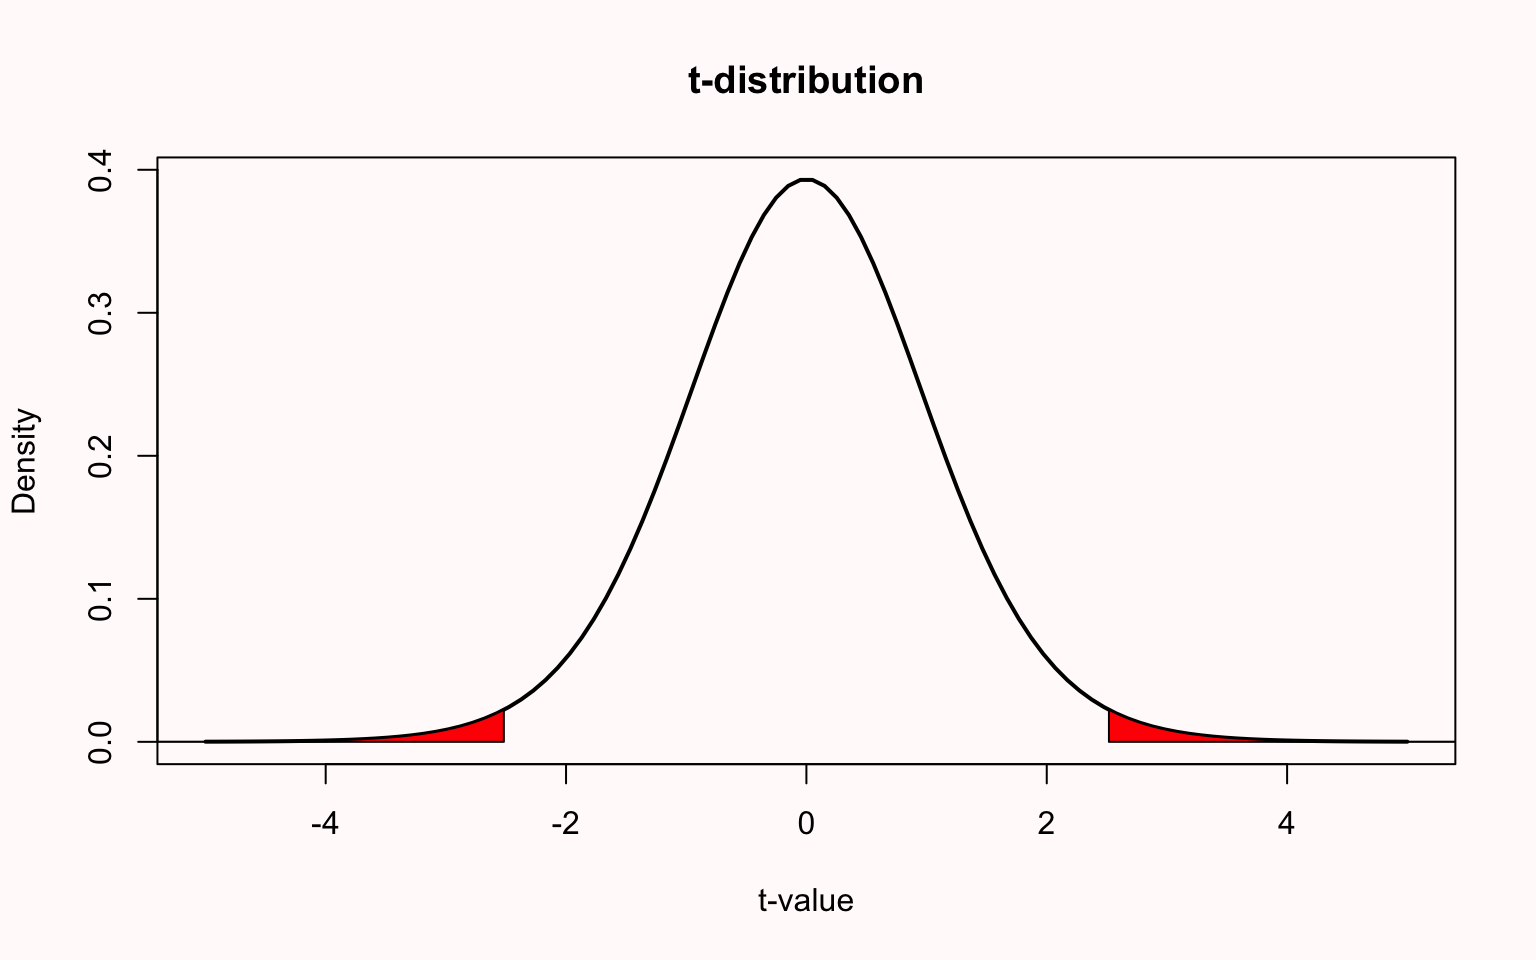
\includegraphics[width=1\linewidth]{01-pvalue_files/figure-latex/tdist-1} 

}

\caption{A \emph{t}-distribution with 18 degrees of freedom.}\label{fig:tdist}
\end{figure}

\hypertarget{whichpexpect}{%
\section{\texorpdfstring{Which \emph{p}-values can you expect?}{Which p-values can you expect?}}\label{whichpexpect}}

In a very educational video about the `\href{https://www.youtube.com/watch?v=5OL1RqHrZQ8}{Dance of the \emph{p}-values}', Geoff Cumming explains that \emph{p}-values vary from experiment to experiment. However, this is not a reason to `not trust p' as he mentions in the video. Instead, it is important to clearly understand \textbf{\emph{p}-value distributions} to prevent misconceptions. Because \emph{p}-values are part of frequentist statistics, we need to examine what we can expect \emph{in the long run}. Because we never do the same experiment hundreds of times, and we do only a very limited number of studies in our lifetime, the best way to learn about what we should expect in the long run is through computer simulations.

Take a moment to try to answer the following two questions. Which \emph{p}-values can you expect to observe if there is a true effect, and you repeat the same study one-hundred thousand times? And which \emph{p}-values can you expect if there is no true effect, and you repeat the same study one-hundred thousand times? If you don't know the answer, don't worry - you will learn it now. But if you don't know the answer, it is worth reflecting on why you don't know the answer about such an essential aspect of \emph{p}-values. If you are like me, you were simply never taught this. But as we will see, it is essential to a solid understanding of how to interpret \emph{p}-values.

Which \emph{p}-values you can expect is completely determined by the statistical power of the study, or the probability that you will observe a significant effect, if there is a true effect. The statistical power ranges from 0 to 1. We can illustrate this by simulating independent \emph{t}-tests. The idea is that we simulate IQ scores for a group of people. We know the standard deviation of IQ scores is 15. For now, we will set the mean IQ score in one simulated group to 100, and in the oher simulated group to 105. We are testing if the people in in one group have an IQ that differs from the other group (and we know the correct answer is `yes', because we made it so in the simulation).

\begin{Shaded}
\begin{Highlighting}[]
\NormalTok{p }\OtherTok{\textless{}{-}} \FunctionTok{numeric}\NormalTok{(}\DecValTok{100000}\NormalTok{) }\CommentTok{\# store all simulated *p*{-}values}

\ControlFlowTok{for}\NormalTok{ (i }\ControlFlowTok{in} \DecValTok{1}\SpecialCharTok{:}\DecValTok{100000}\NormalTok{) \{ }\CommentTok{\# for each simulated experiment}
\NormalTok{  x }\OtherTok{\textless{}{-}} \FunctionTok{rnorm}\NormalTok{(}\AttributeTok{n =} \DecValTok{71}\NormalTok{, }\AttributeTok{mean =} \DecValTok{100}\NormalTok{, }\AttributeTok{sd =} \DecValTok{15}\NormalTok{) }\CommentTok{\# Simulate data}
\NormalTok{  y }\OtherTok{\textless{}{-}} \FunctionTok{rnorm}\NormalTok{(}\AttributeTok{n =} \DecValTok{71}\NormalTok{, }\AttributeTok{mean =} \DecValTok{105}\NormalTok{, }\AttributeTok{sd =} \DecValTok{15}\NormalTok{) }\CommentTok{\# Simulate data}
\NormalTok{  p[i] }\OtherTok{\textless{}{-}} \FunctionTok{t.test}\NormalTok{(x, y)}\SpecialCharTok{$}\NormalTok{p.value }\CommentTok{\# store the *p*{-}value}
\NormalTok{\}}

\NormalTok{(}\FunctionTok{sum}\NormalTok{(p }\SpecialCharTok{\textless{}} \FloatTok{0.05}\NormalTok{) }\SpecialCharTok{/} \DecValTok{100000}\NormalTok{) }\CommentTok{\# compute power}

\FunctionTok{hist}\NormalTok{(p, }\AttributeTok{breaks =} \DecValTok{20}\NormalTok{) }\CommentTok{\# plot a histogram}
\end{Highlighting}
\end{Shaded}

In the simulation, we generate n = 71 normally distributed IQ scores with means of M (100 and 105 by default) and a standard deviation of 15. We then perform an independent \emph{t}-test, store the \emph{p}-value, and generate a plot of the \emph{p}-value distribution.



\begin{figure}

{\centering 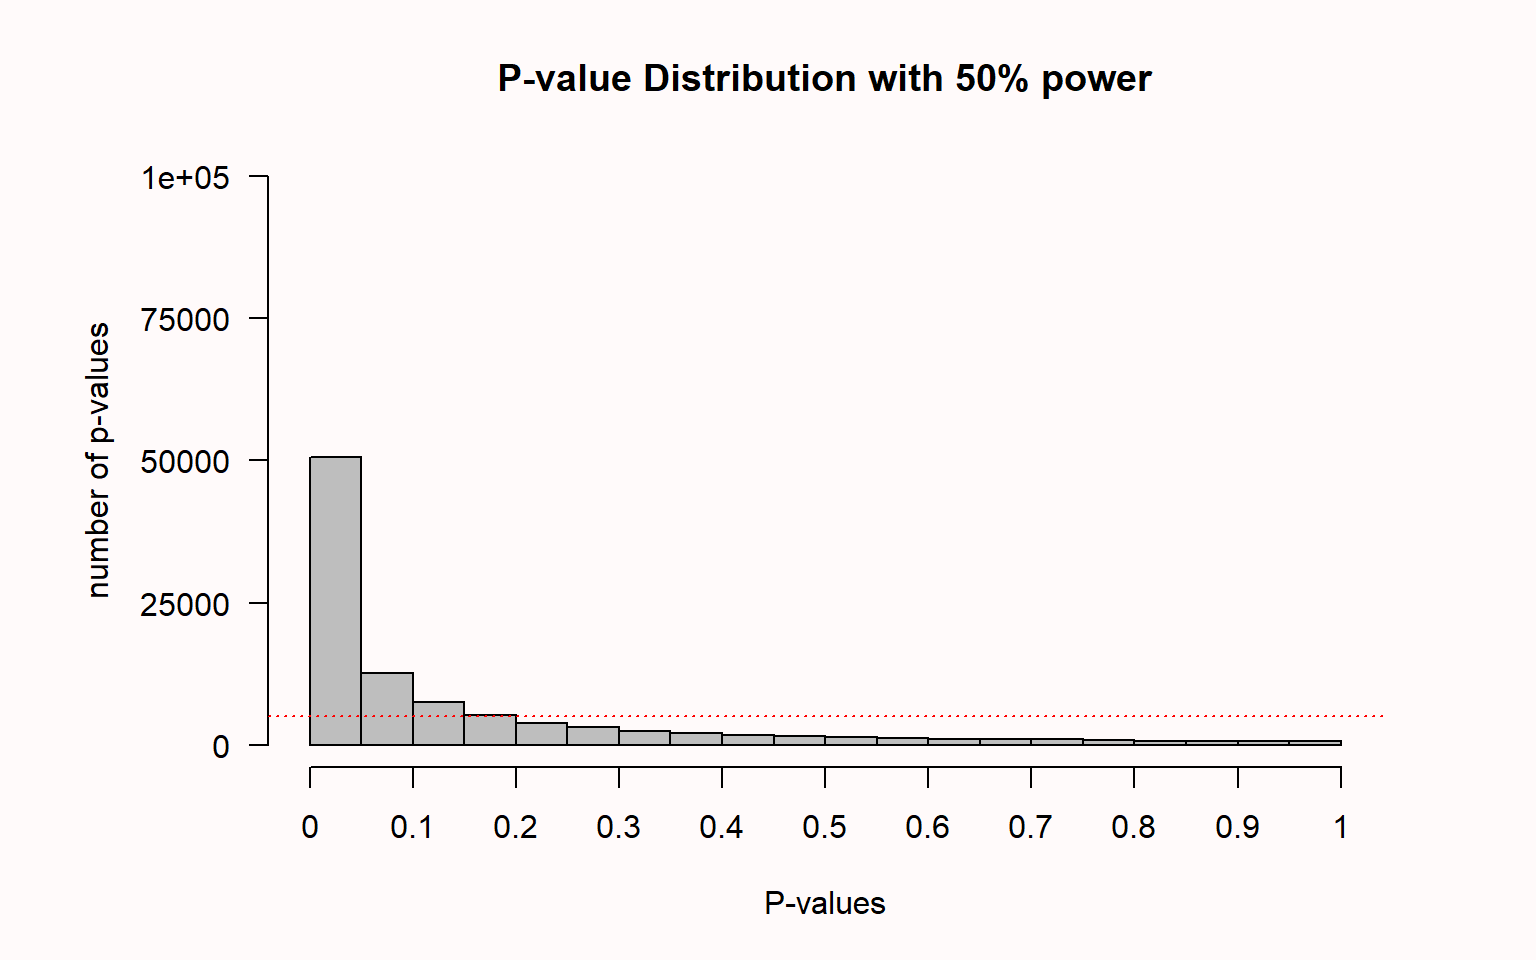
\includegraphics[width=1\linewidth]{01-pvalue_files/figure-latex/pdistr1-1} 

}

\caption{Distribution of \emph{p}-values when power = 50\%.}\label{fig:pdistr1}
\end{figure}

On the x-axis we see \emph{p}-values from 0 to 1 in 20 bars, and on the y-axis we see how frequently these \emph{p}-values were observed. There is a horizontal red dotted line that indicates an alpha of 5\% (located at a frequency of 100.000*0.05 = 5000) -- but you can ignore this line for now. In the title of the graph, the statistical power that is achieved in the simulated studies is given (assuming an alpha of 0.05): The studies have 50\% power.

The simulation result illustrates the \textbf{probability density function} of \emph{p}-values. A probability density function provides the probability that a random variable has a specific value (such as Figure \ref{fig:tdist} of the \emph{t}-distribution). Because the \emph{p}-value is a random variable, we can use its probability density function to plot the \emph{p}-value distribution \citep{hung_behavior_1997, ulrich_properties_2018}, as in Figure \ref{fig:pdft}. You can vary the sample size, effect size, and alpha level in \href{http://shiny.ieis.tue.nl/d_p_power/}{this online Shiny app}. Increasing the sample size or the effect size will increase the steepness of the \emph{p}-value distribution, which means that the probability to observe small \emph{p}-values increases. The \emph{p}-value distribution is a function of the statistical power of the test.



\begin{figure}

{\centering 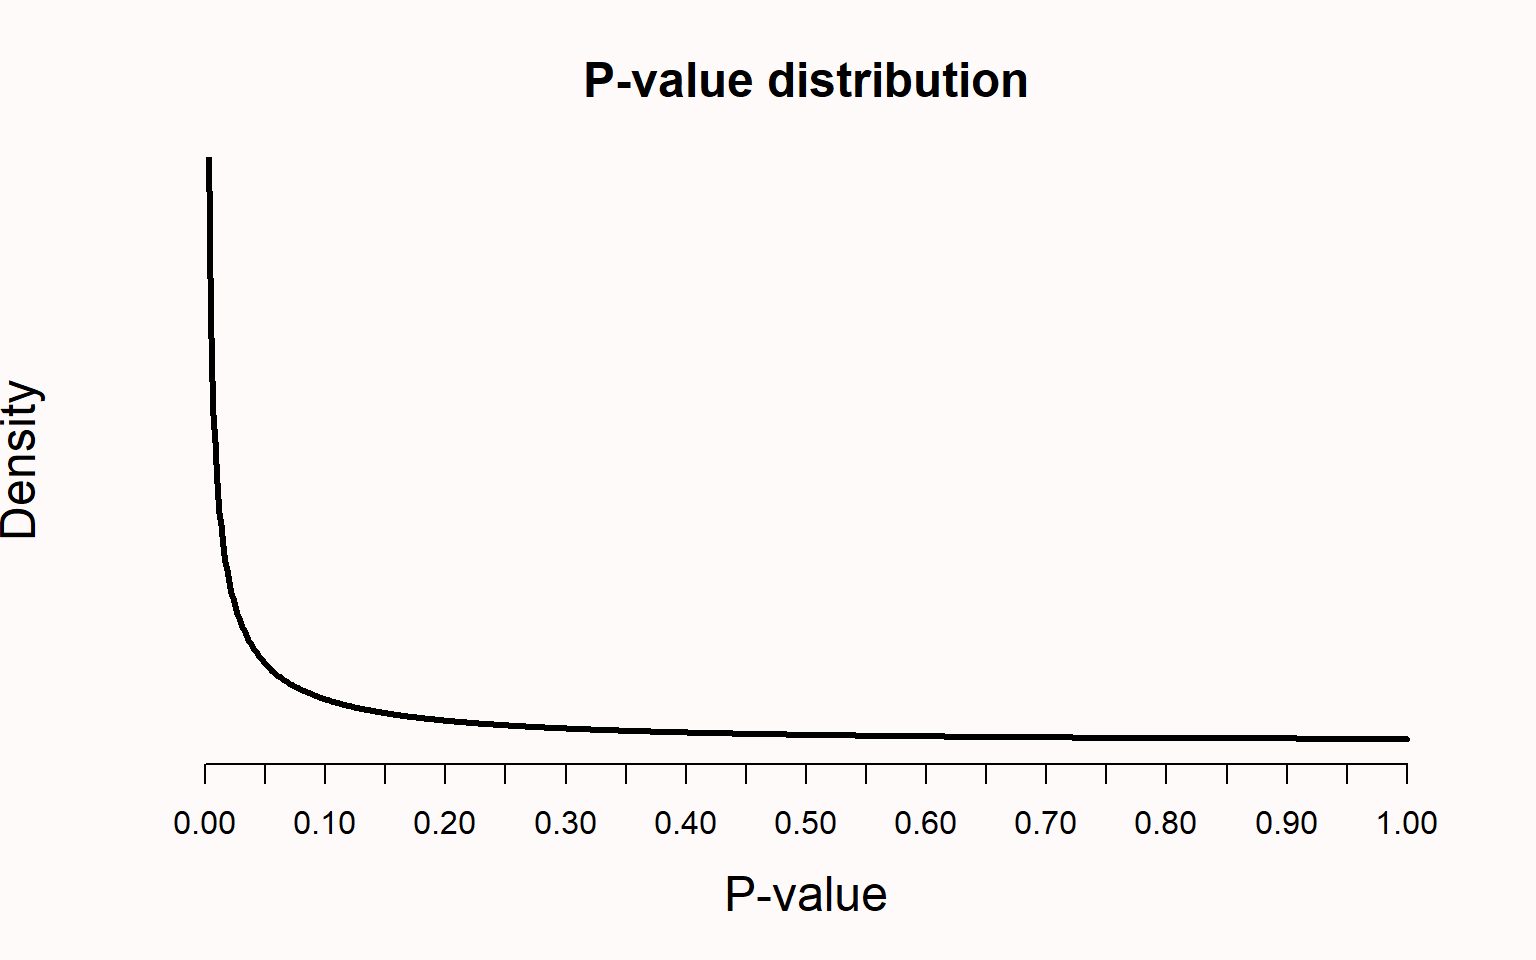
\includegraphics[width=1\linewidth]{01-pvalue_files/figure-latex/pdft-1} 

}

\caption{Probability density function for \emph{p}-values from a two-sided \emph{t}-test.}\label{fig:pdft}
\end{figure}

When there is no true effect, \emph{p}-values are \textbf{uniformly distributed}. This means that every \emph{p}-value is equally likely to be observed when the null hypothesis is true. In other words, when there is no true effect, a \emph{p}-value of 0.08 is just as likely as a \emph{p}-value of 0.98. I remember thinking this was very counterintuitive when I first learned it (well after completing a PhD), but it makes sense when we think of the goal to guarantee that when \(H_0\) is true, alpha \% of the \emph{p}-values fall below the alpha level. If we set alpha to 0.01, 1\% of the observed \emph{p}-values should fall below 0.01, and if we set alpha to 0.12, 12\% of the observed \emph{p}-values should fall below 0.12. This can only happen if \emph{p}-values are uniformly distributed when the null hypothesis is true.



\begin{figure}

{\centering 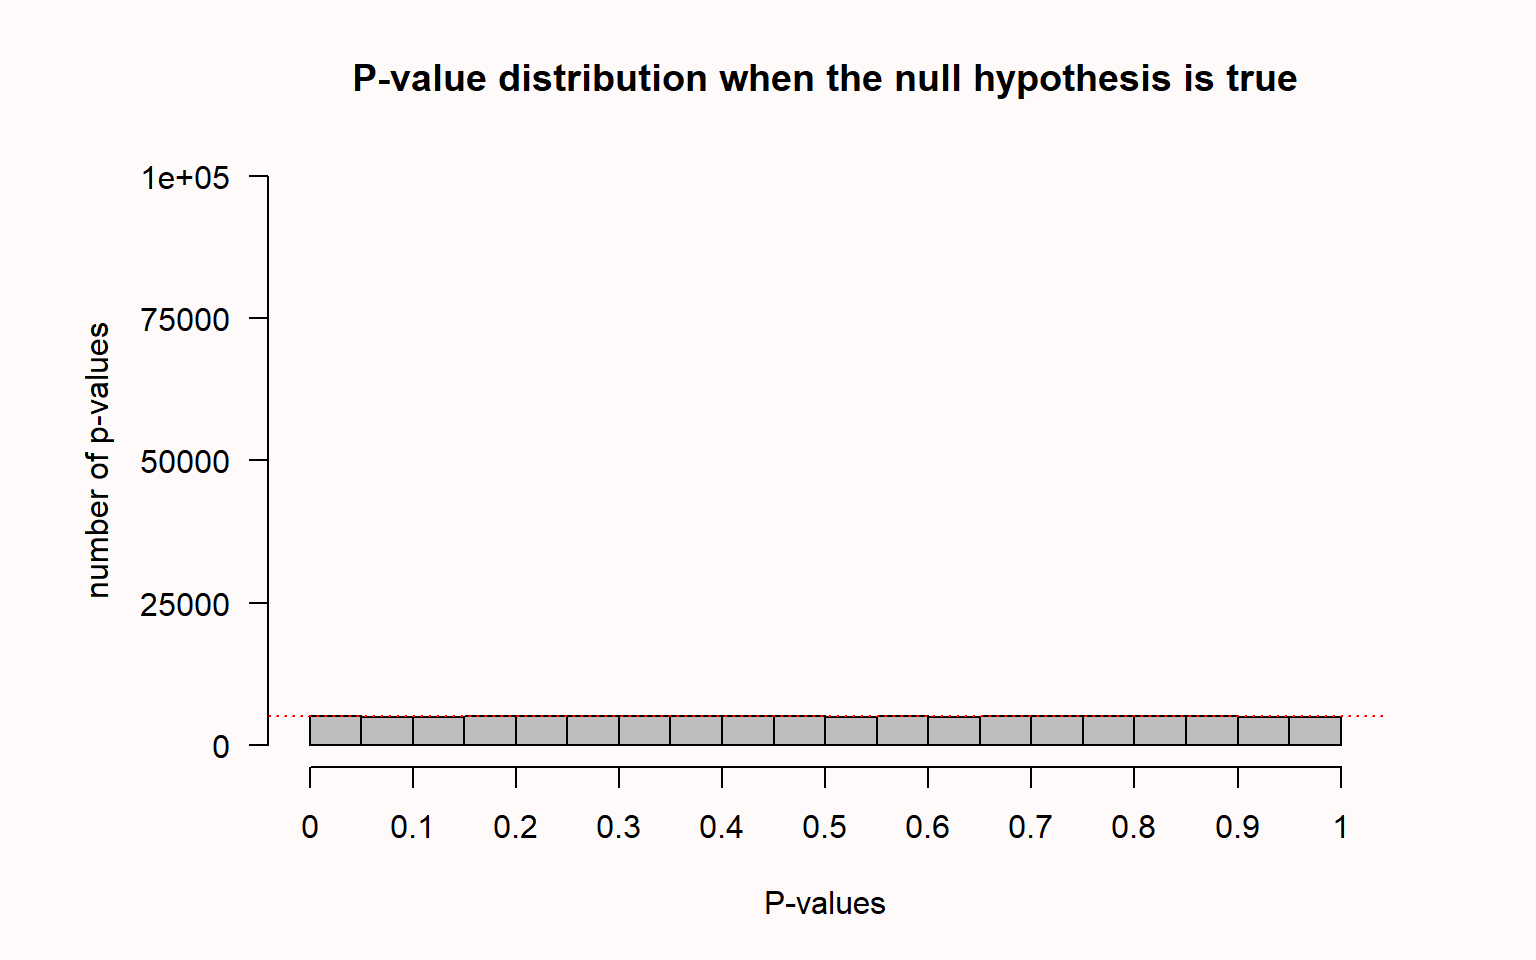
\includegraphics[width=1\linewidth]{01-pvalue_files/figure-latex/pdistr2-1} 

}

\caption{Distribution of \emph{p}-values when the null hypothesis is true.}\label{fig:pdistr2}
\end{figure}

\hypertarget{lindley}{%
\section{Lindley's paradox}\label{lindley}}

As the statistical power increases, some \emph{p}-values below 0.05 (e.g., \emph{p} = 0.04) can be more likely when there is \emph{no} effect than when there \emph{is} an effect. This is known as Lindley's paradox \citep{lindley_statistical_1957}, or sometimes the Jeffreys-Lindley paradox \citep{spanos_who_2013}. Because the distribution of \emph{p}-values is a function of the statistical power \citep{cumming_replication_2008}, the higher the power, the more right-skewed the distribution becomes (i.e., the more likely it becomes that small \emph{p}-values are observed). When there is no true effect, \emph{p}-values are uniformly distributed, and 1\% of observed \emph{p}-values fall between 0.04 and 0.05. When the statistical power is extremely high, not only will most \emph{p}-values fall below 0.05, most \emph{p}-values will fall below 0.01. In Figure \ref{fig:paradox} we see that with high power very small \emph{p}-values (e.g., 0.001) are more likely to be observed when there \emph{is} an effect than when there is \emph{no} effect (e.g., the dotted black curve representing 99\% power falls above the grey horizontal line representing the uniform distribution when the null is true for a \emph{p}-value of 0.01).

Yet perhaps surprisingly, observing a \emph{p}-value of 0.04 is more likely when the null hypothesis (\(H_0\)) is true than when the alternative hypothesis (\(H_1\)) is true and we have very high power, as illustrated by the fact that in Figure \ref{fig:paradox} the density of the \emph{p}-value distribution is higher when the null is true, than when a test has 99\% power, at 0.04. Lindley's paradox shows that a \emph{p}-value of for example 0.04 can be statistically significant, but at the same time is evidence for the null hypothesis. From a Neyman-Pearson approach we have made a claim that has a maximum error rate of 5\%, but from a likelihood or Bayesian approach, we should conclude our data supports the null. Lindley's paradox illustrates when different statistical philosophies would reach different conclusions, and why a \emph{p}-value cannot directly be interpreted as a measure of evidence, without taking the power of the test into account. Although it is not necessary, researchers might desire to prevent situations where a frequentist rejects the null hypothesis based on \emph{p} \textless{} 0.05, when the evidence in the test favors the null hypothesis over the alternative hypothesis. This can be achieved by lowering the alpha level as a function of the sample size \citep{leamer_specification_1978, maier_justify_2022, good_bayesnon-bayes_1992}, as explained in the chapter on \protect\hyperlink{errorcontrol}{error control}.



\begin{figure}

{\centering 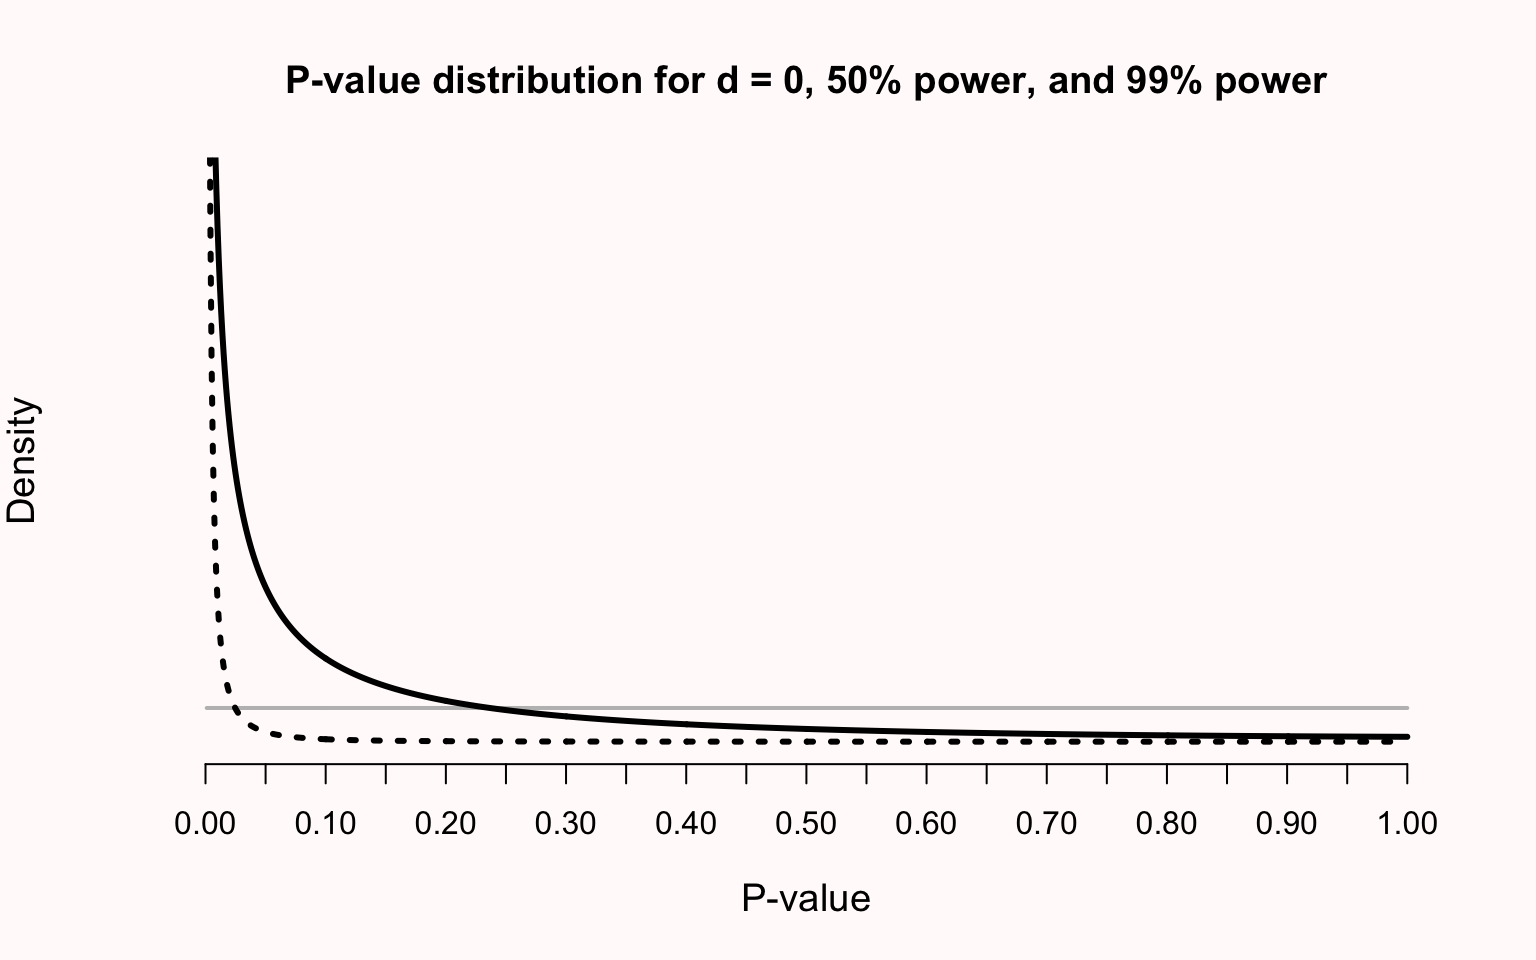
\includegraphics[width=1\linewidth]{01-pvalue_files/figure-latex/paradox-1} 

}

\caption{\emph{P}-value distribution for 0 (grey horizontal line, 50 percent power (black solid curve), and 99 percent power (black dotted curve, where \emph{p}-values just below 0.05 are more likely when \(H_0\) is true than when \(H_1\) is true).}\label{fig:paradox}
\end{figure}

\hypertarget{correctly-reporting-and-interpreting-p-values}{%
\section{\texorpdfstring{Correctly reporting and interpreting \emph{p}-values}{Correctly reporting and interpreting p-values}}\label{correctly-reporting-and-interpreting-p-values}}

Although from a strict Neyman-Pearson perspective it is sufficient to report that \emph{p} \textless{} \(\alpha\) or that \emph{p} \textgreater{} \(\alpha\), researchers should report exact \emph{p}-values. This facilitates the re-use of results for secondary analyses \citep{appelbaum_journal_2018}, and allows other researchers to compare the \emph{p}-value to an alpha level they would have preferred to use \citep{lehmann_testing_2005}. Because claims are made using a methodological procedure with known maximum error rates, a \emph{p}-value never allows you state anything with certainty. Even if we set the alpha level to 0.000001 any single claim can be an error, Fisher \citeyearpar{fisher_design_1935} reminds us, `for the ``one chance in a million'' will undoubtedly occur, with no less and no more than its appropriate frequency, however surprised we may be that it should occur to \emph{us}''. This uncertainty is sometimes not reflected in academic writing, where researchers can be seen using words as 'prove', `show', or `it is known'. A slightly longer but more accurate statement after a hypothesis test would read:

\begin{quote}
We claim there is a/no meaningful effect, while acknowledging that if scientists make claims using this methodological procedure, they will be misled, in the long run, at most alpha \% or beta \% of the time, which we deem acceptable. We will for the foreseeable future, until new data or information emerges that proves us wrong, assume this claim is correct.
\end{quote}

Remember that in a Neyman-Pearson framework researchers make claims, but do not necessarily \emph{believe} in the truth of these claims. For example, the OPERA collaboration reported in 2011 that they had observed data that seemed to suggest neutrinos traveled faster than the speed of light. This claim was made with a with a 0.2-in-a-million Type 1 error rate, \emph{assuming the error was purely due to random noise}. However, none of the researchers actually believed this claim was true, because it is theoretically impossible for neutrinos to move faster than the speed of light. Indeed, it was later confirmed that equipment failures were the cause of the anomalous data: a fiber optic cable had been attached improperly, and a clock oscillator was ticking too fast. Nevertheless, the claim was made with the explicit invitation to the scientific community to provide new data or information that would prove this claim wrong.

When researchers ``accept'' or ``reject'' a hypothesis in a Neyman-Pearson approach to statistical inferences, they do not communicate any belief or conclusion about the substantive hypothesis. Instead, they utter a Popperian \textbf{basic statement} based on a prespecified decision rule that the observed data reflect a certain state of the world. Basic statements describe an observation that has been made (e.g., ``I have observed a black swan'') or an event that has occurred (e.g., ``students performed better at the exam when being trained in spaced practice, than when not'').

The claim is about the data we have observed, but not about the theory we used to make predictions. The claim is about observed data, as it is a statistical inference, and not about the theory, which requires a theoretical inference. Data never `proves' a theory is true or false. A basic statement can \textbf{corroborate} a prediction derived from a theory, or not. If many predictions deduced from a theory are corroborated, we can become increasingly convinced the theory is close to the truth. This `truth-likeness' of theories is called \textbf{verisimilitude} \citep{niiniluoto_verisimilitude_1998, popper_logic_2002}. A shorter statement when a hypothesis test is presented would therefore read `p = .xx, which corroborates our prediction, at an alpha level of y\%', or `p = .xx, which does not corroborate our prediction, at a statistical power of y\% for our effect size of interest'. Often, the alpha level or the statistical power is only mentioned in the experimental design section of an article, but repeating them in the results section might remind readers of the error rates associated with your claims.

Even when we have made correct claims, the underlying theory can be false. Popper \citeyearpar{popper_logic_2002} reminds us that ``The empirical basis of objective science has thus nothing `absolute' basis about it''. He argues science is not built on a solid bedrock, but on piles driven in a swamp and notes that ``We simply stop when we are satisfied that the piles are firm enough to carry the structure, at least for the time being.'' As Hacking \citeyearpar{hacking_logic_1965} writes: ``Rejection is not refutation. Plenty of rejections must be only tentative.'' So when we reject the null model, we do so tentatively, aware of the fact we might have done so in error, without necessarily believing the null model is false, and without believing the theory we have used to make predictions is true. For Neyman \citeyearpar{neyman_inductive_1957} inferential behavior is an: ``act of will to behave in the future (perhaps until new experiments are performed) in a particular manner, conforming with the outcome of the experiment''. All knowledge in science is provisional.

Some statisticians recommend interpreting \emph{p}-values as measures of \emph{evidence}. For example, Bland \citeyearpar{bland_introduction_2015} teaches that \emph{p}-values can be interpreted as a `rough and ready' guide for the strength of evidence, and that \emph{p} \textgreater{} 0.1 indicates `little or no evidence', 0.01 \textless{} \emph{p} \textless{} 0.05 indicates `evidence', \emph{p} \textless{} 0.001 is `very strong evidence'. This is incorrect \citep{lakens_why_2022}, as is clear from the previous discussions of Lindley's paradox and uniform \emph{p}-value distributions. If you want to quantify \emph{evidence}, see the chapters on \protect\hyperlink{likelihoods}{likelihoods} or \protect\hyperlink{bayes}{Bayesian statistics}.

\hypertarget{misconceptions}{%
\section{\texorpdfstring{Preventing common misconceptions about \emph{p}-values}{Preventing common misconceptions about p-values}}\label{misconceptions}}

A \emph{p}-value is the probability of the observed data, or more extreme data, under the assumption that the null hypothesis is true. To understand what this means, it might be especially useful to know what this doesn't mean. First, we need to know what `the assumption that the null hypothesis is true' looks like, and which data we should expect if the null hypothesis is true. Although the null hypothesis can be any value, in this assignment we will assume the null hypothesis is specified as a mean difference of 0. For example, we might be interested in calculating the difference between a control condition and an experimental condition on a dependent variable.

It is useful to distinguish the null hypothesis (the prediction that the mean difference in the population is exactly 0) and the null model (a model of the data we should expect when we collect data when the null hypothesis is true). The null hypothesis is a point at 0, but the null model is a distribution. It is visualized in textbooks or power analysis software using pictures as you can see below, with \emph{t}-values on the horizontal axis, and a critical \emph{t}-value somewhere between 1.96 -- 2.00 (depending on the sample size). This is done because the statistical test when comparing two groups is based on the \emph{t}-distribution, and the \emph{p}-value is statistically significant when the \emph{t}-value is larger than a critical \emph{t}-value.

I personally find things become a lot clearer if you plot the null model as mean differences instead of \emph{t}-values. So below, you can see a null model for the mean differences we can expect when comparing two groups of 50 observations where the true difference between the two groups is 0, and the standard deviation in each group is 1. Because the standard deviation is 1, you can also interpret the mean differences as a Cohen's \emph{d} effect size. So this is also the distribution you can expect for a Cohen's \emph{d} of 0, when collecting 50 observations per group in an independent \emph{t}-test.



\begin{figure}

{\centering 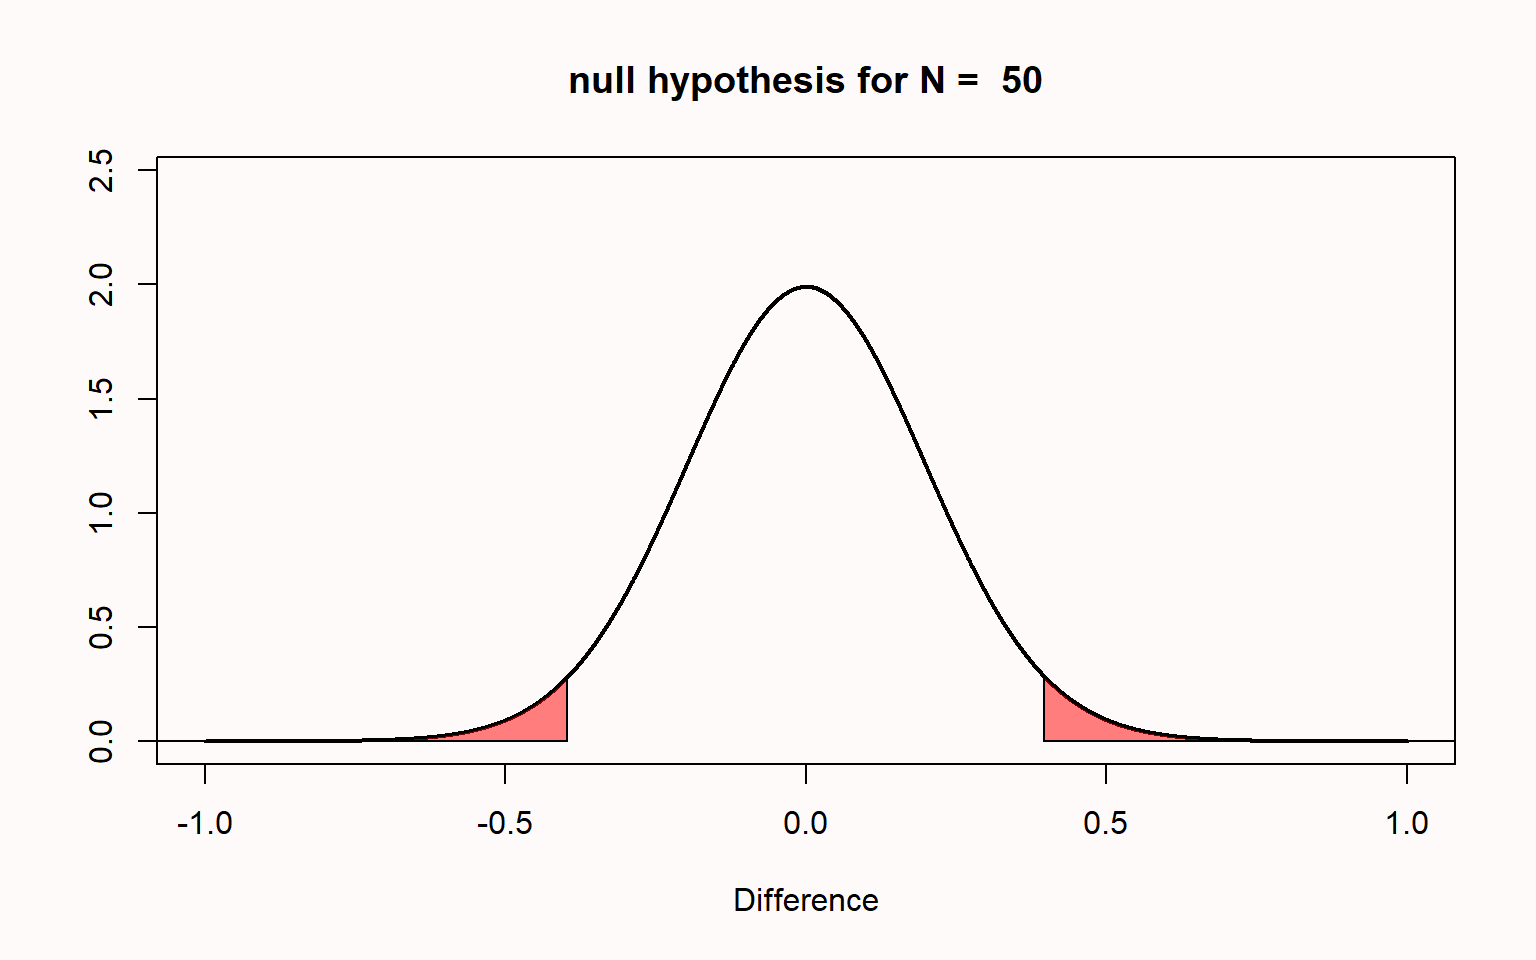
\includegraphics[width=1\linewidth]{01-pvalue_files/figure-latex/fig131-1} 

}

\caption{Distribution of observed Cohen's \emph{d} effect sizes when collecting 50 observations per group in an independent \emph{t}-test.}\label{fig:fig131}
\end{figure}

The first thing to notice is that we expect that the mean of the null model is 0. Looking at the x-axis, we see the plotted distribution is centered on 0. But even if the mean difference in the population is 0 that does not imply every sample we draw from the population will give a mean difference of exactly zero. There is variation around the population value, as a function of the standard deviation and the sample size.

The y-axis of the graph represents the density, which provides an indication of the relative likelihood of measuring a particular value of a continuous distribution. We can see that the most likely mean difference is the true population value of zero, and that larger differences from zero become increasingly less likely. The graph has two areas that are colored red. These areas represent 2.5\% of the most extreme values in the left tail of the distribution, and 2.5\% of the most extreme values in the right tail of the distribution. Together, they make up 5\% of the most extreme mean differences we would expect to observe, given our number of observations, when the true mean difference is exactly 0. When a mean difference in the red area is observed, the corresponding statistical test will be statistically significant at a 5\% alpha level. In other words, not more than 5\% of the observed mean differences will be far enough away from 0 to be considered surprising. Because the null hypothesis is true, observing a `surprising' mean difference in the red areas is a Type 1 error.

Let's assume that the null model in the Figure above is true, and that we observe a mean difference of 0.5 between the two groups. This observed difference falls in the red area in the right tail of the distribution. This means that the observed mean difference is relatively surprising, under the assumption that the true mean difference is 0. If the true mean difference is 0, the probability density functions shows that we should not expect a mean difference of 0.5 very often. If we calculate a \emph{p}-value for this observation, it would be lower than 5\%. The probability of observing a mean difference that is at least as far away from 0 as 0.5 (either to the left from the mean, or to the right, when we do a two-tailed test) is less than 5\%.

One reason why I prefer to plot the null model in raw scores instead of \emph{t}-values is that you can see how the null model changes when the sample size increases. When we collect 5000 instead of 50 observations, we see the null model is still centered on 0 -- but in our null model we now expect most values will fall very close around 0.



\begin{figure}

{\centering 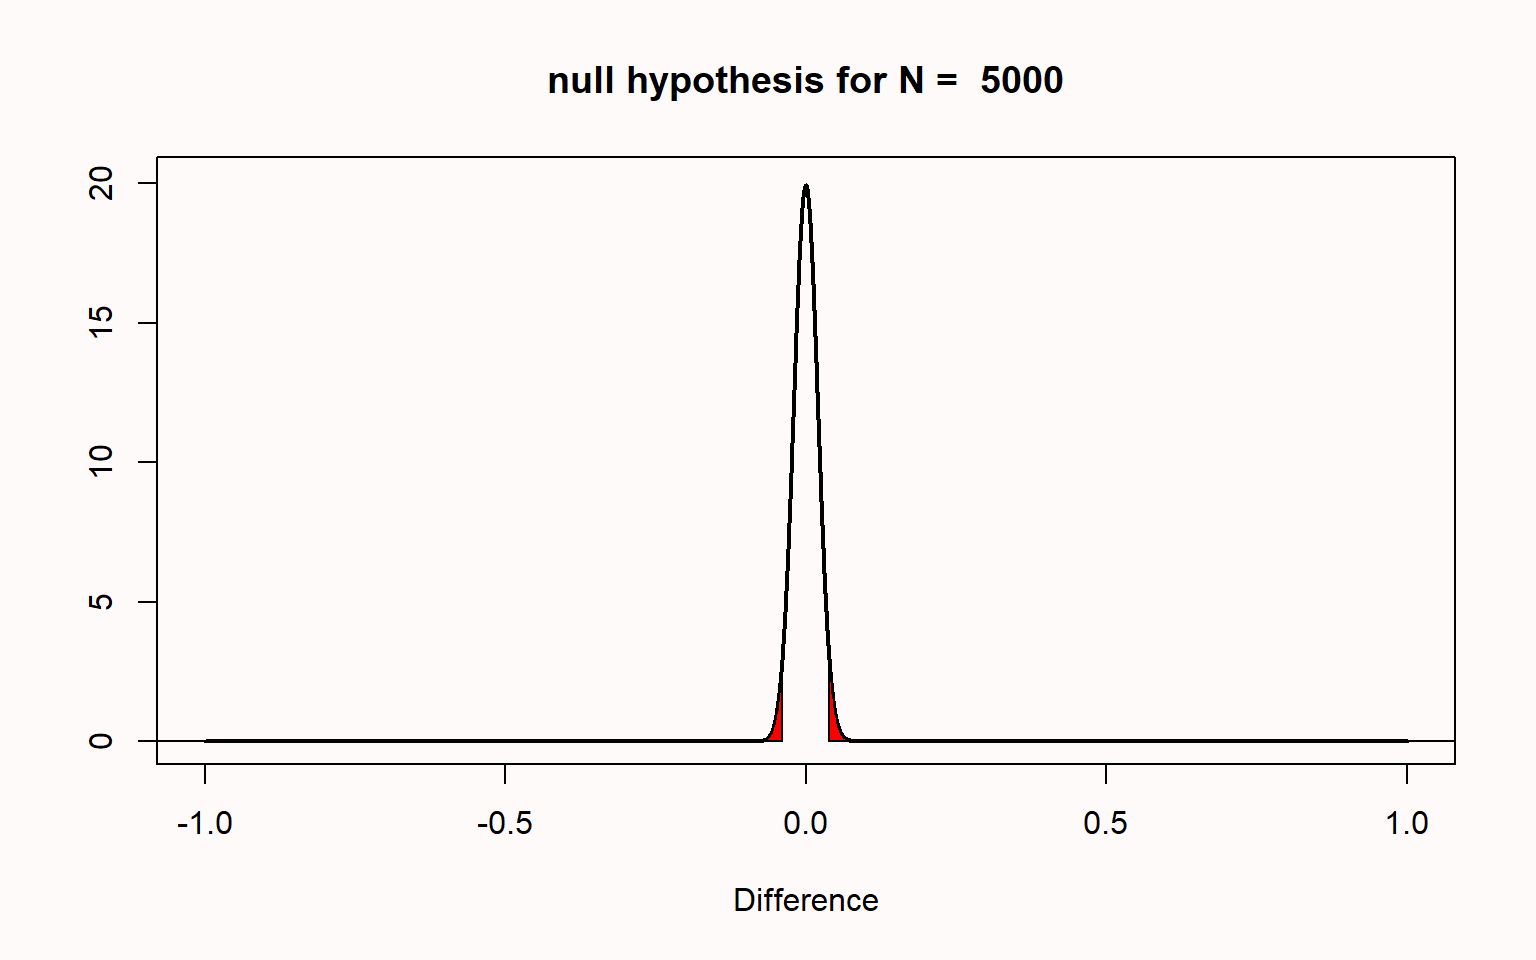
\includegraphics[width=1\linewidth]{01-pvalue_files/figure-latex/fig132-1} 

}

\caption{Distribution of observed Cohen's \emph{d} effect sizes when collecting 5000 observations per group in an independent \emph{t}-test when \emph{d} = 0.}\label{fig:fig132}
\end{figure}

The distribution is much narrower because the distribution of mean differences is based on the standard error of the difference between means. This value is calculated based on the standard deviation and the sample size, as follows:

\[\sqrt{\frac{\sigma_{1}^{2}}{n_{1}}+\frac{\sigma_{2}^{2}}{n_{2}}}\]

This formula shows that the standard deviations of each group (σ) are squared and divided by the sample size of that group, added together, after which the square root is taken. The larger the sample size the bigger the number we divide by, and thus the smaller standard error of the difference between means. In our n = 50 example this is:

\[\sqrt{\frac{1^{2}}{50}+\frac{1^{2}}{50}}\]

The standard error of the differences between means is thus 0.2 for n = 50 in each group, and for n = 5000 it is 0.02. Assuming a normal distribution, 95\% of the observations fall between 1.96 SE. So for 50 samples per group, the mean differences should fall between -1.96 * 0.2 = -0.392, and +1.96 * 0.2 = 0.392, and we can see the red areas start from approximately -0.392 to 0.392 for n = 50. For 5000 samples per group, the mean differences should fall between -1.96 * 0.02, and +1.96 * 0.02; in other words between -0.0392 to 0.0392 for n = 5000. Due to the larger sample size with n = 5000 observations per group, we should expect to observe mean differences in our sample closer to 0 compared to our null model when we had only 50 observations.

If we collected n = 5000, and we would again observe a mean difference of 0.5, it should be clear that this same difference is even more surprising than it was when we collected 50 observations. We are now almost ready to address common misconceptions about \emph{p}-values, but before we can do this, we need to introduce a model of the data when the null is not true. If we are not sampling data from a model where the true mean difference is 0, what does our alternative model look like? Some software (such as G*power, see Figure \ref{fig:gpowerscreenshot}) will visualize both the null model (red curve) and the alternative model (blue curve) in their output:



\begin{figure}

{\centering 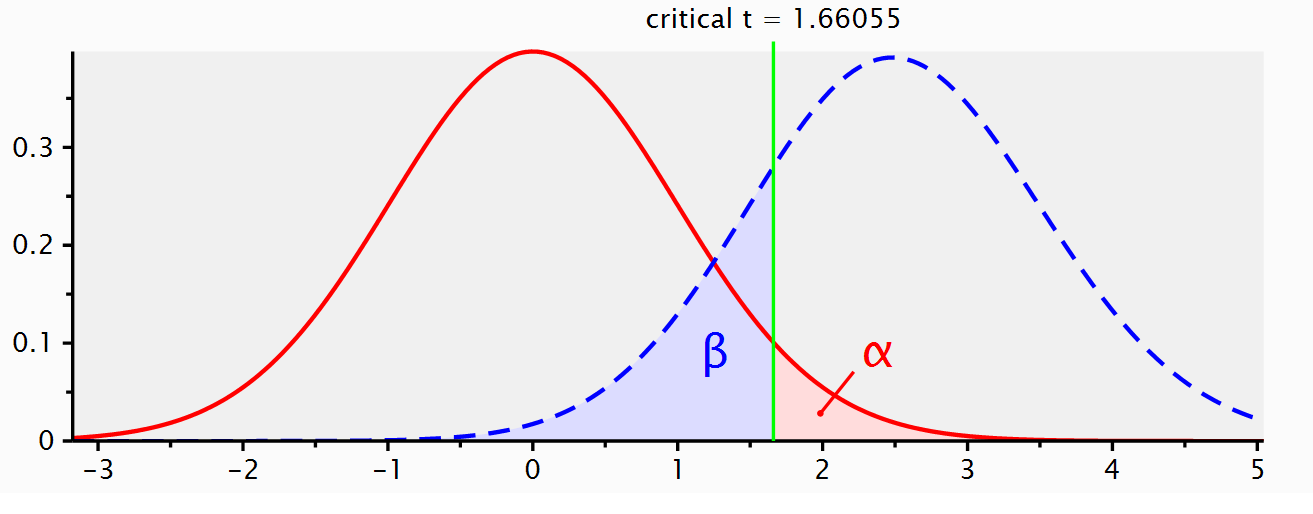
\includegraphics[width=1\linewidth]{images/1.3.3} 

}

\caption{Screenshot from G*Power software visualizing the null model (red distribution) and alternative model (blue distribution) and the critical \emph{t}-value (1.66055) that is the threshold distinguishing significant and non-significant results.}\label{fig:gpowerscreenshot}
\end{figure}

When we do a study, we rarely already know what the true mean difference is (if we already knew, why would we do the study?). But let's assume there is an all-knowing entity. Following Paul Meehl, we will call this all-knowing entity `Omniscient Jones'. Before we collect our sample of 50 observations, Omniscient Jones already knows that the true mean difference in the population is 0.5. Again, we should expect some variation around 0.5 in this alternative model. The figure below shows the expected data pattern when the null hypothesis is true (now indicated by a grey line) and it shows an alternative model, assuming a true mean difference of 0.5 exists in the population (indicated by a black line).



\begin{figure}

{\centering 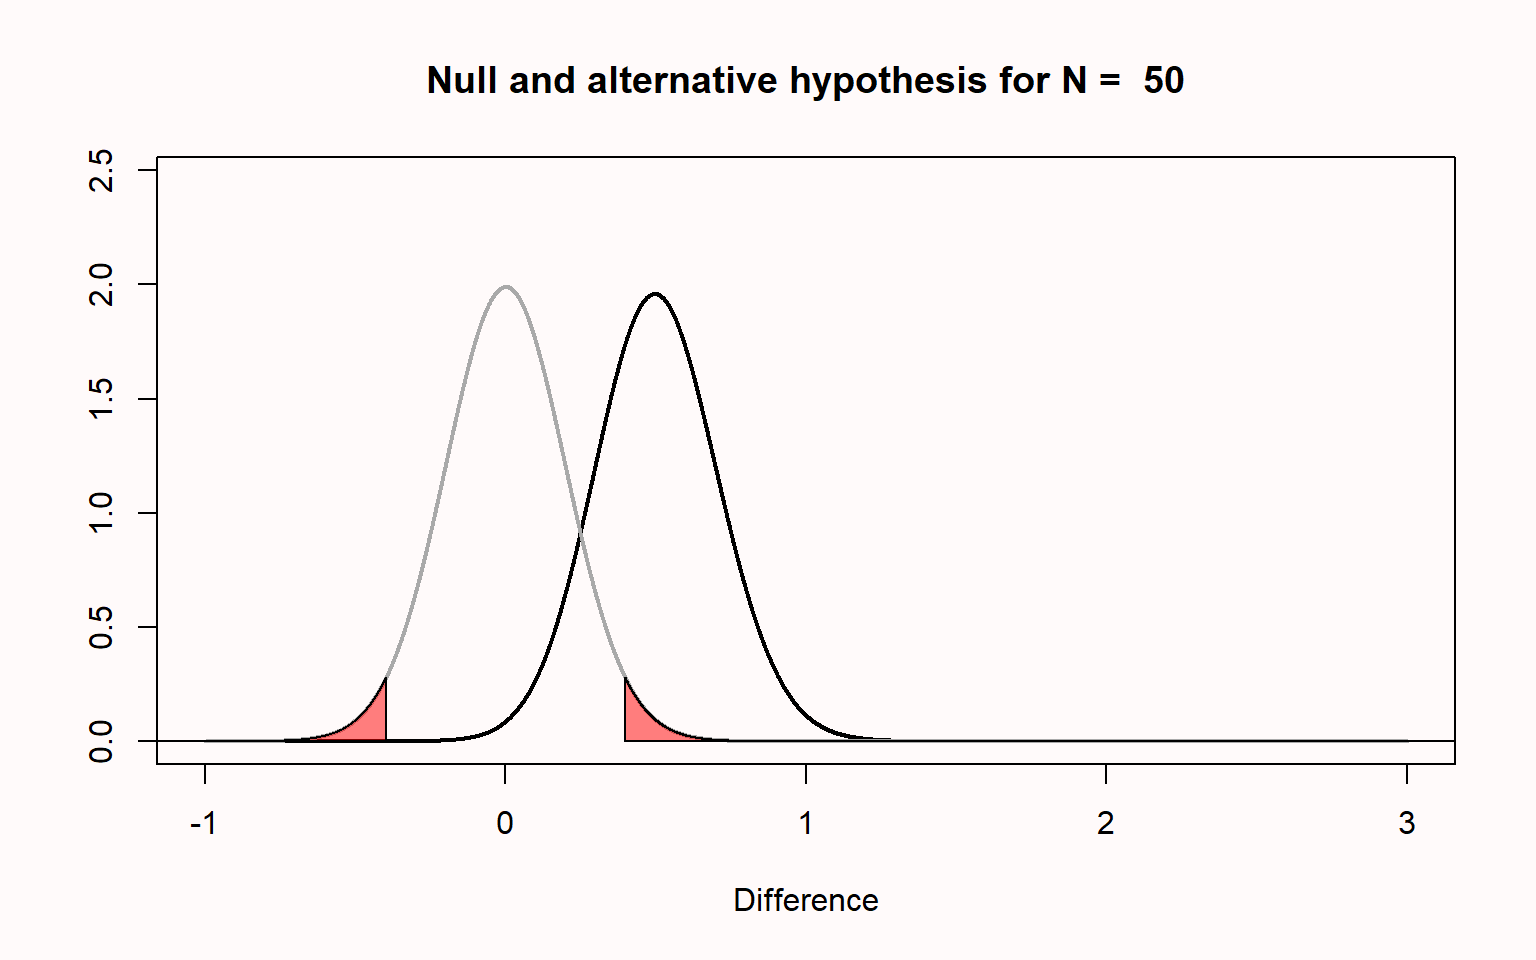
\includegraphics[width=1\linewidth]{01-pvalue_files/figure-latex/fig134-1} 

}

\caption{Distribution of observed Cohen's \emph{d} effect sizes when collecting 50 observations per group in an independent \emph{t}-test when \emph{d} = 0.}\label{fig:fig134}
\end{figure}

But Omniscient Jones could have said the true difference was much larger. Let's assume we do another study, but now before we collect our 50 observations, Omniscient Jones tells us that the true mean difference is 1.5. The null model does not change, but the alternative model now moves over to the right.



You can play around with the alternative and null models in this online app: \url{http://shiny.ieis.tue.nl/d_p_power/}. The app allows you to specify the sample size in each group of an independent \emph{t}-test (from 2 to infinity), the mean difference (from 0 to 2), and the alpha level. In the plot, the red areas visualize Type 1 errors. The blue area visualizes the Type 2 error rate (which we will discuss below). The app also tells you the critical value: There is a vertical line (with n = 50 this line falls at a mean difference of 0.4) and a sentence that says: ``Effects larger than 0.4 will be statistically significant''. Note that the same is true for effects smaller than -0.4, even though there is no second label there, but the app shows the situation for a two-sided independent \emph{t}-test.

You can see that on the left of the vertical line that indicates the critical mean difference there is a blue area that is part of the alternative model. This is the Type 2 error rate (or 1 - the power of the study). If a study has 80\% power, 80\% of the mean differences we will observe should fall on the right of the critical value indicated by the line. If the alternative model is true, but we observe an effect smaller than the critical value, the observed \emph{p}-value will be larger than 0.05, even when there is a true effect. You can check in the app that the larger the sample size, the further to the right the entire alternative distribution falls, and thus the higher the power. You can also see that the larger the sample size, the narrower the distribution, and the less of the distribution will fall below the critical value (as long as the true population mean is larger than the critical value). Finally, the larger the alpha level, the further to the left the critical mean difference moves, and the smaller the area of the alternative distribution that falls below the critical value.

The app also plots 3 graphs that illustrate the power curves as a function of different alpha levels, sample sizes, or true mean differences. Play around in the app by changing the values. Get a feel for how each variable impacts the null and alternative models, the mean difference that will be statistically significant, and the Type 1 and Type 2 error rates.

So far, several aspects of null models should have become clear. First of all, the population value in a traditional null hypothesis is a value of 0, but in any sample you draw, the observed difference falls in a distribution centered on 0, and will thus most often be slightly larger or smaller than 0. Second, the width of this distribution depends on the sample size and the standard deviation. The larger the sample size in the study, the narrower the distribution will be around 0. Finally, when a mean difference is observed that falls in the tails of the null model, this can be considered surprising. The further away from the null value, the more surprising this result is. But when the null model is true, these surprising values will happen with a probability specified by the alpha level (and are called Type 1 errors). Remember that a Type 1 error occurs when a researcher concludes there is a difference in the population, while the true mean difference in the population is zero.

We are now finally ready to address some common misconceptions about \emph{p}-values. Let's go through a list of common misconceptions that have been reported in the scientific literature. Some of these examples might sound like semantics. It is easy to at first glance think that the statement communicates the right idea, even if the written version is not formally correct. However, when a statement is not formally correct, it is wrong. And exactly because people so often misunderstand \emph{p}-values, it is worth it to be formally correct about how they should be interpreted.

\hypertarget{misconception1}{%
\subsection{\texorpdfstring{Misunderstanding 1: A non-significant \emph{p}-value means that the null hypothesis is true.}{Misunderstanding 1: A non-significant p-value means that the null hypothesis is true.}}\label{misconception1}}

A common version of this misconception is reading a sentence such as `because \emph{p} \textgreater{} 0.05 we can conclude that there is no effect'. Another version of such a sentence is `there was no difference, (\emph{p} \textgreater{} 0.05)'.

Before we look at this misconception in some detail, I want to remind you of one fact that is easy to remember, and will enable you to recognize many misconceptions about \emph{p}-values: \emph{p}-values are a statement about the probability of data, not a statement about the probability of a hypothesis or the probability of a theory. Whenever you see \emph{p}-values interpreted as a probability of a theory or a hypothesis, you know something is not right. Examples of statements about a hypothesis are `The null hypothesis is true', or `The alternative hypothesis is true', because both these statements say that the probability that the null or alternative model is true is 100\%. A subtler version is a statement such as `the observed difference is not due to chance'. The observed difference is only `due to chance' (instead of due to the presence of a real difference) when the null hypothesis is true, and as before, this statement implies it is 100\% probable that the null hypothesis is true.

When you conclude that `there is no effect' or that `there is no difference' you are similarly claiming that it is 100\% probable that the null hypothesis is true. But since \emph{p}-values are statements about the probability of data, you should refrain from making statements about the probability of a theory solely based on a \emph{p}-value. That's ok. \emph{p}-values were designed to help you identify surprising results from a noisy data generation process (aka the real world). They were not designed to quantify the probability that a hypothesis is true.

Let's take a concrete example that will illustrate why a non-significant result does not mean that the null hypothesis is true. In the figure below, Omniscient Jones tells us the true mean difference is 0.5. We can see this, because the alternative distribution which visualizes the probability of the mean differences we should expect when the alternative hypothesis is true is centered on 0.5. We have observed a mean difference of 0.35. This value is not extreme enough to be statistically different from 0. We can see this, because the value does not fall within the red area of the null model (and hence, the \emph{p}-value is not smaller than our alpha level).

Nevertheless, we see that observing a mean difference of 0.35 is not only quite likely given that the true mean difference is 0.5, but observing a mean difference of 0.35 is much more likely under the alternative model than under the null model. You can see this by comparing the height of the density curve at a difference of 0.35 for the null model, which is approximately 0.5, and the height of the density curve for the alternative model, which is approximately 1.5. See the chapter on \protect\hyperlink{likettest}{likelihoods} for further details.



\begin{figure}

{\centering 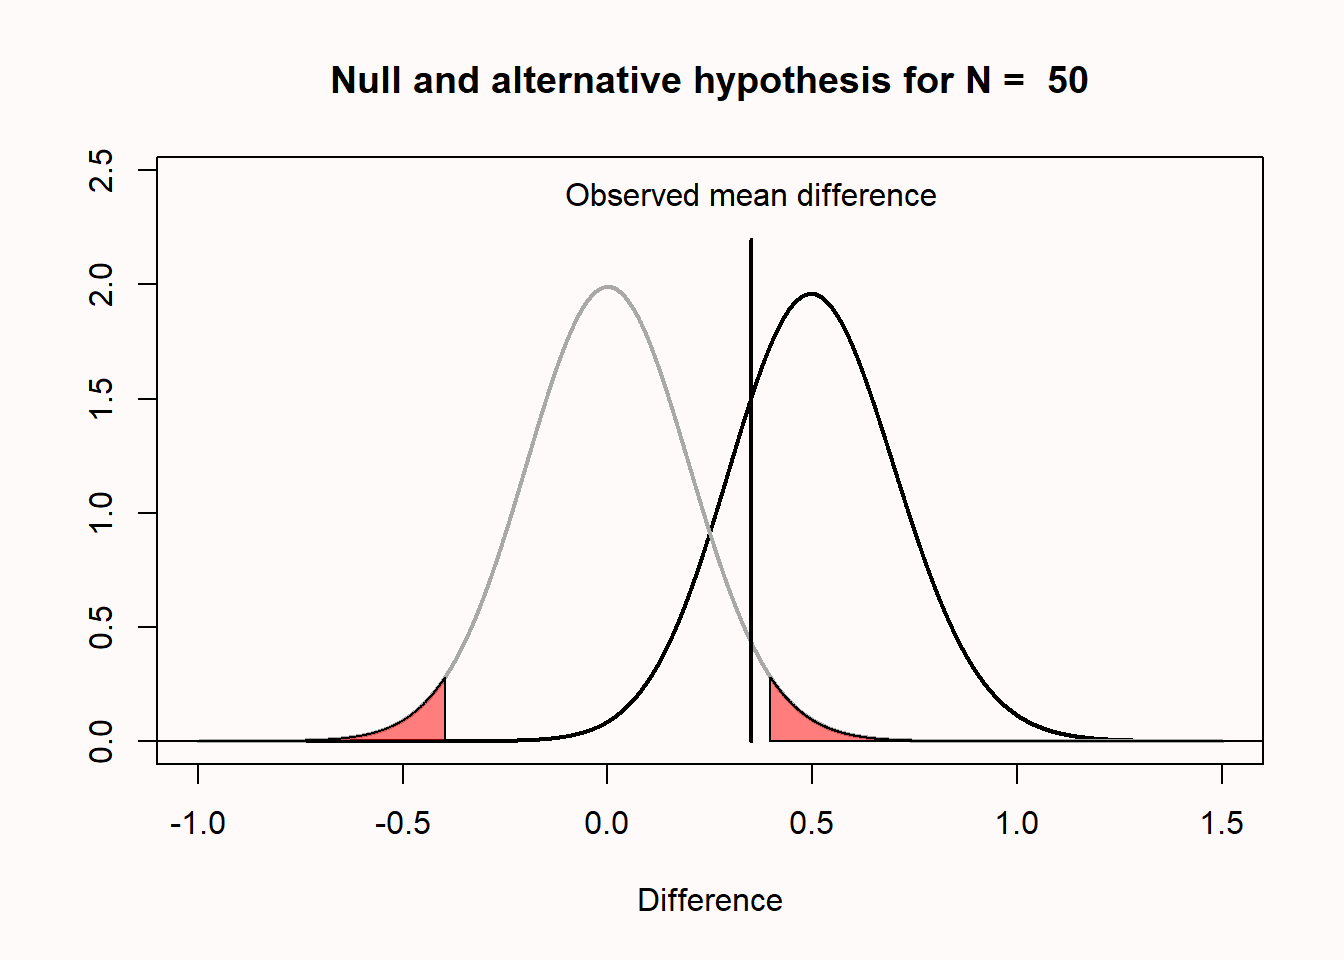
\includegraphics[width=1\linewidth]{01-pvalue_files/figure-latex/fig136-1} 

}

\caption{Distribution of observed Cohen's \emph{d} effect sizes when collecting 50 observations per group in an independent t-test for \emph{d} = 0 and \emph{d} = 0.5 when observing \emph{d} = 0.35.}\label{fig:fig136}
\end{figure}

All the \emph{p}-value tells us is that a mean difference of 0.35 is not extremely surprising, if we assume the null hypothesis is true. There can be many reasons for this. In the real world, where we have no Omniscient Jones to tell us about the true mean difference, it is possible that there is a true effect, as illustrated in the figure above.

So what should we say instead? The solution is subtle, but important. Let's revisit the two examples of incorrect statements we made earlier. First, `because \emph{p} \textgreater{} 0.05 we can conclude that there is no effect' is incorrect, because there might very well be an effect (and remember \emph{p}-values are statements about data, not about the probability that there is an effect or is no effect). Fisher's interpretation of a \emph{p}-value was that we can conclude a rare event has happened, or that the null hypothesis is false (he writes literally: ``Either an exceptionally rare chance has occurred, or the theory of random distribution is not true''). This might sound like it is a statement about the probability of a theory, but it is really just stating the two possible scenarios under which low \emph{p}-values occur (when you have made a Type 1 error, or when the alternative hypothesis is true). Both a true positive as a false positive remain possible, and we do not quantify the probability of either possible reality (e.g., we are not saying it is 95\% probable that the null hypothesis is false). From a Neyman-Pearson perspective, a \emph{p} \textgreater{} .05 means that we cannot act as if the null hypothesis can be rejected, without maintaining our desired error rate of 5\%.

If you are interested in concluding an effect is absent, null hypothesis testing is not the tool to use. A null hypothesis test answers the question `can I reject the null hypothesis with a desired error rate?'. If you cannot do this, and p \textgreater{} 0.05, no conclusion can be drawn based only on the \emph{p}-value (remember the concept of 無 `mu': the answer is neither yes nor no). Luckily, statistical approaches have been developed to ask questions about the absence of an effect such as \protect\hyperlink{equivalencetest}{equivalence testing}, Bayes factors, and Bayesian estimation (see \citet{harms_making_2018}, for an overview).

The second incorrect statement was `there was no difference'. This statement is somewhat easier to correct. You can instead write `there was no statistically significant difference'. Granted, this is a bit tautological, because you are basically saying that the \emph{p}-value was larger than the alpha level in two different ways, but at least this statement is formally correct. The difference between `there was no difference' and `there was no statistically significant difference' might sound like semantics, but in the first case you are formally saying `the difference was 0' while in the second you are saying `there was no difference large enough to yield a \emph{p} \textless{} .05'. Although I have never seen anyone do this, a more informative message might be `because given our sample size of 50 per group, and our alpha level of 0.05, only observed differences more extreme than 0.4 could be statistically significant, and our observed mean difference was 0.35 thus we could not reject the null hypothesis'. If this feels like a very unsatisfactory conclusion, remember that a null hypothesis test was not designed to draw interesting conclusions about the absence of effects -- you will need to learn about equivalence tests to get a more satisfactory answers about null effects.

\hypertarget{misunderstanding-2-a-significant-p-value-means-that-the-null-hypothesis-is-false.}{%
\subsection{\texorpdfstring{Misunderstanding 2: A significant \emph{p}-value means that the null hypothesis is false.}{Misunderstanding 2: A significant p-value means that the null hypothesis is false.}}\label{misunderstanding-2-a-significant-p-value-means-that-the-null-hypothesis-is-false.}}

This is the opposite misconception from the one we discussed previously. Examples of incorrect statements based on this misconception are `\emph{p} \textless{} .05, therefore there is an effect', or `there is a difference between the two groups, \emph{p} \textless{} .05'. As before, both these statements imply it is 100\% probable that the null model is false, and an alternative model is true.

As a simple example of why such extreme statements are incorrect, imagine we generate a series of numbers in R using the following command:

\begin{Shaded}
\begin{Highlighting}[]
\FunctionTok{rnorm}\NormalTok{(}\AttributeTok{n =} \DecValTok{50}\NormalTok{, }\AttributeTok{mean =} \DecValTok{0}\NormalTok{, }\AttributeTok{sd =} \DecValTok{1}\NormalTok{)}
\end{Highlighting}
\end{Shaded}

\begin{verbatim}
##  [1] -0.46109600 -2.25402496  0.20512299  1.09360440 -0.15293644 -1.24966288
##  [7]  1.01390480  0.76911906  1.14802389  0.51456713 -1.09018659 -1.55496645
## [13] -1.03898482  0.08234471 -0.85364786  0.96708697 -0.37131174  0.66731101
## [19] -0.86293939 -0.04236545 -0.17720631 -0.52018260  0.09420899  0.35805351
## [25] -0.59089638 -1.29270044 -0.21817200 -1.64399900 -0.44819759 -0.41481146
## [31] -1.70034641 -0.87135056 -0.03435521 -1.00361633  0.85359694  0.08253064
## [37]  1.26274633  0.51062086 -2.21589299  0.51892733  1.90720700  1.18199783
## [43] -0.22897471 -1.08535386 -0.06155283 -0.83213659  0.81791260 -1.36685454
## [49] -1.39100887  1.14728856
\end{verbatim}

This command generates 50 random observations from a distribution with a mean of 0 and a standard deviation of 1 (in the long run -- the mean and standard deviation will vary in each sample that is generated). Imagine we run this command once, and we observe a mean of 0.5. The figure below visualizes this scenario. We can perform a one-sample \emph{t}-test against 0, and this test tells us, with a \emph{p} \textless{} .05, that the data we have observed is surprisingly different from 0, assuming the random number generator in R functions as it should and generates data with a true mean of 0.



\begin{figure}

{\centering 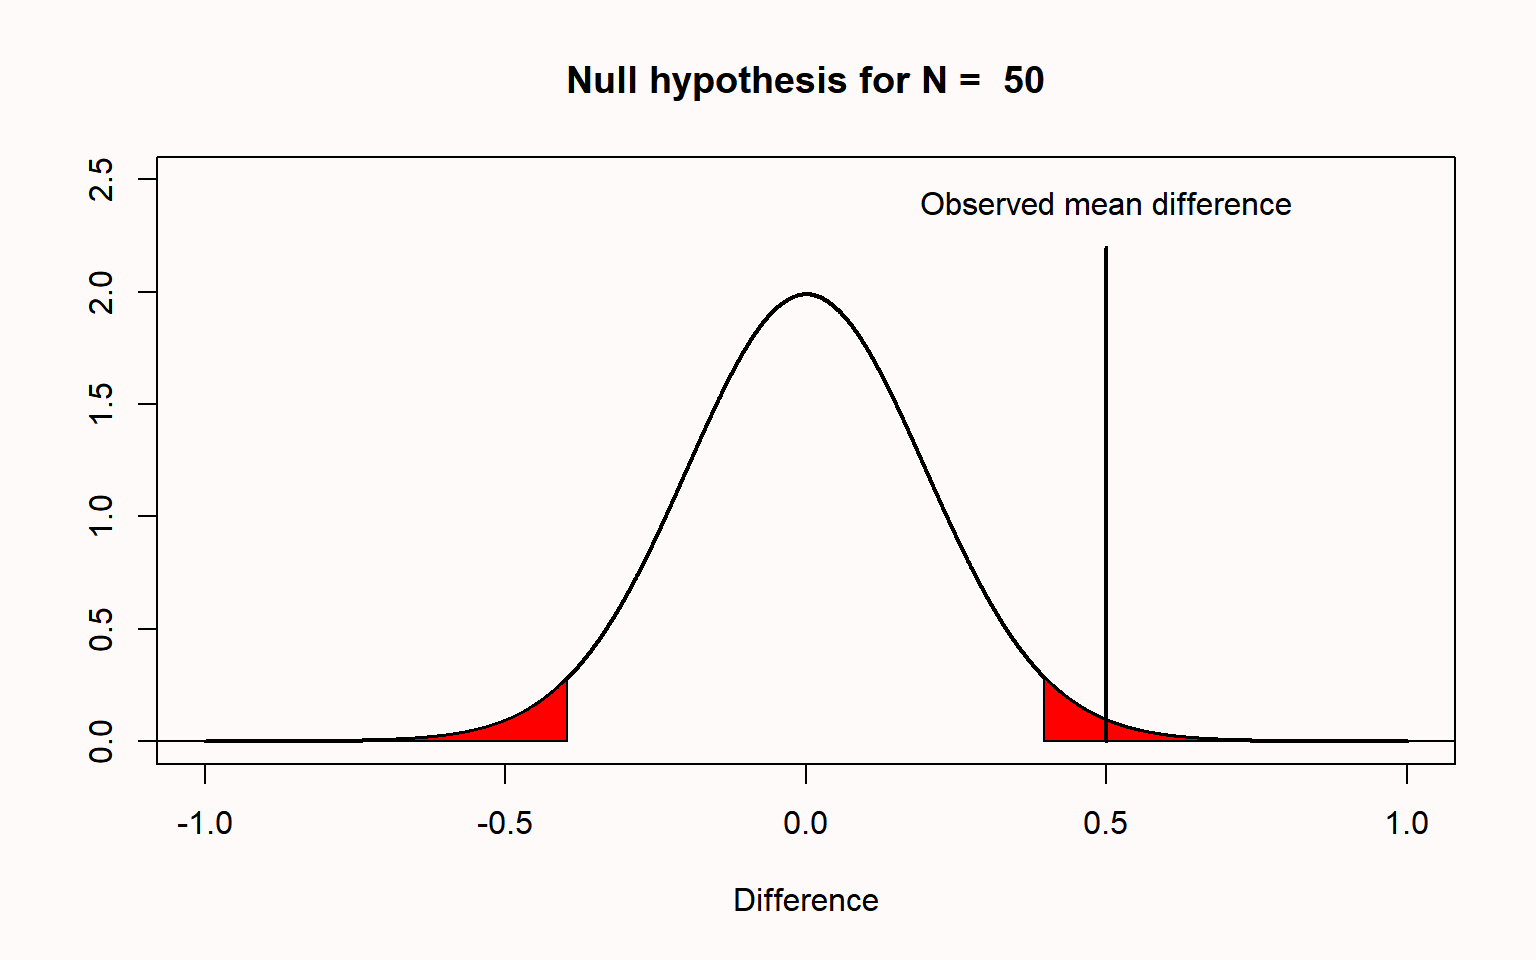
\includegraphics[width=1\linewidth]{01-pvalue_files/figure-latex/fig137-1} 

}

\caption{Distribution of observed Cohen's \emph{d} effect sizes when collecting 50 observations per group in an independent \emph{t}-test when \emph{d} = 0 and observing \emph{d} = 0.5.}\label{fig:fig137}
\end{figure}

The significant \emph{p}-value does not allow us to conclude that the null hypothesis (``the random number generator works'') is false. It is true that the mean of the 50 samples we generated was surprisingly extreme. But a low \emph{p}-value simply tells us that an observation is surprising. We should observe such surprising observations with a low probability when the null hypothesis is true -- when the null is true, they still happen. Therefore, a significant result does not mean an alternative hypothesis is true -- the result can also be a Type 1 error, and in the example above, Omniscient Jones knows that this is the case.

Let's revisit the incorrect statement `\emph{p} \textless{} .05, therefore there is an effect'. A correct interpretation of a significant \emph{p}-value requires us to acknowledge the possibility that our significant result might be a Type 1 error. Remember that Fisher would conclude that ``Either an exceptionally rare chance has occurred, or the theory of random distribution is not true''. A correct interpretation in terms of Neyman-Pearson statistics would be: ``we can act as if the null hypothesis is false, and we would not be wrong more than 5\% of the time in the long run''. Note the specific use of the word `act', which does not imply anything about whether this specific hypothesis is true or false, but merely states that if we act as if the null hypothesis is false any time we observe \emph{p} \textless{} alpha, we will not make an error more than alpha percent of the time.

Both these formally correct statements are a bit long. In scientific articles, we often read a shorter statement such as: `we can reject the null hypothesis', or `we can accept the alternative hypothesis'. These statements might be made with the assumption that readers will themselves add `with a 5\% probability of being wrong, in the long run'. But it might be useful to add `with a 5\% long run error rate' at least the first time you make such a statement in your article to remind readers.

In the example above we have a very strong subjective prior probability that the random number generator in R works. Alternative statistical procedures to incorporate such prior beliefs are \protect\hyperlink{bayes}{Bayesian statistics} or \protect\hyperlink{ppv}{false positive report probabilities}. In frequentist statistics, the idea is that you need to replicate your study several times. You will observe a Type 1 error every now and then, but you are unlikely to observe a Type 1 error three times in a row. Alternatively, you can lower the alpha level in a single study to reduce the probability of a Type 1 error rate.

\hypertarget{misunderstanding-3-a-significant-p-value-means-that-a-practically-important-effect-has-been-discovered.}{%
\subsection{\texorpdfstring{Misunderstanding 3: A significant \emph{p}-value means that a practically important effect has been discovered.}{Misunderstanding 3: A significant p-value means that a practically important effect has been discovered.}}\label{misunderstanding-3-a-significant-p-value-means-that-a-practically-important-effect-has-been-discovered.}}

A common concern when interpreting \emph{p}-values is that `significant' in normal language implies `important', and thus a `significant' effect is interpreted as an `important' effect. However, the question whether an effect is important is completely orthogonal to the question whether it is different from zero, or even how large the effect is. Not all effects have practical impact. The smaller the effect, the less likely such effects will be noticed by individuals, but such effects might still have a large impact on a societal level. Therefore, the general take home message is that statistical significance does not answer the question whether an effect matters in practice, or is `practically important'. To answer the question whether an effect matters, you need to present a cost-benefit analysis.

This issue of practical significance most often comes up in studies with a very large sample size. As we have seen before, with an increasing sample size, the width of the density distribution around the null value becomes more and more narrow, and the values that are considered surprising fall closer and closer to zero.

If we plot the null model for a very large sample size (e.g., n = 10000 per group) we see that even very small mean differences (differences more extreme than a mean difference of 0.04) will be considered `surprising'. This still means that if there really is no difference in the population, you will observe differences larger than 0.04 less than 5\% of the time, in the long run, and 95\% of the observed differences will be smaller than a mean difference of 0.04. But it becomes more difficult to argue for the practical significance of such effects. Imagine that a specific intervention is successful in changing people's spending behavior, and when implementing some intervention people save 12 cents per year. It is difficult to argue how this effect will make any individual happier. However, if this money is combined, it will yield over 2 million, which could be used to treat diseases in developing countries, where it would have a real impact. The cost of the intervention might be considered too high if the goal is to make individuals happier, but it might be consider worthwhile if the goal is to raise 2 million for charity.

Not all effects in psychology are additive (we cannot combine or transfer an increase in happiness of 0.04 scale points), so it is often more difficult to argue for the importance of small effects in subjective feelings \citep{anvari_not_2021}. A cost-benefit analysis might show small effects matter a lot, but whether or not this is the case cannot be inferred from a \emph{p}-value.

Note that nothing about this is a problem with the interpretation of a \emph{p}-value per se: A \emph{p} \textless{} 0.05 still correctly indicates that, if the null hypothesis is true, we have observed data that should be considered surprising. However, just because data is surprising, does not mean we need to care about it. It is mainly the verbal label `significant' that causes confusion here -- it is perhaps less confusing to think of a `significant' effect as a `surprising' effect, but not necessarily as an `important' effect.

\hypertarget{misconception4}{%
\subsection{Misunderstanding 4: If you have observed a significant finding, the probability that you have made a Type 1 error (a false positive) is 5\%.}\label{misconception4}}

This misinterpretation is one possible explanation of the incorrect statement that a \emph{p}-value is `the probability that the data are observed by chance.' Assume we collect 20 observations, and Omniscient Jones tells us the null hypothesis is true (as in the example above where we generated random numbers in R). This means we are sampling from the distribution in the figure below.



\begin{figure}

{\centering 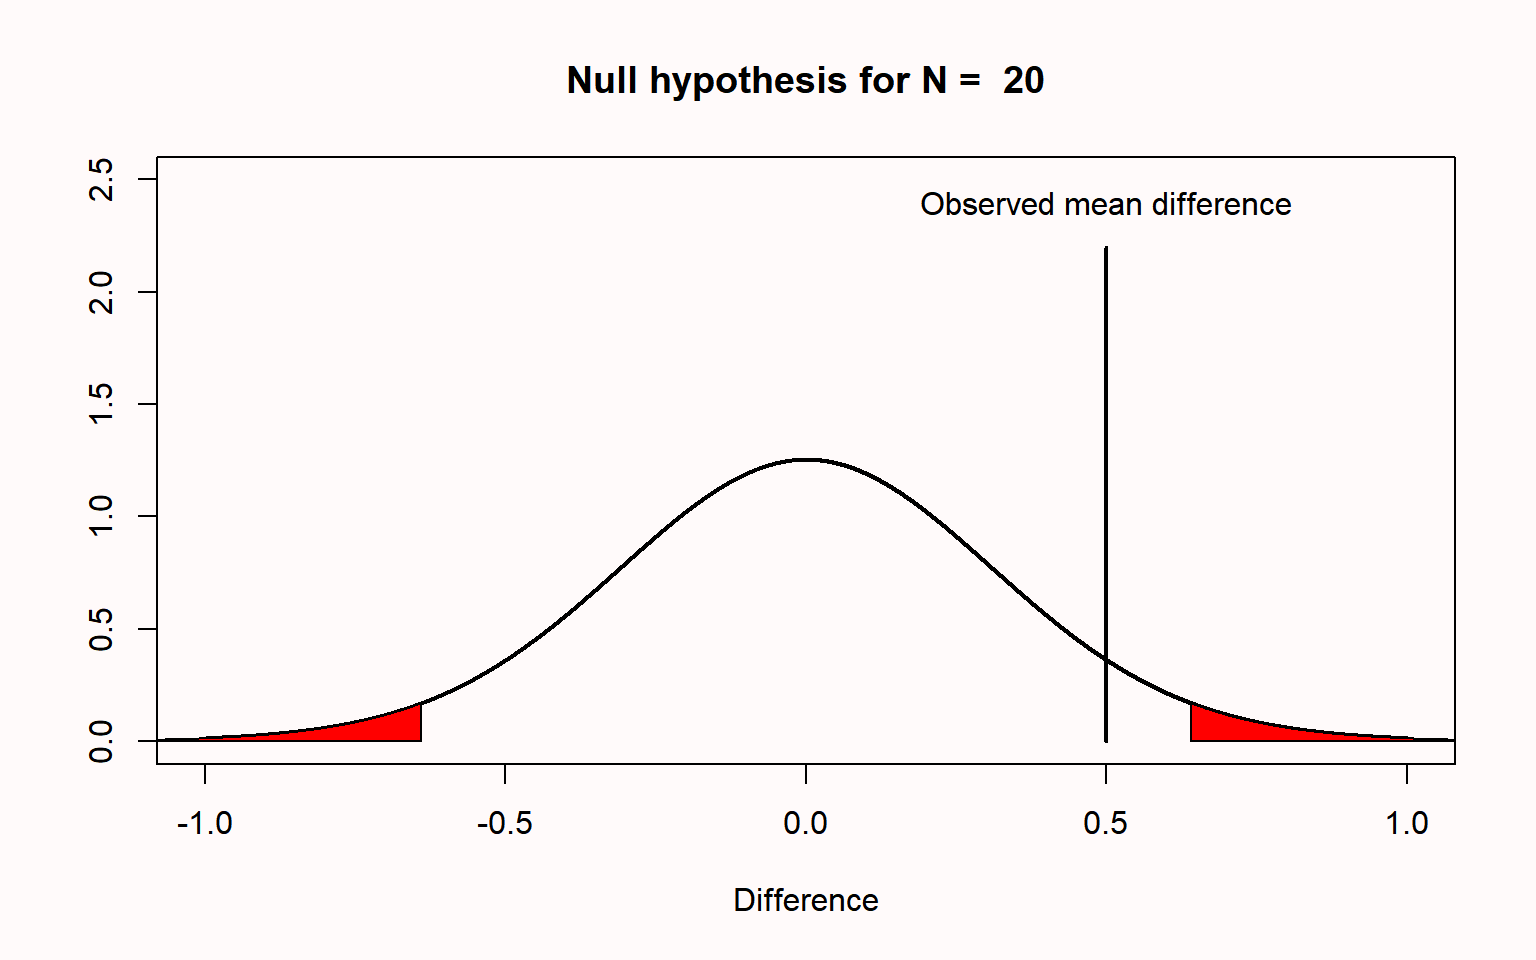
\includegraphics[width=1\linewidth]{01-pvalue_files/figure-latex/fig138-1} 

}

\caption{Distribution of observed Cohen's \emph{d} effect sizes when collecting 20 observations per group in an independent \emph{t}-test when \emph{d} = 0.}\label{fig:fig138}
\end{figure}

If this is our reality, it means that 100\% of the time that we observe a significant result, it is a false positive (or Type I error). Thus, 100\% of our significant results are Type 1 errors.

It is important to distinguish probabilities before collecting the data and analyzing the result, and probabilities after collecting data and analyzing the results. What the Type 1 error rate controls is that from all studies we will perform in the future where the null hypothesis is true, not more than 5\% of our observed mean differences will fall in the red tail areas. But after we have seen that our data falls in the tail areas with \emph{p} \textless{} alpha, and we know that the null hypothesis is true, these observed significant effects are always a Type 1 error. If you read carefully, you will notice that this misunderstanding is cause by differences in the question that is asked. ``If I have observed a \emph{p} \textless{} .05, what is the probability that the null hypothesis is true?'' is a different question than ``If the null hypothesis is true, what is the probability of observing this (or more extreme) data?''. Only the latter question is answered by a \emph{p}-value. The first question cannot be answered without making a subjective judgment about the probability that the null hypothesis is true prior to collecting the data.

\hypertarget{misunderstanding-5-one-minus-the-p-value-is-the-probability-that-the-effect-will-replicate-when-repeated.}{%
\subsection{\texorpdfstring{Misunderstanding 5: One minus the \emph{p}-value is the probability that the effect will replicate when repeated.}{Misunderstanding 5: One minus the p-value is the probability that the effect will replicate when repeated.}}\label{misunderstanding-5-one-minus-the-p-value-is-the-probability-that-the-effect-will-replicate-when-repeated.}}

It is impossible to calculate the probability that an effect will replicate, based on only the \emph{p}-value. The main reason for this is that we do not know the true mean difference. If we were Omniscient Jones, and we knew the true mean difference (e.g., a difference between the two groups of 0.5 scale points) we would know the statistical power of our test. The statistical power is the probability that we will find a significant result, if the alternative model is true (i.e.~if there is a true effect). For example, reading the text in the left bar in the app, we see that with N = 50 per group, alpha level of 0.05, and a true mean difference of 0.5, the probability of finding a significant result (or the statistical power) is 69.69\%. If we would observe a significant effect in this scenario (e.g., \emph{p} = 0.03) it is not true that there is a 97\% probability that an exact replication of the study (with the same sample size) would again yield a significant effect. The probability that a study yields a significant effect is determined by the statistical power - not by the \emph{p}-value in a previous study.

What we can generally take away from this last misunderstanding is the fact that the probability of replication depends on the presence versus the absence of a true effect. In other words, as stated above, if a true effect exists then the level of statistical power informs us about how frequently we should observe a significant result (e.g., 80\% power means we should observe significant result 80\% of the time). On the other hand, if the null hypothesis is true (e.g., the effect is 0) then significant results will be observed only with a frequency approaching the chosen alpha level in the long run (i.e.~a 5\% Type 1 error rate if an an alpha of 0.05 is chosen). Therefore, if the original study correctly observed an effect, the probability of a significant result in a replication study is determined by the statistical power, and if the original study correctly observed no significant effect, the probability of a significant effect in a replication study is determined by the alpha level.

\hypertarget{test-yourself}{%
\section{Test Yourself}\label{test-yourself}}

\hypertarget{questions-about-which-p-values-you-can-expect}{%
\subsection{\texorpdfstring{Questions about which \emph{p}-values you can expect}{Questions about which p-values you can expect}}\label{questions-about-which-p-values-you-can-expect}}

Copy the code below to R and run the code. You can click the `clipboard' icon on the top right of the code section to copy all the code to your clipboard, so you can easily paste it into R.

\begin{Shaded}
\begin{Highlighting}[]
\NormalTok{nsims }\OtherTok{\textless{}{-}} \DecValTok{100000} \CommentTok{\# number of simulations}

\NormalTok{m }\OtherTok{\textless{}{-}} \DecValTok{106} \CommentTok{\# mean sample}
\NormalTok{n }\OtherTok{\textless{}{-}} \DecValTok{26} \CommentTok{\# set sample size}
\NormalTok{sd }\OtherTok{\textless{}{-}} \DecValTok{15} \CommentTok{\# SD of the simulated data}

\NormalTok{p }\OtherTok{\textless{}{-}} \FunctionTok{numeric}\NormalTok{(nsims) }\CommentTok{\# set up empty vector}
\NormalTok{bars }\OtherTok{\textless{}{-}} \DecValTok{20}

\ControlFlowTok{for}\NormalTok{ (i }\ControlFlowTok{in} \DecValTok{1}\SpecialCharTok{:}\NormalTok{nsims) \{ }\CommentTok{\# for each simulated experiment}
\NormalTok{  x }\OtherTok{\textless{}{-}} \FunctionTok{rnorm}\NormalTok{(}\AttributeTok{n =}\NormalTok{ n, }\AttributeTok{mean =}\NormalTok{ m, }\AttributeTok{sd =}\NormalTok{ sd)}
\NormalTok{  z }\OtherTok{\textless{}{-}} \FunctionTok{t.test}\NormalTok{(x, }\AttributeTok{mu =} \DecValTok{100}\NormalTok{) }\CommentTok{\# perform the t{-}test}
\NormalTok{  p[i] }\OtherTok{\textless{}{-}}\NormalTok{ z}\SpecialCharTok{$}\NormalTok{p.value }\CommentTok{\# get the p{-}value}
\NormalTok{\}}
\NormalTok{power }\OtherTok{\textless{}{-}} \FunctionTok{round}\NormalTok{((}\FunctionTok{sum}\NormalTok{(p }\SpecialCharTok{\textless{}} \FloatTok{0.05}\NormalTok{) }\SpecialCharTok{/}\NormalTok{ nsims), }\DecValTok{2}\NormalTok{) }\CommentTok{\# power}

\CommentTok{\# Plot figure}
\FunctionTok{hist}\NormalTok{(p,}
  \AttributeTok{breaks =}\NormalTok{ bars, }\AttributeTok{xlab =} \StringTok{"P{-}values"}\NormalTok{, }\AttributeTok{ylab =} \StringTok{"number of p{-}values}\SpecialCharTok{\textbackslash{}n}\StringTok{"}\NormalTok{, }
  \AttributeTok{axes =} \ConstantTok{FALSE}\NormalTok{,  }\AttributeTok{main =} \FunctionTok{paste}\NormalTok{(}\StringTok{"P{-}value Distribution with"}\NormalTok{, }
                              \FunctionTok{round}\NormalTok{(power }\SpecialCharTok{*} \DecValTok{100}\NormalTok{, }\AttributeTok{digits =} \DecValTok{1}\NormalTok{), }\StringTok{"\% Power"}\NormalTok{),}
  \AttributeTok{col =} \StringTok{"grey"}\NormalTok{, }\AttributeTok{xlim =} \FunctionTok{c}\NormalTok{(}\DecValTok{0}\NormalTok{, }\DecValTok{1}\NormalTok{), }\AttributeTok{ylim =} \FunctionTok{c}\NormalTok{(}\DecValTok{0}\NormalTok{, nsims))}
\FunctionTok{axis}\NormalTok{(}\AttributeTok{side =} \DecValTok{1}\NormalTok{, }\AttributeTok{at =} \FunctionTok{seq}\NormalTok{(}\DecValTok{0}\NormalTok{, }\DecValTok{1}\NormalTok{, }\FloatTok{0.1}\NormalTok{), }\AttributeTok{labels =} \FunctionTok{seq}\NormalTok{(}\DecValTok{0}\NormalTok{, }\DecValTok{1}\NormalTok{, }\FloatTok{0.1}\NormalTok{))}
\FunctionTok{axis}\NormalTok{(}\AttributeTok{side =} \DecValTok{2}\NormalTok{, }\AttributeTok{at =} \FunctionTok{seq}\NormalTok{(}\DecValTok{0}\NormalTok{, nsims, nsims }\SpecialCharTok{/} \DecValTok{4}\NormalTok{), }
     \AttributeTok{labels =} \FunctionTok{seq}\NormalTok{(}\DecValTok{0}\NormalTok{, nsims, nsims }\SpecialCharTok{/} \DecValTok{4}\NormalTok{), }\AttributeTok{las =} \DecValTok{2}\NormalTok{)}
\FunctionTok{abline}\NormalTok{(}\AttributeTok{h =}\NormalTok{ nsims }\SpecialCharTok{/}\NormalTok{ bars, }\AttributeTok{col =} \StringTok{"red"}\NormalTok{, }\AttributeTok{lty =} \DecValTok{3}\NormalTok{)}
\end{Highlighting}
\end{Shaded}

\begin{center}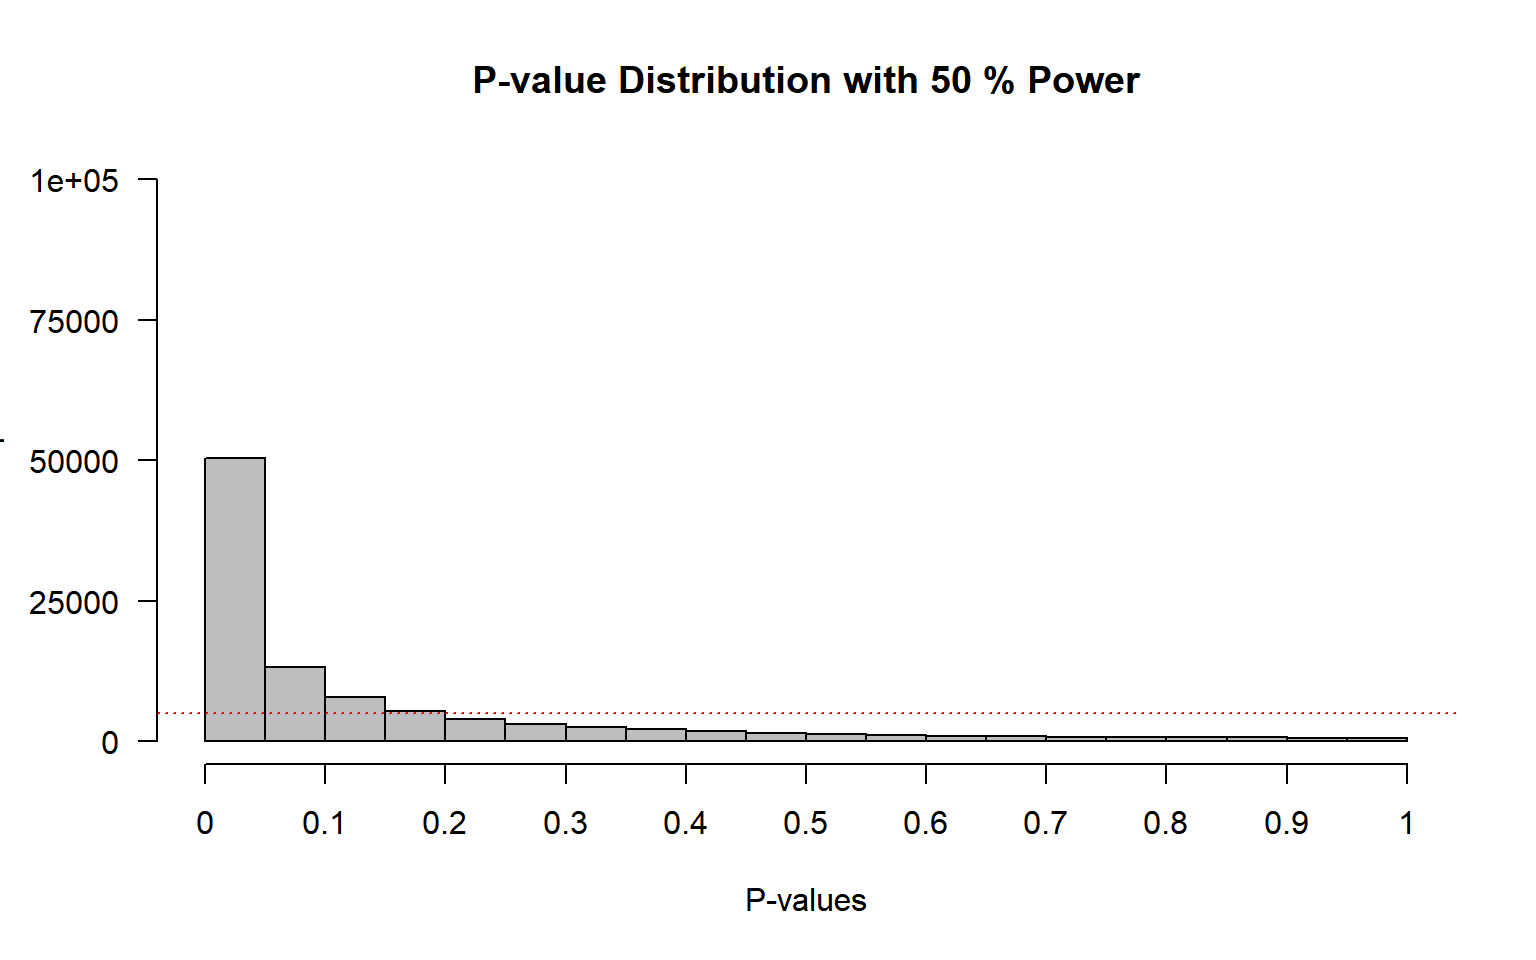
\includegraphics[width=1\linewidth]{01-pvalue_files/figure-latex/q1-1} \end{center}

On the x-axis we see \emph{p}-values from 0 to 1 in 20 bars, and on the y-axis we see how frequently these \emph{p}-values were observed. There is a horizontal red dotted line that indicates an alpha of 5\% (located at a frequency of 100.000*0.05 = 5000) -- but you can ignore this line for now. In the title of the graph, the statistical power that is achieved in the simulated studies is given (assuming an alpha of 0.05): The studies have 50\% power (with minor variations for each simulation).

\textbf{Q1}: Since the statistical power is the probability of observing a statistically significant result, if there is a true effect, we can also see the power in the figure itself. Where?

\begin{enumerate}
\def\labelenumi{\Alph{enumi})}
\tightlist
\item
  We can calculate the number of \emph{p}-values larger than 0.5, and divide them by the number of simulations.
\item
  We can calculate the number of \emph{p}-values in the first bar (which contains all `significant' \emph{p}-values from 0.00 to 0.05) and divide the \emph{p}-values in this bar by the total number of simulations.
\item
  We can calculate the difference between \emph{p}-values above 0.5 minus the \emph{p}-values below 0.5, and divide this number by the total number of simulations.
\item
  We can calculate the difference between \emph{p}-values above 0.5 minus the \emph{p}-values below 0.05, and divide this number by the number of simulations.
\end{enumerate}

\textbf{Q2}: Change the sample size from n \textless- 26 to n \textless- 51. Run the simulation by selecting all lines and pressing CTRL+Enter. What is the power in the simulation now that we have increased the sample size from 26 people to 51 people?

\begin{enumerate}
\def\labelenumi{\Alph{enumi})}
\tightlist
\item
  55\%
\item
  60\%
\item
  80\%
\item
  95\%
\end{enumerate}

\textbf{Q3}: If you look at the distribution of \emph{p}-values, what do you notice?

\begin{enumerate}
\def\labelenumi{\Alph{enumi})}
\tightlist
\item
  The \emph{p}-value distribution is exactly the same as with 50\% power
\item
  The \emph{p}-value distribution is much steeper than with 50\% power
\item
  The \emph{p}-value distribution is much flatter than with 50\% power
\item
  The \emph{p}-value distribution is much more normally distributed than with 50\% power
\end{enumerate}

Feel free to increase and decrease the sample size and see what happens if you run the simulation. When you are done exploring, make sure that n \textless- 51 again.

\textbf{Q4}: What would happen when there is no true difference between our simulated samples and the average IQ score? In this situation, we have no probability to observe an effect, so you might say we have `0 power'. Formally, power is not defined when there is no true effect. However, we can casually refer to this as 0 power. Change the mean in the sample to 100 (set m \textless- 106 to m \textless- 100) There is now no difference between the mean in our sample, and the population value we are testing against in the one-sample \emph{t}-test. Run the script again. What do you notice?

\begin{enumerate}
\def\labelenumi{\Alph{enumi})}
\tightlist
\item
  The \emph{p}-value distribution is exactly the same as with 50\% power
\item
  The \emph{p}-value distribution is much steeper than with 50\% power
\item
  The \emph{p}-value distribution is basically completely flat (ignoring some minor variation due to random noise in the simulation)
\item
  The \emph{p}-value distribution is normally distributed
\end{enumerate}

The question below builds on the simulation above where there was no true difference between the groups.

\textbf{Q5}: Look at the leftmost bar in the plot produced for Q4, and look at the frequency of \emph{p}-values in this bar. What is the formal name for this bar?

\begin{enumerate}
\def\labelenumi{\Alph{enumi})}
\tightlist
\item
  The power (or true positives)
\item
  The true negatives
\item
  The Type 1 error (or false positives)
\item
  The Type 2 error (or false negatives)
\end{enumerate}

Let's take a look at just the \emph{p}-values below 0.05. Bear with me for the next few steps -- it will be worth it. Find the variable that determines how many bars there are, in the statement bars \textless- 20. Change it to bars \textless- 100. We will now get 1 bar for \emph{p}-values between 0 and 0.01, one bar for \emph{p}-values between 0.01 and 0.02, and 100 bars in total. The red dotted line will now indicate the frequency of \emph{p}-values when the null hypothesis is true, where every bar contains 1\% of the total number of \emph{p}-values. We only want to look at \emph{p}-values below 0.05, and we will cut off the plot at 0.05. Change xlim = c(0, 1) to xlim = c(0, 0.05). Instead of seeing all \emph{p}-values between 0 and 1, we will only see \emph{p}-values between 0 and 0.05. Re-run the simulation (still with m \textless- 100). We see the same uniform distribution, but now every bar contains 1\% of the \emph{p}-values, so the \emph{p}-value distribution is very flat and almost impossible to see (we will zoom in on the y-axis later this assignment). The red line now clearly gives the frequency for each bar, assuming the null hypothesis is true.

Change the mean in the simulation in line 9 to m \textless- 107 (remember n is still 51). Re-run the simulation. It's clear we have very high power. Most \emph{p}-values are in the left-most bar, which contains all \emph{p}-values between 0.00 and 0.01.

\textbf{Q6}: The plot from the last simulation tells you we have 90.5\% power. This is the power if we use an alpha of 5\%. But we can also use an alpha of 1\%. What is the statistical power we have in the simulated studies when we would use an alpha of 1\%, looking at the graph? Pick the answer closest to the answer from your simulations.

\begin{enumerate}
\def\labelenumi{\Alph{enumi})}
\tightlist
\item
  \textasciitilde90\%
\item
  \textasciitilde75\%
\item
  \textasciitilde50\%
\item
  \textasciitilde5\%
\end{enumerate}

To be able to look at the \emph{p}-values around 0.03 and 0.04, we will zoom in on the y-axis as well. In the part of the code where the plot is draw, change ylim = c(0, nSims) to ylim = c(0, 10000). Re-run the script.

Change the mean in the sample to 108 in m \textless- 108), and leave the sample size at 51. Run the simulation. Look at how the distribution has changed compared to the graph above.

Look at the fifth bar from the left. This bar now contains all the \emph{p}-values between 0.04 and 0.05. You will notice something peculiar. Remember that the red dotted line indicates the frequency in each bar, assuming the null hypothesis is true. See how the bar with \emph{p}-values between 0.04 and 0.05 is lower than the red line. We have simulated studies with 96\% power. When power is very high, \emph{p}-values between 0.04 and 0.05 are very rare -- they occur less than 1\% of the time (most \emph{p}-values are smaller than 0.01). When the null hypothesis is true, \emph{p}-values between 0.04 and 0.05 occur exactly 1\% of the time (because \emph{p}-values are uniformly distributed). Now ask yourself: When you have very high power, and you observe a \emph{p}-value between 0.04 and 0.05, is it more likely that the null hypothesis is true, or that the alternative hypothesis is true? Given that you are more likely to observe \emph{p}-values between 0.04 and 0.05 when the null hypothesis is true, than when the alternative hypothesis is true, you should interpret a \emph{p}-value significant with an alpha of 0.05 as more likely when the null hypothesis is true, than when the alternative hypothesis is true.

In our simulations, we know there is a true effect or not, but in the real world, you don't know. When you have very high power, use an alpha level of 0.05, and find a \emph{p}-value of \emph{p} = .045, the data is surprising, assuming the null hypothesis is true, but it is even \emph{more} surprising, assuming the alternative hypothesis is true. This shows how a significant \emph{p}-value is not always evidence for the alternative hypothesis.

\textbf{Q7}: When you know you have very high (e.g., 98\%) power for the smallest effect size you care about, and you observe a \emph{p}-value of 0.045, what is the correct conclusion?

\begin{enumerate}
\def\labelenumi{\Alph{enumi})}
\tightlist
\item
  The effect is significant, and provides strong support for the alternative hypothesis.
\item
  The effect is significant, but it is without any doubt a Type 1 error.
\item
  With high power, you should use an alpha level that is smaller than 0.05, and therefore, this effect cannot be considered significant.
\item
  The effect is significant, but the data are more likely under the null hypothesis than under the alternative hypothesis.
\end{enumerate}

\textbf{Q8}: Play around with the sample size (n) and the mean (m) by changing the numerical values or both (and thus, vary the statistical power in the simulated studies). Look at the simulation result for the bar that contains \emph{p}-values between 0.04 and 0.05. The red line indicates how many \emph{p}-values would be found in this bar if the null hypothesis was true (and is always at 1\%). At the very best, how much more likely is a \emph{p}-value between 0.04 and 0.05 to come from a \emph{p}-value distribution representing a true effect, than it is to come from a \emph{p}-value distribution when there is no effect? You can answer this question by seeing how much higher the bar of \emph{p}-values between 0.04 and 0.05 can become. If at best the bar in the simulation is five times as high at the red line (so the bar shows 5\% of \emph{p}-values end up between 0.04 and 0.05, while the red line remains at 1\%), then at best \emph{p}-values between 0.04 and 0.05 are five times as likely when there is a true effect than when there is no true effect.

\begin{enumerate}
\def\labelenumi{\Alph{enumi})}
\tightlist
\item
  At best, \emph{p}-values between 0.04 and 0.05 are equally likely under the
  alternative hypothesis, and under the null hypothesis.
\item
  At best, \emph{p}-values between 0.04 and 0.05 are approximately 4 times more
  likely under the alternative hypothesis, than under the null hypothesis.
\item
  At best, \emph{p}-values between 0.04 and 0.05 are \textasciitilde10 times more likely under the alternative hypothesis, than under the null hypothesis.
\item
  At best, \emph{p}-values between 0.04 and 0.05 are \textasciitilde30 times more likely under the alternative hypothesis, than under the null hypothesis.
\end{enumerate}

For this reason, statisticians warn that \emph{p}-values just below 0.05 (e.g.,
between 0.04 and 0.05) are at the very best weak support for the alternative
hypothesis. If you find \emph{p}-values in this range, consider replicating the
study, or if that's not possible, interpret the result at least a bit
cautiously.

\hypertarget{questions-about-p-value-misconceptions}{%
\subsection{\texorpdfstring{Questions about \emph{p}-value misconceptions}{Questions about p-value misconceptions}}\label{questions-about-p-value-misconceptions}}

\textbf{Q1}: When the sample size in each group of an independent \emph{t}-test is 50
observations (see Figure \ref{fig:fig131}), which statement is correct?

\begin{enumerate}
\def\labelenumi{\Alph{enumi})}
\tightlist
\item
  The mean of the differences you will observe between the two groups is always 0.
\item
  The mean of the differences you will observe between the two groups is always different from 0.
\item
  Observing a mean difference of +0.5 or -0.5 is considered surprising, assuming the null hypothesis is true.
\item
  Observing a mean difference of +0.1 or -0.1 is considered surprising, assuming the null hypothesis is true.
\end{enumerate}

\textbf{Q2:} In what sense are the null models in the figures (Figure \ref{fig:fig131} and \ref{fig:fig132}) similar, and in what sense are they different?

\begin{enumerate}
\def\labelenumi{\Alph{enumi})}
\tightlist
\item
  In both cases, the distributions are centered on zero, and the critical
  \emph{t}-value is between 1.96 and 2 (for a two-sided test, depending on the sample size). But the larger the sample size, the closer to 0 the mean differences fall that are considered `surprising'.
\item
  In both cases, a \emph{t}-value of 0 is the most likely outcome, but the critical \emph{t}-value is around 0.4 for n = 50, and around 0.05 for n = 5000.
\item
  In both cases, means will vary in exactly the same way around 0, but the Type 1 error rate is much smaller when n = 5000 than when n = 50.
\item
  Because the standard error is much larger for n = 50 than for n = 5000, it is much more likely that the null hypothesis is true for n = 50.
\end{enumerate}

\textbf{Q3:} You can play around with the alternative and null models in this online app: \url{http://shiny.ieis.tue.nl/d_p_power/}. The app allows you to specify the sample size in each group of an independent \emph{t}-test (from 2 to infinity), the mean difference (from 0 to 2), and the alpha level. In the plot, the red areas visualize Type 1 errors. The blue area visualizes the Type 2 error rate. The app also tells you the critical value: There is a vertical line (with n = 50 this line falls at a mean difference of 0.4) and a verbal label that says: ``Effects larger than 0.4 will be statistically significant''. Note that the same is true for effects smaller than -0.4, even though there is no second label there, but the app shows the situation for a two-sided independent \emph{t}-test.

You can see that on the left of the vertical line that indicates the critical mean difference there is a blue area that is part of the alternative model. This is the Type 2 error rate (or 1 - the power of the study). If a study has 80\% power, 80\% of the mean differences we will observe should fall on the right of the critical value indicated by the line. If the alternative model is true, but we observe an effect smaller than the critical value, the observed \emph{p}-value will be larger than 0.05, even when there is a true effect. You can check in the app that the larger the effect size, the further to the right the entire alternative distribution falls, and thus the higher the power. You can also see that the larger the sample size, the narrower the distribution, and the less of the distribution will fall below the critical value (as long as the true population mean is larger than the critical value). Finally, the larger the alpha level, the further to the left the critical mean difference moves, and the smaller the area of the alternative distribution that falls below the critical value.

The app also plots 3 graphs that illustrate the power curves as a function of different alpha levels, sample sizes, or true mean differences. Play around in the app by changing the values. Get a feel for how each variable impacts the null and alternative models, the mean difference that will be statistically significant, and the Type 1 and Type 2 error rates.

Open the app, and make sure it is set to the default settings of a sample size of 50 and an alpha level of 0.05. Look at the distribution of the null model. Set the sample size to 2. Set the sample size to 5000. The app will not allow you to plot data for a `group' size of 1, but with n = 2 you will get a pretty good idea of the range of values you can expect when the true effect is 0, and when you collect single observations (n = 1). Given your experiences with the app as you change different parameters, which statement is true?

\begin{enumerate}
\def\labelenumi{\Alph{enumi})}
\tightlist
\item
  When the null hypothesis is true and the standard deviation is 1, if you randomly take 1 observation from each group and calculate the difference score, the differences will fall between -0.4 and 0.4 for 95\% of the pairs of observations you will draw.
\item
  When the null hypothesis is true and the standard deviation is 1, with n = 50 per group, 95\% of studies where data is collected will observe in the long run a mean difference between -0.4 and 0.4.
\item
  In any study with n = 50 per group, even when the SD is unknown and it is not known if the null hypothesis is true, you should rarely observe a mean difference more extreme than -0.4 or 0.4.
\item
  As the sample size increases, the expected distribution of means become narrower for the null model, but not for the alternative model.
\end{enumerate}

\textbf{Q4:} Open the app once more with the default settings. Set the slider for the alpha level to 0.01 (while keeping the mean difference at 0.5 and the sample size at 50). Compared to the critical value when alpha = 0.05, which statement is true?

\begin{enumerate}
\def\labelenumi{\Alph{enumi})}
\tightlist
\item
  Compared to an alpha of 0.05, only \emph{less} extreme values are considered surprising when an alpha of 0.01 is used, and only differences larger than 0.53 scale points (or smaller than -0.53) will now be statistically significant.
\item
  Compared to an alpha of 0.05, only \emph{less} extreme values are considered surprising when an alpha of 0.01 is used, and only differences larger than 0.33 scale points (or smaller than -0.33) will now be statistically significant.
\item
  Compared to an alpha of 0.05, only \emph{more} extreme values are considered surprising when an alpha of 0.01 is used, and only differences larger than 0.53 scale points (or smaller than -0.53) will be statistically significant.
\item
  Compared to an alpha of 0.05, only \emph{more} extreme values are considered surprising when an alpha of 0.01 is used, and only differences larger than 0.33 scale points (or smaller than -0.33) will now be statistically significant.
\end{enumerate}

\textbf{Q5:} Why can't you conclude that the null hypothesis is true, when you observe a statistically non-significant \emph{p}-value (\emph{p} \textgreater{} alpha)?

\begin{enumerate}
\def\labelenumi{\Alph{enumi})}
\tightlist
\item
  When calculating \emph{p}-values you always need to take the prior probability into account.
\item
  You need to acknowledge the probability that you have observed a Type 1 error.
\item
  The null hypothesis is never true.
\item
  You need to acknowledge the probability that you have observed a Type 2 error.
\end{enumerate}

\textbf{Q6:} Why can't you conclude that the alternative hypothesis is true, when you observe a statistically significant \emph{p}-value (\emph{p} \textless{} alpha)?

\begin{enumerate}
\def\labelenumi{\Alph{enumi})}
\tightlist
\item
  When calculating \emph{p}-values you always need to take the prior probability into account.
\item
  You need to acknowledge the probability that you have observed a Type 1 error.
\item
  The alternative hypothesis is never true.
\item
  You need to acknowledge the probability that you have observed a Type 2 error.
\end{enumerate}

\textbf{Q7:} A common concern when interpreting \emph{p}-values is that `significant' in normal language implies `important', and thus a `significant' effect is interpreted as an `important' effect. However, \textbf{the question whether an effect is important is completely orthogonal to the question whether it is different from zero, or even how large the effect is}. Not all effects have practical impact. The smaller the effect, the less likely such effects will be noticed by individuals, but such effects might still have a large impact on a societal level. Therefore, the general take home message is that \textbf{statistical significance does not answer the question whether an effect matters in practice, or is `practically important'}. To answer the question whether an effect matters, you need to present a \textbf{cost-benefit analysis}.

Go to the app: \url{http://shiny.ieis.tue.nl/d_p_power/}. Set the sample size to 50000, the mean difference to 0.5, and the alpha level to 0.05. Which effects will, when observed, be statistically different from 0?

\begin{enumerate}
\def\labelenumi{\Alph{enumi})}
\tightlist
\item
  Effects more extreme than -0.01 and 0.01
\item
  Effects more extreme than -0.04 and 0.04
\item
  Effects more extreme than -0.05 and 0.05
\item
  Effects more extreme than -0.12 and 0.12
\end{enumerate}

If we plot the null model for a very large sample size (e.g., n = 10000 per group) we see that even very small mean differences (differences more extreme than a mean difference of 0.04) will be considered `surprising'. This still means that if there really is no difference in the population, you will observe differences larger than 0.04 less than 5\% of the time, in the long run, and 95\% of the observed differences will be smaller than a mean difference of 0.04. But it becomes more difficult to argue for the practical significance of such effects. Imagine that a specific intervention is successful in changing people's spending behavior, and when implementing some intervention people save 12 cents per year. It is difficult to argue how this effect will make any individual happier. However, if this money is combined, it will yield over 2 million, which could be used to treat diseases in developing countries, where it would have a real impact. The cost of the intervention might be considered too high if the goal is to make individuals happier, but it might be consider worthwhile if the goal is to raise 2 million for charity.

Not all effects in psychology are additive (we cannot combine or transfer an increase in happiness of 0.04 scale points), so it is often more difficult to argue for the importance of small effects in subjective feelings. A cost-benefit analysis might show small effects matter a lot, but whether or not this is the case cannot be inferred from a \emph{p}-value. Instead, you need to report and interpret the \protect\hyperlink{effectsize}{effect size},

\textbf{Q8:} Let's assume that the random number generator in R works, and we use rnorm(n = 50, mean = 0, sd = 1) to generate 50 observations, and the mean of these observations is 0.5, which in a one-sample \emph{t}-test against an effect of 0 yields a \emph{p}-value of 0.03, which is smaller than the alpha level (which we have set to 0.05). What is the probability that we have observed a significant difference (\emph{p} \textless{} alpha) just by chance?

\begin{enumerate}
\def\labelenumi{\Alph{enumi})}
\tightlist
\item
  3\%
\item
  5\%
\item
  95\%
\item
  100\%
\end{enumerate}

\textbf{Q9:} Which statement is true?

\begin{enumerate}
\def\labelenumi{\Alph{enumi})}
\tightlist
\item
  The probability that a replication study will yield a significant result is 1-\emph{p}.
\item
  The probability that a replication study will yield a significant result is 1-\emph{p} multiplied by the probability that the null hypothesis is true.
\item
  The probability that a replication study will yield a significant result is equal to the statistical power of the replication study (if there is a true effect), or the alpha level (if there is no true effect).
\item
  The probability that a replication study will yield a significant result is equal to the statistical power of the replication study + the alpha level.
\end{enumerate}

This question is conceptually very similar to that asked by Tversky and Kahneman \citeyearpar{tversky_belief_1971} in article `Belief in the law of small numbers':



\begin{figure}

{\centering 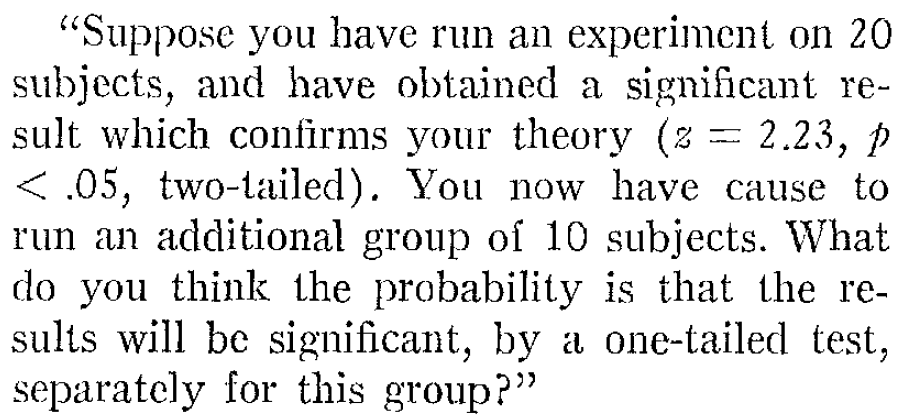
\includegraphics[width=1\linewidth]{images/belieflawsmallnumers} 

}

\caption{Screenshot of first paragraph in Tversky and Kahneman, 1971.}\label{fig:smallnumbers}
\end{figure}

\begin{quote}
Suppose you have run an experiment on 20 subjects, and have obtained a significant result which confirms your theory (\emph{z} = 2.23, \emph{p} \textless{} .05, two-tailed). You now have cause to run an additional group of 10 subjects. What do you think the probability is that the results will be significant, by a one-tailed test, separately for this group?
\end{quote}

Tversky and Kahneman argue a reasonable answer is 48\%, but the only correct response is the same as the correct response to question 9, and the exact probability cannot be known \citep{miller_what_2009}.

\textbf{Q10:} Does a non-significant \emph{p}-value (i.e., \emph{p} = 0.65) mean that the null hypothesis is true?

\begin{enumerate}
\def\labelenumi{\Alph{enumi})}
\tightlist
\item
  No - the result could be a Type 2 error, or a false negative.
\item
  Yes, because it is a true negative.
\item
  Yes, if the \emph{p}-value is larger than the alpha level the null hypothesis is true.
\item
  No, because you need at least two non-significant \emph{p}-values to conclude the null hypothesis is true.
\end{enumerate}

\textbf{Q11:} What is a correct way to present a non-significant \emph{p}-value (e.g., \emph{p} = 0.34 assuming an alpha level of 0.05 is used in an independent \emph{t}-test)?

\begin{enumerate}
\def\labelenumi{\Alph{enumi})}
\tightlist
\item
  The null hypothesis was confirmed, \emph{p} \textgreater{} 0.05
\item
  There was no difference between the two conditions, \emph{p} \textgreater{} 0.05
\item
  The observed difference was not statistically different from 0.
\item
  The null hypothesis is true.
\end{enumerate}

\textbf{Q12:} Does observing a significant \emph{p}-value (\emph{p} \textless{} .05) mean that the null hypothesis is false?

\begin{enumerate}
\def\labelenumi{\Alph{enumi})}
\tightlist
\item
  No, because \emph{p} \textless{} .05 only means that the alternative is true, not that the null hypothesis is wrong.
\item
  No, because \emph{p}-values are never a statement about the probability of a hypothesis or theory.
\item
  Yes, because an exceptionally rare event has occurred.
\item
  Yes, because the difference is statistically significant.
\end{enumerate}

\textbf{Q13:} Is a statistically significant effect always a practically important effect?

\begin{enumerate}
\def\labelenumi{\Alph{enumi})}
\tightlist
\item
  No, because in extremely large samples, extremely small effects can be statistically significant, and small effects are never practically important.
\item
  No, because the alpha level could in theory be set to 0.20, and in that case a significant effect is not practically important.
\item
  No, because how important an effect is depends on a cost-benefit analysis, not on how surprising the data is under the null hypothesis.
\item
  All of the above are true.
\end{enumerate}

\textbf{Q14:} What is the correct definition of a \emph{p}-value?

\begin{enumerate}
\def\labelenumi{\Alph{enumi})}
\tightlist
\item
  A \emph{p}-value is the probability that the null hypothesis is true, given data that is as extreme or more extreme than the data you have observed.
\item
  A \emph{p}-value is the probability that the alternative hypothesis is true, given data that is as extreme or more extreme than the data you have observed.
\item
  A \emph{p}-value is the probability of observing data that is as extreme or more extreme than the data you have observed, assuming the alternative hypothesis is true.
\item
  A \emph{p}-value is the probability of observing data that is as extreme or more extreme than the data you have observed, assuming the null hypothesis is true.
\end{enumerate}

\hypertarget{open-questions}{%
\subsection{Open Questions}\label{open-questions}}

\begin{enumerate}
\def\labelenumi{\arabic{enumi}.}
\item
  What determines the shape of the \emph{p}-value distribution?
\item
  How does the shape of the \emph{p}-value distribution change when there is a true effect and the sample size increases?
\item
  What is Lindley's paradox?
\item
  How are \emph{p}-values distributed when there is no true effect?
\item
  What is the correct definition of a \emph{p}-value?
\item
  Why is it incorrect to think that a non-significant \emph{p}-value means that the null hypothesis is true?
\item
  Why is it incorrect to think that a significant \emph{p}-value means that the null hypothesis is false?
\item
  Why is it incorrect to think that a significant \emph{p}-value means that a practically important effect has been discovered?
\item
  Why is it incorrect to think that if you have observed a significant finding, the probability that you have made a Type 1 error (a false positive) is 5\%?
\item
  Why is it incorrect to think that 1 -- \emph{p} (e.g., 1 -- 0.05 = 0.95) is the probability that the effect will replicate when repeated?
\end{enumerate}

\hypertarget{errorcontrol}{%
\chapter{Error control}\label{errorcontrol}}

In the previous chapter on \protect\hyperlink{pvalue}{\emph{p}-values} we have learned that in the Neyman-Pearson approach to hypothesis testing the goal is to make scientific claims while controlling how often you will make a fool of yourself in the long run. As Benjamini \citeyearpar{benjamini_its_2016} notes, a \emph{p}-value ``offers a first line of defense against being fooled by randomness, separating signal from noise''. There are indications that banning the use of \emph{p}-values increases the ability of researchers to present erroneous claims. Based on qualitative analyses of scientific articles published after the null hypothesis significance ban in the journal Basic and Applied Social Psychology \citet{fricker_assessing_2019} conclude: ``When researchers only employ descriptive statistics we found that they are likely to overinterpret and/or overstate their results compared to a researcher who uses hypothesis testing with the p \textless{} 0.05 threshold''. Researchers often do not control error rates when they make claims, and sometimes intentionally use flexibility in the data analysis to `p-hack' or cherry-pick one out of many performed analyses that shows the results they wanted to see. From an error-statistical approach to statistical inferences, this is problematic behavior, as Mayo \citeyearpar{mayo_statistical_2018} writes:

\begin{quote}
The problem with cherry picking, hunting for significance, and a host of biasing selection effects -- the main source of handwringing behind the statistics crisis in science -- is they wreak havoc with a method's error probabilities. It becomes easy to arrive at findings that have not been severely tested.
\end{quote}

\hypertarget{which-outcome-can-you-expect-if-you-perform-a-study}{%
\section{Which outcome can you expect if you perform a study?}\label{which-outcome-can-you-expect-if-you-perform-a-study}}

If you perform a study and plan to make a claim based on the statistical test you plan to perform, the long run probability of making a correct claim or an erroneous claim is determined by three factors, namely the Type 1 error rate, the Type 2 error rate, and the probability that the null hypothesis is true. There are four possible outcomes of a statistical test, depending on whether the result is statistically significant or not, and whether the null hypothesis is true, or not.

\textbf{False Positive (FP)}: Concluding there is a true effect, when there is a no true effect (\(H_0\) is true). This is also referred to as a \textbf{Type 1 error}, and indicated by \textbf{\(\alpha\)}.

\textbf{False Negative (FN)}: Concluding there is a no true effect, when there is a true effect (\(H_1\) is true). This is also referred to as a \textbf{Type 2 error}, and indicated by \textbf{\(\beta\)}.

\textbf{True Negative (TN)}: Concluding there is no true effect, when there is no true effect (\(H_0\) is true). This is the complement of False Positives, and is thus indicated by \textbf{1-\(\alpha\)}.

\textbf{True Positive (TP)}: Concluding there is a true effect, when there is a true effect (\(H_1\) is true). This is the complement of False Negatives, and is thus indicated by \textbf{1-\(\beta\)}.

The probability of observing a true positive when there is a true effect is, in the long run, equal to the \textbf{statistical power} of your study. The probability of observing a false positive when the null hypothesis is true is, in the long run, equal to the \textbf{alpha level} you have set, or the \textbf{Type 1 error rate}.

\begin{figure}

{\centering 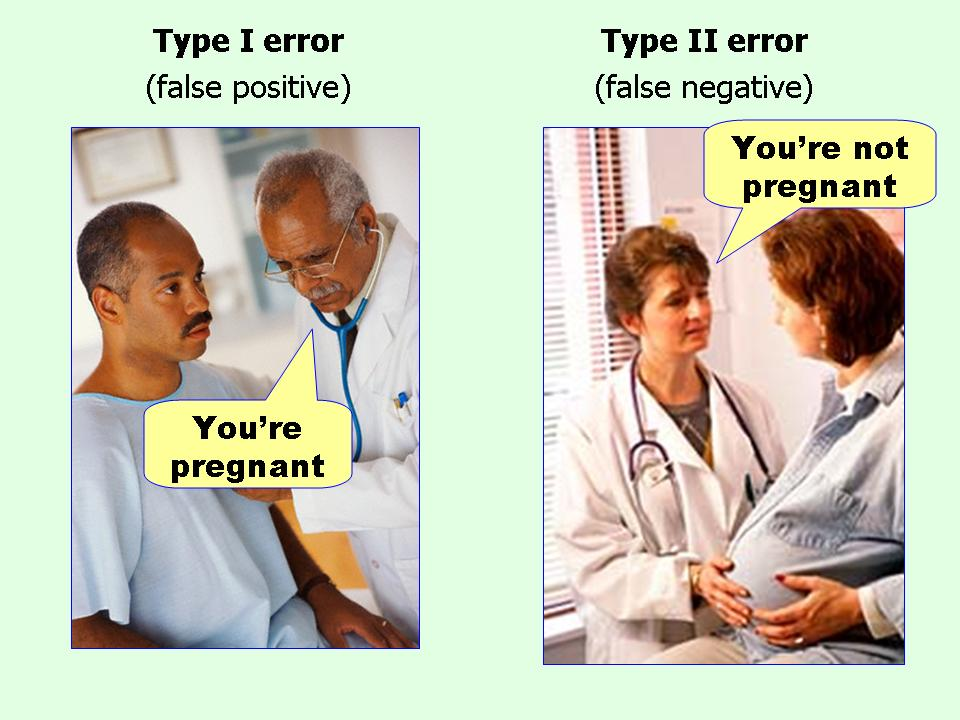
\includegraphics[width=1\linewidth]{images/type1type2error} 

}

\caption{Difference between Type 1 and Type 2 errors. Figure made by <a href="https://effectsizefaq.com/2010/05/31/i-always-get-confused-about-type-i-and-ii-errors-can-you-show-me-something-to-help-me-remember-the-difference/">Paul Ellis</a>}\label{fig:errortypes}
\end{figure}

So, for the next study you will perform, which of the four possible outcomes is most likely? First, let's assume you have set the alpha level to 5\%. Furthermore, let's assume you have designed a study so that it will have 80\% power (and for this example, let's assume Omniscient Jones knows you indeed have exactly 80\% power). The last thing to specify is the probability that the null hypothesis is true. Let's assume for this next study you have no idea if the null hypothesis is true or not, and that it is equally likely that the null hypothesis is true, or the alternative hypothesis is true (both have a probability of 50\%). We can now calculate what the most likely outcome of such a study is.

Before we perform this calculation, take a moment to think if you know the answer. You might have designed studies with a 5\% alpha level and 80\% power, where you believed it was equally likely that \(H_0\) or \(H_1\) was true. Surely, it is useful to have reasonable expectations about which result to expect, when we perform such a study? Yet in my experience, many researchers perform without thinking about these probabilities at all. They often hope to observe a true positive, even when in the situation described above, the most likely outcome is a true negative. Let's now calculate these probabilities.

Let's assume we perform 200 studies with a 5\% alpha level, 80\% power, and a 50\% probability that \(H_0\) is true. How many false positives, true positives, false negatives, and true negatives should we expect in the long run?

\begin{longtable}[]{@{}
  >{\raggedright\arraybackslash}p{(\columnwidth - 4\tabcolsep) * \real{0.3922}}
  >{\raggedright\arraybackslash}p{(\columnwidth - 4\tabcolsep) * \real{0.3072}}
  >{\raggedright\arraybackslash}p{(\columnwidth - 4\tabcolsep) * \real{0.3007}}@{}}
\toprule()
\begin{minipage}[b]{\linewidth}\raggedright
\end{minipage} & \begin{minipage}[b]{\linewidth}\raggedright
\(H_0\) True (50\%)
\end{minipage} & \begin{minipage}[b]{\linewidth}\raggedright
\(H_1\) True (50\%)
\end{minipage} \\
\midrule()
\endhead
Significant Finding (Positive result) \(\alpha\) = 5\%, 1-\(\beta\) = 80\% & \textbf{False Positive 5\% \(\times\) 50\% = 2.5\% (5 studies)} & \textbf{True Positive 80\% \(\times\) 50\% = 40\% (80 studies)} \\
Non-Significant Finding (Negative result) 1-\(\alpha\) = 95\%, \(\beta\) = 20\% & \textbf{True Negative 95\% \(\times\) 50\% = 47.5\% (95 studies)} & \textbf{False Negative 20\% \(\times\) 50\% = 10\% (20 studies)} \\
\bottomrule()
\end{longtable}

In the table above we see that 2.5\% of all studies will be a false positive (a 5\% Type 1 error rate, multiplied by a 50\% probability that \(H_0\) is true). 40\% of all studies will be a true positive (80\% power multiplied by a 50\% probability that \(H_1\) is true). The probability of a false negative is 10\% (a 20\% Type 2 error rate multiplied by a 50\% probability that \(H_1\) is true). The most likely outcome is a true negative, with 47.5\% (a 95\% probability observing a non-significant result, multiplied by a 50\% probability that \(H_0\) is true).

It might be that you are not too enthusiastic about this outlook, and you would like to perform studies that have a higher probability of observing a true positive. What should we do? We can reduce the alpha level, increase the power, or increase the probability that \(H_1\) is true. As the probability of observing a true positive depends on the power, multiplied by the probability that \(H_1\) is true, we should design studies where both of these values are high. Statistical power can be increased by changes in the design of the study (e.g., by increasing the sample size). The probability that \(H_1\) is true depends on the hypothesis you are testing. If the probability that \(H_1\) is true is very high from the outset, you are at the risk of testing a hypothesis that is already established with enough certainty. A solution, which might not happen that often in your career, is to come up with the test of a hypothesis that is not trivial, but that after explaining it to peers makes a lot of sense. In other words, they would not have come up with the idea themselves, but after explaining it to them, they think it is extremely plausible. Such creative research ideas will most likely be very rare in your academic career, if you ever have any at all. Not all research needs to be this ground-breaking. It is also extremely valuable to perform \textbf{replication and extension studies} where it is relatively likely that \(H_1\) is true, but the scientific community still benefits from knowing that findings generalize to different circumstances.

\hypertarget{ppv}{%
\section{Positive predictive value}\label{ppv}}

John Ioannides wrote a well known article titled ``Why Most Published Research Findings Are False'' \citep{ioannidis_why_2005}. At the same time, we have learned that if you set your alpha at 5\%, the Type 1 error rate will not be higher than 5\% (in the long run). How are these two statements related? Why aren't 95\% of published research findings true? They key to understanding this difference is that two different probabilities are calculated. The Type 1 error rate is the probability of saying there is an effect, when there is no effect. Ioannides calculates the \emph{positive predictive value} (PPV), which is the conditional probability that if a study turns out to show a statistically significant result, there is actually a true effect. This probability is useful to understand, because people often selectively focus on significant results, and because due to publication bias, in some research areas only significant results are published.

A real-life example where it was useful to understand the concept of the positive predictive value concerned the number of vaccinated and unvaccinated people admitted to hospital with COVID symptoms. In some places, equal numbers of patients were vaccinated as unvaccinated. If you do not understand the concept of a positive predictive value, you might believe this reveals that it is equally likely to end up in the hospital, whether you are vaccinated or not. This is incorrect. As Figure \ref{fig:ppvhospital} nicely visualizes, the probability that a person is vaccinated is very high, and the probability that a vaccinated person ends up in the hospital is much lower than the probability that an unvaccinated person ends up in the hospital. However, if we select only those individuals who end up in the hospital, we are computing a probability \emph{conditional} on being in the hospital.



\begin{figure}

{\centering 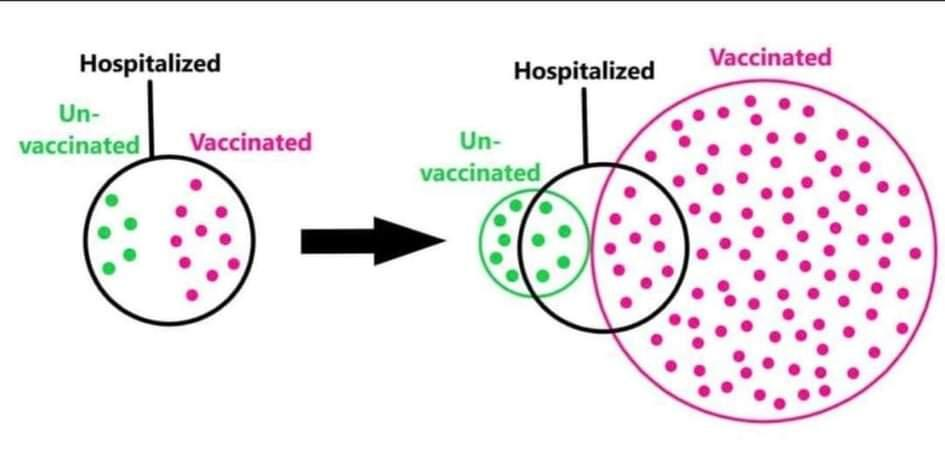
\includegraphics[width=1\linewidth]{images/hospitalvaccinated} 

}

\caption{The positive predictive value can be used to explain why there are more vaccinated people in the hospital than unvaccinated people.}\label{fig:ppvhospital}
\end{figure}

It is useful to understand what the probability is that, if you have observed a significant result in an experiment, the result is actually a true positive. In other words, in the long run, how many \emph{true positives} can we expect, among all positive results (both true positives and false positives)? This is known as the Positive Predictive Value (PPV). We can also calculate how many \emph{false positives} we can expect, among all positive results (again, both true positives and false positives). This is known as the \textbf{False Positive Report Probability} \citep{wacholder_assessing_2004}, sometimes also referred to as the False Positive Risk \citep{colquhoun_false_2019}.

\[PPV = \frac{\text{True}\ \text{Positives}}{(\text{True}\ \text{Positives} +
                                                \text{False}\ \text{Positives})}\]

\[FPRP = \frac{\text{False}\ \text{Positives}}{(\text{True}\ \text{Positives}
                                                  + \text{False}\ \text{Positives})}\]

The PPV and FPRP combine classic Frequentist concepts of statistical power and alpha levels with prior probabilities that \(H_0\) and \(H_1\) are true. They depend on the proportion of studies you do where there is an effect (\(H_1\) is true), and where there is no effect (\(H_0\) is true), in addition to the statistical power, and the alpha level. After all, you can only observe a false positive if the null hypothesis is true, and you can only observe a true positive if the alternative hypothesis is true. Whenever you perform a study, you are either operating in a reality where there is a true effect, or you are operating in a reality where there is no effect -- but you don't know in which reality you are.

When you perform studies, you will be aware of all outcomes of your studies (both the significant and the non-significant findings). When you read the literature, there is publication bias, and you often only have access to significant results. This is when thinking about the PPV (and the FPRP) becomes important. If we set the alpha level to 5\%, in the long run 5\% of studies where \(H_0\) is true (FP + TN) will be significant. But in a literature with only significant results, we do not have access to all true negatives, and it is possible that the proportion of false positives in the literature is much larger than 5\%.

If we continue the example above, we see there are 85 positive results (80 + 5) in the 200 studies. The false positive report probability is 5/85 = 0.0588. At the same time, the alpha of 5\% guarantees that (in the long run) 5\% of the 100 studies where the null hypothesis is true are Type 1 errors: 5\%*100 = 5. This is also true. When we do 200 studies, at most 0.05*200 = 10 could possibly be false positives (if \(H_0\) was true in all experiments). In the 200 studies we performed (and where \(H_0\) was true in only 50\% of the studies), the \textbf{proportion of false positives for all experiments} is only 2.5\%. Thus, for all experiments you do, the proportion of false positives will, in the long run, never be higher than the Type I error rate set by the researcher (e.g., 5\% when \(H_0\) is true in all experiments), but it can be lower (when \(H_0\) is true in less than 100\% of the experiments).

\begin{figure}

{\centering 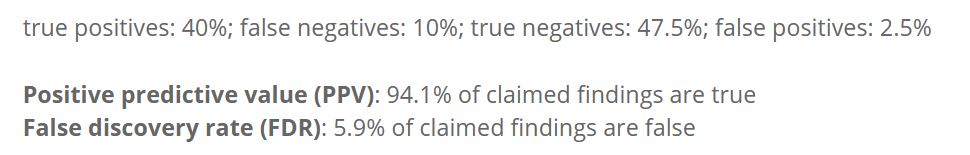
\includegraphics[width=1\linewidth]{images/PPVexample} 

}

\caption{Screenshot of the output of the results of the PPV Shiny app by <a href="http://shinyapps.org/apps/PPV/">Michael Zehetleitner and Felix Schönbrodt </a>}\label{fig:ppvexample}
\end{figure}

\emph{(Note: The FDR and FPRP are different abbreviations for the same thing.)}

People often say something like: ``\emph{Well, we all know 1 in 20 results in the published literature are Type 1 errors}''. You should be able to understand this is not true in practice, after learning about the positive predictive value. When in 100\% of the studies you perform, the null hypothesis is true, and all studies are published, only \emph{then} are 1 in 20 studies, in the long run, false positives (and the rest correctly reveal no statistically significant difference). It also explains why the common \emph{p}-value \protect\hyperlink{misconception4}{misconception} ``If you have observed a significant finding, the probability that you have made a Type 1 error (a false positive) is 5\%.'' is not correct, because in practice the null hypothesis is not true in all tests that are performed (sometimes the alternative hypothesis is true). Importantly, as long as there is \protect\hyperlink{bias}{publication bias} (where findings with desired results end up in the scientific literature, and for example non-significant results are not shared) then even if researchers use a 5\% alpha level, it is quite reasonable to assume much more than 5\% of significant findings in the published literature are false positives. In the scientific literature, the false positive report probability can be quite high, and under specific circumstances, it might even be so high that most published research findings are false. This will happen when researchers examine mostly studies where the null hypothesis is true, with low power, or when the Type 1 error rate is inflated due to \emph{p}-hacking or other types of bias.

\hypertarget{type-1-error-inflation}{%
\section{Type 1 error inflation}\label{type-1-error-inflation}}

\begin{figure}

{\centering 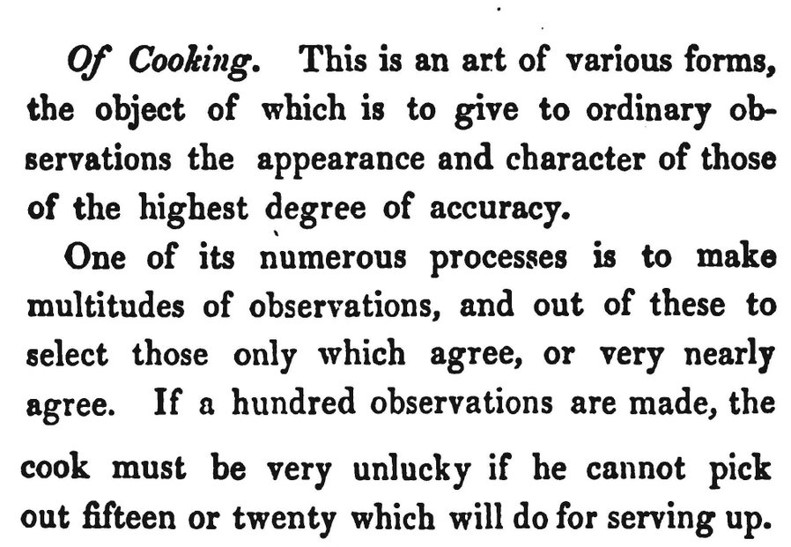
\includegraphics[width=1\linewidth]{images/babbagecooking} 

}

\caption{Quote from the 1830 book by Babbage Reflections on the Decline of Science in England And on Some of Its Causes.}\label{fig:cooking}
\end{figure}

If you perform multiple comparisons, there is a risk that the Type 1 error rate inflates. When multiple comparisons are planned, in some cases it is possible to control the Type 1 error rate by lowering the alpha level for each individual analysis. The most widely known approach to control for multiple comparisons is the Bonferroni correction where the alpha level is divided by the number of tests that is performed \citep{dunn_multiple_1961}. However, researchers also often use informal data analysis strategies that inflate the Type 1 error rate. Babbage \citeyearpar{babbage_reflections_1830} already complained about these problematic practices in 1830, and two centuries later, they are still common. Barber \citeyearpar{barber_pitfalls_1976} provides an in depth discussion of a range of approaches, such as eyeballing the data to decide which hypotheses to test (sometimes called `double dipping'), selectively reporting only those analyses that confirm predictions, and ignoring non-significant results, collecting many variables and performing multitudes of tests, or performing sub-group analyses when the planned analysis yields nonsignificant results, or after a nonsignificant prediction derive a new hypothesis that is supported by the data, and test the hypothesis on the data that the hypothesis was derived from (sometimes called HARKing \citep{kerr_harking_1998}). Many researchers admit to having used practices that inflate error rates \citep{fiedler_questionable_2015, john_measuring_2012, van_de_schoot_use_2021, chin_questionable_2021, makel_both_2021}. I myself have used such practices in the first scientific article I published, before I was fully aware of how problematic this was - for an article we published several years later in which we reflect on this, see \citet{jostmann_short_2016}.

For some paradigms, researchers have a lot of flexibility in how to compute the main dependent variable. Elson and colleagues examined 130 publications that use the Competitive Reaction Time Task, in which participants select the duration and intensity of blasts to be delivered to a competitor \citep{elson_press_2014}. The task is used to measure `aggressive behavior' in an ethical manner. To compute the score, researchers can use the duration of a noise blast, the intensity, or a combination thereof, averaged over any number of trials, with several possible transformations of the data. The 130 publications that were examined reported 157 different quantification strategies in total, showing that most calculations of the dependent variable were unique, used only in a single article. One might wonder why the same authors sometimes used different computations across articles. One possible explanation is that they used this flexibility in the data analysis to find statistically significant results.



\begin{figure}

{\centering 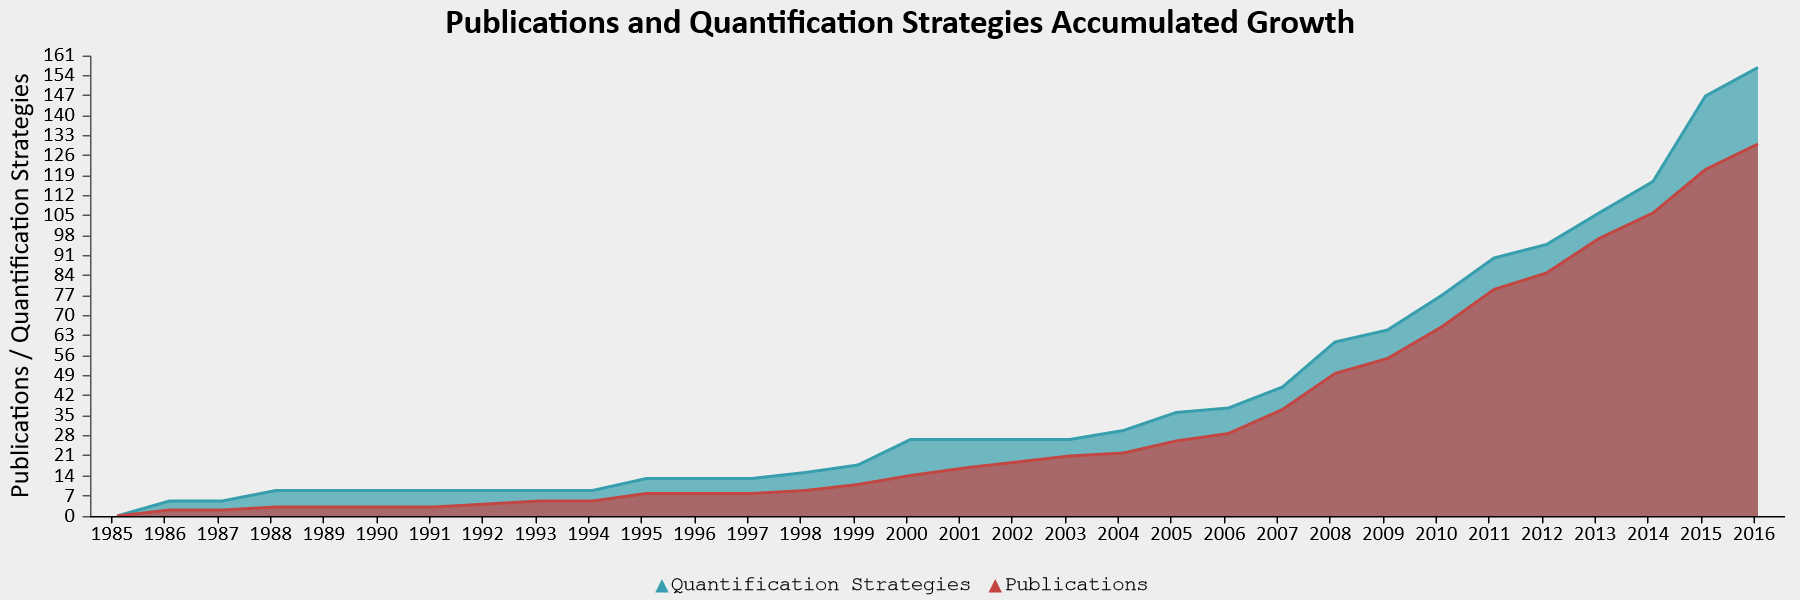
\includegraphics[width=1\linewidth]{images/flexiblemeasure} 

}

\caption{Plot of publications using CRTT (blue) and unique quantifications of the measure (red). Figure from FlexibleMeasures.com by Malte Elson}\label{fig:flexiblemeasure}
\end{figure}

\hypertarget{optionalstopping}{%
\section{Optional stopping}\label{optionalstopping}}



\begin{figure}

{\centering 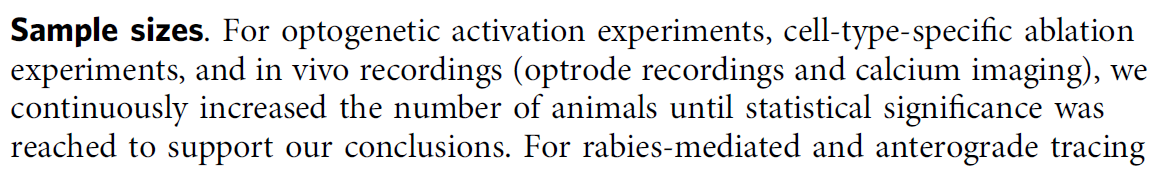
\includegraphics[width=1\linewidth]{images/optionalstoppingexample} 

}

\caption{Screenshot a scientific paper explicitly admitting to using optional stopping.}\label{fig:optionalstoppingexample}
\end{figure}

One practice that inflates the Type 1 error rate is known as \textbf{optional stopping}. In optional stopping, a researcher repeatedly analyzes the data, continues the data collection when the test result is not statistically significant, but stops when a significant effect is observed. The quote from a published article in the figure above is an example where researchers transparently report they used optional stopping, but more commonly people do not disclose the use of optional stopping in their methods sections. In recent years, many researchers have learned that optional stopping is problematic. This has lead some to the general idea that you should not collect data, look at whether the results are significant, and stop data collection when the result is significant, or if not, continue data collection. That is not the correct conclusion, and is an example of becoming too inflexible. The correct approach - to collect data in batches, called \textbf{sequential analysis} - has been extensively developed by statisticians, and is used in many medical trials. We will discuss \protect\hyperlink{sequential}{sequential analyses in a dedicated chapter}. The main lesson is that certain research practices can increase the flexibility and efficiency of studies you perform, when done right, but the same practices can inflate the Type 1 error rate when done wrong. Let's therefore try to get a better understanding when we are inflating our Type 1 error rate with optional stopping, and how to do this correctly using sequential analysis.

Copy the code below into R and run it. This script will simulate an ongoing data collection. After 10 participants in each condition, a \emph{p}-value is calculated by performing an independent \emph{t}-test, and this \emph{t}-test is then repeated after every additional participant that is collected. Then, all these \emph{p}-values are plotted as a function of the increasing sample size.

\begin{Shaded}
\begin{Highlighting}[]
\NormalTok{n }\OtherTok{\textless{}{-}} \DecValTok{200} \CommentTok{\# total number of datapoints (per condition) after initial 10}
\NormalTok{d }\OtherTok{\textless{}{-}} \FloatTok{0.0} \CommentTok{\# effect size d}

\NormalTok{p }\OtherTok{\textless{}{-}} \FunctionTok{numeric}\NormalTok{(n) }\CommentTok{\# store p{-}values}
\NormalTok{x }\OtherTok{\textless{}{-}} \FunctionTok{numeric}\NormalTok{(n) }\CommentTok{\# store x{-}values}
\NormalTok{y }\OtherTok{\textless{}{-}} \FunctionTok{numeric}\NormalTok{(n) }\CommentTok{\# store y{-}values}

\NormalTok{n }\OtherTok{\textless{}{-}}\NormalTok{ n }\SpecialCharTok{+} \DecValTok{10} \CommentTok{\# add 10 to number of datapoints}

\ControlFlowTok{for}\NormalTok{ (i }\ControlFlowTok{in} \DecValTok{10}\SpecialCharTok{:}\NormalTok{n) \{ }\CommentTok{\# for each simulated participants after the first 10}
\NormalTok{  x[i] }\OtherTok{\textless{}{-}} \FunctionTok{rnorm}\NormalTok{(}\AttributeTok{n =} \DecValTok{1}\NormalTok{, }\AttributeTok{mean =} \DecValTok{0}\NormalTok{, }\AttributeTok{sd =} \DecValTok{1}\NormalTok{)}
\NormalTok{  y[i] }\OtherTok{\textless{}{-}} \FunctionTok{rnorm}\NormalTok{(}\AttributeTok{n =} \DecValTok{1}\NormalTok{, }\AttributeTok{mean =}\NormalTok{ d, }\AttributeTok{sd =} \DecValTok{1}\NormalTok{)}
\NormalTok{  p[i] }\OtherTok{\textless{}{-}} \FunctionTok{t.test}\NormalTok{(x[}\DecValTok{1}\SpecialCharTok{:}\NormalTok{i], y[}\DecValTok{1}\SpecialCharTok{:}\NormalTok{i], }\AttributeTok{var.equal =} \ConstantTok{TRUE}\NormalTok{)}\SpecialCharTok{$}\NormalTok{p.value}
\NormalTok{\}}

\NormalTok{p }\OtherTok{\textless{}{-}}\NormalTok{ p[}\DecValTok{10}\SpecialCharTok{:}\NormalTok{n] }\CommentTok{\# Remove first 10 empty p{-}values}

\CommentTok{\# Create the plot}
\FunctionTok{par}\NormalTok{(}\AttributeTok{bg =} \StringTok{"\#fffafa"}\NormalTok{)}
\FunctionTok{plot}\NormalTok{(}\DecValTok{0}\NormalTok{, }\AttributeTok{col =} \StringTok{"red"}\NormalTok{, }\AttributeTok{lty =} \DecValTok{1}\NormalTok{, }\AttributeTok{lwd =} \DecValTok{3}\NormalTok{, }\AttributeTok{ylim =} \FunctionTok{c}\NormalTok{(}\DecValTok{0}\NormalTok{, }\DecValTok{1}\NormalTok{), }\AttributeTok{xlim =} \FunctionTok{c}\NormalTok{(}\DecValTok{10}\NormalTok{, n), }
     \AttributeTok{type =} \StringTok{"l"}\NormalTok{, }\AttributeTok{xlab =} \StringTok{"sample size"}\NormalTok{, }\AttributeTok{ylab =} \StringTok{"p{-}value"}\NormalTok{)}
\FunctionTok{lines}\NormalTok{(p, }\AttributeTok{lwd =} \DecValTok{2}\NormalTok{)}
\FunctionTok{abline}\NormalTok{(}\AttributeTok{h =} \FloatTok{0.05}\NormalTok{, }\AttributeTok{col =} \StringTok{"darkgrey"}\NormalTok{, }\AttributeTok{lty =} \DecValTok{2}\NormalTok{, }\AttributeTok{lwd =} \DecValTok{2}\NormalTok{) }\CommentTok{\# draw line at p = 0.05}

\FunctionTok{min}\NormalTok{(p) }\CommentTok{\# Return lowest p{-}value from all looks}
\FunctionTok{cat}\NormalTok{(}\StringTok{"The lowest p{-}value was observed at sample size"}\NormalTok{, }\FunctionTok{which.min}\NormalTok{(p) }\SpecialCharTok{+} \DecValTok{10}\NormalTok{) }
\FunctionTok{cat}\NormalTok{(}\StringTok{"The p{-}value dropped below 0.05 for the first time at sample size:"}\NormalTok{, }
    \FunctionTok{ifelse}\NormalTok{(}\FunctionTok{is.na}\NormalTok{(}\FunctionTok{which}\NormalTok{(p }\SpecialCharTok{\textless{}} \FloatTok{0.05}\NormalTok{)[}\DecValTok{1}\NormalTok{] }\SpecialCharTok{+} \DecValTok{10}\NormalTok{), }\StringTok{"NEVER"}\NormalTok{, }\FunctionTok{which}\NormalTok{(p }\SpecialCharTok{\textless{}} \FloatTok{0.05}\NormalTok{)[}\DecValTok{1}\NormalTok{] }\SpecialCharTok{+} \DecValTok{10}\NormalTok{)) }
\end{Highlighting}
\end{Shaded}

For example, in the Figure below, you see the \emph{p}-value plotted on the y-axis (from 0 to 1) and the sample size plotted on the x-axis (from 0 to 200). For this simulation, the true effect size was d = 0, meaning there is no true effect. We can thus only observe true negatives or false positives. As the sample size increases, the \emph{p}-value slowly moves up and down (remember from the chapter on \protect\hyperlink{pvalues}{\emph{p}-values} that when there is no true effect, \emph{p}-values are uniformly distributed). In Figure \ref{fig:animatep}, the \emph{p}-value drops below the grey line (indicating an alpha level 0.05) after collecting 83 participants in each condition, only to drift back upwards to larger \emph{p}-values. From this figure, it becomes clear that the more often we look at the data, and the larger the total sample size, the higher the probability that one of the analyses will yield a p \textless{} \(\alpha\). If resources are infinite, the Type 1 error rate will be 1, and a researcher can always find a significant result through optional stopping.



\begin{figure}

{\centering 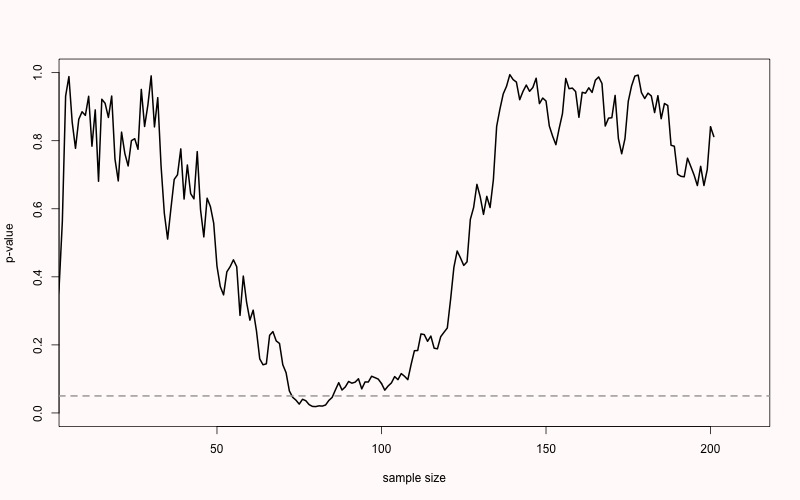
\includegraphics[width=1\linewidth]{images/animatep} 

}

\caption{Simulated \emph{p}-values for each additional observation when the null is true.}\label{fig:animatep}
\end{figure}

When there \emph{is} a true effect, we see that \emph{p}-values also vary, but they will eventually drop to below the alpha level. Due to the variation, we just do not know exactly when. When we perform an a-priori power analysis, we can compute the probability that looking at a specific sample size will yield a significant \emph{p}-value. In Figure \ref{fig:animatep2} we see the same simulation, but now when there is a true but small effect of d = 0.3. With 200 observations per condition, a sensitivity power analysis reveals that we have 85\% power. If we would analyze the data at an interim analysis (e.g., after 150 observations) we would often already find a statistically significant effect (as we would have 74\% power). This illustrates a benefit of sequential analyses, where we control error rates, but can stop early at an interim analysis. Sequential analyses are especially useful in large or expensive studies where there is uncertainty about the true effect size.



\begin{figure}

{\centering 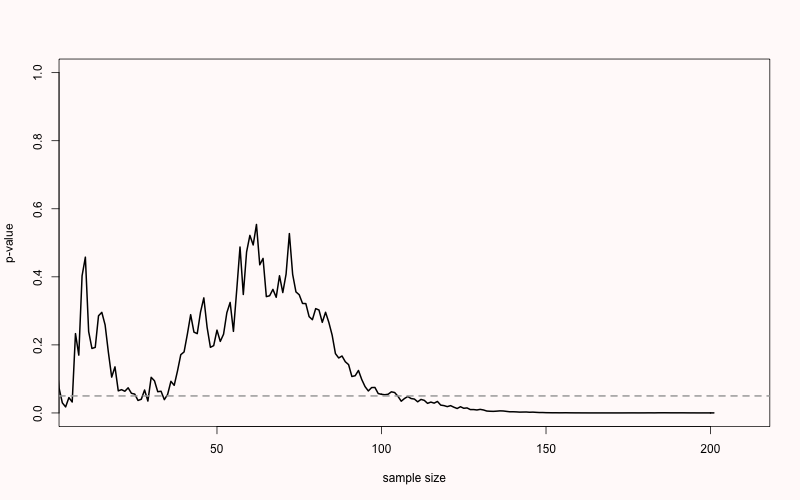
\includegraphics[width=1\linewidth]{images/animatep2} 

}

\caption{Simulated \emph{p}-values for each additional observation when d = 0.3.}\label{fig:animatep2}
\end{figure}

Let's more formally examine the inflation of the Type 1 error rate through optional stopping in a \textbf{simulation study}. Copy the code below into R and run the code. Note that the 50000 simulations (needed to get the error rates reasonably accurate) take some time to run.

\begin{Shaded}
\begin{Highlighting}[]
\NormalTok{N }\OtherTok{\textless{}{-}} \DecValTok{100} \CommentTok{\# total datapoints (per condition)}
\NormalTok{looks }\OtherTok{\textless{}{-}} \DecValTok{5} \CommentTok{\# set number of looks at the data}
\NormalTok{nsims }\OtherTok{\textless{}{-}} \DecValTok{50000} \CommentTok{\# number of simulated studies}
\NormalTok{alphalevel }\OtherTok{\textless{}{-}} \FloatTok{0.05} \CommentTok{\# set alphalevel}

\ControlFlowTok{if}\NormalTok{(looks }\SpecialCharTok{\textgreater{}} \DecValTok{1}\NormalTok{)\{}
\NormalTok{  look\_at\_n }\OtherTok{\textless{}{-}} \FunctionTok{ceiling}\NormalTok{(}\FunctionTok{seq}\NormalTok{(N }\SpecialCharTok{/}\NormalTok{ looks, N, (N }\SpecialCharTok{{-}}\NormalTok{ (N }\SpecialCharTok{/}\NormalTok{ looks)) }\SpecialCharTok{/}\NormalTok{ (looks }\SpecialCharTok{{-}} \DecValTok{1}\NormalTok{)))}
\NormalTok{\}  }\ControlFlowTok{else}\NormalTok{ \{}
\NormalTok{  look\_at\_n }\OtherTok{\textless{}{-}}\NormalTok{ N}
\NormalTok{\}}
\NormalTok{look\_at\_n }\OtherTok{\textless{}{-}}\NormalTok{ look\_at\_n[look\_at\_n }\SpecialCharTok{\textgreater{}} \DecValTok{2}\NormalTok{] }\CommentTok{\# Remove looks at N of 1 or 2}
\NormalTok{looks}\OtherTok{\textless{}{-}}\FunctionTok{length}\NormalTok{(look\_at\_n) }\CommentTok{\# if looks are removed, update number of looks}

\NormalTok{matp }\OtherTok{\textless{}{-}} \FunctionTok{matrix}\NormalTok{(}\ConstantTok{NA}\NormalTok{, }\AttributeTok{nrow =}\NormalTok{ nsims, }\AttributeTok{ncol =}\NormalTok{ looks) }\CommentTok{\# Matrix for p{-}values l tests}
\NormalTok{p }\OtherTok{\textless{}{-}} \FunctionTok{numeric}\NormalTok{(nsims) }\CommentTok{\# Variable to save pvalues}

\CommentTok{\# Loop data generation for each study, then loop to perform a test for each N}
\ControlFlowTok{for}\NormalTok{ (i }\ControlFlowTok{in} \DecValTok{1}\SpecialCharTok{:}\NormalTok{nsims) \{}
\NormalTok{  x }\OtherTok{\textless{}{-}} \FunctionTok{rnorm}\NormalTok{(}\AttributeTok{n =}\NormalTok{ N, }\AttributeTok{mean =} \DecValTok{0}\NormalTok{, }\AttributeTok{sd =} \DecValTok{1}\NormalTok{)}
\NormalTok{  y }\OtherTok{\textless{}{-}} \FunctionTok{rnorm}\NormalTok{(}\AttributeTok{n =}\NormalTok{ N, }\AttributeTok{mean =} \DecValTok{0}\NormalTok{, }\AttributeTok{sd =} \DecValTok{1}\NormalTok{)}
  \ControlFlowTok{for}\NormalTok{ (j }\ControlFlowTok{in} \DecValTok{1}\SpecialCharTok{:}\NormalTok{looks) \{}
\NormalTok{    matp[i, j] }\OtherTok{\textless{}{-}} \FunctionTok{t.test}\NormalTok{(x[}\DecValTok{1}\SpecialCharTok{:}\NormalTok{look\_at\_n[j]], y[}\DecValTok{1}\SpecialCharTok{:}\NormalTok{look\_at\_n[j]], }
                         \AttributeTok{var.equal =} \ConstantTok{TRUE}\NormalTok{)}\SpecialCharTok{$}\NormalTok{p.value }\CommentTok{\# perform the t{-}test, store}
\NormalTok{  \}}
  \FunctionTok{cat}\NormalTok{(}\StringTok{"Loop"}\NormalTok{, i, }\StringTok{"of"}\NormalTok{, nsims, }\StringTok{"}\SpecialCharTok{\textbackslash{}n}\StringTok{"}\NormalTok{)}
\NormalTok{\}}

\CommentTok{\# Save Type 1 error rate smallest p at all looks}
\ControlFlowTok{for}\NormalTok{ (i }\ControlFlowTok{in} \DecValTok{1}\SpecialCharTok{:}\NormalTok{nsims) \{}
\NormalTok{  p[i] }\OtherTok{\textless{}{-}} \FunctionTok{ifelse}\NormalTok{(}\FunctionTok{length}\NormalTok{(matp[i,}\FunctionTok{which}\NormalTok{(matp[i,] }\SpecialCharTok{\textless{}}\NormalTok{ alphalevel)]) }\SpecialCharTok{==} \DecValTok{0}\NormalTok{, }
\NormalTok{                 matp[i,looks], matp[i,}\FunctionTok{which}\NormalTok{(matp[i,] }\SpecialCharTok{\textless{}}\NormalTok{ alphalevel)])}
\NormalTok{\}}

\FunctionTok{hist}\NormalTok{(p, }\AttributeTok{breaks =} \DecValTok{100}\NormalTok{, }\AttributeTok{col =} \StringTok{"grey"}\NormalTok{) }\CommentTok{\# create plot}
\FunctionTok{abline}\NormalTok{(}\AttributeTok{h =}\NormalTok{ nsims }\SpecialCharTok{/} \DecValTok{100}\NormalTok{, }\AttributeTok{col =} \StringTok{"red"}\NormalTok{, }\AttributeTok{lty =} \DecValTok{3}\NormalTok{)}

\FunctionTok{cat}\NormalTok{(}\StringTok{"Type 1 error rates for look 1 to"}\NormalTok{, looks, }\StringTok{":"}\NormalTok{, }
    \FunctionTok{colSums}\NormalTok{(matp }\SpecialCharTok{\textless{}}\NormalTok{ alphalevel) }\SpecialCharTok{/}\NormalTok{ nsims)}
\FunctionTok{cat}\NormalTok{(}\StringTok{"Type 1 error rate when only the lowest p{-}value for all looks is reported:"}\NormalTok{, }
    \FunctionTok{sum}\NormalTok{(p }\SpecialCharTok{\textless{}}\NormalTok{ alphalevel) }\SpecialCharTok{/}\NormalTok{ nsims)}
\end{Highlighting}
\end{Shaded}

This simulation will perform multiple independent \emph{t}-tests on simulated data, looking multiple times until the maximum sample size is reached. In the first four lines, you can set the most important parameters of the simulation. First, the maximum sample size in each condition (e.g., 100). Then, the number of looks (e.g., 5). At best, you can look at the data after every participant (e.g., with 100 participants, you can look 100 times -- or actually 98 times, because you need more than 2 participants in each condition for a \emph{t}-test!). You can set the number of simulations (the more, the clearer the pattern will be, but the longer the simulation takes), and the alpha level (e.g., 0.05). Since you can only make a Type 1 error when there is no true effect, the effect size is set to 0 in these simulations.

When you perform only a single test, the Type 1 error rate is the probability of finding a \emph{p}-value lower than your alpha level, when there is no effect. In an optional stopping scenario where you look at the data twice, the Type 1 error rate is the probability of finding a \emph{p}-value lower than your alpha level at the first look, \textbf{and} the probability of \textbf{not} finding a \emph{p}-value lower than your alpha level at the \textbf{first} look, but finding a \emph{p}-value lower than your alpha level at the \textbf{second} look. This is a \emph{conditional probability}, which makes error control a little bit more complex than when multiple looks are completely independent.

So how much does optional stopping inflate the Type 1 error rate? And which \emph{p}-values can we expect under optional stopping?

Start by running the simulation without changing any values, so simulating 100 participants in each condition, looking 5 times at your data, with an alpha of 0.05. Note the 50.000 simulations take a while! You should see something similar to Figure \ref{fig:optionalstopfig} below (which is based on 500.000 simulations to make the pattern very clear).



\begin{figure}

{\centering 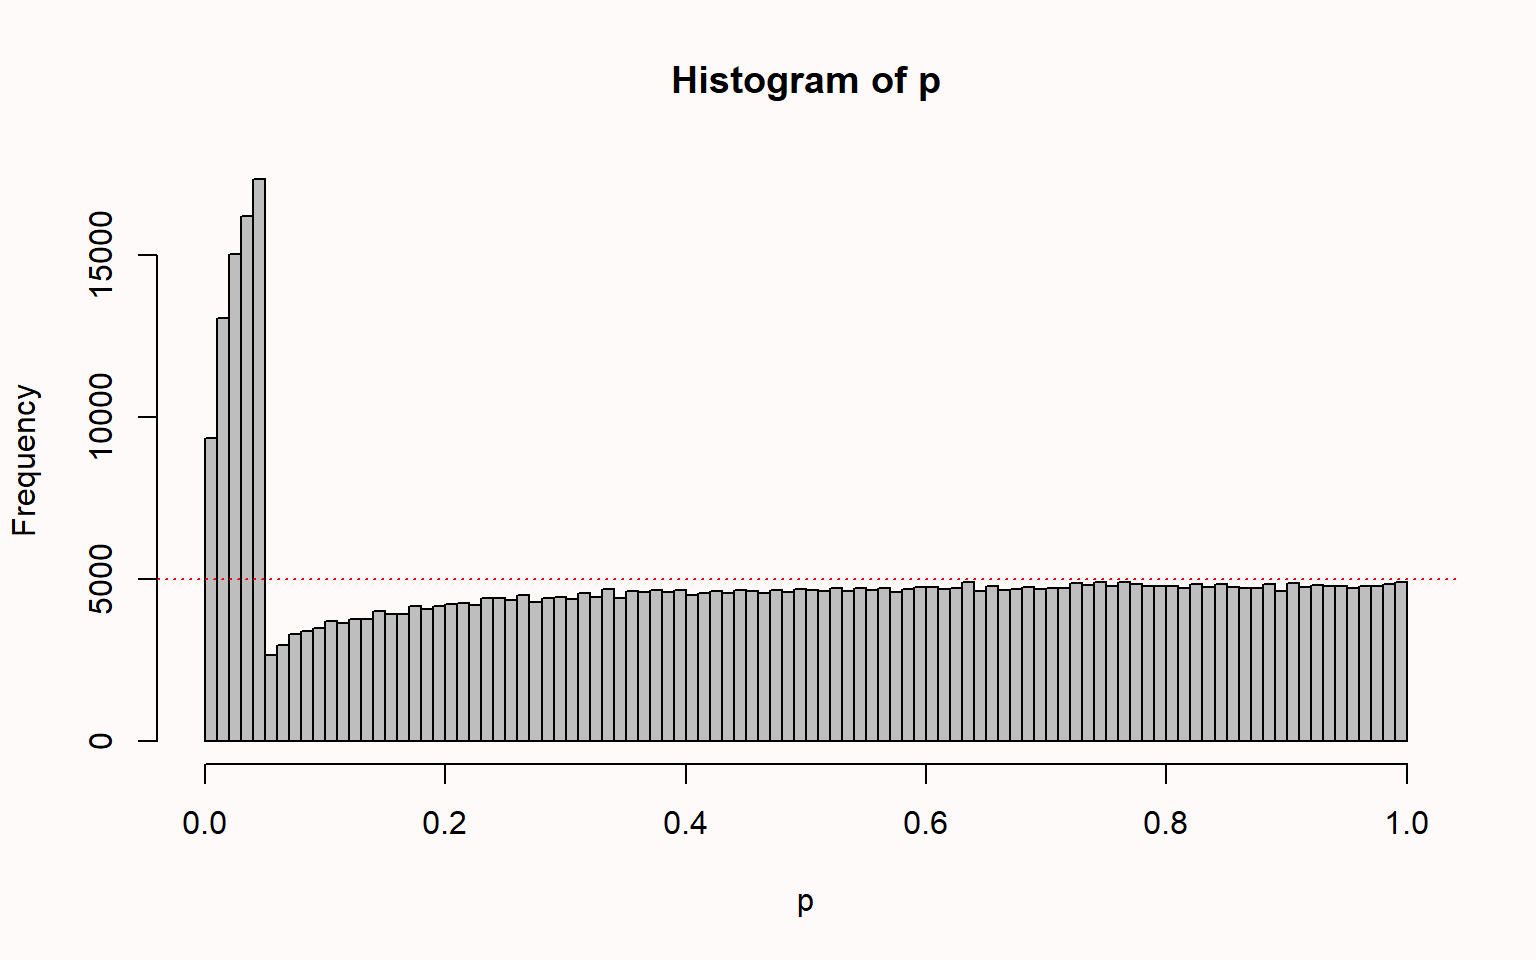
\includegraphics[width=1\linewidth]{02-errorcontrol_files/figure-latex/optionalstopfig-1} 

}

\caption{Simulation of 500000 studies performing 5 interim analyses at an alpha level of 5\%.}\label{fig:optionalstopfig}
\end{figure}

We see 100 bars, one for each \% (so one for all \emph{p}-values between 0.00 and 0.01, one for \emph{p}-values between 0.01 and 0.02, etc.). There is a horizontal line that indicates where all \emph{p}-values should fall, if they would be uniformly distributed (as they should be when there is no true effect, as explained in the chapter on \protect\hyperlink{pvalues}{\emph{p}-values}).

The distribution of \emph{p}-values is peculiar. We see that compared to a uniform distributions, a bunch of results just above the alpha threshold of 0.05 are missing, and they seem to have been pulled just below 0.05, where there is a much higher frequency of outcomes compared to when data is not analyzed multiple times as it comes in. Notice how relatively high \emph{p}-values (e.g., \emph{p} = 0.04) are more common than lower \emph{p}-values (e.g., 0.01). We will see in the chapter on \href{bias}{bias detection} that statistical techniques such as \emph{p}-curve analysis can pick up on this pattern.

When using an alpha level of 5\% with 5 looks at the data, the overall Type 1 error rate has inflated to 14\%. If we lower the alpha level at each interim analysis, the overall Type 1 error rate can be controlled. The shape of the \emph{p}-value distribution will still look peculiar, but the total number of significant test results will be controlled at the desired alpha level. The well-known Bonferroni correction (i.e., using an alpha level of \(\alpha\) / the number of looks), but the \href{https://en.wikipedia.org/wiki/Pocock_boundary}{Pocock correction} is slightly more efficient. For more information on how to perform interim analyses while controlling error rates, see the dedicated chapter on \protect\hyperlink{sequential}{sequential analysis}.

\hypertarget{justifyerrorrate}{%
\section{Justifying Error Rates}\label{justifyerrorrate}}

\begin{quote}
If we reject \(H_0\) , we may reject it when it is true; if we accept \(H_0\) , we may be accepting it when it is false, that is to say, when really some alternative Bt is true. These two sources of error can rarely be eliminated completely; in some cases it will be more important to avoid the first, in others the second. We are reminded of the old problem considered by Laplace of the number of votes in a court of judges that should be needed to convict a prisoner. Is it more serious to convict an innocent man or to acquit a guilty? That will depend upon the consequences of the error; whether the punishment is death or a fine; what the danger is to the community of released criminals; and what are the current ethical views on punishment. From the point of view of mathematical theory, all that we can do is to show how the risk of the errors may be controlled and minimised. The use of these statistical tools in any given case, in determining just how the balance should be struck, must be left to the investigator.
\end{quote}

Even though in \emph{theory} the Type 1 and Type 2 error rate should be justified by the researcher (as Neyman and Pearson \citeyearpar{neyman_problem_1933} write above), in \emph{practice} researchers tend to imitate others. The default use of an alpha level of 0.05 can already be found in the work of Gosset on the \emph{t}-distribution \citep{cowles_origins_1982, kennedy-shaffer_before_2019}, who believed that a difference of two standard deviations (a z-score of 2) was sufficiently rare. The default use of 80\% power (or a 20\% Type 2 error rate) is similarly based on personal preferences by \citet{cohen_statistical_1988}, who writes:

\begin{quote}
It is proposed here as a convention that, when the investigator has no other basis for setting the desired power value, the value .80 be used. This means that beta is set at .20. This value is offered for several reasons (Cohen, 1965, pp.~98-99). The chief among them takes into consideration the implicit convention for alpha of .05. The beta of .20 is chosen with the idea that the general relative seriousness of these two kinds of errors is of the order of .20/.05, i.e., that Type I errors are of the order of four times as serious as Type II errors. This .80 desired power convention is offered with the hope that it will be ignored whenever an investigator can find a basis in his substantive concerns about his specific research investigation to choose a value ad hoc.
\end{quote}

We see that conventions are built on conventions: the norm to aim for 80\% power is built on the norm to set the alpha level at 5\%. Although there is nothing special about an alpha level of 5\%, it is interesting to reflect on why it has become so widely established. Irwin Bross \citeyearpar{bross_critical_1971} argues the use of an alpha level is functional and efficient when seen as an aspect of communication networks among scientists, and writes ``Thus the specification of the critical levels {[}\ldots{]} has proved in practice to be an effective method for controlling the noise in communication networks.''
Bross believes the 0.05 threshold is \emph{somewhat}, but not \emph{completely} arbitrary, and asks us to imagine what would have happened had an alpha level of 0.001 been proposed, or an alpha level of 0.20. In both cases, he believes the convention would not have spread -- in the first case because in many fields there are not sufficient resources to make claims at such a low error rate, and in the second case because few researchers would have found that alpha level a satisfactory quantification of `rare' events.
\citet{uygun_tunc_epistemic_2021} argue that one possible reason is that, as far as conventions go, an alpha level of 5\% might be low enough such that peers take any claims made with this error rate seriously, while at the same time being high enough such that peers will be motivated to perform an independent replication study to increase or decrease our confidence in the claim. Although lower error rates would establish claims more convincingly, this would also require more resources. One might speculate that in research areas where not every claim is important enough to a careful justification of costs and benefits, 5\% has a pragmatic function in facilitating conjectures and refutations in fields that otherwise lack a coordinated approach to knowledge generation, but are faced with limited resources.

Nevertheless, some researchers have proposed to move away from the default use of a 5\% alpha level. For example, \citet{johnson_revised_2013} proposes a default significance level of 0.005 or 0.001. Others have cautioned against such blanket recommendation because the additional resources required to reduce the Type 1 error rate might not be worth the costs \citep{lakens_justify_2018}. A lower alpha lever requires a larger sample size to achieve the same statistical power. If the sample size cannot be increased, a lower alpha level reduces the statistical power, and increases the Type 2 error rate. Whether that is desirable should be evaluated on a case by case basis.

There are two main reasons to abandon the universal use of a 5\% alpha level. The first reason to carefully choose an alpha level is that decision-making becomes more efficient \citep{mudge_setting_2012}. If researchers use hypothesis tests to make dichotomous decisions from a methodological falsificationist approach to statistical inferences, and have a certain maximum sample size they are willing or able to collect, it is typically possible to make decisions more efficiently by choosing error rates such that the combined cost of Type 1 and Type 2 errors is minimized. If we aim to either minimize or balance Type 1 and Type 2 error rates for a given sample size and effect size, the alpha level should be set not based on convention, but by weighting the relative cost of both types of errors \citep{maier_justify_2022}.

For example, imagine a researcher plans to collect 64 participants per condition to detect a d = 0.5 effect, and weighs the cost of Type 1 errors 4 times as much as Type 2 errors. This is exactly the scenario Cohen (1988) described, and with 64 participants per condition the relative weight of Type 1 and Type 2 errors yields a 5\% Type 1 error rate and a 20\% Type 2 error rate. Now imagine this researcher realizes they have the resources to collect 80 observations instead of just 64. With an interest in an effect size of d = 0.5, the relative weight of Type 1 and Type 2 errors of 4 would be satisfied when they set the alpha level to 0.037 as then the Type 2 error rate is 0.147. Alternatively, the researcher might have decided to collect 64 observations, but not balance the error rates, but set the alpha level such that the weighted combined error rate is minimized, which is achieved when the alpha level is set to 0.033, as visualized in Figure \ref{fig:minimizeerror} (for further information, see \citet{maier_justify_2022}).

\begin{figure}

{\centering 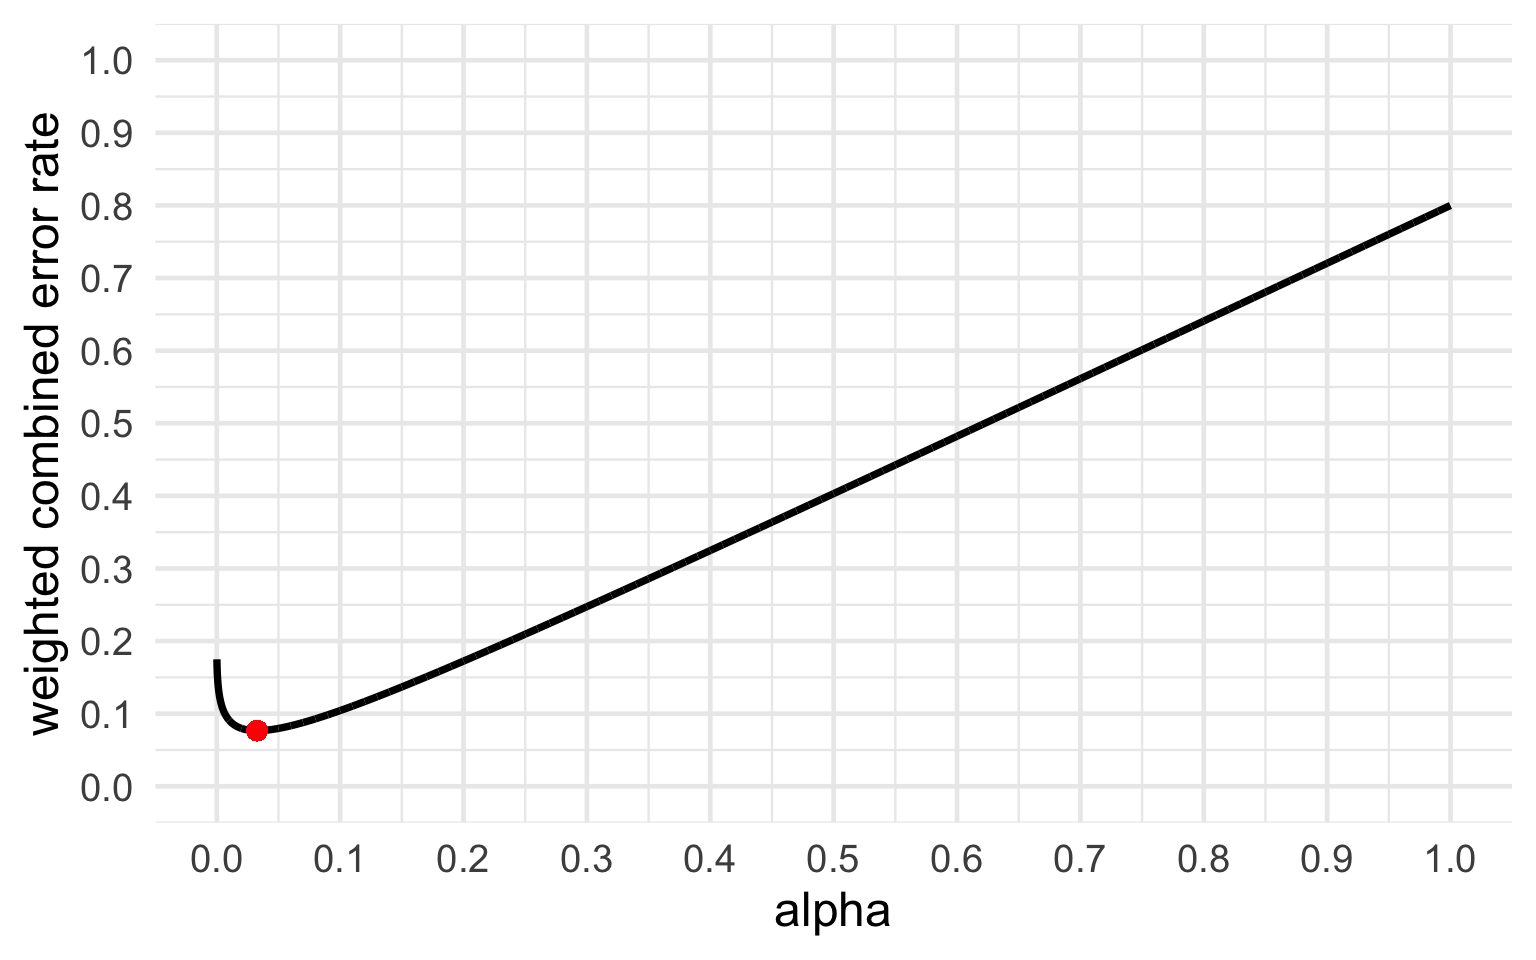
\includegraphics[width=1\linewidth]{02-errorcontrol_files/figure-latex/minimizeerror-1} 

}

\caption{Weighted combined error rate, minimized at alpha = 0.037.}\label{fig:minimizeerror}
\end{figure}

Justifying error rates can lead to situations where the alpha level is increased above 0.05, because this leads to more optimal decision making. Winer (1962) writes:

\begin{quote}
The frequent use of the .05 and .01 levels of significance is a matter of convention having little scientific or logical basis. When the power of tests is likely to be low under these levels of significance, and when Type 1 and Type 2 errors are of approximately equal importance, the .30 and .20 levels of significance may be more appropriate than the .05 and .01 levels.''
\end{quote}

The reasoning here is that a design that has 70\% power for the smallest effect size of interest would not balance the Type 1 and Type 2 error rates in a sensible manner. Of course, such an increase of the alpha level should only be deemed acceptable when authors can justify that the costs of the increase in the Type 1 error rate is sufficiently compensated by the benefit of decreased Type 2 error rate. This will encompass cases where (1) the study will have practical implications that require decision making, (2) a cost-benefit analysis is provided that gives a clear rationale for relatively high costs of a Type 2 error, (3) the probability that \(H_1\) is false is relatively low, and (4) it is not feasible to reduce overall error rates by collecting more data.

One should also carefully reflect on the choice of the alpha level when an experiment achieves very high statistical power for all effect sizes that are considered meaningful. If a study has 99\% power for effect sizes of interest, and thus a 1\% Type 2 error rate, but uses the default 5\% alpha level, it also suffers from a lack of balance, and the use of a lower alpha level would lead to a more balanced decision, and increase the severity of the test.

The second reason is most relevant for large data sets, and is related to \protect\hyperlink{lindley}{Lindley's paradox}. As the statistical power increases, some \emph{p}-values below 0.05 (e.g., \emph{p} = 0.04) can be more likely when there is \emph{no} effect than when there \emph{is} an effect. To prevent situations where a frequentist rejects the null hypothesis based on \emph{p} \textless{} 0.05, when the evidence in the test favors the null hypothesis over the alternative hypothesis, it is recommended to lower the alpha level as a function of the sample size. The need to do so is discussed by \citet{leamer_specification_1978}, who writes ``The rule of thumb quite popular now, that is, setting the significance level arbitrarily to .05, is shown to be deficient in the sense that from every reasonable viewpoint the significance level should be a decreasing function of sample size.'' The idea of this approach is to reduce the alpha level such that a Bayes factor or likelihood computed for a significant result would never be evidence \emph{for} the null hypothesis (for an online Shiny app to perform such calculations, see \href{https://shiny.ieis.tue.nl/JustifyAlpha/}{here}.

\begin{verbatim}
## NULL
\end{verbatim}

\hypertarget{why-you-dont-need-to-adjust-your-alpha-level-for-all-tests-youll-do-in-your-lifetime.}{%
\section{Why you don't need to adjust your alpha level for all tests you'll do in your lifetime.}\label{why-you-dont-need-to-adjust-your-alpha-level-for-all-tests-youll-do-in-your-lifetime.}}

Some researchers criticize corrections for multiple comparisons because one might as well correct for all tests you do in your lifetime \citep{perneger_whats_1998}. If you choose to use a Neyman-Pearson approach to statistics the only reason to correct for all tests you perform in your lifetime is when all the work you have done in your life tests a single theory, and you would use your last words to decide to accept or reject this theory, as long as only one of all individual tests you have performed yielded a \emph{p} \textless{} \(\alpha\). Researchers rarely work like this.

Instead, in a Neyman-Pearson approach to hypothesis testing, the goal is to use data to make decisions about how to act. Neyman \citeyearpar{neyman_inductive_1957} calls his approach \textbf{inductive behavior}. The outcome of an experiment leads one to take different possible actions, which can be either practical (e.g., implement a new procedure, abandon a research line) or scientific (e.g., claim there is or is no effect). From an error-statistical approach \citep{mayo_statistical_2018} inflated Type 1 error rates mean that it has become very likely that you will be able to claim support for your hypothesis, even when the hypothesis is wrong. This reduces the severity of the test. To prevent this, we need to control our error rate at the level of our claim.

A useful distinction in the literature on multiple testing is a \textbf{union-intersection} testing approach, and an \textbf{intersection-union} testing approach \citep{dmitrienko_traditional_2013}. In a union-intersection approach, a claim is made when \emph{at-least-one} test is significant. In these cases, a correction for multiple comparisons is required to control the error rate. In an intersection-union approach, a claim is made when all performed tests are statistically significant, and no correction for multiple comparisons is required (and indeed, under some assumptions researchers could even \emph{increase} the alpha level in a intersection-union approach).

Let's assume we collect data from 100 participants in a control and treatment condition. We collect 3 dependent variables (dv1, dv2, and dv3). In the population there is no difference between groups on any of these three variables (the true effect size is 0). We will analyze the three dv's in independent \emph{t}-tests. This requires specifying our alpha level, and thus deciding whether we need to correct for multiple comparisons. For some reason I do not fully understand, several researchers believe it is difficult to decide when you need to correct for multiple comparisons. As Bretz, Hothorn, \& Westfall \citeyearpar{bretz_multiple_2011} write in their excellent book ``Multiple Comparisons Using R'': ``The appropriate choice of null hypotheses being of primary interest is a controversial question. That is, it is not always clear which set of hypotheses should constitute the family H1,\ldots,Hm. This topic has often been in dispute and there is no general consensus.'' In one of the best papers on controlling for multiple comparisons out there, \citet{bender_adjusting_2001} write: ``Unfortunately, there is no simple and unique answer to when it is appropriate to control which error rate. Different persons may have different but nevertheless reasonable opinions. In addition to the problem of deciding which error rate should be under control, it has to be defined first which tests of a study belong to one experiment.''

I have never understood this confusion, at least not when working within a Neyman-Pearson approach to hypothesis testing, where the goal is to control error rates at the level of a \emph{statistical claim}. How we control error rates depends on the claim(s) we want to make. We might want to act as if (or claim that) our treatment works if there is a difference between the treatment and control conditions on any of the three variables. This means we consider the prediction corroborated when the \emph{p}-value of the first \emph{t}-test is smaller than alpha level, the \emph{p}-value of the second \emph{t}-test is smaller than the alpha level, or the \emph{p}-value of the third \emph{t}-test is smaller than the alpha level. This falls under the union-intersection approach, and a researcher should correct the alpha level for multiple comparisons.

We could also want to make three different predictions. Instead of one hypothesis (``something will happen'') we have three different hypotheses, and predict there will be an effect on dv1, dv2, and dv3. Each of these claims can be corroborated, or not. As these are three tests, that inform three claims, there are no multiple comparisons, and no correction for the alpha level is required.

It might seem if researchers can get out of corrections for multiple comparisons by formulating a hypothesis for every possible test they will perform. Indeed, they can. For a ten by ten correlation matrix, a researcher might state they are testing 45 unique predictions, each at an uncorrected alpha level. However, readers might reasonably question whether these 45 tests were all predicted by a sensible theory, or if the author is just making up predictions in order to not have to correct the alpha level. Distinguishing between these two scenarios is not a \emph{statistical} question, but a \emph{theoretical} question. If only a few of the 45 tests corroborate the prediction, the meager track record of the predictions should make readers doubt the body of work that was used to derive the predictions has anything going for it.

There are different ways to control for error rates, the easiest being the Bonferroni correction an the ever-so-slightly less conservative Holm-Bonferroni sequential procedure. When the number of statistical tests becomes substantial, it is sometimes preferable to control false discovery rates, instead of error rates \citep{benjamini_controlling_1995}.

\hypertarget{power-analysis}{%
\section{Power Analysis}\label{power-analysis}}

So far we have largely focused on Type 1 error control. As was clear from Figure \ref{fig:animatep2}, when there is a true effect \emph{p}-values will eventually become smaller than an alpha level as the sample size becomes large enough. When designing an experiment, the goal is to choose a sample size that provides a desired Type 2 error rate for an effect size of interest. This can be achieved by performing an a-priori power analysis. It is important to highlight that the goal of an a-priori power analysis is \emph{not} to achieve sufficient power for the true effect size. The true effect size is always unknown when designing a study. The goal of an a-priori power analysis is to achieve sufficient power, given a specific \emph{assumption} of the effect size a researcher wants to detect. Just like a Type I error rate is the maximum probability of making a Type I error conditional on the assumption that the null hypothesis is true, an a-priori power analysis is computed under the assumption of a specific effect size. It is unknown if this assumption is correct. All a researcher can do is to make sure their assumptions are well justified. Statistical inferences based on a test where the Type II error is controlled are conditional on the assumption of a specific effect size. They allow the inference that, assuming the true effect size is at least as large as that used in the a-priori power analysis, the maximum Type II error rate in a study is not larger than a desired value.

In Figure \ref{fig:powerd} we see the expected distribution of observed standardized effect sizes (Cohen's \emph{d}) for an independent \emph{t}-test with 50 observations in each condition. The bell-shaped curve on the left represents the expectations if the null is true, and the red areas in the tail represent Type 1 errors. The bell-shaped curve on the right represents the expectations if the alternative hypothesis is true, and d = 0.5. The vertical line at d = 0.4 represents the \textbf{critical effect size}. With this sample size and an alpha level of 0.05, observed effect sizes smaller than d = 0.4 will not be statistically significant. If there is a true effect, these outcomes will be Type 2 errors, illustrated by the blue shaded area. The remainder of the curve reflects true positives, when there is a true effect, and the observed effect sizes are statistically significant. The power of the test is the percentages of the distribution on the right that is larger than the critical value.



\begin{figure}

{\centering 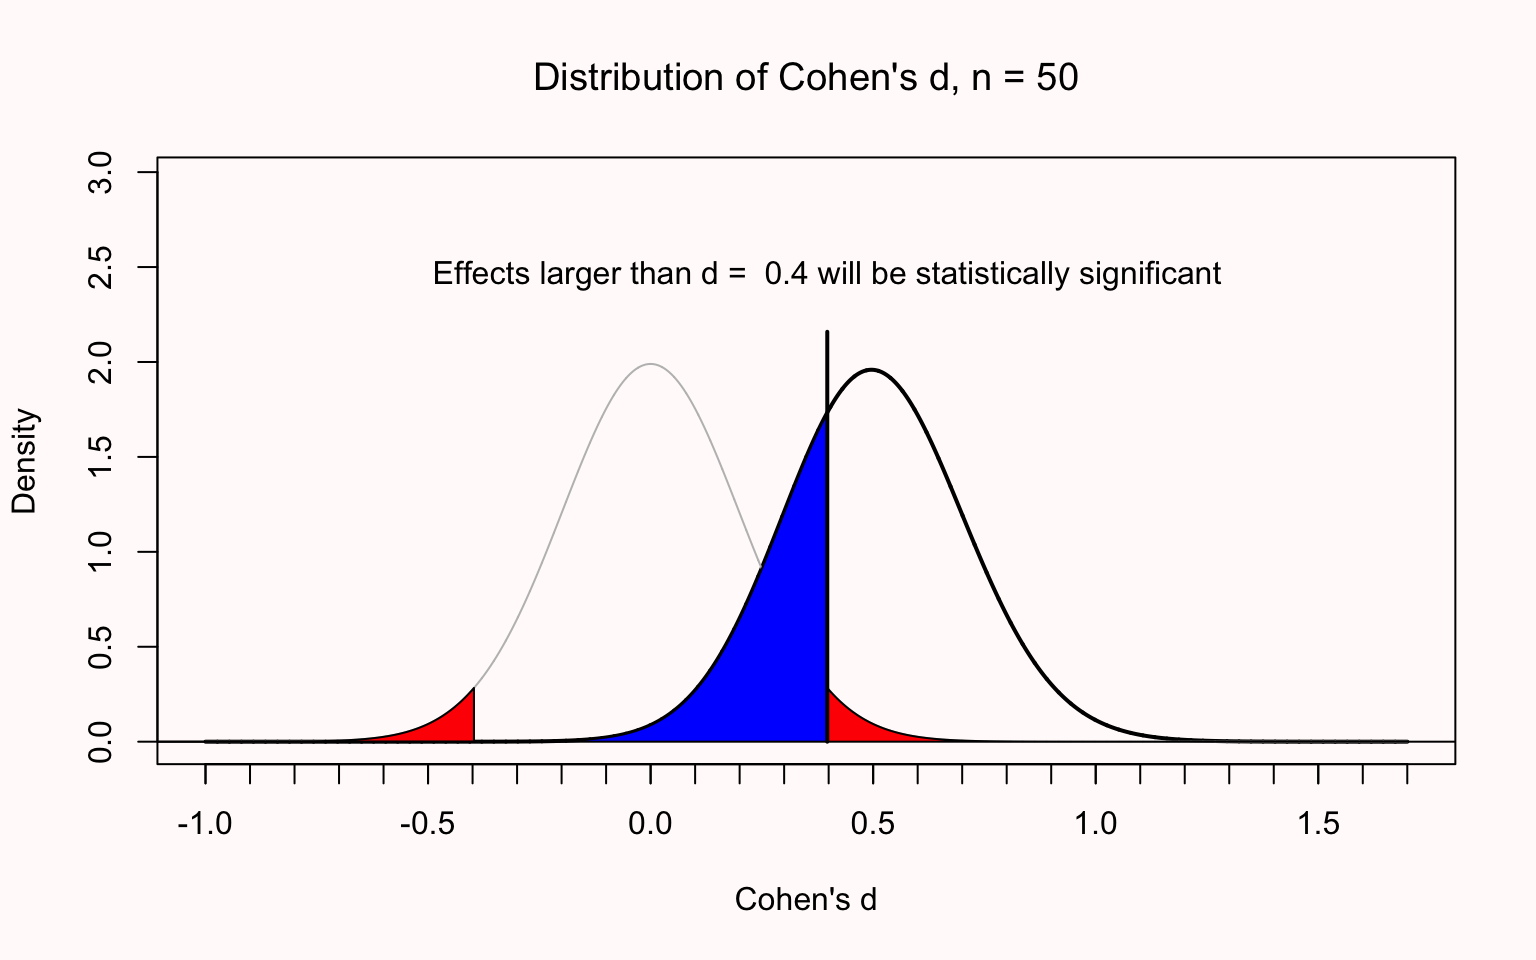
\includegraphics[width=1\linewidth]{02-errorcontrol_files/figure-latex/powerd-1} 

}

\caption{Distribution of \emph{d} = 0 and \emph{d} = 0.5 for an independent \emph{t}-test with \emph{n} = 50.}\label{fig:powerd}
\end{figure}

The issue of Type 2 error control will be discussed in more detail in the chapter on \protect\hyperlink{aprioripower}{sample size justification}. Even though the topic of Type 2 error control is only briefly discussed here, it is at least as important as Type 1 error control. An informative study should have a high probability of observing an effect if there is an effect. Indeed, the default recommendation to aim for 80\% power leaves a surprisingly large (20\%) probability of a Type 2 error. If a researcher only cares about not making a decision error, but the researcher does not care about whether this decision error is a false positive or a false negative, an argument could be made that Type 1 and Type 2 errors are weighed equally. Therefore, desiging a study with balanced error rates (e.g., a 5\% Type 1 error and 95\% power) would make sense.

\hypertarget{test-yourself-1}{%
\section{Test Yourself}\label{test-yourself-1}}

\hypertarget{questions-about-the-positive-predictive-value}{%
\subsection{Questions about the positive predictive value}\label{questions-about-the-positive-predictive-value}}

\textbf{Q1}: In the example at the start of this chapter, we see that we control the Type 1 error rate at 5\% by using an alpha of 0.05. Still, when there is a 50\% probability that \(H_0\) is true, the proportion of false positives for all experiments performed turns out to be much lower, namely 2.5\%, or 0.025. Why?

\begin{enumerate}
\def\labelenumi{\Alph{enumi})}
\tightlist
\item
  The proportion of false positives for all experiments we have performed is a variable with a distribution around the true error rate -- sometimes it's higher, sometimes it's lower, due to random variation.
\item
  The proportion of false positives for all experiments we have performed is only 5\% when \(H_0\) is true for all 200 studies.
\item
  The proportion of false positives for all experiments we have performed is only 5\% when you have 50\% power -- if power increases above 50\%, the proportion of false positives for all experiments we have performed becomes smaller.
\item
  The proportion of false positives for all experiments we have performed is only 5\% when you have 100\% power, and it becomes smaller if power is lower than 100\%.
\end{enumerate}

\textbf{Q2}: What will make the biggest difference in improving the probability that you will find a true positive? Check your answer by shifting the sliders in the online PPV app at \url{http://shinyapps.org/apps/PPV/} or \url{https://shiny.ieis.tue.nl/PPV/}

\begin{enumerate}
\def\labelenumi{\Alph{enumi})}
\tightlist
\item
  Increase the \% of a-priori true hypotheses
\item
  Decrease the \% of a-priori true hypotheses
\item
  Increase the alpha level
\item
  Decrease the alpha level
\item
  Increase the power
\item
  Decrease the power
\end{enumerate}

Increasing the power requires bigger sample sizes, or studying larger effects. Increasing the \% of a-priori true hypotheses can be done by making better predictions -- for example building on reliable findings, and relying on strong theories. These are useful recommendations if you want to increase the probability of performing studies where you find a statistically significant result.

\textbf{Q3}: Set the ``\% of a priori true hypotheses'' slider to 50\%. Leave the `\(\alpha\) level' slider at 5\%. Leave the `\% of p-hacked studies' slider at 0. The title of Ioannidis' paper is `why most published research findings are false'. One reason might be that studies often have low power. At which value for power is the PPV 50\%. In other words, at which level of power is a significant result just as likely to be true, as that it is false?

\begin{enumerate}
\def\labelenumi{\Alph{enumi})}
\tightlist
\item
  80\%
\item
  50\%
\item
  20\%
\item
  5\%
\end{enumerate}

It seems low power alone is not the best explanation for why most published findings might be false, as it is unlikely that power is low enough in the scientific literature. Ioannidis (2005) discusses some scenarios under which it becomes likely that most published research findings are false. Some of these assume that `p-hacked studies', or studies that show a significant result due to bias, enter the literature. There are good reasons to believe this happens, as we discussed in this chapter. In the `presets by Ioannidis' dropdown menu, you can select some of these situations. Explore all of them, and pay close attention to the ones where the PPV is smaller than 50\%.

\textbf{Q4}: In general, when are most published findings false? Interpret `low' and `high' in the answer options below in relation to the values in the first example in this chapter of 50\% probability \(H_1\) is true, 5\% alpha, 80\% power,
and 0\% bias.

\begin{enumerate}
\def\labelenumi{\Alph{enumi})}
\tightlist
\item
  When the probability of examining a true hypothesis is low, combined with either low power or substantial bias (e.g., p-hacking).
\item
  When the probability of examining a true hypothesis is high, combined with either low power or substantial bias (e.g., p-hacking).
\item
  When the alpha level is high, combined with either low power or substantial bias (e.g., p-hacking).
\item
  When power is low and p-hacking is high (regardless of the \% of true hypotheses one examines).
\end{enumerate}

\textbf{Q5}: Set the ``\% of a priori true hypotheses'' slider to 0\%. Set the ``\% of p-hacked studies'' slider to 0\%. Set the ``\(\alpha\) level'' slider to 5\%. Play around with the power slider. Which statement is true?
\textbf{Without \emph{p}-hacking, when the alpha level is 5\%, and when 0\% of the hypotheses are true, }

\begin{enumerate}
\def\labelenumi{\Alph{enumi})}
\tightlist
\item
  the proportion of false positives for all experiments we have performed is 100\%.
\item
  the PPV depends on the power of the studies.
\item
  regardless of the power, the PPV equals the proportion of false positives for all experiments we have performed.
\item
  regardless of the power, the proportion of false positives for all experiments we have performed is 5\%, and the PPV is 0\% (all significant results are false positives).
\end{enumerate}

\hypertarget{questions-about-optional-stopping}{%
\subsection{Questions about optional stopping}\label{questions-about-optional-stopping}}

\textbf{Q1}: Run the script that plots the \emph{p}-value as the sample size increases 20 times, and count how often the lowest \emph{p}-value ends up below 0.05 (we will calculate the long run probability of this happening through more extensive simulations later). Remember that you can click the `clipboard' icon on the top right of the code section to copy all the code to your clipboard, and paste it in RStudio.

\textbf{Q2}: If there is a true effect, we can only observe a true positive or a false negative. Change the effect size from d \textless- 0.0 to d \textless- 0.3. This is a relatively small true effect, and with 200 participants in each condition, we have 85\% power (or an 85\% probability of finding a significant effect). Run the script again. Below is one possible example of the trajectory of \emph{p}-values as the sample size increases. Run the script 20 times. Take a good look at the variation in the \emph{p}-value trajectory. Remember that at N = 200, 85\% of the times the \emph{p}-value should have ended up below 0.05. The script returns the sample size the \emph{p}-value is the lowest (which is often, but not always, at the maximum sample size, when there is a true effect) and the sample size at which the \emph{p}-value drops below 0.05 for the first time. Which statement is true?

\begin{enumerate}
\def\labelenumi{\Alph{enumi})}
\tightlist
\item
  If the \emph{p}-value drops below 0.05, it stays below 0.05.
\item
  The \emph{p}-value randomly moves between 0 and 1, and will every now and then end up below 0.05.
\item
  The \emph{p}-value often drops below 0.05 well before 200 participants in each
  condition. In around 50\% of the simulations, this already happens at N = 100.
\item
  The \emph{p}-value will typically move below 0.05 and stay there for some time,
  but given a large enough sample, it will always move back up to \emph{p} \textgreater{} 0.05.
\end{enumerate}

\textbf{Q3}: Change the effect size d \textless- 0.8, which can be regarded as a large effect. Run the script 20 times. Take a good look at the variation in the \emph{p}-value trajectory. Which statement is true?

\begin{enumerate}
\def\labelenumi{\Alph{enumi})}
\tightlist
\item
  The \emph{p}-value randomly moves between 0 and 1, and will every now and then end up below 0.05.
\item
  The \emph{p}-values drop below and stay below 0.05 much earlier than when the true effect size is 0.3.
\item
  \emph{p}-values are meaningful when effect sizes are large (e.g., d = 0.8), but meaningless when effect sizes are small (e.g., d = 0.3).
\item
  When you examine a large effect, whenever a \emph{p}-value drops below 0.05, it will always stay below 0.05 as the sample size increases.
\end{enumerate}

\textbf{Q4}: Looking at Figure \ref{fig:optionalstopfig}, which statement is true?

\begin{enumerate}
\def\labelenumi{\Alph{enumi})}
\tightlist
\item
  Optional stopping does not impact the Type 1 error rate.
\item
  Optional stopping inflates the Type 1 error rate. We can see this in the first five bars (\emph{p}-values between 0.00 and 0.05), which are substantially higher than the horizontal line.
\item
  Optional stopping inflates the Type 1 error rate. We can see this in the bars just above 0.05, which dip substantially below the uniform distribution that should be present if there is no true effect.
\end{enumerate}

\textbf{Q5}: The script to simulate optional stopping provides written output. One summary gives you the Type 1 error rate for each individual look. One summary gives the Type 1 error rate when optional stopping is used. When running the script with the default values, which statement is true?

\begin{enumerate}
\def\labelenumi{\Alph{enumi})}
\tightlist
\item
  At each look, the Type 1 error rate is higher than the alpha level (0.05).
  When using optional stopping (and reporting only the lowest \emph{p}-value), the Type 1 error rate is higher than 0.05.
\item
  At each look, the Type 1 error rate is approximately equal to the alpha level (0.05). When using optional stopping (and reporting only the lowest \emph{p}-value), the alpha level also approximately equals the alpha level (0.05).
\item
  At each look, the Type 1 error rate is approximately equal to the alpha level (0.05). When using optional stopping, the Type 1 error rate is higher than the alpha level (0.05).
\end{enumerate}

\textbf{Q6}: Change the number of looks in the simulation to \textbf{2} (change `looks \textless- 5' to `looks \textless- 2'), and leave all other settings the same. Run the simulation again. What is the Type 1 error rate using optional stopping with only 1 interim analysis, rounded to 2 digits? (Note that due to small number of simulations, the exact alpha level you get might differ a little bit from the
answer options below).

\begin{enumerate}
\def\labelenumi{\Alph{enumi})}
\tightlist
\item
  0.05
\item
  0.08
\item
  0.12
\item
  0.18
\end{enumerate}

\textbf{Q7}: As Wagenmakers \citeyearpar{wagenmakers_practical_2007} notes: \emph{``a user of NHST could always obtain a significant result through optional stopping (i.e., analyzing the data as they accumulate and stopping the experiment whenever the p-value reaches some desired significance level)''}. This is correct. It's true that the \emph{p}-value will always drop below the alpha level at some point in time. But, we need a rather large number of observations. We can calculate the maximum Type 1 error rate due to optional stopping for any maximum sample size. For example, what is the maximum Type 1 error rate when optional stopping is used when collecting 200 participants in each condition, and looking 200 times (or 198 times, given that you can't perform a \emph{t}-test on a sample size of 1 or 2 people)? Set the number of participants to \textbf{200}, the number of looks to \textbf{200}, the number of simulations to \textbf{10000} (this simulation will take even longer!), and the alpha to \textbf{0.05}.

What is maximum Type 1 error rate when collecting 200 participants in each
condition of an independent \emph{t}-test, using optional stopping, rounded to 2
digits? (Note that the simulation will take a while, but still, due to the
relatively small number of simulations, the exact alpha level you get might
differ a little bit from the answer options below -- choose the answer option
closest to your result).

\begin{enumerate}
\def\labelenumi{\Alph{enumi})}
\tightlist
\item
  0.05
\item
  0.11
\item
  0.20
\item
  0.41
\end{enumerate}

\textbf{Q8}: At Wikipedia, look at the entry about the Pocock boundary: \url{https://en.wikipedia.org/wiki/Pocock_boundary} . There are ethical reasons to look at the data, while data is being collected. These are clear in medicine, but similar arguments can be made for other research areas (see Lakens, 2014). Researchers often want to look at the data multiple times. This is perfectly fine, as long as they design a study with a number of looks in advance, and control their Type 1 error rate.

The Pocock boundary provides a very easy way to control the type 1 error rate in sequential analyses. Sequential analysis is the formal way to do optional stopping. Researchers should use a slightly lower alpha level for each look, the make sure the overall alpha level (after all looks) is not larger than 5\%.

Set the number of participants to \textbf{100}, the number of looks to \textbf{5}, and
the number of simulations to \textbf{50000} (so back to the original script). In the Wikipedia article on the Pocock boundary, find the corrected alpha level for 5 looks at the data. Change the alpha level in the simulation to this value. Run the simulation. Which of the following statements is true?

\begin{enumerate}
\def\labelenumi{\Alph{enumi})}
\tightlist
\item
  The Type 1 error rate at each look is approximately 0.03, and the overall alpha level is approximately 0.05.
\item
  The Type 1 error rate at each look is approximately 0.03, and the overall alpha level is approximately 0.15.
\item
  The Type 1 error rate at each look is approximately 0.016, and the overall alpha level is approximately 0.05.
\item
  The Type 1 error rate at each look is approximately 0.016, and the overall alpha level is approximately 0.08.
\end{enumerate}

\textbf{Q9}: Look at the graph of the \emph{p}-value distribution when using the Pocock boundary, and compare it to the graph you got when not using the Pocock boundary. You can flip back and forth between plots you have generated in RStudio using the blue arrows on the plots tab. Which statement is true?

\begin{enumerate}
\def\labelenumi{\Alph{enumi})}
\tightlist
\item
  \textbf{Without} Pocock's boundary, \textbf{small} \emph{p}-values (e.g., \emph{p} = 0.01) are
  \textbf{more} likely than slightly \textbf{higher} \emph{p}-values (\emph{p} = 0.04). \textbf{With}
  Pocock's boundary, \textbf{small} \emph{p}-values (e.g., \emph{p} = 0.01) are \textbf{also more}
  likely than slightly \textbf{higher} \emph{p}-values (\emph{p} = 0.04).
\item
  \textbf{Without} Pocock's boundary, \textbf{small} \emph{p}-values (e.g., \emph{p} = 0.01) are
  \textbf{more} likely than slightly \textbf{higher} \emph{p}-values (\emph{p} = 0.04). \textbf{With}
  Pocock's boundary, \textbf{small} \emph{p}-values (e.g., \emph{p} = 0.01) are \textbf{less} likely
  than slightly \textbf{higher} \emph{p}-values (\emph{p} = 0.04).
\item
  \textbf{Without} Pocock's boundary, \textbf{small} \emph{p}-values (e.g., \emph{p} = 0.01) are
  \textbf{less} likely than slightly \textbf{higher} \emph{p}-values (\emph{p} = 0.04). \textbf{With}
  Pocock's boundary, \textbf{small} \emph{p}-values (e.g., \emph{p} = 0.01) are \textbf{more} likely
  than slightly \textbf{higher} \emph{p}-values (\emph{p} = 0.04).
\item
  \textbf{Without} Pocock's boundary, \textbf{small} \emph{p}-values (e.g., \emph{p} = 0.01) are
  \textbf{less} likely than slightly \textbf{higher} \emph{p}-values (\emph{p} = 0.04). \textbf{With}
  Pocock's boundary, \textbf{small} \emph{p}-values (e.g., \emph{p} = 0.01) are \textbf{also less}
  likely than slightly \textbf{higher} \emph{p}-values (\emph{p} = 0.04).
\end{enumerate}

\hypertarget{open-questions-1}{%
\subsection{Open Questions}\label{open-questions-1}}

\begin{enumerate}
\def\labelenumi{\arabic{enumi}.}
\item
  What is the definition of the positive predictive value?
\item
  What is the definition of a false positive?
\item
  What is the definition of a false negative?
\item
  What is the definition of a true positive?
\item
  What is the definition of a true negative?
\item
  If you perform 200 studies, where there is a 50\% probability H0 is true, you have 80\% power, and use a 5\% Type 1 error rate, what is the most likely outcome of a study?
\item
  How can you increase the positive predictive value in lines of research you decide to perform?
\item
  Why is it incorrect to think that ``1 in 20 results in the published literature are Type 1 errors''?
\item
  What is the problem with optional stopping?
\item
  How do multiple tests inflate the Type 1 error rate, and what can be done to correct for multiple comparisons?
\item
  In a replication study, what determines the probability that you will observe a significant effect?
\item
  Which approach to statistical inferences is the Neyman-Pearson approach part of, and what is the main goal of the Neyman-Pearson approach?
\item
  How should error rates (alpha and beta) in a statistical test be determined?
\end{enumerate}

\hypertarget{likelihoods}{%
\chapter{Likelihoods}\label{likelihoods}}

In addition to frequentist and Bayesian approaches to statistical inferences, likelihoods provide a third approach to statistical inferences \citep{pawitan_all_2001, dienes_understanding_2008}. Like \href{bayes}{Bayesian approaches}, which will be discussed in the next chapter, likelihoodists are interested in quantifying a measure of relative evidence when comparing two models or hypotheses. Unlike Bayesians, likelihoodists are not too enthusiastic about the idea of incorporating prior information into their statistical inferences. As the likelihoodists Taper and Lele \citeyearpar{taper_philosophy_2011} write:

\begin{quote}
It is not that we believe that Bayes' rule or Bayesian mathematics is flawed, but that from the axiomatic foundational definition of probability Bayesianism is doomed to answer questions irrelevant to science. We do not care what you believe, we barely care what we believe, what we are interested in is what you can show.
\end{quote}

Likelihoodists are interested in a measure of relative evidence,. Unlike the Fisherian frequentist approach, where only \(H_0\) is specified, and lower \emph{p}-values that are less compatible with the null model are interpreted as evidence against the null, likelihoodists specify a null and an alternative model, and quantify the relative likelihood of the data under both models. The Neyman-Pearson approach, in which \(H_0\) and \(H_1\) are specified, aims at decisions about how to act, and does not aim to quantify evidence. At the same time, likelihood functions are an important part of both frequentist and Bayesian approaches. In the Neyman-Pearson approach, likelihoods play an important role through the Neyman-Pearson lemma, which shows that the likelihood ratio test is the most powerful test of \(H_0\) against \(H_1\), and is useful in determining the critical value that is used to reject a hypothesis. In Bayesian approaches, the likelihood is combined with a prior to compute a posterior probability distribution.

We can use likelihood functions to make inferences about unknown quantities. Let's imagine you flip a coin 10 times, and it turns up heads 8 times. What is the true probability (which is sometimes indicated by the Greek letter \(\theta\) (theta), but we will use \emph{p} in this chapter) of this coin landing on heads?

The \textbf{binomial probability} of observing \emph{k} successes in \emph{n} studies is:

\[
Pr\left( k;n, p \right) = \frac{n!}{k!\left( n - k \right)!}p^{k}{(1 - p)}^{n - k}
\]

where \emph{p} is the probability of a success, \emph{k} is the observed number of successes, and \emph{n} is the number of trials. The first term indicates the number of possible combinations of results (e.g., you could start out with eight successes, end with eight successes, or any of the other possible combinations), which is multiplied by the probability of observing one success in each of the trials, which is then multiplied by the probability of observing no success in the remaining trials.

Let's assume you expect this is a fair coin. What is the binomial probability of observing 8 heads out of 10 coin flips, when \emph{p} = 0.5? The answer is:

\[
Pr\left(0.5;8,10 \right) = \frac{10!}{8!\left( 10 - 8 \right)!}*0.5^{8}*{(1 - 0.5)}^{10 - 8}
\]
In R this probability is computed as as:

\begin{Shaded}
\begin{Highlighting}[]
\FunctionTok{factorial}\NormalTok{(}\DecValTok{10}\NormalTok{)}\SpecialCharTok{/}\NormalTok{(}\FunctionTok{factorial}\NormalTok{(}\DecValTok{8}\NormalTok{)}\SpecialCharTok{*}\NormalTok{(}\FunctionTok{factorial}\NormalTok{(}\DecValTok{10{-}8}\NormalTok{))) }\SpecialCharTok{*} \FloatTok{0.5}\SpecialCharTok{\^{}}\DecValTok{8} \SpecialCharTok{*}\NormalTok{ (}\DecValTok{1} \SpecialCharTok{{-}} \FloatTok{0.5}\NormalTok{)}\SpecialCharTok{\^{}}\NormalTok{(}\DecValTok{10{-}8}\NormalTok{)}
\end{Highlighting}
\end{Shaded}

or by using the function:

\begin{Shaded}
\begin{Highlighting}[]
\FunctionTok{dbinom}\NormalTok{(}\AttributeTok{x =} \DecValTok{2}\NormalTok{, }\AttributeTok{size =} \DecValTok{10}\NormalTok{, }\AttributeTok{prob =} \FloatTok{0.5}\NormalTok{)}
\end{Highlighting}
\end{Shaded}

Let's assume we don't have any other information about this coin. (You might believe most coins are fair; such priors will be discussed when we talk about \protect\hyperlink{bayes}{Bayesian statistics} in the next chapter). The equation \emph{Pr(k;n,p)} gives the probability of observing \emph{k} successes from \emph{n} trials when a coin's probability of success is \emph{p}.

When computing a probability, we assume the model to be known, and compute the probability of observing a specific outcome. But based on the data we have observed, we can ask the reversed question: which value of \emph{p} will make the observed data \textbf{most likely}? When computing a likelihood, we assume the data to be known, and make an inference about the most likely parameter for the model. To answer this question, we can plug in the values for \emph{k} and \emph{n} and find which value of \emph{p} maximizes this function. \href{https://en.wikipedia.org/wiki/Ronald_Fisher}{Ronald Fisher} called this maximum likelihood estimation (this is considered one of the most important developments in 20th century statistics, and Fisher published his first paper on this in 1912 as a third year undergraduate when he was 22 \citep{aldrich_r_1997}). Since \emph{p} can be any value between 0 and 1, we can plot all values in what is known as the \emph{likelihood function}, so we can see the maximum more easily.



\begin{figure}

{\centering 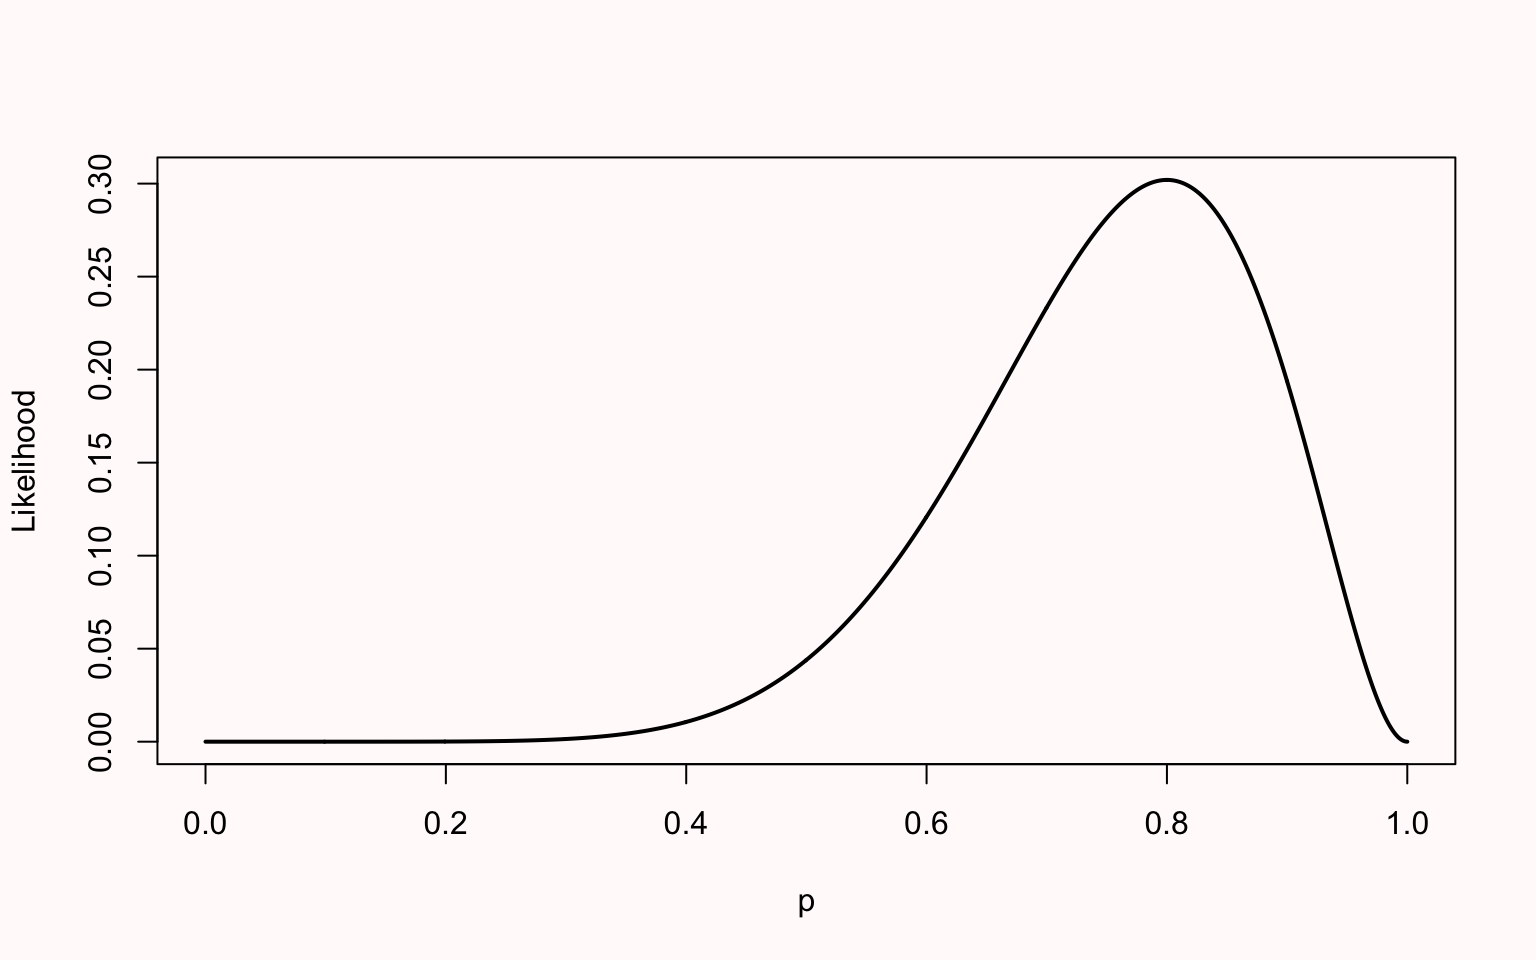
\includegraphics[width=1\linewidth]{03-likelihoods_files/figure-latex/like1-1} 

}

\caption{Binomial likelihood function for 8 successes in 10 trials.}\label{fig:like1}
\end{figure}

The likelihood is plotted for all possible values of \emph{p} (from 0 to 1). It should not be surprising that given the data we have observed, the most likely value for the true parameter is 8 out of 10, or \emph{p} = 0.8, with a likelihood of 0.30 (the highest point on the y-axis). In this example, \emph{p} = 0.8 is called the \textbf{maximum likelihood estimator}. It is important to know that the likelihood itself has no meaning in isolation. In this sense, it differs from a probability. But we can compare likelihoods of the same function across different values of \emph{p}. You can read off any other value for any other p, and see that given the observed data, low values of \emph{p} (e.g., 0.2) are not very likely.

There is a subtle difference between a probability and a likelihood. In colloquial language, you can use both terms to mean the same thing, but in statistics both terms used for different sides of the same coin. Note how the equation for Pr involves both information about the data (\emph{k}, \emph{n}) and information about the parameter (\emph{p}). To compute a \textbf{probability}, we view \emph{p} as fixed (for instance, for a fair coin, we plug in \emph{p} = 0.5) and then estimate the probability of different outcomes (\emph{k}, \emph{n}). The resulting function is the probability mass function. To compute the \textbf{likelihood}, we instead view the observed data as fixed (e.g., observing 5 heads out of 10 coin tosses), and we view Pr as a function of \emph{p}, estimating the value that maximizes the likelihood of a particular sample.

Likelihoods are an example of statistical inference: We have observed some data, and we use this data to draw an inference about different population parameters. More formally, the likelihood function is the (joint) density function evaluated at the observed data. Likelihood functions can be calculated for many different models (binomial distributions, normal distributions, see \citet{millar_maximum_2011}). This approach is called \textbf{likelihoodist statistics}, or \textbf{likelihoodism}, and it is distinct from frequentist and Bayesian approaches to statistics, as it directly used the likelihood function to make inferences.

When a mix of heads and tails has been observed, the likelihood curve rises and falls, as it is not possible that the coin can only come up heads or tails (after all, both have already been observed). If only heads of 0 heads are observed. When we plot the likelihood curves for 0 heads in 10 coin flips, the likelihood curve looks like Figure \ref{fig:like2}.



\begin{figure}

{\centering 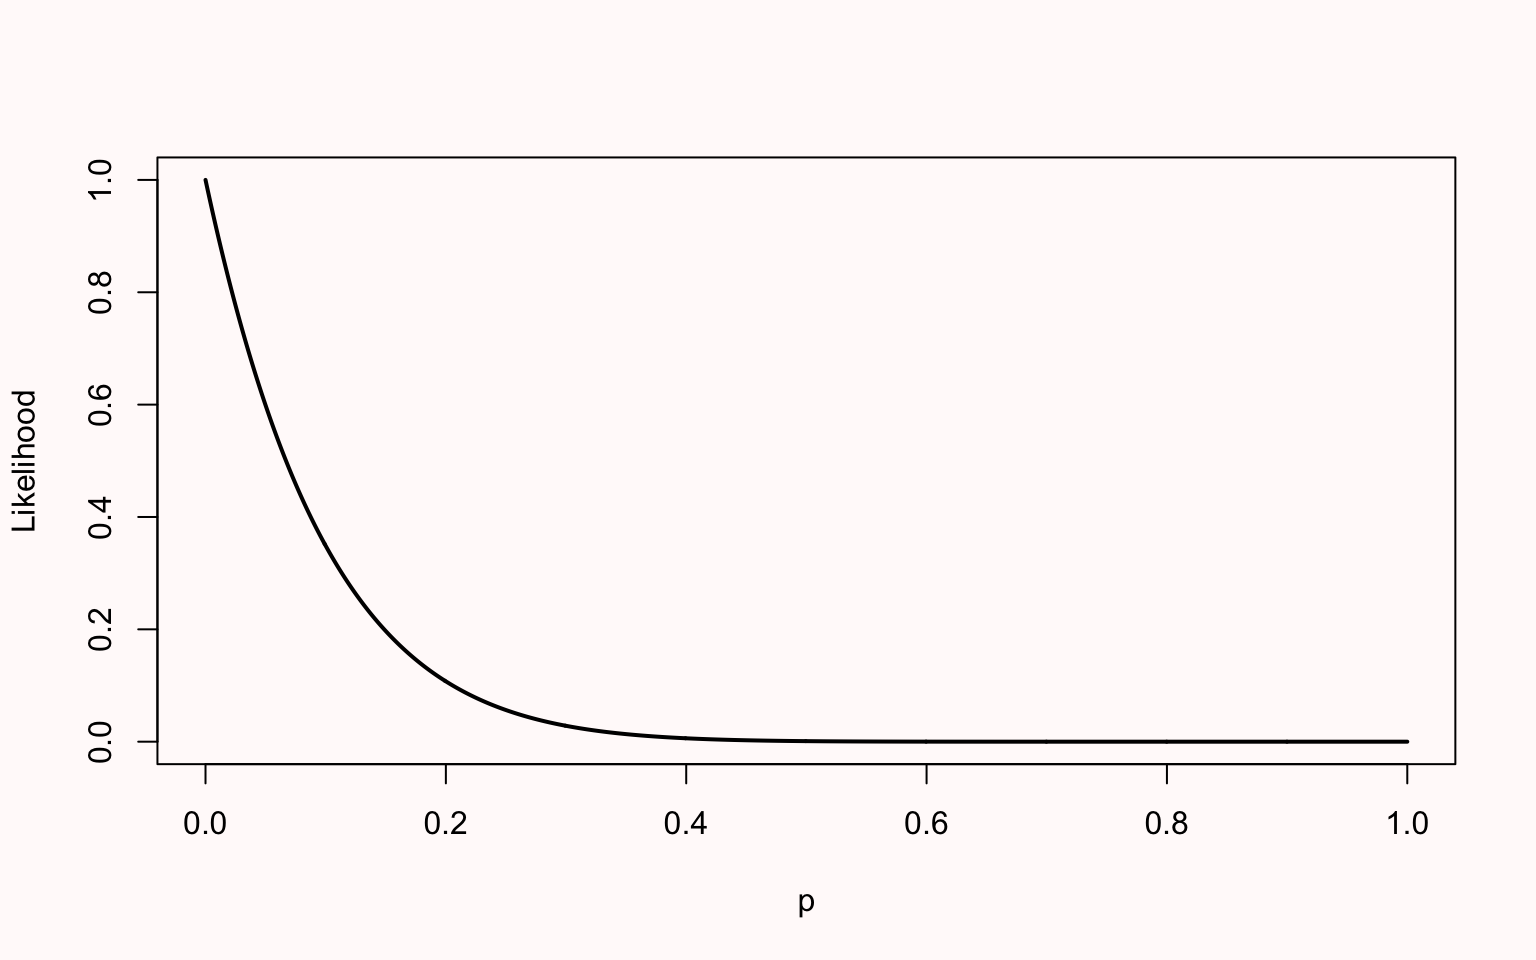
\includegraphics[width=1\linewidth]{03-likelihoods_files/figure-latex/like2-1} 

}

\caption{Binomial likelihood function for 0 successes in 10 trials.}\label{fig:like2}
\end{figure}

Likelihoods can easily be combined. Imagine we have two people flipping the same coin independently. One person observes 8 heads out of 10 flips, and the other observes 4 heads out of 10 flips. You might believe that this should give the same likelihood curve as one person flipping a coin 20 times, and observing 12 heads, and indeed, it does. In the plot below, all likelihood curves are standardized by dividing the curve by the maximum of each likelihood curve. This is why all curves now have a maximum of 1, and we can more easily compare different likelihood curves.



\begin{figure}

{\centering 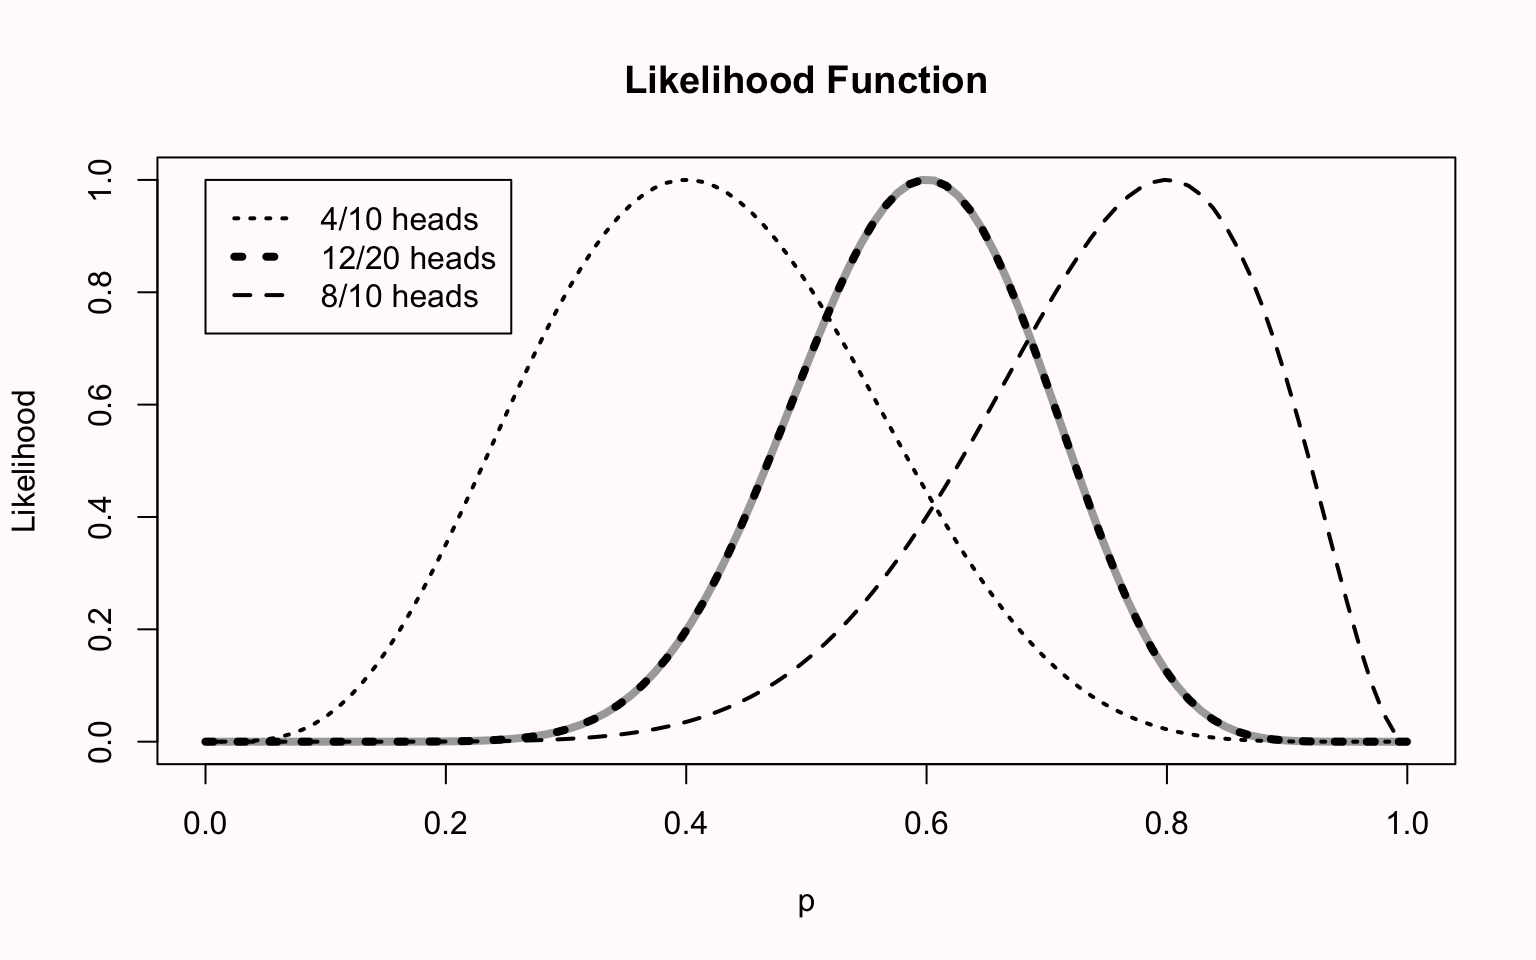
\includegraphics[width=1\linewidth]{03-likelihoods_files/figure-latex/like3-1} 

}

\caption{Combining likelihoods.}\label{fig:like3}
\end{figure}

The curve on left is for 4 out of 10 heads, the one on the right is for 8 out of 10 heads. The black dotted curve in the middle is for 12 out of 20 heads. The grey curve, exactly underneath the 12 out of 20 heads curve, is calculated by multiplying the likelihood curves: \(L(p_{combined}) = L(p = 0.8) / L(p = 0.4)\).

In Figure \ref{fig:like4} we see likelihood curves for 10, 100, and 1000 coin flips, which yield 5, 50, and 500 heads, respectively. The likelihood curves are again standardized to make them more easily comparable. As the sample size increases, the curves become more narrow (the dashed line is for \emph{n} = 10, the dotted line is for \emph{n} = 100, and the solid line is for \emph{n} = 1000). This means that as the sample size increases, our data become increasingly less likely under population parameters further removed from the observed number of heads. In other words, we have collected increasingly strong evidence for \emph{p} = 0.5, compared to most other possible population parameters.



\begin{figure}

{\centering 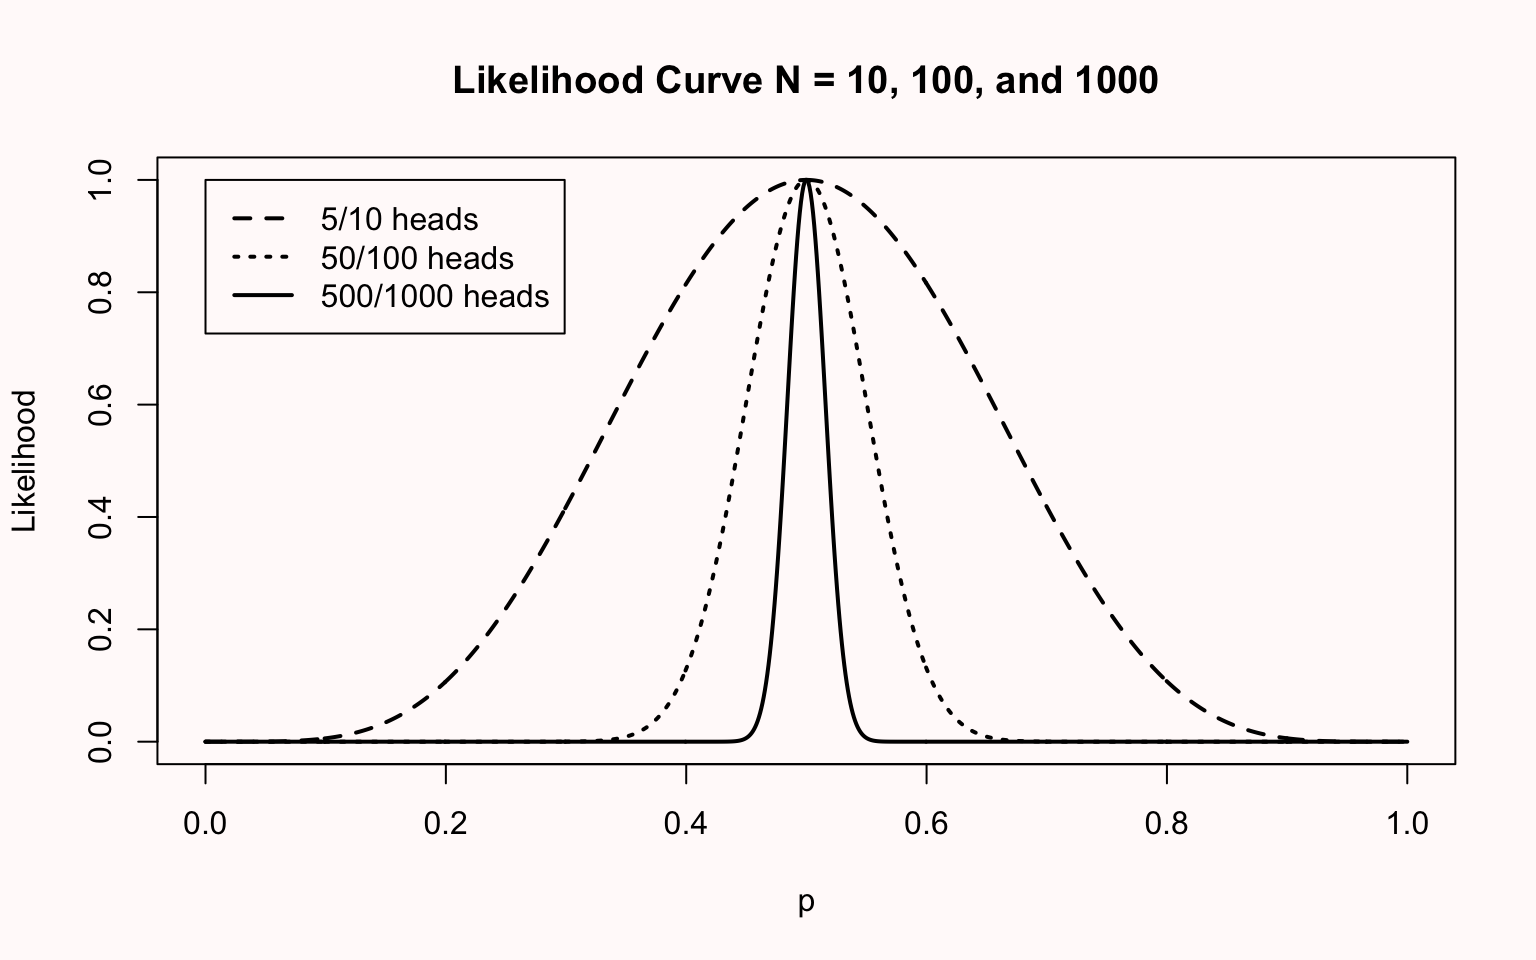
\includegraphics[width=1\linewidth]{03-likelihoods_files/figure-latex/like4-1} 

}

\caption{Likelihood function for 5/10, 50/100 and 500/1000 heads in coin flips.}\label{fig:like4}
\end{figure}

\hypertarget{likelihood-ratios}{%
\section{Likelihood ratios}\label{likelihood-ratios}}

We can use the likelihood function to compare possible values of p.~For example, we might believe the coin we flipped was fair, even though we flipped eight out of ten heads. A fair coin will have \emph{p} = 0.5, while we observed \emph{p} = 0.8. The likelihood function allows us to compute the relative likelihood for different possible parameters. How much more likely is our observed data under the hypothesis that this is an unfair coin that will on average turn up heads 80\% of the time, compared to the alternative theory that this is a fair coin which should turn up heads 50\% of the time?

We can calculate the likelihood ratio:

\[
\frac{L(p = 0.8)}{L(p = 0.5)}
\]

Which is 0.302/0.044 = 6.87. In the plot, both circles show the points on
the likelihood curve for L(\emph{p} = 0.5) and L(\emph{p} = 0.8).



\begin{figure}

{\centering 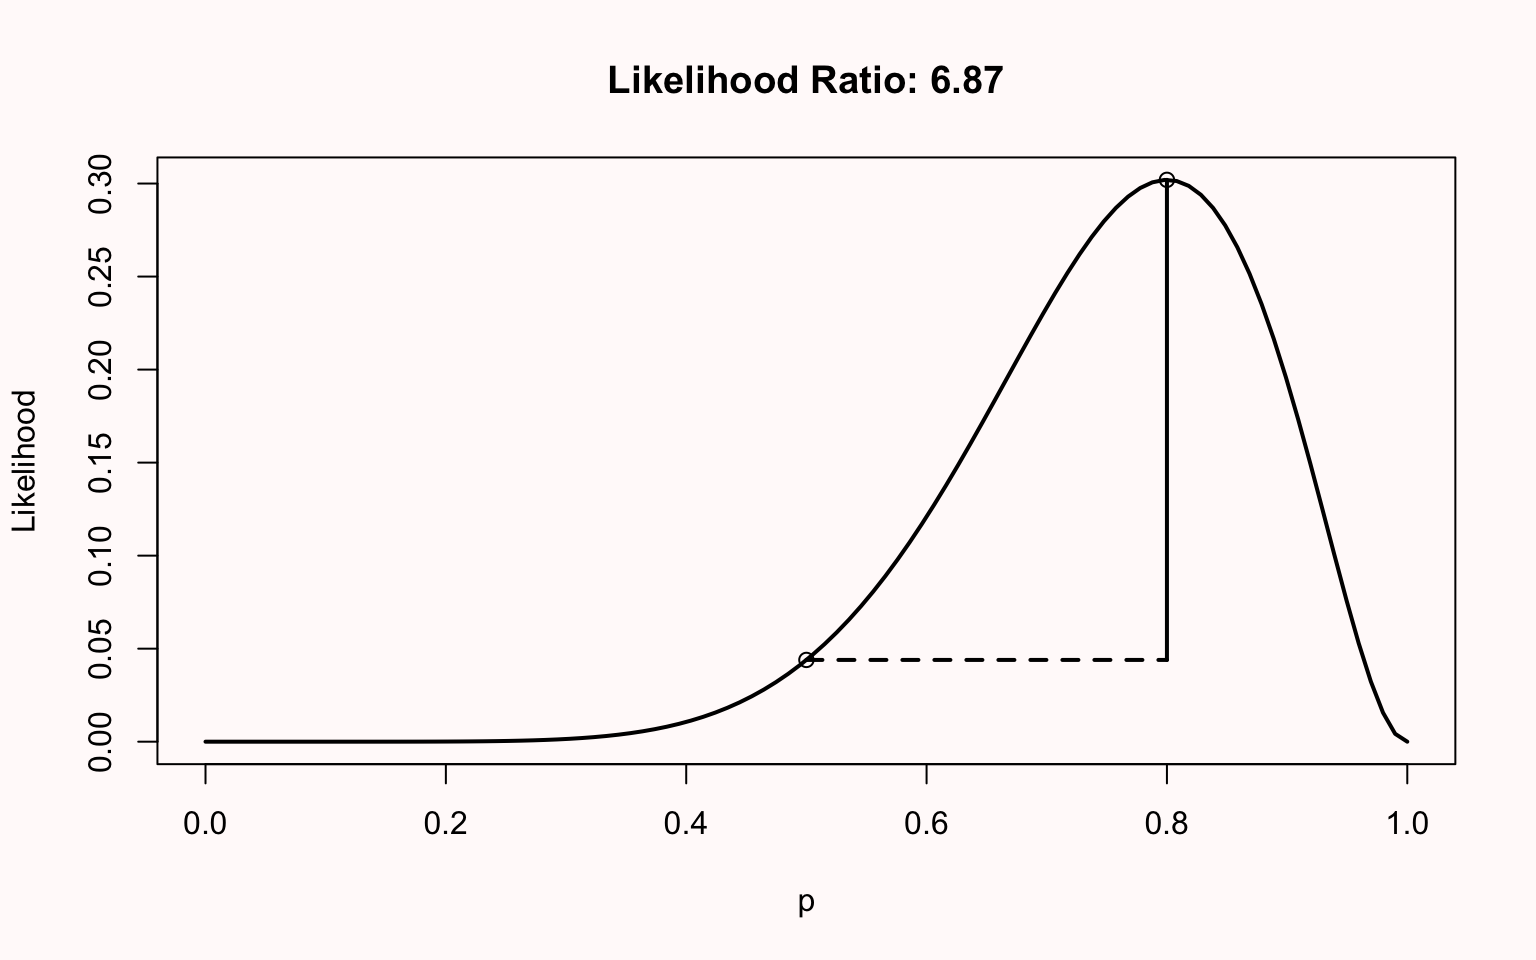
\includegraphics[width=1\linewidth]{03-likelihoods_files/figure-latex/like5-1} 

}

\caption{Computing a likelihood ratio for \emph{p} = 0.5 relative to \emph{p} = 0.8 when observing \emph{p} = 0.8.}\label{fig:like5}
\end{figure}

We can subjectively interpret this likelihood ratio, which tells us that our observed data is 6.87 times more likely under the hypothesis that this coin is unfair and will turn up heads 80\% of the time, than under the hypothesis that this is a fair coin. How convincing is this? Let's round the likelihood ratio to 7, and imagine two bags of marbles. One bag contains 7 blue marbles. The second contains 7 marbles, each one a different color of the rainbow, so violet, indigo, blue, green, yellow, orange, and red. Someone randomly picks one of the two bags, draws a marble, and shows it to you. The marble is blue: How certain are you this marble came from the bag with all blue marbles, compared to the bag with rainbow coloured marbles? This is how strong the likelihood ratio tells us to believe our data were generated by an unfair coin that turns up heads 80\% of the time, relative to a fair coin, given that we have observed 8 heads in 10 tosses. After this explanation intended to not make you rely too much on benchmarks, it might still be useful to know that \citet{royall_statistical_1997} considered likelihood ratios of 8 moderately strong evidence, and likelihood ratios of 32 strong evidence.

Note that likelihood ratios give us the relative evidence for one specified hypothesis, over another specified hypothesis. The likelihood ratio can be calculated for any two hypothesized values. For example, in Figure \ref{fig:like6} below, the likelihood ratio is calculated that compares the hypothesis for a fair coin (\emph{p} = 0.5) with the alternative hypothesis that the coin comes up heads 80\% of the time (\emph{p} = 0.8), when we have observed 4 heads out of 10 coin flips. We see that the observed data are 0.2050/0.0055=37.25 times more likely (ignoring rounding differences -- and try to calculate these numbers by hand using the formula provided earlier) under the hypothesis that this is a fair coin is than under the hypothesis that this is a coin that turns up heads 80\% of the time.



\begin{figure}

{\centering 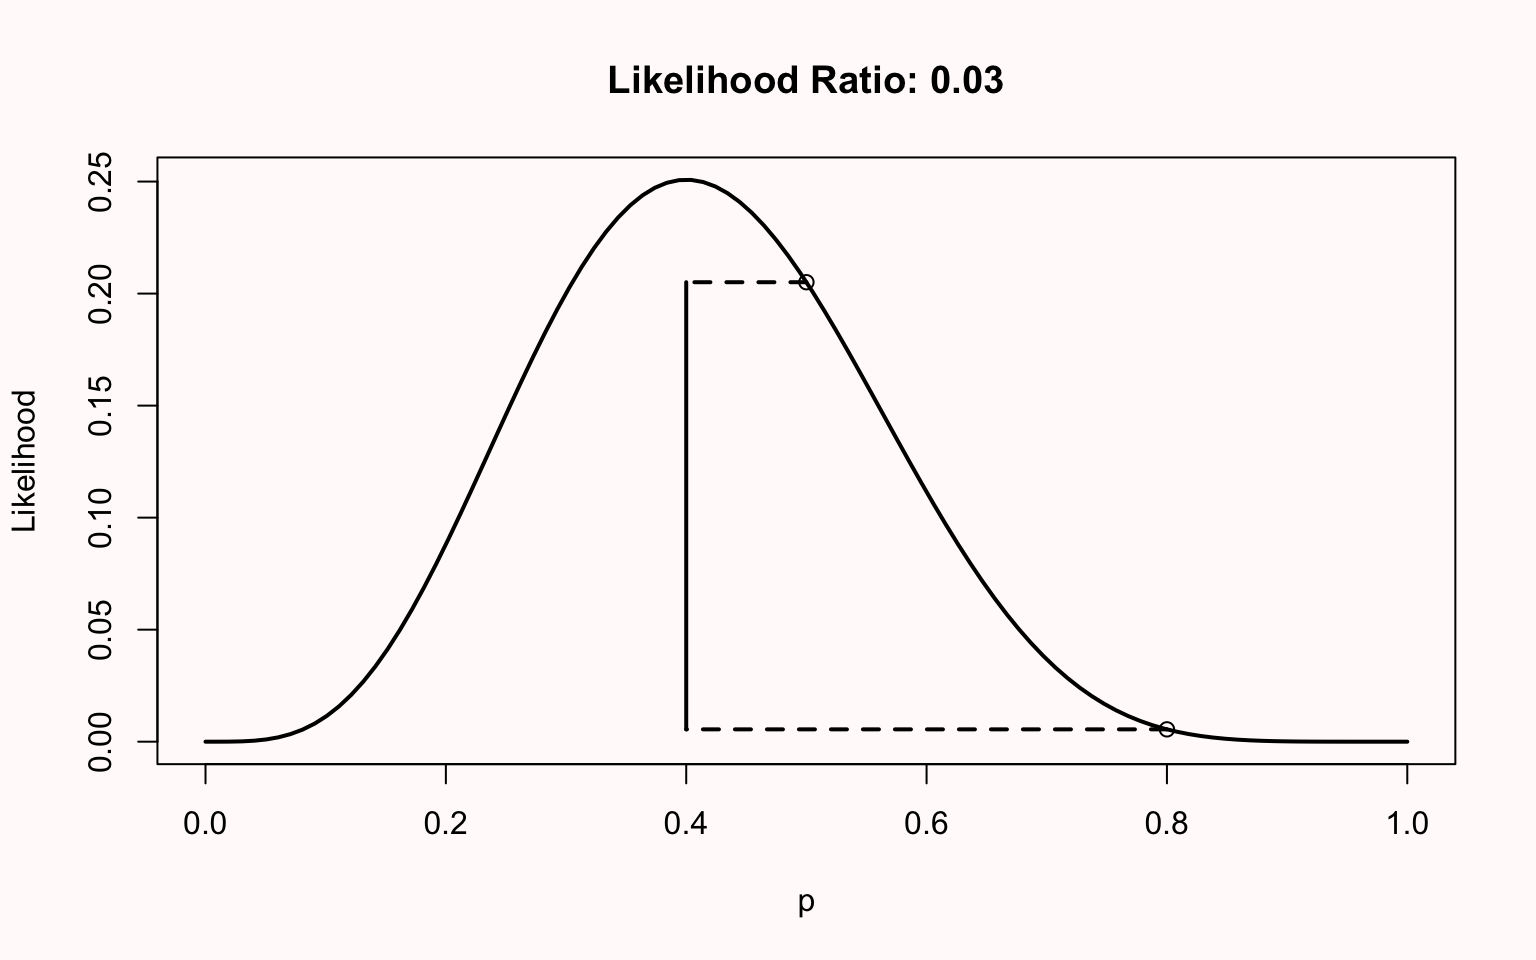
\includegraphics[width=1\linewidth]{03-likelihoods_files/figure-latex/like6-1} 

}

\caption{Computing a likelihood ratio for \emph{p} = 0.5 relative to \emph{p} = 0.8 when observing \emph{p} = 0.4.}\label{fig:like6}
\end{figure}

A likelihood ratio of 1 means the data are equally likely under both hypotheses. Values further away from 1 indicate that the data are more likely under one hypothesis than the other. The ratio can be expressed in favor of one hypothesis over the other (for example L(\emph{p} = 0.5)/L(\emph{p} = 0.8) or vice versa (L(\emph{p} = 0.8)/L(\emph{p} = 0.5). This means the likelihood ratio of 37.25 for \(H_0\) relative to \(H_1\) is equivalent to a likelihood ratio of 1/37.25 = 0.02685 for \(H_1\) relative to \(H_0\). Likelihood ratios range from 0 to infinity, and the closer to zero or infinity, the stronger the relative evidence for one hypothesis over the other. We will see in the chapter on \protect\hyperlink{bayes}{Bayesian statistics} that likelihood ratios are in this sense very similar (and a special case of) a Bayes Factor.

Likelihoods are relative evidence. Just because the data are more likely under one possible value of \emph{p} than another value of \emph{p} doesn't mean that the data have come from either of these two distributions. Other values might generate even higher likelihood values. For example, consider the situation where we flip a coin 100 times, and observe 50 heads. We compare \emph{p} = 0.3 versus \emph{p} = 0.8, and find that the likelihood ratio is 803462, implying that there is 803461 times more evidence in the data for \emph{p} = 0.3 than for \emph{p} = 0.8. That might sound pretty conclusive evidence for \emph{p} = 0.3. But it is only relative evidence for \emph{p} = 0.3 compared to \emph{p} = 0.8. If we look at the likelihood function, we clearly see that, not surprisingly, \emph{p} = 0.5 is the value that maximizes the likelihood function. Just because one hypothesis is more likely than another hypothesis, does not mean that there isn't a third hypothesis that is even more likely.



\begin{figure}

{\centering 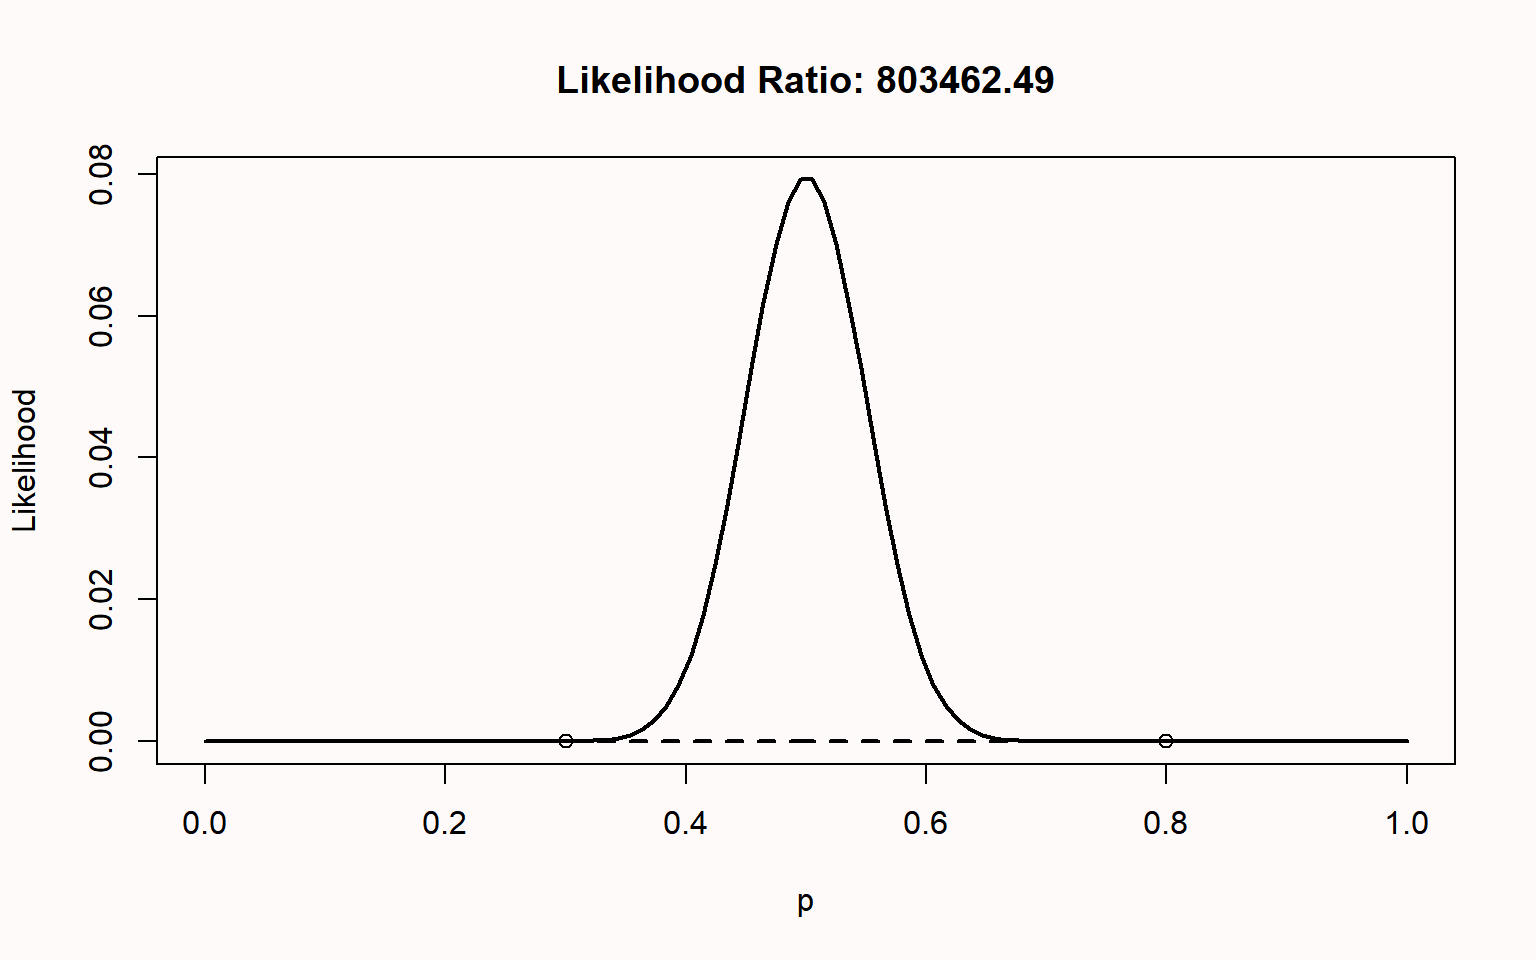
\includegraphics[width=1\linewidth]{03-likelihoods_files/figure-latex/like7-1} 

}

\caption{Computing a likelihood ratio for \emph{p} = 0.3 relative to \emph{p} = 0.8 when observing \emph{p} = 0.5 in 100 coin flips.}\label{fig:like7}
\end{figure}

\hypertarget{likelihood-of-mixed-results-in-sets-of-studies}{%
\section{Likelihood of mixed results in sets of studies}\label{likelihood-of-mixed-results-in-sets-of-studies}}

Science is a cumulative process, and we should evaluate lines of research, not single studies. One big problem in the scientific literature is that nonsignificant results are often never published \citep{franco_publication_2014, fanelli_positive_2010}. At the same time, because the statistical power of hypothesis tests are never 100\% (and often much lower), it is a mathematical reality that it is unlikely (or ``too good to be true'') that a set of multiple studies yields exclusively significant results. \citep{schimmack_ironic_2012, francis_frequency_2014}. We can use binomial likelihoods to examine how likely it is to observe mixed results, and understand when mixed results are nevertheless strong evidence for the presence of an effect. The following is largely based on \citet{lakens_too_2017}.

The probability of observing a significant or nonsignificant result in a study depends on the Type 1 error rate (\(\alpha\)), the statistical power of the test (1-\(\beta\)), and the probability that the null hypothesis is true \citep{wacholder_assessing_2004}. There are four possible outcomes of a study: a true positive, a false positive, a true negative, and a false negative. When \(H_0\) is true, the probability of observing a false positive depends on the \(\alpha\) level or the Type 1 error rate (e.g., 5\%). When \(H_1\) is true, the probability of observing a true positive depends on the statistical power of the performed test (where an often recommended minimum is 80\%), which in turn depends on the \(\alpha\) level, the true effect size, and the sample size. With an \(\alpha\) level of 5\%, and when \(H_0\) is true, a false positive will occur with a 5\% probability (as long as error rates are controlled, e.g., in preregistered studies) and true negative will occur with a 95\% probability. When a test has 80\% power, and \(H_1\) is true, a true positive has a probability of 80\%, and a false negative has a probability of 20\%.

If we perform multiple studies, we can calculate the binomial probability that we will observe a specific number of significant and nonsignificant findings \citep{ioannidis_exploratory_2007}. We can calculate the probability of finding exactly two significant results out of three studies assuming the null hypothesis is true. When \(H_0\) is true, the probability of significant results equals the \(\alpha\) level, and thus when the \(\alpha\) level is carefully controlled (e.g., in preregistered studies) \emph{p} = 0.05. When k = 2, n = 3, and \emph{p} = .05, the binomial probability function tells us that the probability of finding exactly two significant results in three studies is 0.007 (0.05 × 0.05 × 0.95 = 0.002375, and there are three orders in which two of the three results can be observed, so 0.002375 × 3 = 0.007).

To calculate the likelihood assuming \(H_1\) is true, we need to make an assumption about the power in each study. Let's provisionally assume all studies were powered at 80\% and thus \emph{p} = .80. The probability of observing exactly two significant results in three studies, assuming a power of 0.8, is 0.384 (0.8 × 0.8 × 0.2 = 0.128, and with three orders in which two of the three results can be significant, 0.128 × 3 = 0.384). In other words, if you set out to perform 3 studies, your hypothesis is correct, and you test your hypothesis with 80\% power, there is a 38.4\% probability of observing 2 out of 3 significant results, and a 9.6\% probability to observe 1 out of 3 significant results (and for an extremely unlucky individual, a 0.8\% probability of not finding any significant results in three studies, even though there is a true effect). Unless power is extremely high, mixed results should be expected in sets of studies.

Both likelihoods at \emph{p} = .05 and \emph{p} = .80 are highlighted in Figure \ref{fig:like8} by the circles on the dotted vertical lines.We can use the likelihood of the data assuming \(H_0\) or \(H_1\) is true to calculate the likelihood ratio, 0.384/0.007 = 53.89, which tells us the observed outcome of exactly two significant results out of three studies is 53.89 times more likely when \(H_1\) is true and studies had 80\% power, than when \(H_0\) is true and studies a carefully controlled 5\% Type 1 error rate. Likelihood ratios of 8 and 32 have been proposed as benchmarks of moderately strong and strong evidence, respectively \citep{royall_statistical_1997}, which implies that finding two significant results out of the three studies could be considered strong evidence for \(H_1\), assuming 80\% power. A Shiny app to perform these calculations is available \href{https://shiny.ieis.tue.nl/mixed_results_likelihood/}{here}.



\begin{figure}

{\centering 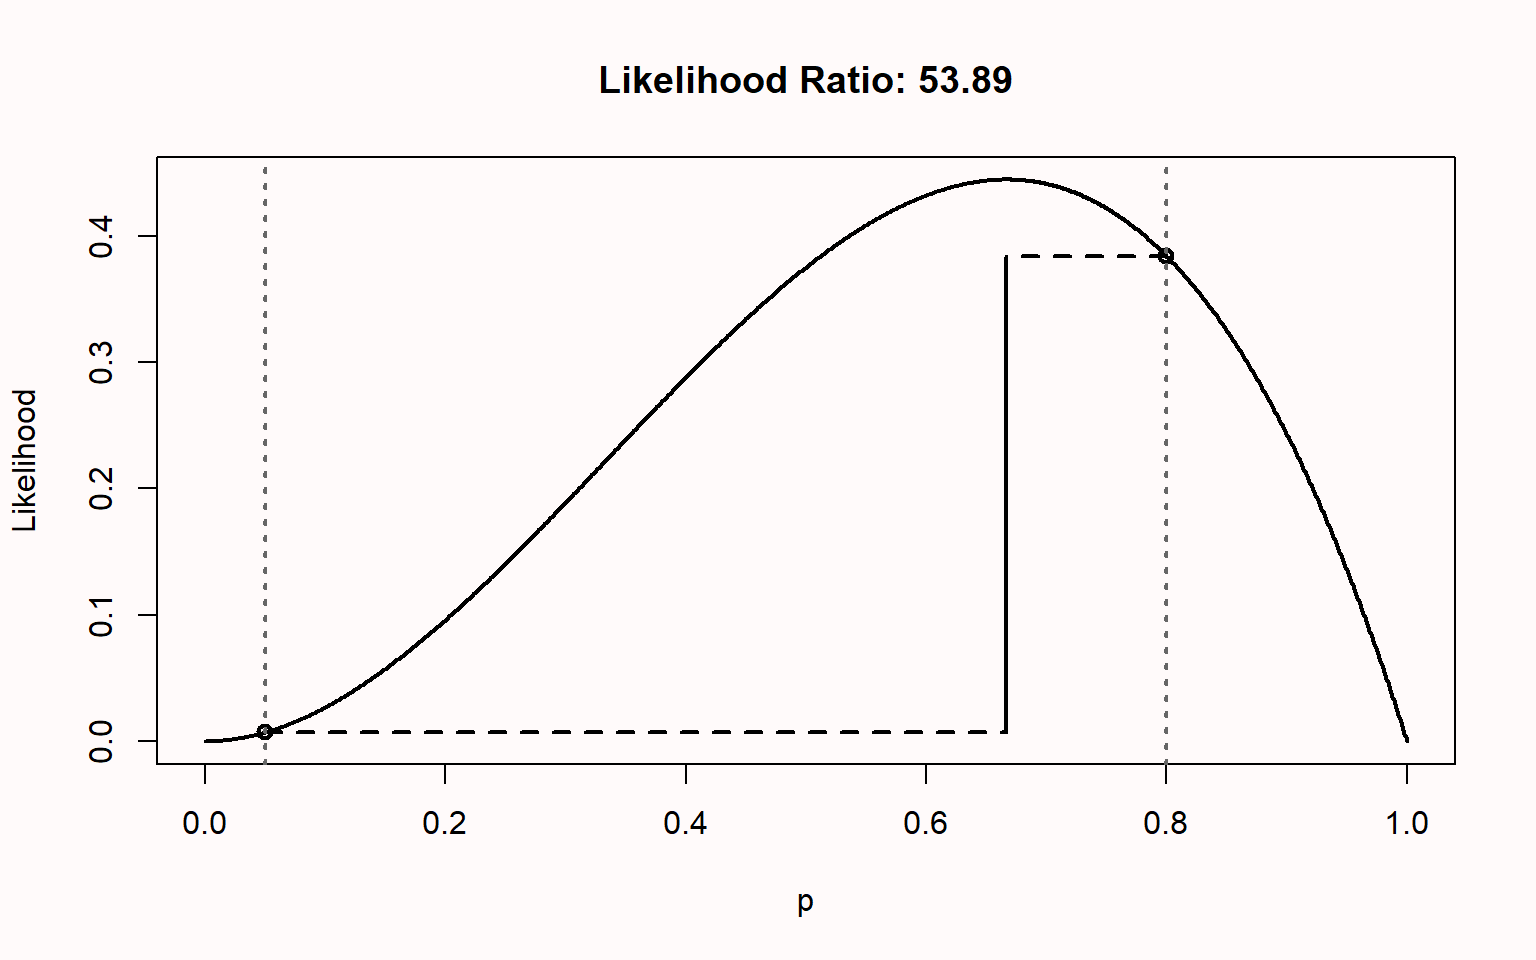
\includegraphics[width=1\linewidth]{03-likelihoods_files/figure-latex/like8-1} 

}

\caption{Computing a likelihood ratio for 2 out of three significant results, assuming an alpha of 5\% and 80\% power.}\label{fig:like8}
\end{figure}

In sets of studies, the likelihood ratio in favor of \(H_1\) versus H0 after observing a mix of significant and nonsignificant findings can become surprisingly large. Even though the evidence appears to be mixed, there is actually strong evidence in favor of a true effect. For example, when a researcher performs six studies with 80\% power and a 5\% a level and finds three significant outcomes and three nonsignificant outcomes, the cumulative likelihood ratio is convincingly large at 38-to-1 in favor of \(H_1\) to consider the set of studies strong evidence for a true effect. Intuitively, researchers
might not feel convinced by a set of studies where three out of six results were statistically significant. But if we do the math, we see that such a set of studies can be very strong evidence in favor of a true effect. A better understanding of these probabilities might be an important step in mitigating the negative effects of publication bias.

Hopefully, researchers become more inclined to submit nonsignificant findings for publication when they have a better understanding of the evidential value in lines of research with mixed results. Publishing all performed studies in lines of research will reduce publication bias, and increase the informational value of the data in the scientific literature. Expecting all studies in lines of research to be statistically significant is not reasonable, and it is important that researchers develop more realistic expectations if they are to draw meaningful inferences from lines of research. We don't have a very good feeling for what real patterns of studies look like, because we are continuously exposed to a scientific literature that does not reflect reality. Almost all multiple study papers in the scientific literature present only statistically significant results, even though this is unlikely given the power of these studies, and the probability that we would only study correct predictions \citep{scheel_excess_2021}. Educating researchers about binomial probabilities and likelihood ratios is a straightforward way to develop more realistic expectations about what research lines that contain evidential value in favor of \(H_1\) actually look like.

\hypertarget{likettest}{%
\section{\texorpdfstring{Likelihoods for \emph{t}-tests}{Likelihoods for t-tests}}\label{likettest}}

So far we have computed likelihoods for binomial probabilities, but likelihoods can be computed for any statistical model \citep{glover_likelihood_2004, pawitan_all_2001}. For example, we can compute the relative likelihood of observing a \emph{t}-value under the null and an alternative hypothesis (Figure \ref{fig:like9}). Of course, the observed data is most likely if we assume the observed effect equals the true effect, but examining the likelihood reveals that there are many alternative hypotheses that are relatively more likely than the null hypothesis. This also holds when observing nonsignificant results, which can be more likely under an alternative hypothesis of interest, than under the null hypothesis. This is a reason why it is incorrect to say that there is no effect when \emph{p} \textgreater{} \(\alpha\) (see \protect\hyperlink{misconception1}{\emph{p}-value misconception 1}).



\begin{figure}

{\centering 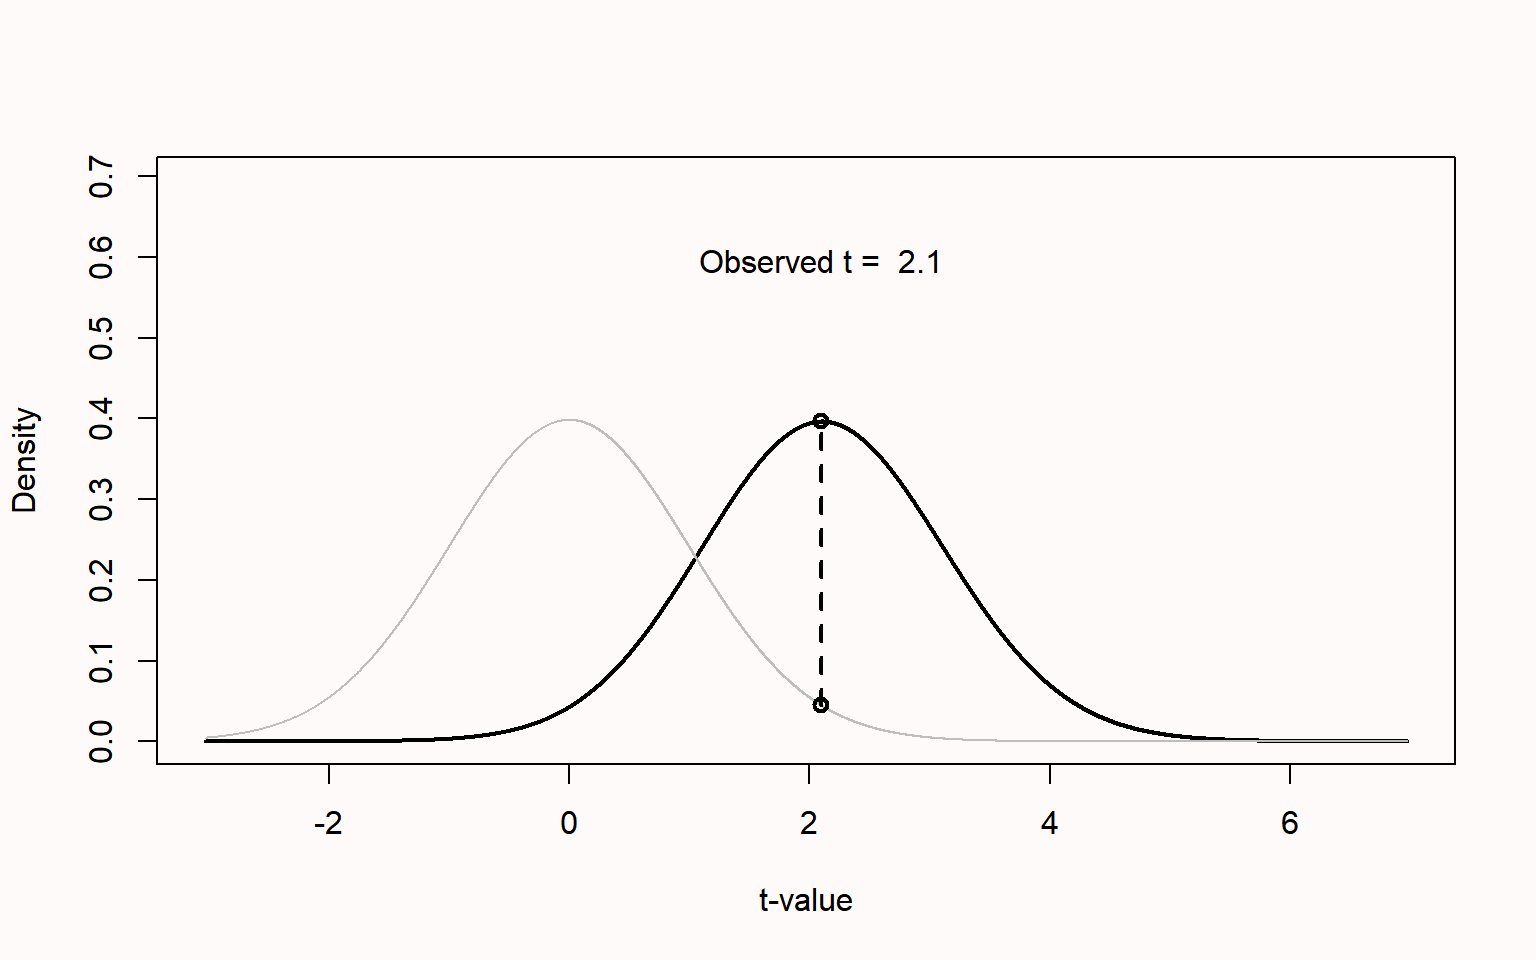
\includegraphics[width=1\linewidth]{03-likelihoods_files/figure-latex/like9-1} 

}

\caption{Likelihood ratio for observed \emph{t}-value under H0 and H1.}\label{fig:like9}
\end{figure}

\hypertarget{test-yourself-2}{%
\section{Test Yourself}\label{test-yourself-2}}

\hypertarget{questions-about-likelihoods}{%
\subsection{Questions about likelihoods}\label{questions-about-likelihoods}}

\textbf{Q1}: Let's assume you expect this is a fair coin. What is the binomial probability of observing 8 heads out of 10 coin flips, when p = 0.5? (You can use the functions in the chapter, or compute it by hand).

\begin{enumerate}
\def\labelenumi{\Alph{enumi})}
\tightlist
\item
  0.044
\item
  0.05
\item
  0.5
\item
  0.8
\end{enumerate}

\textbf{Q2}: The likelihood curve rises up and falls down, except at the extremes, when 0 heads or only heads are observed. Copy the code below (remember that you can click the `clipboard' icon on the top right of the code section to copy all the code to your clipboard), and plot the likelihood curves for 0 heads (x \textless- 0) out of 10 flips (n \textless- 10) by running the script. What does the likelihood curve look like?

\begin{Shaded}
\begin{Highlighting}[]
\NormalTok{n }\OtherTok{\textless{}{-}} \DecValTok{10} \CommentTok{\# set total trials}
\NormalTok{x }\OtherTok{\textless{}{-}} \DecValTok{5} \CommentTok{\# set successes}
\NormalTok{H0 }\OtherTok{\textless{}{-}} \FloatTok{0.5} \CommentTok{\# specify one hypothesis you want to compare}
\NormalTok{H1 }\OtherTok{\textless{}{-}} \FloatTok{0.4} \CommentTok{\# specify another hypothesis you want to compare}
\FunctionTok{dbinom}\NormalTok{(x, n, H0) }\SpecialCharTok{/} \FunctionTok{dbinom}\NormalTok{(x, n, H1) }\CommentTok{\# Returns the H0/H1 likelihood ratio}
\FunctionTok{dbinom}\NormalTok{(x, n, H1) }\SpecialCharTok{/} \FunctionTok{dbinom}\NormalTok{(x, n, H0) }\CommentTok{\# Returns the H1/H0 likelihood ratio}

\NormalTok{theta }\OtherTok{\textless{}{-}} \FunctionTok{seq}\NormalTok{(}\DecValTok{0}\NormalTok{, }\DecValTok{1}\NormalTok{, }\AttributeTok{len =} \DecValTok{100}\NormalTok{) }\CommentTok{\# create probability variable from 0 to 1}
\NormalTok{like }\OtherTok{\textless{}{-}} \FunctionTok{dbinom}\NormalTok{(x, n, theta)}

\FunctionTok{plot}\NormalTok{(theta, like, }\AttributeTok{type =} \StringTok{"l"}\NormalTok{, }\AttributeTok{xlab =} \StringTok{"p"}\NormalTok{, }\AttributeTok{ylab =} \StringTok{"Likelihood"}\NormalTok{, }\AttributeTok{lwd =} \DecValTok{2}\NormalTok{)}
\FunctionTok{points}\NormalTok{(H0, }\FunctionTok{dbinom}\NormalTok{(x, n, H0))}
\FunctionTok{points}\NormalTok{(H1, }\FunctionTok{dbinom}\NormalTok{(x, n, H1))}
\FunctionTok{segments}\NormalTok{(H0, }\FunctionTok{dbinom}\NormalTok{(x, n, H0), x }\SpecialCharTok{/}\NormalTok{ n, }\FunctionTok{dbinom}\NormalTok{(x, n, H0), }\AttributeTok{lty =} \DecValTok{2}\NormalTok{, }\AttributeTok{lwd =} \DecValTok{2}\NormalTok{)}
\FunctionTok{segments}\NormalTok{(H1, }\FunctionTok{dbinom}\NormalTok{(x, n, H1), x }\SpecialCharTok{/}\NormalTok{ n, }\FunctionTok{dbinom}\NormalTok{(x, n, H1), }\AttributeTok{lty =} \DecValTok{2}\NormalTok{, }\AttributeTok{lwd =} \DecValTok{2}\NormalTok{)}
\FunctionTok{segments}\NormalTok{(x }\SpecialCharTok{/}\NormalTok{ n, }\FunctionTok{dbinom}\NormalTok{(x, n, H0), x }\SpecialCharTok{/}\NormalTok{ n, }\FunctionTok{dbinom}\NormalTok{(x, n, H1), }\AttributeTok{lwd =} \DecValTok{2}\NormalTok{)}
\FunctionTok{title}\NormalTok{(}\FunctionTok{paste}\NormalTok{(}\StringTok{"Likelihood Ratio H0/H1:"}\NormalTok{, }\FunctionTok{round}\NormalTok{(}\FunctionTok{dbinom}\NormalTok{(x, n, H0) }\SpecialCharTok{/} \FunctionTok{dbinom}\NormalTok{(x, n, H1), }\AttributeTok{digits =} \DecValTok{2}\NormalTok{), }\StringTok{" Likelihood Ratio H1/H0:"}\NormalTok{, }\FunctionTok{round}\NormalTok{(}\FunctionTok{dbinom}\NormalTok{(x, n, H1) }\SpecialCharTok{/} \FunctionTok{dbinom}\NormalTok{(x, n, H0), }\AttributeTok{digits =} \DecValTok{2}\NormalTok{)))}
\end{Highlighting}
\end{Shaded}

\begin{enumerate}
\def\labelenumi{\Alph{enumi})}
\tightlist
\item
  The likelihood curve is a horizontal line.
\item
  The script returns and error message: it is not possible to plot the likelihood curve for 0 heads.
\item
  The curve starts at its highest point at p = 0, and then the likelihood decreases as p increases.
\item
  The curve starts at its lowest point at p = 0, and then the likelihood increases as p increases.
\end{enumerate}

\textbf{Q3}: Get a coin out of your wallet. Flip it 13 times, and count the number of heads. Using the code above, calculate the likelihood of your observed results under the hypothesis that your coin is fair, compared to the hypothesis that the coin is not fair. Set the number of successes (x) to the number of heads you observed. Change \(H_1\) to the number of heads you have observed (or leave it to 0 if you didn't observe any heads at all!). You can just use 4/13, or enter 0.3038. Leave \(H_0\) at 0.5. Run the script to calculate the likelihood ratio. What is the likelihood ratio of a fair compared to a non-fair coin (or \(H_0\)/\(H_1\)) that flips heads as often as you have observed, based on the observed data? Round your answer to 2 digits after the decimal.

Earlier we mentioned that with increasing sample sizes, we had collected stronger relative evidence. Let's say we would want to compare L(p = 0.4) with L(p = 0.5).

\textbf{Q4}: What is the likelihood ratio if \(H_1\) is 0.4, \(H_0\) is 0.5, and you flip 5 heads in 10 trials? From the two possible ways to calculate the likelihood ratio (\(H_1\)/\(H_0\) and \(H_0\)/\(H_1\)), report the likelihood that is ≥ 1, and round to 2 digits after the decimal point.

\textbf{Q5}: What is the likelihood ratio if \(H_1\) is 0.4, \(H_0\) is 0.5, and you flip 50 heads in 100 trials? From the two possible ways to calculate the likelihood ratio (\(H_1\)/\(H_0\) and \(H_0\)/\(H_1\)), report the likelihood that is ≥ 1, and round to 2 digits after the decimal point.

\textbf{Q6}: What is the likelihood ratio if \(H_1\) is 0.4, \(H_0\) is 0.5, and you flip 500 heads in 1000 trials? From the two possible ways to calculate the likelihood ratio (\(H_1\)/\(H_0\) and \(H_0\)/\(H_1\)), report the likelihood that is ≥ 1, and round to 2 digits after the decimal point.

\textbf{Q7}: When comparing two hypotheses (p = X vs p = Y), a likelihood ratio of:

\begin{enumerate}
\def\labelenumi{\Alph{enumi})}
\tightlist
\item
  0.02 means that there is not enough evidence in the data for either of the two hypotheses.
\item
  5493 means that hypothesis p = X is most supported by the data.
\item
  5493 means that hypothesis p = X is much more supported by the data than p = Y.
\item
  0.02 means that the hypothesis that the data are 2\% more likely under the hypothesis that p = X than under the hypothesis that p = Y.
\end{enumerate}

\hypertarget{questions-about-mixed-results}{%
\subsection{Questions about mixed results}\label{questions-about-mixed-results}}

\textbf{Q8:} Which statement is correct when you perform 3 studies?

\begin{enumerate}
\def\labelenumi{\Alph{enumi})}
\tightlist
\item
  When \(H_1\) is true, alpha = 0.05, and power = 0.80, it is almost as likely to observe one or more non-significant results (48.8\%) as it is to observe only significant results (51.2\%).
\item
  When alpha = 0.05 and power = 0.80, it is extremely rare that you will find 3 significant results (0.0125\%), regardless of whether \(H_0\) is true or \(H_1\) is true.
\item
  When alpha = 0.05 and power = 0.80, 2 out of 3 statistically significant results is the most likely outcome of all possible outcomes (0 out of 3, 1 out of 3, 2 out of 3, or 3 out of 3), and occurs 38.4\% of the time when \(H_1\) is true.
\item
  When alpha = 0.05 and power = 0.80, the probability of finding at least one false positive (a significant result when \(H_0\) is true) in three studies is 5\%.
\end{enumerate}

\textbf{Q9:} Sometimes in lines of three studies, you'll find a significant effect in one study, but there is no effect in the other two related studies. Assume the two related studies were not exactly the same in every way (e.g., you have changed the manipulation, or the procedure, or some of the questions). It could be that the two other studies did not work because of minor differences that had some effect you do not fully understand yet. Or it could be that the single significant result was a Type 1 error, and \(H_0\) was true in all three studies. Which statement below is correct, assuming a 5\% Type 1 error rate and 80\% power?

\begin{enumerate}
\def\labelenumi{\Alph{enumi})}
\tightlist
\item
  All else being equal, the probability of a Type 1 error in one of three studies is 5\% when there is no true effect in all three studies, and the probability of finding exactly 1 in three significant effects, assuming 80\% power in all three studies, is 80\%, which is substantially more likely.
\item
  All else being equal, the probability of a Type 1 error in one of three studies is 13.5\% when there is no true effect in all three studies, and the probability of finding exactly 1 in three significant effects, assuming 80\% power in all three studies (and thus a true effect), is 9.6\%, which is slightly, but not substantially less likely.
\item
  All else being equal, the probability of a Type 1 error in one of three studies is 85.7\% when there is no true effect in all three studies, and the probability of finding exactly 1 in three significant effects, assuming 80\% power in all three studies (and thus a true effect) (and thus a true effect), is 0.8\%, which is substantially less likely.
\item
  It is not possible to know the probability you will observe a Type 1 error if you perform 3 studies.
\end{enumerate}

The idea that most studies have 80\% power is slightly optimistic. \textbf{Examine the correct answer to the previous question across a range of power values} (e.g., 50\% power, and 30\% power).

\textbf{Q10:} Several papers suggest it is a reasonable assumption that the power in the psychological literature might be around 50\%. Set the number of studies to 4, the number of successes also to 4, and the assumed power slider to 50\%, and look at the table at the bottom of the app. How likely is it to observe 4 significant results in 4 studies, assuming there is a true effect?

\begin{enumerate}
\def\labelenumi{\Alph{enumi})}
\tightlist
\item
  6.25\%
\item
  12.5\%
\item
  25\%
\item
  37.5\%
\end{enumerate}

Imagine you perform 4 studies, and 3 show a significant result. \textbf{Change these numbers in the online app. Leave the power at 50\%}. The output in the text tells you:

\emph{When the observed results are equally likely under \(H_0\) and \(H_1\), the likelihood ratio is 1. Benchmarks to interpret Likelihood Ratios suggest that when 1\textless LR\textless8 there is weak evidence, when 8\textless LR\textless32 there is moderate evidence, and when LR\textgreater32, there is strong evidence.}

\emph{The data are more likely under the alternative hypothesis than the null hypothesis with a likelihood ratio of 526.32}

These calculations show that, assuming you have observed three significant results out of four studies, and assuming each study had 50\% power, it is 526 times more likely to have observed these data when the alternative hypothesis is true, than when the null hypothesis is true. In other words, it is 526 times more likely to find a significant effect in three studies when you have 50\% power, than to find three Type 1 errors in a set of four studies.

\textbf{Q11}: Maybe you don't think 50\% power is a reasonable assumption. How low can the power be (rounded to 2 digits), for the likelihood to remain higher than 32 in favor of \(H_1\) when observing 3 out of 4 significant results?

\begin{enumerate}
\def\labelenumi{\Alph{enumi})}
\tightlist
\item
  5\% power
\item
  17\% power
\item
  34\% power
\item
  44\% power
\end{enumerate}

The main take home message of these calculations is to understand that 1) mixed results are supposed to happen, and 2) mixed results can contain strong evidence for a true effect, across a wide range of plausible power values. The app also tells you how much evidence, in a rough dichotomous way, you can expect. This is useful for our educational goal. But when you want to evaluate results from multiple studies, the formal way to do so is by performing a meta-analysis.

The above calculations make a very important assumption: The Type 1 error rate is controlled at 5\%. If you try out many different tests in each study, and only report the result that yielded a p \textless{} 0.05, these calculations no longer hold.

\textbf{Q12}: Go back to the default settings of 2 out of 3 significant results, but now set the Type 1 error rate to 20\%, to reflect a modest amount of p-hacking. Under these circumstances, what is the \textbf{highest} likelihood in favor of \(H_1\) you can get if you explore all possible values for the true power?

\begin{enumerate}
\def\labelenumi{\Alph{enumi})}
\tightlist
\item
  Approximately 1
\item
  Approximately 4.63
\item
  Approximately 6.70
\item
  Approximately 62.37
\end{enumerate}

As the scenario above shows, \emph{p}-hacking makes studies extremely uninformative.
\textbf{If you inflate the error rate, you quickly destroy the evidence in the data.} You can no longer determine whether the data is more likely when there is no effect, than when there is an effect. Sometimes researchers complain that people who worry about \emph{p}-hacking and try to promote better Type 1 error control are missing the point, and that other things (better measurement, better theory, etc.) are more important. I fully agree that these aspects of scientific research are at least as important as better error control. But better measures and theories will require decades of work. Better error control can be accomplished today, if researchers would stop inflating their error rates by flexibly analyzing their data. And as this assignment shows, inflated rates of false positives very quickly make it difficult to learn what is true from the data we collect. Because of the relative ease with which this part of scientific research can be improved, and because we can achieve this today (and not in a decade) I think it is worth stressing the importance of error control, and publish more realistic looking sets of studies.

\textbf{Q13}: Some `prestigious' journals (which, when examined in terms of scientific quality such as reproducibility, reporting standards, and policies concerning data and material sharing, are quite low quality despite their prestige) only publish manuscripts with a large number of studies, which should all be statistically significant. If we assume an average power in psychology of 50\%, only 3.125\% of 5 study articles should contain exclusively significant results. If you pick up a random issue from such a prestigious journal, and see 10 articles, each reporting 5 studies, and all manuscripts have exclusively significant results, would you trust the reported findings more, or less, than when all these articles had reported mixed results? Why?

\textbf{Q14}: Unless you will power all your studies at 99.99\% for the rest of your career (which would be slightly inefficient, but great if you don't like insecurity), you will observe mixed results in lines of research. How do you plan to deal with mixed results in lines of research?

\hypertarget{open-questions-2}{%
\subsection{Open Questions}\label{open-questions-2}}

\begin{enumerate}
\def\labelenumi{\arabic{enumi}.}
\item
  What is the difference between a probability and a likelihood?
\item
  Why is it important to remember that a likelihood ratio is relative evidence?
\item
  If we compare 2 hypotheses, H0 and H1, and the likelihood ratio of H1 compared to H0 is 77, what does this mean?
\item
  What are benchmarks for medium and strong evidence according to Royall?
\item
  How can it be that a likelihood ratio is 200, but both hypotheses are incorrect?
\item
  If we perform multiple studies and find 2 out of 3 studies show a significant results, how can this actually be strong evidence for H1?
\end{enumerate}

\hypertarget{bayes}{%
\chapter{Bayesian statistics}\label{bayes}}

\begin{quote}
``Logic!'' said the Professor half to himself. ``Why don't they teach logic at these schools? There are only three possibilities. Either your sister is telling lies, or she is mad, or she is telling the truth. You know she doesn't tell lies and it is obvious that she is not mad. For the moment then and unless any further evidence turns up, we must assume that she is telling the truth.''
\end{quote}

\emph{\href{https://gutenberg.ca/ebooks/lewiscs-thelionthewitchandthewardrobe/lewiscs-thelionthewitchandthewardrobe-00-h.html}{The Lion, The Witch, and The Wardrobe. A Story for Children} by C. S. Lewis.}

In the children's book The Lion, The Witch, and The Wardrobe, both Lucy and Edmund go through a wardrobe into a country called Narnia. Lucy tells her older brother and sister, Peter and Susan, about Narnia, but Edmund wants to keep it a secret, and tells Peter and Susan he and Lucy were just pretending Narnia exists. Peter and Susan don't know what to believe - does Narnia exist, or not? Is Lucy telling the truth, or is Edmund? Thinking about probabilities in the long run will not help much - this is a unique event, and we will need to think about the probability that Narnia exists, or not, based on the information we have available.

They ask the Professor, who lives in the house with the wardrobe, for advice. The Professor asks Susan and Peter if in their past experience, Lucy or Edward has been more truthful, to which Peter answers ``Up till now, I'd have said Lucy every time.'' So, they have a stronger prior belief Lucy is telling the truth, relative to Edward telling the truth. The Professor then replies with the quote above. From the three possible options, we don't believe Lucy is lying, as she has not done so in the past, and the Professor believes it is clear just from talking to Lucy that she is not mad. Therefore, the most plausible option is that Lucy is telling the truth. If new evidence is uncovered, these beliefs can be updated in the future. This approach to knowledge generation, where the prior probability of different hypotheses is quantified, and if possible updated in light of new data, is an example of \emph{Bayesian inference}.

Although frequentist statistics is by far the dominant approach in science, it is important to have had at least rudimentary exposure to Bayesian statistics during any statistics training. Bayesian statistics is especially useful when inferences are made in cases where the data under investigation is unique, and there is no frequentist probability defined as the limit in many trials. For example, the question might not be how often Lucy lies on average, but whether Lucy is lying in this specific instance about the existence of Narnia. When we do research, we often start with a prior belief that a hypothesis is true. After collecting data, we can use this data to update our prior beliefs. Bayesian statistics allows you to update prior beliefs into posterior probabilities in a logically consistent manner. Before we have collected data, the \textbf{prior odds} of Hypothesis 1 (\(H_1\)) over the null-hypothesis (\(H_0\)) are P(\(H_1\))/P(\(H_0\)), After we have collected data, we have the \textbf{posterior odds} P(\(H_1\)\textbar D)/P(\(H_0\)\textbar D), which you can read as the probability of \(H_1\), given the data, divided by the probability of \(H_0\), given the data. There are different approaches to Bayesian statistics. We will first discuss Bayes factors, and then Bayesian estimation.

\hypertarget{bayes-factors}{%
\section{Bayes factors}\label{bayes-factors}}

One approach in Bayesian statistics focuses on the comparison of different models that might explain the data (referred to as \textbf{model comparison}). In Bayesian statistics, the probability of data under a specified model (P\textbar D(\(H_0\)) is a number that expressed what is sometimes referred to as the absolute \textbf{evidence}, and more formally referred to as a marginal likelihood. The marginal likelihood uses prior probabilities to average the likelihood across the parameter space. For example, assume we have a simple model \emph{M} that is based on a single parameter, that can take on two values, X and Y, and that a-prior we believe the probability of both values is p(X) = 0.4 and p(Y) = 0.6. We collect data, and calculate the likelihood for both these parameter values, which is p(D\textbar X) = 0.02 and p(D\textbar Y) = 0.08. The marginal likelihood of our model \emph{M} is then P(D\textbar M) = 0.4 × 0.02 + 0.6 × 0.08 = 0.056. Most often, models have continuously varying parameters, and the marginal likelihood formula is based on an integral, but the idea remains the same.

A comparison of two models is based on the relative evidence the data provides for each models we are comparing. The relative evidence is calculated by dividing the marginal likelihood for one model by the marginal likelihood for another model, and this ratio of relative evidence based on these marginal likelihoods is called the \textbf{Bayes factor}. Bayes factors are the Bayesian equivalent of hypothesis tests \citep{dienes_understanding_2008, kass_bayes_1995}. The Bayes factor represents how much we have updated our beliefs, based on observing the data. We can express Bayes factors to indicate how much more likely \(H_1\) is given the data compared to \(H_0\) (often indicated by B10) or as how much more likely \(H_0\) has become compared to \(H_1\) (B01), and B10 = 1/B01. Similar to likelihood ratios of 1, a Bayes factor of 1 did not change our beliefs for one model compared to the other model. A very large Bayes factor for \(H_1\) over \(H_0\) has increased our belief in \(H_1\), and a Bayes Factor close for \(H_1\) over \(H_0\) to 0 has increased our belief in \(H_0\). If our prior belief in \(H_1\) was very, very low (e.g., your belief in unicorns) even a large Bayes factor that supports the presence of a unicorn might not yet convince you that unicorns are real -- but you have updated your belief in unicorns, and now believe they are at least more likely then they were before (even if you still think unicorns are very unlikely to exist). The contribution of the Bayes Factor and the prior in calculating the posterior odds is clear in the following formula:

\[
\frac{P(H_1|D)}{P(H_0|D)} = \ \frac{P(D|H_1)}{P(D|H_0)}\  \times \ \frac{P(H_1)}{P(H_0)}
\]

\[
Posterior\ Probability = \ Bayes\ Factor\  \times \ Prior\ Probability
\]

A Bayesian analysis of data requires specifying the prior. Here, we will continue our example based on a binomial probability, such as a coin flip. In the likelihood example, we compared two point hypotheses (e.g., \emph{p} = 0.5 vs.~\emph{p} = 0.8). In Bayesian statistics, parameters are considered to be random variables, and the uncertainty or degree of belief with respect to the parameters is quantified by \textbf{probability distributions}.

A binomial probability lies between 0 and 1. You could draw any probability density you want over 0 and 1, and turn it into a prior, but for good reasons (simplicity, mostly) a beta-prior is often used for binomial probabilities. The shape of the beta-prior depends on two parameters, \(\alpha\) and \(\beta\). Note that these are the same Greek letters as used for the Type 1 error rate and Type 2 error rate, but that is purely coincidental! The \(\alpha\) and \(\beta\) in binomial probabilities are unrelated to error rates, and the use of the same letters is mainly due to a lack of creativity among statisticians and the limited choice the alphabet gives us. It also does not help that \(\beta\) is one of the parameters of the Beta distribution. Try to keep these different Beta's apart! The probability density function is:

\[
\int_{}^{}{\left( x,\ \alpha,\ \beta \right) = \ \frac{1}{B(\alpha,\beta)}}x^{\alpha - 1}{(1 - x)}^{\beta - 1}
\]

where \emph{B(\(\alpha\), \(\beta\))} is the beta function. Understanding the mathematical basis of this function is beyond the scope of this chapter, but you can read more on \href{https://en.wikipedia.org/wiki/Beta_distribution}{Wikipedia} or Kruschke's book on Doing Bayesian Data Analysis \citep{kruschke_doing_2014}. The beta-prior for a variety of values for \(\alpha\) and \(\beta\) can be seen in the figure below.



\begin{figure}

{\centering 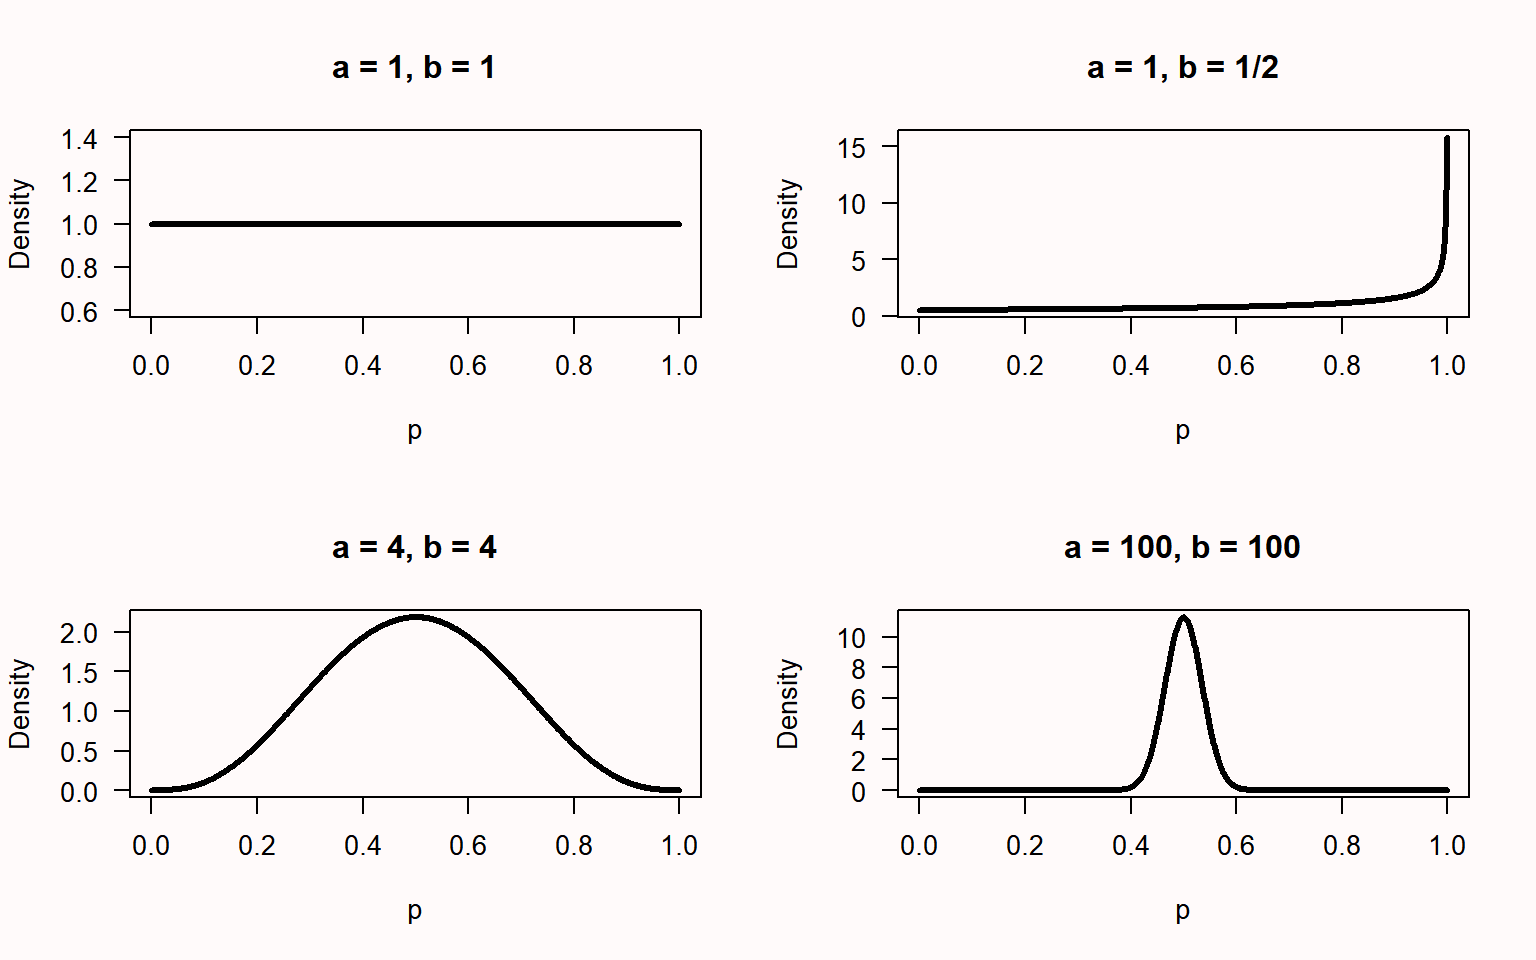
\includegraphics[width=1\linewidth]{04-bayes_files/figure-latex/bayes1-1} 

}

\caption{Four examples of Bayesian priors.}\label{fig:bayes1}
\end{figure}

These beta densities reflect different types of priors. Let's assume you are approached by a street merchant who tries to sell you a special coin with heads and tails that, when flipped, will almost always turn up heads. The \(\alpha\) = 1, \(\beta\) = 1 prior is what a newborn baby would have as a prior, without any idea of what to expect when you flip a coin, and thus every value of \emph{p} is equally likely. The \(\alpha\) = 1, \(\beta\) = 1/2 prior is what a true believer would have as a prior. The sales merchant tells you the coin will turn up heads almost every time, and thus, you believe it will turn up heads almost every time. The \(\alpha\) = 4, \(\beta\) = 4, and the \(\alpha\) = 100, \(\beta\) = 100 priors are for slightly and extremely skeptical people. With an \(\alpha\) = 4, \(\beta\) = 4 prior, you expect the coin will be fair, but you are willing to believe a wide range of other true values is possible (the curve is centered on 0.5, but the curve is wide, allowing for very high and low values of \emph{p}). With the \(\alpha\) = 100, \(\beta\) = 100 prior you are really convinced coins are fair, and believe there will be only a very slight bias, at most (the curve is again centered on 0.5, and a skeptic believes the \emph{p} will lie between 0.4 and 0.6 -- a much narrower range compared to the slightly skeptic individual).

Let's assume the newborn baby, the true believer, the slightly skeptic and the extreme skeptic all buy the coin, flip it n = 20 times, and observe x = 10 heads. This outcome can be plotted as a binomial distribution with 10 heads out of 20 trials, or as a Beta(11, 11) distribution.

The newborn baby had a prior Beta distribution with \(\alpha\) = 1 and \(\beta\) = 1, which equals a binomial likelihood distribution for 0 heads out of 0 trials. The posterior is a Beta distribution with Beta(\(\alpha\)*, \(\beta\)*), where:

\(\alpha\)* = \(\alpha\) + x = 1 + 10= 11

\(\beta\)* = \(\beta\) + n -- x = 1 + 20 -- 10 = 11

Or calculating these values more directly from the \(\alpha\) and \(\beta\) of the prior and
likelihood:

\(\alpha\)* = \(\alpha\)prior + \(\alpha\)likelihood -- 1 = 1 + 11 - 1= 11

\(\beta\)* = \(\beta\)prior + \(\beta\)likelihood - 1 = 1 + 11 -- 1 = 11

Thus, the posterior distribution for the newborn is a Beta(11,11) distribution. This equals a binomial likelihood function for 10 heads out of 20 trials, or Beta(11,11) distribution. In other words, the posterior distribution is identical to the likelihood function when a uniform prior is used.

Take a look at the Figure below. Given 10 heads out of 20 coin flips, we see the prior distribution of the newborn (the horizontal grey line), the likelihood (the blue dotted line) and the posterior (the black line).



\begin{figure}

{\centering 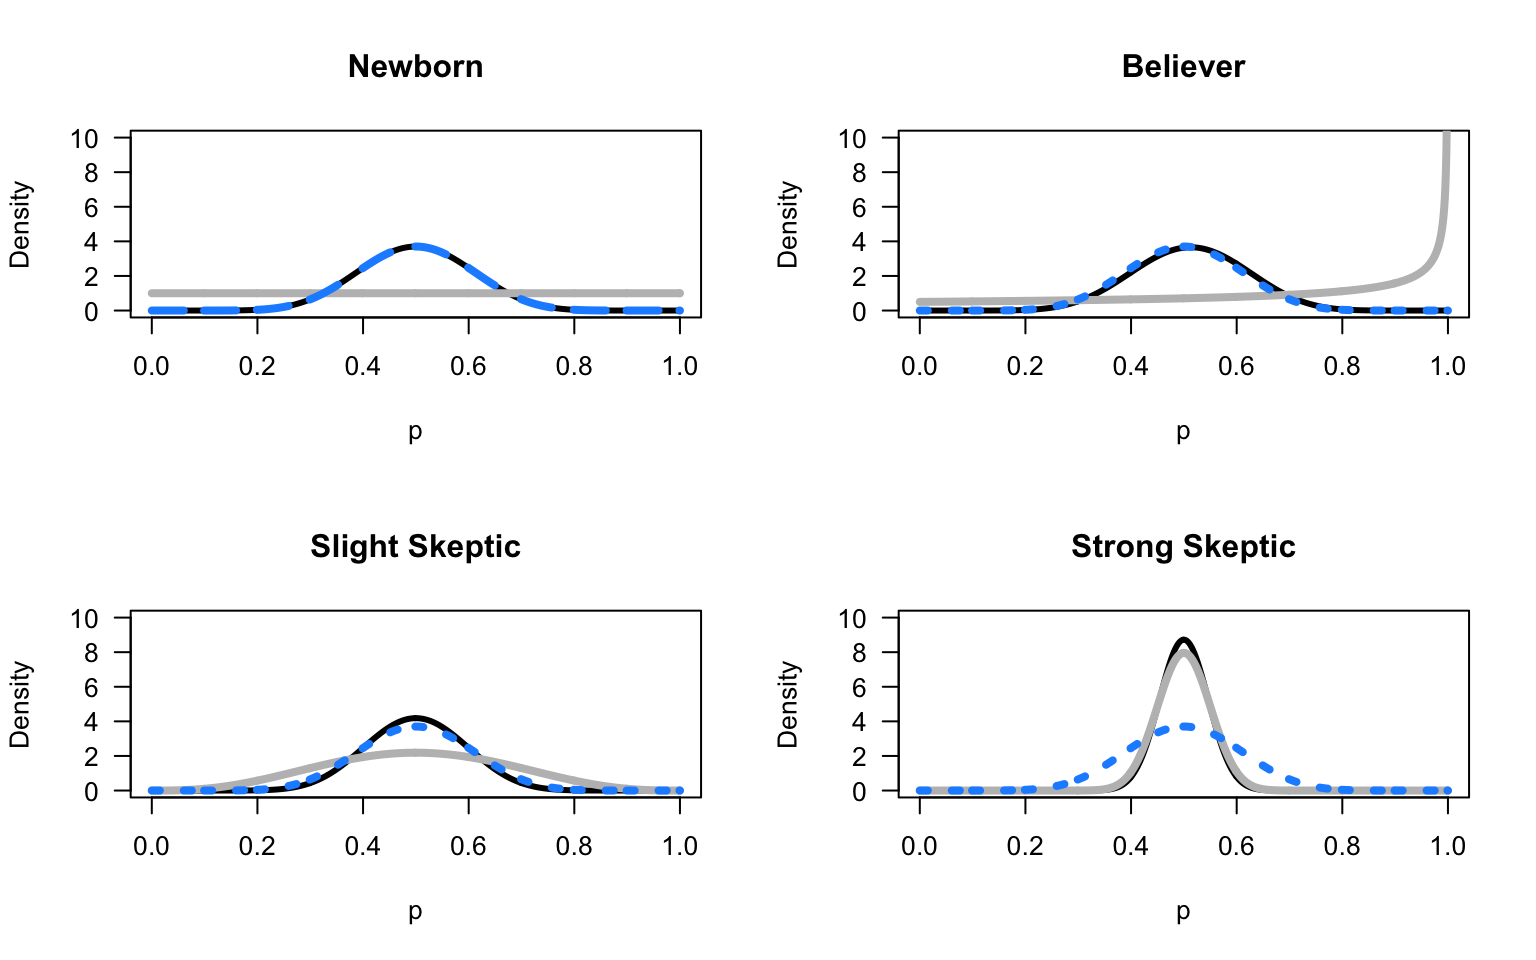
\includegraphics[width=1\linewidth]{04-bayes_files/figure-latex/bayes2-1} 

}

\caption{Four examples of how different priors are updated based on data to the posterior.}\label{fig:bayes2}
\end{figure}

For the true believer the posterior distribution is not centered on the maximum likelihood of the observed data, but just a bit in the direction of the prior. The slightly skeptic and the strong skeptic end up with a much stronger belief in a fair coin after observing the data, but mainly because they already had a stronger prior that the coin was fair.

\hypertarget{updating-our-belief}{%
\section{Updating our belief}\label{updating-our-belief}}

Now that we have a distribution for the prior, and a distribution for the posterior, we can see in the graphs below for which values of \emph{p} our belief has increased. Everywhere where the black line (of the posterior) is higher than the grey line (of the prior) our belief in that \emph{p} has increased.



\begin{figure}

{\centering 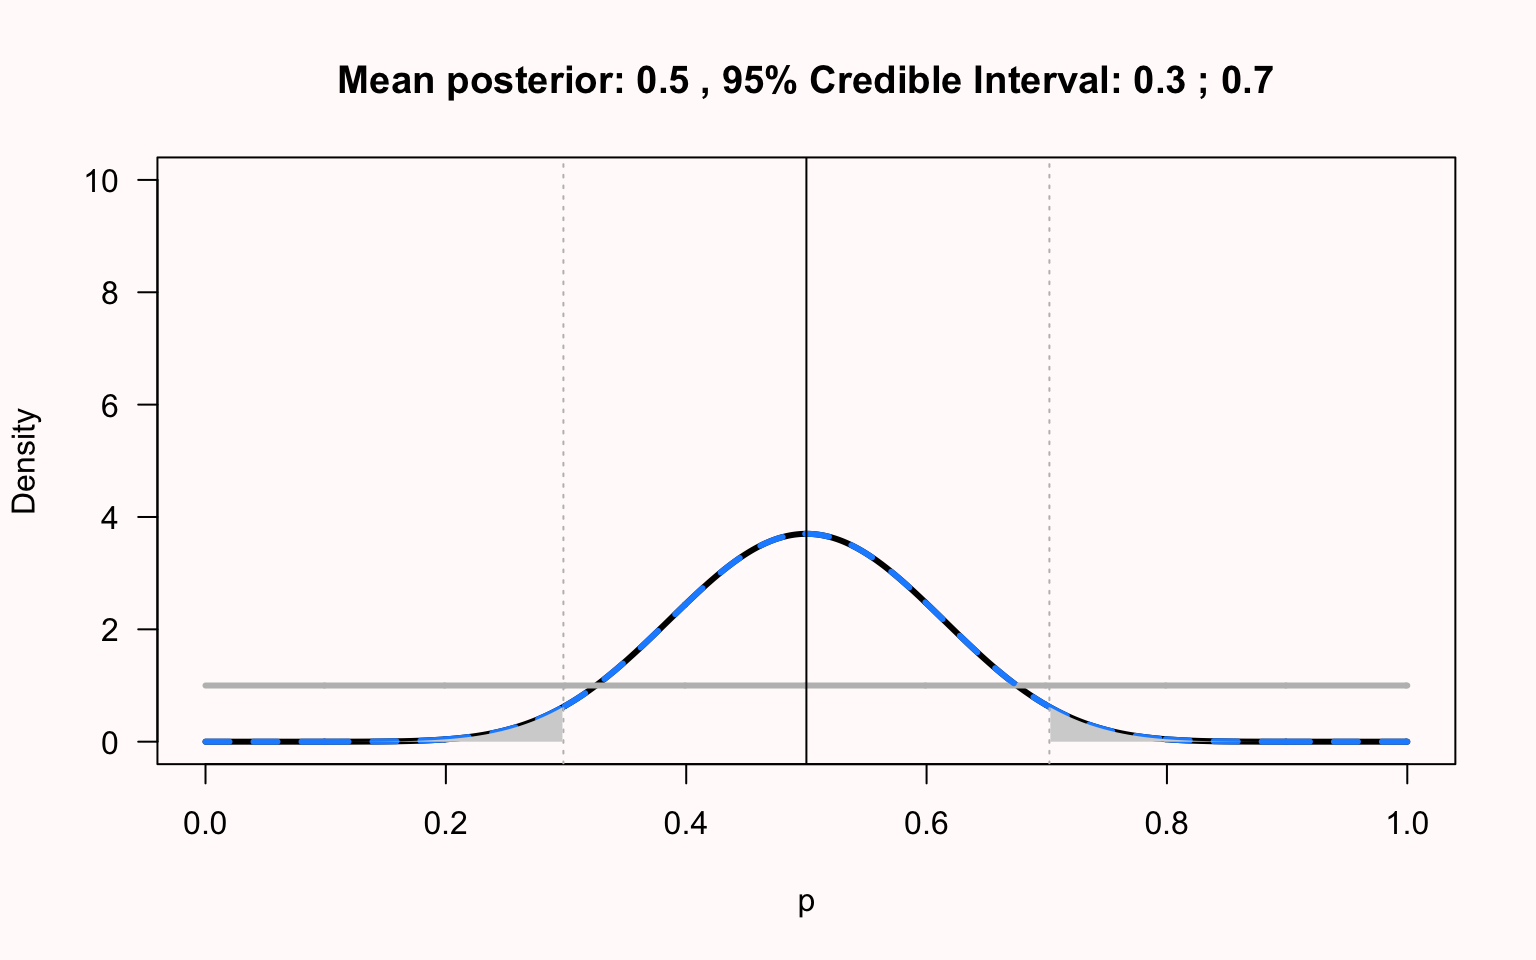
\includegraphics[width=1\linewidth]{04-bayes_files/figure-latex/bayes4-1} 

}

\caption{Plot for the prior, likelihood, and posterior.}\label{fig:bayes4}
\end{figure}

The Bayes Factor is used to quantify this increase in relative evidence. Let's calculate the Bayes Factor for the hypothesis that the coin is fair for the newborn. The Bayes Factor is simply the value of the posterior distribution at \emph{p} = 0.5, divided by the value of the prior distribution at \emph{p} = 0.5:

BF10 = Beta(\emph{p} = 0.5, 11, 11)/Beta(\emph{p} = 0.5, 1, 1) = 3.70/1 = 3.70

You can check this in an \href{http://pcl.missouri.edu/bf-binomial}{online Bayes Factor calculator} \citep{rouder_bayesian_2009}. At successes, fill in 10, at trials, fill in 20. We want to calculate the Bayes Factor for the point null value of \emph{p} = 0.5, so fill in 0.5. The \(\alpha\) and \(\beta\) for the prior are both 1, given the newborns prior of Beta(1,1). Clicking `submit query' will give you the Bayes factor of 3.70.



\begin{figure}

{\centering 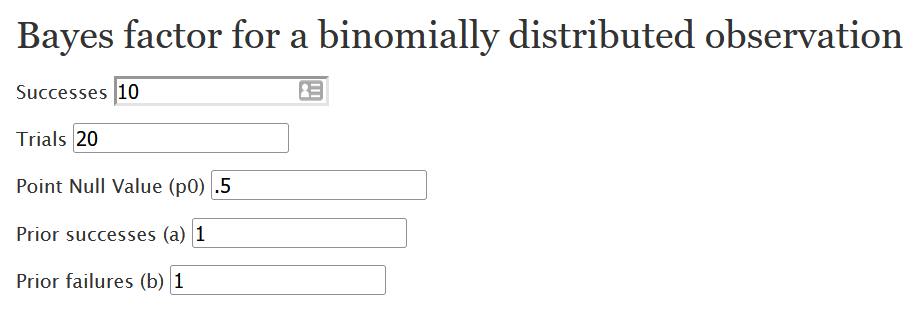
\includegraphics[width=1\linewidth]{images/binombayesonline} 

}

\caption{Screenshot of the online calculator for binomially distributed observations.}\label{fig:gpower-screenshot-bayes}
\end{figure}

We can calculate and plot the Bayes Factor, and show the prior (grey), likelihood (dashed blue) and posterior (black). For the example of 20 flips, 10 heads, and the newborn prior, the plot looks like this:



\begin{figure}

{\centering 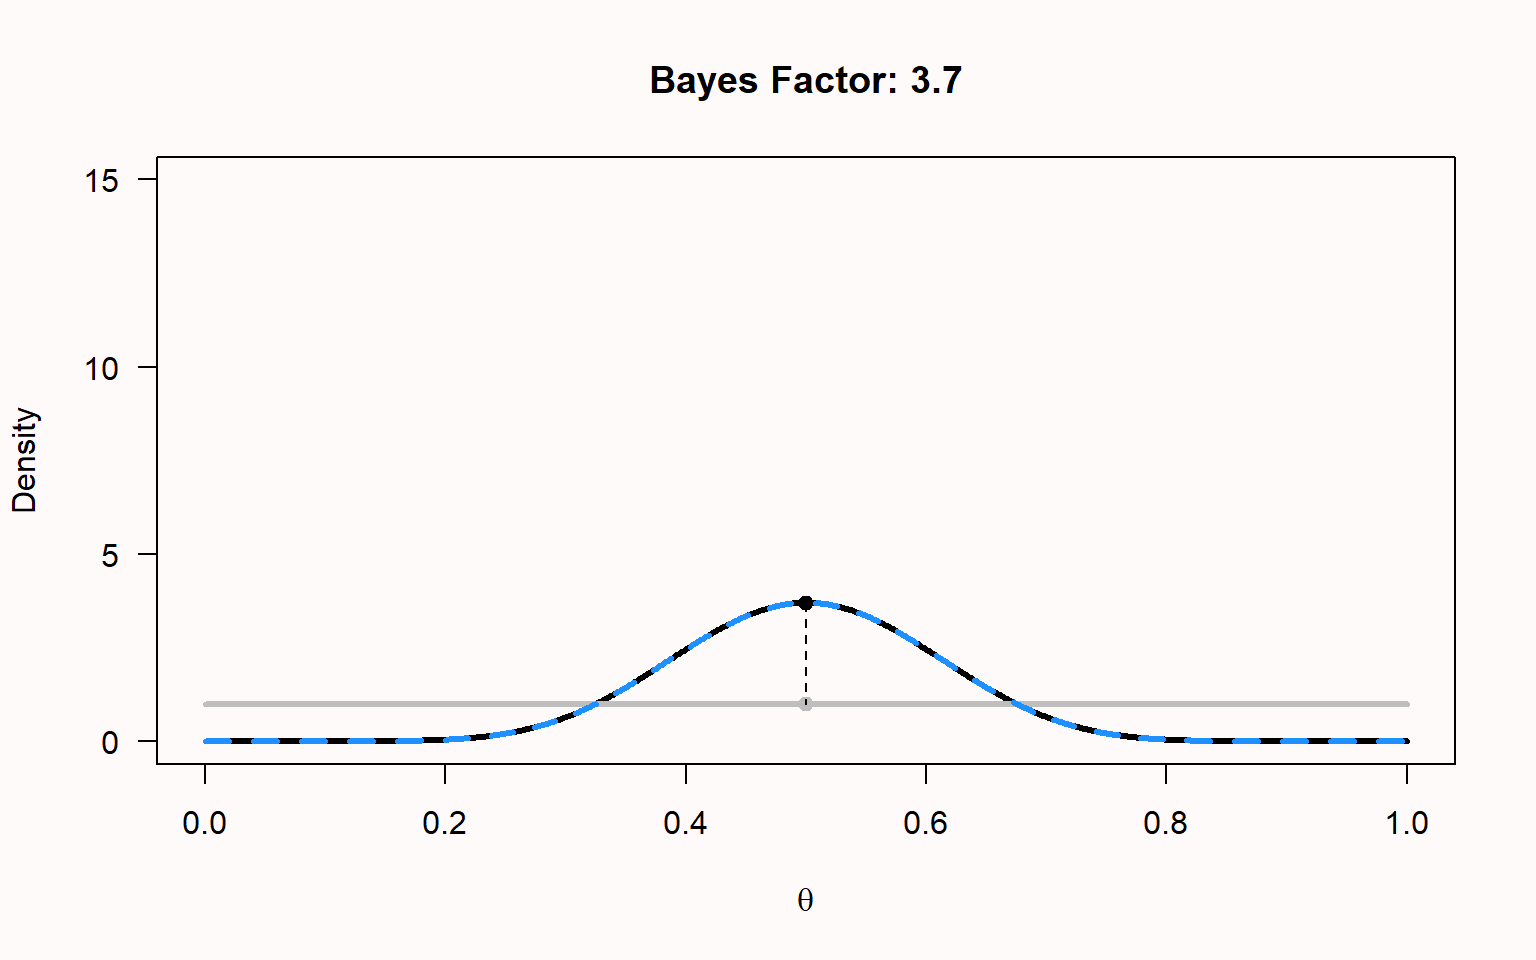
\includegraphics[width=1\linewidth]{04-bayes_files/figure-latex/bayes6-1} 

}

\caption{Plot for the prior, likelihood, and posterior.}\label{fig:bayes6}
\end{figure}

We see that for the newborn, \emph{p} = 0.5 has become more probable, but so has \emph{p} = 0.4. Now let's assume the strong skeptic, who believes the coin is fair with a prior of Beta(100, 100), buys the coin and flips it 100 times. Surprisingly, the coin comes up heads 90 out of 100 flips. The plot of the prior, likelihood, and posterior now looks much more extreme, because we had a very informed prior, and extremely different data. We see the grey prior distribution, the dashed blue likelihood based on the data, and the posterior distribution in black. The Bayes Factor of 0 (note that the value is rounded, and is extremely small, but not exactly zero) - represents the substantial drop in belief that the coin is fair -- indeed, this now seems an untenable hypothesis, even for the strong skeptic. It shows how data can update your belief. Where a newborn would now completely believe that the true \emph{p} for the coin is somewhere around 0.9, the strong skeptic has more reason to believe the \emph{p} is around 0.65, due to the strong prior conviction that the coin is fair. Given enough data, even this strong skeptic will become convinced that the coin will return heads most of the time as well.



\begin{figure}

{\centering 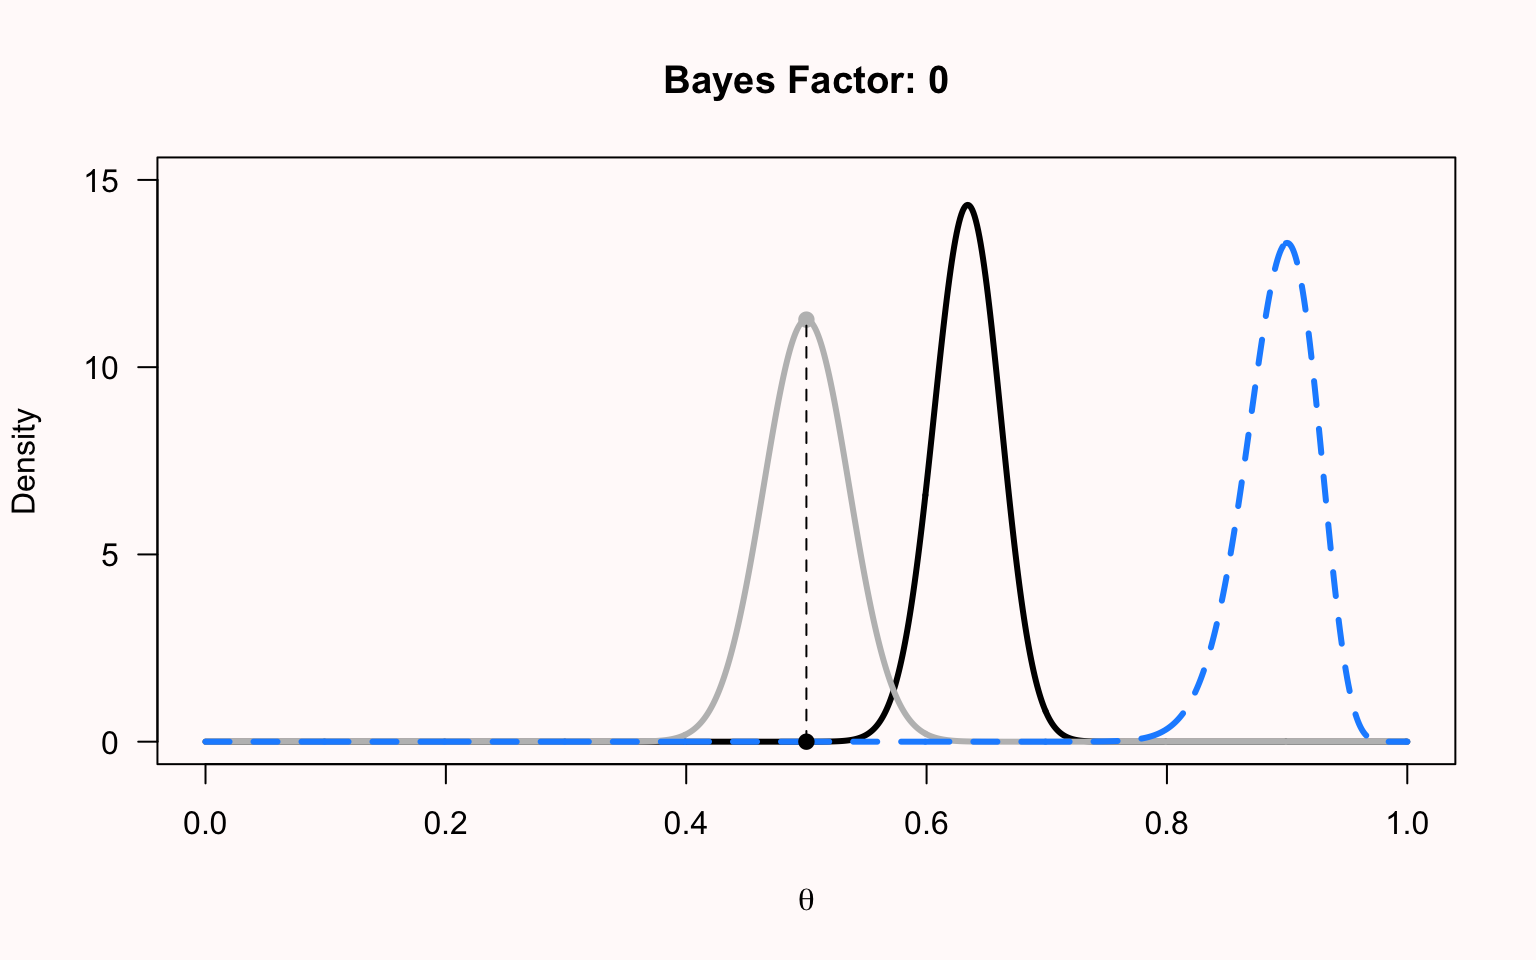
\includegraphics[width=1\linewidth]{04-bayes_files/figure-latex/bayes7-1} 

}

\caption{Plot for the prior, likelihood, and posterior.}\label{fig:bayes7}
\end{figure}

We can now also see the difference between a likelihood inference approach, and a Bayesian inference approach. In likelihood inference, you can compare different values of \emph{p} for the same likelihood curve (e.g., \emph{p} = 0.5 vs \emph{p} = 0.8) and calculate the likelihood ratio. In Bayesian inference, you can compare the difference between the prior and the posterior for the same value of \emph{p}, and calculate the Bayes Factor.

If you have never seen Bayes Factors before, you might find it difficult to interpret the numbers. As with any guideline (e.g., interpreting effect sizes as small, medium, and large) there is criticism on the use of benchmarks. On the other hand, you have to start somewhere in getting a feel for what Bayes Factors mean. A Bayes factor between 1 and 3 is considered `not worth more than a bare mention', larger than 3 (or smaller than 1/3) is considered `substantial', and larger than 10 (or smaller than 1/10) is considered `strong' \citep{jeffreys_theory_1939}. These labels refer to the increase in how much you believe a specific hypothesis, not in the posterior belief in that hypothesis. If you think extra-sensory perception is extremely implausible, a single study with a BF = 14 will increase your belief, but you will now think extra-sensory perception is pretty much extremely implausible.

Bayes factors are often promoted as an alternative to \emph{p}-values. One stated benefit is that they can provide support both for the alternative, as for the null \citep{dienes_using_2014}. However, the same can be achieved with frequentist equivalence tests, as we will see in the chapter on \protect\hyperlink{equivalencetest}{equivalence testing}, and inferences based on Bayes factors and equivalence tests typically lead to the same conclusions \citep{lakens_improving_2020}. Another reason that some people give to switch to Bayes factors instead of \emph{p}-values is that, as we saw in the chapter on \protect\hyperlink{misconceptions}{\emph{p}-values}, \emph{p}-values are often misunderstood. However, not surprisingly, Bayes factors are at least as often misunderstood and misused \citep{wong_potential_2021}. Statistical inferences are hard, and thinking about probabilities is not something we get right by trusting our intuition. We need to train ourselves to draw correct inferences, and switching to a different statistic will not prevent misuse.

\hypertarget{bayesest}{%
\section{Bayesian Estimation}\label{bayesest}}

The posterior distribution summarizes our belief about the expected number of heads when flipping a coin after seeing the data, by averaging over our prior beliefs and the data (or the likelihood). The mean of a Beta distribution can be calculated by \(\alpha\)/(\(\alpha\)+\(\beta\)). We can thus easily calculate the mean of a posterior distribution, which is the expected value based on our prior beliefs and the data.

We can also calculate a \textbf{credible interval} around the mean, which is a Bayesian version of a confidence interval with a slightly different interpretation. Instead of the Frequentist interpretation where a parameter has one (unknown) true value, the Bayesian approach considers the data fixed, but allow the parameter to vary. In Bayesian approaches, probability distributions represent our degree of belief. When calculating a credible interval, one is saying `I believe it is 95\% probable (given my prior and the data) that the true parameter falls within this credible interval'. A 95\% credible interval is simply the area of the posterior distribution between the 0.025 and 0.975 quantiles.

A credible interval and a confidence interval are the same, when a uniform prior (e.g., Beta(1,1)) is used. In this case, credible interval is numerically identical to the confidence interval. Only the interpretation differs. Whenever an informed prior is used, the credible interval and confidence interval differ. If the chosen prior is not representative of the truth, the credible interval will not be representative of the truth, but it is always a correct formalization of your beliefs. For a single confidence interval, the probability that it contains the true population parameter is either 0 or 1. Only in the long run will 95\% of confidence intervals contain the true population parameter. These are important differences between Bayesian credible intervals and Frequentist confidence intervals to keep in mind.

We can plot the mean for the posterior when 10 heads out of 20 coin flips are observed, given a uniform prior.



\begin{figure}

{\centering 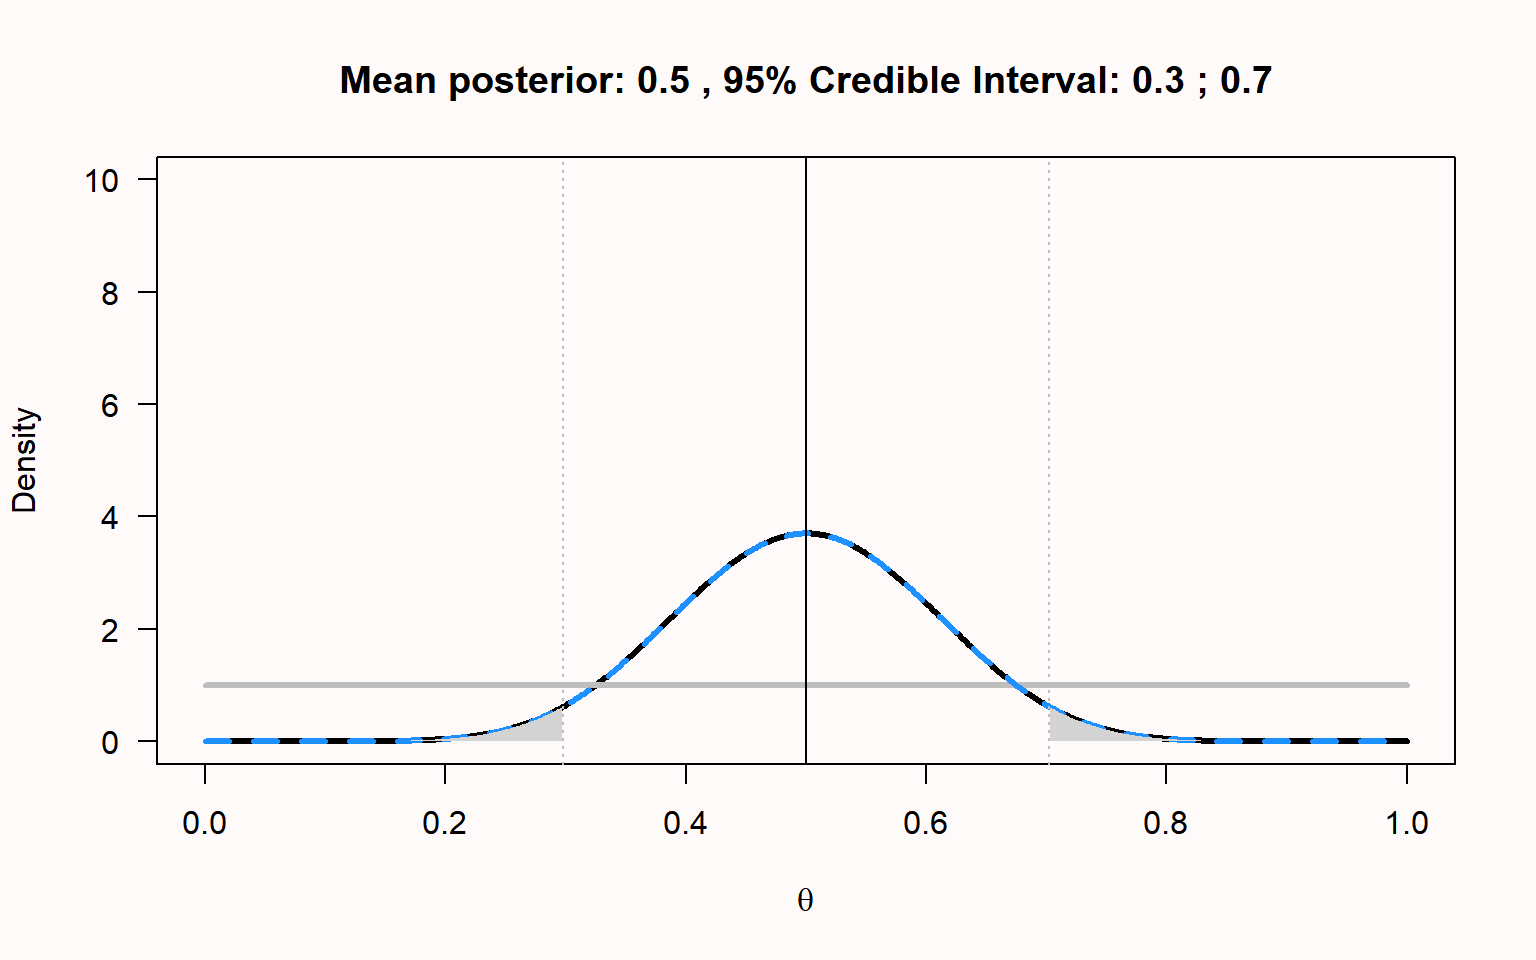
\includegraphics[width=1\linewidth]{04-bayes_files/figure-latex/bayes8-1} 

}

\caption{Plot for the mean of the posterior when 10 out of 20 heads are observed given a uniform prior.}\label{fig:bayes8}
\end{figure}

We can also use the `binom' package to calculate the posterior mean, credible interval, and \textbf{highest density interval (HDI)}. The highest density interval is an alternative to the credible interval that works better when the posterior beta distribution is skewed (and is identical when the posterior distribution is symmetrical. We won't go into the calculations of the HDI here.

\begin{Shaded}
\begin{Highlighting}[]
\FunctionTok{library}\NormalTok{(binom)}

\NormalTok{n }\OtherTok{\textless{}{-}} \DecValTok{20} \CommentTok{\# set total trials}
\NormalTok{x }\OtherTok{\textless{}{-}} \DecValTok{10} \CommentTok{\# set successes}
\NormalTok{aprior }\OtherTok{\textless{}{-}} \DecValTok{1} \CommentTok{\# Set the alpha for the Beta distribution for the prior}
\NormalTok{bprior }\OtherTok{\textless{}{-}} \DecValTok{1} \CommentTok{\# Set the beta for the Beta distribution for the prior}

\FunctionTok{binom.bayes}\NormalTok{(x, n, }\AttributeTok{type =} \StringTok{"central"}\NormalTok{, }\AttributeTok{prior.shape1 =}\NormalTok{ aprior, }\AttributeTok{prior.shape2 =}\NormalTok{ bprior)}
\end{Highlighting}
\end{Shaded}

\begin{verbatim}
##   method  x  n shape1 shape2 mean     lower     upper  sig
## 1  bayes 10 20     11     11  0.5 0.2978068 0.7021932 0.05
\end{verbatim}

\begin{Shaded}
\begin{Highlighting}[]
\FunctionTok{binom.bayes}\NormalTok{(x, n, }\AttributeTok{type =} \StringTok{"highest"}\NormalTok{, }\AttributeTok{prior.shape1 =}\NormalTok{ aprior, }\AttributeTok{prior.shape2 =}\NormalTok{ bprior)}
\end{Highlighting}
\end{Shaded}

\begin{verbatim}
##   method  x  n shape1 shape2 mean     lower     upper  sig
## 1  bayes 10 20     11     11  0.5 0.2978068 0.7021932 0.05
\end{verbatim}

The posterior mean is identical to the Frequentist mean, but this is only the case when the mean of the prior equals the mean of the likelihood \citep{albers_credible_2018}. In your research, you will most likely need other calculations than the binomial example we have used here, and a lot of Bayesian tests are now available in the free open source software package \href{https://jasp-stats.org/}{JASP}. The math and the priors become more complex, but the basic idea remains the same. You can use Bayesian statistics to quantify relative evidence, which can inform you how much we should believe, or update our beliefs, in theories.

This chapter showed the essence of Bayesian inference, where we decide upon a prior distribution, collect data and calculate a marginal likelihood, and use these to calculate a posterior distribution. From this posterior distribution, we can estimate the mean and the 95\% credible interval. For any specific hypothesis, we can calculate the relative evidence for a posterior model, compared to a prior model, through the Bayes Factor. There are many different flavors of Bayesian statistics. This means there are disagreements among Bayesians about what the best approach to statistical inferences is, which are at least as vehement as the disagreements between frequentists and Bayesians. For example, many Bayesians dislike Bayes factors \citep{mcelreath_statistical_2016}. Some Bayesians dislike subjective priors as used in \textbf{subjective Bayesian analysis}, and instead prefer what is known as \textbf{objective Bayesian analysis} \citep{berger_interplay_2004}. Teaching material on Bayesian statistics will often present it as superior to frequentist statistics. For a more balanced educational lecture on Bayesian vs.~frequentist statistics that more honestly highlights the strengths and weaknesses of both approach, see the first 50 minutes of \href{https://www.youtube.com/watch?v=HUAE26lNDuE}{this lecture by Michael I. Jordan}.

\hypertarget{test-yourself-3}{%
\section{Test Yourself}\label{test-yourself-3}}

\textbf{Q1}: The true believer had a prior of Beta(1,0.5). After observing 10 heads out of 20 coin flips, what is the posterior distribution, given that α* = α + x and β* = β + n -- x?

\begin{enumerate}
\def\labelenumi{\Alph{enumi})}
\tightlist
\item
  Beta(10, 10)
\item
  Beta(11, 10.5)
\item
  Beta(10, 20)
\item
  Beta(11, 20.5)
\end{enumerate}

\textbf{Q2}: The strong skeptic had a prior of Beta(100,100). After observing 50 heads out of 100 coin flips, what is the posterior distribution, given that α* = α + x and β* = β + n -- x?

\begin{enumerate}
\def\labelenumi{\Alph{enumi})}
\tightlist
\item
  Beta(50, 50)
\item
  Beta(51, 51)
\item
  Beta(150, 150)
\item
  Beta(151, 151)
\end{enumerate}

Copy the R script below into R. This script requires 5 input parameters (identical to the Bayes Factor calculator website used above). These are the hypothesis you want to examine (e.g., when evaluating whether a coin is fair, \emph{p} = 0.5), the total number of trials (e.g., 20 flips), the number of successes (e.g., 10 heads), and the \(\alpha\) and \(\beta\) values for the Beta distribution for the prior (e.g., \(\alpha\) = 1 and \(\beta\) = 1 for a uniform prior). Run the script. It will calculate the Bayes Factor, and plot the prior (grey), likelihood (dashed blue) and posterior (black).

\begin{Shaded}
\begin{Highlighting}[]
\NormalTok{H0 }\OtherTok{\textless{}{-}} \FloatTok{0.5} \CommentTok{\# Set the point null hypothesis you want to calculate the Bayes Factor for}
\NormalTok{n }\OtherTok{\textless{}{-}} \DecValTok{20} \CommentTok{\# set total trials}
\NormalTok{x }\OtherTok{\textless{}{-}} \DecValTok{10} \CommentTok{\# set successes}
\NormalTok{aprior }\OtherTok{\textless{}{-}} \DecValTok{1} \CommentTok{\# Set the alpha for the Beta distribution for the prior}
\NormalTok{bprior }\OtherTok{\textless{}{-}} \DecValTok{1} \CommentTok{\# Set the beta for the Beta distribution for the prior}

\NormalTok{alikelihood }\OtherTok{\textless{}{-}}\NormalTok{ x }\SpecialCharTok{+} \DecValTok{1} \CommentTok{\# Calculate the alpha for the Beta distribution for the likelihood}
\NormalTok{blikelihood }\OtherTok{\textless{}{-}}\NormalTok{ n }\SpecialCharTok{{-}}\NormalTok{ x }\SpecialCharTok{+} \DecValTok{1} \CommentTok{\# Calculate the beta for the Beta distribution for the likelihood}
\NormalTok{aposterior }\OtherTok{\textless{}{-}}\NormalTok{ aprior }\SpecialCharTok{+}\NormalTok{ alikelihood }\SpecialCharTok{{-}} \DecValTok{1} \CommentTok{\# Calculate the alpha for the Beta distribution for the posterior}
\NormalTok{bposterior }\OtherTok{\textless{}{-}}\NormalTok{ bprior }\SpecialCharTok{+}\NormalTok{ blikelihood }\SpecialCharTok{{-}} \DecValTok{1} \CommentTok{\# Calculate the beta for the Beta distribution for the posterior}

\NormalTok{theta }\OtherTok{\textless{}{-}} \FunctionTok{seq}\NormalTok{(}\DecValTok{0}\NormalTok{, }\DecValTok{1}\NormalTok{, }\FloatTok{0.001}\NormalTok{) }\CommentTok{\# create probability range p from 0 to 1}
\NormalTok{prior }\OtherTok{\textless{}{-}} \FunctionTok{dbeta}\NormalTok{(theta, aprior, bprior)}
\NormalTok{likelihood }\OtherTok{\textless{}{-}} \FunctionTok{dbeta}\NormalTok{(theta, alikelihood, blikelihood)}
\NormalTok{posterior }\OtherTok{\textless{}{-}} \FunctionTok{dbeta}\NormalTok{(theta, aposterior, bposterior)}

\CommentTok{\# Create plot}
\FunctionTok{plot}\NormalTok{(theta, posterior, }\AttributeTok{ylim =} \FunctionTok{c}\NormalTok{(}\DecValTok{0}\NormalTok{, }\DecValTok{15}\NormalTok{), }\AttributeTok{type =} \StringTok{"l"}\NormalTok{, }\AttributeTok{lwd =} \DecValTok{3}\NormalTok{, }\AttributeTok{xlab =} \StringTok{"p"}\NormalTok{, }\AttributeTok{ylab =} \StringTok{"Density"}\NormalTok{, }\AttributeTok{las =} \DecValTok{1}\NormalTok{)}
\FunctionTok{lines}\NormalTok{(theta, prior, }\AttributeTok{col =} \StringTok{"grey"}\NormalTok{, }\AttributeTok{lwd =} \DecValTok{3}\NormalTok{)}
\FunctionTok{lines}\NormalTok{(theta, likelihood, }\AttributeTok{lty =} \DecValTok{2}\NormalTok{, }\AttributeTok{lwd =} \DecValTok{3}\NormalTok{, }\AttributeTok{col =} \StringTok{"dodgerblue"}\NormalTok{)}
\NormalTok{BF10 }\OtherTok{\textless{}{-}} \FunctionTok{dbeta}\NormalTok{(H0, aposterior, bposterior) }\SpecialCharTok{/} \FunctionTok{dbeta}\NormalTok{(H0, aprior, bprior)}
\FunctionTok{points}\NormalTok{(H0, }\FunctionTok{dbeta}\NormalTok{(H0, aposterior, bposterior), }\AttributeTok{pch =} \DecValTok{19}\NormalTok{)}
\FunctionTok{points}\NormalTok{(H0, }\FunctionTok{dbeta}\NormalTok{(H0, aprior, bprior), }\AttributeTok{pch =} \DecValTok{19}\NormalTok{, }\AttributeTok{col =} \StringTok{"grey"}\NormalTok{)}
\FunctionTok{segments}\NormalTok{(H0, }\FunctionTok{dbeta}\NormalTok{(H0, aposterior, bposterior), H0, }\FunctionTok{dbeta}\NormalTok{(H0, aprior, bprior), }\AttributeTok{lty =} \DecValTok{2}\NormalTok{)}
\FunctionTok{title}\NormalTok{(}\FunctionTok{paste}\NormalTok{(}\StringTok{"Bayes Factor:"}\NormalTok{, }\FunctionTok{round}\NormalTok{(BF10, }\AttributeTok{digits =} \DecValTok{2}\NormalTok{)))}
\end{Highlighting}
\end{Shaded}

\begin{center}\includegraphics[width=1\linewidth]{04-bayes_files/figure-latex/unnamed-chunk-3-1} \end{center}

We see that for the newborn, \emph{p} = 0.5 has become more probable, but so has \emph{p} = 0.4.

\textbf{Q3}: Change the hypothesis in the first line from 0.5 to 0.675, and run the script. If you were testing the idea that this coin returns 67.5\% heads, which statement is true?

\begin{enumerate}
\def\labelenumi{\Alph{enumi})}
\tightlist
\item
  Your belief in this hypothesis, given the data, would have decreased.
\item
  Your belief in this hypothesis, given the data, would have stayed the same.
\item
  Your belief in this hypothesis, given the data, would have increased.
\end{enumerate}

\textbf{Q4}: Change the hypothesis in the first line back to 0.5. Let's look at the increase in the belief of the hypothesis \emph{p} = 0.5 for the strong skeptic after 10 heads out of 20 coin flips. Change the \(\alpha\) for the prior in line 4 to 100 and the \(\beta\) for the prior in line 5 to 100. Run the script. Compare the Figure from R to the increase in belief for the newborn (in the plot on the previous page). Which statement is true?

\begin{enumerate}
\def\labelenumi{\Alph{enumi})}
\tightlist
\item
  The belief in the hypothesis that \emph{p} = 0.5, given the data, has \textbf{increased} for the strong skeptic, but \textbf{not} as much as it has for the newborn.
\item
  The belief in the hypothesis that \emph{p} = 0.5, given the data, has \textbf{increased} for the strong skeptic, \textbf{exactly as much} as it has for the newborn.
\item
  The belief in the hypothesis that \emph{p} = 0.5, given the data, has \textbf{increased} for the strong skeptic, and \textbf{much more} than it has for the newborn.
\item
  The belief in the hypothesis that \emph{p} = 0.5, given the data, has \textbf{decreased} for the strong skeptic.
\end{enumerate}

Copy the R script below and run it. The script will plot the mean for the posterior when 10 heads out of 20 coin flips are observed, given a uniform prior (as in \ref{fig:bayes8}) . The script will also use the `binom' package to calculate the posterior mean, credible interval, and \textbf{highest density interval (HDI)}. The highest density interval is an alternative to the credible interval that works better when the posterior beta distribution is skewed (and is identical when the posterior distribution is symmetrical. We won't go into the calculations of the HDI here.

\begin{Shaded}
\begin{Highlighting}[]
\NormalTok{n }\OtherTok{\textless{}{-}} \DecValTok{20} \CommentTok{\# set total trials}
\NormalTok{x }\OtherTok{\textless{}{-}} \DecValTok{10} \CommentTok{\# set successes}
\NormalTok{aprior }\OtherTok{\textless{}{-}} \DecValTok{1} \CommentTok{\# Set the alpha for the Beta distribution for the prior}
\NormalTok{bprior }\OtherTok{\textless{}{-}} \DecValTok{1} \CommentTok{\# Set the beta for the Beta distribution for the prior}

\NormalTok{ymax }\OtherTok{\textless{}{-}} \DecValTok{10} \CommentTok{\# set max y{-}axis}

\NormalTok{alikelihood }\OtherTok{\textless{}{-}}\NormalTok{ x }\SpecialCharTok{+} \DecValTok{1} \CommentTok{\# Calculate the alpha for the Beta distribution for the likelihood}
\NormalTok{blikelihood }\OtherTok{\textless{}{-}}\NormalTok{ n }\SpecialCharTok{{-}}\NormalTok{ x }\SpecialCharTok{+} \DecValTok{1} \CommentTok{\# Calculate the beta for the Beta distribution for the likelihood}
\NormalTok{aposterior }\OtherTok{\textless{}{-}}\NormalTok{ aprior }\SpecialCharTok{+}\NormalTok{ alikelihood }\SpecialCharTok{{-}} \DecValTok{1} \CommentTok{\# Calculate the alpha for the Beta distribution for the posterior}
\NormalTok{bposterior }\OtherTok{\textless{}{-}}\NormalTok{ bprior }\SpecialCharTok{+}\NormalTok{ blikelihood }\SpecialCharTok{{-}} \DecValTok{1} \CommentTok{\# Calculate the beta for the Beta distribution for the posterior}

\NormalTok{theta }\OtherTok{\textless{}{-}} \FunctionTok{seq}\NormalTok{(}\DecValTok{0}\NormalTok{, }\DecValTok{1}\NormalTok{, }\FloatTok{0.001}\NormalTok{) }\CommentTok{\# create probability range p from 0 to 1}
\NormalTok{prior }\OtherTok{\textless{}{-}} \FunctionTok{dbeta}\NormalTok{(theta, aprior, bprior) }\CommentTok{\# deterine prior distribution}
\NormalTok{likelihood }\OtherTok{\textless{}{-}} \FunctionTok{dbeta}\NormalTok{(theta, alikelihood, blikelihood) }\CommentTok{\# determine likelihood distribution}
\NormalTok{posterior }\OtherTok{\textless{}{-}} \FunctionTok{dbeta}\NormalTok{(theta, aposterior, bposterior) }\CommentTok{\# determine posterior distribution}
\FunctionTok{plot}\NormalTok{(theta, posterior, }\AttributeTok{ylim =} \FunctionTok{c}\NormalTok{(}\DecValTok{0}\NormalTok{, ymax), }\AttributeTok{type =} \StringTok{"l"}\NormalTok{, }\AttributeTok{lwd =} \DecValTok{3}\NormalTok{, }\AttributeTok{xlab =} \FunctionTok{bquote}\NormalTok{(theta), }\AttributeTok{ylab =} \StringTok{"Density"}\NormalTok{, }\AttributeTok{las =} \DecValTok{1}\NormalTok{) }\CommentTok{\# draw posterior distribution}
\FunctionTok{lines}\NormalTok{(theta, prior, }\AttributeTok{col =} \StringTok{"grey"}\NormalTok{, }\AttributeTok{lwd =} \DecValTok{3}\NormalTok{) }\CommentTok{\# draw prior distribution}
\FunctionTok{lines}\NormalTok{(theta, likelihood, }\AttributeTok{lty =} \DecValTok{2}\NormalTok{, }\AttributeTok{lwd =} \DecValTok{3}\NormalTok{, }\AttributeTok{col =} \StringTok{"dodgerblue"}\NormalTok{) }\CommentTok{\# draw likelihood distribution}
\NormalTok{LL }\OtherTok{\textless{}{-}} \FunctionTok{qbeta}\NormalTok{(.}\DecValTok{025}\NormalTok{, aposterior, bposterior) }\CommentTok{\# calculate lower limit credible interval}
\NormalTok{UL }\OtherTok{\textless{}{-}} \FunctionTok{qbeta}\NormalTok{(.}\DecValTok{975}\NormalTok{, aposterior, bposterior) }\CommentTok{\# calculate upper limit credible interval}
\FunctionTok{abline}\NormalTok{(}\AttributeTok{v =}\NormalTok{ aposterior }\SpecialCharTok{/}\NormalTok{ (aposterior }\SpecialCharTok{+}\NormalTok{ bposterior)) }\CommentTok{\# draw line mean}
\FunctionTok{abline}\NormalTok{(}\AttributeTok{v =}\NormalTok{ LL, }\AttributeTok{col =} \StringTok{"grey"}\NormalTok{, }\AttributeTok{lty =} \DecValTok{3}\NormalTok{) }\CommentTok{\# draw line lower limit}
\FunctionTok{abline}\NormalTok{(}\AttributeTok{v =}\NormalTok{ UL, }\AttributeTok{col =} \StringTok{"grey"}\NormalTok{, }\AttributeTok{lty =} \DecValTok{3}\NormalTok{) }\CommentTok{\# draw line upper limit}
\FunctionTok{polygon}\NormalTok{(}\FunctionTok{c}\NormalTok{(theta[theta }\SpecialCharTok{\textless{}}\NormalTok{ LL], }\FunctionTok{rev}\NormalTok{(theta[theta }\SpecialCharTok{\textless{}}\NormalTok{ LL])), }\FunctionTok{c}\NormalTok{(posterior[theta }\SpecialCharTok{\textless{}}\NormalTok{ LL], }\FunctionTok{rep}\NormalTok{(}\DecValTok{0}\NormalTok{, }\FunctionTok{sum}\NormalTok{(theta }\SpecialCharTok{\textless{}}\NormalTok{ LL))), }\AttributeTok{col =} \StringTok{"lightgrey"}\NormalTok{, }\AttributeTok{border =} \ConstantTok{NA}\NormalTok{)}
\FunctionTok{polygon}\NormalTok{(}\FunctionTok{c}\NormalTok{(theta[theta }\SpecialCharTok{\textgreater{}}\NormalTok{ UL], }\FunctionTok{rev}\NormalTok{(theta[theta }\SpecialCharTok{\textgreater{}}\NormalTok{ UL])), }\FunctionTok{c}\NormalTok{(posterior[theta }\SpecialCharTok{\textgreater{}}\NormalTok{ UL], }\FunctionTok{rep}\NormalTok{(}\DecValTok{0}\NormalTok{, }\FunctionTok{sum}\NormalTok{(theta }\SpecialCharTok{\textgreater{}}\NormalTok{ UL))), }\AttributeTok{col =} \StringTok{"lightgrey"}\NormalTok{, }\AttributeTok{border =} \ConstantTok{NA}\NormalTok{)}
\FunctionTok{title}\NormalTok{(}\FunctionTok{paste}\NormalTok{(}\StringTok{"Mean posterior:"}\NormalTok{, }\FunctionTok{round}\NormalTok{((aposterior }\SpecialCharTok{/}\NormalTok{ (aposterior }\SpecialCharTok{+}\NormalTok{ bposterior)), }\AttributeTok{digits =} \DecValTok{5}\NormalTok{), }\StringTok{", 95\% Credible Interval:"}\NormalTok{, }\FunctionTok{round}\NormalTok{(LL, }\AttributeTok{digits =} \DecValTok{2}\NormalTok{), }\StringTok{";"}\NormalTok{, }\FunctionTok{round}\NormalTok{(UL, }\AttributeTok{digits =} \DecValTok{2}\NormalTok{)))}
\end{Highlighting}
\end{Shaded}

\begin{center}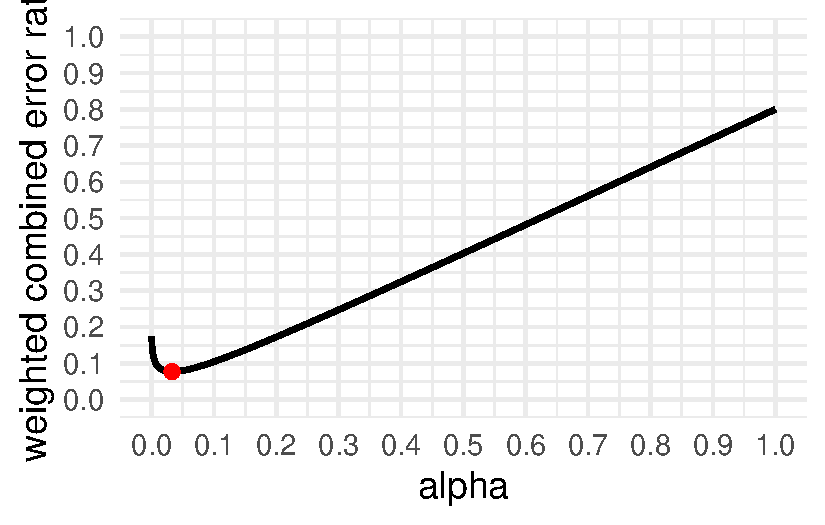
\includegraphics[width=1\linewidth]{04-bayes_files/figure-latex/unnamed-chunk-4-1} \end{center}

\begin{Shaded}
\begin{Highlighting}[]
\ControlFlowTok{if}\NormalTok{ (}\SpecialCharTok{!}\FunctionTok{require}\NormalTok{(binom)) \{}
  \FunctionTok{install.packages}\NormalTok{(}\StringTok{"binom"}\NormalTok{)}
\NormalTok{\}}
\FunctionTok{library}\NormalTok{(binom)}
\FunctionTok{binom.bayes}\NormalTok{(x, n, }\AttributeTok{type =} \StringTok{"central"}\NormalTok{, }\AttributeTok{prior.shape1 =}\NormalTok{ aprior, }\AttributeTok{prior.shape2 =}\NormalTok{ bprior)}
\end{Highlighting}
\end{Shaded}

\begin{verbatim}
##   method  x  n shape1 shape2 mean     lower     upper  sig
## 1  bayes 10 20     11     11  0.5 0.2978068 0.7021932 0.05
\end{verbatim}

\begin{Shaded}
\begin{Highlighting}[]
\FunctionTok{binom.bayes}\NormalTok{(x, n, }\AttributeTok{type =} \StringTok{"highest"}\NormalTok{, }\AttributeTok{prior.shape1 =}\NormalTok{ aprior, }\AttributeTok{prior.shape2 =}\NormalTok{ bprior)}
\end{Highlighting}
\end{Shaded}

\begin{verbatim}
##   method  x  n shape1 shape2 mean     lower     upper  sig
## 1  bayes 10 20     11     11  0.5 0.2978068 0.7021932 0.05
\end{verbatim}

The posterior mean is identical to the Frequentist mean, but this is only the case when the mean of the prior equals the mean of the likelihood.

\textbf{Q5}: Assume the outcome of 20 coin flips had been 18 heads. Change x to 18 in line 2 and run the script. Remember that the mean of the prior Beta(1,1) distribution is α/(α+β), or 1/(1+1) = 0.5. The Frequentist mean is simply x/n, or 18/20=0.9. Which statement is true?

\begin{enumerate}
\def\labelenumi{\Alph{enumi})}
\tightlist
\item
  The frequentist mean is \textbf{higher} than the mean of the posterior, because by combining the prior with the data, the mean of the posterior is \textbf{closer} to the mean of the prior distribution.
\item
  The frequentist mean is \textbf{lower} than the mean of the posterior, because by combining the prior with the data, the mean of the posterior is \textbf{closer} to the mean of the prior distribution.
\item
  The frequentist mean is \textbf{higher} than the mean of the posterior, because by combining the prior with the data, the mean of the posterior is \textbf{further from} to the mean of the prior distribution.
\item
  The frequentist mean is \textbf{lower} than the mean of the posterior, because by combining the prior with the data, the mean of the posterior is \textbf{further from} to the mean of the prior distribution.
\end{enumerate}

\textbf{Q6}: What is, today, your best estimate of the probability that the sun rises every day? Assume you were born with an uniform Beta(1,1) prior. The sun can either rise, or it does not. Assume you have seen the sun every day since you were born, which means there has been a continuous string of successes for every day you have been alive. It is ok to estimate the days you have been alive by just multiplying your age by 365 days. What is your best estimate of the probability that the sun will rise?

\textbf{Q7}: What would have been the best estimate from a Frequentist perspective?

\textbf{Q8}: What do you think the goal of science is? Rozeboom \citeyearpar{rozeboom_fallacy_1960} has criticized Neyman-Pearson hypothesis testing by stating:

\begin{quote}
But the primary aim of a scientific experiment is not to precipitate decisions, but to make an appropriate adjustment in the degree to which one accepts, or believes, the hypothesis or hypotheses being tested''.
\end{quote}

Frick \citeyearpar{frick_appropriate_1996} has argued against Rozeboom, by stating:

\begin{quote}
Rozeboom (1960) suggested that scientists should not be making decisions about claims, they should be calculating and updating the probability of these claims. However, this does not seem practical. If there were only a handful of potential claims in any given area of psychology, it would be feasible to assign them probabilities, to be constantly updating the probabilities, and to expect experimenters to keep track of these ever-changing probabilities. In fact, just the number of claims in psychology is overwhelming. It would probably be impossible for human beings to keep track of the probability for each claim, especially if these probabilities were constantly changing. In any case, scientists do not assign probabilities to claims. Instead, scientists act like the goal of science is to collect a corpus of claims that are considered to be established (Giere, 1972).
\end{quote}

When it comes to philosophy of science, there are no right or wrong answers. Reflect in 250 words on your thoughts about the two goals of science outlines by Rozeboom and Frick, and how these relate to your philosophy of science.

\hypertarget{open-questions-3}{%
\subsection{Open Questions}\label{open-questions-3}}

\begin{enumerate}
\def\labelenumi{\arabic{enumi}.}
\item
  What is a Bayes factor?
\item
  What is the difference between a Bayes factor and a likelihood ratio?
\item
  What does a Bayes factor of 1 mean?
\item
  What is the prior in Bayesian inference, and is it possible that different people have different priors?
\item
  What is the difference between a Frequentist confidence interval and a Bayesian credible interval?
\item
  What is the difference between a uniform and informed prior when we compute the posterior distribution?
\item
  Give a definition of a credible interval.
\end{enumerate}

\hypertarget{questions}{%
\chapter{Asking Statistical Questions}\label{questions}}

At the core of the design of a new study is the evaluation of its \textbf{information quality}: the potential of a particular dataset for achieving a given analysis goal by employing data analysis methods and considering a given utility
\citep{kenett_information_2016}. The goal of data collection is to gain information through \textbf{empirical research} where observations are collected and analyzed, often through statistical models. Three approaches to statistical modelling can be distinguished \citet{shmueli_explain_2010}: Description, explanation, and prediction, which are discussed below. The utility often depends on which effects are deemed interesting. A thorough evaluation of the information quality of a study therefore depends on clearly specifying the goal of data collection, the statistical modelling approach that is chosen, and the usefulness of the data to draw conclusions about effects of interest with the chosen analysis method. A study with low information quality might not be worth performing, as the data that will be collected has low potential to achieve the analysis goal.

\hypertarget{description}{%
\section{Description}\label{description}}

Description aims to answer questions about features of the empirical manifestation of some phenomenon. Description can involve unique events (e.g., case studies of single patients), classes of events (e.g., patients with a certain disease). Examples of features of interest are duration (how long), quantity (how many), location (where), etc.

An example of a descriptive question is research by \href{https://en.wikipedia.org/wiki/Kinsey_Reports}{Kinsey}, who studied the sexual behavior and experiences of Americans in a time that very little scientific research was available on this topic. He used interviews that provided the statistical basis to draw conclusions about sexuality in the United States, which, at the time, challenged conventional beliefs about sexuality.

Descriptive research questions are answered through \textbf{estimation statistics}. The informational value of an estimation study is determined by the amount of observations (the more observations, the higher the \textbf{precision} of the estimates) and the sampling plan (the more representative the sample, the lower the \textbf{sample selection bias}, which increases the ability to generalize from the sample to the population), and the reliability of the measure.

Descriptive research questions are sometimes seen as less exciting than explanation or prediction questions \citep{gerring_mere_2012}, but they are essential building block of theory formation \citep{scheel_why_2021}. Although estimation question often focus on the mean score of a measure, accurate estimates of the variance of a measure are extremely valuable as well. The variance of a measure is essential information in a well-informed sample size justification, both when planning for accuracy, as when performing an a-priori power analysis.

\hypertarget{prediction}{%
\section{Prediction}\label{prediction}}

The goal in predictive modeling is to apply an algorithm or a statistical model to predict future observations \citep{shmueli_explain_2010}. For example, during the COVID-9 pandemic a large number of models were created that combined variables to estimate the risk that people would be infected with COVID, or that people who were infected would experience negative effects on their health \citep{wynants_prediction_2020}. Ideally, the goal is to develop a prediction model that accurately captures the regularities in its training data, and that generalizes well to unseen data. There is a \textbf{bias-variance tradeoff} between these two goals, and researchers need to decide how much bias should be reduced which increases the variance, or vice-versa \citep{yarkoni_choosing_2017}. The goal in prediction is to minimize prediction error. Common methods to evaluate prediction errors is \textbf{cross-validation}, where for example it is examined whether a model developed on a training dataset generalizes to a holdout dataset. The development of prediction models is becoming increasingly popular with the rise of machine learning approaches.

\hypertarget{explanation}{%
\section{Explanation}\label{explanation}}

The use of statistical models concerns tests of explanatory theories. In this case, statistical models are used to test causal assumptions, or explanations that we derive from theories.
Meehl \citeyearpar{meehl_appraising_1990} reminds us of the important distinction between a substantive theory, a statistical hypothesis, and observations. Statistical inference is only involved in drawing conclusions about the statistical hypothesis. Observations can lead to the conclusion that the statistical hypothesis is confirmed (or not), but this conclusion does not directly translate into corroboration for the theory.

We never test a theory in isolation, but always include auxiliary hypotheses about the measures and instruments that are used in a study, conditions realized in the experiment, to the \textbf{ceteris paribus} clause that assumes all other things are equal. Therefore, it is never clear if a failure to corroborate a theoretical prediction should be blamed on the theory or the auxiliary hypotheses. To generate reliable explanatory theories, researchers therefore have to perform lines of research in which auxiliary hypotheses are systematically tested \citep{uygun_tunc_falsificationist_2022}.



\begin{figure}

{\centering 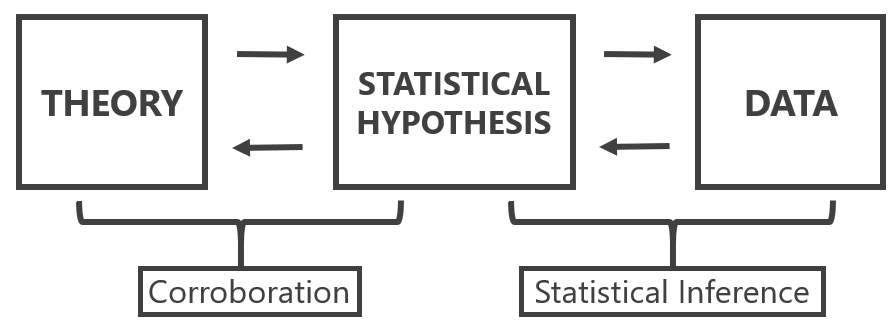
\includegraphics[width=1\linewidth]{images/meehl1990} 

}

\caption{Distinction between a theoretical hypothesis, a statistical hypothesis, and observations. Figure based on Meehl, 1990.}\label{fig:meehl1990}
\end{figure}

\hypertarget{loosening-and-tightening}{%
\section{Loosening and Tightening}\label{loosening-and-tightening}}

For each of the three questions above, we can ask questions about description, prediction, and explanation during a \textbf{loosening} phase when doing research, or during a \textbf{tightening} phase \citep{fiedler_tools_2004}. The distinction is relative. During the loosening stage, the focus is on creating variation that provides the source for new ideas. During the tightening stage, selection takes place with the goal to distinguish useful variants from less useful variants. In descriptive research, an unstructured interview is more aligned with the loosening phase, while a structured interview is more aligned with the tightening phase. In prediction, building a prediction model based on the training set is the loosening phase, while evaluation the prediction error in the holdout dataset is the tightening phase. In explanation, exploratory experimentation functions to generate hypotheses, while hypothesis tests function to distinguish theories that make predictions that are corroborated from those theories which predictions are not corroborated.

It is important to realize whether your goal is to generate new ideas, or to test new ideas. Researchers are often not explicit about the stage their research is in, which runs the risk of trying to test hypotheses prematurely \citep{scheel_why_2021}. Clinical trials research is more explicit about the different phases of research, and distinguishes Phase 1, Phase 2, Phase 3, and Phase 4 trials. In a Phase 1 trial researchers evaluate the safety of a new drug or intervention in a small group of non-randomized (often healthy) volunteers, by examining how much of a drug is safe to give, while monitoring a range of possible side effects. A phase 2 trial are often performed with patients as participants, and can focus in more detail on finding the definite dose. The goal is to systematically explore a range of parameters (e.g., the intensity of a stimulus) to identify boundary conditions \citep{dubin_theory_1969}. A phase 3 trial is a large randomized controlled trial with the goal to test the effectiveness of the new intervention in practice. Phase 3 trials require a prespecified statistical analyses plan that strictly controls error rates. Finally, a Phase 4 trial examines long term safety and generalizability. Compared to a Phase 3 trial, there is more loosening, as researchers explore the possibility of interactions with other drugs, or moderating effects in certain subgroups of the population. In clinical trials, a Phase 3 trial requires a huge amount of preparation, and is not undertaken lightly.

\begin{figure}

{\centering 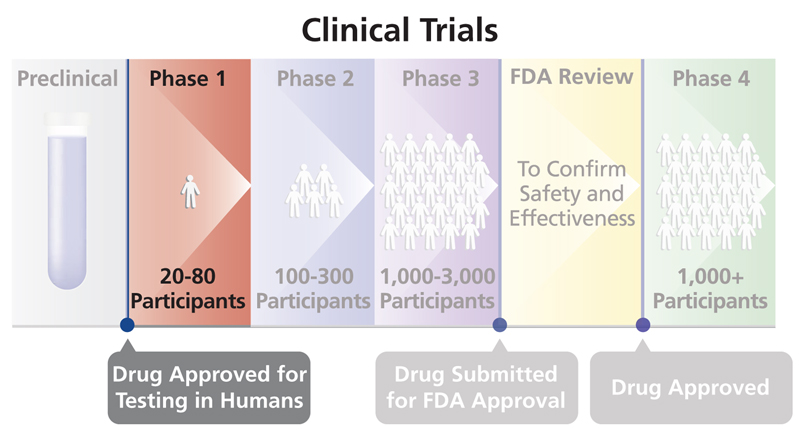
\includegraphics[width=1\linewidth]{images/trialphase} 

}

\caption{Four phases of clinical research. <a href="https://clinicalinfo.hiv.gov/en/glossary/phase-1-trial">Source</a>.}\label{fig:trialphase}
\end{figure}

\hypertarget{three-statistical-philosophies}{%
\section{Three statistical philosophies}\label{three-statistical-philosophies}}

Royall \citeyearpar{royall_statistical_1997} distinguishes three questions one can ask:

\begin{enumerate}
\def\labelenumi{\arabic{enumi}.}
\tightlist
\item
  What do I believe, now that I have this observation?
\item
  What should I do, now that I have this observation?
\item
  What does this observation tell me about A versus B? (How should I interpret this observation as evidence regarding A versus B?)
\end{enumerate}

One useful metaphor for thinking about these differences is if we look at Hinduism, where there are three ways to reach enlightenment: The Bhakti yoga, or the Path of Devotion, the Karma yoga, or the Path of Action, the Jnana yoga, or the Path of Knowledge. The three corresponding statistical paths are Bayesian statistics, which focuses on updating beliefs, Neyman-Pearson statistics, which focuses on making decisions about how to act, and likelihood approaches, which focus on quantifying the evidence or knowledge gained from the data. Just like in Hinduism the different paths are not mutually exclusive, and the emphasis on these three yoga's differs between individuals, so will scientists differ in their emphasis of their preferred approach to statistics.

The three approaches to statistical modelling (description, prediction, and explanation) can be examined from each the three statistical philosophies (e.g., frequentist estimation, maximum likelihood estimation, and Bayesian estimation, or Neyman-Pearson hypothesis tests, likelihood ratio tests, and Bayes factors). Bayesian approaches start from a specified prior belief, and use the data to update their belief. Frequentist procedures focus on methodological procedures that allow researchers to make inferences that control the probability of error in the long run. Likelihood approaches focus on quantifying the evidential value in the observed data. When used knowledgeably, these approaches often yield very similar inferences \citep{dongen_multiple_2019, lakens_improving_2020, tendeiro_review_2019}. Jeffreys \citeyearpar{jeffreys_theory_1939}, who developed a Bayesian hypothesis test, noted the following when comparing his Bayesian hypothesis test against frequentist methods proposed by Fisher:

\begin{quote}
I have in fact been struck repeatedly in my own work, after being led on general principles to a solution of a problem, to find that Fisher had already grasped the essentials by some brilliant piece of common sense, and that his results would be either identical with mine or would differ only in cases where we should both be very doubtful. As a matter of fact I have applied my significance tests to numerous applications that have also been worked out by Fisher's, and have not yet found a disagreement in the actual decisions reached.
\end{quote}

At the same time, each approach is based on different principles, and allows for specific inferences. For example, a Neyman-Pearson approach does not quantify evidence, and a Bayesian approach can lead conclusions about the relative support for one over another hypothesis, given specified priors, while ignoring the rate at which such a conclusion would be misleading. Understanding these basic principles is useful, as criticisms on statistical practices (e.g., computing \emph{p}-values) always boil down to a disagreement about the principles that different statistical philosophies are built on. However, when we survey the literature, we rarely see the viewpoint that all approaches to statistical inferences, including p values, provide answers to specific questions a researcher might want to ask. Instead, statisticians often engage in what I call the \textbf{statistician's
fallacy} --- a declaration of what they believe researchers really ``want to know'' without limiting the usefulness of their preferred statistical question to a specific context \citep{lakens_practical_2021}. The most well-known example of the statistician's fallacy is provided by Cohen \citeyearpar{cohen_earth_1994} when discussing null-hypothesis significance testing:

\begin{quote}
What's wrong with NHST? Well, among many other things, it does not tell us what we want to know, and we so much want to know what we want to know that, out of desperation, we nevertheless believe that it does! What we want to know is `Given these data, what is the probability that H0 is true?'
\end{quote}

Different statisticians will argue what you actually ``want to know'' is the posterior probability of a hypothesis, the false-positive risk, the effect size and its confidence interval, the likelihood, the Bayes factor, or the severity with which a hypothesis has been tested. However, it is up to you to choose a statistical strategy that matches the question you want the ask \citep{hand_deconstructing_1994}.

\hypertarget{do-you-really-want-to-test-a-hypothesis}{%
\section{Do You Really Want to Test a Hypothesis?}\label{do-you-really-want-to-test-a-hypothesis}}

A hypothesis test is a very specific answer to a very specific question. We can use a dart game as a metaphor for the question a hypothesis test aims to answer. In essence, both a dart game and a hypothesis test are a methodological procedure to make a directional prediction: Is A better or worse than B? In a dart game we very often compare two players, and the question is whether we should act as if player A is the best, or player B is the best. In a hypothesis test, we compare two hypotheses, and the question is whether we should act as if the null hypothesis is true, or whether the alternative hypothesis is true.

Historically, researchers have often been interested in testing hypotheses to examine whether predictions that are derived from a scientific theory hold up under scrutiny. Some philosophies of science (but not all) value theories that are able to make predictions. If a darter wants to convince you they are a good player, they can make a prediction (`the next arrow will hit the bulls-eye'), throw a dart, and impress you by hitting the bulls-eye. When a researcher uses a theory to make a prediction, collects data, and observes can claim based on a predefined methodological procedure that the results confirm their prediction, the idea is you are impressed by the \textbf{predictive validity of a theory} \citep{de_groot_methodology_1969}. The test supports the idea that the theory is a useful starting point to generate predictions about reality. Philosophers of science such as Popper call this `verisimilitude'-- the theory is in some way related to the truth, and it has some `truth-likeness'.

In order to be impressed when a prediction is confirmed, the prediction must be able to be wrong. In other words, a theoretical prediction needs to be falsifiable. If our predictions concern the presence or absence of clearly observable entities (e.g., the existence of a black swan) it is relatively straightforward to divide all possible states of the world into a set that is predicted by our theory (e.g., all swans are white), and a set that is not predicted by our theory (e.g., swans can have other colors than white). However, many scientific questions concern probabilistic events where single observations contain noise due to random variation -- rats have a certain probability to develop a tumor, people have a certain probability to buy a product, or particles have a certain probability to appear after a collision. If we want to forbid certain outcomes of our test when measuring probabilistic events, we can divide the states of the world based on the probability that some result will be observed.



\begin{figure}

{\centering 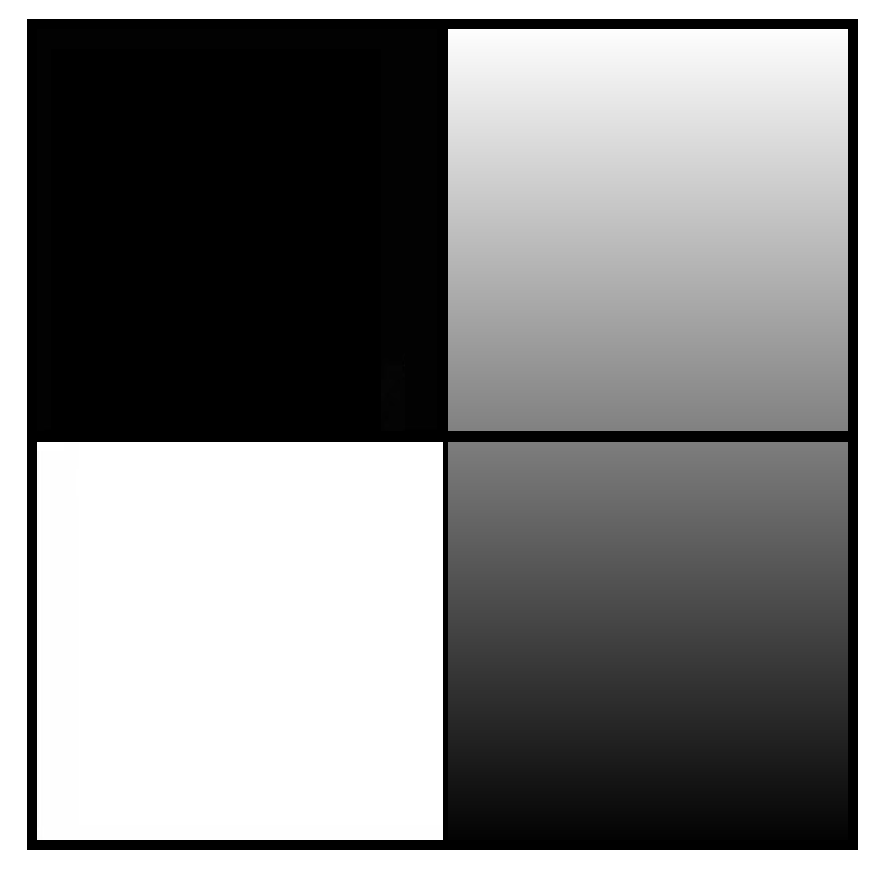
\includegraphics[width=1\linewidth]{images/blackwhite} 

}

\caption{Some fields make black and white predictions about the presence or absence of observables, but in many sciences, predictions are probabilistic, and shades of grey.}\label{fig:blackwhite}
\end{figure}

Just because a hypothesis test can be performed, does not mean it is interesting. A hypothesis test is most useful when 1) both data generating models that are decided between have some plausibility, and 2) it is possible to apply an informative methodological procedure.

First, the two competing models should both be good players. Just as in a dart game there would be very little interest if I played Michael van Gerwen (the world champion at the time of writing) to decide who the better dart player is. Since I do not play darts very well, a game between the two of us would not be interesting to watch. Similarly, it is sometimes completely uninteresting to compare two data generating models, one representing the state of the world when there is no effect, and another representing the state of the world when there is some effect, because in some cases the absence of an effect is extremely implausible.

Second, for a hypothesis test to be interesting you need to have designed an informative study. When designing a study, you need to be able to make sure that the methodological rule provides a severe test, where you are likely to corroborate a prediction if it is correct, while at the same time fail to corroborate a prediction when it is wrong \citep{mayo_statistical_2018}. If the world champion in darts and I stand 20 inches away from a dart board and can just push the dart in the location where we want it to end up, it is not possible to show my lack of skill. If we are both are blindfolded and throwing the darts from 100 feet, it is not possible for the world champion to display their skill. In a hypothesis test, the statistical severity of a test is determined by the error rates. Therefore, a researcher needs to be able to adequately control error rates to perform a test of a hypothesis with high informational value.

By now it is hopefully clear that hypothesis tests are a very specific tool, that answer a very specific question: After applying a methodological rule to observed data, which decision should I make if I do not want to make incorrect decisions too often? If you have no desire to use a methodological procedure to decide between competing theories, there is no real reason to report the results of a hypothesis test. Even though it might feel like you should test a hypothesis when doing research, carefully thinking about the statistical question you want to ask might reveal that alternative statistical approaches, such as describing the data you have observed, quantifying your personal beliefs about hypotheses, or reporting the relative likelihood of data under different hypotheses might be the approach that answers the question you really want to know.

\hypertarget{onesided}{%
\section{Directional (One-Sided) versus Non-Directional (Two-Sided) Tests}\label{onesided}}

Interestingly, there is quite some disagreement about whether the statistical question you ask in a study should be \textbf{directional} (meaning that only effects in a predicted direction will lead to rejection of the null hypothesis) or \textbf{non-directional} (meaning that effects in either direction will lead to the rejection of the null-hypothesis). For example, \citet{baguley_serious_2012} writes ``one-sided tests should typically be avoided'' because researchers are rarely willing to claim an effect in the non-predicted direction is non-significant, regardless of how large it is. At the same time, \citet{jones_test_1952} has stated: ``Since the test of the null hypothesis against a one-sided alternative is the most powerful test for all directional hypotheses, it is strongly recommended that the one-tailed model be adopted wherever its use is appropriate'', and \citet{cho_is_2013} complain about the ``widespread overuse of two-tailed testing for directional research hypotheses tests''. Let's reflect on some arguments for or against the choice to perform a one-sided test.

First, it is clear that a directional test provides a clear advantage in statistical power. As Figure \ref{fig:onesidedtwosidedratio} shows, the ratio of the sample for a non-directional versus a directional test means that approximately 80\% of the sample size of a non-directional test is required to achieve the same power in a directional test (the exact benefit depends on the power and effect size, as seen in the figure below).



\begin{figure}

{\centering 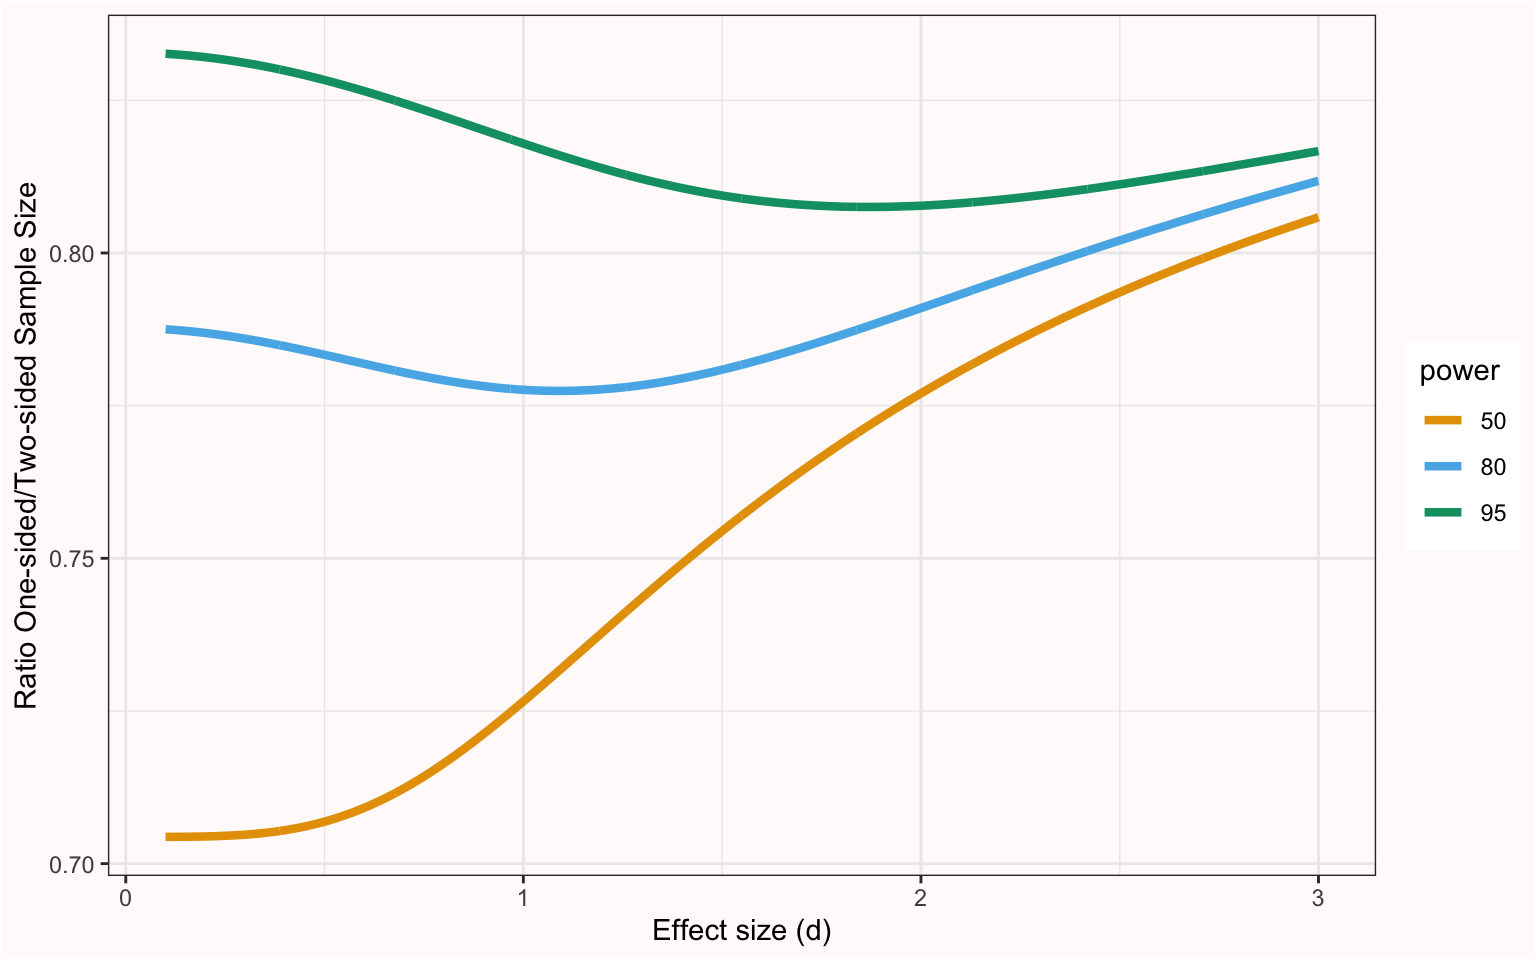
\includegraphics[width=1\linewidth]{05-questions_files/figure-latex/onesidedtwosidedratio-1} 

}

\caption{Ratio of the required sample size for a one-sample \emph{t}-test for a non-directional/directional test to achieve 50\%, 80\% or 95\% power.}\label{fig:onesidedtwosidedratio}
\end{figure}

Because in a directional test the alpha level is used for only one tail of the distribution, the critical test value is lower, and all else equal, power is higher. This reduction of the critical value required to declare a statistically significant effect has been criticized because it leads to weaker evidence. For example, \citet{schulz_sample_2005} write: ``Using a one-sided test in sample size calculations to reduce required sample sizes stretches credulity.''. This is trivially true: Any change to the design of a study that requires a smaller sample size reduces the strength of the evidence you collect, since the strength of evidence is inherently tied to the total number of observations. However, it conflates two types of statistical philosophies, namely a likelihoodist approach, which aims to quantify relative evidence, and a frequentist approach, which aims to provide a procedure to make claims with a maximum error rate. There is a difference between designing a study that yields a certain level of evidence, and a study that adequately controls the error rates when performing a hypothesis test. If you desire a specific level of evidence, design a study that provides this desired level of evidence. If you desire to control the error rate of claims, then that error rate is at most 5\% as long as the alpha level is 5\%, regardless of whether a one-sided or two-sided test is performed.

Note that there is a subtle distinction between a directional and a one-sided test \citep{baguley_serious_2012}. Although the two terms overlap when performing a \emph{t}-test, they do not overlap for an \emph{F}-test. The \emph{F}-value and the \emph{t}-value are related: \(t^2 = F\). This holds as long as the df1 = 1 (e.g., F(1, 100), or in other words as long as only two groups are compared. We can see in Figure \ref{fig:fandt} that the two distributions touch at t = 1 (as 1\^{}2 = 1), and that the \emph{F}-test has no negative values due to the squared nature of the distribution. The critical \emph{t}-value, squared, of a non-directional \emph{t}-test with a 5\% error rate equals the critical \emph{F}-value for an \emph{F}-test, which is always one-sided, with a 5\% error rate. Due to the `squared' nature of an \emph{F}-test, an \emph{F}-test is always non-directional. You can logically not halve the \emph{p}-value in an \emph{F}-test to perform a `one-sided' test, because you can't have a directional \emph{F}-test. When comparing two groups, you can use a \emph{t}-test instead of an \emph{F}-test, which can be directional.



\begin{figure}

{\centering 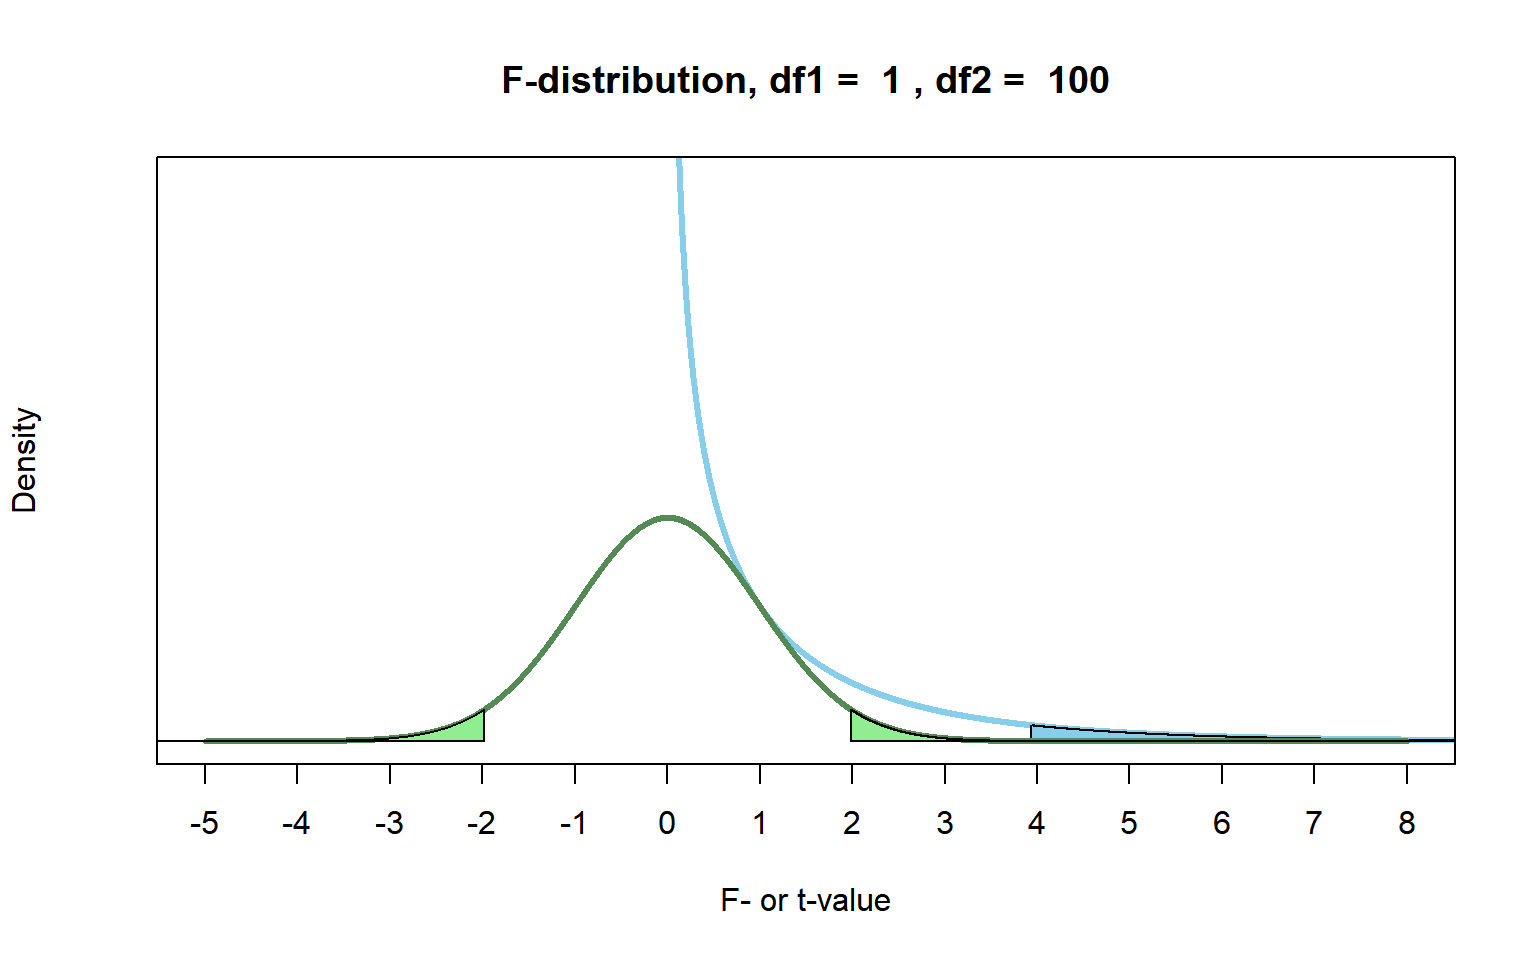
\includegraphics[width=1\linewidth]{05-questions_files/figure-latex/fandt-1} 

}

\caption{Distribution and rejection areas for a two-sided t-test and the corresponding F-test with df1 = 1 and df2 = 100.}\label{fig:fandt}
\end{figure}

A final concern raised against one-sided tests is that surprising findings in the opposite direction might be meaningful, and should not be ignored. I agree, but this is not an argument against one-sided testing. The goal in hypothesis testing is, not surprisingly, to test a hypothesis. If you have a directional hypothesis, a result in the opposite direction can never confirm your hypothesis. It can lead one to create a new hypothesis, but this new hypothesis should be tested on a new dataset \citep{de_groot_methodology_1969}.
It makes sense to \emph{describe} an unexpected effect in the opposite direction of your prediction, but there is a difference between describing data, and testing a hypothesis. A one-sided hypothesis test does not prohibit researchers from describing unexpected data patterns. And if you really want to test if there is an effect in either direction, simply preregister a two-sided test.

\hypertarget{crud}{%
\section{Systematic Noise, or the Crud Factor}\label{crud}}

Meehl \citeyearpar{meehl_theoretical_1978} believes ``the almost universal reliance on merely refuting the null hypothesis as the standard method for corroborating substantive theories in the soft areas is a terrible mistake, is basically unsound, poor scientific strategy, and one of the worst things that ever happened in the history of psychology''. At the same time, he also wrote: ``When I was a rat psychologist, I unabashedly employed significance testing in latent-learning experiments; looking back I see no reason to fault myself for having done so in the light of my present methodological views'' \citep{meehl_appraising_1990}. When he asks `Is it ever correct to use null-hypothesis significance tests?' his own answer is:

\begin{quote}
Of course it is. I do not say significance testing is never appropriate or helpful; there are several contexts in which I would incline to criticize a researcher who failed to test for significance.
\end{quote}

Meehl is not of the opinion that null hypothesis significance tests are not useful at all, but that the question if \emph{any} difference from zero exists is sometimes not a very interesting question to ask. Crucially, Meehl is especially worried about the widespread use of null hypothesis significance tests where there is room for \textbf{systematic noise}, or the \textbf{crud factor} in the data that are analyzed. The presence of systematic noise in data means that it is extremely unlikely that the null hypothesis is true, and combined with a large enough dataset, the question whether the null hypothesis can be rejected is uninteresting.

Systematic noise can only be excluded in an ideal experiment. In this ideal experiment, only one single factor can lead to an effect, such as in a perfect \textbf{randomized controlled trial}. Perfection is notoriously difficult to achieve in practice. In any not perfect experiment, there can be tiny causal factors that, although not being the main goal of the experiment, lead to differences between the experimental and control condition. Participants in the experimental condition might read more words, answer more questions, need more time, have to think more deeply, or process more novel information. Any of these things could slightly move the true effect size away from zero -- without being related to the independent variable the researchers aimed to manipulate. The difference is reliable, but not caused by anything the researcher is \textbf{theoretically interested} in. In real life, experiments are not even close to perfect. Consequently, there is always some room for systematic noise, although there is no way to know how large this systematic noise is in any specific study.

Systematic noise is especially a problem in studies where there is no randomization, such as in correlational studies. As an example of correlational data, think about research that examines differences between women and men. In such a study the subjects cannot be randomly assigned to each condition. In such non-experimental studies, it is possible that `\textbf{everything is correlated to everything}'. Or slightly more formally, crud can be defined as the epistemological concept that, in correlational research, all variables are connected through multivariate causal structures which result in real non-zero correlations between all variables in any given dataset \citep{orben_crud_2020}. For example, men are on average taller than women, and as a consequence men will be asked by strangers to pick an object from a high shelf in a supermarket a bit more often tham women. If we ask men and women `how often do you help strangers' this average difference in height has some tiny but systematic effect on their responses, even though a researcher might be theoretically interested in differences unrelated to height. In this specific case, systematic noise moves the mean difference from zero to a slightly higher value for men -- but an unknown number of other sources of systematic noise are at play, and these all interact, leading to an unknown final true population difference that is very unlikely to be exactly zero.

As a consequence, some scientific fields find tests of correlations relatively uninteresting. Researchers in these fields might find it interesting to \emph{estimate} the size of correlations, but they might not find it worthwhile to perform a null hypothesis significance \emph{test} for a correlation, as with a large enough dataset, statistical significance is practically guaranteed. This is increasingly true, the bigger the dataset. As an anecdote, while working on a paper on \protect\hyperlink{sequential}{sequential analysis}, I asked my collaborator Prof.~Wassmer why the \texttt{rpact} package did not have a module for tests of correlations. He replied that there was not enough interest in null hypothesis significance tests for correlations in biopharmaceutical statistics, because as everything correlates with everything anyway, why would anyone want to test it?

When you perform a nil null hypothesis test, you should justify why the nil null hypothesis is an interesting hypothesis to test against. This is not always self-evident, and sometimes the nil null hypothesis is simply not very interesting. Is it plausible that the nil null hypothesis is true? If not, then it is more interesting to perform a \protect\hyperlink{MET}{minimal effect test}. For a concrete example of how to determine if the presence of crud warrants the use of minimal effect tests in a literature, see \citet{ferguson_providing_2021}.

Several Registered Replication Reports in psychology have shown that for for all practical purposes, and given the sample sizes psychologists are able to collect, it has sometimes proven surprisingly difficult to reject the null hypothesis. A multilab replication study examining the action-sentence compatibility effect showed an average effect on the logarithm of the lift-off times close to 0 {[}-0.006, 0.004{]} in 903 native English speakers \citep{morey_pre-registered_2021}. A Registered Replication Report examining the effect of priming participants with either professor or hooligan related concepts yielded a non-significant difference in the number of general knowledge questions answered of a difference of 0.14\% {[}−0.71\%, 1.00\%{]} in a sample of 4493 participants \citep{odonnell_registered_2018}. A Registered Replication Report examining the effect of recalling the ten commandments or 10 books read in highschool on how often people cheated on a problem-solving task showed a non-significant difference of 0.11 {[}-0.09; 0.31{]} matrices in a sample of 4674 participants \citep{verschuere_registered_2018}. A Registered Replication Report testing the facial feedback hypothesis showed a non-significant effect on funniness ratings between conditions where participants were manipulated to move muscles related to smiling or pouting of 0.03 {[}−0.11; 0.16{]} scale units in a sample of 1894 participants \citep{wagenmakers_registered_2016}. A multi-lab replication study of the ego-depletion effect (which will feature more prominently in the chapter on \protect\hyperlink{bias}{bias}) observed an effect of \emph{d} = 0.04 {[}−0.07, 0.15{]} in a sample of 2141 participants \citep{hagger_multilab_2016}. These studies suggest that sometimes the nil null hypothesis is a plausible model to test against, and that even with sample sizes much larger than are typically collected in psychological research, the nil null is surprisingly difficult to reject.

Other multi-lab studies provide indications of tiny true effects, which could be due to the crud factor. \citet{colling_registered_2020} observed congruency effects in the attentional SNARC effect for four inter-stimulus interval conditions (250, 500, 750, and 1000 ms) of -0.05 ms {[}-0.82l; 0.71{]}, 1.06 ms {[}0.34; 1.78{]}, 0.19 ms {[}-0.53; 0.90{]}, and 0.18 ms {[}-0.51; 0.88{]} with a sample size of 1105 participants. For the statistically significant effect in the 500 ms ISI condition (which might be crud) they conclude: ``we view a difference of about 1 ms, even if ``real,'' as too small for any neurally or psychologically plausible mechanism---particularly one constrained to operate only within a narrow time window of 500 ms after the stimulus.'' \citet{mccarthy_registered_2018} observed a difference of 0.08 {[}0.004; 0.16{]} in how hostile ambiguous behavior in a vignette was rated after a priming task where more or less words were related to hostility, and conclude ``Our results suggest that the procedures we used in this replication study are unlikely to produce an assimilative priming effect that researchers could practically and routinely detect.'' In these instances, the null-hypothesis can be rejected, but the observed effect size is deemed too small to matter. As discussed in the chapter on equivalence testing and interval hypotheses, the solution to this problem is to specify a \protect\hyperlink{sesoi}{smallest effect size of interest}.

\hypertarget{effectsize}{%
\chapter{Effect Sizes}\label{effectsize}}

Effect sizes are an important statistical outcome in most empirical studies. Researchers want to know whether an intervention or experimental manipulation has an effect greater than zero, or (when it is obvious an effect exists) how big the effect is. Researchers are often reminded to report effect sizes, because they are useful for three reasons. First, they allow researchers to present the magnitude of the reported effects, which allow researchers to reflect on the \textbf{practical significance} of the effects they report, in addition to the \emph{statistical} significance. Second, effect sizes allow researchers to draw meta-analytic conclusions by comparing standardized effect sizes across studies. Third, effect sizes from previous studies can be used when planning a new study in an a-priori power analysis.

A measure of effect size is a quantitative description of the strength of a phenomenon. It is expressed as a number on a scale. For \textbf{unstandardized effect sizes}, the effect size is expressed on the scale that the measure was collected on. This is useful whenever people are able to intuitively interpret differences on a measurement scale. For example, children grow on average 6 centimeters a year between the age of 2 and puberty. We can interpret 6 centimeters a year as an effect size, and many people in the world have an intuitive understanding of how large 6 cm is. Where a \emph{p}-value is used to make a claim about whether there is an effect, or whether we might just be looking at random variation in the data, an effect size is used to answer the question how large the effect is. This makes an effect size estimate an important complement to \emph{p}-values in most studies. A \emph{p}-value tells us we can claim children grow as they age; effect sizes tell us what size clothes we can expect children to wear when they are a certain age, and how long it will take before their new clothes are too small.

For people in parts of the world that do not use the metric system, it might be difficult to understand what a difference of 6 cm is. To facilitate a comparison of effect sizes across situations where different measurement scales are used, researchers can report \textbf{standardized effect sizes}. A standardized effect size, such as \textbf{Cohen's \emph{d}}, is computed by dividing the difference on the raw scale by the standard deviation, and is thus scaled in terms of the variability of the sample from which it was taken. An effect of \emph{d} = 0.5 means that the difference is the size of half a standard deviation of the measure. This means that effect sizes are determined both by the size of an effect and the size of the standard deviation, and difference in a standardized effect size can be caused by a difference in the size of the unstandardized effect, or by a difference in the standard deviation.

Standardized effect sizes are common when variables are not measured on a scale people are familiar with, or are measured on different scales within the same research area. If you ask people how happy they are, an answer of `5' will mean something very different if you asked people to answer on a scale from 1 to 5 than if you asked them to answer on a scale from 1 to 9. Standardized effect sizes can be understood and compared regardless of the scale that was used to measure the dependent variable. Despite the ease of use of standardized effect size measures, there are good arguments to report and interpret unstandardized effect sizes wherever possible \citep{baguley_standardized_2009}.

Standardized effect sizes can be grouped in two families (Rosenthal, 1994): The \emph{d} family (consisting of standardized mean differences) and the \emph{r} family (measures of strength of association). Conceptually, the d family effect sizes are based on the difference between observations, divided by the standard deviation of these observations. The r family effect sizes describe the proportion of variance that is explained by group membership. For example, a correlation (\(r\)) of 0.5 indicates 25\% of the variance (\(r^2\)) is explained by the difference between groups. These effect sizes are calculated from the sum of squares (the difference between individual observations and the mean for the group, squared, and summed) for the effect divided by the sums of squares for other factors in the design.

\hypertarget{effect-sizes}{%
\section{Effect sizes}\label{effect-sizes}}

What is the most important outcome of an empirical study? You might be tempted to say it's the \emph{p}-value of the statistical test, given that it is practically always reported in articles, and determines whether we call something `significant' or not. However, as \citet{cohen_things_1990} writes in his `Things I've learned (so far)':

\begin{quote}
I have learned and taught that the primary product of a research inquiry is one or more measures of effect size, not \emph{p}-values.
\end{quote}

Although what you want to learn from your data is different in every study, and there rarely is any single thing you always want to know, effect sizes are a very important part of the information we gain from data collection.

A measure of effect size is a ``quantitative reflection of the magnitude of some phenomenon that is used for the purpose of addressing a question of interest'' \citep{kelley_effect_2012}. It is expressed as a number on a scale, and which scale is used depends on the effect size measure that is used. For \textbf{unstandardized effect sizes}, we can use a scale that people are very familiar with. For example, children grow on average 6 centimeters a year between the age of 2 and puberty. We can interpret 6 centimeters a year as an effect size. It is obvious an effect size has many benefits over a \emph{p}-value. A \emph{p}-value gives an indication that it is very unlikely children stay the same size as they become older -- effect sizes tell us what size clothes we can expect children to wear when they are a certain age, and how long it will take before their new clothes are too small.

One reason to report effect sizes is to facilitate future research. It is possible to perform a meta-analysis or a power analysis based on unstandardized effect sizes and their standard deviation, but it is easier to work with standardized effect sizes, especially when there is variation in the measures researchers use. But the main goal of reporting effect sizes is to reflect on the question whether the observed effect size is meaningful. For example, we might be able to reliably measure that on average 19 years olds will grow 1 centimeter in the next year. This difference would be statistically significant in a large enough sample, but if you go shopping for clothes when you are 19 years old, it is not something you need care about. Let's look at two examples of studies where looking at the effect size, in addition to its statistical significance, would have improved the statistical inferences.

\hypertarget{the-facebook-experiment}{%
\section{The Facebook experiment}\label{the-facebook-experiment}}

In the summer of 2014 there were some concerns about an experiment Facebook had performed on its users to examine `emotional mood contagion', or the idea that people's moods can be influenced by the mood of people around them. You can read the article \href{http://www.pnas.org/content/111/24/8788.full}{here}. For starters, there was substantial concern about the ethical aspects of the study, primarily because the researchers who performed the study had not asked for \textbf{informed consent} from the participants in the study (you and me), nor did they ask for permission from the \textbf{institutional review board} (or ethics committee) of their university.

One of the other criticisms of the study was that it could be dangerous to influence people's mood. As Nancy J. Smyth, dean of the University of Buffalo's School of Social Work wrote on her \href{https://njsmyth.wordpress.com/2014/06/29/did-facebooks-secret-mood-manipulation-experiment-create-harm/}{Social Work blog}: ``There might even have been increased self-harm episodes, out of control anger, or dare I say it, suicide attempts or suicides that resulted from the experimental manipulation. Did this experiment create harm? The problem is, we will never know, because the protections for human subjects were never put into place''.

If this Facebook experiment had such a strong effect on people's mood that it made some people commit suicide who would otherwise not have committed suicide, this would obviously be problematic. So let us look at the effects the manipulation Facebook used had on people a bit more closely.

From the article, let's see what the researchers manipulated:

\begin{quote}
Two parallel experiments were conducted for positive and negative emotion: One in which exposure to friends' positive emotional content in their News Feed was reduced, and one in which exposure to negative emotional content in their News Feed was reduced. In these conditions, when a person loaded their News Feed, posts that contained emotional content of the relevant emotional valence, each emotional post had between a 10\% and 90\% chance (based on their User ID) of being omitted from their News Feed for that specific viewing.
\end{quote}

Then what they measured:

\begin{quote}
For each experiment, two dependent variables were examined pertaining to emotionality expressed in people's own status updates: the percentage of all words produced by a given person that was either positive or negative during the experimental period. In total, over 3 million posts were analyzed, containing over 122 million words, 4 million of which were positive (3.6\%) and 1.8 million negative (1.6\%).
\end{quote}

And then what they found:

\begin{quote}
When positive posts were reduced in the News Feed, the percentage of positive words in people's status updates decreased by B = −0.1\% compared with control {[}t(310,044) = −5.63, P \textless{} 0.001, Cohen's d = 0.02{]}, whereas the percentage of words that were negative increased by B = 0.04\% (t = 2.71, P = 0.007, d = 0.001). Conversely, when negative posts were reduced, the percent of words that were negative decreased by B = −0.07\% {[}t(310,541) = −5.51, P \textless{} 0.001, d = 0.02{]} and the percentage of words that were positive, conversely, increased by B = 0.06\% (t = 2.19, P \textless{} 0.003, d = 0.008).
\end{quote}

Here, we will focus on the negative effects of the Facebook study (so specifically, the increase in negative words people used) to get an idea of whether there is a risk of an increase in suicide rates. Even though apparently there was a negative effect, it is not easy to get an understanding about the size of the effect from the numbers as mentioned in the text. Moreover, the number of posts that the researchers analyzed was really large. With a large sample, it becomes important to check if the size of the effect is such that the finding is substantially interesting, because with large sample sizes even
minute differences will turn out to be statistically significant (we will look at this in more detail below). For that, we need a better understanding of ``effect sizes''.

\hypertarget{the-hungry-judges-study}{%
\section{The Hungry Judges study}\label{the-hungry-judges-study}}



\begin{figure}

{\centering \includegraphics[width=1\linewidth]{images/hungryjudges} 

}

\caption{Proportion of rulings in favor of the prisoners by ordinal position. Circled points indicate the first decision in each of the three decision sessions; tick marks on x axis denote every third case; dotted line denotes food break. From Danziger, S., Levav, J., Avnaim-Pesso, L. (2011). Extraneous factors in judicial decisions. Proceedings of the National Academy of Sciences, 108(17), 6889--6892. \url{https://doi.org/10.1073/PNAS.1018033108}}\label{fig:hungryjudges}
\end{figure}

We see a graphical representation of the proportion of favorable parole decisions that real-life judges are making as a function of the number of cases they process across the day in Figure \ref{fig:hungryjudges}. This study is mentioned in many popular science books as an example of a finding that shows that people do not always make rational decisions, but that ``judicial rulings can be swayed by extraneous variables that should have no bearing on legal decisions'' \citep{danziger_extraneous_2011}. We see that early on in the day, judges start by giving about 65\% of people parole, which basically means, ``All right, you can go back into society.'' But then very quickly, the number of favorable decisions decreases to basically zero. After a quick break which, as the authors say, ``may replenish mental resources by providing rest, improving mood, or by increasing glucose levels in the body'' the parole decisions are back up at 65\%, and then again quickly drop down to basically zero. They take another break, the percentage of positive decisions is back up to 65\%, only to drop again over the course of the day.

If we calculate the effect size for the drop after a break, and before the next break \citep{glockner_irrational_2016}, the effect represents a Cohen's \emph{d} of approximately two, which is incredibly large. There are hardly any effects in psychology this large, let alone effects of mood or rest on decision making. And this surprisingly large effect occurs not just once, but three times over the course of the day. If mental depletion actually has such a huge real-life impact, society would basically fall into complete chaos just before lunch break every day. Or at the very least, our society would have organized itself around this incredibly strong effect of mental depletion. Just like manufacturers take size differences between men and women into account when producing items such as golf clubs or watches, we would stop teaching in the time before lunch, doctors would not schedule surgery, and driving before lunch would be illegal. If a psychological effect is this big, we don't need to discover it and publish it in a scientific journal - you would already know it exists.

We can look at a meta-meta-analysis (a paper that meta-analyzes a large number of meta-analyses in the literature) by Richard, Bond, \& Stokes-Zoota \citeyearpar{richard_one_2003} to see which effect sizes in law psychology are close to a Cohen's \emph{d} of 2. They report two meta-analyzed effects that are slightly smaller. The first is the effect that a jury's final verdict is likely to be the verdict a majority initially favored, which 13 studies show has an effect size of \emph{r} = 0.63, or \emph{d} = 1.62. The second is that when a jury is initially split on a verdict, its final verdict is likely to be lenient, which 13 studies show to have an effect size of \emph{r} = .63 as well. In their entire database, some effect sizes that come close to \emph{d} = 2 are the finding that personality traits are stable over time (\emph{r} = 0.66, \emph{d} = 1.76), people who deviate from a group are rejected from that group (\emph{r} = .6, \emph{d} = 1.5), or that leaders have charisma (\emph{r} = .62, \emph{d} = 1.58). You might notice the almost tautological nature of these effects. And that is, supposedly, the effect size that the passing of time (and subsequently eating lunch) has on parole hearing sentencings.

We see how examining the size of an effect can lead us to identify findings that cannot be caused by their proposed mechanisms. The effect reported in the hungry judges study must therefore be due to a confound. Indeed, such confounds have been identified, as it turns out the ordering of the cases is not random, and it is likely the cases that deserve parole are handled first, and the cases that do not deserve parole are handled later \citep{weinshall-margel_overlooked_2011, chatziathanasiou_beware_2022}. An additional use of effect sizes is to identify effect sizes that are too large to be plausible. Hilgard \citeyearpar{hilgard_maximal_2021} proposes to build in `maximum positive controls', experimental conditions that show the largest possible effect that provides an upper limit on plausible effect size measures.

\hypertarget{cohend}{%
\section{Standardised Mean Differences}\label{cohend}}

Effect sizes can be grouped into two families \citep{rosenthal_contrasts_2000}: The \textbf{d family} (based on standardized mean differences) and the \textbf{r family} (based on measures of strength of association). Conceptually, the \emph{d} family effect sizes are based on a comparison between the difference between the observations, divided by the standard deviation of these observations. This means that a Cohen's \emph{d} = 1 means the standardized difference between two groups equals one standard deviation. The size of the effect in the Facebook study above was quantified with Cohen's \emph{d}. Cohen's \emph{d} (the \emph{d} is \href{https://blog.apastyle.org/apastyle/2011/08/the-grammar-of-mathematics-writing-about-variables.html}{italicized}) is used to describe the standardized mean difference of an effect. This value can be used to compare effects across studies, even when the dependent variables are measured with different scales, for example when one study uses 7-point scales to measure dependent variables, while the other study uses 9-point scales. We can even compare effect sizes across completely different measures of the same construct, one study uses a self-report measure, and another study uses a physiological measure. Although we can compare effect sizes across different measurements, this does not mean they are comparable, as we will discuss in more detail in the section on \protect\hyperlink{heterogeneity}{heterogeneity} in the chapter on meta-analysis.

Cohen's \emph{d} ranges from minus infinity to infinity (although in practice, the mean difference in the positive or negative direction that can be observed will never be infinite), with the value of 0 indicating there is no effect. Cohen \citeyearpar{cohen_statistical_1988} uses subscripts to distinguish different versions of Cohen's \emph{d}, a practice I will follow because it prevents confusion (without any specification, Cohen's \emph{d} denotes the entire family of effect sizes). Cohen refers to the standardized mean difference between two groups of independent observations for the \emph{sample} as \(d_s\). Before we get into the statistical details, let's first visualize what a Cohen's \emph{d} of 0.001 (as was found in the Facebook study) means. We will use a visualization from \url{http://rpsychologist.com/d3/cohend/}, a website made by Kristoffer Magnusson, that allows you to visualize the differences between two measurements (such as the increase in negative words used by the Facebook user when the number of positive words on the timeline was reduced). The visualization actually shows two distributions, one dark blue and one light blue, but they overlap so much that the tiny difference in distributions is not visible (click the settings button to change the slider settings, and set the step size to 0.001 to reproduce the figure below in the online app).



\begin{figure}

{\centering \includegraphics[width=1\linewidth]{images/rpsychd1} 

}

\caption{A vizualization of 2 groups (although the difference is hardly visible) representing d = 0.001.}\label{fig:rpsychd1}
\end{figure}

The four numbers below the distribution express the effect size in different ways to facilitate the interpretation. For example, the \textbf{probability of superiority} expresses the probability that a randomly picked observation from one group will have a larger score than a randomly picked observation from the other group. Because the effect is so small, this probability is 50.03\% - which means that people in the experimental write almost the same number of positive or negative words as people in the control condition. The \textbf{number needed to treat} index illustrates that in the Facebook study a person needs to type 3570 words before we will observe one additional negative word, compared to the control condition. I don't know how often you type this many words on Facebook, but I think we can agree this effect is not noticeable on an individual level.

To understand how Cohen's \emph{d} for two independent groups is calculated, let's first look at the formula for the \emph{t}-statistic:

\[
t = \frac{{\overline{M}}_{1}{- \overline{M}}_{2}}{\text{SD}_{\text{pooled}} \times \sqrt{\frac{1}{n_{1}} + \frac{1}{n_{2}}}}
\]

Here \({\overline{M}}_{1}{- \overline{M}}_{2}\) is the difference between the means, and \(\text{SD}_{\text{pooled}}\) is the pooled standard deviation \citep{lakens_calculating_2013}, and n1 and n2 are the sample sizes of the two groups that are being compared. The \emph{t}-value is used to determine whether the difference between two groups in a \emph{t}-test is statistically significant (as explained in the chapter on \protect\hyperlink{pvalue}{\emph{p}-values}. The formula for Cohen's \emph{d}\_ is very similar:

\[d_s = \frac{{\overline{M}}_{1}{-\overline{M}}_{2}}{\text{SD}_{\text{pooled}}}\]

As you can see, the sample size in each group (\(n_1\) and \(n_2\)) is part of the formula for a \emph{t}-value, but it is not part of the formula for Cohen's \emph{d} (the pooled standard deviation is computed by weighing the standard deviation in each group by the sample size, but it cancels out if groups are of equal size). This distinction is useful to know, because in practice it means that the \emph{t}-value (and consequently, the \emph{p}-value) is a function of the sample size, but Cohen's \emph{d} is independent of the sample size. If there is a true effect (e.g., a non-zero effect size in the population) the \emph{t}-value for a null hypothesis test against an effect of zero will on average become larger (and the \emph{p}-value will become smaller) as the sample size increases. The effect size, however, will not increase or decrease, but will become more accurate, as the standard error decreases as the sample size increases. This is also the reason why \emph{p}-values cannot be used to make a statement about whether an effect is \textbf{practically significant}, and effect size estimates are often such an important complement to \emph{p}-values when making statistical inferences.

You can calculate Cohen's \emph{d} for independent groups from the independent samples \emph{t}-value (which can often be convenient when the result section of the paper you are reading does not report effect sizes) through:

\[d_s = t ⨯ \sqrt{\frac{1}{n_{1}} + \frac{1}{n_{2}}}\]

A \emph{d} = 0.001 is an extremely tiny effect, so let's explore an effect size that is a bit more representative of what you would read in the literature. In the meta-meta-analysis mentioned earlier, the median effect size in published studies included in meta-analyses in the psychological literature is \emph{d} = 0.43 \citep{richard_one_2003}. To get a feeling for this effect size, let's use the online app and set the effect size to \emph{d} = 0.43.



\begin{figure}

{\centering \includegraphics[width=1\linewidth]{images/rpsychd2} 

}

\caption{A vizualization of 2 groups representing d = 0.43.}\label{fig:rpsychd2}
\end{figure}

One example of a meta-analytic effect size in the meta-meta-analysis that is exactly \(d_s\) = 0.43 is the finding that people in a group work less hard to achieve a goal than people who work individually, called \emph{social loafing}. This is an effect that is large enough that we notice it in daily life. Yet, if we look at the overlap in the two distributions, we see that the amount of effort people put in overlaps considerably between the two conditions (in the case of social loafing, working individually versus working in a group). We see in Figure \ref{fig:rpsychd2} that the \textbf{probability of superiority}, or the probability that if we randomly draw one person from the group condition and one person from the individual condition, the person working in a group puts in less effort, is only 61.9\%. This interpretation of differences between groups is also called the \textbf{common language effect size} \citep{mcgraw_common_1992}.



\begin{figure}

{\centering \includegraphics[width=1\linewidth]{images/rpsychd3} 

}

\caption{A vizualization of 2 groups representing d = 2.}\label{fig:rpsychd3}
\end{figure}

Based on \href{http://www.nature.com/pr/journal/v73/n3/full/pr2012189a.html}{this data}, the difference between the height of 21-year old men and women in The Netherlands is approximately 13 centimeters (in an unstandardized effect size), or a standardized effect size of \(d_s\) = 2. If I pick a random man and a random woman walking down the street in my hometown of Rotterdam, how likely is it that the man will be taller than the woman? We see this is quite likely, with a probability of superiority of 92.1\%. But even with such a huge effect, there is still considerable overlap in the two distributions. If we conclude the height of people in one group is greater than the height of people in another group, this does not mean everyone in one group is taller than everyone in the other group.

Sometimes when you try to explain scientific findings at a birthday party, a skeptical aunt or uncle might remark `well I don't believe that is true because \emph{I} never experience this'. With probabilistic observations, there is a distribution of observed effects. In the example about social loafing, \emph{on average} people put in less effort to achieve a goal when working in a group than working by themselves. For any individual in the population, the effect might be larger, smaller, absent, or even in the opposite direction. If your skeptical aunt or uncle never experiences a finding, this does not contradict the claim that the effect exists \emph{on average} in the population. Indeed, it is even expected that there is no effect for some people in the population, at least some of the time. Although there might be some exceptions (e.g., almost every individual will experience the \href{https://en.wikipedia.org/wiki/Stroop_effect}{Stroop effect}), many effects are smaller, or have sufficient variation, such that the effect is not present for every single individual in the population.

Conceptually, calculating Cohen's \emph{d} for within-subjects comparisons is based on the same idea as for independent groups, where the differences between two observations are divided by the standard deviation within the groups of observations. However, in the case of correlated samples the most common standardizer is the standard deviation of the difference scores. Testing whether two correlated means are significantly different from each other with a paired samples \emph{t}-test is the same as testing whether the difference scores of the correlated means is significantly different from 0 in a one-sample \emph{t}-test. Similarly, calculating the effect size for the difference between two correlated means is similar to the effect size that is calculated for a one sample \emph{t}-test. The standardized mean difference effect size for within-subjects designs is referred to as Cohen's \(d_z\), where the \emph{z} alludes to the fact that the unit of analysis is no longer \emph{x} or \emph{y}, but their difference, \emph{z}, and can be calculated with:

\[d_z = \frac{M_{dif}}{\sqrt{\frac{\sum{({X_{dif}-M_{dif})}}^2}{N-1}}}\]
The effect size estimate Cohen's \(d_z\) can also be calculated directly from the \emph{t}-value and the number of participants using the formula:

\[d_z = \frac{t}{\sqrt{n}}\]

Given the direct relationship between the \emph{t}-value of a paired-samples \emph{t}-test and Cohen's \(d_z\), it will not be surprising that software that performs power analyses for within-subjects designs (e.g., G*Power) relies on Cohen's \(d_z\) as input.

Maxwell \& Delaney \citeyearpar{maxwell_designing_2004} remark: `a major goal of developing effect size measures is to provide a standard metric that meta-analysts and others can interpret across studies that vary in their dependent variables as well as types of designs.' Because Cohen's \(d_z\) takes the correlation between the dependent measures into account, it cannot be directly compared with Cohen's \(d_s\). Some researchers prefer to use the average standard deviation of both groups of observations as a standardizer (which ignores the correlation between the observations), because this allows for a more direct comparison with Cohen's \(d_s\). This effect size is referred to as Cohen's \(d_{av}\) \citep{cumming_understanding_2013}, and is simply:

\[d_{av} = \frac{M_{dif}}{\frac{SD_1+SD_2}{2}}\]

\hypertarget{interpreting-effect-sizes}{%
\section{Interpreting effect sizes}\label{interpreting-effect-sizes}}

A commonly used interpretation of Cohen's \emph{d} is to refer to effect sizes as small (\emph{d} = 0.2), medium (\emph{d} = 0.5), and large (\emph{d} = 0.8) based on benchmarks suggested by Cohen (1988). However, these values are arbitrary and should not be used. In practice, you will only see them used in a form of circular reasoning: The effect is small, because it is \emph{d} = 0.2, and \emph{d} = 0.2 is small. We see that using the benchmarks adds nothing, beyond covering up the fact that we did not actually interpret the size of the effect. Furthermore, benchmarks for what is a `medium' and `large' effect do not even correspond between Cohen's \emph{d} and \emph{r} (as explained by \citet{mcgrath_when_2006}, see the `Test Yourself' Q12). Any verbal classification based on benchmarks ignores the fact that any effect can be practically meaningful, such as an intervention that leads to a reliable reduction in suicide rates with an effect size of \emph{d} = 0.1. In other cases, an effect size of \emph{d} = 0.1 might have no consequence at all, for example because such an effect is smaller than the just noticeable difference, and is therefore too small to be noticed by individuals in the real world.

Publication bias and flexibility in the data analysis inflate effect size estimates. Innovations such as Registered Reports \citep{chambers_past_2022, nosek_registered_2014} increasingly lead to the availability of unbiased effect size estimates in the scientific literature. One consequence is that many effect sizes will turn out to be smaller than researchers thought. For example, in the 100 replication studies performed in the Reproducibility Project: Psychology, observed effect sizes in replication studies were on average half the size as those observed in the original studies \citep{open_science_collaboration_estimating_2015}.

To not just \emph{report} but \emph{interpret} an effect size, nothing is gained by the common practice of finding the corresponding verbal label of `small', `medium', or `large'. Instead, researchers who want to argue that an effect is meaningful need to provide empirical and falsifiable arguments for the meaningfulness of effects \citep{primbs_are_2022, anvari_not_2021}. One approach to argue effect sizes are meaningful is by explicitly specifying a \protect\hyperlink{sesoi}{smallest effect size of interest}{]} \citep{gotz_small_2022}, for example based on a cost-benefit analysis. Alternatively, researchers can interpret effect sizes relative to other effects in the literature \citep{baguley_standardized_2009, funder_evaluating_2019}.

\hypertarget{correlations-and-variance-explained}{%
\section{Correlations and Variance Explained}\label{correlations-and-variance-explained}}

The \emph{r} family effect sizes are based on the proportion of variance that is explained by group membership (e.g., a correlation of \emph{r} = 0.5 indicates 25\% of the variance (\(r^2\) is explained by the difference between groups). You might remember that \emph{r} is used to refer to a correlation. The correlation of two continuous variables can range from 0 (completely unrelated) to 1 (perfect positive relationship) or -1 (perfect negative relationship). To get a better feel of correlations, play the game \href{http://guessthecorrelation.com/}{guess the correlation} where you will see a scatterplot, and have to guess the correlation between the variables (see figure \ref{fig:guesscorrelation}.



\begin{figure}

{\centering \includegraphics[width=1\linewidth]{images/guesscorrelation} 

}

\caption{Screenshot from Guess the Correlation game (the correct answer is r = 0.24).}\label{fig:guesscorrelation}
\end{figure}

The \emph{r} family effect sizes are calculated from the sum of squares (the difference between individual observations and the mean for the group, squared, and summed) for the effect divided by the sums of squares for other factors in the design. Earlier, I mentioned the median effect size in psychology is \(d_s\) = 0.43. However, the authors actually report their results as a correlation, \emph{r} = 0.21. We can convert Cohen's \emph{d} into \emph{r} (but take care that this only applies to \(d_s\), not \(d_z\)):

\[r = \frac{d_s}{\sqrt{{d_s^{2}}^{+}\frac{N^{2} - 2N}{n_{1} \times n_{2}}}}\]

\emph{N} is the total sample size of both groups, whereas \(n_1\) and \(n_2\) are the sample sizes of the individual groups you are comparing (it is common to use capital \(N\) for the total sample size, and lowercase n for sample sizes per group). You can go to \url{http://rpsychologist.com/d3/correlation/} to look at a good visualization of the proportion of variance that is explained by group membership, and the relationship between \emph{r} and \(r^2\). The amount of variance explained is often quite a small number, and we see in Figure \ref{fig:sharedvariance} that a correlation of 0.21 (the median from the meta-meta-analysis by Richard and colleagues) we see the proportion of variance explained is only 4.4\%. Funder and Ozer \citeyearpar{funder_evaluating_2019} warn against misinterpreting small values for the variance explained as an indication that the effect is not meaningful (and they even consider the practice of squaring the correlation ``actively misleading'').



\begin{figure}

{\centering \includegraphics[width=1\linewidth]{images/sharedvariance} 

}

\caption{Screenshot from correlation effect size vizualization by Kristoffer Magnusson for r = 0.21.}\label{fig:sharedvariance}
\end{figure}

As we have seen before, it can be useful to interpret effect sizes to identify effects that are practically insignificant, or effects that are implausibly large. Let's take a look at a study that examines the number of suicides as a function of the amount of country music played on the radio. You can find the paper \href{https://heinonline.org/HOL/P?h=hein.journals/josf71\&i=227}{here} It won an \href{http://www.abc.net.au/science/articles/2004/10/01/1211441.htm}{Ig Nobel prize for studies that first make you laugh, and then think}, although in this case, the the study should not make you think about country music, but about the importance of interpreting effect sizes.

The authors predicted the following:

\begin{quote}
We contend that the themes found in country music foster a suicidal mood among people already at risk of suicide and that it is thereby associated with a high suicide rate.
\end{quote}

Then they collected data:

\begin{quote}
Our sample is comprised of 49 large metropolitan areas for which data on music were available. Exposure to country music is measured as the proportion of radio airtime devoted to country music. Suicide data were extracted from the annual Mortality Tapes, obtained from the Inter-University Consortium for Political and Social Research (ICPSR) at the University of Michigan. The dependent variable is the number of suicides per 100,000 population.
\end{quote}

And they concluded:

\begin{quote}
A significant zero-order correlation was found between white suicide rates and country music (\emph{r} = .54, \emph{p} \textless{} .05). The greater the airtime given to country music, the greater the white suicide rate.
\end{quote}

We can again compare the size of this effect with other known effects in psychology. In the database by Richard and colleagues, there are very few effects this large, but some examples are: that leaders are most effective if they have charisma (\emph{r} = 0.54), good leader--subordinate relations promote subordinate satisfaction (\emph{r} = 0.53), and people can recognize emotions across cultures (\emph{r} = 0.53). These effects are all large and obvious, which should raise some doubts about whether the relationship between listening to country music and suicides can be of the same size. Is country music really that bad? If we search the literature, we find that \href{http://sf.oxfordjournals.org/content/74/1/327.short}{other researchers were not able to reproduce the analysis of the original authors}. It is likely that the results are spurious, or a Type 1 error.

Eta squared \(\eta^2\) (part of the \emph{r} family of effect sizes, and an extension of r that can be used for more than two sets of observations) measures the proportion of the variation in Y that is associated with membership of the different groups defined by X, or the sum of squares of the effect divided by the total sum of squares:

\[\eta^{2} = \frac{\text{SS}_{\text{effect}}}{\text{SS}_{\text{total}}}\]

An \(\eta^2\) of .13 means that 13\% of the total variance can be accounted for by group membership. Although \(\eta^2\) is an efficient way to compare the sizes of effects within a study (given that every effect is interpreted in relation to the total variance, all \(\eta^2\) from a single study sum to 100\%), eta squared cannot easily be compared between studies, because the total variability in a study (\(SS_{total}\)) depends on the design of a study, and increases when additional variables are manipulated (e.g., when independent variables are added). Keppel \citep{keppel_design_1991} has recommended partial eta squared (\(\eta_{p}^{2}\)) to improve the comparability of effect sizes between studies. \(\eta_{p}^{2}\) expresses the sum of squares of the effect in relation to the sum of squares of the effect plus the sum of squares of the error associated with the effect. Partial eta squared is calculated as:

\[\eta_{p}^{2} = \frac{\text{SS}_{\text{effect}}}{\text{SS}_{\text{effect}} + \text{SS}_{\text{error}}}\]

For designs with fixed factors (manipulated factors, or factors that exhaust all levels of the independent variable, such as alive vs.~dead), but not for designs with measured factors or covariates, partial eta squared can be computed from the \emph{F}-value and its degrees of freedom \citep{cohen_statistical_1988}:

\[\eta_{p}^{2} = \frac{F \times \text{df}_{\text{effect}}}{{F \times \text{df}}_{\text{effect}} + \text{df}_{\text{error}}}\]

For example, for an \emph{F}(1, 38) = 7.21, \(\eta_{p}^{2}\) = 7.21 ⨯ 1/(7.21 ⨯ 1 +
38) = 0.16.

Eta squared can be transformed into Cohen's \emph{d}:

\emph{d} = 2\(\times f\) where \(f^{2} = \eta^{2}/(1 - \eta^{2})\)

\hypertarget{correcting-for-bias}{%
\section{Correcting for Bias}\label{correcting-for-bias}}

Population effect sizes are almost always estimated on the basis of samples, and as a measure of the population effect size estimate based on sample averages, Cohen's \emph{d} slightly overestimates the true population effect. When Cohen's \emph{d} refers to the population, the Greek letter δ is typically used. Therefore, corrections for bias are used (even though these corrections do not always lead to a completely unbiased effect size estimate). In the \emph{d} family of effect sizes, the correction for bias in the population effect size estimate of Cohen's \emph{d} is known as Hedges' \emph{g} (although different people use different names -- \(d_{unbiased}\) is also used). This correction for bias is only noticeable in small sample sizes, but since we often use software to calculate effect sizes anyway, it makes sense to always report Hedge's \emph{g} instead of Cohen's \emph{d} \citep{thompson_effect_2007}.

As with Cohen's \emph{d}, \(\eta^2\) is a biased estimate of the true effect size in the population. Two less biased effect size estimates have been proposed, epsilon squared \(\varepsilon^{2}\) and omega squared \(\omega^{2}\). For all practical purposes, these two effect sizes correct for bias equally well \citep{okada_is_2013, albers_when_2018}, and should be preferred above \(\eta^2\). Partial epsilon squared (\(\varepsilon_{p}^{2}\)) and partial omega squared (\(\omega_{p}^{2}\)) can be calculated based on the \emph{F}-value and degrees of freedom.

\[
\omega_{p}^{2} = \frac{F - 1}{F + \ \frac{\text{df}_{\text{error}} + 1}{\text{df}_{\text{effect}}}}
\]

\[
\varepsilon_{p}^{2} = \frac{F - 1}{F + \ \frac{\text{df}_{\text{error}}}{\text{df}_{\text{effect}}}}
\]
Partial effect sizes \(\eta_{p}^{2}\), \(\varepsilon_{p}^{2}\) and \(\omega_{p}^{2}\) cannot be generalized across different designs. For this reason, generalized eta-squared (\(\eta_{G}^{2}\)) and generalized omega-squared (\(\omega_{G}^{2}\)) have been proposed \citep{olejnik_generalized_2003}, although they are not very popular. In part, this might be because summarizing the effect size in an ANOVA design with a single index has limitations, and perhaps it makes more sense to describe the pattern of results, as we will see in the section below.

\hypertarget{effect-sizes-for-interactions}{%
\section{Effect Sizes for Interactions}\label{effect-sizes-for-interactions}}

The effect size used for power analyses for ANOVA designs is Cohen's \emph{f}. For two independent groups, Cohen's \(f\) = 0.5 * Cohen's \emph{d}. For more than two groups, Cohen's f can be converted into eta-squared and back with \(f = \frac{\eta^2}{(1 - \eta^2)}\) or \(\eta^2 = \frac{f^2}{(1 + f^2)}\). When predicting interaction effects in ANOVA designs, planning the study based on an expected effect size such as \(\eta_{p}^{2}\) or Cohen's \emph{f} might not be the most intuitive approach.

Let's start with the effect size for a simple two group comparison. Let's assume we predict a mean difference of 1, and know the standard deviation of the measure is 2. This means the standardized effect size is \emph{d} = 0.5. An independent \emph{t}-test is mathematically identical to an \emph{F}-test with two groups. For an \emph{F}-test, the effect size used for power analyses is Cohen's \emph{f}, which is calculated based on the standard deviation of the population means divided by the population standard deviation (which we know for our measure is 2), or:

\begin{equation}
f = \frac{\sigma _{ m }}{\sigma}
\end{equation}
where for equal sample sizes
\begin{equation}
\sigma _{ m } = \sqrt { \frac { \sum_ { i = 1 } ^ { k } ( m _ { i } - m ) ^ { 2 } } { k } }.
\end{equation}

In this formula \emph{m} is the grand mean, k is the number of means, and m\_i is the mean in each group. The formula above might look a bit daunting, but calculating Cohen's f is not that difficult for two groups.

If we take the expected means of 0 and 1, and a standard deviation of 2, the grand mean (the \emph{m} in the formula above) is (0 + 1)/2 = 0.5. The formula says we should subtract this grand mean from the mean of each group, square this value, and sum them. So we have (0 - 0.5)\^{}2 and (1 - 0.5)\^{}2, which are both 0.25. We sum these values (0.25 + 0.25 = 0.5), divide them by the number of groups (0.5/2 = 0.25) and take the square root, we find that \(\sigma_{ m }\) = 0.5. We can now calculate Cohen's \emph{f} (using \(\sigma\) = 2 for our measure):

\begin{equation}
f = \frac{\sigma _{ m }}{\sigma} = \frac{0.5}{2} = 0.25
\end{equation}

We confirm that for two groups Cohen's \emph{f} is half as large as Cohen's \emph{d}.

Now we have the basis to look at interaction effects. Different patterns of means in an ANOVA can have the same Cohen's \emph{f}. There are two types of interactions, as visualized below in Figure \ref{fig:interactions}. In an \textbf{ordinal interaction}, the mean of one group (``B1'') is always higher than the mean for the other group (``B2''). \textbf{Disordinal interactions} are also known as `cross-over' interactions, and occur when the group with the larger mean switches over. The difference is important, since the disordinal interaction in Figure \ref{fig:interactions} has a larger effect size than the ordinal interaction.



\begin{figure}

{\centering \includegraphics[width=1\linewidth]{06-effectsize_files/figure-latex/interactions-1} 

}

\caption{Schematic illustration of a disordinal (or cross-over) and ordinal interaction.}\label{fig:interactions}
\end{figure}

Mathematically the interaction effect is computed as the cell mean minus the sum of the grand mean, the marginal mean in each condition of one factor minus the grand mean, and the marginal mean in each condition for the other factor minus grand mean \citep{maxwell_designing_2004}.

Let's consider two cases, one where we have a perfect disordinal interaction (the means of 0 and 1 flip around in the other condition, and are 1 and 0) or an ordinal interaction (the effect is present in one condition, with means 0 and 1, but disappears in the other condition, with means 0 and 0, see Figure \ref{fig:interactionplots}).



\begin{figure}

{\centering \includegraphics[width=1\linewidth]{06-effectsize_files/figure-latex/interactionplots-1} 

}

\caption{Disordinal (or cross-over) and ordinal interaction with means of 0 and 1, n = 50 per group, and an sd of 2.}\label{fig:interactionplots}
\end{figure}

We can calculate the interaction effect as follows (we will go through the steps in some detail). First, let's look at the disordinal interaction. The grand mean is (1 + 0 + 0 + 1) / 4 = 0.5.

We can compute the marginal means for A1, A2, B1, and B2, which is simply averaging per row and column, which gets us for the A1 row (1+0)/2=0.5. For this perfect disordinal interaction, all marginal means are 0.5. This means there are no main effects. There is no main effect of factor A (because the marginal means for A1 and A2 are both exactly 0.5), nor is there a main effect of B.

We can also calculate the interaction effect. For each cell we take the value in the cell (e.g., for a1b1 this is 1) and compute the difference between the cell mean and the additive effect of the two factors as:

1 - (the grand mean of 0.5 + (the marginal mean of a1 minus the grand mean, or 0.5 - 0.5 = 0) + (the marginal mean of b1 minus the grand mean, or 0.5 - 0.5 = 0)). Thus, for each cell we get:

a1b1: 1 - (0.5 + (0.5 -0.5) + (0.5 -0.5)) = 0.5

a1b2: 0 - (0.5 + (0.5 -0.5) + (0.5 -0.5)) = -0.5

a2b1: 0 - (0.5 + (0.5 -0.5) + (0.5 -0.5)) = -0.5

a2b2: 1 - (0.5 + (0.5 -0.5) + (0.5 -0.5)) = 0.5

Cohen's \(f\) is then \(f = \frac { \sqrt { \frac { 0.5^2 +-0.5^2 + -0.5^2 + 0.5^2 } { 4 } }}{ 2 } = 0.25\)

For the ordinal interaction the grand mean is (1 + 0 + 0 + 0) / 4, or 0.25. The marginal means are a1: 0.5, a2: 0, b1: 0.5, and b2: 0.

Completing the calculation for all four cells for the ordinal interaction gives:

a1b1: 1 - (0.25 + (0.5 -0.25) + (0.5 -0.25)) = 0.25

a1b2: 0 - (0.25 + (0.5 -0.25) + (0.0 -0.25)) = -0.25

a2b1: 0 - (0.25 + (0.0 -0.25) + (0.5 -0.25)) = -0.25

a2b2: 0 - (0.25 + (0.0 -0.25) + (0.0 -0.25)) = 0.25

Cohen's \(f\) is then \(f = \frac { \sqrt { \frac { 0.25^2 +-0.25^2 + -0.25^2 + 0.25^2 } { 4 } }}{ 2 } = 0.125\).

We see the effect size of the cross-over interaction (\emph{f} = 0.25) is twice as large as the effect size of the ordinal interaction (\emph{f} = 0.125). This should make sense if we think about the interaction as a test of contrasts. In the disordinal interaction we are comparing cells a1b1 and a2b2 against a1b2 and a2b1, or (1+1)/2 vs.~(0+0)/2. Thus, if we see this as a \emph{t}-test for a contrast, we see the mean difference is 1. For the ordinal interaction, we have (1+0)/2 vs.~(0+0)/2, so the mean difference is halved, namely 0.5. This obviously matters for the statistical power we will have when we examine interaction effects in our experiments.

Just stating that you expect a `medium' Cohen's \emph{f} effect size for an interaction effect in your power analysis is not the best approach. Instead, start by thinking about the pattern of means and standard deviations (and for within factors, the correlation between dependent variables) and then compute the effect size from the data pattern. If you prefer not to do so by hand, you can use \href{https://aaroncaldwell.us/SuperpowerBook/}{Superpower} \citep{lakens_simulation-based_2021}. This also holds for more complex designs, such as multilevel models. In these cases, it is often the case that power analyses are easier based on simulation-based approaches, than based on plugging in a single effect size in power analysis software \citep{debruine_understanding_2021}.

\hypertarget{test-yourself-4}{%
\section{Test Yourself}\label{test-yourself-4}}

\textbf{Q1}: One of the largest effect sizes in the meta-meta analysis by Richard and colleagues from 2003 is that people are likely to perform an action if they feel positively about the action and believe it is common. Such an effect is (with all respect to all researchers who contributed research to this meta-analysis) somewhat trivial. Even so, the correlation was \emph{r} = .66, which equals a Cohen's \emph{d} of 1.76. What is according to the online app at \url{https://rpsychologist.com/cohend/} the probability of superiority for an effect of this size?

\begin{enumerate}
\def\labelenumi{\Alph{enumi})}
\tightlist
\item
  70.45\%
\item
  88.12\%
\item
  89.33\%
\item
  92.14\%
\end{enumerate}

\textbf{Q2}: Cohen's \emph{d} is to \_\_\_\_\_\_ as eta-squared is to \_\_\_\_\_\_\_\_

\begin{enumerate}
\def\labelenumi{\Alph{enumi})}
\tightlist
\item
  \emph{r}; epsilon-squared
\item
  Hedges' \emph{g}; omega-squared
\item
  Cohen's \(d_s\); generalized eta-squared
\end{enumerate}

\textbf{Q3}: A correlation of \emph{r} = 1.2 is:

\begin{enumerate}
\def\labelenumi{\Alph{enumi})}
\tightlist
\item
  Impossible
\item
  Implausibly large for an effect size in the social sciences
\item
  In line with the median effect size in psychology
\end{enumerate}

\textbf{Q4}: Let's assume the difference between two means we observe is 1, and the pooled standard deviation is also 1. What, on average, happens to the \emph{t}-value and Cohen's \emph{d}, as we would simulate studies, as a function of the sample size in these simulations?

\begin{enumerate}
\def\labelenumi{\Alph{enumi})}
\tightlist
\item
  Given the mean difference and standard deviation, as the sample size becomes bigger, the \emph{t}-value become larger, and Cohen's \emph{d} becomes larger.
\item
  Given the mean difference and standard deviation, as the sample size becomes bigger, the \emph{t}-value gets closer to the true value, and Cohen's \emph{d} becomes larger.
\item
  Given the mean difference and standard deviation, as the sample size becomes bigger, the \emph{t}-value become larger, and Cohen's \emph{d} gets closer to the true value.
\item
  Given the mean difference and standard deviation, as the sample size becomes bigger, the \emph{t}-value gets closer to the true value, and Cohen's \emph{d} gets closer to the true value.
\end{enumerate}

\textbf{Q5}: Go to \url{http://rpsychologist.com/d3/correlation/} to look at a good visualization of the proportion of variance that is explained by group membership, and the relationship between \emph{r} and \(r^2\). Look at the scatterplot and the shared variance for an effect size of \emph{r} = .21 \citep{richard_one_2003}. Given that \emph{r} = 0.21 was their estimate of the median effect size in psychological research (not corrected for bias), how much variance in the data do we on average explain?

\begin{enumerate}
\def\labelenumi{\Alph{enumi})}
\tightlist
\item
  2.1\%
\item
  21\%
\item
  4.4\%
\item
  44\%
\end{enumerate}

\textbf{Q6}: By default, the sample size for the online correlation visualization linked to above is 50. Click on the cogwheel to access the settings, change the sample size to 500, and click the button `New Sample'. What happens?

\begin{enumerate}
\def\labelenumi{\Alph{enumi})}
\tightlist
\item
  The proportion of explained variance is 5 times as large.
\item
  The proportion of explained variance is 5 times as small.
\item
  The proportion of explained variance is 52 times as large.
\item
  The proportion of explained variance stays the same.
\end{enumerate}

\textbf{Q7}: In an old paper you find a statistical result reported as \emph{t}(36) = 2.14 \emph{p} \textless{} 0.05 for an independent \emph{t}-test without a reported effect size. Using the online MOTE app \url{https://doomlab.shinyapps.io/mote/} (choose Independent t -t from the Mean Differences dropdown menu) or the MOTE R function d.ind.t.t, what is the effect size Cohen's \emph{d} for this effect, given 38 participants (e.g., 18 in each group, leading to N -- 2 = 36 degrees of freedom) and an alpha level of 0.05?

\begin{enumerate}
\def\labelenumi{\Alph{enumi})}
\tightlist
\item
  \emph{d} = 0.38
\item
  \emph{d} = 0.41
\item
  \emph{d} = 0.71
\item
  \emph{d} = 0.75
\end{enumerate}

\textbf{Q8}: In an old paper you find a statistical result from a 2x3 between subjects ANOVA reported as \emph{F}(2, 122) = 4.13, \emph{p} \textless{} 0.05, without a reported effect size. Using the online MOTE app \url{https://doomlab.shinyapps.io/mote/} (choose Eta -- F from the Variance Overlap dropdown menu) or the MOTE R function eta.F, what is the effect size in partial eta-squared?

\begin{enumerate}
\def\labelenumi{\Alph{enumi})}
\tightlist
\item
  \(\eta_p^2\) = 0.063
\item
  \(\eta_p^2\) = 0.996
\item
  \(\eta_p^2\) = 0.032
\item
  \(\eta_p^2\) = 0.049
\end{enumerate}

\textbf{Q9}: You realize that computing omega-squared corrects for some of the bias in eta-squared. For the old paper with \emph{F}(2, 122) = 4.13, \emph{p} \textless{} 0.05, and using the online MOTE app \url{https://doomlab.shinyapps.io/mote/} (choose Omega -- F from the Variance Overlap dropdown menu) or the MOTE R function \texttt{omega.F}, what is the effect size in partial omega-squared? HINT: The total sample size is the df error + k, where k is the number of groups (which is 6 for the 2x3 ANOVA).

\begin{enumerate}
\def\labelenumi{\Alph{enumi})}
\tightlist
\item
  \(\eta_p^2\) = 0.047
\item
  \(\eta_p^2\) = 0.749
\item
  \(\eta_p^2\) = 0.032
\item
  \(\eta_p^2\) = 0.024
\end{enumerate}

\textbf{Q10}: Several times in this chapter the effect size Cohen's \emph{d} was converted to \emph{r}, or vice versa. We can use the \texttt{effectsize} R package (that can also be used to compute effect sizes when you analyze your data in R) to convert the median \emph{r} = 0.21 observed in Richard and colleagues' meta-meta-analysis to \emph{d}: \texttt{effectsize::r\_to\_d(0.21)} which (assuming equal sample sizes per condition) yields \emph{d} = 0.43 (the conversion assumes equal sample sizes in each group). Which Cohen's \emph{d} corresponds to a \emph{r} = 0.1?

\begin{enumerate}
\def\labelenumi{\Alph{enumi})}
\tightlist
\item
  \emph{d} = 0.05
\item
  \emph{d} = 0.10
\item
  \emph{d} = 0.20
\item
  \emph{d} = 0.30
\end{enumerate}

\textbf{Q11}: It can be useful to convert effect sizes to \emph{r} when performing a meta-analysis where not all effect sizes that are included are based on mean differences. Using the d\_to\_r function in the \texttt{effectsize} package, what does a \emph{d} = 0.8 correspond to (again assuming equal sample sizes per condition)?

\begin{enumerate}
\def\labelenumi{\Alph{enumi})}
\tightlist
\item
  \emph{r} = 0.30
\item
  \emph{r} = 0.37
\item
  \emph{r} = 0.50
\item
  \emph{r} = 0.57
\end{enumerate}

\textbf{Q12}: From questions 10 and 11 you might have noticed something peculiar. The benchmarks typically used for `small', `medium', and `large' effects for Cohen's d are \emph{d} = 0.2, \emph{d} = 0.5, and \emph{d} = 0.8, and for a correlation are \emph{r} = 0.1, \emph{r} = 0.3, and \emph{r} = 0.5. Using the d\_to\_r function in the \texttt{effectsize} package, check to see whether the benchmark for a `large' effect size correspond between \emph{d} and \emph{r}.

As \citet{mcgrath_when_2006} write: ``Many users of Cohen's (1988) benchmarks seem unaware that those for the correlation coefficient and d are not strictly equivalent, because Cohen's generally cited benchmarks for the correlation were intended for the infrequently used biserial correlation rather than for the point biserial.''

Download the paper by McGrath and Meyer, 2006 (you can find links to the pdf \href{https://scholar.google.com/scholar?cluster=18022919125620514097\&as_sdt=0\%2C5\&inst=1903264034810781805}{here}), and on page 390, right column, read which solution the authors prefer.

\begin{enumerate}
\def\labelenumi{\Alph{enumi})}
\tightlist
\item
  Just stop using these silly benchmarks.
\item
  No, honestly, just really stop using these silly benchmarks.
\item
  The benchmarks for \emph{d} would need to be changed to 0.20, 0.67, and 1.15
\item
  The benchmarks for correlations would need to be changed to .10, .24, and .37
\end{enumerate}

\hypertarget{open-questions-4}{%
\subsection{Open Questions}\label{open-questions-4}}

\begin{enumerate}
\def\labelenumi{\arabic{enumi}.}
\item
  What is the difference between standardized and unstandardized effect sizes?
\item
  Give a definition of an `effect size'.
\item
  What are some of the main uses of effect sizes?
\item
  How can effect sizes improve statistical inferences, beyond looking at the \emph{p}-value?
\item
  What is the effect size \emph{r}?
\item
  What is the effect size \emph{d}?
\item
  What are the unbiased effect sizes that correspond to d and eta-squared called?
\item
  Give an example when small effects are meaningless, and when they are not.
\item
  What values can Cohen's \emph{d} take?
\item
  What values can a correlation (\emph{r}) take?
\end{enumerate}

\hypertarget{confint}{%
\chapter{Confidence Intervals}\label{confint}}

When we report point estimates, we should acknowledge and quantify the uncertainty in these estimates. Confidence intervals provide a way to quantify the precision of an estimate. By reporting an estimate with a confidence interval, results are reported within a range of values that contain the true value of the parameter with a desired percentage. For example, when we report an effect size estimate with a 95\% confidence interval, the expectation is that the interval is wide enough such that 95\% of the time the range of values around the estimate contains the true parameter value.

\hypertarget{population-vs.-sample}{%
\section{Population vs.~Sample}\label{population-vs.-sample}}

In statistics, we differentiate between the population and the sample. The population is everyone you are interested in, such as all people in the world, elderly who are depressed, or people who buy innovative products. Your sample is everyone you were able to measure from the population you are interested in. We similarly distinguish between a parameter and a statistic. A parameter is a characteristic of the population, while a statistic is a characteristic of a sample. Sometimes, you have data about your entire population. For example, we have measured the height of all the people who have ever walked on the moon. We can calculate the average height of these twelve individuals, and so we know the true parameter. We do not need inferential statistics. However, we do not know the average height of all people who have ever walked on the earth. Therefore, we need to estimate this parameter, using a statistic based on a sample. Although it is rare that a study includes the entire population, it is not impossible, as illustrated in Figure \ref{fig:population}.



\begin{figure}

{\centering \includegraphics[width=1\linewidth]{images/population} 

}

\caption{Example of a registry-based study in which the entire population was included in the study. From \url{https://doi.org/10.1093/ije/dyab066}}\label{fig:population}
\end{figure}

When the entire population is measured there is no need to perform a hypothesis test. After all, there is no population to generalize to (although it is possible to argue we are still making an inference, even when the entire population is observed, because we have observed a \emph{metaphorical population} from one of many possible worlds, see \citet{spiegelhalter_art_2019}). When data from the entire population has been collected, the population effect size is known and there is no confidence interval to compute. If the total population size is known, but not measured completely, then the confidence interval width should shrink to zero the closer a study gets to measuring the entire population. This is known as the finite population correction factor for the variance of the estimator \citep{kish_survey_1965}. The variance of a sample mean is \(\sigma^2/n\), which for finite populations is multiplied by the finite population correction factor of the standard error:
\[FPC = \sqrt{\frac{(N - n)}{(N-1)}}\]
where \emph{N} is the size of the population, and \emph{n} is the size of the sample. When \emph{N} is much larger than \emph{n}, the correction factor will be close to 1 (and therefore this correction is typically ignored when populations are very large, even when populations are finite), and will not have a noticeable effect on the variance. When the total population is measured the correction factor is 0, such that the variance becomes 0 as well. For example, when the total population consists of 100 top athletes, and data is collected from a sample of 35 athletes, the finite population correction is \(\sqrt{(100 - 35)/(100-1)}\) = 0.81. The \texttt{superb} R package can compute population corrected confidence intervals \citep{cousineau_superb_2019}.

\hypertarget{what-is-a-confidence-interval}{%
\section{What is a Confidence Interval?}\label{what-is-a-confidence-interval}}

Confidence intervals are a statement about the percentage of confidence intervals that contain the true parameter value. This behavior of confidence intervals is nicely visualized on this website by Kristoffer Magnusson: \url{http://rpsychologist.com/d3/CI/}. In Figure \ref{fig:cisim} We see blue dots that represent means from a sample, and that fall around a red vertical line, which represents the true value of the parameter in the population. Due to variation in the sample, the estimates do not all fall on the red line. The horizontal lines around the blue dots are the confidence intervals. By default, the visualization shows 95\% confidence intervals. Most of the lines are black (which means the confidence interval overlaps with the orange dashed line indicating the true population value), but some are red (indicating they do not capture the true population value). In the long run, 95\% of the horizontal bars will be black, and 5\% will be red.



\begin{figure}

{\centering \includegraphics[width=1\linewidth]{images/cisim} 

}

\caption{Series of simulated point estimates and confidence intervals.}\label{fig:cisim}
\end{figure}

We can now see what is meant by the sentence ``Confidence intervals are a statement about the percentage of confidence intervals that contain the true parameter value``. In the long run, for 95\% of the samples, the orange dashed line (the population parameter) is contained within the 95\% confidence interval around the sample mean, and in 5\% of the confidence intervals this is not true. As we will see when we turn to the formula for confidence intervals, the width of a confidence interval depends on the sample size and the standard deviation. The larger the sample size, the smaller the confidence intervals.

\hypertarget{relatCIp}{%
\section{\texorpdfstring{The relation between confidence intervals and \emph{p}-values}{The relation between confidence intervals and p-values}}\label{relatCIp}}

There is a direct relationship between the CI around an effect size and statistical significance of a null-hypothesis significance test. For example, if an effect is statistically significant (\emph{p} \textless{} 0.05) in a two-sided independent \emph{t}-test with an alpha of .05, the 95\% CI for the mean difference between the two groups will not include zero. Confidence intervals are sometimes said to be more informative than \emph{p}-values, because they not only provide information about whether an effect is statistically significant (i.e., when the confidence interval does not overlap with the value representing the null hypothesis), but also communicate the precision of the effect size estimate. This is true, but as mentioned in the chapter on \href{pvalue}{\emph{p}-values} it is still recommended to add exact \emph{p}-values, which facilitates the re-use of results for secondary analyses \citep{appelbaum_journal_2018}, and allows other researchers to compare the \emph{p}-value to an alpha level they would have preferred to use \citep{lehmann_testing_2005}.

In order to maintain the direct relationship between a confidence interval and a \emph{p}-value it is necessary to adjust the confidence interval level whenever the alpha level is adjusted. For example, if an alpha level of 5\% is corrected for three comparisons to 0.05/3 - 0.0167, the corresponding confidence interval would be a 1 - 0.0167 = 0.9833 confidence interval. Similarly, if a \emph{p}-value is computed for a one-sided \emph{t}-test, there is only an upper or lower limit of the interval, and the other end of the interval ranges to −∞ or ∞.

To maintain a direct relationship between an \emph{F}-test and its confidence interval, a 90\% CI for effect sizes from an \emph{F}-test should be provided. The reason for this is explained by \href{http://core.ecu.edu/psyc/wuenschk/docs30/CI-Eta2-Alpha.doc}{Karl Wuensch}. Where Cohen's d can take both positive and negative values, r² or η² are squared, and can therefore only take positive values. This is related to the fact that \emph{F}-tests (as commonly used in ANOVA) are one-sided. If you calculate a 95\% CI, you can get situations where the confidence interval includes 0, but the test reveals a statistical difference with a \emph{p} \textless{} .05 (for a more mathematical explanation, see \citet{steiger_beyond_2004}). This means that a 95\% CI around Cohen's \emph{d} in an independent \emph{t}-test equals a 90\% CI around η² for exactly the same test performed as an ANOVA. As a final detail, because eta-squared cannot be smaller than zero, the lower bound for the confidence interval cannot be smaller than 0. This means that a confidence interval for an effect that is not statistically different from 0 has to start at 0. You report such a CI as 90\% CI {[}.00; .XX{]} where the XX is the upper limit of the CI.

Confidence intervals are often used in forest plots that communicate the results from a meta-analysis. In the plot below, we see 4 rows. Each row shows the effect size estimate from one study (in Hedges' g). For example, study 1 yielded an effect size estimate of 0.44, with a confidence interval around the effect size from 0.08 to 0.8. The horizontal black line, similarly to the visualization we played around with before, is the width of the confidence interval. When it does not touch the effect size 0 (indicated by a black vertical dotted line) the effect is statistically significant.



\begin{figure}

{\centering \includegraphics[width=1\linewidth]{07-CI_files/figure-latex/meta-1} 

}

\caption{Meta-analysis of 4 studies.}\label{fig:meta}
\end{figure}

We can see, based on the fact that the confidence intervals do not overlap with 0, that studies 1 and 3 were statistically significant. The diamond shape named the FE model (Fixed Effect model) is the meta-analytic effect size. Instead of using a black horizontal line, the upper limit and lower limit of the confidence interval are indicated by the left and right points of the diamond, and the center of the diamond is the meta-analytic effect size estimate. A meta-analysis calculates the effect size by combining and weighing all studies. The confidence interval for a meta-analytic effect size estimate is always narrower than that for a single study, because of the combined sample size of all studies included in the meta-analysis.

In the preceding section, we focused on examining whether the confidence interval overlapped with 0. This is a confidence interval approach to a null-hypothesis significance test. Even though we are not computing a \emph{p}-value, we can directly see from the confidence interval whether \emph{p} \textless{} \(\alpha\). The confidence interval approach to hypothesis testing makes it quite intuitive to think about performing tests against non-zero null hypotheses \citep{bauer_unifying_1996}. For example, we could test whether we can reject an effect of 0.5 by examining if the 95\% confidence interval does not overlap with 0.5. We can test whether an effect is \emph{smaller} that 0.5 by examining if the 95\% confidence interval falls completely \emph{below} 0.5. We will see that this leads to a logical extension of null-hypothesis testing where, instead of testing to reject an effect of 0, we can test whether we can reject other effects of interest in \textbf{range predictions} and \protect\hyperlink{equivalencetest}{\textbf{equivalence tests}}.

\hypertarget{the-standard-error-and-95-confidence-intervals}{%
\section{The Standard Error and 95\% Confidence Intervals}\label{the-standard-error-and-95-confidence-intervals}}

To calculate a confidence interval, we need the standard error. The standard error (SE) estimates the variability between sample means that would be obtained after taking several measurements from the same population. It is easy to confuse it with the standard deviation, which is the degree to which individuals within the sample differ from the sample mean. Formally, statisticians distinguish between σ and \(\widehat{\sigma}\), where the hat means the value is estimated from a sample, and the lack of a hat means it is the population value -- but I'll leave out the hat, even when I'll mostly talk about estimated values based on a sample in the formulas below. Mathematically (where σ is the standard
deviation),

\[
Standard \ Error \ (SE) = \sigma/\sqrt n
\]

The standard error of the sample will tend to zero with increasing sample size, because the estimate of the population mean will become more and more accurate. The standard deviation of the sample will become more and more similar to the population standard deviation as the sample size increases, but it will not become smaller. Where the standard deviation is a statistic that is descriptive of your sample, the standard error describes bounds on a random sampling process.

The standard error is used to construct confidence intervals (CI) around sample estimates, such as the mean, or differences between means, or whatever statistics you might be interested in. To calculate a confidence interval around a mean (indicated by the Greek letter mu: μ), we use the \emph{t} distribution with the corresponding degrees of freedom (\emph{df} : in a one-sample \emph{t}-test, the degrees of freedom are n-1):

\[
\mu \pm t_{df, 1-(\alpha/2)} SE
\]

With a 95\% confidence interval, the \(\alpha\) = 0.05, and thus the critical \emph{t}-value for the degrees of freedom for 1- \(\alpha\) /2, or the 0.975th quantile is calculated. Remember that a \emph{t}-distribution has slightly thicker tails than a Z-distribution. Where the 0.975th quantile for a Z-distribution is 1.96, the value for a \emph{t}-distribution with for example df = 19 is 2.093. This value is multiplied by the standard error, and added (for the upper limit of the confidence interval) or subtracted (for the lower limit of the confidence interval) from the mean.

\hypertarget{overlapping-confidence-intervals}{%
\section{Overlapping Confidence Intervals}\label{overlapping-confidence-intervals}}

Confidence intervals are often used in plots. In Figure \ref{fig:cioverlap} below, three estimates are visualized (the dots), surrounded by three lines (the 95\% confidence intervals). The left two dots (X and Y) represent the \emph{means} of the independent groups X and Y on a scale from 0 to 8 (see the axis from 0-8 on the left side of the plot). The dotted lines between the two confidence intervals visualize the overlap between the confidence intervals around the means. The two confidence intervals around the means of X and Y are commonly shown in a figure in a scientific article. The third dot, slightly larger, is the \emph{mean difference} between X and Y, and the slightly thicker line visualizes the confidence interval of this mean difference. The difference score is expressed using the axis on the right (from -3 to 5). In the plot below, the mean of group X is 3, the mean of group Y is 5.6, and the difference is 2.6. The plot is based on 50 observations per group, and the confidence interval around the mean difference ranges from 0.49 to 4.68, which is quite wide.



\begin{figure}

{\centering \includegraphics[width=1\linewidth]{07-CI_files/figure-latex/cioverlap-1} 

}

\caption{Means and 95\% confidence intervals of two independent groups and the mean difference between the two groups and its 95\% confidence interval.}\label{fig:cioverlap}
\end{figure}

As mentioned earlier, when a 95\% confidence interval does not contain 0, the effect is statistically different from 0. In Figure \ref{fig:cioverlap} above, the mean difference and the 95\% confidence interval around it are indicated by the `difference' label. As the 95\% confidence interval does not contain 0, the \emph{t}-test is significant at an alpha of 0.05. The \emph{p}-value is indicated in the plot as 0.016. Even though the two means differ statistically significantly from each other, the confidence interval around each mean overlap. One might intuitively believe that an effect is only statistically significant if the confidence interval around the individual means do not overlap, but this is not true. The significance test is related to the confidence interval around the mean difference.

\hypertarget{prediction-intervals}{%
\section{Prediction Intervals}\label{prediction-intervals}}

Even though 95\% of confidence intervals will contain the true parameter in the long run, a 95\% confidence interval will not contain 95\% of future individual observations (or 95\% of future means; this will be discussed in the next section). Sometimes, researchers want to predict the interval within which a single value will fall. This is called the prediction interval. It is always much wider than a confidence interval. The reason is that individual observations can vary substantially, but means of future samples (which fall within a normal confidence interval 95\% of the time) will vary much less.

In Figure \ref{fig:predictioninterval}, the orange background illustrates the 95\% confidence interval around the mean, and the yellow background illustrates the 95\% prediction interval (PI).



\begin{figure}

{\centering \includegraphics[width=1\linewidth]{07-CI_files/figure-latex/predictioninterval-1} 

}

\caption{A comparison of a 95\% confidence interval (orange) and 95\% prediction interval (yellow).}\label{fig:predictioninterval}
\end{figure}

To calculate the prediction interval, we need a slightly different formula for the standard error than that which was used for the confidence interval, namely:

\[
Standard \ Error \ (SE) = \sigma/\sqrt(1+1/n)
\]

When we rewrite the formula used for the confidence interval to \(\sigma/\sqrt(1/N)\), we see that the difference between a confidence interval and the prediction interval is in the ``1+'' which always leads to wider intervals. Prediction intervals are \textbf{wider}, because they are constructed so that they will contain \textbf{a single future value} 95\% of the time, instead of the \textbf{mean}. The fact that prediction intervals are wide is a good reminder that it is difficult to predict what will happen for any single individual.

\hypertarget{capture-percentages}{%
\section{Capture Percentages}\label{capture-percentages}}

It can be difficult to understand why a 95\% confidence interval does not provide us with the interval where 95\% of future means will fall. The percentage of means that falls within a single confidence interval is called the \textbf{capture percentage}. A capture percentage is not something we would ever use to make inferences about data, but it is useful to learn about capture percentages to prevent misinterpreting confidence intervals. In Figure \ref{fig:metaci} we see two randomly simulated studies with the same sample size from the same population. The true effect size in both studies is 0, and we see that the 95\% confidence intervals for both studies contain the true population value of 0. However, the two confidence intervals cover quite different ranges of effect sizes, with the confidence interval in Study 1 ranging from -0.07 to 0.48, and the confidence interval in Study 2 ranging from -0.50 to 0.06. It cannot be true that in the future, we should expect 95\% of the effect sizes to fall between -0.07 to 0.48 \textbf{and} 95\% of the effect sizes to fall between -0.50 to 0.06.



\begin{figure}

{\centering \includegraphics[width=1\linewidth]{07-CI_files/figure-latex/metaci-1} 

}

\caption{Meta-analysis of two simulated studies from the same population.}\label{fig:metaci}
\end{figure}

The only situation in which a 95\% confidence interval happens to also be a 95\% capture percentage is when the observed effect size in a sample happens to be exactly the same as the true population parameter. In Figure \ref{fig:metaci}, that means we would need to observe an effect of exactly 0. However, you can't know whether the observed effect size happens to be exactly the same as the population effect size. When a sample estimate is not identical to the true population value (which is almost always the case) less than 95\% of future effect sizes will fall within the CI from your current sample. As we have observed two studies with the observed effect sizes a bit removed from the true effect size, we will find effect size estimates in future studies that fall outside the observed 95\% confidence interval quite often. So, the percentage of future means that fall within a single confidence interval depends upon which single confidence interval you happened to observe. Based on simulation studies it is possible to show that on average, in the long run, a 95\% CI has an 83.4\% capture probability \citep{cumming_confidence_2006}.

\hypertarget{calculating-confidence-intervals-around-standard-deviations.}{%
\section{Calculating Confidence Intervals around Standard Deviations.}\label{calculating-confidence-intervals-around-standard-deviations.}}

If we calculate a standard deviation (SD) from a sample, this value is an
estimate of the true value in the population. In small samples, this estimate can be quite far off. But due to the law of large numbers, as our sample size increases, we will be measuring the standard deviation more accurately. Since the sample standard deviation is an estimate with uncertainty, we can calculate a 95\% confidence interval around it.

Keeping the uncertainty of standard deviations in mind can be important. When researchers perform an a-priori power analysis based on an effect size of interest expressed on a raw scale, they need accurate estimates of the standard deviation. Sometimes researchers will use pilot data to get an estimate of the standard deviation. Since the estimate of the population standard deviation based on a pilot study has some uncertainty (as pilot studies usually have a relatively small sample size), the a-priori power analysis will inherit this uncertainty (see the `Test Yourself' questions below). To circumvent this, use validated or existing measures for which accurate estimates of the standard deviation in your population of interest are available. And keep in mind that all estimates from a sample have uncertainty.

\hypertarget{computing-confidence-intervals-around-effect-sizes}{%
\section{Computing Confidence Intervals around Effect Sizes}\label{computing-confidence-intervals-around-effect-sizes}}

In 1994, Cohen \citeyearpar{cohen_earth_1994} reflected on the reason confidence intervals were rarely reported: ``I suspect that the main reason they are not reported is that they are so embarrassingly large!'' This might be, but another reason might have been that statistical software rarely provided confidence intervals around effect sizes in the time when Cohen wrote his article. It has become increasingly easy to report confidence intervals with the popularity of free software packages in R, even though these packages might not provide solutions for all statistical tests yet. The \href{https://apastyle.apa.org/jars/quantitative}{Journal Article Reporting Standards} recommend to report ``effect-size estimates and confidence intervals on estimates that correspond to each inferential test conducted, when possible''.

One easy solution to calculating effect sizes and confidence intervals is \href{https://www.aggieerin.com/shiny-server/}{MOTE} made by Dr.~Erin Buchanan and her lab. The website comes with a full collection of tutorials, comparisons with other software packages, and demonstration videos giving accessible overviews of how to compute effect sizes and confidence intervals for a wide range of tests based on summary statistics. This means that whichever software you use to perform statistical tests, you can enter sample sizes and means, standard deviations, or test statistics to compute effect sizes and their confidence intervals. For example, the video below gives an overview of how to compute a confidence interval around Cohen's \emph{d} for an independent \emph{t}-test.

MOTE is also available as an R package \citep{buchanan_mote_2017}. Although many solutions exists to compute Cohen's \emph{d}, MOTE sets itself apart by allowing researchers to compute effect sizes and confidence intervals for many additional effect sizes, such as (partial) omega squared for between subjects ANOVA (\(\omega^{2}\) and \(\omega^{2}_p\)), generalized omega squared for ANOVA (\(\omega^{2}_G\)), epsilon squared for ANOVA (\(\varepsilon^{2}\)) and (partial) generalized eta squared for ANOVA (\(\eta^{2}_G\)).

\begin{Shaded}
\begin{Highlighting}[]
\NormalTok{MOTE}\SpecialCharTok{::}\FunctionTok{d.ind.t}\NormalTok{(}\AttributeTok{m1 =} \FloatTok{1.7}\NormalTok{, }\AttributeTok{m2 =} \FloatTok{2.1}\NormalTok{, }\AttributeTok{sd1 =} \FloatTok{1.01}\NormalTok{, }\AttributeTok{sd2 =} \FloatTok{0.96}\NormalTok{, }\AttributeTok{n1 =} \DecValTok{77}\NormalTok{, }\AttributeTok{n2 =} \DecValTok{78}\NormalTok{, }\AttributeTok{a =}\NormalTok{ .}\DecValTok{05}\NormalTok{)}\SpecialCharTok{$}\NormalTok{estimate}
\end{Highlighting}
\end{Shaded}

\begin{verbatim}
## [1] "$d_s$ = -0.41, 95\\% CI [-0.72, -0.09]"
\end{verbatim}

MBESS is another R package that has a range of options to compute effect sizes and their confidence intervals \citep{kelley_confidence_2007}. The code below reproduces the example for MOTE above.

\begin{Shaded}
\begin{Highlighting}[]
\NormalTok{MBESS}\SpecialCharTok{::}\FunctionTok{smd}\NormalTok{(}\AttributeTok{Mean.1 =} \FloatTok{1.7}\NormalTok{, }\AttributeTok{Mean.2 =} \FloatTok{2.1}\NormalTok{, }\AttributeTok{s.1 =} \FloatTok{1.01}\NormalTok{, }\AttributeTok{s.2 =} \FloatTok{0.96}\NormalTok{, }\AttributeTok{n.1 =} \DecValTok{77}\NormalTok{, }\AttributeTok{n.2 =} \DecValTok{78}\NormalTok{)}
\end{Highlighting}
\end{Shaded}

\begin{verbatim}
## [1] -0.406028
\end{verbatim}

If you feel comfortable analyzing your data in R, the \texttt{effectsize} package offers a complete set of convenient solutions to compute effect sizes and confidence intervals \citep{ben-shachar_effectsize_2020}.

\begin{Shaded}
\begin{Highlighting}[]
\FunctionTok{set.seed}\NormalTok{(}\DecValTok{33}\NormalTok{)}
\NormalTok{x }\OtherTok{\textless{}{-}} \FunctionTok{rnorm}\NormalTok{(}\AttributeTok{n =} \DecValTok{20}\NormalTok{, }\AttributeTok{mean =} \DecValTok{0}\NormalTok{, }\AttributeTok{sd =} \FloatTok{2.5}\NormalTok{) }\CommentTok{\# create sample from normal distribution}
\NormalTok{y }\OtherTok{\textless{}{-}} \FunctionTok{rnorm}\NormalTok{(}\AttributeTok{n =} \DecValTok{200}\NormalTok{, }\AttributeTok{mean =} \FloatTok{1.5}\NormalTok{, }\AttributeTok{sd =} \FloatTok{3.5}\NormalTok{) }\CommentTok{\# create sample from normal distribution}

\NormalTok{effectsize}\SpecialCharTok{::}\FunctionTok{cohens\_d}\NormalTok{(x, y)}
\end{Highlighting}
\end{Shaded}

\begin{verbatim}
## Cohen's d |        95% CI
## -------------------------
## -0.44     | [-0.91, 0.02]
## 
## - Estimated using pooled SD.
\end{verbatim}

I am personally impressed by the way the \texttt{effectsize} package incorporates the state of the art (although I might be a bit biased). For example, after our recommendation to, by default, use Welch's \emph{t}-test instead of students \emph{t}-test \citep{delacre_why_2017}, and based on a recent simulation study recommended to report Hedges' \(g_s^*\) as the effect size for Welch's \emph{t}-test \citep{delacre_why_2021}, the \texttt{effectsize} package was the first to incorporate it.

\begin{Shaded}
\begin{Highlighting}[]
\NormalTok{effectsize}\SpecialCharTok{::}\FunctionTok{cohens\_d}\NormalTok{(x, y, }\AttributeTok{pooled\_sd =} \ConstantTok{FALSE}\NormalTok{)}
\end{Highlighting}
\end{Shaded}

\begin{verbatim}
## Cohen's d |         95% CI
## --------------------------
## -0.53     | [-0.90, -0.16]
## 
## - Estimated using un-pooled SD.
\end{verbatim}

Free statistical software \href{https://www.jamovi.org/}{jamovi} and \href{https://jasp-stats.org/}{JASP} are strong alternatives to SPSS that (unlike SPSS) allows users to compute Cohen's \emph{d} and the confidence interval for both independent and dependent \emph{t}-tests.

For jamovi, the ESCI module allows users to compute effect sizes and confidence intervals, and is accompanied by educational material that focuses more on estimation and less on testing \citep{cumming_introduction_2016}.



\begin{figure}

{\centering \includegraphics[width=1\linewidth]{images/escijamovi} 

}

\caption{Output from ESCI module in jamovi.}\label{fig:escijamovi}
\end{figure}

JASP offers a wide range of frequentist and Bayesian analyses, and in addition to Cohen's \emph{d} also allows users to compute omega squared \(\omega^{2}\), the less biased version of \(\eta^{2}\) \citep{okada_is_2013, albers_when_2018}.



\begin{figure}

{\centering \includegraphics[width=1\linewidth]{images/jaspeffectci1} 

}

\caption{JASP menu option allows you to select Cohen's d and a CI around it.}\label{fig:jasp1}
\end{figure}



\begin{figure}

{\centering \includegraphics[width=1\linewidth]{images/jaspeffectci2} 

}

\caption{JASP output returns Cohen's d and the confidence interval around it.}\label{fig:jasp2}
\end{figure}

\hypertarget{test-yourself-5}{%
\section{Test Yourself}\label{test-yourself-5}}

\textbf{Q1}: Go to the online app by Kristoffer Magnusson:
\url{http://rpsychologist.com/d3/CI/}. You might want more confidence intervals to contain the true population parameter than 95\%. Drag the `Slide me' button to the far right, and you will see the simulation for 99\% confidence intervals. Which statement is true?

\begin{enumerate}
\def\labelenumi{\Alph{enumi})}
\tightlist
\item
  The confidence intervals are larger, and the sample means fall closer to the true mean.
\item
  The confidence intervals are smaller, and the sample means fall closer to the true mean.
\item
  The confidence intervals are larger, and the sample means fall as close to the true mean as for a 95\% confidence interval.
\item
  The confidence intervals are smaller, and the sample means fall as close to the true mean as for a 95\% confidence interval.
\end{enumerate}

\textbf{Q2}: As we could see from the formulas for confidence intervals, sample means and their confidence intervals depend on the sample size. We can change the sample size in the online app (see the setting underneath the vizualization). By default, the sample size is set to 5. Change the sample size to 50 (you can type it in). Which statement is true?

\begin{enumerate}
\def\labelenumi{\Alph{enumi})}
\tightlist
\item
  The larger the sample size, the larger the confidence intervals. The sample size does not influence how the sample means vary around the true population mean.
\item
  The larger the sample size, the smaller the confidence intervals. The sample size does not influence how the sample means vary around the true population mean.
\item
  The larger the sample size, the larger the confidence intervals, and the closer the sample means are to the true population mean.
\item
  The larger the sample size, the smaller the confidence intervals, and the closer the sample means are to the true population mean.
\end{enumerate}

\textbf{Q3}: In the forest plot below, we see the effect size (indicated by the square) and the confidence interval of the effect size (indicated by the line around the effect). Which of the studies 1 to 4 in the forest plot below were statistically significant?



\begin{figure}

{\centering \includegraphics[width=1\linewidth]{07-CI_files/figure-latex/metaQ-1} 

}

\caption{Meta-analysis of 4 studies.}\label{fig:metaQ}
\end{figure}

\begin{enumerate}
\def\labelenumi{\Alph{enumi})}
\tightlist
\item
  Studies 1, 2, 3, and 4
\item
  Only study 3
\item
  None of the four studies
\item
  Studies 1, 2 and 4
\end{enumerate}

\textbf{Q4}: The light black diamond in the bottom row is the fixed effects meta-analytic effect size estimate. Instead of using a black horizontal line, the upper limit and lower limit of the confidence interval are indicated by the left and right points of the diamond. The center of the diamond is the meta-analytic effect size estimate. A meta-analysis calculates the effect size by combining and weighing all studies. Which statement is true?

\begin{enumerate}
\def\labelenumi{\Alph{enumi})}
\tightlist
\item
  The confidence interval for a fixed effect meta-analytic effect size estimate is always wider than that for a single study, because of the additional variation between studies.
\item
  The confidence interval for a fixed effect meta-analytic effect size estimate is always more narrow than that for a single study, because of the combined sample size of all studies included in the meta-analysis.
\item
  The confidence interval for a fixed effect meta-analytic effect size estimate does not become wider or more narrow compared to the confidence interval of a single study, it just becomes closer to the true population parameter.
\end{enumerate}

\textbf{Q5}: Let's assume a researcher calculates a mean of 7.5, and a standard deviation of 6.3, in a sample of 20 people. The critical value for a \emph{t}-distribution with df = 19 is 2.093. Calculate the upper limit of the confidence interval around the mean using the formula below. Is it:
\[
\mu \pm t_{df, 1-(\alpha/2)} SE
\]

\begin{enumerate}
\def\labelenumi{\Alph{enumi})}
\tightlist
\item
  1.40
\item
  2.95
\item
  8.91
\item
  10.45
\end{enumerate}

Copy the code below into R and run the code. It will generate plots like the one in Figure \ref{fig:cioverlap}. Run the entire script as often as you want (notice the variability in the \emph{p}-values due to the relatively low power in the test!), to answer the following question. The \emph{p}-value in the plot will tell you if the difference is statistically significant, and what the \emph{p}-value is. Run the simulation until you find a \emph{p}-value close to \emph{p} = 0.05.

\begin{Shaded}
\begin{Highlighting}[]
\NormalTok{x }\OtherTok{\textless{}{-}} \FunctionTok{rnorm}\NormalTok{(}\AttributeTok{n =} \DecValTok{50}\NormalTok{, }\AttributeTok{mean =} \DecValTok{3}\NormalTok{, }\AttributeTok{sd =} \DecValTok{5}\NormalTok{) }\CommentTok{\# get sample group 1}
\NormalTok{y }\OtherTok{\textless{}{-}} \FunctionTok{rnorm}\NormalTok{(}\AttributeTok{n =} \DecValTok{50}\NormalTok{, }\AttributeTok{mean =} \DecValTok{5}\NormalTok{, }\AttributeTok{sd =} \DecValTok{5}\NormalTok{) }\CommentTok{\# get sample group 2}

\NormalTok{d }\OtherTok{\textless{}{-}} \FunctionTok{data.frame}\NormalTok{(}
  \AttributeTok{labels =} \FunctionTok{c}\NormalTok{(}\StringTok{"X"}\NormalTok{, }\StringTok{"Y"}\NormalTok{, }\StringTok{"Difference"}\NormalTok{),}
  \AttributeTok{mean =} \FunctionTok{c}\NormalTok{(}\FunctionTok{mean}\NormalTok{(x), }\FunctionTok{mean}\NormalTok{(y), }\FunctionTok{mean}\NormalTok{(y) }\SpecialCharTok{{-}} \FunctionTok{mean}\NormalTok{(x)),}
  \AttributeTok{lower =} \FunctionTok{c}\NormalTok{(}\FunctionTok{t.test}\NormalTok{(x)[[}\DecValTok{4}\NormalTok{]][}\DecValTok{1}\NormalTok{], }\FunctionTok{t.test}\NormalTok{(y)[[}\DecValTok{4}\NormalTok{]][}\DecValTok{1}\NormalTok{], }\FunctionTok{t.test}\NormalTok{(y, x)[[}\DecValTok{4}\NormalTok{]][}\DecValTok{1}\NormalTok{]),}
  \AttributeTok{upper =} \FunctionTok{c}\NormalTok{(}\FunctionTok{t.test}\NormalTok{(x)[[}\DecValTok{4}\NormalTok{]][}\DecValTok{2}\NormalTok{], }\FunctionTok{t.test}\NormalTok{(y)[[}\DecValTok{4}\NormalTok{]][}\DecValTok{2}\NormalTok{], }\FunctionTok{t.test}\NormalTok{(y, x)[[}\DecValTok{4}\NormalTok{]][}\DecValTok{2}\NormalTok{])}
\NormalTok{)}

\FunctionTok{plot}\NormalTok{(}\ConstantTok{NA}\NormalTok{, }\AttributeTok{xlim =} \FunctionTok{c}\NormalTok{(.}\DecValTok{5}\NormalTok{, }\FloatTok{3.5}\NormalTok{), }\AttributeTok{ylim =} \FunctionTok{c}\NormalTok{(}\DecValTok{0}\NormalTok{, }\FunctionTok{max}\NormalTok{(d}\SpecialCharTok{$}\NormalTok{upper[}\DecValTok{1}\SpecialCharTok{:}\DecValTok{2}\NormalTok{] }\SpecialCharTok{+} \DecValTok{1}\NormalTok{)), }\AttributeTok{bty =} \StringTok{"l"}\NormalTok{, }
     \AttributeTok{xaxt =} \StringTok{"n"}\NormalTok{, }\AttributeTok{xlab =} \StringTok{""}\NormalTok{, }\AttributeTok{ylab =} \StringTok{"Mean"}\NormalTok{)}
\FunctionTok{points}\NormalTok{(d}\SpecialCharTok{$}\NormalTok{mean[}\DecValTok{1}\SpecialCharTok{:}\DecValTok{2}\NormalTok{], }\AttributeTok{pch =} \DecValTok{19}\NormalTok{)}
\FunctionTok{segments}\NormalTok{(}\DecValTok{1}\NormalTok{, d}\SpecialCharTok{$}\NormalTok{mean[}\DecValTok{1}\NormalTok{], }\DecValTok{5}\NormalTok{, d}\SpecialCharTok{$}\NormalTok{mean[}\DecValTok{1}\NormalTok{], }\AttributeTok{lty =} \DecValTok{2}\NormalTok{)}
\FunctionTok{segments}\NormalTok{(}\DecValTok{2}\NormalTok{, d}\SpecialCharTok{$}\NormalTok{mean[}\DecValTok{2}\NormalTok{], }\DecValTok{5}\NormalTok{, d}\SpecialCharTok{$}\NormalTok{mean[}\DecValTok{2}\NormalTok{], }\AttributeTok{lty =} \DecValTok{2}\NormalTok{)}
\FunctionTok{axis}\NormalTok{(}\DecValTok{1}\NormalTok{, }\DecValTok{1}\SpecialCharTok{:}\DecValTok{3}\NormalTok{, d}\SpecialCharTok{$}\NormalTok{labels)}
\FunctionTok{segments}\NormalTok{(}\DecValTok{1}\SpecialCharTok{:}\DecValTok{2}\NormalTok{, d}\SpecialCharTok{$}\NormalTok{lower[}\DecValTok{1}\SpecialCharTok{:}\DecValTok{2}\NormalTok{], }\DecValTok{1}\SpecialCharTok{:}\DecValTok{2}\NormalTok{, d}\SpecialCharTok{$}\NormalTok{upper[}\DecValTok{1}\SpecialCharTok{:}\DecValTok{2}\NormalTok{])}
\FunctionTok{axis}\NormalTok{(}\DecValTok{4}\NormalTok{, }\FunctionTok{seq}\NormalTok{((d}\SpecialCharTok{$}\NormalTok{mean[}\DecValTok{1}\NormalTok{] }\SpecialCharTok{{-}} \DecValTok{3}\NormalTok{), (d}\SpecialCharTok{$}\NormalTok{mean[}\DecValTok{1}\NormalTok{] }\SpecialCharTok{+} \DecValTok{5}\NormalTok{), }\AttributeTok{by =} \DecValTok{1}\NormalTok{), }\FunctionTok{seq}\NormalTok{(}\SpecialCharTok{{-}}\DecValTok{3}\NormalTok{, }\DecValTok{5}\NormalTok{, }\AttributeTok{by =} \DecValTok{1}\NormalTok{))}
\FunctionTok{points}\NormalTok{(}\DecValTok{3}\NormalTok{, d}\SpecialCharTok{$}\NormalTok{mean[}\DecValTok{1}\NormalTok{] }\SpecialCharTok{+}\NormalTok{ d}\SpecialCharTok{$}\NormalTok{mean[}\DecValTok{3}\NormalTok{], }\AttributeTok{pch =} \DecValTok{19}\NormalTok{, }\AttributeTok{cex =} \FloatTok{1.5}\NormalTok{)}
\FunctionTok{segments}\NormalTok{(}\DecValTok{3}\NormalTok{, d}\SpecialCharTok{$}\NormalTok{mean[}\DecValTok{1}\NormalTok{] }\SpecialCharTok{+}\NormalTok{ d}\SpecialCharTok{$}\NormalTok{lower[}\DecValTok{3}\NormalTok{], }\DecValTok{3}\NormalTok{, d}\SpecialCharTok{$}\NormalTok{mean[}\DecValTok{1}\NormalTok{] }\SpecialCharTok{+}\NormalTok{ d}\SpecialCharTok{$}\NormalTok{upper[}\DecValTok{3}\NormalTok{], }\AttributeTok{lwd =} \DecValTok{2}\NormalTok{)}
\FunctionTok{mtext}\NormalTok{(}\StringTok{"Difference"}\NormalTok{, }\AttributeTok{side =} \DecValTok{4}\NormalTok{, }\AttributeTok{at =}\NormalTok{ d}\SpecialCharTok{$}\NormalTok{mean[}\DecValTok{1}\NormalTok{], }\AttributeTok{line =} \DecValTok{3}\NormalTok{)}
\FunctionTok{segments}\NormalTok{(}\DecValTok{1}\SpecialCharTok{:}\DecValTok{1}\NormalTok{, d}\SpecialCharTok{$}\NormalTok{upper[}\DecValTok{1}\SpecialCharTok{:}\DecValTok{1}\NormalTok{], }\DecValTok{1}\SpecialCharTok{:}\DecValTok{2}\NormalTok{, d}\SpecialCharTok{$}\NormalTok{upper[}\DecValTok{1}\SpecialCharTok{:}\DecValTok{1}\NormalTok{], }\AttributeTok{lty =} \DecValTok{3}\NormalTok{)}
\FunctionTok{segments}\NormalTok{(}\DecValTok{1}\SpecialCharTok{:}\DecValTok{1}\NormalTok{, d}\SpecialCharTok{$}\NormalTok{lower[}\DecValTok{1}\SpecialCharTok{:}\DecValTok{2}\NormalTok{], }\DecValTok{1}\SpecialCharTok{:}\DecValTok{2}\NormalTok{, d}\SpecialCharTok{$}\NormalTok{lower[}\DecValTok{1}\SpecialCharTok{:}\DecValTok{2}\NormalTok{], }\AttributeTok{lty =} \DecValTok{3}\NormalTok{)}
\FunctionTok{text}\NormalTok{(}\DecValTok{3}\NormalTok{, }\DecValTok{1}\NormalTok{, }\FunctionTok{paste}\NormalTok{(}\StringTok{"P{-}value"}\NormalTok{, }\FunctionTok{round}\NormalTok{(}\FunctionTok{t.test}\NormalTok{(x, y)}\SpecialCharTok{$}\NormalTok{p.value, }\AttributeTok{digits =} \DecValTok{3}\NormalTok{)))}
\end{Highlighting}
\end{Shaded}

\begin{center}\includegraphics[width=1\linewidth]{07-CI_files/figure-latex/unnamed-chunk-5-1} \end{center}

\textbf{Q6}: How much do two 95\% confidence intervals around individual means from independent groups overlap when the mean difference between the two means is only just statistically significant (\emph{p} ≈ 0.05 at an alpha of 0.05)?

\begin{enumerate}
\def\labelenumi{\Alph{enumi})}
\tightlist
\item
  When the 95\% confidence interval around one mean does not contain the mean of the other group, the groups always differ significantly from each other.
\item
  When the 95\% confidence interval around one mean does not overlap with the 95\% confidence interval of the mean of the other group, the groups always differ significantly from each other.
\item
  When the overlap between the two confidence intervals around each mean overlap a little bit (the upper bound of the CI overlaps with the lower quarter of the confidence interval around the other mean) the groups differ significantly from each other at approximately \emph{p} = 0.05.
\item
  There is no relationship between the overlap of the 95\% confidence intervals around two independent means, and the \emph{p}-value for the difference between these groups.
\end{enumerate}

Note that this visual overlap rule can only be used when the comparison is made between independent groups, not between dependent groups! The 95\% confidence interval around effect sizes is therefore typically more easily interpretable in relation to the significance of a test.

Let's experience this through simulation. The simulation in the R script below generates a large number of additional samples, after the initial one that was plotted. The simulation returns the number of CI that contains the mean (which should be 95\% in the long run). The simulation also returns the \% of means from future studies that fall within the 95\% of the original study, or the capture percentage. It differs from (and is often lower, but sometimes higher, than) the confidence interval.

\begin{Shaded}
\begin{Highlighting}[]
\FunctionTok{library}\NormalTok{(ggplot2)}

\NormalTok{n }\OtherTok{\textless{}{-}} \DecValTok{20} \CommentTok{\# set sample size}
\NormalTok{nsims }\OtherTok{\textless{}{-}} \DecValTok{100000} \CommentTok{\# set number of simulations}

\NormalTok{x }\OtherTok{\textless{}{-}} \FunctionTok{rnorm}\NormalTok{(}\AttributeTok{n =}\NormalTok{ n, }\AttributeTok{mean =} \DecValTok{100}\NormalTok{, }\AttributeTok{sd =} \DecValTok{15}\NormalTok{) }\CommentTok{\# create sample from normal distribution}

\CommentTok{\# 95\% Confidence Interval}
\NormalTok{ciu }\OtherTok{\textless{}{-}} \FunctionTok{mean}\NormalTok{(x) }\SpecialCharTok{+} \FunctionTok{qt}\NormalTok{(}\FloatTok{0.975}\NormalTok{, }\AttributeTok{df =}\NormalTok{ n }\SpecialCharTok{{-}} \DecValTok{1}\NormalTok{) }\SpecialCharTok{*} \FunctionTok{sd}\NormalTok{(x) }\SpecialCharTok{*} \FunctionTok{sqrt}\NormalTok{(}\DecValTok{1} \SpecialCharTok{/}\NormalTok{ n)}
\NormalTok{cil }\OtherTok{\textless{}{-}} \FunctionTok{mean}\NormalTok{(x) }\SpecialCharTok{{-}} \FunctionTok{qt}\NormalTok{(}\FloatTok{0.975}\NormalTok{, }\AttributeTok{df =}\NormalTok{ n }\SpecialCharTok{{-}} \DecValTok{1}\NormalTok{) }\SpecialCharTok{*} \FunctionTok{sd}\NormalTok{(x) }\SpecialCharTok{*} \FunctionTok{sqrt}\NormalTok{(}\DecValTok{1} \SpecialCharTok{/}\NormalTok{ n)}

\CommentTok{\# 95\% Prediction Interval}
\NormalTok{piu }\OtherTok{\textless{}{-}} \FunctionTok{mean}\NormalTok{(x) }\SpecialCharTok{+} \FunctionTok{qt}\NormalTok{(}\FloatTok{0.975}\NormalTok{, }\AttributeTok{df =}\NormalTok{ n }\SpecialCharTok{{-}} \DecValTok{1}\NormalTok{) }\SpecialCharTok{*} \FunctionTok{sd}\NormalTok{(x) }\SpecialCharTok{*} \FunctionTok{sqrt}\NormalTok{(}\DecValTok{1} \SpecialCharTok{+} \DecValTok{1} \SpecialCharTok{/}\NormalTok{ n)}
\NormalTok{pil }\OtherTok{\textless{}{-}} \FunctionTok{mean}\NormalTok{(x) }\SpecialCharTok{{-}} \FunctionTok{qt}\NormalTok{(}\FloatTok{0.975}\NormalTok{, }\AttributeTok{df =}\NormalTok{ n }\SpecialCharTok{{-}} \DecValTok{1}\NormalTok{) }\SpecialCharTok{*} \FunctionTok{sd}\NormalTok{(x) }\SpecialCharTok{*} \FunctionTok{sqrt}\NormalTok{(}\DecValTok{1} \SpecialCharTok{+} \DecValTok{1} \SpecialCharTok{/}\NormalTok{ n)}

\FunctionTok{ggplot}\NormalTok{(}\FunctionTok{as.data.frame}\NormalTok{(x), }\FunctionTok{aes}\NormalTok{(x)) }\SpecialCharTok{+} \CommentTok{\# plot data}
  \FunctionTok{geom\_rect}\NormalTok{(}\FunctionTok{aes}\NormalTok{(}\AttributeTok{xmin =}\NormalTok{ pil, }\AttributeTok{xmax =}\NormalTok{ piu, }\AttributeTok{ymin =} \DecValTok{0}\NormalTok{, }\AttributeTok{ymax =} \ConstantTok{Inf}\NormalTok{),}
            \AttributeTok{fill =} \StringTok{"gold"}\NormalTok{) }\SpecialCharTok{+} \CommentTok{\# draw yellow PI area}
  \FunctionTok{geom\_rect}\NormalTok{(}\FunctionTok{aes}\NormalTok{(}\AttributeTok{xmin =}\NormalTok{ cil, }\AttributeTok{xmax =}\NormalTok{ ciu, }\AttributeTok{ymin =} \DecValTok{0}\NormalTok{, }\AttributeTok{ymax =} \ConstantTok{Inf}\NormalTok{),}
            \AttributeTok{fill =} \StringTok{"\#E69F00"}\NormalTok{) }\SpecialCharTok{+} \CommentTok{\# draw orange CI area}
  \FunctionTok{geom\_histogram}\NormalTok{(}\AttributeTok{colour =} \StringTok{"black"}\NormalTok{, }\AttributeTok{fill =} \StringTok{"grey"}\NormalTok{, }\FunctionTok{aes}\NormalTok{(}\AttributeTok{y =}\NormalTok{ ..density..), }\AttributeTok{bins =} \DecValTok{20}\NormalTok{) }\SpecialCharTok{+}
  \FunctionTok{xlab}\NormalTok{(}\StringTok{"Score"}\NormalTok{) }\SpecialCharTok{+}
  \FunctionTok{ylab}\NormalTok{(}\StringTok{"frequency"}\NormalTok{) }\SpecialCharTok{+}
  \FunctionTok{theme\_bw}\NormalTok{(}\AttributeTok{base\_size =} \DecValTok{20}\NormalTok{) }\SpecialCharTok{+}
  \FunctionTok{theme}\NormalTok{(}\AttributeTok{panel.grid.major.x =} \FunctionTok{element\_blank}\NormalTok{(), }\AttributeTok{axis.text.y =} \FunctionTok{element\_blank}\NormalTok{(),}
        \AttributeTok{panel.grid.minor.x =} \FunctionTok{element\_blank}\NormalTok{()) }\SpecialCharTok{+} 
  \FunctionTok{theme}\NormalTok{(}\AttributeTok{plot.background =} \FunctionTok{element\_rect}\NormalTok{(}\AttributeTok{fill =}\NormalTok{ backgroundcolor))  }\SpecialCharTok{+} 
  \FunctionTok{theme}\NormalTok{(}\AttributeTok{panel.background =} \FunctionTok{element\_rect}\NormalTok{(}\AttributeTok{fill =}\NormalTok{ backgroundcolor)) }\SpecialCharTok{+}
  \FunctionTok{geom\_vline}\NormalTok{(}\AttributeTok{xintercept =} \FunctionTok{mean}\NormalTok{(x), }\AttributeTok{linetype =} \StringTok{"dashed"}\NormalTok{, }\AttributeTok{size =} \DecValTok{1}\NormalTok{) }\SpecialCharTok{+}
  \FunctionTok{coord\_cartesian}\NormalTok{(}\AttributeTok{xlim =} \FunctionTok{c}\NormalTok{(}\DecValTok{50}\NormalTok{, }\DecValTok{150}\NormalTok{)) }\SpecialCharTok{+}
  \FunctionTok{scale\_x\_continuous}\NormalTok{(}\AttributeTok{breaks =} \FunctionTok{c}\NormalTok{(}\FunctionTok{seq}\NormalTok{(}\DecValTok{50}\NormalTok{, }\DecValTok{150}\NormalTok{, }\DecValTok{10}\NormalTok{))) }\SpecialCharTok{+}
  \FunctionTok{annotate}\NormalTok{(}\StringTok{"text"}\NormalTok{, }\AttributeTok{x =} \FunctionTok{mean}\NormalTok{(x), }\AttributeTok{y =} \FloatTok{0.02}\NormalTok{, }\AttributeTok{label =} \FunctionTok{paste}\NormalTok{(}
    \StringTok{"Mean = "}\NormalTok{, }\FunctionTok{round}\NormalTok{(}\FunctionTok{mean}\NormalTok{(x)), }\StringTok{"}\SpecialCharTok{\textbackslash{}n}\StringTok{"}\NormalTok{,}
    \StringTok{"SD = "}\NormalTok{, }\FunctionTok{round}\NormalTok{(}\FunctionTok{sd}\NormalTok{(x)), }\AttributeTok{sep =} \StringTok{""}\NormalTok{), }\AttributeTok{size =} \FloatTok{6.5}\NormalTok{)}

\CommentTok{\# Simulate Confidence Intervals}
\NormalTok{ciu\_sim }\OtherTok{\textless{}{-}} \FunctionTok{numeric}\NormalTok{(nsims)}
\NormalTok{cil\_sim }\OtherTok{\textless{}{-}} \FunctionTok{numeric}\NormalTok{(nsims)}
\NormalTok{mean\_sim }\OtherTok{\textless{}{-}} \FunctionTok{numeric}\NormalTok{(nsims)}

\ControlFlowTok{for}\NormalTok{ (i }\ControlFlowTok{in} \DecValTok{1}\SpecialCharTok{:}\NormalTok{nsims) \{ }\CommentTok{\# for each simulated experiment}
\NormalTok{  x }\OtherTok{\textless{}{-}} \FunctionTok{rnorm}\NormalTok{(}\AttributeTok{n =}\NormalTok{ n, }\AttributeTok{mean =} \DecValTok{100}\NormalTok{, }\AttributeTok{sd =} \DecValTok{15}\NormalTok{) }\CommentTok{\# create sample from normal distribution}
\NormalTok{  ciu\_sim[i] }\OtherTok{\textless{}{-}} \FunctionTok{mean}\NormalTok{(x) }\SpecialCharTok{+} \FunctionTok{qt}\NormalTok{(}\FloatTok{0.975}\NormalTok{, }\AttributeTok{df =}\NormalTok{ n }\SpecialCharTok{{-}} \DecValTok{1}\NormalTok{) }\SpecialCharTok{*} \FunctionTok{sd}\NormalTok{(x) }\SpecialCharTok{*} \FunctionTok{sqrt}\NormalTok{(}\DecValTok{1} \SpecialCharTok{/}\NormalTok{ n)}
\NormalTok{  cil\_sim[i] }\OtherTok{\textless{}{-}} \FunctionTok{mean}\NormalTok{(x) }\SpecialCharTok{{-}} \FunctionTok{qt}\NormalTok{(}\FloatTok{0.975}\NormalTok{, }\AttributeTok{df =}\NormalTok{ n }\SpecialCharTok{{-}} \DecValTok{1}\NormalTok{) }\SpecialCharTok{*} \FunctionTok{sd}\NormalTok{(x) }\SpecialCharTok{*} \FunctionTok{sqrt}\NormalTok{(}\DecValTok{1} \SpecialCharTok{/}\NormalTok{ n)}
\NormalTok{  mean\_sim[i] }\OtherTok{\textless{}{-}} \FunctionTok{mean}\NormalTok{(x) }\CommentTok{\# store means of each sample}
\NormalTok{\}}

\CommentTok{\# Save only those simulations where the true value was inside the 95\% CI}
\NormalTok{ciu\_sim }\OtherTok{\textless{}{-}}\NormalTok{ ciu\_sim[ciu\_sim }\SpecialCharTok{\textless{}} \DecValTok{100}\NormalTok{]}
\NormalTok{cil\_sim }\OtherTok{\textless{}{-}}\NormalTok{ cil\_sim[cil\_sim }\SpecialCharTok{\textgreater{}} \DecValTok{100}\NormalTok{]}

\CommentTok{\# Calculate how many times the observed mean fell within the 95\% CI of the original study}
\NormalTok{mean\_sim }\OtherTok{\textless{}{-}}\NormalTok{ mean\_sim[mean\_sim }\SpecialCharTok{\textgreater{}}\NormalTok{ cil }\SpecialCharTok{\&}\NormalTok{ mean\_sim }\SpecialCharTok{\textless{}}\NormalTok{ ciu]}

\FunctionTok{cat}\NormalTok{((}\DecValTok{100} \SpecialCharTok{*}\NormalTok{ (}\DecValTok{1} \SpecialCharTok{{-}}\NormalTok{ (}\FunctionTok{length}\NormalTok{(ciu\_sim) }\SpecialCharTok{/}\NormalTok{ nsims }\SpecialCharTok{+} \FunctionTok{length}\NormalTok{(cil\_sim) }\SpecialCharTok{/}\NormalTok{ nsims))),}
    \StringTok{"\% of the 95\% confidence intervals contained the true mean"}\NormalTok{)}
\FunctionTok{cat}\NormalTok{(}\StringTok{"The capture percentage for the plotted study, or the \% of values within}
\StringTok{    the observed confidence interval from"}\NormalTok{, cil, }\StringTok{"to"}\NormalTok{, ciu,}
    \StringTok{"is:"}\NormalTok{, }\DecValTok{100} \SpecialCharTok{*} \FunctionTok{length}\NormalTok{(mean\_sim) }\SpecialCharTok{/}\NormalTok{ nsims, }\StringTok{"\%"}\NormalTok{)}
\end{Highlighting}
\end{Shaded}

\textbf{Q7}: Run the simulations multiple times. Look at the output you will get in the R console. For example: ``95.077 \% of the 95\% confidence intervals contained the true mean'' and ``The capture percentage for the plotted study, or the \% of values within the observed confidence interval from 88.17208 to 103.1506 is: 82.377 \%''. While running the simulations multiple times, look at the confidence interval around the sample mean, and relate this to the capture percentage. Run the simulation until you have seen a range of means closer and further away from the true mean in the simulation (100). Which statement is true?

\begin{enumerate}
\def\labelenumi{\Alph{enumi})}
\tightlist
\item
  The farther the sample mean is from the true population mean, the lower the capture percentage.
\item
  The farther the sample mean is from the true population mean, the higher the capture percentage.
\end{enumerate}

\textbf{Q8}: Simulations in R are randomly generated, but you can make a specific simulation reproducible by setting the seed of the random generation process. Copy-paste ``set.seed(1000)'' to the first line of the R script, and run the simulation. The sample mean should be 94. What is the capture percentage? (Don't forget to remove the set.seed command if you want to generate more random simulations!).

\begin{enumerate}
\def\labelenumi{\Alph{enumi})}
\tightlist
\item
  95\%
\item
  42.1\%
\item
  84.3\%
\item
  89.2\%
\end{enumerate}

Capture percentages are rarely directly used to make statistical inferences. The main reason we discuss them here is really to prevent the common misunderstanding that 95\% of future means fall within a single confidence interval: Capture percentages clearly show that is not true. Prediction intervals are also rarely used in psychology, but are more common in data science.

\textbf{Q9}: If you run lines the first lines of the code below, you will see that with an alpha level of 0.05, 100 observations, and a true standard deviation of 1, the 95\% CI is {[}0.88; 1.16{]}. Change the assumed population standard deviation from 1 to 2 (st\_dev \textless- 2). Keep all other settings the same. What is the 95\% CI around the standard deviation of 2 with 100 observations?

\begin{Shaded}
\begin{Highlighting}[]
\NormalTok{alpha\_level }\OtherTok{\textless{}{-}} \FloatTok{0.05} \CommentTok{\# set alpha level}
\NormalTok{n }\OtherTok{\textless{}{-}} \DecValTok{100} \CommentTok{\# set number of observations}
\NormalTok{st\_dev }\OtherTok{\textless{}{-}} \DecValTok{1} \CommentTok{\# set true standard deviation}
\NormalTok{effect }\OtherTok{\textless{}{-}} \FloatTok{0.5} \CommentTok{\# set effect size (raw mean difference)}

\CommentTok{\# calculate lower and upper critical values c\_l and c\_u}
\NormalTok{c\_l }\OtherTok{\textless{}{-}} \FunctionTok{sqrt}\NormalTok{((n }\SpecialCharTok{{-}} \DecValTok{1}\NormalTok{)}\SpecialCharTok{/}\FunctionTok{qchisq}\NormalTok{(alpha\_level}\SpecialCharTok{/}\DecValTok{2}\NormalTok{, n }\SpecialCharTok{{-}} \DecValTok{1}\NormalTok{, }\AttributeTok{lower.tail =} \ConstantTok{FALSE}\NormalTok{))}
\NormalTok{c\_u }\OtherTok{\textless{}{-}} \FunctionTok{sqrt}\NormalTok{((n }\SpecialCharTok{{-}} \DecValTok{1}\NormalTok{)}\SpecialCharTok{/}\FunctionTok{qchisq}\NormalTok{(alpha\_level}\SpecialCharTok{/}\DecValTok{2}\NormalTok{, n }\SpecialCharTok{{-}} \DecValTok{1}\NormalTok{, }\AttributeTok{lower.tail =} \ConstantTok{TRUE}\NormalTok{))}

\CommentTok{\# calculate lower and upper confidence interval for sd}
\NormalTok{st\_dev }\SpecialCharTok{*}\NormalTok{ c\_l}
\NormalTok{st\_dev }\SpecialCharTok{*}\NormalTok{ c\_u}

\CommentTok{\# d based on lower bound of the 95CI around the SD}
\NormalTok{effect}\SpecialCharTok{/}\NormalTok{(st\_dev }\SpecialCharTok{*}\NormalTok{ c\_l)}
\CommentTok{\# d based on upper bound of the 95CI around the SD}
\NormalTok{effect}\SpecialCharTok{/}\NormalTok{(st\_dev }\SpecialCharTok{*}\NormalTok{ c\_u)}

\NormalTok{pwr}\SpecialCharTok{::}\FunctionTok{pwr.t.test}\NormalTok{(}\AttributeTok{d =}\NormalTok{ effect}\SpecialCharTok{/}\NormalTok{(st\_dev }\SpecialCharTok{*}\NormalTok{ c\_l), }\AttributeTok{power =} \FloatTok{0.9}\NormalTok{, }\AttributeTok{sig.level =} \FloatTok{0.05}\NormalTok{)}
\NormalTok{pwr}\SpecialCharTok{::}\FunctionTok{pwr.t.test}\NormalTok{(}\AttributeTok{d =}\NormalTok{ effect}\SpecialCharTok{/}\NormalTok{(st\_dev }\SpecialCharTok{*}\NormalTok{ c\_u), }\AttributeTok{power =} \FloatTok{0.9}\NormalTok{, }\AttributeTok{sig.level =} \FloatTok{0.05}\NormalTok{)}

\CommentTok{\# Power analysis for true standard deviation for comparison}
\NormalTok{pwr}\SpecialCharTok{::}\FunctionTok{pwr.t.test}\NormalTok{(}\AttributeTok{d =}\NormalTok{ effect}\SpecialCharTok{/}\NormalTok{st\_dev, }\AttributeTok{power =} \FloatTok{0.9}\NormalTok{, }\AttributeTok{sig.level =} \FloatTok{0.05}\NormalTok{)}
\end{Highlighting}
\end{Shaded}

\begin{enumerate}
\def\labelenumi{\Alph{enumi})}
\tightlist
\item
  95\% CI {[}1.38; 3.65{]}
\item
  95\% CI {[}1.76; 2.32{]}
\item
  95\% CI {[}1.82; 2.22{]}
\item
  95\% CI {[}1.84; 2.20{]}
\end{enumerate}

\textbf{Q10}: Change the assumed population standard deviation back from 2 to 1. Lower the sample size from 100 to 20 (n \textless- 20). This will inform us about the width of the confidence interval for a standard deviation when we run a pilot study with 20 observations. Keep all other settings the same. What is the 95\% CI around the standard deviation of 1 with 20 observations?

\begin{enumerate}
\def\labelenumi{\Alph{enumi})}
\tightlist
\item
  95\% CI {[}0.91; 1.11{]}
\item
  95\% CI {[}0.82; 1.28{]}
\item
  95\% CI {[}0.76; 1.46{]}
\item
  95\% CI {[}1.52; 2.92{]}
\end{enumerate}

\textbf{Q11}: If we want the 95\% CI around the standard deviation of 1 to be at most 0.05 away from the assumed population standard deviation, how large should our number of observations be? Note that this means we want the 95\% CI to fall within 0.95 and 1.05. But notice from the calculations above that the distribution of the sample standard deviations is not symmetrical. Standard deviations can't be smaller than 0 (because they are the square rooted variance). So in practice the question is: What is the \textbf{smallest} number of observations for the upper 95\% CI to be smaller than 1.05? Replace n with each of the values in the answer options.

\begin{enumerate}
\def\labelenumi{\Alph{enumi})}
\tightlist
\item
  n = 489
\item
  n = 498
\item
  n = 849
\item
  n = 948
\end{enumerate}

Let's explore what the consequences of an inaccurate estimate of the population standard deviation are on a-priori power analyses. Let's imagine we want to perform an a-priori power analysis for a smallest effect size of interest of half a scale point (on a scale from 1-5) on a measure that has an (unknown) true population standard deviation of 1.2.

\textbf{Q12}: Change the number of observations to 50. Change the assumed population standard deviation to 1.2. Keep the effect as 0.5. The 95\% confidence interval for the standard deviation based on a sample of 50 observation ranges from 1.002 to 1.495. To perform an a-priori power analysis we need to calculate Cohen's d, which is the difference divided by the standard deviation. In our example, we want to at least observe a difference of 0.5. What is Cohen's d (effect/SD) for the lower bound of the 95\% confidence interval (where SD = 1.002) or the upper bound (where SD = 1.495)?

\begin{enumerate}
\def\labelenumi{\Alph{enumi})}
\tightlist
\item
  d = 0.33 and d = 0.50
\item
  d = 0.40 and d = 0.60
\item
  d = 0.43 and d = 0.57
\item
  d = 0.29 and d = 0.55
\end{enumerate}

If we draw a sample of 50 observations we can happen to observe a value that, due to random variation, is much smaller or much larger than the true population value. We can examine the effect this has on the number of observations that we think will be required when we perform an a-priori power analysis.

\textbf{Q13}: An a-priori power analysis is performed that uses the estimate of Cohen's d based on the lower 95\% CI of the standard deviation. Which statement is true?

\begin{enumerate}
\def\labelenumi{\Alph{enumi})}
\tightlist
\item
  Because the lower bound of the 95\% CI is \textbf{smaller} than the true population SD, Cohen's d is \textbf{smaller}, and the a-priori power analysis will yield a sample size that is \textbf{smaller} than the sample size we really need.
\item
  Because the lower bound of the 95\% CI is \textbf{smaller} than the true population SD, Cohen's d is \textbf{larger}, and the a-priori power analysis will yield a sample size that is \textbf{larger} than the sample size we really need.
\item
  Because the lower bound of the 95\% CI is \textbf{smaller} than the true population SD, Cohen's d is \textbf{smaller}, and the a-priori power analysis will yield a sample size that is \textbf{larger} than the sample size we really need.
\item
  Because the lower bound of the 95\% CI is \textbf{smaller} than the true population SD, Cohen's d is \textbf{larger}, and the a-priori power analysis will yield a sample size that is \textbf{smaller} than the sample size we really need.
\end{enumerate}

\textbf{Q14}: Let's check if our answer on the previous question was correct. We still have an alpha level of 0.05, n = 50, a standard deviation of 1.2, and an effect of interest of 0.5. Run the power analyses using the \texttt{pwr} package. The first power analysis uses Cohen's d based on the lower bound of the 95\% confidence interval. The second power analysis uses the upper bound of the 95\% confidence interval. (There is also a third power analysis based on the (in real-life situations unknown) true standard deviation, just for comparison). Which statement is true (note that the sample size for a power analysis is rounded up, as we can't collect a partial observation)?

\begin{enumerate}
\def\labelenumi{\Alph{enumi})}
\tightlist
\item
  The sample size per group is 68 when calculating the effect size based on the lower bound on the 95\% CI around the standard deviation, and 86 when using the upper bound of the 95\% CI around the standard deviation.
\item
  The sample size per group is 68 when calculating the effect size based on the lower bound on the 95\% CI around the standard deviation, and 123 when using the upper bound of the 95\% CI around the standard deviation.
\item
  The sample size per group is 86 when calculating the effect size based on the lower bound on the 95\% CI around the standard deviation, and 123 when using the upper bound of the 95\% CI around the standard deviation.
\item
  The sample size per group is 86 when calculating the effect size based on the lower bound on the 95\% CI around the standard deviation, and 189 when using the upper bound of the 95\% CI around the standard deviation.
\end{enumerate}

\hypertarget{open-questions-5}{%
\subsection{Open Questions}\label{open-questions-5}}

\begin{enumerate}
\def\labelenumi{\arabic{enumi}.}
\item
  What is the definition of a confidence interval?
\item
  How is a confidence interval related to statistical significance?
\item
  What happens to a confidence interval when the sample size increases?
\item
  What is the difference between a confidence interval and a capture percentage?
\item
  What is a prediction interval?
\item
  If you have data from the entire population, do you need to calculate a confidence interval?
\item
  What are confidence intervals a statement about?
\item
  What does it mean to say that after you have collected the data, the confidence interval either contains the true parameter, or it doesn't?
\item
  What is the difference between estimates from small vs.~large samples?
\end{enumerate}

\hypertarget{power}{%
\chapter{Sample Size Justification}\label{power}}

\emph{You can listen to an audio recording of this chapter \href{https://soundcloud.com/lakens/sample-size-justification-by-daniel-lakens}{here}.}

Scientists perform empirical studies to collect data that helps to answer a research question. The more data that is collected, the more informative the study will be with respect to its inferential goals. A sample size justification should consider how informative the data will be given an inferential goal, such as estimating an effect size, or testing a hypothesis. Even though a sample size justification is sometimes requested in manuscript submission guidelines, when submitting a grant to a funder, or submitting a proposal to an ethical review board, the number of observations is often simply \emph{stated}, but not \emph{justified}. This makes it difficult to evaluate how informative a study will be. To prevent such concerns from emerging when it is too late (e.g., after a non-significant hypothesis test has been observed), researchers should carefully justify their sample size before data is collected. In this chapter, which is largely identical to \citet{lakens_sample_2022}, we will explore in detail how to justify your sample size.

\begin{table}

\caption{\label{tab:table-pow-just}Overview of possible justifications for the sample size in a study.}
\centering
\begin{tabular}[t]{>{\raggedright\arraybackslash}p{5cm}>{\raggedright\arraybackslash}p{10cm}}
\toprule
Type of justification & When is this justification applicable?\\
\midrule
Measure entire population & A researcher can specify the entire population, it is finite, and it is possible to measure (almost) every entity in the population.\\
Resource constraints & Limited resources are the primary reason for the choice of the sample size a researcher can collect.\\
Accuracy & The research question focusses on the size of a parameter, and a researcher collects sufficient data to have an estimate with a desired level of accuracy.\\
A-priori power analysis & The research question aims to test whether certain effect sizes can be statistically rejected with a desired statistical power.\\
Heuristics & A researcher decides upon the sample size based on a heuristic, general rule or norm that is described in the literature, or communicated orally.\\
\addlinespace
No justification & A researcher has no reason to choose a specific sample size, or does not have a clearly specified inferential goal and wants to communicate this honestly.\\
\bottomrule
\end{tabular}
\end{table}

\hypertarget{six-approaches-to-justify-sample-sizes}{%
\section{Six Approaches to Justify Sample Sizes}\label{six-approaches-to-justify-sample-sizes}}

Researchers often find it difficult to justify their sample size (i.e., a number of participants, observations, or any combination thereof). In this review article six possible approaches are discussed that can be used to justify the sample size in a quantitative study (see Table \ref{tab:table-pow-just}). This is not an exhaustive overview, but it includes the most common and applicable approaches for single studies. The topic of power analysis for meta-analyses is outside the scope of this chapter, but see \citet{hedges_power_2001} and \citet{valentine_how_2010}. The first justification is that data from (almost) the entire population has been collected. The second justification centers on resource constraints, which are almost always present, but rarely explicitly evaluated. The third and fourth justifications are based on a desired statistical power or a desired accuracy. The fifth justification relies on heuristics, and finally, researchers can choose a sample size without any justification. Each of these justifications can be stronger or weaker depending on which conclusions researchers want to draw from the data they plan to collect.

All of these approaches to the justification of sample sizes, even the `no justification' approach, give others insight into the reasons that led to the decision for a sample size in a study. It should not be surprising that the `heuristics' and `no justification' approaches are often unlikely to impress peers. However, it is important to note that the value of the information that is collected depends on the extent to which the final sample size allows a researcher to achieve their inferential goals, and not on the sample size justification that is chosen.

The extent to which these approaches make other researchers judge the data that is collected as \emph{informative} depends on the details of the question a researcher aimed to answer and the parameters they chose when determining the sample size for their study. For example, a badly performed a-priori power analysis can quickly lead to a study with very low informational value. These six justifications are not mutually exclusive, and multiple approaches can be considered when designing a study.

\hypertarget{six-ways-to-evaluate-which-effect-sizes-are-interesting}{%
\section{Six Ways to Evaluate Which Effect Sizes are Interesting}\label{six-ways-to-evaluate-which-effect-sizes-are-interesting}}

The informativeness of the data that is collected depends on the inferential goals a researcher has, or in some cases, the inferential goals scientific peers will have. A shared feature of the different inferential goals considered in this review article is the question which effect sizes a researcher considers meaningful to distinguish. This implies that researchers need to evaluate which effect sizes they consider interesting. These evaluations rely on a combination of statistical properties and domain knowledge. In Table \ref{tab:table-effect-eval} six possibly useful considerations are provided. This is not intended to be an exhaustive overview, but it presents common and useful approaches that can be applied in practice. Not all evaluations are equally relevant for all types of sample size justifications. The online Shiny app accompanying \citet{lakens_sample_2022} provides researchers with an interactive form that guides researchers through the considerations for a sample size justification. These considerations often rely on the same information (e.g., effect sizes, the number of observations, the standard deviation, etc.) so these six considerations should be seen as a set of complementary approaches that can be used to evaluate which effect sizes are of interest.

To start, researchers should consider what their smallest effect size of interest is. Second, although only relevant when performing a hypothesis test, researchers should consider which effect sizes could be statistically significant given a choice of an alpha level and sample size. Third, it is important to consider the (range of) effect sizes that are expected. This requires a careful consideration of the source of this expectation and the presence of possible biases in these expectations. Fourth, it is useful to consider the width of the confidence interval around possible values of the effect size in the population, and whether we can expect this confidence interval to reject effects we considered a-priori plausible. Fifth, it is worth evaluating the power of the test across a wide range of possible effect sizes in a sensitivity power analysis. Sixth, a researcher can consider the effect size distribution of related studies in the literature.

\begin{table}

\caption{\label{tab:table-effect-eval}Overview of possible ways to evaluate which effect sizes are interesting.}
\centering
\begin{tabular}[t]{>{\raggedright\arraybackslash}p{5cm}|>{\raggedright\arraybackslash}p{10cm}}
\hline
Type of evaluation & Which question should a researcher ask?\\
\hline
Smallest effect size of interest & What is the smallest effect size that is considered theoretically or practically interesting?\\
\hline
The minimal statistically detectable effect & Given the test and sample size, what is the critical effect size that can be statistically significant?\\
\hline
Expected effect size & Which effect size is expected based on theoretical predictions or previous research?\\
\hline
Width of confidence interval & Which effect sizes are excluded based on the expected width of the confidence interval around the effect size?\\
\hline
Sensitivity power analysis & Across a range of possible effect sizes, which effects does a design have sufficient power to detect when performing a hypothesis test?\\
\hline
Distribution of effect sizes in a research area & What is the empirical range of effect sizes in a specific research area and which effects are a priori unlikely to be observed?\\
\hline
\end{tabular}
\end{table}

\hypertarget{the-value-of-information}{%
\section{The Value of Information}\label{the-value-of-information}}

Since all scientists are faced with resource limitations, they need to balance the cost of collecting each additional datapoint against the increase in information that datapoint provides. This is referred to as the \emph{value of information} \citep{eckermann_value_2010}. Calculating the value of information is notoriously difficult \citep{detsky_using_1990}. Researchers need to specify the cost of collecting data, and weigh the costs of data collection against the increase in utility that having access to the data provides. From a value of information perspective not every data point that can be collected is equally valuable \citep{wilson_practical_2015, halpern_sample_2001}. Whenever additional observations do not change inferences in a meaningful way, the costs of data collection can outweigh the benefits.

The value of additional information will in most cases be a non-monotonic function, especially when it depends on multiple inferential goals. A researcher might be interested in comparing an effect against a previously observed large effect in the literature, a theoretically predicted medium effect, and the smallest effect that would be practically relevant. In such a situation the expected value of sampling information will lead to different optimal sample sizes for each inferential goal. It could be valuable to collect informative data about a large effect, with additional data having less (or even a negative) marginal utility, up to a point where the data becomes increasingly informative about a medium effect size, with the value of sampling additional information decreasing once more until the study becomes increasingly informative about the presence or absence of a smallest effect of interest.

Because of the difficulty of quantifying the value of information, scientists typically use less formal approaches to justify the amount of data they set out to collect in a study. Even though the cost-benefit analysis is not always made explicit in reported sample size justifications, the value of information perspective is almost always implicitly the underlying framework that sample size justifications are based on. Throughout the subsequent discussion of sample size justifications, the importance of considering the value of information given inferential goals will repeatedly be highlighted.

\hypertarget{measuring-almost-the-entire-population}{%
\section{Measuring (Almost) the Entire Population}\label{measuring-almost-the-entire-population}}

In some instances it might be possible to collect data from (almost) the entire population under investigation. For example, researchers might use census data, are able to collect data from all employees at a firm or study a small population of top athletes. Whenever it is possible to measure the entire population, the sample size justification becomes straightforward: the researcher used all the data that is available.

\hypertarget{resource-constraints}{%
\section{Resource Constraints}\label{resource-constraints}}

A common reason for the number of observations in a study is that resource constraints limit the amount of data that can be collected at a reasonable cost \citep{lenth_practical_2001}. In practice, sample sizes are always limited by the resources that are available. Researchers practically always have resource limitations, and therefore even when resource constraints are not the primary justification for the sample size in a study, it is always a secondary justification.

Despite the omnipresence of resource limitations, the topic often receives little attention in texts on experimental design (for an example of an exception, see \citet{bulus_bound_2021}). This might make it feel like acknowledging resource constraints is not appropriate, but the opposite is true: Because resource limitations always play a role, a responsible scientist carefully evaluates resource constraints when designing a study. Resource constraint justifications are based on a trade-off between the costs of data collection, and the value of having access to the information the data provides. Even if researchers do not explicitly quantify this trade-off, it is revealed in their actions. For example, researchers rarely spend all the resources they have on a single study. Given resource constraints, researchers are confronted with an optimization problem of how to spend resources across multiple research questions.

Time and money are two resource limitations all scientists face. A PhD student has a certain time to complete a PhD thesis, and is typically expected to complete multiple research lines in this time. In addition to time limitations, researchers have limited financial resources that often directly influence how much data can be collected. A third limitation in some research lines is that there might simply be a very small number of individuals from whom data can be collected, such as when studying patients with a rare disease. A resource constraint justification puts limited resources at the center of the justification for the sample size that will be collected, and \emph{starts} with the resources a scientist has available. These resources are translated into an expected number of observations (\emph{N}) that a researcher expects they will be able to collect with an amount of money in a given time. The challenge is to evaluate whether collecting \emph{N} observations is worthwhile. How do we decide if a study will be informative, and when should we conclude that data collection is \emph{not} worthwhile?

When evaluating whether resource constraints make data collection uninformative, researchers need to explicitly consider which inferential goals they have when collecting data \citep{parker_sample_2003}. Having data always provides more knowledge about the research question than not having data, so in an absolute sense, all data that is collected has value. However, it is possible that the benefits of collecting the data are outweighed by the costs of data collection.

It is most straightforward to evaluate whether data collection has value when we know for certain that someone will make a decision, with or without data. In such situations any additional data will reduce the error rates of a well-calibrated decision process, even if only ever so slightly. For example, without data we will not perform better than a coin flip if we guess which of two conditions has a higher true mean score on a measure. With some data, we can perform better than a coin flip by picking the condition that has the highest mean. With a small amount of data we would still very likely make a mistake, but the error rate is smaller than without any data. In these cases, the value of information might be positive, as long as the reduction in error rates is more beneficial than the cost of data collection.

Another way in which a small dataset can be valuable is if its existence eventually makes it possible to perform a meta-analysis \citep{maxwell_ethics_2011}. This argument in favor of collecting a small dataset requires 1) that researchers share the data in a way that a future meta-analyst can find it, and 2) that there is a decent probability that someone will perform a high-quality meta-analysis that will include this data in the future \citep{halpern_continuing_2002}. The uncertainty about whether there will ever be such a meta-analysis should be weighed against the costs of data collection.

One way to increase the probability of a future meta-analysis is if researchers commit to performing this meta-analysis themselves, by combining several studies they have performed into a small-scale meta-analysis \citep{cumming_new_2014}. For example, a researcher might plan to repeat a study for the next 12 years in a class they teach, with the expectation that after 12 years a meta-analysis of 12 studies would be sufficient to draw informative inferences (but see \citet{ter_schure_accumulation_2019}). If it is not plausible that a researcher will collect all the required data by themselves, they can attempt to set up a collaboration where fellow researchers in their field commit to collecting similar data with identical measures. If it is not likely that sufficient data will emerge over time to reach the inferential goals, there might be no value in collecting the data.

Even if a researcher believes it is worth collecting data because a future meta-analysis will be performed, they will most likely perform a statistical test on the data. To make sure their expectations about the results of such a test are well-calibrated, it is important to consider which effect sizes are of interest, and to perform a sensitivity power analysis to evaluate the probability of a Type II error for effects of interest. From the six ways to evaluate which effect sizes are interesting that will be discussed in the second part of this review, it is useful to consider the smallest effect size that can be statistically significant, the expected width of the confidence interval around the effect size, and effects that can be expected in a specific research area, and to evaluate the power for these effect sizes in a sensitivity power analysis. If a decision or claim is made, a compromise power analysis is worthwhile to consider when deciding upon the error rates while planning the study. When reporting a resource constraints sample size justification it is recommended to address the five considerations in Table \ref{tab:table-pow-rec}. Addressing these points explicitly facilitates evaluating if the data is worthwhile to collect. To make it easier to address all relevant points explicitly, an interactive form to implement the recommendations in this chapter can be found at \url{https://shiny.ieis.tue.nl/sample_size_justification/}.

\begin{table}

\caption{\label{tab:table-pow-rec}Overview of recommendations when reporting a sample size justification based on resource constraints.}
\centering
\begin{tabular}[t]{>{\raggedright\arraybackslash}p{5cm}|>{\raggedright\arraybackslash}p{10cm}}
\hline
What to address & How to address it?\\
\hline
Will a future meta-analysis be performed? & Consider the plausibility that sufficient highly similar studies will be performed in the future to make a meta-analysis possible.\\
\hline
Will a decision or claim be made regardless of the amount of data that is available? & If a decision is made then any data that is collected will reduce errorates. Consider using a compromise power analysis to determine Type I and Type II error rates. Are the costs worth the reduction in errors?\\
\hline
What is the critical effect size? & Report and interpret the critical effect size, with a focus on whether a expected effect sizes could yield significant results. If not indicate the interpretation of the data will not be based on p values.\\
\hline
What is the width of the confidence interval? & Report and interpret the width of the confidence interval. What will an estimate with this much uncertainty be useful for? If the null hypothesis is true, would rejecting effects outside of the confidence interval be worthwhile (ignoring how a design might have low power to actually test against these values)?\\
\hline
Which effect sizes will a design have decent power to detect? & Report a sensitivity power analysis, and report the effect sizes that can be detected across a range of desired power levels (e.g., 80\%, 90\%, and 95\%) or plot a sensitivity analysis.\\
\hline
\end{tabular}
\end{table}

\hypertarget{aprioripower}{%
\section{A-priori Power Analysis}\label{aprioripower}}

When designing a study where the goal is to test whether a statistically significant effect is present, researchers often want to make sure their sample size is large enough to prevent erroneous conclusions for a range of effect sizes they care about. In this approach to justifying a sample size, the value of information is to collect observations up to the point that the probability of an erroneous inference is, in the long run, not larger than a desired value. If a researcher performs a hypothesis test, there are four possible outcomes:

\begin{enumerate}
\def\labelenumi{\arabic{enumi}.}
\tightlist
\item
  A false positive (or Type I error), determined by the \(\alpha\) level. A test yields a significant result, even though the null hypothesis is true.
\item
  A false negative (or Type II error), determined by \(\beta\), or 1 - power. A test yields a non-significant result, even though the alternative hypothesis is true.
\item
  A true negative, determined by 1-\(\alpha\). A test yields a non-significant result when the null hypothesis is true.
\item
  A true positive, determined by 1-\(\beta\). A test yields a significant result when the alternative hypothesis is true.
\end{enumerate}

Given a specified effect size, alpha level, and power, an a-priori power analysis can be used to calculate the number of observations required to achieve the desired error rates, given the effect size. Power analyses can be performed based on standardized effect sizes or effect sizes expressed on the original scale. It is important to know the standard deviation of the effect (see the `Know Your Measure' section) but I find it slightly more convenient to talk about standardized effects in the context of sample size justifications. Figure \ref{fig:power-2} illustrates how the statistical power increases as the number of observations (per group) increases in an independent \emph{t} test with a two-sided alpha level of 0.05. If we are interested in detecting an effect of \emph{d} = 0.5, a sample size of 90 per condition would give us more than 90\% power. Statistical power can be computed to determine the number of participants, or the number of items \citep{westfall_statistical_2014} but can also be performed for single case studies \citep{ferron_power_1996, mcintosh_power_2020}.

Although it is common to set the Type I error rate to 5\% and aim for 80\% power, error rates should be justified \citep{lakens_justify_2018}. As explained in the section on compromise power analysis, the default recommendation to aim for 80\% power lacks a solid justification. In general, the lower the error rates (and thus the higher the power), the more informative a study will be, but the more resources are required. Researchers should carefully weigh the costs of increasing the sample size against the benefits of lower error rates, which would probably make studies designed to achieve a power of 90\% or 95\% more common for articles reporting a single study. An additional consideration is whether the researcher plans to publish an article consisting of a set of replication and extension studies, in which case the probability of observing multiple Type I errors will be very low, but the probability of observing mixed results even when there is a true effect increases \citep{lakens_too_2017}, which would also be a reason to aim for studies with low Type II error rates, perhaps even by slightly increasing the alpha level for each individual study.



\begin{figure}

{\centering \includegraphics[width=1\linewidth]{08-samplesizejustification_files/figure-latex/power-2-1} 

}

\caption{Power curve for an independent \emph{t} test with an effect of \emph{d} = 0.5 and α = 0.05 as a function of the sample size.}\label{fig:power-2}
\end{figure}

Figure \ref{fig:power-3} visualizes two distributions. The left distribution (dashed line) is centered at 0. This is a model for the null hypothesis. If the null hypothesis is true a statistically significant result will be observed if the effect size is extreme enough (in a two-sided test either in the positive or negative direction), but any significant result would be a Type I error (the dark grey areas under the curve). If there is no true effect, formally statistical power for a null hypothesis significance test is undefined. Any significant effects observed if the null hypothesis is true are Type I errors, or false positives, which occur at the chosen alpha level. The right distribution (solid line) is centered on an effect of \emph{d} = 0.5. This is the specified model for the alternative hypothesis in this study, illustrating the expectation of an effect of \emph{d} = 0.5 if the alternative hypothesis is true. Even though there is a true effect, studies will not always find a statistically significant result. This happens when, due to random variation, the observed effect size is too close to 0 to be statistically significant. Such results are false negatives (the light grey area under the curve on the right). To increase power, we can collect a larger sample size. As the sample size increases, the distributions become more narrow, reducing the probability of a Type II error. These figures can be reproduced and adapted in an online shiny app: \url{http://shiny.ieis.tue.nl/d_p_power/}.



\begin{figure}

{\centering \includegraphics[width=1\linewidth]{08-samplesizejustification_files/figure-latex/power-3-1} 

}

\caption{Null (\emph{d} = 0, grey dashed line) and alternative (\emph{d} = 0.5, solid black line) hypothesis, with α = 0.05 and n = 80 per group.}\label{fig:power-3}
\end{figure}

It is important to highlight that the goal of an a-priori power analysis is \emph{not} to achieve sufficient power for the true effect size. The true effect size is unknown. The goal of an a-priori power analysis is to achieve sufficient power, given a specific \emph{assumption} of the effect size a researcher wants to detect. Just like a Type I error rate is the maximum probability of making a Type I error conditional on the assumption that the null hypothesis is true, an a-priori power analysis is computed under the assumption of a specific effect size. It is unknown if this assumption is correct. All a researcher can do is to make sure their assumptions are well justified. Statistical inferences based on a test where the Type II error rate is controlled are conditional on the assumption of a specific effect size. They allow the inference that, assuming the true effect size is at least as large as that used in the a-priori power analysis, the maximum Type II error rate in a study is not larger than a desired value.

This point is perhaps best illustrated if we consider a study where an a-priori power analysis is performed both for a test of the \emph{presence} of an effect, as for a test of the \emph{absence} of an effect. When designing a study, it essential to consider the possibility that there is no effect (e.g., a mean difference of zero). An a-priori power analysis can be performed both for a null hypothesis significance test, as for a test of the absence of a meaningful effect, such as an equivalence test that can statistically provide support for the null hypothesis by rejecting the presence of effects that are large enough to matter \citep{meyners_equivalence_2012, lakens_equivalence_2017, rogers_using_1993}. When multiple primary tests will be performed based on the same sample, each analysis requires a dedicated sample size justification. If possible, a sample size is collected that guarantees that all tests are informative, which means that the collected sample size is based on the largest sample size returned by any of the a-priori power analyses.

For example, if the goal of a study is to detect or reject an effect size of \emph{d} = 0.4 with 90\% power, and the alpha level is set to 0.05 for a two-sided independent \emph{t} test, a researcher would need to collect 133 participants in each condition for an informative null hypothesis test, and 136 participants in each condition for an informative equivalence test. Therefore, the researcher should aim to collect 272 (that is, 136 participants in each condition) participants in total for an informative result for both tests that are planned. This does not guarantee a study has sufficient power for the true effect size (which can never be known), but it guarantees the study has sufficient power given an assumption of the effect a researcher is interested in detecting or rejecting. Therefore, an a-priori power analysis is useful, as long as a researcher can justify the effect sizes they are interested in.

If researchers correct the alpha level when testing multiple hypotheses, the a-priori power analysis should be based on this corrected alpha level. For example, if four tests are performed, an overall Type I error rate of 5\% is desired, and a Bonferroni correction is used, the a-priori power analysis should be based on a corrected alpha level of .0125.

An a-priori power analysis can be performed analytically or by performing computer simulations. Analytic solutions are faster but less flexible. A common challenge researchers face when attempting to perform power analyses for more complex or uncommon tests is that available software does not offer analytic solutions. In these cases simulations can provide a flexible solution to perform power analyses for any test \citep{morris_using_2019}. The following code is an example of a power analysis in R based on 10000 simulations for a one-sample \emph{t} test against zero for a sample size of 20, assuming a true effect of \emph{d} = 0.5. All simulations consist of first randomly generating data based on assumptions of the data generating mechanism (e.g., a normal distribution with a mean of 0.5 and a standard deviation of 1), followed by a test performed on the data. By computing the percentage of significant results, power can be computed for any design.

\begin{Shaded}
\begin{Highlighting}[]
\NormalTok{p }\OtherTok{\textless{}{-}} \FunctionTok{numeric}\NormalTok{(}\DecValTok{10000}\NormalTok{)   }\CommentTok{\# to store p{-}values}
\ControlFlowTok{for}\NormalTok{ (i }\ControlFlowTok{in} \DecValTok{1}\SpecialCharTok{:}\DecValTok{10000}\NormalTok{) \{  }\CommentTok{\# simulate 10k tests}
\NormalTok{  x }\OtherTok{\textless{}{-}} \FunctionTok{rnorm}\NormalTok{(}\AttributeTok{n =} \DecValTok{20}\NormalTok{, }\AttributeTok{mean =} \FloatTok{0.5}\NormalTok{, }\AttributeTok{sd =} \DecValTok{1}\NormalTok{)}
\NormalTok{  p[i] }\OtherTok{\textless{}{-}} \FunctionTok{t.test}\NormalTok{(x)}\SpecialCharTok{$}\NormalTok{p.value }\CommentTok{\# store p{-}value}
\NormalTok{\}}
\FunctionTok{sum}\NormalTok{(p }\SpecialCharTok{\textless{}} \FloatTok{0.05}\NormalTok{) }\SpecialCharTok{/} \DecValTok{10000} \CommentTok{\# Compute power}
\end{Highlighting}
\end{Shaded}

There is a wide range of tools available to perform power analyses. Whichever tool a researcher decides to use, it will take time to learn how to use the software correctly to perform a meaningful a-priori power analysis. Resources to educate psychologists about power analysis consist of book-length treatments \citep{aberson_applied_2019, cohen_statistical_1988, murphy_statistical_2014, julious_sample_2004}, general introductions \citep{maxwell_sample_2008, brysbaert_how_2019, perugini_practical_2018, faul_gpower_2007, baguley_understanding_2004}, and an increasing number of applied tutorials for specific tests \citep{debruine_understanding_2021, lakens_simulation-based_2021, green_simr_2016, brysbaert_power_2018, westfall_statistical_2014, schoemann_determining_2017, kruschke_bayesian_2013}. It is important to be trained in the basics of power analysis, and it can be extremely beneficial to learn how to perform simulation-based power analyses. At the same time, it is often recommended to enlist the help of an expert, especially when a researcher lacks experience with a power analysis for a specific test.

When reporting an a-priori power analysis, make sure that the power analysis is completely reproducible. If power analyses are performed in R it is possible to share the analysis script and information about the version of the package. In many software packages it is possible to export the power analysis that is performed as a PDF file. For example, in G*Power analyses can be exported under the `protocol of power analysis' tab. If the software package provides no way to export the analysis, add a screenshot of the power analysis to the supplementary files.



\begin{figure}

{\centering \includegraphics[width=1\linewidth]{images/gpowprotocol} 

}

\caption{All details about the power analysis that is performed can be exported in G*Power.}\label{fig:gpowprotocol}
\end{figure}

The reproducible report needs to be accompanied by justifications for the choices that were made with respect to the values used in the power analysis. If the effect size used in the power analysis is based on previous research, the factors presented in Table \ref{tab:tablemetajust} (if the effect size is based on a meta-analysis) or Table \ref{tab:table-es-just} (if the effect size is based on a single study) should be discussed. If an effect size estimate is based on the existing literature, provide a full citation, and preferably a direct quote from the article where the effect size estimate is reported. If the effect size is based on a smallest effect size of interest, this value should not just be stated, but justified (e.g., based on theoretical predictions or practical implications, see \citet{lakens_equivalence_2018}). For an overview of all aspects that should be reported when describing an a-priori power analysis, see Table \ref{tab:table-pow-rec-2}.

\begin{table}

\caption{\label{tab:table-pow-rec-2}Overview of recommendations when reporting an a-priori power analysis.}
\centering
\begin{tabular}[t]{>{\raggedright\arraybackslash}p{5cm}|>{\raggedright\arraybackslash}p{10cm}}
\hline
What to take into account? & How to take it into account?\\
\hline
List all primary analyses that are planned. & Specify all planned primary analyses that test hypotheses for which Type I and Type II error rates should be controlled.\\
\hline
Specify the alpha level for each analysis. & List and justify the Type I error rate for each analysis. Make sure to correct for multiple comparisons where needed.\\
\hline
What is the desired power? & List and justify the desired power (or Type II error rate) for each analysis.\\
\hline
For each power analysis, specify the effect size metric, the effect size, and the justification for powering for this effect size. & Report the effect size metric (e.g., Cohen's d, Cohen's f), the effect size (e.g., 0.3). and the justification for the effect size, and whether it is based is based on a smallest effect size of interest, a meta-analytic effect size estimate, the estimate of a single previous study, or some other source.\\
\hline
Consider the possibility that the null hypothesis is true. & Perform a power analysis for the test that is planned to examine the absence of a meaningful effect (e.g., power for an equivalence test).\\
\hline
Make sure the power analysis is reproducible. & Include the code used to run the power analysis, or print a report containing the details about the power analyses that has been performed.\\
\hline
\end{tabular}
\end{table}

\hypertarget{planning-for-precision}{%
\section{Planning for Precision}\label{planning-for-precision}}

Some researchers have suggested to justify sample sizes based on a desired level of precision of the estimate \citep{cumming_introduction_2016, maxwell_sample_2008, kruschke_rejecting_2018}. The goal when justifying a sample size based on precision is to collect data to achieve a desired width of the confidence interval around a parameter estimate. The width of the confidence interval around the parameter estimate depends on the standard deviation and the number of observations. The only aspect a researcher needs to justify for a sample size justification based on accuracy is the desired width of the confidence interval with respect to their inferential goal, and their assumption about the population standard deviation of the measure.

If a researcher has determined the desired accuracy, and has a good estimate of the true standard deviation of the measure, it is straightforward to calculate the sample size needed for a desired level of accuracy. For example, when measuring the IQ of a group of individuals a researcher might desire to estimate the IQ score within an error range of 2 IQ points for 95\% of the observed means, in the long run. The required sample size to achieve this desired level of accuracy (assuming normally distributed data) can be computed by:

\[N = \left(\frac{z \cdot sd}{error}\right)^2\]

where \emph{N} is the number of observations, \emph{z} is the critical value related to the desired confidence interval, \emph{sd} is the standard deviation of IQ scores in the population, and \emph{error} is the width of the confidence interval within which the mean should fall, with the desired error rate. In this example, (1.96 × 15 / 2)\^{}2 = 216.1 observations. If a researcher desires 95\% of the means to fall within a 2 IQ point range around the true population mean, 217 observations should be collected. If a desired accuracy for a non-zero mean difference is computed, accuracy is based on a non-central \emph{t}-distribution. For these calculations, an expected effect size estimate needs to be provided, but it has relatively little influence on the required sample size \citep{maxwell_sample_2008}. It is also possible to incorporate uncertainty about the observed effect size in the sample size calculation, known as \emph{assurance} \citep{kelley_sample_2006}. The MBESS package in R provides functions to compute sample sizes for a wide range of tests \citep{kelley_confidence_2007}.

What is less straightforward is to justify how a desired level of accuracy is related to inferential goals. There is no literature that helps researchers to choose a desired width of the confidence interval. Morey \citeyearpar{morey_power_2020} convincingly argues that most practical use-cases of planning for precision involve an inferential goal of distinguishing an observed effect from other effect sizes (for a Bayesian perspective, see \citet{kruschke_rejecting_2018}). For example, a researcher might expect an effect size of \emph{r} = 0.4 and would treat observed correlations that differ more than 0.2 (i.e., 0.2 \textless{} \emph{r} \textless{} 0.6) differently, in that effects of \emph{r} = 0.6 or larger are considered too large to be caused by the assumed underlying mechanism \citep{hilgard_maximal_2021}, while effects smaller than \emph{r} = 0.2 are considered too small to support the theoretical prediction. If the goal is indeed to get an effect size estimate that is precise enough so that two effects can be differentiated with high probability, the inferential goal is actually a hypothesis test, which requires designing a study with sufficient power to reject effects (e.g., testing a range prediction of correlations between 0.2 and 0.6).

If researchers do not want to test a hypothesis, for example because they prefer an estimation approach over a testing approach, then in the absence of clear guidelines that help researchers to justify a desired level of precision, one solution might be to rely on a generally accepted norm of precision. This norm could be based on ideas about a certain resolution below which measurements in a research area no longer lead to noticeably different inferences. Just as researchers normatively use an alpha level of 0.05, they could plan studies to achieve a desired confidence interval width around the observed effect that is determined by a norm. Future work is needed to help researchers choose a confidence interval width when planning for accuracy (see also the section on which confidence interval to use in Bayesian tests of \protect\hyperlink{whichinterval}{range predictions}).

\hypertarget{heuristics}{%
\section{Heuristics}\label{heuristics}}

When a researcher uses a heuristic, they are not able to justify their sample size themselves, but they trust in a sample size recommended by some authority. When I started as a PhD student in 2005 it was common to collect 15 participants in each between subject condition. When asked why this was a common practice, no one was really sure, but people trusted that there was a justification somewhere in the literature. Now, I realize there was no justification for the heuristics we used. As \citet{berkeley_defence_1735} already observed: ``Men learn the elements of science from others: And every learner hath a deference more or less to authority, especially the young learners, few of that kind caring to dwell long upon principles, but inclining rather to take them upon trust: And things early admitted by repetition become familiar: And this familiarity at length passeth for evidence.''

Some papers provide researchers with simple rules of thumb about the sample size that should be collected. Such papers clearly fill a need, and are cited a lot, even when the advice in these articles is flawed. For example, \citet{wilson_vanvoorhis_understanding_2007} translate an absolute \emph{minimum} of 50+8 observations for regression analyses suggested by a rule of thumb examined in \citet{green_how_1991} into the recommendation to collect \textasciitilde50 observations. Green actually concludes in his article that ``In summary, no specific minimum number of subjects or minimum ratio of subjects-to-predictors was supported''. He does discuss how a general rule of thumb of N = 50 + 8 provided an accurate minimum number of observations for the `typical' study in the social sciences because these have a `medium' effect size, as Green claims by citing Cohen (1988). Cohen actually didn't claim that the typical study in the social sciences has a `medium' effect size, and instead said (1988, p.~13): ``Many effects sought in personality, social, and clinical-psychological research are likely to be small effects as here defined''. We see how a string of mis-citations eventually leads to a misleading rule of thumb.

Rules of thumb seem to primarily emerge due to mis-citations and/or overly simplistic recommendations. Simonsohn, Nelson, and Simmons \citeyearpar{simmons_false-positive_2011} recommended that ``Authors must collect at least 20 observations per cell''. A later recommendation by the same authors presented at a conference suggested to use n \textgreater{} 50, unless you study large effects \citep{simmons_life_2013}. Regrettably, this advice is now often mis-cited as a justification to collect no more than 50 observations per condition without considering the expected effect size. If authors justify a specific sample size (e.g., n = 50) based on a general recommendation in another paper, either they are mis-citing the paper, or the paper they are citing is flawed.

Another common heuristic is to collect the same number of observations as were collected in a previous study. This strategy is not recommended in scientific disciplines with widespread publication bias, and/or where novel and surprising findings from largely exploratory single studies are published. Using the same sample size as a previous study is only a valid approach if the sample size justification in the previous study also applies to the current study. Instead of stating that you intend to collect the same sample size as an earlier study, repeat the sample size justification, and update it in light of any new information (such as the effect size in the earlier study, see Table \ref{tab:table-es-just}).

Peer reviewers and editors should carefully scrutinize rules of thumb sample size justifications, because they can make it seem like a study has high informational value for an inferential goal even when the study will yield uninformative results. Whenever one encounters a sample size justification based on a heuristic, ask yourself: `Why is this heuristic used?' It is important to know what the logic behind a heuristic is to determine whether the heuristic is valid for a specific situation. In most cases, heuristics are based on weak logic, and not widely applicable. That said, it might be possible that fields develop valid heuristics for sample size justifications. For example, it is possible that a research area reaches widespread agreement that effects smaller than \emph{d} = 0.3 are too small to be of interest, and all studies in a field use sequential designs (see below) that have 90\% power to detect a \emph{d} = 0.3. Alternatively, it is possible that a field agrees that data should be collected with a desired level of accuracy, irrespective of the true effect size. In these cases, valid heuristics would exist based on generally agreed goals of data collection. For example, \citet{simonsohn_small_2015} suggests to design replication studies that have 2.5 times as large sample sizes as the original study, as this provides 80\% power for an equivalence test against an equivalence bound set to the effect the original study had 33\% power to detect, assuming the true effect size is 0. As original authors typically do not specify which effect size would falsify their hypothesis, the heuristic underlying this `small telescopes' approach is a good starting point for a replication study with the inferential goal to reject the presence of an effect as large as was described in an earlier publication. It is the responsibility of researchers to gain the knowledge to distinguish valid heuristics from mindless heuristics, and to be able to evaluate whether a heuristic will yield an informative result given the inferential goal of the researchers in a specific study, or not.

\hypertarget{no-justification}{%
\section{No Justification}\label{no-justification}}

It might sound like a \emph{contradictio in terminis}, but it is useful to distinguish a final category where researchers explicitly state they do not have a justification for their sample size. Perhaps the resources were available to collect more data, but they were not used. A researcher could have performed a power analysis, or planned for precision, but they did not. In those cases, instead of pretending there was a justification for the sample size, honesty requires you to state there is no sample size justification. This is not necessarily bad. It is still possible to discuss the smallest effect size of interest, the minimal statistically detectable effect, the width of the confidence interval around the effect size, and to plot a sensitivity power analysis, in relation to the sample size that was collected. If a researcher truly had no specific inferential goals when collecting the data, such an evaluation can perhaps be performed based on reasonable inferential goals peers would have when they learn about the existence of the collected data.

Do not try to spin a story where it looks like a study was highly informative when it was not. Instead, transparently evaluate how informative the study was given effect sizes that were of interest, and make sure that the conclusions follow from the data. The lack of a sample size justification might not be problematic, but it might mean that a study was not informative for most effect sizes of interest, which makes it especially difficult to interpret non-significant effects, or estimates with large uncertainty.

\hypertarget{what-is-your-inferential-goal}{%
\section{What is Your Inferential Goal?}\label{what-is-your-inferential-goal}}

The inferential goal of data collection is often in some way related to the size of an effect. Therefore, to design an informative study, researchers will want to think about which effect sizes are interesting. First, it is useful to consider three effect sizes when determining the sample size. The first is the smallest effect size a researcher is interested in, the second is the smallest effect size that can be statistically significant (only in studies where a significance test will be performed), and the third is the effect size that is expected. Beyond considering these three effect sizes, it can be useful to evaluate ranges of effect sizes. This can be done by computing the width of the expected confidence interval around an effect size of interest (for example, an effect size of zero), and examine which effects could be rejected. Similarly, it can be useful to plot a sensitivity curve and evaluate the range of effect sizes the design has decent power to detect, as well as to consider the range of effects for which the design has low power. Finally, there are situations where it is useful to consider a range of effects that is likely to be observed in a specific research area.

\hypertarget{what-is-the-smallest-effect-size-of-interest}{%
\section{What is the Smallest Effect Size of Interest?}\label{what-is-the-smallest-effect-size-of-interest}}

The strongest possible sample size justification is based on an explicit statement of the smallest effect size that is considered interesting. The smallest effect size of interest can be based on theoretical predictions or practical considerations. For a review of approaches that can be used to determine the smallest effect size of interest in randomized controlled trials, see \citet{cook_assessing_2014} and \citet{keefe_defining_2013}, for reviews of different methods to determine a smallest effect size of interest, see \citet{king_point_2011} and \citet{copay_understanding_2007}, and for a discussion focused on psychological research, see \citet{lakens_equivalence_2018}.

It can be challenging to determine the smallest effect size of interest whenever theories are not very developed, or when the research question is far removed from practical applications, but it is still worth thinking about which effects would be too small to matter. A first step forward is to discuss which effect sizes are considered meaningful in a specific research line with your peers. Researchers will differ in the effect sizes they consider large enough to be worthwhile \citep{murphy_statistical_2014}. Just as not every scientist will find every research question interesting enough to study, not every scientist will consider the same effect sizes interesting enough to study, and different stakeholders will differ in which effect sizes are considered meaningful \citep{kelley_effect_2012}.

Even though it might be challenging, there are important benefits of being able to specify the smallest effect size of interest. The population effect size is always uncertain (indeed, estimating this is typically one of the goals of the study), and therefore whenever a study is powered for an expected effect size, there is considerable uncertainty about whether the statistical power is high enough to detect the true effect in the population. However, if the smallest effect size of interest can be specified and agreed upon after careful deliberation, it becomes possible to design a study that has sufficient power (given the inferential goal to detect or reject the smallest effect size of interest with a certain error rate). Put differently, although the smallest effect of interest may be subjective (one researcher might find effect sizes smaller than \emph{d} = 0.3 meaningless, while another researcher might still be interested in effects smaller than \emph{d} = 0.1), and there might be uncertainty about the parameters required to specify the smallest effect size of interest (e.g., when performing a cost-benefit analysis), once researchers determine the smallest effect size of interest, a study can be designed with a known Type II error rate to detect or reject this value. For this reason an a-priori power based on a smallest effect size of interest is generally preferred, whenever researchers are able to specify one \citep{brown_errors_1983, aberson_applied_2019, albers_when_2018, cascio_open_1983, dienes_using_2014, lenth_practical_2001}.

\hypertarget{minimaldetectable}{%
\section{The Minimal Statistically Detectable Effect}\label{minimaldetectable}}

The minimal statistically detectable effect, or the critical effect size, provides information about the smallest effect size that, if observed, would be statistically significant given a specified alpha level and sample size \citep{cook_assessing_2014}. For any critical \emph{t} value (e.g., \emph{t} = 1.96 for \(\alpha\) = 0.05, for large sample sizes) we can compute a critical mean difference \citep{phillips_statistical_2001}, or a critical standardized effect size. For a two-sided independent \emph{t} test the critical mean difference is:

\[M_{crit} = t_{crit}{\sqrt{\frac{sd_1^2}{n_1} + \frac{sd_2^2}{n_2}}}\]

and the corresponding critical standardized mean difference is:

\[d_{crit} = t_{crit}{\sqrt{\frac{1}{n_1} + \frac{1}{n_2}}}\]

In Figure \ref{fig:power-effect1}, the distribution of Cohen's \emph{d} is plotted for 15 participants per group when the true effect size is either \emph{d} = 0 or \emph{d} = 0.5. This figure is similar to Figure \ref{fig:power-3}, with the addition that the critical \emph{d} is indicated. We see that with such a small number of observations in each group only observed effects larger than \emph{d} = 0.75 will be statistically significant. Whether such effect sizes are interesting, and can realistically be expected, should be carefully considered and justified.



\begin{figure}

{\centering \includegraphics[width=1\linewidth]{08-samplesizejustification_files/figure-latex/power-effect1-1} 

}

\caption{Critical effect size for an independent \emph{t} test with n = 15 per group and \(\alpha\) = 0.05.}\label{fig:power-effect1}
\end{figure}

G*Power provides the critical test statistic (such as the critical \emph{t} value) when performing a power analysis. For example, Figure \ref{fig:gcrit2} shows that for a correlation based on a two-sided test, with \(\alpha\) = 0.05, and \emph{N} = 30, only effects larger than \emph{r} = 0.361 or smaller than \emph{r} = -0.361 can be statistically significant. This reveals that when the sample size is relatively small, the observed effect needs to be quite substantial to be statistically significant.



\begin{figure}

{\centering \includegraphics[width=1\linewidth]{images/gpowcrit2} 

}

\caption{The critical correlation of a test based on a total sample size of 30 and α = 0.05 calculated in G*Power.}\label{fig:gcrit2}
\end{figure}

It is important to realize that due to random variation each study has a probability to yield effects larger than the critical effect size, even if the true effect size is small (or even when the true effect size is 0, in which case each significant effect is a Type I error). Computing a minimal statistically detectable effect is useful for a study where no a-priori power analysis is performed, both for studies in the published literature that do not report a sample size justification \citep{lakens_equivalence_2018}, as for researchers who rely on heuristics for their sample size justification.

It can be informative to ask yourself whether the critical effect size for a study design is within the range of effect sizes that can realistically be expected. If not, then whenever a significant effect is observed in a published study, either the effect size is surprisingly larger than expected, or more likely, it is an upwardly biased effect size estimate. In the latter case, given publication bias, published studies will lead to biased effect size estimates. If it is still possible to increase the sample size, for example by ignoring rules of thumb and instead performing an a-priori power analysis, then do so. If it is not possible to increase the sample size, for example due to resource constraints, then reflecting on the minimal statistically detectable effect should make it clear that an analysis of the data should not focus on \emph{p} values, but on the effect size and the confidence interval (see Table \ref{tab:table-pow-rec}).

It is also useful to compute the minimal statistically detectable effect if an `optimistic' power analysis is performed. For example, if you believe a best case scenario for the true effect size is \emph{d} = 0.57 and use this optimistic expectation in an a-priori power analysis, effects smaller than \emph{d} = 0.4 will not be statistically significant when you collect 50 observations in a two independent group design. If your worst case scenario for the alternative hypothesis is a true effect size of \emph{d} = 0.35 your design would not allow you to declare a significant effect if effect size estimates close to the worst case scenario are observed. Taking into account the minimal statistically detectable effect size should make you reflect on whether a hypothesis test will yield an informative answer, and whether your current approach to sample size justification (e.g., the use of rules of thumb, or letting resource constraints determine the sample size) leads to an informative study, or not.

\hypertarget{what-is-the-expected-effect-size}{%
\section{What is the Expected Effect Size?}\label{what-is-the-expected-effect-size}}

Although the true population effect size is always unknown, there are situations where researchers have a reasonable expectation of the effect size in a study, and want to use this expected effect size in an a-priori power analysis. Even if expectations for the observed effect size are largely a guess, it is always useful to explicitly consider which effect sizes are expected. A researcher can justify a sample size based on the effect size they expect, even if such a study would not be very informative with respect to the smallest effect size of interest. In such cases a study is informative for one inferential goal (testing whether the expected effect size is present or absent), but not highly informative for the second goal (testing whether the smallest effect size of interest is present or absent).

There are typically three sources for expectations about the population effect size: a meta-analysis, a previous study, or a theoretical model. It is tempting for researchers to be overly optimistic about the expected effect size in an a-priori power analysis, as higher effect size estimates yield lower sample sizes, but being too optimistic increases the probability of observing a false negative result. When reviewing a sample size justification based on an a-priori power analysis, it is important to critically evaluate the justification for the expected effect size used in power analyses.

\hypertarget{using-an-estimate-from-a-meta-analysis}{%
\section{Using an Estimate from a Meta-Analysis}\label{using-an-estimate-from-a-meta-analysis}}

In a perfect world effect size estimates from a meta-analysis would provide researchers with the most accurate information about which effect size they could expect. Due to widespread publication bias in science, effect size estimates from meta-analyses are regrettably not always accurate. They can be biased, sometimes substantially so. Furthermore, meta-analyses typically have considerable heterogeneity, which means that the meta-analytic effect size estimate differs for subsets of studies that make up the meta-analysis. So, although it might seem useful to use a meta-analytic effect size estimate of the effect you are studying in your power analysis, you need to take great care before doing so.

If a researcher wants to enter a meta-analytic effect size estimate in an a-priori power analysis, they need to consider three things (see Table \ref{tab:tablemetajust}). First, the studies included in the meta-analysis should be similar enough to the study they are performing that it is reasonable to expect a similar effect size. In essence, this requires evaluating the generalizability of the effect size estimate to the new study. It is important to carefully consider differences between the meta-analyzed studies and the planned study, with respect to the manipulation, the measure, the population, and any other relevant variables.

Second, researchers should check whether the effect sizes reported in the meta-analysis are homogeneous. If there is substantial heterogeinity in the meta-analytic effect sizes, it means not all included studies can be expected to have the same true effect size estimate. A meta-analytic estimate should be used based on the subset of studies that most closely represent the planned study. Note that heterogeneity remains a possibility (even direct replication studies can show heterogeneity when unmeasured variables moderate the effect size in each sample \citep{kenny_unappreciated_2019, olsson-collentine_heterogeneity_2020}), so the main goal of selecting similar studies is to use existing data to increase the probability that your expectation is accurate, without guaranteeing it will be.

Third, the meta-analytic effect size estimate should not be biased. Check if the bias detection tests that are reported in the meta-analysis are state-of-the-art, or perform multiple bias detection tests yourself \citep{carter_correcting_2019}, and consider bias corrected effect size estimates (even though these estimates might still be biased, and do not necessarily reflect the true population effect size).

\begin{table}

\caption{\label{tab:tablemetajust}Overview of recommendations when justifying the use of a meta-analytic effect size estimate for a power analysis.}
\centering
\begin{tabular}[t]{>{\raggedright\arraybackslash}p{5cm}|>{\raggedright\arraybackslash}p{10cm}}
\hline
What to take into account & How to take it into account?\\
\hline
Are the studies in the meta-analysis similar? & Are the studies in the meta-analyses very similar in design, measures, and the population to the study you are planning? Evaluate the generalizability of the effect size estimate to your study.\\
\hline
Are the studies in the meta-analysis homogeneous? & Is there heterogeneity in the meta-analysis? If so, use the meta-analytic effect size estimate of the most relevant homogenous subsample.\\
\hline
Is the effect size estimate unbiased? & Did the original study report bias detection tests, and was there bias? If so, it might be wise to use a more conservative effect size estimate, based on bias correction techniques while acknowledging these corrected effect size estimates might not represent the true meta-analytic effect size estimate.\\
\hline
\end{tabular}
\end{table}

\hypertarget{using-an-estimate-from-a-previous-study}{%
\section{Using an Estimate from a Previous Study}\label{using-an-estimate-from-a-previous-study}}

If a meta-analysis is not available, researchers often rely on an effect size from a previous study in an a-priori power analysis. The first issue that requires careful attention is whether the two studies are sufficiently similar. Just as when using an effect size estimate from a meta-analysis, researchers should consider if there are differences between the studies in terms of the population, the design, the manipulations, the measures, or other factors that should lead one to expect a different effect size. For example, intra-individual reaction time variability increases with age, and therefore a study performed on older participants should expect a smaller standardized effect size than a study performed on younger participants. If an earlier study used a very strong manipulation, and you plan to use a more subtle manipulation, a smaller effect size should be expected. Finally, effect sizes do not generalize to studies with different designs. For example, the effect size for a comparison between two groups is most often not similar to the effect size for an interaction in a follow-up study where a second factor is added to the original design \citep{lakens_simulation-based_2021}.

Even if a study is sufficiently similar, statisticians have warned against using effect size estimates from small pilot studies in power analyses. Leon, Davis, and Kraemer \citeyearpar{leon_role_2011} write:

\begin{quote}
Contrary to tradition, a pilot study does not provide a meaningful effect size estimate for planning subsequent studies due to the imprecision inherent in data from small samples.
\end{quote}

The two main reasons researchers should be careful when using effect sizes from studies in the published literature in power analyses is that effect size estimates from studies can differ from the true population effect size due to random variation, and that publication bias inflates effect sizes. Figure \ref{fig:followupbias} shows the distribution for \(\eta_p^2\) for a study with three conditions with 25 participants in each condition when the null hypothesis is true (dotted grey curve) and when there is a `medium' true effect of \(\eta_p^2\) = 0.0588 {[}solid black curve; \citet{richardson_eta_2011}{]}. As in Figure \ref{fig:power-effect1} the critical effect size is indicated, which shows observed effects smaller than \(\eta_p^2\) = 0.08 will not be significant with the given sample size. If the null hypothesis is true, effects larger than \(\eta_p^2\) = 0.08 will be a Type I error (the dark grey area), and when the alternative hypothesis is true effects smaller than \(\eta_p^2\) = 0.08 will be a Type II error (light grey area). It is clear all significant effects are larger than the true effect size (\(\eta_p^2\) = 0.0588), so power analyses based on a significant finding (e.g., because only significant results are published in the literature) will be based on an overestimate of the true effect size, introducing bias.

But even if we had access to all effect sizes (e.g., from pilot studies you have performed yourself) due to random variation the observed effect size will sometimes be quite small. Figure \ref{fig:followupbias} shows it is quite likely to observe an effect of \(\eta_p^2\) = 0.01 in a small pilot study, even when the true effect size is 0.0588. Entering an effect size estimate of \(\eta_p^2\) = 0.01 in an a-priori power analysis would suggest a total sample size of 957 observations to achieve 80\% power in a follow-up study. If researchers only follow up on pilot studies when they observe an effect size in the pilot study that, when entered into a power analysis, yields a sample size that is feasible to collect for the follow-up study, these effect size estimates will be upwardly biased, and power in the follow-up study will be systematically lower than desired \citep{albers_when_2018}.



\begin{figure}

{\centering \includegraphics[width=1\linewidth]{08-samplesizejustification_files/figure-latex/followupbias-1} 

}

\caption{Distribution of partial eta squared under the null hypothesis (dotted grey curve) and a medium true effect of 0.0588 (solid black curve) for 3 groups with 25 observations.}\label{fig:followupbias}
\end{figure}

In essence, the problem with using small studies to estimate the effect size that will be entered into an a-priori power analysis is that due to publication bias or follow-up bias the effect sizes researchers end up using for their power analysis do not come from a full \emph{F} distribution, but from what is known as a \emph{truncated} \emph{F} distribution \citep{taylor_bias_1996}. For example, imagine if there is extreme publication bias in the situation illustrated in Figure \ref{fig:followupbias}. The only studies that would be accessible to researchers would come from the part of the distribution where \(\eta_p^2\) \textgreater{} 0.08, and the test result would be statistically significant. It is possible to compute an effect size estimate that, based on certain assumptions, corrects for bias. For example, imagine we observe a result in the literature for a One-Way ANOVA with 3 conditions, reported as \emph{F}(2, 42) = 0.017, \(\eta_p^2\) = 0.176. If we would take this effect size at face value and enter it as our effect size estimate in an a-priori power analysis, the suggested sample size to achieve 80\% power would suggest we need to collect 17 observations in each condition.

However, if we assume bias is present, we can use the \texttt{BUCSS} R package \citep{anderson_sample-size_2017} to perform a power analysis that attempts to correct for bias. In the example above, a power analysis that takes bias into account (under a specific model of publication bias, based on a truncated \emph{F} distribution where only significant results are published) suggests collecting 73 participants in each condition instead. It is possible that the bias corrected estimate of the non-centrality parameter used to compute power is zero, in which case it is not possible to correct for bias using this method. As an alternative to formally modeling a correction for publication bias whenever researchers assume an effect size estimate is biased, researchers can simply use a more conservative effect size estimate, for example by computing power based on the lower limit of a 60\% two-sided confidence interval around the effect size estimate, which \citet{perugini_safeguard_2014} refer to as \emph{safeguard power}. Both these approaches lead to a more conservative power analysis, but not necessarily a more accurate power analysis. It is simply not possible to perform an accurate power analysis on the basis of an effect size estimate from a study that might be biased and/or had a small sample size \citep{teare_sample_2014}. If it is not possible to specify a smallest effect size of interest, and there is great uncertainty about which effect size to expect, it might be more efficient to perform a study with a sequential design (discussed below).

To summarize, an effect size from a previous study in an a-priori power analysis can be used if three conditions are met (see Table \ref{tab:table-es-just}). First, the previous study is sufficiently similar to the planned study. Second, there was a low risk of bias (e.g., the effect size estimate comes from a Registered Report, or from an analysis for which results would not have impacted the likelihood of publication). Third, the sample size is large enough to yield a relatively accurate effect size estimate, based on the width of a 95\% CI around the observed effect size estimate. There is always uncertainty around the effect size estimate, and entering the upper and lower limit of the 95\% CI around the effect size estimate might be informative about the consequences of the uncertainty in the effect size estimate for an a-priori power analysis.

\begin{table}

\caption{\label{tab:table-es-just}Overview of recommendations when justifying the use of an effect size estimate from a single study.}
\centering
\begin{tabular}[t]{>{\raggedright\arraybackslash}p{5cm}|>{\raggedright\arraybackslash}p{10cm}}
\hline
What to take into account & How to take it into account?\\
\hline
Is the study sufficiently similar? & Consider if there are differences between the studies in terms of the population, the design, the manipulations, the measures, or other factors that should lead one to expect a different effect size.\\
\hline
Is there a risk of bias? & Evaluate the possibility that if the effect size estimate had been smaller you would not have used it (or it would not have been published). Examine the difference when entering the reported, and a bias corrected, effect size estimate in a power analysis.\\
\hline
How large is the uncertainty? & Studies with a small number of observations have large uncertainty. Consider the possibility of using a more conservative effect size estimate to reduce the possibility of an underpowered study for the true effect size (such as a safeguard power analysis).\\
\hline
\end{tabular}
\end{table}

\hypertarget{using-an-estimate-from-a-theoretical-model}{%
\section{Using an Estimate from a Theoretical Model}\label{using-an-estimate-from-a-theoretical-model}}

When your theoretical model is sufficiently specific such that you can build a computational model, and you have knowledge about key parameters in your model that are relevant for the data you plan to collect, it is possible to estimate an effect size based on the effect size estimate derived from a computational model. For example, if one had strong ideas about the weights for each feature stimuli share and differ on, it could be possible to compute predicted similarity judgments for pairs of stimuli based on Tversky's contrast model \citep{tversky_features_1977}, and estimate the predicted effect size for differences between experimental conditions. Although computational models that make point predictions are relatively rare, whenever they are available, they provide a strong justification of the effect size a researcher expects.

\hypertarget{compute-the-width-of-the-confidence-interval-around-the-effect-size}{%
\section{Compute the Width of the Confidence Interval around the Effect Size}\label{compute-the-width-of-the-confidence-interval-around-the-effect-size}}

If a researcher can estimate the standard deviation of the observations that will be collected, it is possible to compute an a-priori estimate of the width of the 95\% confidence interval around an effect size \citep{kelley_confidence_2007}. Confidence intervals represent a range around an estimate that is wide enough so that in the long run the true population parameter will fall inside the confidence intervals 100 - \(\alpha\) percent of the time. In any single study the true population effect either falls in the confidence interval, or it doesn't, but in the long run one can \emph{act} as if the confidence interval includes the true population effect size (while keeping the error rate in mind). Cumming \citeyearpar{cumming_understanding_2013} calls the difference between the observed effect size and the upper bound of the 95\% confidence interval (or the lower bound of the 95\% confidence interval) the margin of error.

If we compute the 95\% CI for an effect size of \emph{d} = 0 based on the \emph{t} statistic and sample size \citep{smithson_confidence_2003}, we see that with 15 observations in each condition of an independent \emph{t} test the 95\% CI ranges from \emph{d} = -0.716 to \emph{d} = 0.716. Confidence intervals around effect sizes can be computed using the MOTE Shiny app: \url{https://www.aggieerin.com/shiny-server/}. The margin of error is half the width of the 95\% CI, 0.716. A Bayesian estimator who uses an uninformative prior would compute a credible interval with the same (or a very similar) upper and lower bound \citep{albers_credible_2018, kruschke_bayesian_2011}, and might conclude that after collecting the data they would be left with a range of plausible values for the population effect that is too large to be informative. Regardless of the statistical philosophy you plan to rely on when analyzing the data, the evaluation of what we can conclude based on the width of our interval tells us that with 15 observation per group we will not learn a lot.

One useful way of interpreting the width of the confidence interval is based on the effects you would be able to reject if the true effect size is 0. In other words, if there is no effect, which effects would you have been able to reject given the collected data, and which effect sizes would not be rejected, if there was no effect? Effect sizes in the range of \emph{d} = 0.7 are findings such as ``People become aggressive when they are provoked'', ``People prefer their own group to other groups'', and ``Romantic partners resemble one another in physical attractiveness'' \citep{richard_one_2003}. The width of the confidence interval tells you that you can only reject the presence of effects that are so large, if they existed, you would probably already have noticed them. If it is true that most effects that you study are realistically much smaller than \emph{d} = 0.7, there is a good possibility that we do not learn anything we didn't already know by performing a study with n = 15. Even without data, in most research lines we would not consider certain large effects plausible (although the effect sizes that are plausible differ between fields, as discussed below). On the other hand, in large samples where researchers can for example reject the presence of effects larger than \emph{d} = 0.2, if the null hypothesis was true, this analysis of the width of the confidence interval would suggest that peers in many research lines would likely consider the study to be informative.

We see that the margin of error is almost, but not exactly, the same as the minimal statistically detectable effect (\emph{d} = 0.748). The small variation is due to the fact that the 95\% confidence interval is calculated based on the \emph{t} distribution. If the true effect size is not zero, the confidence interval is calculated based on the non-central \emph{t} distribution, and the 95\% CI is asymmetric. Figure \ref{fig:noncentralt} visualizes three \emph{t} distributions, one symmetric at 0, and two asymmetric distributions with a noncentrality parameter (the normalized difference between the means) of 2 and 3. The asymmetry is most clearly visible in very small samples (the distributions in the plot have 5 degrees of freedom) but remains noticeable in larger samples when calculating confidence intervals and statistical power. For example, for a true effect size of \emph{d} = 0.5 observed with 15 observations per group would yield \(d_s\) = 0.50, 95\% CI {[}-0.23, 1.22{]}. If we compute the 95\% CI around the critical effect size, we would get \(d_s\) = 0.75, 95\% CI {[}0.00, 1.48{]}. We see the 95\% CI ranges from exactly 0 to 1.484, in line with the relation between a confidence interval and a \emph{p} value, where the 95\% CI excludes zero if the test is statistically significant. As noted before, the different approaches recommended here to evaluate how informative a study is are often based on the same information.



\begin{figure}

{\centering \includegraphics[width=1\linewidth]{08-samplesizejustification_files/figure-latex/noncentralt-1} 

}

\caption{Central (black dashed line) and 2 non-central (dark grey and light grey dashed lines) \emph{t} distributions; ncp = noncentrality parameter.}\label{fig:noncentralt}
\end{figure}

\hypertarget{plot-a-sensitivity-power-analysis}{%
\section{Plot a Sensitivity Power Analysis}\label{plot-a-sensitivity-power-analysis}}

A sensitivity power analysis fixes the sample size, desired power, and alpha level, and answers the question which effect size a study could detect with a desired power. A sensitivity power analysis is therefore performed when the sample size is already known. Sometimes data has already been collected to answer a different research question, or the data is retrieved from an existing database, and you want to perform a sensitivity power analysis for a new statistical analysis. Other times, you might not have carefully considered the sample size when you initially collected the data, and want to reflect on the statistical power of the study for (ranges of) effect sizes of interest when analyzing the results. Finally, it is possible that the sample size will be collected in the future, but you know that due to resource constraints the maximum sample size you can collect is limited, and you want to reflect on whether the study has sufficient power for effects that you consider plausible and interesting (such as the smallest effect size of interest, or the effect size that is expected).

Assume a researcher plans to perform a study where 30 observations will be collected in total, 15 in each between participant condition. Figure \ref{fig:gsens0} shows how to perform a sensitivity power analysis in G*Power for a study where we have decided to use an alpha level of 5\%, and desire 90\% power. The sensitivity power analysis reveals the designed study has 90\% power to detect effects of at least \emph{d} = 1.23. Perhaps a researcher believes that a desired power of 90\% is quite high, and is of the opinion that it would still be interesting to perform a study if the statistical power was lower. It can then be useful to plot a sensitivity curve across a range of smaller effect sizes.



\begin{figure}

{\centering \includegraphics[width=1\linewidth]{images/gpow_sensitivity_1} 

}

\caption{Sensitivity power analysis in G*Power software.}\label{fig:gsens0}
\end{figure}

The two dimensions of interest in a sensitivity power analysis are the effect sizes, and the power to observe a significant effect assuming a specific effect size. Fixing the sample size, these two dimensions can be plotted against each other to create a sensitivity curve. For example, a sensitivity curve can be plotted in G*Power by clicking the `X-Y plot for a range of values' button, as illustrated in Figure \ref{fig:gsens1}. Researchers can examine which power they would have for an a-priori plausible range of effect sizes, or they can examine which effect sizes would provide reasonable levels of power. In simulation-based approaches to power analysis, sensitivity curves can be created by performing the power analysis for a range of possible effect sizes. Even if 50\% power is deemed acceptable (in which case deciding to act as if the null hypothesis is true after a non-significant result is a relatively noisy decision procedure), Figure \ref{fig:gsens1} shows a study design where power is extremely low for a large range of effect sizes that are reasonable to expect in most fields. Thus, a sensitivity power analysis provides an additional approach to evaluate how informative the planned study is, and can inform researchers that a specific design is unlikely to yield a significant effect for a range of effects that one might realistically expect.



\begin{figure}

{\centering \includegraphics[width=1\linewidth]{images/sensitivity1} 

}

\caption{Plot of the effect size against the desired power when n = 15 per group and alpha = 0.05.}\label{fig:gsens1}
\end{figure}

If the number of observations per group had been larger, the evaluation might have been more positive. We might not have had any specific effect size in mind, but if we had collected 150 observations per group, a sensitivity analysis could have shown that power was sufficient for a range of effects we believe is most interesting to examine, and we would still have approximately 50\% power for quite small effects. For a sensitivity analysis to be meaningful, the sensitivity curve should be compared against a smallest effect size of interest, or a range of effect sizes that are expected. A sensitivity power analysis has no clear cut-offs to examine \citep{bacchetti_current_2010}. Instead, the idea is to make a holistic trade-off between different effect sizes one might observe or care about, and their associated statistical power.

\hypertarget{the-distribution-of-effect-sizes-in-a-research-area}{%
\section{The Distribution of Effect Sizes in a Research Area}\label{the-distribution-of-effect-sizes-in-a-research-area}}

In my personal experience the most commonly entered effect size estimate in an a-priori power analysis for an independent \emph{t} test is Cohen's benchmark for a `medium' effect size, because of what is known as the \emph{default effect}. When you open G*Power, a `medium' effect is the default option for an a-priori power analysis. Cohen's benchmarks for small, medium, and large effects should not be used in an a-priori power analysis \citep{cook_assessing_2014, correll_avoid_2020}, and Cohen regretted having proposed these benchmarks \citep{funder_evaluating_2019}. The large variety in research topics means that any `default' or `heuristic' that is used to compute statistical power is not just unlikely to correspond to your actual situation, but it is also likely to lead to a sample size that is substantially misaligned with the question you are trying to answer with the collected data.

Some researchers have wondered what a better default would be, if researchers have no other basis to decide upon an effect size for an a-priori power analysis. Brysbaert \citeyearpar{brysbaert_how_2019} recommends \emph{d} = 0.4 as a default in psychology, which is the average observed in replication projects and several meta-analyses. It is impossible to know if this average effect size is realistic, but it is clear there is huge heterogeneity across fields and research questions. Any average effect size will often deviate substantially from the effect size that should be expected in a planned study. Some researchers have suggested to change Cohen's benchmarks based on the distribution of effect sizes in a specific field \citep{bosco_correlational_2015, hill_empirical_2008, kraft_interpreting_2020, lovakov_empirically_2017, funder_evaluating_2019}. As always, when effect size estimates are based on the published literature, one needs to evaluate the possibility that the effect size estimates are inflated due to publication bias. Due to the large variation in effect sizes within a specific research area, there is little use in choosing a large, medium, or small effect size benchmark based on the empirical distribution of effect sizes in a field to perform a power analysis.

Having some knowledge about the distribution of effect sizes in the literature can be useful when interpreting the confidence interval around an effect size. If in a specific research area almost no effects are larger than the value you could reject in an equivalence test (e.g., if the observed effect size is 0, the design would only reject effects larger than for example \emph{d} = 0.7), then it is a-priori unlikely that collecting the data would tell you something you didn't already know.

It is more difficult to defend the use of a specific effect size derived from an empirical distribution of effect sizes as a justification for the effect size used in an a-priori power analysis. One might argue that the use of an effect size benchmark based on the distribution of effects in the literature will outperform a wild guess, but this is not a strong enough argument to form the basis of a sample size justification. There is a point where researchers need to admit they are not ready to perform an a-priori power analysis due to a lack of clear expectations \citep{scheel_why_2021}. Alternative sample size justifications, such as a justification of the sample size based on resource constraints, perhaps in combination with a sequential study design, might be more in line with the actual inferential goals of a study.

\hypertarget{additional-considerations-when-designing-an-informative-study}{%
\section{Additional Considerations When Designing an Informative Study}\label{additional-considerations-when-designing-an-informative-study}}

So far, the focus has been on justifying the sample size for quantitative studies. There are a number of related topics that can be useful to design an informative study. First, in addition to a-priori or prospective power analysis and sensitivity power analysis, it is important to discuss compromise power analysis (which is useful) and post-hoc or retrospective power analysis (which is not useful, e.g., \citet{zumbo_note_1998}, \citet{lenth_post_2007}). When sample sizes are justified based on an a-priori power analysis it can be very efficient to collect data in sequential designs where data collection is continued or terminated based on interim analyses of the data. Furthermore, it is worthwhile to consider ways to increase the power of a test without increasing the sample size. An additional point of attention is to have a good understanding of your dependent variable, especially it's standard deviation. Finally, sample size justification is just as important in qualitative studies, and although there has been much less work on sample size justification in this domain, some proposals exist that researchers can use to design an informative study. Each of these topics is discussed in turn.

\hypertarget{compromise-power-analysis}{%
\section{Compromise Power Analysis}\label{compromise-power-analysis}}

In a compromise power analysis the sample size and the effect are fixed, and the error rates of the test are calculated, based on a desired ratio between the Type I and Type II error rate. A compromise power analysis is useful both when a very large number of observations will be collected, as when only a small number of observations can be collected.

In the first situation a researcher might be fortunate enough to be able to collect so many observations that the statistical power for a test is very high for all effect sizes that are deemed interesting. For example, imagine a researcher has access to 2000 employees who are all required to answer questions during a yearly evaluation in a company where they are testing an intervention that should reduce subjectively reported stress levels. You are quite confident that an effect smaller than \emph{d} = 0.2 is not large enough to be subjectively noticeable for individuals \citep{jaeschke_measurement_1989}. With an alpha level of 0.05 the researcher would have a statistical power of 0.994, or a Type II error rate of 0.006. This means that for the smallest effect size of interest of \emph{d} = 0.2 the researcher is 8.3 times more likely to make a Type I error than a Type II error.

Although the original idea of designing studies that control Type I and Type II error rates was that researchers would need to justify their error rates \citep{neyman_problem_1933}, a common heuristic is to set the Type I error rate to 0.05 and the Type II error rate to 0.20, meaning that a Type I error is 4 times as unlikely as a Type II error. This default use of 80\% power (or a Type II error rate/\(\beta\) of 0.20) is based on a personal preference of \citet{cohen_statistical_1988}, who writes:

\begin{quote}
It is proposed here as a convention that, when the investigator has no other basis for setting the desired power value, the value .80 be used. This means that \(\beta\) is set at .20. This arbitrary but reasonable value is offered for several reasons (Cohen, 1965, pp.~98-99). The chief among them takes into consideration the implicit convention for \(\alpha\) of .05. The \(\beta\) of .20 is chosen with the idea that the general relative seriousness of these two kinds of errors is of the order of .20/.05, i.e., that Type I errors are of the order of four times as serious as Type II errors. This .80 desired power convention is offered with the hope that it will be ignored whenever an investigator can find a basis in his substantive concerns in his specific research investigation to choose a value ad hoc.
\end{quote}

We see that conventions are built on conventions: the norm to aim for 80\% power is built on the norm to set the alpha level at 5\%. What we should take away from Cohen is not that we should aim for 80\% power, but that we should justify our error rates based on the relative seriousness of each error. This is where compromise power analysis comes in. If you share Cohen's belief that a Type I error is 4 times as serious as a Type II error, and building on our earlier study on 2000 employees, it makes sense to adjust the Type I error rate when the Type II error rate is low for all effect sizes of interest \citep{cascio_open_1983}. Indeed, \citet{erdfelder_gpower_1996} created the G*Power software in part to give researchers a tool to perform compromise power analysis.



\begin{figure}

{\centering \includegraphics[width=1\linewidth]{images/compromise1} 

}

\caption{Compromise power analysis in G*Power.}\label{fig:gpowcompromise}
\end{figure}

Figure \ref{fig:gpowcompromise} illustrates how a compromise power analysis is performed in G*Power when a Type I error is deemed to be equally costly as a Type II error (that is, when the \(\beta/\alpha\) ratio = 1), which for a study with 1000 observations per condition would lead to a Type I error and a Type II error of 0.0179. As Faul, Erdfelder, Lang, and Buchner \citeyearpar{faul_gpower_2007} write:

\begin{quote}
Of course, compromise power analyses can easily result in unconventional significance levels greater than \(\alpha\) = .05 (in the case of small samples or effect sizes) or less than \(\alpha\) = .001 (in the case of large samples or effect sizes). However, we believe that the benefit of balanced Type I and Type II error risks often offsets the costs of violating significance level conventions.
\end{quote}

This brings us to the second situation where a compromise power analysis can be useful, which is when we know the statistical power in our study is low. Although it is highly undesirable to make decisions when error rates are high, if one finds oneself in a situation where a decision must be made based on little information, \citet{winer_statistical_1962} writes:

\begin{quote}
The frequent use of the .05 and .01 levels of significance is a matter of convention having little scientific or logical basis. When the power of tests is likely to be low under these levels of significance, and when Type I and Type II errors are of approximately equal importance, the .30 and .20 levels of significance may be more appropriate than the .05 and .01 levels.
\end{quote}

For example, if we plan to perform a two-sided \emph{t} test, can feasibly collect at most 50 observations in each independent group, and expect a population effect size of 0.5, we would have 70\% power if we set our alpha level to 0.05. Alternatively, using compromise power analysis, we can choose to weigh both types of error equally (\(\beta/\alpha\) ratio = 1) by setting both the alpha level and Type II error rate to 0.149. Doing so, we would have 85.10\% power to detect the expected population effect size of \emph{d} = 0.5 instead. The choice of \(\alpha\) and \(\beta\) in a compromise power analysis can be extended to take prior probabilities of the null and alternative hypothesis into account \citep{maier_justify_2022, murphy_statistical_2014, miller_quest_2019}.

A compromise power analysis requires a researcher to specify the sample size. This sample size itself requires a justification, so a compromise power analysis will typically be performed together with a resource constraint justification for a sample size. It is especially important to perform a compromise power analysis if your resource constraint justification is strongly based on the need to make a decision, in which case a researcher should think carefully about the Type I and Type II error rates stakeholders are willing to accept. However, a compromise power analysis also makes sense if the sample size is very large, but a researcher did not have the freedom to set the sample size. This might happen if, for example, data collection is part of a larger international study and the sample size is based on other research questions. In designs where the Type II error rate is very small (and power is very high) some statisticians have also recommended to lower the alpha level to prevent Lindley's paradox, a situation where a significant effect (\emph{p} \textless{} \(\alpha\)) is evidence for the null hypothesis \citep{jeffreys_theory_1939, good_bayesnon-bayes_1992}. Lowering the alpha level as a function of the statistical power of the test can prevent this paradox, providing another argument for a compromise power analysis when sample sizes are large \citep{maier_justify_2022}. Finally, a compromise power analysis needs a justification for the effect size, either based on a smallest effect size of interest or an effect size that is expected. Table \ref{tab:table-compromise-just} lists three aspects that should be discussed alongside a reported compromise power analysis.

\begin{table}

\caption{\label{tab:table-compromise-just}Overview of recommendations when justifying error rates based on a compromise power analysis.}
\centering
\begin{tabular}[t]{>{\raggedright\arraybackslash}p{5cm}|>{\raggedright\arraybackslash}p{10cm}}
\hline
What to take into account & How to take it into account?\\
\hline
What is the justification for the sample size? & Specify why a specific sample size is collected (e.g., based on resource constraints or other factors that determined the sample size).\\
\hline
What is the justification for the effect size? & Is the effect size based on a smallest effect size of interest or an expected effect size?\\
\hline
What is the desired ratio of Type I vs Type II error rates? & Weigh the relative costs of a Type I and a Type II error by carefully evaluating the consequences of each type of error.\\
\hline
\end{tabular}
\end{table}

\hypertarget{posthocpower}{%
\section{What to do if Your Editor Asks for Post-hoc Power?}\label{posthocpower}}

Post-hoc, retrospective, or observed power is used to describe the statistical power of the test that is computed assuming the effect size that has been estimated from the collected data is the true effect size \citep{zumbo_note_1998, lenth_post_2007}. Post-hoc power is therefore not performed before looking at the data, based on effect sizes that are deemed interesting, as in an a-priori power analysis, and it is unlike a sensitivity power analysis where a range of interesting effect sizes is evaluated. Because a post-hoc or retrospective power analysis is based on the effect size observed in the data that has been collected, it does not add any information beyond the reported \emph{p} value, but it presents the same information in a different way. Despite this fact, editors and reviewers often ask authors to perform post-hoc power analysis to interpret non-significant results. This is not a sensible request, and whenever it is made, you should not comply with it. Instead, you should perform a sensitivity power analysis, and discuss the power for the smallest effect size of interest and a realistic range of expected effect sizes.

Post-hoc power is directly related to the \emph{p} value of the statistical test \citep{hoenig_abuse_2001}. For a \emph{z} test where the \emph{p} value is exactly 0.05, post-hoc power is always 50\%. The reason for this relationship is that when a \emph{p} value is observed that equals the alpha level of the test (e.g., 0.05), the observed \emph{z} score of the test is exactly equal to the critical value of the test (e.g., \emph{z} = 1.96 in a two-sided test with a 5\% alpha level). Whenever the alternative hypothesis is centered on the critical value half the values we expect to observe if this alternative hypothesis is true fall below the critical value, and half fall above the critical value. Therefore, a test where we observed a \emph{p} value identical to the alpha level will have exactly 50\% power in a post-hoc power analysis, as the analysis assumes the observed effect size is true.

For other statistical tests, where the alternative distribution is not symmetric (such as for the \emph{t} test, where the alternative hypothesis follows a non-central \emph{t} distribution, see Figure \ref{fig:noncentralt}), a \emph{p} = 0.05 does not directly translate to an observed power of 50\%, but by plotting post-hoc power against the observed \emph{p} value we see that the two statistics are always directly related. As Figure \ref{fig:obs-power-plot-2} shows, if the \emph{p} value is non-significant (i.e., larger than 0.05) the observed power will be less than approximately 50\% in a \emph{t} test. Lenth \citeyearpar{lenth_post_2007} explains how observed power is also completely determined by the observed \emph{p} value for \emph{F} tests, although the statement that a non-significant \emph{p} value implies a power less than 50\% no longer holds.



\begin{figure}

{\centering \includegraphics[width=1\linewidth]{08-samplesizejustification_files/figure-latex/obs-power-plot-2-1} 

}

\caption{Relationship between \emph{p} values and power for an independent \emph{t} test with α = 0.05 and n = 10.}\label{fig:obs-power-plot-2}
\end{figure}

When editors or reviewers ask researchers to report post-hoc power analyses they would like to be able to distinguish between true negatives (concluding there is no effect, when there is no effect) and false negatives (a Type II error, concluding there is no effect, when there actually is an effect). Since reporting post-hoc power is just a different way of reporting the \emph{p} value, reporting the post-hoc power will not provide an answer to the question editors are asking \citep{hoenig_abuse_2001, lenth_post_2007, yuan_post_2005, schulz_sample_2005}. To be able to draw conclusions about the absence of a meaningful effect, one should perform an \protect\hyperlink{equivalencetest}{equivalence test}, and design a study with high power to reject the smallest effect size of interest. Alternatively, if no smallest effect size of interest was specified when designing the study, researchers can report a sensitivity power analysis.

\hypertarget{sequentialsamplesize}{%
\section{Sequential Analyses}\label{sequentialsamplesize}}

Whenever the sample size is justified based on an a-priori power analysis it can be very efficient to collect data in a sequential design. Sequential designs control error rates across multiple looks at the data (e.g., after 50, 100, and 150 observations have been collected) and can reduce the average expected sample size that is collected compared to a fixed design where data is only analyzed after the maximum sample size is collected \citep{wassmer_group_2016, proschan_statistical_2006}. Sequential designs have a long history \citep{dodge_method_1929}, and exist in many variations, such as the Sequential Probability Ratio Test \citep{wald_sequential_1945}, combining independent statistical tests \citep{westberg_combining_1985}, group sequential designs \citep{jennison_group_2000}, sequential Bayes factors \citep{schonbrodt_sequential_2017}, and safe testing \citep{grunwald_safe_2019}. Of these approaches, the Sequential Probability Ratio Test is most efficient if data can be analyzed after every observation \citep{schnuerch_controlling_2020}. Group sequential designs, where data is collected in batches, provide more flexibility in data collection, error control, and corrections for effect size estimates \citep{wassmer_group_2016}. Safe tests provide optimal flexibility if there are dependencies between observations \citep{ter_schure_accumulation_2019}.

Sequential designs are especially useful when there is considerable uncertainty about the effect size, or when it is plausible that the true effect size is larger than the smallest effect size of interest the study is designed to detect \citep{lakens_performing_2014}. In such situations data collection has the possibility to terminate early if the effect size is larger than the smallest effect size of interest, but data collection can continue to the maximum sample size if needed. Sequential designs can prevent waste when testing hypotheses, both by stopping early when the null hypothesis can be rejected, as by stopping early if the presence of a smallest effect size of interest can be rejected (i.e., stopping for futility). Group sequential designs are currently the most widely used approach to sequential analyses, and can be planned and analyzed using \texttt{rpact} or \texttt{gsDesign}. Shiny apps are available for both rpact: \url{https://rpact.shinyapps.io/public/} and gsDesign: \url{https://gsdesign.shinyapps.io/prod/}.

\hypertarget{increasing-power-without-increasing-the-sample-size}{%
\section{Increasing Power Without Increasing the Sample Size}\label{increasing-power-without-increasing-the-sample-size}}

The most straightforward approach to increase the informational value of studies is to increase the sample size. Because resources are often limited, it is also worthwhile to explore different approaches to increasing the power of a test without increasing the sample size. The first option is to use directional tests where relevant. Researchers often make directional predictions, such as `we predict X is larger than Y'. The statistical test that logically follows from this prediction is a directional (or one-sided) \emph{t} test. A directional test moves the Type I error rate to one side of the tail of the distribution, which lowers the critical value, and therefore requires less observations to achieve the same statistical power.

Although there is some discussion about when directional tests are appropriate, they are perfectly defensible from a Neyman-Pearson perspective on hypothesis testing \citep{cho_is_2013}, which makes a (preregistered) directional test a straightforward approach to both increase the power of a test, as the riskiness of the prediction. However, there might be situations where you do not want to ask a directional question. Sometimes, especially in research with applied consequences, it might be important to examine if a null effect can be rejected, even if the effect is in the opposite direction as predicted. For example, when you are evaluating a recently introduced educational intervention, and you predict the intervention will increase the performance of students, you might want to explore the possibility that students perform worse, to be able to recommend abandoning the new intervention. In such cases it is also possible to distribute the error rate in a `lop-sided' manner, for example assigning a stricter error rate to effects in the negative than in the positive direction \citep{rice_heads_1994}.

Another approach to increase the power without increasing the sample size, is to increase the alpha level of the test, as explained in the section on compromise power analysis. Obviously, this comes at an increased probability of making a Type I error. The risk of making either type of error should be carefully weighed, which typically requires taking into account the prior probability that the null hypothesis is true \citep{cascio_open_1983, mudge_setting_2012, murphy_statistical_2014, miller_quest_2019}. If you \emph{have} to make a decision, or want to make a claim, and the data you can feasibly collect is limited, increasing the alpha level is justified, either based on a compromise power analysis, or based on a cost-benefit analysis \citep{field_minimizing_2004, baguley_understanding_2004}.

Another widely recommended approach to increase the power of a study is use a within participant design where possible. In almost all cases where a researcher is interested in detecting a difference between groups, a within participant design will require collecting less participants than a between participant design. The reason for the decrease in the sample size is explained by the equation below from \citet{maxwell_designing_2017}. The number of participants needed in a two group within-participants design (NW) relative to the number of participants needed in a two group between-participants design (NB), assuming normal distributions, is:

\[NW = \frac{NB (1-\rho)}{2}\]

The required number of participants is divided by two because in a within-participants design with two conditions every participant provides two data points. The extent to which this reduces the sample size compared to a between-participants design also depends on the correlation between the dependent variables (e.g., the correlation between the measure collected in a control task and an experimental task), as indicated by the (1-\(\rho\)) part of the equation. If the correlation is 0, a within-participants design simply needs half as many participants as a between participant design (e.g., 64 instead 128 participants). The higher the correlation, the larger the relative benefit of within-participants designs, and whenever the correlation is negative (up to -1) the relative benefit disappears.

In Figure \ref{fig:plot-1} we see two normally distributed scores with a mean difference of 6, where the standard deviation of each mean is 15, and the correlation between the measurements is 0. The standard deviation of the difference score is \(\sqrt{2}\) times as large as the standard deviation in each measurement, and indeed, 15×\(\sqrt{2}\) = 21.21, which is rounded to 21. This situation where the correlation between measurements is zero equals the situation in an independent \emph{t}-test, where the correlation between measurements is not taken into account.



\begin{figure}

{\centering \includegraphics[width=1\linewidth]{08-samplesizejustification_files/figure-latex/plot-1-1} 

}

\caption{Distributions of two dependent groups with means 100 and 106 and a standard deviation of 15, distribution of the differences, and correlation of 0.}\label{fig:plot-1}
\end{figure}

In Figure \ref{fig:plot-4} we can see what happens when the two variables are correlated, for example with \emph{r} = 0.7. Nothing has changed when we plot the means. The correlation between measurements is now strongly positive, and the important difference is in the standard deviation of the difference scores, which is 11 instead of 21 in the uncorrelated example. Because the standardized effect size is the difference divided by the standard deviation, the effect size (Cohen's \(d_z\) in within designs) is larger in this test than in the uncorrelated test.



\begin{figure}

{\centering \includegraphics[width=1\linewidth]{08-samplesizejustification_files/figure-latex/plot-4-1} 

}

\caption{Distributions of two independent groups with means 100 and 106 and a standard deviation of 15, distribution of the differences, and correlation of 0.7.}\label{fig:plot-4}
\end{figure}

The correlation between dependent variables is an important aspect of within designs. I recommend explicitly reporting the correlation between dependent variables in within designs (e.g., participants responded significantly slower (\emph{M} = 390, \emph{SD} = 44) when they used their feet than when they used their hands (\emph{M} = 371, \emph{SD} = 44, \emph{r} = .953), \emph{t}(17) = 5.98, \emph{p} \textless{} 0.001, Hedges' \emph{g} = 0.43, \(M_{diff}\) = 19, 95\% CI {[}12; 26{]}). Since most dependent variables in within designs in psychology are positively correlated, within designs will increase the power you can achieve given the sample size you have available. Use within-designs when possible, but weigh the benefits of higher power against the downsides of order effects or carryover effects that might be problematic in a within-subject design \citep{maxwell_designing_2017}.

You can use this \href{http://shiny.ieis.tue.nl/within_between/}{Shiny app} to play around with different means, standard deviations, and correlations, and see the effect of the distribution of the difference scores.

In general, the smaller the variation, the larger the standardized effect size (because we are dividing the raw effect by a smaller standard deviation) and thus the higher the power given the same number of observations. Some additional recommendations are provided in the literature \citep{allison_power_1997, bausell_power_2002, hallahan_statistical_1996}, such as:

\begin{enumerate}
\def\labelenumi{\arabic{enumi}.}
\tightlist
\item
  Use better ways to screen participants for studies where participants need to be screened before participation.
\item
  Assign participants unequally to conditions (if data in the control condition is much cheaper to collect than data in the experimental condition, for example).
\item
  Use reliable measures that have low error variance \citep{williams_impact_1995}.
\item
  Smart use of preregistered covariates \citep{meyvis_increasing_2018}.
\end{enumerate}

It is important to consider if these ways to reduce the variation in the data do not come at too large a cost for external validity. For example, in an \emph{intention-to-treat} analysis in randomized controlled trials participants who do not comply with the protocol are maintained in the analysis such that the effect size from the study accurately represents the effect of implementing the intervention in the population, and not the effect of the intervention only on those people who perfectly follow the protocol \citep{gupta_intention_2011}. Similar trade-offs between reducing the variance and external validity exist in other research areas.

\hypertarget{know-your-measure}{%
\section{Know Your Measure}\label{know-your-measure}}

Although it is convenient to talk about standardized effect sizes, it is generally preferable if researchers can interpret effects in the raw (unstandardized) scores, and have knowledge about the standard deviation of their measures \citep{baguley_standardized_2009, lenth_practical_2001}. To make it possible for a research community to have realistic expectations about the standard deviation of measures they collect, it is beneficial if researchers within a research area use the same validated measures. This provides a reliable knowledge base that makes it easier to plan for a desired accuracy, and to use a smallest effect size of interest on the unstandardized scale in an a-priori power analysis.

In addition to knowledge about the standard deviation it is important to have knowledge about the correlations between dependent variables (for example because Cohen's \emph{d}\textsubscript{z} for a dependent \emph{t} test relies on the correlation between means). The more complex the model, the more aspects of the data-generating process need to be known to make predictions. For example, in hierarchical models researchers need knowledge about variance components to be able to perform a power analysis \citep{westfall_statistical_2014, debruine_understanding_2021}. Finally, it is important to know the reliability of your measure \citep{parsons_psychological_2019}, especially when relying on an effect size from a published study that used a measure with different reliability, or when the same measure is used in different populations, in which case it is possible that measurement reliability differs between populations. With the increasing availability of open data, it will hopefully become easier to estimate these parameters using data from earlier studies.

If we calculate a standard deviation from a sample, this value is an estimate of the true value in the population. In small samples, our estimate can be quite far off, while due to the law of large numbers, as our sample size increases, we will be measuring the standard deviation more accurately. Since the sample standard deviation is an estimate with uncertainty, we can calculate a confidence interval around the estimate \citep{smithson_confidence_2003}, and design pilot studies that will yield a sufficiently reliable estimate of the standard deviation. The confidence interval for the variance \(\sigma^2\) is provided in the following formula, and the confidence for the standard deviation is the square root of these limits:

\[(N - 1)s^2/\chi^2_{N-1:\alpha/2},(N - 1)s^2/\chi^2_{N-1:1-\alpha/2}\]

Whenever there is uncertainty about parameters, researchers can use sequential designs to perform an \emph{internal pilot study} \citep{wittes_role_1990}. The idea behind an internal pilot study is that researchers specify a tentative sample size for the study, perform an interim analysis, use the data from the internal pilot study to update parameters such as the variance of the measure, and finally update the final sample size that will be collected. As long as interim looks at the data are blinded (e.g., information about the conditions is not taken into account) the sample size can be adjusted based on an updated estimate of the variance without any practical consequences for the Type I error rate \citep{friede_sample_2006, proschan_two-stage_2005}. Therefore, if researchers are interested in designing an informative study where the Type I and Type II error rates are controlled, but they lack information about the standard deviation, an internal pilot study might be an attractive approach to consider \citep{chang_adaptive_2016}.

\hypertarget{conventions-as-meta-heuristics}{%
\section{Conventions as meta-heuristics}\label{conventions-as-meta-heuristics}}

Even when a researcher might not use a heuristic to directly determine the sample size in a study, there is an indirect way in which heuristics play a role in sample size justifications. Sample size justifications based on inferential goals such as a power analysis, accuracy, or a decision all require researchers to choose values for a desired Type I and Type II error rate, a desired accuracy, or a smallest effect size of interest. Although it is sometimes possible to justify these values as described above (e.g., based on a cost-benefit analysis), a solid justification of these values might require dedicated research lines. Performing such research lines will not always be possible, and these studies might themselves not be worth the costs (e.g., it might require less resources to perform a study with an alpha level that most peers would consider conservatively low, than to collect all the data that would be required to determine the alpha level based on a cost-benefit analysis). In these situations, researchers might use values based on a convention.

When it comes to a desired width of a confidence interval, a desired power, or any other input values required to perform a sample size computation, it is important to transparently report the use of a heuristic or convention (for example by using the accompanying online Shiny app). A convention such as the use of a 5\% Type 1 error rate and 80\% power practically functions as a lower threshold of the minimum informational value peers are expected to accept \emph{without} any justification (whereas \emph{with} a justification, higher error rates can also be deemed acceptable by peers). It is important to realize that none of these values are set in stone. Journals are free to specify that they desire a higher informational value in their author guidelines (e.g., Nature Human Behavior requires registered reports to be designed to achieve 95\% statistical power, and my own department has required staff to submit ERB proposals where, whenever possible, the study was designed to achieve 90\% power). Researchers who choose to design studies with a higher informational value than a conventional minimum should receive credit for doing so.

In the past some fields have changed conventions, such as the 5 sigma threshold now used in physics to declare a discovery instead of a 5\% Type I error rate. In other fields such attempts have been unsuccessful (e.g., \citet{johnson_revised_2013}). Improved conventions should be context dependent, and it seems sensible to establish them through consensus meetings \citep{mullan_town_1985}. Consensus meetings are common in medical research, and have been used to decide upon a smallest effect size of interest (for an example, see \citet{fried_method_1993}). In many research areas current conventions can be improved. For example, it seems peculiar to have a default alpha level of 5\% both for single studies and for meta-analyses, and one could imagine a future where the default alpha level in meta-analyses is much lower than 5\%. Hopefully, making the lack of an adequate justification for certain input values in specific situations more transparent will motivate fields to start a discussion about how to improve current conventions. The online Shiny app links to good examples of justifications where possible, and will continue to be updated as better justifications are developed in the future.

\hypertarget{sample-size-justification-in-qualitative-research}{%
\section{Sample Size Justification in Qualitative Research}\label{sample-size-justification-in-qualitative-research}}

A value of information perspective to sample size justification also applies to qualitative research. A sample size justification in qualitative research should be based on the consideration that the cost of collecting data from additional participants does not yield new information that is valuable enough given the inferential goals. One widely used application of this idea is known as \emph{saturation} and is indicated by the observation that new data replicates earlier observations, without adding new information \citep{morse_significance_1995}. For example, let's imagine we ask people why they have a pet. Interviews might reveal reasons that are grouped into categories, but after interviewing 20 people, no new categories emerge, at which point saturation has been reached. Alternative philosophies to qualitative research exist, and not all value planning for saturation. Regrettably, principled approaches to justify sample sizes have not been developed for these alternative philosophies \citep{marshall_does_2013}.

When sampling, the goal is often not to pick a representative sample, but a sample that contains a sufficiently diverse number of subjects such that saturation is reached efficiently. Fugard and Potts \citeyearpar{fugard_supporting_2015} show how to move towards a more informed justification for the sample size in qualitative research based on 1) the number of codes that exist in the population (e.g., the number of reasons people have pets), 2) the probability a code can be observed in a single information source (e.g., the probability that someone you interview will mention each possible reason for having a pet), and 3) the number of times you want to observe each code. They provide an R formula based on binomial probabilities to compute a required sample size to reach a desired probability of observing codes.

A more advanced approach is used in Rijnsoever \citeyearpar{rijnsoever_i_2017}, which also explores the importance of different sampling strategies. In general, purposefully sampling information from sources you expect will yield novel information is much more efficient than random sampling, but this also requires a good overview of the expected codes, and the sub-populations in which each code can be observed. Sometimes, it is possible to identify information sources that, when interviewed, would at least yield one new code (e.g., based on informal communication before an interview). A good sample size justification in qualitative research is based on 1) an identification of the populations, including any sub-populations, 2) an estimate of the number of codes in the (sub-)population, 3) the probability a code is encountered in an information source, and 4) the sampling strategy that is used.

\hypertarget{discussion}{%
\section{Discussion}\label{discussion}}

Providing a coherent sample size justification is an essential step in designing an informative study. There are multiple approaches to justifying the sample size in a study, depending on the goal of the data collection, the resources that are available, and the statistical approach that is used to analyze the data. An overarching principle in all these approaches is that researchers consider the value of the information they collect in relation to their inferential goals.

The process of justifying a sample size when designing a study should sometimes lead to the conclusion that it is not worthwhile to collect the data, because the study does not have sufficient informational value to justify the costs. There will be cases where it is unlikely there will ever be enough data to perform a meta-analysis (for example because of a lack of general interest in the topic), the information will not be used to make a decision or claim, and the statistical tests do not allow you to test a hypothesis with reasonable error rates or to estimate an effect size with sufficient accuracy. If there is no good justification to collect the maximum number of observations that one can feasibly collect, performing the study anyway is a waste of time and/or money \citep{button_power_2013, brown_errors_1983, halpern_continuing_2002}.

The awareness that sample sizes in past studies were often too small to meet any realistic inferential goals is growing among psychologists \citep{lindsay_replication_2015, sedlmeier_studies_1989, fraley_n-pact_2014, button_power_2013}. As an increasing number of journals start to require sample size justifications, some researchers will realize they need to collect larger samples than they were used to. This means researchers will need to request more money for participant payment in grant proposals, or that researchers will need to increasingly collaborate \citep{moshontz_psychological_2018}. If you believe your research question is important enough to be answered, but you are not able to answer the question with your current resources, one approach to consider is to organize a research collaboration with peers, and pursue an answer to this question collectively.

\hypertarget{test-yourself-6}{%
\section{Test Yourself}\label{test-yourself-6}}

\textbf{Q1}: A student has at most 2 months to collect data. They need to pay participants for their participation, and their budget is limited to 250 euro. They decide to collect all the participants they can in the amount of time, and with the money they have available. What type of sample size justification is this?

\begin{enumerate}
\def\labelenumi{\Alph{enumi})}
\tightlist
\item
  Collecting the entire population
\item
  A resource justification
\item
  A heuristic
\item
  No justification
\end{enumerate}

\textbf{Q2}: What is the goal of an a-priori power analysis?

\begin{enumerate}
\def\labelenumi{\Alph{enumi})}
\tightlist
\item
  Achieve a desired statistical power for the true effect size, and controlling the Type 1 error rate.
\item
  Achieve a desired statistical power for an effect size of interest, and controlling the Type 1 error rate.
\item
  Achieve a desired statistical power for the true effect size, and controlling the Type 2 error rate.
\item
  Achieve a desired statistical power for an effect size of interest, and controlling the Type 2 error rate.
\end{enumerate}

\textbf{Q3}: A researcher already knows the sample size they will be able to collect. Given this sample size, they choose to compute equal Type 1 and Type 2 error rates for an effect size of interest. This is known as:

\begin{enumerate}
\def\labelenumi{\Alph{enumi})}
\tightlist
\item
  An a-priori power analysis
\item
  A sensitivity power analysis
\item
  A post-hoc power analysis
\item
  A compromise power analysis
\end{enumerate}

\textbf{Q4}: Looking at the formula in the section `Increasing Power Without Increasing the Sample Size'. which two factors contribute to the fact that within subject designs can have much more power, with the same number of participants, than between subject designs?

\begin{enumerate}
\def\labelenumi{\Alph{enumi})}
\tightlist
\item
  The fact a participant contributes multiple observations, and the fact that effect sizes within individuals are typically larger than effect sizes between individuals.
\item
  The fact a participant contributes multiple observations, and the effect of the correlation between measurements.
\item
  The fact that order effects increase the effect size, and the effect of the correlation between measurements.
\item
  The fact that order effects increase the effect size, and the fact that effect sizes within individuals are typically larger than effect sizes between individuals.
\end{enumerate}

\textbf{Q5}: Which factors determine the minimal statistically detectable effect?

\begin{enumerate}
\def\labelenumi{\Alph{enumi})}
\tightlist
\item
  The power of the study
\item
  The true effect size in the study
\item
  The sample size and alpha level
\item
  The observed effect size in the sample
\end{enumerate}

\textbf{Q6}: All else equal, if you want to perform a study that has the highest possible informational value, which approach to specifying the effect size of interest is the best choice?

\begin{enumerate}
\def\labelenumi{\Alph{enumi})}
\tightlist
\item
  Specify a smallest effect size of interest
\item
  Compute the minimal statistically detectable effect
\item
  Use an effect size estimate from a meta-analysis
\item
  Perform a sensitivity power analysis
\end{enumerate}

\textbf{Q7}: In an a-priori power analysis based on an empirical estimate of the literature, which 2 issues are important to consider, both when using an estimate from a meta-analysis, as from a single study?

\begin{enumerate}
\def\labelenumi{\Alph{enumi})}
\tightlist
\item
  Evaluate the risk of bias in the estimate, and evaluate the uncertainty in the effect size estimate.
\item
  Evaluate the heterogeneity underlying the effect size estimate, and evaluate the similarity of the study/studies the estimate is based on with the study you plan to perform.
\item
  Evaluate the risk of bias in the estimate, and evaluate the similarity of the study/studies the estimate is based on with the study you plan to perform.
\item
  Evaluate the heterogeneity underlying the effect size estimate, and evaluate the uncertainty in the effect size estimate.
\end{enumerate}

\textbf{Q8}: Imagine a researcher did not justify their sample size before performing the study, and had no justification for the sample size they choose. After submitting their scientific article to a journal reviewers ask for a justification of the sample size. Of course, honesty requires the authors to write down there was no justification, but how can they still evaluate the informational value of the study for effect sizes of interest?

\begin{enumerate}
\def\labelenumi{\Alph{enumi})}
\tightlist
\item
  Perform an a-priori power analysis
\item
  Perform a compromise power analysis
\item
  Perform a sensitivity power analysis
\item
  Perform a post-hoc or retrospective power analysis
\end{enumerate}

\textbf{Q9}: Why can it be useful to consider the effect size distribution of findings in a specific research area when evaluating the informational value of the study you are planning?

\begin{enumerate}
\def\labelenumi{\Alph{enumi})}
\tightlist
\item
  If your study can only reject effects that are so large that they are very unlikely to be observed in a specific research area, collecting the data will not teach us anything we do not already know.
\item
  You can use this information to design a study that has high power for the smallest effect size that is observed in a specific literature, which will lead to a study with high informational value.
\item
  You can use this information to design a study that has high power to detect the median effect size in this literature, which will lead to a study with high informational value.
\item
  You can use this information to design a study that has high power to reject the median effect size in this literature, which will lead to a study with high informational value.
\end{enumerate}

\textbf{Q10}: Why is it nonsensical to ask researchers to perform a post-hoc or retrospective power analysis, where the observed effect size and the collected sample size is used to calculate the statistical power of a test, when a non-significant finding is observed?

\begin{enumerate}
\def\labelenumi{\Alph{enumi})}
\tightlist
\item
  Post-hoc power analyses are always based on assumptions, and therefore, when the assumptions are wrong, the post-hoc power analysis will not be informative.
\item
  Due to the relationship between post-hoc power and a \emph{p}-value, whenever an effect is non-significant, post-hoc power will be low, so the post-hoc power analysis does not provide any useful additional information.
\item
  A post-hoc power analysis is mathematically identical to a sensitivity power analysis for a specific effect size estimate, and it is better to plot power for a range of effect sizes, than for a specific value.
\item
  The question is whether a non-significant effect is a true negative, or a false negative, and the risk of these errors should be controlled in advance through an a-priori power analysis, not after the data is collected through a post-hoc power analysis.
\end{enumerate}

\textbf{Q11}: Researchers should not perform a post-hoc power analysis. There are two solutions, one that can be implemented when designing a study, and one when interpreting a non-significant result after the data is in. Which solution can be implemented when the data is in?

\begin{enumerate}
\def\labelenumi{\Alph{enumi})}
\tightlist
\item
  Evaluate the accuracy of the effect size estimate, or perform a sensitivity power analysis.
\item
  Plan a study to have high power for an equivalence test, or perform a sensitivity power analysis.
\item
  Evaluate the accuracy of the effect size estimate, or perform a compromise power analysis. D) Plan a study to have high power for an equivalence test, or perform a compromise power analysis.
\end{enumerate}

\textbf{Q12}: What is a way/are ways to increase the statistical power of a test, without increasing the sample size?

\begin{enumerate}
\def\labelenumi{\Alph{enumi})}
\tightlist
\item
  Perform a one-sided test instead of a two-sided test.
\item
  Lower the alpha-level of the test.
\item
  Use measures with higher (compared to lower) error variance.
\item
  All of the other answer options are correct.
\end{enumerate}

\hypertarget{open-questions-6}{%
\subsection{Open Questions}\label{open-questions-6}}

\begin{enumerate}
\def\labelenumi{\arabic{enumi}.}
\item
  Why are resource constraints, if not the primary justification, always a secondary justification (if it is not possible to collect data from the entire population)?
\item
  What is the goal of an a-priori power analysis, and why is the goal not to achieve a desired Type 2 error rate for the true effect size?
\item
  What is a benefit of planning for precision, given that the effect size is typically unknown (and might even be 0). Which aspect of the decisions that need to be made when planning for precision is most difficult to justify?
\item
  What is a problem of using heuristics as the basis of a sample size justification?
\item
  It seems counter-intuitive to have a `no justification' category in a chapter on sample size justification, but why is it important to explicitly state there was no justification?
\item
  From all effect sizes that might be related to the inferential goal in a study, which of the 6 categories in Table 8.2 is the best approach (if it can be specified)?
\item
  Why can't you simply take an effect size estimate from a meta-analysis as the basis of an a-priori power analysis for a related study?
\item
  Why can't you simply take an effect size estimate from a single study as the basis of an a-priori power analysis for a related study?
\item
  What is the goal in a compromise power analysis?
\item
  Why is `post-hoc' or `retrospective' power not a useful way to draw inferences about non-significant results?
\item
  Why can it be beneficial to use a within-design compared to a between-design (where possible)?
\end{enumerate}

\hypertarget{equivalencetest}{%
\chapter{Equivalence Testing and Interval Hypotheses}\label{equivalencetest}}

Most scientific studies are designed to test the prediction that an effect or a difference exists. Does a new intervention work? Is there a relationship between two variables? These studies are commonly analyzed with a null hypothesis significance test. When a statistically significant \emph{p}-value is observed, the null hypothesis can be rejected, and researchers can claim that the intervention works, or that there is a relationship between two variables, with a maximum error rate. But if the \emph{p}-value is not statistically significant, researchers very often draw a logically incorrect conclusion: They conclude there is no effect based on \emph{p} \textgreater{} 0.05.

Open a result section of an article you are writing, or the result section of an article you have recently read. Search for ``\emph{p} \textgreater{} 0.05'', and look carefully at what you or the scientists concluded (in the results section, but also check which claim they make in the discussion section). If you see the conclusion that there was `no effect' or there was `no association between variables', you have found an example where researchers forgot that \emph{absence of evidence is not evidence of absence} \citep{altman_statistics_1995}. A non-significant result in itself only tells us that we cannot reject the null hypothesis. It is tempting to ask after \emph{p} \textgreater{} 0.05 `so, is the true effect zero'? But the \emph{p}-value from a null hypothesis significance test cannot answer that question. It might be useful to think of the answer to the question whether an effect is absent after observing \emph{p} \textgreater{} 0.05 as 無 (\href{https://en.wikipedia.org/wiki/Mu_(negative)\#Non-dualistic_meaning}{mu}), used as a non-dualistic answer, neither yes nor no, or `unasking the question'. It is simply not possible to answer the question whether a meaningful effect is absent based on \emph{p} \textgreater{} 0.05.

There should be many situations where researchers are interested in examining whether a meaningful effect is absent. For example, it can be important to show two groups do not differ on factors that might be a confound in the experimental design (e.g., examining whether a manipulation intended to increase fatigue did not affect the mood of the participants, by showing that positive and negative affect did not differ between the groups). Researchers might want to know if two interventions work equally well, especially when the newer intervention costs less or requires less effort (e.g., is online therapy just as efficient as in person therapy?). And other times we might be interested to demonstrate the absence of an effect because a theoretical model predicts there is no effect, or because we believe a previously published study was a false positive, and we expect to show the absence of an effect in a replication study \citep{dienes_using_2014}. And yet, when you ask researchers if they have ever designed a study where the goal was to show that there was no effect, for example by predicting that there would be no difference between two conditions, many people say they have never designed a study where their main prediction was that the effect size was 0. Researchers almost always predict there is a difference. One reason might be that many researchers would not even know how to statistically support a prediction of an effect size of 0, because they were not trained in the use of equivalence testing.

It is never possible to show an effect is \emph{exactly} 0. Even if you collected data from every person in the world, the effect in any single study will randomly vary around the true effect size of 0 - you might end up with a mean difference that is very close to, but not exactly, zero, in any finite sample. \citet{hodges_testing_1954} were the first to discuss the statistical problem of testing whether two populations have the same mean. They suggest (p.~264) to: ``test that their means do not differ by more than an amount specified to represent the smallest difference of practical interest''. \citet{nunnally_place_1960} similarly proposed a `fixed-increment' hypothesis where researchers compare an observed effect against a range of values that is deemed too small to be meaningful. Defining a range of values considered practically equivalent to the absence of an effect is known as an \textbf{equivalence range} \citep{bauer_unifying_1996} or a \textbf{region of practical equivalence} \citep{kruschke_bayesian_2013}. The equivalence range should be specified in advance, and requires careful consideration of the smallest effect size of interest.

Although researchers have repeatedly attempted to introduce tests against an equivalence range in the social sciences \citep{cribbie_recommendations_2004, levine_communication_2008, hoenig_abuse_2001, rogers_using_1993, quertemont_how_2011}, this statistical approach has only recently become popular. During the replication crisis, researchers searched for tools to interpret null results when performing replication studies. Researchers wanted to be able to publish informative null results when replicating findings in the literature that they suspected were false positives. One notable example were the studies on pre-cognition by Daryl Bem, which ostensibly showed that participants were able to predict the future \citep{bem_feeling_2011}. Equivalence tests were proposed as a statistical approach to answer the question whether an observed effect is small enough to conclude that a previous study could not be replicated \citep{anderson_theres_2016, lakens_equivalence_2017, simonsohn_small_2015}. Researchers specify a smallest effect size of interest (for example an effect of 0.5, so for a two-sided test any value outside a range from -0.5 to 0.5) and test whether effects more extreme than this range can be rejected. If so, they can reject the presence of effects that are deemed large enough to be meaningful.

One can distinguish a \textbf{nil null hypothesis}, where the null hypothesis is an effect of 0, from a \textbf{non-nil null hypothesis}, where the null hypothesis is any other effect than 0, for example effects more extreme than the smallest effect size of interest \citep{nickerson_null_2000}. As Nickerson writes:

\begin{quote}
The distinction is an important one, especially relative to the controversy regarding the merits or shortcomings of NHST inasmuch as criticisms that may be valid when applied to nil hypothesis testing are not necessarily valid when directed at null hypothesis testing in the more general sense.
\end{quote}

Equivalence tests are a specific implementation of \textbf{interval hypothesis tests}, where instead of testing against a null hypothesis of no effect (that is, an effect size of 0; \textbf{nil null hypothesis}), an effect is tested against a null hypothesis that represents a range of non-zero effect sizes (\textbf{non-nil null hypothesis}). Indeed, one of the most widely suggested improvements that mitigates the most important limitations of null hypothesis significance testing is to replace the nil null hypothesis with the test of a range prediction (by specifying a non-nil null hypothesis) in an interval hypothesis test \citep{lakens_practical_2021}. To illustrate the difference, Panel A in Figure \ref{fig:intervaltest} visualizes the results that are predicted in a two-sided null hypothesis test with a nil hypothesis, where the test examines whether an effect of 0 can be rejected. Panel B shows an interval hypothesis where an effect between 0.5 and 2.5 is predicted, where the non-nill null hypothesis consists of values smaller than 0.5 or larger than 2.5, and the interval hypothesis test examines whether values in these ranges can be rejected. Panel C illustrates an equivalence test, which is basically identical to an interval hypothesis test, but the predicted effects are located in a range around 0, and contain effects that are deemed too small to be meaningful.



\begin{figure}

{\centering \includegraphics[width=1\linewidth]{09-equivalencetest_files/figure-latex/intervaltest-1} 

}

\caption{Two-sided null hypothesis test (A), interval hypothesis test (B), equivalence test (C) and minimum effect test (D).}\label{fig:intervaltest}
\end{figure}

When an equivalence test is reversed, a researcher designs a study to reject effects less extreme than a smallest effect size of interest (see Panel D in Figure \ref{fig:intervaltest}), it is called a \textbf{minimum effect test} \citep{murphy_testing_1999}. A researcher might not just be interested in rejecting an effect of 0 (as in a null hypothesis significance test) but in rejecting a range of effects that are too small to be meaningful. All else equal, a study designed to have high power for a minimum effect requires more observations than if the goal had been to reject an effect of zero. As the confidence interval needs to reject a value that is closer to the observed effect size (e.g., 0.1 instead of 0) it needs to be more narrow, which requires more observations.

One benefit of a minimum effect test compared to a null hypothesis test is that there is no distinction between statistical significance and practical significance. As the test value is chosen to represent the minimum effect of interest, whenever it is rejected, the effect is both statistically and practically significant \citep{murphy_statistical_2014}. Another benefit of minimum effect tests is that, especially in correlational studies in the social sciences, variables are often connected through causal structures that result in real but theoretically uninteresting nonzero correlations between variables, which has been labeled the `crud factor' \citep{meehl_appraising_1990, orben_crud_2020}. Because an effect of zero is unlikely to be true in large correlational datasets, rejecting a nil null hypothesis is not a severe test. Even if the hypothesis is incorrect, it is likely that an effect of 0 will be rejected due to \protect\hyperlink{crud}{`crud'}. For this reason, some researchers have suggested to test against a minimum effect of \emph{r} = 0.1, as correlations below this threshold are quite common due to theoretically irrelevant correlations between variables \citep{ferguson_providing_2021}.

Figure \ref{fig:intervaltest} illustrates two-sided tests, but it is often more intuitive and logical to perform one-sided tests. In that case, a minimum effect test would, for example, aim to reject effects smaller than 0.1, and an equivalence test would aim to reject effects larger than for example 0.1. Instead of specifying an upper and lower bound of a range, it is sufficient to specify a single value for one-sided tests. A final variation of a one-sided non-nil null hypothesis test is known as a test for \textbf{non-inferiority}, which examines if an effect is larger than the lower bound of an equivalence range. Such a test is for example performed when a novel intervention should not be noticeably worse than an existing intervention, but it can be a tiny bit worse. For example, if a difference between a novel and existing intervention is not smaller than -0.1, and effects smaller than -0.1 can be rejected, one can conclude an effect is non-inferior \citep{schumi_through_2011, mazzolari_myths_2022}. We see that extending nil null hypothesis tests to non-nil null hypotheses allow researchers to ask questions that might be more interesting.

\hypertarget{equivalence-tests}{%
\section{Equivalence tests}\label{equivalence-tests}}

Equivalence tests were first developed in pharmaceutical sciences \citep{hauck_new_1984, westlake_use_1972} and later formalized as the \textbf{two one-sided tests (TOST)} approach to equivalence testing \citep{schuirmann_comparison_1987, seaman_equivalence_1998, wellek_testing_2010}. The TOST procedure entails performing two one-sided tests to examine whether the observed data is surprisingly larger than a lower equivalence boundary (\(\Delta_{L}\)), or surprisingly smaller than an upper equivalence boundary (\(\Delta_{U}\)):

\[
t_{L} = \frac{{\overline{M}}_{1} - {\overline{M}}_{2} - \Delta_{L}}{\sigma\sqrt{\frac{1}{n_{1}} + \frac{1}{n_{2}}}}
\]

and

\[
t_{U} = \frac{{\overline{M}}_{1} - {\overline{M}}_{2}{- \Delta}_{U}}{\sigma\sqrt{\frac{1}{n_{1}} + \frac{1}{n_{2}}}}
\]

where \emph{M} indicates the means of each sample, \emph{n} is the sample size, and σ is
the pooled standard deviation:

\[
\sigma = \sqrt{\frac{\left( n_{1} - 1 \right)\text{sd}_{1}^{2} + \left( n_{2} - 1 \right)\text{sd}_{2}^{2}}{n_{1} + \ n_{2} - 2}}
\]

If both one-sided tests are significant, we can reject the presence of effects large enough to be meaningful. The formulas are highly similar to the normal formula for the \emph{t}-statistic. The difference between a NHST \emph{t}-test and the TOST procedure is that the lower equivalence boundary \(\Delta_{L}\) and the upper equivalence boundary \(\Delta_{U}\) are subtracted from the mean difference between groups (in a normal \emph{t}-test, we compare the mean difference against 0, and thus the delta drops out of the formula because it is 0).

To perform an equivalence test, you don't need to learn any new statistical tests, as it is just the well-known \emph{t}-test against a different value than 0. It is somewhat surprising that the use of \emph{t}tests to perform equivalence tests is not taught alongside their use in null hypothesis significance tests, as there is some indication that this could prevent common misunderstandings of \emph{p}-values \citep{parkhurst_statistical_2001}. Let's look at an example of an equivalence test using the TOST procedure.

In a study where researchers are manipulating fatigue by asking participants to carry heavy boxes around, the researchers want to ensure the manipulation does not inadvertently alter participants' moods. The researchers assess positive and negative emotions in both conditions, and want to claim there are no differences in positive mood. Let's assume that positive mood in the experimental fatigue condition (\(m_1\) = 4.55, \(sd_1\) = 1.05, \(n_1\) = 15) did not differ from the mood in the the control condition (\(m_2\) = 4.87, \(sd_2\) = 1.11, \(n_2\) = 15). The researchers conclude: ``Mood did not differ between conditions, \emph{t} = -0.81, \emph{p} = .42''. Of course, mood did differ between conditions, as 4.55 - 4.87 = -0.32. The claim is that there was no \emph{meaningful} difference in mood, but to make such a claim in a correct manner, we first need to specify which difference in mood is large enough to be meaningful. For now, let's assume the researcher consider any effect less extreme half a scale point too small to be meaningful. We now test if the observed mean difference of -0.32 is small enough such that we can reject the presence of effects that are large enough to matter.

The TOSTER package (originally created by myself but recently redesigned by \href{https://aaroncaldwell.us/}{Aaron Caldwell}) can be used to plot two \emph{t}-distributions and their critical regions indicating when we can reject the presence of effects smaller than -0.5 and larger than 0.5. It can take some time to get used to the idea that we are rejecting values more extreme than the equivalence bounds. Try to consistently ask in any hypothesis test: Which values can the test reject? In a nil null hypothesis test, we can reject an effect of 0, and in the equivalence test in the Figure below, we can reject values lower than -0.5 and higher than 0.5. In Figure \ref{fig:tdistequivalence} we see two \emph{t}-distributions centered on the upper and lower bound of the specified equivalence range (-0.5 and 0.5).



\begin{figure}

{\centering \includegraphics[width=1\linewidth]{09-equivalencetest_files/figure-latex/tdistequivalence-1} 

}

\caption{The mean difference and its confidence interval plotted below the \emph{t}-distributions used to perform the two-one-sided tests against -0.5 and 0.5.}\label{fig:tdistequivalence}
\end{figure}

Below the two curves we see a line that represents the confidence interval ranging from -0.99 to 0.35, and a dot on the line that indicates the observed mean difference of -0.32. Let's first look at the left curve. We see the green highlighted area in the tails that highlights which observed mean differences would be extreme enough to statistically reject an effect of -0.5. Our observed mean difference of -0.32 lies very close to -0.5, and if we look at the left distribution, the mean is not far enough away from -0.5 to fall in the green area that indicates when observed differences would be statistically significant. We can also perform the equivalence test using the TOSTER package, and look at the results.

\begin{Shaded}
\begin{Highlighting}[]
\NormalTok{TOSTER}\SpecialCharTok{::}\FunctionTok{tsum\_TOST}\NormalTok{(}\AttributeTok{m1 =} \FloatTok{4.55}\NormalTok{, }
                  \AttributeTok{m2 =} \FloatTok{4.87}\NormalTok{, }
                  \AttributeTok{sd1 =} \FloatTok{1.05}\NormalTok{, }
                  \AttributeTok{sd2 =} \FloatTok{1.11}\NormalTok{,}
                  \AttributeTok{n1 =} \DecValTok{15}\NormalTok{, }
                  \AttributeTok{n2 =} \DecValTok{15}\NormalTok{, }
                  \AttributeTok{low\_eqbound =} \SpecialCharTok{{-}}\FloatTok{0.5}\NormalTok{, }
                  \AttributeTok{high\_eqbound =} \FloatTok{0.5}\NormalTok{)}
\end{Highlighting}
\end{Shaded}

\begin{verbatim}
## 
## Welch Modified Two-Sample t-Test
## Hypothesis Tested: Equivalence
## Equivalence Bounds (raw):-0.500 & 0.500
## Alpha Level:0.05
## The equivalence test was non-significant, t(27.91) = 0.456, p = 3.26e-01
## The null hypothesis test was non-significant, t(27.91) = -0.811, p = 4.24e-01
## NHST: don't reject null significance hypothesis that the effect is equal to zero 
## TOST: don't reject null equivalence hypothesis
## 
## TOST Results 
##                     t        SE       df    p.value
## t-test     -0.8111280 0.3945124 27.91398 0.42415467
## TOST Lower  0.4562595 0.3945124 27.91398 0.32586680
## TOST Upper -2.0785154 0.3945124 27.91398 0.02348582
## 
## Effect Sizes 
##                 estimate        SE   lower.ci  upper.ci conf.level
## Raw           -0.3200000 0.3945124 -0.9911879 0.3511879        0.9
## Hedges' g(av) -0.2881401 0.3812249 -0.9301965 0.3193638        0.9
## 
## Note: SMD confidence intervals are an approximation. See vignette("SMD_calcs").
\end{verbatim}

In the line `t-test' the output shows the traditional nil null hypothesis significance test (which we already knew was not statistically significant: \emph{t} = 0.46, \emph{p} = 0.42. Just like the default \emph{t}-test in R, the tsum\_TOST function will by default calculate Welch's \emph{t}-test (instead of Student's \emph{t}-test), which is a better default \citep{delacre_why_2017}, but you can request Student's \emph{t}-test by adding \texttt{var.equal\ =\ TRUE} as an argument to the function.

We also see a test indicated by TOST Lower. This is the first one-sided test examining if we can reject effects lower than -0.5. From the test result, we see this is not the case: \emph{t} = 0.46, \emph{p} = 0.33. This is an ordinary \emph{t}-test, just against an effect of -0.5. Because we cannot reject differences more extreme than -0.5, it is possible that a difference we consider meaningful (e.g., a difference of -0.60) is present. When we look at the one-sided test against the upper bound of the equivalence range (0.5) we see that we can statistically reject the presence of mood effects larger than 0.5, as in the line TOST Upper we see \emph{t} = -2.08, \emph{p} = 0.02. Our final conclusion is therefore that, even though we can reject effects more extreme than 0.5 based on the observed mean difference of -0.32, we cannot reject effects more extreme than -0.5. Therefore, we cannot completely reject the presence of meaningful mood effects. As the data does not allow us to claim the effect is different from 0, nor that the effect is, if anything, too small to matter (based on an equivalence range from -0.5 to 0.5), the data are \textbf{inconclusive}. We cannot distinguish between a Type 2 error (there is an effect, but in this study we just did not detect it) or a true negative (there really is no effect large enough to matter).

Note that because we fail to reject the one-sided test against the lower equivalence bound, the possibility remains that there is a true effect size that is large enough to be considered meaningful. This statement is true, even when the effect size we have observed (-0.32) is closer to zero than to the equivalence bound of -0.5. One might think the observed effect size needs to be more extreme (i.e., \textless{} -0.5 or \textgreater{} 0.5) than the equivalence bound to maintain the possibility that there is an effect that is large enough to be considered meaningful. But that is not required. The 90\% CI indicates that some values below -0.5 cannot be rejected. As we can expect that 90\% of confidence intervals in the long run capture the true population parameter, it is perfectly possible that the true effect size is more extreme than -0.5. And, the effect might even be more extreme than the values captured by this confidence interval, as 10\% of the time, the computed confidence interval is expected to not contain the true effect size. Therefore, when we fail to reject the smallest effect size of interest, we retain the possibility that an effect of interest exists. If we can reject the nil null hypothesis, but fail to reject values more extreme than the equivalence bounds, then we can claim there is an effect, and it might be large enough to be meaningful.

One way to reduce the probability of an inconclusive effect is to collect sufficient data. Let's imagine the researchers had not collected 15 participants in each condition, but 200 participants. They otherwise observe exactly the same data. As explained in the chapter on \protect\hyperlink{confint}{confidence intervals}, as the sample size increases, the confidence interval becomes more narrow. For a TOST equivalence test to be able to reject both the upper and lower bound of the equivalence range, the confidence interval needs to fall completely within the equivalence range. In Figure \ref{fig:ciequivalence1} we see the same result as in Figure \ref{fig:tdistequivalence}, but now if we had collected 200 observations. Because of the larger sample size, the confidence is more narrow than when we collected 15 participants. We see that the 90\% confidence interval around the observed mean difference now excludes both the upper and lower equivalence bound. This means that we can now reject effects outside of the equivalence range (even though barely, with a \emph{p} = 0.048 as the one-sided test against the lower equivalence bound is only just statistically significant).



\begin{figure}

{\centering \includegraphics[width=1\linewidth]{09-equivalencetest_files/figure-latex/ciequivalence1-1} 

}

\caption{The mean difference and its confidence interval for an equivalence test with an equivalence range of -0.5 and 0.5.}\label{fig:ciequivalence1}
\end{figure}

\begin{verbatim}
## 
## Welch Modified Two-Sample t-Test
## Hypothesis Tested: Equivalence
## Equivalence Bounds (raw):-0.500 & 0.500
## Alpha Level:0.05
## The equivalence test was significant, t(396.78) = 1.666, p = 4.82e-02
## The null hypothesis test was significant, t(396.78) = -2.962, p = 3.24e-03
## NHST: reject null significance hypothesis that the effect is equal to zero 
## TOST: reject null equivalence hypothesis
## 
## TOST Results 
##                    t        SE       df      p.value
## t-test     -2.961821 0.1080417 396.7773 3.242190e-03
## TOST Lower  1.666024 0.1080417 396.7773 4.824893e-02
## TOST Upper -7.589665 0.1080417 396.7773 1.156039e-13
## 
## Effect Sizes 
##                 estimate        SE   lower.ci   upper.ci conf.level
## Raw           -0.3200000 0.1080417 -0.4981286 -0.1418714        0.9
## Hedges' g(av) -0.2956218 0.1008059 -0.4625958 -0.1310411        0.9
## 
## Note: SMD confidence intervals are an approximation. See vignette("SMD_calcs").
\end{verbatim}

In Figure \ref{fig:ciequivalence2} we see the the same results, but now visualized as a confidence density plot \citep{schweder_confidence_2016}, which is a graphical summary of the distribution of confidence. A confidence density plot allows you to see which effects can be rejected with difference confidence interval widths. We see the bounds of the green area (corresponding to a 90\% confidence interval) fall inside the equivalence bounds. Thus, the equivalence test is statistically significant, and we can statistically reject the presence of effects outside the equivalence range. We can also see that the 95\% confidence interval excludes 0, and therefore, a traditional null hypothesis significance test is also statistically significant.



\begin{figure}

{\centering \includegraphics[width=1\linewidth]{09-equivalencetest_files/figure-latex/ciequivalence2-1} 

}

\caption{The mean difference and its confidence interval for an equivalence test with an equivalence range of -0.5 and 0.5.}\label{fig:ciequivalence2}
\end{figure}

In other words, both the null hypothesis test and the equivalence test have yielded significant results. This means we can claim that the observed effect is statistically different from zero, and that the effect is statistically smaller than effects we deemed large enough to matter when we specified the equivalence range from -0.5 to 0.5. This illustrates how combining equivalence tests and nil null hypothesis tests can prevent us from mistaking statistically significant effects for practically significant effects. In this case, with 200 participants, we can reject an effect of 0, but the effect, if any, is not large enough to be meaningful.

\hypertarget{reporting-equivalence-tests}{%
\section{Reporting Equivalence Tests}\label{reporting-equivalence-tests}}

It is common practice to only report the test yielding the higher \emph{p}-value of the two one-sided tests when reporting an equivalence test. Because both one-sided tests need to be statistically significant to reject the null hypothesis in an equivalence test (i.e., the presence of effects large enough to matter), when the larger of the two hypothesis tests rejects the equivalence bound, so does the other test. Unlike in null hypothesis significance tests it is not common to report standardized effect sizes for equivalence tests, but there can be situations where researchers might want to discuss how far the effect is removed from the equivalence bounds on the raw scale. Prevent the erroneous interpretation to claim there is `no effect', that an effect is `absent', that the true effect size is `zero', or vague verbal descriptions, such as that two groups yielded `similar' or `comparable' data. A significant equivalence test rejects effects more extreme that the equivalence bounds. Smaller true effects have not been rejected, and thus it remains possible that there is a true effect. Because a TOST procedure is a frequentist test based on a \emph{p}-value, all other \protect\hyperlink{misconceptions}{misconceptions of \emph{p}-values} should be prevented as well.

When summarizing the main result of an equivalence test, for example in an abstract, always report the equivalence range that the data is tested against. Reading `based on an equivalence test we concluded the absence of a meaningful effect' means something very different if the equivalence bounds were \emph{d} =-0.9 to 0.9 than when the bounds were \emph{d} =-0.2 to \emph{d} =0.2. So instead, write `based on an equivalence test with an equivalence range of \emph{d} =-0.2 to 0.2, we conclude the absence of an effect we deemed meaningful'. Of course, whether peers agree you have correctly concluded the absence of a meaningful effect depends on whether they agree with your justification for a smallest effect of interest! A more neutral conclusion would be a statement such as: `based on an equivalence test, we rejected the presence of effects more extreme than -0.2 to 0.2, so we can act (with an error rate of alpha) as if the effect, if any, is less extreme than our equivalence range'. Here, you do not use value-laden terms such as `meaningful'. If both a null hypothesis test and an equivalence test are non-significant, the finding is best described as `inconclusive': There is not enough data to reject the null, or the smallest effect size of interest. If both the null hypothesis test and the equivalence test are statistically significant, you can claim there is an effect, but at the same time claim the effect is too small to be of interest (given your justification for the equivalence range).

Equivalence bounds can be specified in raw effect sizes, or in standardized mean differences. It is better to specify the equivalence bounds in terms of raw effect sizes. Setting them in terms of Cohen's \emph{d} leads to bias in the statistical test, as the observed standard deviation has to be used to translate the specified Cohen's \emph{d} into a raw effect size for the equivalence test (and when you set equivalence bounds in standardized mean differences, TOSTER will warn: ``Warning: setting bound type to SMD produces biased results!''). The bias is in practice not too problematic in any single equivalence test, and being able to specify the equivalence bounds in standardized mean differences lowers the threshold to perform an equivalence test when they do not know the standard deviation of their measure. But as equivalence testing becomes more popular, and fields establish smallest effect sizes of interest, they should do so in raw effect size differences, not in standardized effect size differences.

\hypertarget{MET}{%
\section{Minimum Effect Tests}\label{MET}}

If a researcher has specified a smallest effect size of interest, and is interested in testing whether the effect in the population is larger than this smallest effect of interest, a minimum effect test can be performed. As with any hypothesis test, we can reject the smallest effect of interest whenever the confidence interval around the observed effect does not overlap with it. In the case of a minimum effect test, however, the confidence interval should be fall completely beyond the smallest effect size of interest. For example, let's assume a researcher performs a minimum effect test with 200 observations per condition against a smallest effect size of interest of a mean difference of 0.5.



\begin{figure}

{\centering \includegraphics[width=1\linewidth]{09-equivalencetest_files/figure-latex/tmet-1} 

}

\caption{The mean difference and its confidence interval plotted below the \emph{t}-distributions used to perform the two-one-sided tests against -0.5 and 0.5 when performing a minimum effect test.}\label{fig:tmet}
\end{figure}

\begin{verbatim}
## 
## Welch Modified Two-Sample t-Test
## Hypothesis Tested: Minimal Effect
## Equivalence Bounds (raw):-0.500 & 0.500
## Alpha Level:0.05
## The minimal effect test was significant, t(396.78) = 12.588, p = 4.71e-04
## The null hypothesis test was significant, t(396.78) = 7.960, p = 1.83e-14
## NHST: reject null significance hypothesis that the effect is equal to zero 
## TOST: reject null MET hypothesis
## 
## TOST Results 
##                    t        SE       df      p.value
## t-test      7.959893 0.1080417 396.7773 1.827800e-14
## TOST Lower 12.587737 0.1080417 396.7773 1.000000e+00
## TOST Upper  3.332048 0.1080417 396.7773 4.714941e-04
## 
## Effect Sizes 
##                estimate        SE  lower.ci  upper.ci conf.level
## Raw           0.8600000 0.1080417 0.6818714 1.0381286        0.9
## Hedges' g(av) 0.7944836 0.1041808 0.6263676 0.9689959        0.9
## 
## Note: SMD confidence intervals are an approximation. See vignette("SMD_calcs").
\end{verbatim}

Below the two curves we again see a line that represents the confidence interval ranging from 0.68 to 1.04, and a dot on the line that indicates the observed mean difference of 0.86. The entire confidence interval lies well above the minimum effect of 0.5, and we can therefore not just reject the nil null hypothesis, but also effects smaller than the minimum effect of interest. Therefore, we can claim that the effect is large enough to be not just statistically significant, but also practically significant (as long as we have justified our smallest effect size of interest well). Because we have performed a two-sided minimum effect test, the minimum effect test would also have been significant if the confidence interval had been completely on the opposite side of -0.5.

Earlier we discussed how combining traditional NHST and an equivalence test could lead to more informative results. It is also possible to combine a minimum effect test and an equivalence test. One might even say that such a combination is the most informative test of a prediction whenever a smallest effect size of interest can be specified. In principle, this is true. As long as we are able to collect enough data, we will always get an informative and straightforward answer when we combine a minimum effect test with an equivalence test: Either we can reject all effects that are too small to be of interest, or we can reject all effects that are large enough to be of interest. As we will see below in the section on power analysis for interval hypotheses, whenever the true effect size is close to the smallest effect size of interest, a large amount of observations will need to be collected. And if the true effect size happens to be identical to the smallest effect size of interest, neither the minimum effect test nor the equivalence test can be correctly rejected (and any significant test would be a Type 1 error). If a researcher can collect sufficient data (so that the test has high statistical power), and is relatively confident that the true effect size will be larger or smaller than the smallest effect of interest, then the combination of a minimum effect test and an equivalence test can be attractive as such a hypothesis test is likely to yield an informative answer to the research question.

\hypertarget{power-analysis-for-interval-hypothesis-tests}{%
\section{Power Analysis for Interval Hypothesis Tests}\label{power-analysis-for-interval-hypothesis-tests}}

When designing a study it is a sensible strategy to always plan for both the presence and the absence of an effect. Several scientific journals require a sample size justification for Registered Reports where the statistical power to reject the null hypothesis is high, but where the study is also capable of demonstrating the absence of an effect, for example by also performing a power analysis for an equivalence test. As we saw in the chapter on \protect\hyperlink{errorcontrol}{error control} and \protect\hyperlink{likelihoods}{likelihoods} null results are to be expected, and if you only think about the possibility of observing a null effect when the data has been collected, it is often too late.

The statistical power for interval hypotheses depend on the alpha level, the sample size, the smallest effect of interest you decide to test against, and the true effect size. For an equivalence test, it is common to perform a power analysis assuming the true effect size is 0, but this might not always be realistic. The closer the expected effect size is to the smallest effect size of interest, the larger the sample size needed to reach a desired power. Don't be tempted to assume a true effect size of 0, if you have good reason to expect a small but non-zero true effect size. The sample size that the power analysis indicates you need to collect might be smaller, but in reality you also have a higher probability of an inconclusive result. Earlier versions of TOSTER only enabled researchers to perform power analyses for equivalence tests assuming a true effect size of 0, but a new power function by Aaron Caldwell allows users to specify \texttt{delta}, the expected effect size.

Assume a researchers desired to achieve 90\% power for an equivalence test with an equivalence range from -0.5 to 0.5, with an alpha level of 0.05, and assuming a population effect size of 0. A power analysis for an equivalence test can be performed to examine the required sample size.

\begin{Shaded}
\begin{Highlighting}[]
\NormalTok{TOSTER}\SpecialCharTok{::}\FunctionTok{power\_t\_TOST}\NormalTok{(}\AttributeTok{power =} \FloatTok{0.9}\NormalTok{, }\AttributeTok{delta =} \DecValTok{0}\NormalTok{,}
                     \AttributeTok{alpha =} \FloatTok{0.05}\NormalTok{, }\AttributeTok{type =} \StringTok{"two.sample"}\NormalTok{,}
                     \AttributeTok{low\_eqbound =} \SpecialCharTok{{-}}\FloatTok{0.5}\NormalTok{, }\AttributeTok{high\_eqbound =} \FloatTok{0.5}\NormalTok{)}
\end{Highlighting}
\end{Shaded}

\begin{verbatim}
## 
##      Two-sample TOST power calculation 
## 
##           power = 0.9
##            beta = 0.1
##           alpha = 0.05
##               n = 87.26261
##           delta = 0
##              sd = 1
##          bounds = -0.5, 0.5
## 
## NOTE: n is number in *each* group
\end{verbatim}

We see that the required sample size is 88 participants in each condition for the independent \emph{t}-test. Let's compare this power analysis to a situation where the researcher expects a true effect of \emph{d} = 0.1, instead of a true effect of 0. To be able to reliably reject effects larger than 0.5, we will need a larger sample size, just as how we need a larger sample size for a null hypothesis test powered to detect \emph{d} = 0.4 than a null hypothesis test powered to detect \emph{d} = 0.5.

\begin{Shaded}
\begin{Highlighting}[]
\NormalTok{TOSTER}\SpecialCharTok{::}\FunctionTok{power\_t\_TOST}\NormalTok{(}\AttributeTok{power =} \FloatTok{0.9}\NormalTok{, }\AttributeTok{delta =} \FloatTok{0.1}\NormalTok{,}
                     \AttributeTok{alpha =} \FloatTok{0.05}\NormalTok{, }\AttributeTok{type =} \StringTok{"two.sample"}\NormalTok{,}
                     \AttributeTok{low\_eqbound =} \SpecialCharTok{{-}}\FloatTok{0.5}\NormalTok{, }\AttributeTok{high\_eqbound =} \FloatTok{0.5}\NormalTok{)}
\end{Highlighting}
\end{Shaded}

\begin{verbatim}
## 
##      Two-sample TOST power calculation 
## 
##           power = 0.9
##            beta = 0.1
##           alpha = 0.05
##               n = 108.9187
##           delta = 0.1
##              sd = 1
##          bounds = -0.5, 0.5
## 
## NOTE: n is number in *each* group
\end{verbatim}

We see the sample size has now increased to 109 participants in each condition. As mentioned before, it is not necessary to perform a two-sided equivalence test. It is also possible to perform a one-sided equivalence test. An example of a situation where such a directional test is appropriate is a replication study. If a previous study observed an effect of \emph{d} = 0.48, and you perform a replication study, you might decide to consider any effect smaller than \emph{d} = 0.2 a failure to replicate - including any effect in the opposite direction, such as an effect of \emph{d} = -0.3. Although most software for equivalence tests requires you to specify an upper and lower bound for an equivalence range, you can mimic a one-sided test by setting the equivalence bound in the direction you want to ignore to a low value so that the one-sided test against this value will always be statistically significant. This can also be used to perform a power analysis for a minimum effect test, where one bound is the minimum effect of interest, and the other bound is set to an extreme value on the other side of the expected effect size.

In the power analysis for an equivalence test example below, the lower bound is set to -5 (it should be set low enough such that lowering it even further has no noticeable effect). We see that the new power function in the TOSTER package takes the directional prediction into account, and just as with directional predictions in a nil null hypothesis test, a directional prediction in an equivalence test is more efficient, and only 70 observations are needed to achieve 90\% power.

\begin{Shaded}
\begin{Highlighting}[]
\CommentTok{\# New TOSTER power functions allows power for expected non{-}zero effect.}
\NormalTok{TOSTER}\SpecialCharTok{::}\FunctionTok{power\_t\_TOST}\NormalTok{(}\AttributeTok{power =} \FloatTok{0.9}\NormalTok{, }\AttributeTok{delta =} \DecValTok{0}\NormalTok{,}
                     \AttributeTok{alpha =} \FloatTok{0.05}\NormalTok{, }\AttributeTok{type =} \StringTok{"two.sample"}\NormalTok{,}
                     \AttributeTok{low\_eqbound =} \SpecialCharTok{{-}}\DecValTok{5}\NormalTok{, }\AttributeTok{high\_eqbound =} \FloatTok{0.5}\NormalTok{)}
\end{Highlighting}
\end{Shaded}

\begin{verbatim}
## 
##      Two-sample TOST power calculation 
## 
##           power = 0.9
##            beta = 0.1
##           alpha = 0.05
##               n = 69.19784
##           delta = 0
##              sd = 1
##          bounds = -5.0, 0.5
## 
## NOTE: n is number in *each* group
\end{verbatim}

Statistical software offers options for power analyses for some statistical tests, but not for all tests. Just as with power analysis for a nil null hypothesis test, it can be necessary to use a simulation-based approach to power analysis.

\hypertarget{ROPE}{%
\section{The Bayesian ROPE procedure}\label{ROPE}}

In Bayesian estimation, one way to argue for the absence of a meaningful effect is the \textbf{region of practical equivalence} (ROPE) procedure (\citet{kruschke_bayesian_2013}), which is ``somewhat analogous to frequentist equivalence testing'' (\citet{kruschke_bayesian_2017}). In the ROPE procedure, an equivalence range is specified, just as in equivalence testing, but the Bayesian highest density interval based on a posterior distribution (as explained in the chapter on \protect\hyperlink{bayes}{Bayesian statistics}) is used instead of the confidence interval.

If the prior used by Kruschke was perfectly uniform, and the ROPE procedure and an equivalence test used the same confidence interval (e.g., 90\%), the two tests would yield identical results. There would only be philosophical differences in how the numbers are interpreted. The \texttt{BEST} package in R that can be used to perform the ROPE procedure by default uses a `broad' prior, and therefore results of the ROPE procedure and an equivalence test are not exactly the same, but they are very close. One might even argue the two tests are `practically equivalent'. In the R code below, random normally distributed data for two conditions is generated (with means of 0 and a standard deviation of 1) and the ROPE procedure and a TOST equivalence test are performed.

\begin{center}\includegraphics[width=1\linewidth]{09-equivalencetest_files/figure-latex/unnamed-chunk-6-1} \end{center}

\begin{center}\includegraphics[width=1\linewidth]{09-equivalencetest_files/figure-latex/unnamed-chunk-6-2} \end{center}

The 90\% HDI ranges from -0.06 to 0.39, with an estimated mean based on the prior and the data of 0.164. The HDI falls completely between the upper and the lower bound of the equivalence range, and therefore values more extreme than -0.5 or 0.5 are deemed implausible. The 95\% CI ranges from -0.07 to 0.36 with an observed mean difference of 0.15. We see that the numbers are not identical, because in Bayesian estimation the observed values are combined with a prior, and the mean estimate is not purely based on the data. But the results are very similar, and will in most cases lead to similar inferences. The BEST R package also enables researchers to perform simulation based power analyses, which take a long time but, when using a broad prior, yield a result that is basically identical to the sample size from a power analysis for an equivalence test. The biggest benefit of ROPE over TOST is that it allows you to incorporate prior information. If you have reliable prior information, ROPE can use this information, which is especially useful if you don't have a lot of data. If you use informed priors, check the robustness of the posterior against reasonable changes in the prior in sensitivity analyses.

\hypertarget{whichinterval}{%
\section{Which interval width should be used?}\label{whichinterval}}

Because the TOST procedure is based on two one-sided tests, a 90\% confidence interval is used when the one-sided tests are performed at an alpha level of 5\%. Because both the test against the upper bound and the test against the lower bound needs to be statistically significant to declare equivalence (which as explained in the chapter on \protect\hyperlink{multiplecomparisons}{error control} is an intersection-union approach to multiple testing) it is not necessary to correct for the fact that two tests are performed. If the alpha level is adjusted for multiple comparisons, or if the alpha level is justified instead of relying on the default 5\% level (or both), the corresponding confidence interval should be used, where CI = 100 - (2 * \(\alpha\)). Thus, the width of the confidence interval is directly related to the choice for the alpha level, as we are making decisions to reject the smallest effect size of interest, or not, based on whether the confidence interval excluded the effect that is tested against.

When using a Highest Density Interval from a Bayesian perspective, such as the ROPE procedure, the choice for a width of a confidence interval does not follow logically from a desired error rate, or any other principle. Kruschke \citeyearpar{kruschke_doing_2014} writes: ``How should we define `reasonably credible'? One way is by saying that any points within the 95\% HDI are reasonably credible.'' McElreath \citeyearpar{mcelreath_statistical_2016} has recommended the use of 67\%, 89\%, and 97\%, because ``No reason. They are prime numbers, which makes them easy to remember.''. Both these suggestions lack a solid justification. As Gosset (or Student), observed \citeyearpar{gosset_application_1904}:

\begin{quote}
Results are only valuable when the amount by which they probably differ from the truth is so small as to be insignificant for the purposes of the experiment. What the odds selected should be depends-\\
1. On the degree of accuracy which the nature of the experiment allows, and\\
2. On the importance of the issues at stake.
\end{quote}

There are only two principled solutions. First, if a highest density interval width is used to make claims, these claims will be made with certain error rates, and researchers should quantify the risk of erroneous claims by computing frequentist error rates. This would make the ROPE procedure a Bayesian/Frequentist compromise procedure, where the computation of a posterior distribution allows for Bayesian interpretations of which parameters values are believed to be most probable, while decisions based on whether or not the HDI falls within an equivalence range have a formally controlled error rate. Note that when using an informative prior, an HDI does not match a CI, and the error rate when using an HDI can only be derived through simulations. The second solution is to not make any claims, present the full posterior distribution, and let readers draw their own conclusions.

\hypertarget{sesoi}{%
\section{Setting the Smallest Effect Size of Interest}\label{sesoi}}

To be able to falsify our predictions using an equivalence test is to specify which observed values would be too small to be predicted by our theory. We can never say that an effect is exactly zero, but we can examine whether observed effects are too small to be theoretically or practically interesting. This requires that we specify the \textbf{smallest effect size of interest} (SESOI). The same concept goes by many names, such as a minimal important difference, or clinically significant difference \citep{king_point_2011}. Take a moment to think about what the smallest effect size is that you would still consider theoretically or practically meaningful for the next study you are designing. It might be difficult to determine what the smallest effect size is that you would consider interesting, and the question what the smallest effect size of interest is might be something you have never really thought about to begin with. However, determining your smallest effect size of interest has important practical benefits. First, if researchers in a field are able to specify which effects would be too small to matter, it becomes very straightforward to power a study for the effects that are meaningful. The second benefit of specifying the smallest effect size of interest is that it makes your study falsifiable. Having your predictions falsified by someone else might not feel that great for you personally, but it is quite useful for science as a whole \citep{popper_logic_2002}. After all, if there is no way a prediction can be wrong, why would anyone be impressed if the prediction is right?

To start thinking about which effect sizes matter, ask yourself whether \emph{any} effect in the predicted direction is actually support for the alternative hypothesis. For example, would an effect size of a Cohen's \emph{d} of 10 be support for your hypothesis? In psychology, it should be rare that a theory prediucts such a huge effect, and if you observed a \emph{d} = 10, you would probably check for either a computation error, or a confound in the study. On the other end of the scale, would an effect of \emph{d} = 0.001 be in line with the theoretically proposed mechanism? Such an effect is incredibly small, and is well below what an individual would notice, as it would fall below the \textbf{just noticeable difference} given perceptual and cognitive limitations. Therefore, a \emph{d} = 0.001 would in most cases lead researchers to conclude ``Well, this is really too small to be something that my theory has predicted, and such a small effect is practically equivalent to the absence of an effect.'' However, when we make a directional prediction, we say that these types of effects are all part of our alternative hypothesis. Even though many researchers would agree such tiny effects are too small to matter, they still officially support for our alternative hypothesis if we have a directional prediction with a nil null hypothesis. Furthermore, researchers rarely have the resources to statistically reject the presence of effects this small, so the claim that such effects would still support a theoretical prediction makes the theory \textbf{practically unfalsifiable}: A researcher could simply respond to any replication study showing a non-significant small effect (e.g., \emph{d} = 0.05) by saying: ``That does not falsify my prediction. I suppose the effect is just a bit smaller than \emph{d} = 0.05'', without ever having to admit the prediction is falsified. This is problematic, because if we do not have a process of replication and falsification, a scientific discipline risks a slide towards the unfalsifiable \citep{ferguson_vast_2012}. So whenever possible, when you design an experiment or you have a theory and a theoretical prediction, carefully think about, and clearly state, what the smallest effect size of interest is.

\hypertarget{specifying-a-sesoi-based-on-theory}{%
\section{Specifying a SESOI based on theory}\label{specifying-a-sesoi-based-on-theory}}

One example of a theoretically predicted smallest effect size of interest can be found in the study by Burriss et al. \citeyearpar{burriss_changes_2015}, who examined whether women displayed increased redness in the face during the fertile phase of their ovulatory cycle. The hypothesis was that a slightly redder skin signals greater attractiveness and physical health, and that sending this signal to men yields an evolutionary advantage. This hypothesis presupposes that men can detect the increase in redness with the naked eye. Burriss et al.~collected data from 22 women and showed that the redness of their facial skin indeed increased during their fertile period. However, this increase was not large enough for men to detect with the naked eye, so the hypothesis was falsified. Because the just-noticeable difference in redness of the skin can be measured, it was possible to establish a theoretically motivated SESOI. A theoretically motivated smallest effect size of interest can be derived from just-noticeable differences, which provide a lower bound on effect sizes that can influence individuals, or based on computational models, which can provide a lower bound on parameters in the model that will still be able to explain observed findings in the empirical literature.

\hypertarget{anchor-based-methods-to-set-a-sesoi}{%
\section{Anchor based methods to set a SESOI}\label{anchor-based-methods-to-set-a-sesoi}}

Building on the idea of a just-noticeable difference, psychologists are often interested in effects that are large enough to be noticed by single individuals. One procedure to estimate what constitutes a meaningful change on an individual level is the anchor-based method \citep{jaeschke_measurement_1989, norman_truly_2004, king_point_2011}. Measurements are collected at two time points (e.g., a quality of life measure before and after treatment). At the second time point, an independent measure (the anchor) is used to determine if individuals show no change compared to time point 1, or if they have improved, or worsened. Often, the patient is directly asked to answer the anchor question, and indicate if they subjectively feel the same, better, or worse at time point 2 compared to time point 1. \citet{button_minimal_2015} used an anchor-based method to estimate that a minimal clinically important difference on the Beck Depression Inventory corresponded to a 17.5\% reduction in scores from baseline.

Anvari and Lakens \citeyearpar{anvari_using_2021} applied the anchor-based method to examine a smallest effect of interest as measured by the widely used Positive and Negative Affect Scale (PANAS). Participants completed the 20 item PANAS at two time points several days apart (using a Likert scale going from 1 = ``very slightly or not at all'', to 5 = ``extremely''). At the second time point they were also asked to indicate if their affect had changed a little, a lot, or not at all. When people indicated their affect had changed ``a little'', the average change in Likert units was 0.26 scale points for positive affect and 0.28 scale points for negative affect. Thus, an intervention to improve people's affective state that should lead to what individuals subjectively consider at least a little improvement might set the SESOI at 0.3 units on the PANAS.

\hypertarget{specifying-a-sesoi-based-on-a-cost-benefit-analysis}{%
\section{Specifying a SESOI based on a cost-benefit analysis}\label{specifying-a-sesoi-based-on-a-cost-benefit-analysis}}

Another principled approach to justify a smallest effect size of interest is to perform a cost-benefit analysis. Research shows that cognitive training may improve mental abilities in older adults which might benefit older drivers \citep{ball_effects_2002}. Based on these findings, Viamonte, Ball, and Kilgore \citeyearpar{viamonte_cost-benefit_2006} performed a cost-benefit analysis and concluded that based on the cost of the intervention (\$247.50), the probability of an accident for drivers older than 75 (\emph{p} = 0.0710), and the cost of an accident (\$22,000), performing the intervention on all drivers aged 75 or older was more efficient than not intervening or only intervening after a screening test. Furthermore, sensitivity analyses revealed that intervening for all drivers would remain beneficial as long as the reduction in collision risk is 25\%. Therefore, a 25\% reduction in the probability of elderly above 75 getting into a car accident could be set as the smallest effect size of interest.

For another example, economists have examined the value of a statistical life, based on willingness to pay to reduce the risk of death, at \$1.5 - \$2.5 million (in the year 2000, in western countries, see Mrozek \& Taylor \citeyearpar{mrozek_what_2002}). Building on this work, Abelson \citeyearpar{abelson_value_2003} calculated the willingness to pay to prevent acute health issues such as eye irritation at about \$40-\$50 per day. A researcher may be examining a psychological intervention that reduces the amount of times people touch their face close to their eyes, thereby reducing eye irritations caused by bacteria. If the intervention costs \$20 per year to administer, it therefore should reduce the average number of days with eye irritation in the population by at least 0.5 days for the intervention to be worth the cost. A cost-benefit analysis can also be based on the resources required to empirically study a very small effect when weighed against the value this knowledge would have for the scientific community.

\hypertarget{specifying-the-sesoi-using-the-small-telescopes-approach}{%
\section{Specifying the SESOI using the small telescopes approach}\label{specifying-the-sesoi-using-the-small-telescopes-approach}}

Ideally, researchers who publish empirical claims would always specify which observations would falsify their claim. Regrettably, this is not yet common practice. This is particularly problematic when a researcher performs a close replication of earlier work. Because it is never possible to prove an effect is exactly zero, and the original authors seldom specify which range of effect sizes would falsify their hypotheses, it has proven to be very difficult to interpret the outcome of a replication study \citep{anderson_theres_2016}. When does the new data contradict the original finding?

Consider a study in which you want to test the idea of the wisdom of crowds. You ask 20 people to estimate the number of coins in a jar, expecting the average to be very close to the true value. The research question is whether the people can on average correctly guess the number of coins, which is 500. The observed mean guess by 20 people is 550, with a standard deviation of 100. The observed difference from the true value is statistically significant, \emph{t}(19)=2.37, \emph{p} = 0.0375, with a Cohen's \emph{d} of 0.5. Can it really be that the group average is so far off? Is there no Wisdom of Crowds? Was there something special about the coins you used that make it especially difficult to guess their number? Or was it just a fluke? You set out to perform a close replication of this study.

You want your study to be informative, regardless of whether there is an effect or not. This means you need to design a replication study that will allow you to draw an informative conclusion, regardless of whether the alternative hypothesis is true (the crowd will not estimate the true number of coins accurately) or whether the null hypothesis is true (the crowd will guess 500 coins, and the original study was a fluke). But since the original researcher did not specify a smallest effect size of interest, when would a replication study allow you to conclude the original study is contradicted by the new data? Observing a mean of exactly 500 would perhaps be considered by some to be quite convincing, but due to random variation you will (almost) never find a mean score of exactly 500. A non-significant result can't be interpreted as the absence of an effect, because your study might have too small a sample size to detect meaningful effects, and the result might be a Type 2 error. So how can we move forward and define an effect size that is meaningful? How can you design a study that has the ability to falsify a previous finding?

Uri Simonsohn \citeyearpar{simonsohn_small_2015} defines a small effect as ``one that would give 33\% power to the original study''. In other words, the effect size that would give the original study odds of 2:1 \emph{against} observing a statistically significant result if there was an effect. The idea is that if the original study had 33\% power, the probability of observing a significant effect, if there was a true effect, is too low to reliably distinguish signal from noise (or situations where there is a true effect from situations where there is no true effect). Simonsohn (2015, p.~561) calls this the \textbf{small telescopes approach}, and writes: ``Imagine an astronomer claiming to have found a new planet with a telescope. Another astronomer tries to replicate the discovery using a larger telescope and finds nothing. Although this does not prove that the planet does not exist, it does nevertheless contradict the original findings, because planets that are observable with the smaller telescope should also be observable with the larger one.''

Although this approach to setting a smallest effect size of interest (SESOI) is arbitrary (why not 30\% power, or 35\%?) it suffices for practical purposes (and you are free to choose a power level you think is too low). The nice thing about this definition of a SESOI is that if you know the sample size of the original study, you can always calculate the effect size that study had 33\% power to detect. You can thus always use this approach to set a smallest effect size of interest. If you fail to find support for an effect size the original study has 33\% power to detect, it does not mean there is no true effect, and not even that the effect is too small to be of any theoretical or practical interest. But using the small telescopes approach is a good first step, since it will get the conversation started about which effects are meaningful and allows researchers who want to replicate a study to specify when they would consider the original claim falsified.

With the small telescopes approach, the SESOI is based only on the sample size in the original study. A smallest effect size of interest is set only for effects in the same direction. All effects smaller than this effect (including large effects in the opposite direction) are interpreted as a failure to replicate the original results. We see that the small telescopes approach is a \textbf{one-sided equivalence test}, where only the upper bound is specified, and the smallest effect size of interest is determined based on the sample size of the original study. The test examines if we can reject effects as large or larger than the effect the original study has 33\% power to detect. It is a simple one-sided test, not against 0, but against a SESOI.

For example, consider our study above in which 20 guessers tried to estimate the number of coins. The results were analyzed with a two-sided one-sample \emph{t}-test, using an alpha level of 0.05. To determine the effect size that this study had 33\% power for, we can perform a sensitivity analysis. In a sensitivity analysis we compute the required effect size given the alpha, sample size, and desired statistical power. Note that Simonsohn uses a two-sided test in his power analyses, which we will follow here -- if the original study reported a pre-registered directional prediction, the power analysis should be based on a one-sided test. In this case, the alpha level is 0.05, the total sample size is 20, and the desired power is 33\%. We compute the effect size that gives us 33\% power and see that it is a Cohen's \emph{d} of 0.358. This means we can set our smallest effect size of interest for the replication study to \emph{d} = 0.358. If we can reject effects as large or larger than \emph{d} = 0.358, we can conclude that the effect is smaller than anything the original study had 33\% power for. The screenshot below illustrates the correct settings in G*Power, and the code in R is:

\begin{Shaded}
\begin{Highlighting}[]
\FunctionTok{library}\NormalTok{(}\StringTok{"pwr"}\NormalTok{)}

\NormalTok{pwr}\SpecialCharTok{::}\FunctionTok{pwr.t.test}\NormalTok{(}
  \AttributeTok{n =} \DecValTok{20}\NormalTok{, }
  \AttributeTok{sig.level =} \FloatTok{0.05}\NormalTok{, }
  \AttributeTok{power =} \FloatTok{0.33}\NormalTok{, }
  \AttributeTok{type =} \StringTok{"one.sample"}\NormalTok{,}
  \AttributeTok{alternative =} \StringTok{"two.sided"}
\NormalTok{)}
\end{Highlighting}
\end{Shaded}

\begin{verbatim}
## 
##      One-sample t test power calculation 
## 
##               n = 20
##               d = 0.3577466
##       sig.level = 0.05
##           power = 0.33
##     alternative = two.sided
\end{verbatim}



\begin{figure}

{\centering \includegraphics[width=1\linewidth]{images/0deabffd850f7b63c16e41e0af9ae0b6} 

}

\caption{Screenshot illustrating a sensitivity power analysis in G*Power to compute the effect size an original study had 33\% power to detect.}\label{fig:smalltelpower}
\end{figure}

Determining the SESOI based on the effect size the original study had 33\% power to detect has an additional convenient property. Imagine the true effect size is actually 0, and you perform a statistical test to see if the data is statistically smaller than the SESOI based on the small telescopes approach (which is called an inferiority test). If you increase the sample size by 2.5 times, you will have approximately 80\% power for this one-sided equivalence test, assuming the true effect size is exactly 0 (e.g., \emph{d} = 0). People who do a replication study can follow the small telescope recommendations, and very easily determine both the smallest effect size of interest, and the sample size needed to design an informative replication study, assuming the true effect size is 0 (but see the section above for a-priori power analyses where you want to test for equivalence, but do not expect a true effect size of 0).

The figure below, from Simonsohn (2015) illustrates the small telescopes approach using a real-life example. The original study by Zhong and Liljenquist (2006) had a tiny sample size of 30 participants in each condition and observed an effect size of \emph{d} = 0.53, which was barely statistically different from zero. Given a sample size of 30 per condition, the study had 33\% power to detect effects larger than \emph{d} = 0.401. This ``small effect'' is indicated by the green dashed line. In R, the smallest effect size of interest is calculated using:

\begin{Shaded}
\begin{Highlighting}[]
\NormalTok{pwr}\SpecialCharTok{::}\FunctionTok{pwr.t.test}\NormalTok{(}
  \AttributeTok{n =} \DecValTok{30}\NormalTok{, }
  \AttributeTok{sig.level =} \FloatTok{0.05}\NormalTok{, }
  \AttributeTok{power =} \DecValTok{1}\SpecialCharTok{/}\DecValTok{3}\NormalTok{, }
  \AttributeTok{type =} \StringTok{"two.sample"}\NormalTok{,}
  \AttributeTok{alternative =} \StringTok{"two.sided"}
\NormalTok{)}
\end{Highlighting}
\end{Shaded}

\begin{verbatim}
## 
##      Two-sample t test power calculation 
## 
##               n = 30
##               d = 0.401303
##       sig.level = 0.05
##           power = 0.3333333
##     alternative = two.sided
## 
## NOTE: n is number in *each* group
\end{verbatim}

Note that 33\% power is a rounded value, and the calculation uses 1/3 (or 0.3333333\ldots).



\begin{figure}

{\centering \includegraphics[width=1\linewidth]{images/a4aa20a6e2dadfbaa82bc614d40693c7} 

}

\caption{Example used in Simonsohn 2015 of an original study and two replication studies.}\label{fig:simonsohnexample}
\end{figure}

We can see that the first replication by Gámez and colleagues also had a relatively small sample size (N = 47, compared to N = 60 in the original study), and was not designed to yield informative results when interpreted with a small telescopes approach. The confidence interval is very wide and includes the null effect (\emph{d} = 0) and the smallest effect size of interest (\emph{d} = 0.401). Thus, this study is inconclusive. We can't reject the null, but we can also not reject effect sizes of 0.401 or larger that are still considered to be in line with the original result. The second replication has a much larger sample size, and tells us that we can't reject the null, but we can reject the smallest effect size of interest, suggesting that the effect is smaller than what is considered an interesting effect based on the small telescopes approach.

Although the \emph{small telescope} recommendations are easy to use, one should take care not to turn any statistical procedure into a heuristic. In our example above with the 20 referees, a Cohen's \emph{d} of 0.358 would be used as a smallest effect size of interest, and a sample size of 50 would be collected (2.5 times the original 20), but if someone would make the effort to perform a replication study, it would be relatively easy to collect a larger sample size. Alternatively, had the original study been extremely large, it would have had high power for effects that might not be practically significant, and we would not want to collect 2.5 times as many observations in a replication study. Indeed, as Simonsohn writes: ``whether we need 2.5 times the original sample size or not depends on the question we wish to answer. If we are interested in testing whether the effect size is smaller than d33\%, then, yes, we need about 2.5 times the original sample size no matter how big that original sample was. When samples are very large, however, that may not be the question of interest.'' Always think about the question you want to ask, and design the study so that it provides an informative answer for a question of interest. Do not automatically follow a 2.5 times n heuristic, and always reflect on whether the use of a suggested procedure is appropriate in your situation.

\hypertarget{setting-the-smallest-effect-size-of-interest-to-the-minimal-statistically-detectable-effect}{%
\section{Setting the Smallest Effect Size of Interest to the Minimal Statistically Detectable Effect}\label{setting-the-smallest-effect-size-of-interest-to-the-minimal-statistically-detectable-effect}}

Given a sample size and alpha level, every test has a \protect\hyperlink{minimaldetectable}{minimal statistically detectable effect}. For example, given a test with 86 participants in each group, and an alpha level of 5\%, only \emph{t}-tests which yield a \emph{t} ≥ 1.974 will be statistically significant. In other words, \emph{t} = 1.974 is the \textbf{critical \emph{t}-value}. Given a sample size and alpha level, the critical \emph{t}-value can be transformed into a \textbf{critical \emph{d}-value}. As visualized in Figure \ref{fig:distpowerplot1}, with n = 50 in each group and an alpha level of 5\% the critical \emph{d}-value is 0.4. This means that only effects larger than 0.4 will yield a \emph{p} \textless{} α. The critical \emph{d}-value is influenced by the sample size per group, and the alpha level, but does not depend on the the true effect size.



\begin{figure}

{\centering \includegraphics[width=1\linewidth]{images/dpplot50} 

}

\caption{Null and alternative distribution with Type 1 and Type 2 error indicating the smallest effect size that will be statistically significant with n = 50 per condition.}\label{fig:distpowerplot1}
\end{figure}

It is possible to observe a statistically significant test result if the true effect size is \emph{smaller} than the critical effect size. Due to random variation, it is possible to observe a larger value in a \emph{sample} than is the true value in the population. This is the reason the statistical power of a test is never 0 in a null hypothesis significance test. As illustrated in Figure \ref{fig:distpowerplot2}, even if the true effect size is smaller than the critical value (i.e., if the true effect size is 0.2) we see from the distribution that we can expect some \emph{observed effect sizes} to be larger than 0.4 when the \emph{true population effect size} is \emph{d} = 0.2 -- if we compute the statistical power for this test, it turns out we can expect 16.77\% of the \emph{observed effect sizes} will be larger than 0.4, in the long run. That is not a lot, but it is something. This is also the reason why publication bias combined with underpowered research is problematic: It leads to a large \textbf{overestimation of the true effect size} when only observed effect sizes from statistically significant findings in underpowered studies end up in the scientific literature.



\begin{figure}

{\centering \includegraphics[width=1\linewidth]{images/dpplot502} 

}

\caption{Null and alternative distribution with Type 1 and Type 2 error indicating the smallest effect size that will be statistically significant with n = 50 per condition.}\label{fig:distpowerplot2}
\end{figure}

We can use the minimal statistically detectable effect to set the SESOI for replication studies. If you attempt to replicate a study, one justifiable option when choosing the smallest effect size of interest (SESOI) is to use the smallest observed effect size that could have been statistically significant in the study you are replicating. In other words, you decide that effects that could not have yielded a \emph{p}-value less than α in an original study will not be considered meaningful in the replication study. The assumption here is that the original authors were interested in observing a significant effect, and thus were not interested in observed effect sizes that could not have yielded a significant result. It might be likely that the original authors did not consider which effect sizes their study had good statistical power to detect, or that they were interested in smaller effects but gambled on observing an especially large effect in the sample purely as a result of random variation. Even then, when building on earlier research that does not specify a SESOI, a justifiable starting point might be to set the SESOI to the smallest effect size that, when observed in the original study, \textbf{could have been statistically significant}. Not all researchers might agree with this (e.g., the original authors might say they actually cared just as much about an effect of \emph{d} =0.001). However, as we try to change the field from the current situation where no one specifies what would falsify their hypothesis, or what their smallest effect size of interest is, this approach is one way to get started. In practice, as explained in the section on \protect\hyperlink{posthoc}{post-hoc power}, due to the relation between \emph{p} = 0.05 and 50\% power for the observed effect size, this justification for a SESOI will mean that the SESOI is set to the effect size the original study had 50\% power to detect for an independent \emph{t}test. This approach is in some ways similar to the small telescopes approach by Simonsohn (2015), except that it will lead to a somewhat larger SESOI.

Setting a smallest effect size of interest for a replication study is a bit like a tennis match. Original authors serve and hit the ball across the net, saying `look, something is going on'. The approach to set the SESOI to the effect size that could have been significant in the original study is a return volley which allows you to say `there does not seem to be anything large enough that could have been significant in your own original study' after performing a well-designed replication study with high statistical power to reject the SESOI. This is never the end of the match -- the original authors can attempt to return the ball with a more specific statement about effects their theory predicts, and demonstrate such a smaller effect size is present. But the ball is back in their court, and if they want to continue to claim there is an effect, they will have to support their claim by new data.

Beyond replication studies, the amount of data that is collected limits the inferences one can make. It is also possible to compute a minimal statistically detectable effect based on the sample sizes that are typically used in a research field. For example, imagine a line of research in which a hypothesis has almost always
been tested by performing a one-sample \emph{t}-test, and where the sample sizes that are collected are always smaller than 100 observations. A one-sample \emph{t}-test on 100 observations, using an alpha of .05 (two sided), has 80\% power to detect an effect of \emph{d} = 0.28 (as can be calculated in a sensitivity power analysis). In a new study, concluding that one can reliably reject the presence of effects more extreme than \emph{d} = 0.28 suggests that sample sizes of 100 might not be enough to detect effects in such research lines. Rejecting the presence of effects more extreme than \emph{d} = 0.28 does not test a theoretical prediction, but it contributes to the literature by answering a \textbf{resource question}. It suggests that future studies in this research line will need to change the design of their studies by substantially increasing the sample size. Setting the smallest effect size of interest based on this approach does not answer any theoretical question (after all, the SESOI is not based on any theoretical prediction). But informing peers that given the sample size commonly collected in a field in a field, the effect is not large enough so that it can be reliably studied is a useful contribution to the literature. It does not mean that the effect is not interesting per se, and a field might decide that it is time to examine the research question collaboratively, by coordinating research lines, and collecting enough data to reliably study whether a smaller effect is present.

\hypertarget{test-yourself-7}{%
\section{Test Yourself}\label{test-yourself-7}}

\hypertarget{questions-about-equivalence-tests}{%
\subsection{Questions about equivalence tests}\label{questions-about-equivalence-tests}}

\textbf{Q1}: When the 90\% CI around a mean difference falls just within the equivalence range from -0.4 to 0.4, we can reject the smallest effect size of interest. Based on your knowledge about confidence intervals, when the equivalence range is changed to -0.3 -- 0.3, what is needed for the equivalence test to be significant (assuming the effect size estimate and standard deviation remains the same)?

\begin{enumerate}
\def\labelenumi{\Alph{enumi})}
\tightlist
\item
  A larger effect size.
\item
  A lower alpha level.
\item
  A larger sample size.
\item
  Lower statistical power.
\end{enumerate}

\textbf{Q2}: Why is it incorrect to conclude that there is no effect, when an equivalence test is statistically significant?

\begin{enumerate}
\def\labelenumi{\Alph{enumi})}
\tightlist
\item
  An equivalence test is a statement about the data, not about the presence or absence of an effect.
\item
  The result of an equivalence test could be a Type 1 error, and therefore, one should conclude that there is no effect, or a Type 1 error has been observed.\\
\item
  An equivalence test rejects values as large or larger than the smallest effect size of interest, so the possibility that there is a small non-zero effect cannot be rejected.\\
\item
  We conclude there is no effect when the equivalence test is non-significant, not when the equivalence test is significant.
\end{enumerate}

\textbf{Q3}: Researchers are interested in showing that students who use an online textbook perform just as well as students who use a paper textbook. If so, they can recommend teachers to allow students to choose their preferred medium, but if there is a benefit, they would recommend the medium that leads to better student performance. They randomly assign students to use an online textbook or a paper textbook, and compare their grades on the exam for the course (from the worst possible grade, 1, to the best possible grade, 10). They find that the both groups of students perform similarly, with for the paper textbook condition \emph{m} = 7.35, \emph{sd} = 1.15, \emph{n} = 50, and the online textbook \emph{m} = 7.13, \emph{sd} = 1.21, \emph{n} = 50). Let's assume we consider any effect as large or larger than half a grade point (0.5) worthwhile, but any difference smaller than 0.5 too small to matter, and the alpha level is set at 0.05. What would the authors conclude? Copy the code below into R, replacing all zeroes with the correct numbers. Type \texttt{?tsum\_TOST} for help with the function.

\begin{Shaded}
\begin{Highlighting}[]
\NormalTok{TOSTER}\SpecialCharTok{::}\FunctionTok{tsum\_TOST}\NormalTok{(}
  \AttributeTok{m1 =} \FloatTok{0.00}\NormalTok{,}
  \AttributeTok{sd1 =} \FloatTok{0.00}\NormalTok{,}
  \AttributeTok{n1 =} \DecValTok{0}\NormalTok{,}
  \AttributeTok{m2 =} \FloatTok{0.00}\NormalTok{,}
  \AttributeTok{sd2 =} \FloatTok{0.00}\NormalTok{,}
  \AttributeTok{n2 =} \DecValTok{0}\NormalTok{,}
  \AttributeTok{low\_eqbound =} \SpecialCharTok{{-}}\FloatTok{0.0}\NormalTok{,}
  \AttributeTok{high\_eqbound =} \FloatTok{0.0}\NormalTok{,}
  \AttributeTok{eqbound\_type =} \StringTok{"raw"}\NormalTok{,}
  \AttributeTok{alpha =} \FloatTok{0.05}
\NormalTok{)}
\end{Highlighting}
\end{Shaded}

\begin{enumerate}
\def\labelenumi{\Alph{enumi})}
\tightlist
\item
  We can \textbf{reject} an effect size of zero, and we can \textbf{reject} the presence of effects as large or larger than the smallest effect size of interest.
\item
  We can \textbf{not reject} an effect size of zero, and we can \textbf{reject} the presence of effects as large or larger than the smallest effect size of interest.
\item
  We can \textbf{reject} an effect size of zero, and we can \textbf{not reject} the presence of effects as large or larger than the smallest effect size of interest.
\item
  We can \textbf{not reject} an effect size of zero, and we can \textbf{not reject} the presence of effects as large or larger than the smallest effect size of interest.
\end{enumerate}

\textbf{Q4}: If we increase the sample size in question Q3 to 150 participants in each condition, and assuming the observed means and standard deviations would be exactly the same, which conclusion would we draw?

\begin{enumerate}
\def\labelenumi{\Alph{enumi})}
\tightlist
\item
  We can \textbf{reject} an effect size of zero, and we can \textbf{reject} the presence of effects as large or larger than the smallest effect size of interest.
\item
  We can \textbf{not reject} an effect size of zero, and we can \textbf{reject} the presence of effects as large or larger than the smallest effect size of interest.
\item
  We can \textbf{reject} an effect size of zero, and we can \textbf{not reject} the presence of effects as large or larger than the smallest effect size of interest.
\item
  We can \textbf{not reject} an effect size of zero, and we can \textbf{not reject} the presence of effects as large or larger than the smallest effect size of interest.
\end{enumerate}

\textbf{Q5}: If we increase the sample size in question Q3 to 500 participants in each condition, and assuming the observed means and standard deviations would be exactly the same, which conclusion would we draw?

\begin{enumerate}
\def\labelenumi{\Alph{enumi})}
\tightlist
\item
  We can \textbf{reject} an effect size of zero, and we can \textbf{reject} the presence of effects as large or larger than the smallest effect size of interest.
\item
  We can \textbf{not reject} an effect size of zero, and we can \textbf{reject} the presence of effects as large or larger than the smallest effect size of interest.
\item
  We can \textbf{reject} an effect size of zero, and we can \textbf{not reject} the presence of effects as large or larger than the smallest effect size of interest.
\item
  We can \textbf{not reject} an effect size of zero, and we can \textbf{not reject} the presence of effects as large or larger than the smallest effect size of interest.
\end{enumerate}

Sometimes the result of a test is \textbf{inconclusive}, as both the null hypothesis test, and the equivalence test, of not statistically significant. The only solution in such a case is to collect additional data. Sometimes both the null hypothesis test and the equivalence test are statistically significant, in which case the effect is \textbf{statistically different from zero, but practically insignificant} (based on the justification for the SESOI).

\textbf{Q6}: We might wonder what the statistical power was for the test in Q3, assuming there was no true difference between the two groups (so a true effect size of 0). Using the new and improved \texttt{power\_t\_TOST} function in the TOSTER R package, we can compute the power using a sensitivity power analysis (i.e., entering the sample size per group of 50, the assumed true effect size of 0, the equivalence bounds, and the alpha level. Note that because the equivalence bounds were specified on a raw scale in Q3, we will also need to specify an estimate for the true standard deviation in the population. Let's assume this true standard deviation is 1.2. Round the answer to two digits after the decimal. Type \texttt{?power\_t\_TOST} for help with the function. What was the power in Q3?

\begin{Shaded}
\begin{Highlighting}[]
\NormalTok{TOSTER}\SpecialCharTok{::}\FunctionTok{power\_t\_TOST}\NormalTok{(}
  \AttributeTok{n =} \DecValTok{00}\NormalTok{,}
  \AttributeTok{delta =} \FloatTok{0.0}\NormalTok{,}
  \AttributeTok{sd =} \FloatTok{0.0}\NormalTok{,}
  \AttributeTok{low\_eqbound =} \SpecialCharTok{{-}}\FloatTok{0.0}\NormalTok{,}
  \AttributeTok{high\_eqbound =} \FloatTok{0.0}\NormalTok{,}
  \AttributeTok{alpha =} \FloatTok{0.05}\NormalTok{,}
  \AttributeTok{type =} \StringTok{"two.sample"}
\NormalTok{)}
\end{Highlighting}
\end{Shaded}

\begin{enumerate}
\def\labelenumi{\Alph{enumi})}
\tightlist
\item
  0.00
\item
  0.05
\item
  0.33
\item
  0.40
\end{enumerate}

\textbf{Q7}: Assume we would only have had 15 participants in each group in Q3, instead of 50. What would be the statistical power of the test with this smaller sample size (keeping all other settings as in Q6)? Round the answer to 2 digits.

\begin{enumerate}
\def\labelenumi{\Alph{enumi})}
\tightlist
\item
  0.00
\item
  0.05
\item
  0.33
\item
  0.40
\end{enumerate}

\textbf{Q8}: You might remember from discussions on statistical power for a null hypothesis significance test that the statistical power is never smaller than 5\% (if the true effect size is 0, power is formally undefined, but we will observe at least 5\% Type 1 errors, and the power increases when introducing a true effect). In a two-sided equivalence tests, power can be lower than the alpha level. Why?

\begin{enumerate}
\def\labelenumi{\Alph{enumi})}
\tightlist
\item
  Because in an equivalence test the Type 1 error rate is not bounded at 5\%.
\item
  Because in an equivalence test the null hypothesis and alternative hypothesis are reversed, and therefore the Type 2 error rate does not have a lower bound (just as the Type 1 error rate in NHST has no lower bound).
\item
  Because the confidence interval needs to fall between the lower and upper bound of the equivalence interval, and with small sample sizes, this probability can be close to one (because the confidence interval is very wide).
\item
  Because the equivalence test is based on a confidence interval, and not on a \emph{p}-value, and therefore power is not limited by the alpha level.
\end{enumerate}

\textbf{Q9}: A well designed study has high power to detect an effect of interest, but also to reject the smallest effect size of interest. Perform an a-priori power analysis for the situation described in Q3. Which sample size in \textbf{each group} needs to be collected to achieved a desired statistical power of 90\% (or 0.9), assuming the true effect size is 0, and we still assume the true standard deviation is 1.2? Use the code below, and round up the sample size (as we cannot collect a partial observation).

\begin{Shaded}
\begin{Highlighting}[]
\NormalTok{TOSTER}\SpecialCharTok{::}\FunctionTok{power\_t\_TOST}\NormalTok{(}
  \AttributeTok{power =} \FloatTok{0.00}\NormalTok{,}
  \AttributeTok{delta =} \FloatTok{0.0}\NormalTok{,}
  \AttributeTok{sd =} \FloatTok{0.0}\NormalTok{,}
  \AttributeTok{low\_eqbound =} \SpecialCharTok{{-}}\FloatTok{0.0}\NormalTok{,}
  \AttributeTok{high\_eqbound =} \FloatTok{0.0}\NormalTok{,}
  \AttributeTok{alpha =} \FloatTok{0.05}\NormalTok{,}
  \AttributeTok{type =} \StringTok{"two.sample"}
\NormalTok{)}
\end{Highlighting}
\end{Shaded}

\begin{enumerate}
\def\labelenumi{\Alph{enumi})}
\tightlist
\item
  100
\item
  126
\item
  200
\item
  252
\end{enumerate}

\textbf{Q10}: Assume that when performing the power analysis for Q9 we did not expect the true effect size to be 0, but we actually expected a mean difference of 0.1 grade point. Which sample size in \textbf{each group} would we need to collect for the equivalence test, now that we expect a true effect size of 0.1? Change the variable \texttt{delta} in \texttt{power\_t\_TOST} to answer this question.

\begin{enumerate}
\def\labelenumi{\Alph{enumi})}
\tightlist
\item
  117
\item
  157
\item
  314
\item
  3118
\end{enumerate}

\textbf{Q11}: Change the equivalence range to -0.1 and 0.1 for Q9 (and set the expected effect size of \texttt{delta} to 0). To be able to reject effects outside such a very narrow equivalence range, you'll need a large sample size. With an alpha of 0.05, and a desired power of 0.9 (or 90\%), how many participants would you need in \textbf{each group}?

\begin{enumerate}
\def\labelenumi{\Alph{enumi})}
\tightlist
\item
  1107
\item
  1157
\item
  2468
\item
  3118
\end{enumerate}

You can see it takes a very large sample size to have high power to reliably reject very small effects. This should not be surprising. After all, it also requires a very large sample size to \emph{detect} small effects! This is why we typically leave it to a future meta-analysis to detect, or reject, the presence of small effects.

\textbf{Q12}: You can do equivalence tests for all tests. The TOSTER package has functions for \emph{t}-tests, correlations, differences between proportions, and meta-analyses. If the test you want to perform is not included in any software, remember that you can just use a 90\% confidence interval, and test whether you can reject the smallest effect size of interest. Let's perform an equivalence test for a meta-analysis. Hyde, Lindberg, Linn, Ellis, and Williams \citeyearpar{hyde_gender_2008} report that effect sizes for gender differences
in mathematics tests across the 7 million students in the US represent trivial differences, where a trivial difference is specified as an effect size smaller then \emph{d} =0.1. The table with Cohen's d and se is reproduced below:

\begin{longtable}[]{@{}ll@{}}
\toprule()
\textbf{Grades} & \textbf{d + se} \\
\midrule()
\endhead
Grade 2 & 0.06 +/- 0.003 \\
Grade 3 & 0.04 +/- 0.002 \\
Grade 4 & -0.01 +/- 0.002 \\
Grade 5 & -0.01 +/- 0.002 \\
Grade 6 & -0.01 +/- 0.002 \\
Grade 7 & -0.02 +/- 0.002 \\
Grade 8 & -0.02 +/- 0.002 \\
Grade 9 & -0.01 +/- 0.003 \\
Grade 10 & 0.04 +/- 0.003 \\
Grade 11 & 0.06 +/- 0.003 \\
\bottomrule()
\end{longtable}

For grade 2, when we perform an equivalence test with boundaries of \emph{d} =-0.1 and \emph{d} =0.1, using an alpha of 0.01, which conclusion can we draw? Use the TOSTER function TOSTmeta, and enter the alpha, effect size (ES), standard error (se), and equivalence bounds.

\begin{Shaded}
\begin{Highlighting}[]
\NormalTok{TOSTER}\SpecialCharTok{::}\FunctionTok{TOSTmeta}\NormalTok{(}
  \AttributeTok{ES =} \FloatTok{0.00}\NormalTok{,}
  \AttributeTok{se =} \FloatTok{0.000}\NormalTok{,}
  \AttributeTok{low\_eqbound\_d =} \SpecialCharTok{{-}}\FloatTok{0.0}\NormalTok{,}
  \AttributeTok{high\_eqbound\_d =} \FloatTok{0.0}\NormalTok{,}
  \AttributeTok{alpha =} \FloatTok{0.05}
\NormalTok{)}
\end{Highlighting}
\end{Shaded}

\begin{enumerate}
\def\labelenumi{\Alph{enumi})}
\tightlist
\item
  We can \textbf{reject} an effect size of zero, and we can \textbf{reject} the presence of effects as large or larger than the smallest effect size of interest.
\item
  We can \textbf{not reject} an effect size of zero, and we can \textbf{reject} the presence of effects as large or larger than the smallest effect size of interest.
\item
  We can \textbf{reject} an effect size of zero, and we can \textbf{not reject} the presence of effects as large or larger than the smallest effect size of interest.
\item
  We can \textbf{not reject} an effect size of zero, and we can \textbf{not reject} the presence of effects as large or larger than the smallest effect size of interest.
\end{enumerate}

\hypertarget{questions-about-the-small-telescopes-approach}{%
\subsection{Questions about the small telescopes approach}\label{questions-about-the-small-telescopes-approach}}

\textbf{Q13}: What is the smallest effect size of interest based on the small telescopes approach, when the original study collected 20 participants in each condition of an independent \emph{t}-test, with an \textbf{alpha level of 0.05}. Note that for this answer, it happens to depend on whether you enter the power as 0.33 or 1/3 (or 0.333). You can use the code below, which relies on the \texttt{pwr} package.

\begin{Shaded}
\begin{Highlighting}[]
\NormalTok{pwr}\SpecialCharTok{::}\FunctionTok{pwr.t.test}\NormalTok{(}
  \AttributeTok{n =} \DecValTok{0}\NormalTok{, }
  \AttributeTok{sig.level =} \FloatTok{0.00}\NormalTok{, }
  \AttributeTok{power =} \DecValTok{0}\NormalTok{, }
  \AttributeTok{type =} \StringTok{"two.sample"}\NormalTok{,}
  \AttributeTok{alternative =} \StringTok{"two.sided"}
\NormalTok{)}
\end{Highlighting}
\end{Shaded}

\begin{enumerate}
\def\labelenumi{\Alph{enumi})}
\tightlist
\item
  \emph{d} =0.25 (setting power to 0.33) or 0.26 (setting power to 1/3)
\item
  \emph{d} =0.33 (setting power to 0.33) or 0.34 (setting power to 1/3)
\item
  \emph{d} =0.49 (setting power to 0.33) or 0.50 (setting power to 1/3)
\item
  \emph{d} =0.71 (setting power to 0.33) or 0.72 (setting power to 1/3)
\end{enumerate}

\textbf{Q14}: Let's assume you are trying to replicate a previous result based on a correlation in a two-sided test. The study had 150 participants. Calculate the SESOI using a small telescopes justification for a replication of this study that will use an alpha level of 0.05. Note that for this answer, it happens to depend on whether you enter the power as 0.33 or 1/3 (or 0.333). You can use the code below.

\begin{Shaded}
\begin{Highlighting}[]
\NormalTok{pwr}\SpecialCharTok{::}\FunctionTok{pwr.r.test}\NormalTok{(}
  \AttributeTok{n =} \DecValTok{0}\NormalTok{, }
  \AttributeTok{sig.level =} \DecValTok{0}\NormalTok{, }
  \AttributeTok{power =} \DecValTok{0}\NormalTok{, }
  \AttributeTok{alternative =} \StringTok{"two.sided"}\NormalTok{)}
\end{Highlighting}
\end{Shaded}

\begin{enumerate}
\def\labelenumi{\Alph{enumi})}
\tightlist
\item
  \emph{r} = 0.124 (setting power to 0.33) or 0.125 (setting power to 1/3)
\item
  \emph{r} = 0.224 (setting power to 0.33) or 0.225 (setting power to 1/3)
\item
  \emph{r} = 0.226 (setting power to 0.33) or 0.227 (setting power to 1/3)
\item
  \emph{r} = 0.402 (setting power to 0.33) or 0.403 (setting power to 1/3)
\end{enumerate}

\textbf{Q15}: In the age of big data researchers often have access to large databases, and can run correlations on samples of thousands of observations. Let's assume the original study in the previous question did not have 150 observations, but 15000 observations. We still use an alpha level of 0.05. Note that for this answer, it happens to depend on whether you enter the power as 0.33 or 1/3 (or 0.333). What is the SESOI based on the small telescopes approach?

\begin{enumerate}
\def\labelenumi{\Alph{enumi})}
\tightlist
\item
  \emph{r} = 0.0124 (setting power to 0.33) or 0.0125 (setting power to 1/3)
\item
  \emph{r} = 0.0224 (setting power to 0.33) or 0.0225 (setting power to 1/3)
\item
  \emph{r} = 0.0226 (setting power to 0.33) or 0.0227 (setting power to 1/3)
\item
  \emph{r} = 0.0402 (setting power to 0.33) or 0.0403 (setting power to 1/3)
\end{enumerate}

Is this effect likely to be practically or theoretically significant? Probably not. This would be a situation where the small telescopes approach is not a very useful procedure to determine a smallest effect size of interest.

\textbf{Q16}: Using the small telescopes approach, you set the SESOI in a replication study to \emph{d} = 0.35, and set the alpha level to 0.05. After collecting the data in a well-powered replication study that was as close to the original study as practically possible, you find no significant effect, and you can reject effects as large or larger than \emph{d} = 0.35. What is the correct interpretation of this result?

\begin{enumerate}
\def\labelenumi{\Alph{enumi})}
\tightlist
\item
  There is no effect.
\item
  We can statistically reject (using an alpha of 0.05) effects anyone would find theoretically meaningful.
\item
  We can statistically reject (using an alpha of 0.05) effects anyone would find practically relevant.
\item
  We can statistically reject (using an alpha of 0.05) effects the original study had 33\% power to detect.
\end{enumerate}

\hypertarget{questions-about-specifying-the-sesoi-as-the-minimal-statistically-detectable-effect}{%
\subsection{Questions about specifying the SESOI as the Minimal Statistically Detectable Effect}\label{questions-about-specifying-the-sesoi-as-the-minimal-statistically-detectable-effect}}

\textbf{Q17}: Open the online Shiny app that can be used to compute the minimal statistically detectable effect for two independent groups: \url{https://shiny.ieis.tue.nl/d_p_power/}. Three sliders influence what the figure looks like: The sample size per condition, the true effect size, and the alpha level. Which statement is true?

\begin{enumerate}
\def\labelenumi{\Alph{enumi})}
\tightlist
\item
  The critical \emph{d}-value is influenced by the sample size per group, the true effect size, but \textbf{not} by the alpha level.
\item
  The critical \emph{d}-value is influenced by the sample size per group, the alpha level, but \textbf{not} by the true effect size.
\item
  The critical \emph{d}-value is influenced by the alpha level, the true effect size, but \textbf{not} by the sample size per group.
\item
  The critical \emph{d}-value is influenced by the sample size per group, the alpha level, and by the true effect size.
\end{enumerate}

\textbf{Q18}: Imagine researchers performed a study with 18 participants in each condition, and performed a \emph{t}-test using an alpha level of 0.01. Using the Shiny app, what is the smallest effect size that could have been statistically significant in this study?

\begin{enumerate}
\def\labelenumi{\Alph{enumi})}
\tightlist
\item
  \emph{d} = 0.47
\item
  \emph{d} = 0.56
\item
  \emph{d} = 0.91
\item
  \emph{d} = 1
\end{enumerate}

\textbf{Q19}: You expect the true effect size in your next study to be \emph{d} = 0.5, and you plan to use an alpha level of 0.05. You collect 30 participants in each group for an independent \emph{t}-test. Which statement is true?

\begin{enumerate}
\def\labelenumi{\Alph{enumi})}
\tightlist
\item
  You have low power for all possible effect sizes.
\item
  You have sufficient (i.e., \textgreater{} 80\%) power for all effect sizes you are interested in.
\item
  Observed effect sizes of \emph{d} = 0.5 will never be statistically significant.
\item
  Observed effect sizes of \emph{d} = 0.5 will be statistically significant.
\end{enumerate}

The example we have used so far was based on performing an independent \emph{t}-test, but the idea can be generalized. A shiny app for an \emph{F}-test is available here: \url{http://shiny.ieis.tue.nl/f_p_power/}. The effect size associated to the power of an \emph{F}-test is partial eta squared (\(\eta_{p}^{2})\), which for a One-Way ANOVA (visualized in the Shiny app) equals eta-squared.

The distribution for eta-squared looks slightly different from the distribution of Cohen's \emph{d}, primarily because an \emph{F}-test is a one-directional test (and because of this, eta-squared values are all positive, while Cohen's \emph{d} can be positive or negative). The light grey line plots the expected distribution of eta-squared when the null is true, with the red area under the curve indicating Type 1 errors, and the black line plots the expected distribution of eta-squared when the true effect size is η = 0.059. The blue area indicates the expected effect sizes smaller that the critical η of 0.04, which will not be statistically significant, and thus will be Type 2 errors.



\begin{figure}

{\centering \includegraphics[width=1\linewidth]{images/7f6d17dc07bdc9e95ea8944d78b16d7c} 

}

\caption{Illustration of the criticial F-value for two groups, 50 observations per group, and an alpha level of 0.05.}\label{fig:critf}
\end{figure}

\textbf{Q20}: Set the number of participants (per condition) to 14, and the number of groups to 3. Using the Shiny app at \url{http://shiny.ieis.tue.nl/f_p_power/} which effect sizes (expressed in partial eta-squared, as indicated on the vertical axis) can be statistically significant with n = 14 per group, and 3 groups?

\begin{enumerate}
\def\labelenumi{\Alph{enumi})}
\tightlist
\item
  Only effects larger than 0.11
\item
  Only effects larger than 0.13
\item
  Only effects larger than 0.14
\item
  Only effects larger than 0.16
\end{enumerate}

Every sample size and alpha level implies a minimal statistically detectable effect that can be statistically significant in your study. Looking at which observed effects you can detect is a useful way to make sure you could actually detect the smallest
effect size you are interested in.

\textbf{Q21}: Using the minimal statistically detectable effect, you set the SESOI in a replication study to \emph{d} = 0.35, and set the alpha level to 0.05. After collecting the data in a well-powered replication study that was as close to the original study as practically possible, you find no significant effect, and you can reject effects as large or larger than \emph{d} = 0.35. What is the correct interpretation of this result?

\begin{enumerate}
\def\labelenumi{\Alph{enumi})}
\tightlist
\item
  There is no effect.
\item
  We can statistically reject (using an alpha of 0.05) effects anyone would find theoretically meaningful.
\item
  We can statistically reject (using an alpha of 0.05) effects anyone would find practically relevant.
\item
  We can statistically reject (using an alpha of 0.05) effects that could have been statistically significant in the original study.
\end{enumerate}

\hypertarget{open-questions-7}{%
\subsection{Open Questions}\label{open-questions-7}}

\begin{enumerate}
\def\labelenumi{\arabic{enumi}.}
\item
  What is meant with the statement `Absence of evidence is not evidence of absence'?
\item
  What is the goal of an equivalence test?
\item
  What is the difference between a nil null hypothesis and a non-nil null hypothesis?
\item
  What is a minimal effect test?
\item
  What conclusion can we draw if a null-hypothesis significance test and equivalence test
  are performed for the same data, an neither test is statistically significant?
\item
  When designing equivalence tests to have a desired statistical power, why do you need a
  larger sample size, the narrower the equivalence range is?
\item
  Why is it incorrect to say there is `no effect' when the equivalence test is statistically significant?
\item
  Specify one way in which the Bayesian ROPE procedure and an equivalence test are similar, and specify one way in which they are different.
\item
  What are two approaches to specify a smallest effect size of interest?
\item
  What is the idea behind the `small telescopes' approach to equivalence testing?
\end{enumerate}

\hypertarget{sequential}{%
\chapter{Sequential Analysis}\label{sequential}}

Repeatedly analyzing incoming data while data collection is in progress has many advantages. Researchers can stop the data collection at an interim analysis when they can reject the null hypothesis or the smallest effect size of interest, even if they would be willing to collect more data if needed, or if the results show there is an unexpected problem with the study (e.g., participants misunderstand the instructions or questions). One could easily argue that psychological researchers have an ethical obligation to repeatedly analyze accumulating data, given that continuing data collection whenever the desired level of confidence is reached, or whenever it is sufficiently clear that the expected effects are not present, is a waste of the time of participants and the money provided by taxpayers. In addition to this ethical argument, designing studies that make use of sequential analyses can be more efficient than when data is only analyzed a single time, when the maximum sample size a researcher is willing to collect has been reached.

Sequential analyses should not be confused with \protect\hyperlink{optionalstopping}{\textbf{optional stopping}}, which was discussed in the chapter on error control. In optional stopping, researchers use an unadjusted alpha level (e.g., 5\%) to repeatedly analyze the data as it comes in, which can substantially inflate the Type 1 error rate. The critical difference with \textbf{sequential analysis} is that the Type 1 error rate is controlled. By lowering the alpha level at each interim analysis, the overall Type I error rate can be controlled, much like a Bonferroni correction is used to prevent inflation of the Type 1 error rate for multiple comparisons. Indeed, the Bonferroni correction is a valid (but conservative) approach to control the error rate in sequential analyses \citep{wassmer_group_2016}.

In sequential analysis a researcher designs a study such that they are able to perform \textbf{interim analyses}, say when 25\%, 50\%, and 75\% of the data is collected. At each interim analysis a test is performed at a corrected alpha level, so that over all planned analyses the desired Type 1 error rate is maintained. Sequential analyses are commonly used in medical trials, where quickly discovering an effective treatment can be a matter of life and death. If at an interim analysis, researchers decide that a new drug is effective, in turn they may well want to terminate the trial and give the working drug to patients in the control condition to improve their health, or even save their lives. For example, the safety and efficacy of the Pfizer--BioNTech COVID-19 vaccine used an experimental design where they planned to analyze the data 5 times, and controlled the overall Type 1 error rate by lowering the alpha level for each \href{https://www.nejm.org/doi/suppl/10.1056/NEJMoa2034577/suppl_file/nejmoa2034577_protocol.pdf}{interim analysis}.

\begin{figure}

{\centering \includegraphics[width=1\linewidth]{images/vaccinetrial} 

}

\caption{Screenshot of the planned interim analyses examining the safety and Efficacy of the BNT162b2 mRNA Covid-19 Vaccine.}\label{fig:interim}
\end{figure}

The use of sequential analyses is only slowly becoming more popular in many scientific disciplines, but sequential analysis techniques have a long history. As early as 1929, Dodge and Romig realized that analyzing the data sequentially was more efficient than doing so once \citep{dodge_method_1929}. \citet{wald_sequential_1945}, who popularized the idea of sequential tests of hypotheses in 1945, performed his work during the second world war. He was only allowed to publish his findings after the war had ended, as he explains in a historical note:

\begin{quote}
Because of the substantial savings in the expected number of observations effected by the sequential probability ratio test, and because of the simplicity of this test procedure in practical applications, the National Defense Research Committee considered these developments sufficiently useful for the war effort to make it desirable to keep the results out of the reach of the enemy, at least for a certain period of time. The author was, therefore, requested to submit his findings in a restricted report which was dated September, 1943.
\end{quote}

Sequential analyses are well-established procedures, and have been developed in great detail over the last decades \citep{proschan_statistical_2006, jennison_group_2000, wassmer_group_2016}. Here, we will explain the basics of how to control error rates in group sequential analyses, perform a-priori power analysis and compare when sequential designs will be more or less efficient than fixed designs. Before we discuss these topics, it is useful to clarify some terminology. A \textbf{look} (also called \textbf{stage}) means analyzing all the data collected up to a specific point; that is, you look after 50, 100, and 150 observations, and analyze all the data that has been collected up to that point. After 50 and 100 observations we perform an \textbf{interim analysis}, and after 150 observations we perform the \textbf{final analysis}, after which we always stop. Not all looks have to occur in practice. If the analysis reveals a statistically significant result at look 1, data collection can be terminated. We can stop because we reject \(H_0\) (e.g., in a null hypothesis significance test), or because we reject \(H_1\) (e.g., in an equivalence test). We can also stop for \textbf{curtailment} or for \textbf{futility}: It is either impossible, or very unlikely for the final analysis to yield p \textless{} alpha. The \textbf{overall alpha level} in a sequential design differs from the alpha level at each look. For example, if we want an overall Type I error rate of 5\% for a two-sided test with 3 looks, the alpha level for each look could be 0.0221 (if we decide to use the correction for the alpha level proposed by \citet{pocock_group_1977}). In this chapter we will focus on group sequential designs, where data is collected in multiple groups, but other sequential approaches exist, as explained in the chapter on \protect\hyperlink{sequentialsamplesize}{sample size justification}.

\hypertarget{choosing-alpha-levels-for-sequential-analyses.}{%
\section{Choosing alpha levels for sequential analyses.}\label{choosing-alpha-levels-for-sequential-analyses.}}

If one would analyze the data at multiple looks without correcting the alpha level, the Type 1 error rate would inflate \citep{armitage_repeated_1969}. As Armitage and colleagues show, with equally spaced looks, the alpha level inflates to 0.142 after 5 looks, 0.374 after 100 looks, and 0.530 after 1000 looks. Looking at the data twice is conceptually similar to deciding if a result is significant if one of two dependent variables shows a statistically significant effect. However, an important difference is that in the case of sequential analyses the multiple tests are not independent, but dependent. A test at look 2 combines the old data collected at look 1 with the new data at look 2. This means the Type 1 error rate inflates less quickly compared to independent tests, and we will see below this enables more efficient and flexible solutions to controlling error rates.

When controlling the Type 1 error rate in sequential analyses, a decision needs to be made about how to spend the alpha level across all looks at the data. For example, when a researcher plans a study with one interim look and one final look at the data, boundary critical Z-values need to be set for the first look (at \emph{n} out of \emph{N} observations) and the second look (at \emph{N} observations). These two critical values, \(c_1\) and \(c_2\) (for the first and the second analysis) need to be chosen such that the overall probability (Pr) that the null hypothesis is rejected -- when in the first analysis the observed Z-score is larger than the critical value for the first look, \(Z_n\) ≥ \(c_1\), and (if we did not reject the hypothesis in the first analysis, so \(Z_n\) \textless{} c1, and we continue data collection) when in the second analysis the observed Z-score is larger than the critical value for the second look, \(Z_N\) ≥ \(c_2\) -- equals the desired overall alpha level when the null hypothesis is true. In formal terms, for a directional test:

\[
Pr\{Z_n \geq c_1\} + Pr\{Zn < c_1, Z_N \geq c_2\} = \alpha
\]

With more than one interim analysis, additional critical values have to be determined following the same rationale. If you combine multiple looks at the data with multiple comparisons, you would correct the alpha level twice, once for multiple comparisons, and then for multiple looks. Because the alpha level is corrected, it does not matter which statistical test you perform at each look, all that matters is that the \emph{p}-value is compared to the corrected alpha level. The corrections discussed below are valid for any design where the data is normally distributed, and where each group of observations is independent of the previous group.

\hypertarget{the-pocock-correction}{%
\section{The Pocock correction}\label{the-pocock-correction}}

The first decision researchers need to make is how they want to correct the Type I error rate across looks. Four common approaches are the Pocock correction, the O'Brien-Fleming correction, the Haybittle \& Peto correction, and the Wang and Tsiatis approach. Users are also free to specify their own preferred way to spend the alpha level across looks.

The Pocock correction is the simplest way to correct the alpha level for multiple looks. Conceptually, it is very similar to the Bonferroni correction. The Pocock correction has been created such that the alpha level is identical for each look at the data, resulting in constant critical values (expressed as \emph{z} values) \(u_k = c\) to reject the null hypothesis, \(H_0\), at look \(k\). The following code uses the package \texttt{rpact} to design a study for a sequential analysis:

\begin{Shaded}
\begin{Highlighting}[]
\FunctionTok{library}\NormalTok{(rpact)}
\NormalTok{design }\OtherTok{\textless{}{-}} \FunctionTok{getDesignGroupSequential}\NormalTok{(}
  \AttributeTok{kMax =} \DecValTok{2}\NormalTok{,}
  \AttributeTok{typeOfDesign =} \StringTok{"P"}\NormalTok{,}
  \AttributeTok{sided =} \DecValTok{2}\NormalTok{,}
  \AttributeTok{alpha =} \FloatTok{0.05}\NormalTok{,}
  \AttributeTok{beta =} \FloatTok{0.1}
\NormalTok{)}
\NormalTok{design}
\end{Highlighting}
\end{Shaded}

\begin{verbatim}
## Design parameters and output of group sequential design:
## 
## User defined parameters:
##   Type of design                               : Pocock 
##   Maximum number of stages                     : 2 
##   Stages                                       : 1, 2 
##   Significance level                           : 0.0500 
##   Type II error rate                           : 0.1000 
##   Test                                         : two-sided 
## 
## Derived from user defined parameters:
##   Information rates                            : 0.500, 1.000 
## 
## Default parameters:
##   Two-sided power                              : FALSE 
##   Tolerance                                    : 0.00000001 
## 
## Output:
##   Cumulative alpha spending                    : 0.02939, 0.05000 
##   Critical values                              : 2.178, 2.178 
##   Stage levels (one-sided)                     : 0.01469, 0.01469
\end{verbatim}

The output tells us we have designed a study with 2 looks (one interim, one final) using the Pocock spending function. The last line returns one-sided alpha levels. The \texttt{rpact} package focuses on Confirmatory Adaptive Clinical Trial Design and Analysis. In clinical trials, researchers mostly test directional predictions, and thus, the default setting is to perform a one-sided test. In clinical trials it is common to use a 0.025 significance level for one-sided tests, but in many other fields, 0.05 is a more common default. We can get the two-sided alpha levels by multiplying the one-sided alpha levels by two:

\begin{Shaded}
\begin{Highlighting}[]
\NormalTok{design}\SpecialCharTok{$}\NormalTok{stageLevels }\SpecialCharTok{*} \DecValTok{2}
\end{Highlighting}
\end{Shaded}

\begin{verbatim}
## [1] 0.02938579 0.02938579
\end{verbatim}

We can check the output against the \href{https://en.wikipedia.org/wiki/Pocock_boundary}{Wikipedia page for the Pocock correction} where we indeed see that with 2 looks at the data the alpha level for each look is 0.0294. The Pocock correction is slightly more efficient than using a Bonferroni correction (in which case the alpha levels would be 0.025), because of the dependency in the data (at the second look, the data analyzed at the first look is again part of the analysis).

\texttt{rpact} makes it easy to plot the boundaries (based on the critical values) for each look. Looks are plotted as a function of the `Information Rate', which is the percentage of the total data that has been collected at a look. In Figure \ref{fig:boundplot1} there are two equally spaced looks, so when 50\% of the data has been collected (Information Rate 0.5) and when 100\% of the data has been collected (Information Rate 1). We see the critical values (solid black lines) are larger than the 1.96 we would use for a fixed design with a 5\% alpha level, namely \emph{Z} = 2.178 (black dashed line). Whenever we observe a test statistic that is more extreme than these critical values at the first or second look, we can reject the null hypothesis.



\begin{figure}

{\centering \includegraphics[width=1\linewidth]{10-sequential_files/figure-latex/boundplot1-1} 

}

\caption{Plot of critical boundaries at each look for a 2 look design with a Pocock correction.}\label{fig:boundplot1}
\end{figure}

The analysis can also be performed in the \texttt{rpact} \href{https://rpact.shinyapps.io/public/}{shiny app} which also allows users to create all plots through simple menu options, and download a complete report of the analyses (e.g., for a preregistration document).



\begin{figure}

{\centering \includegraphics[width=1\linewidth]{images/RPact1} 

}

\caption{Screenshot of rpact Shiny app.}\label{fig:rpactshiny}
\end{figure}

\hypertarget{comparing-spending-functions}{%
\section{Comparing Spending Functions}\label{comparing-spending-functions}}

We can vizualize the corrections for different types of designs for each of 3 looks (2 interim looks and one final look) in the same plot (see Figure \ref{fig:fourspendingfunctions}). The plot below shows the Pocock, O'Brien-Fleming, Haybittle-Peto, and Wang-Tsiatis correction with \(\Delta\) = 0.25. We see that researchers can choose different approaches to spend their alpha level across looks. Researchers can choose to spend their alpha conservatively (keeping most of the alpha for the last look), or more liberally (spending more alpha at the earlier looks, which increases the probability of stopping early for many true effect sizes).



\begin{figure}

{\centering \includegraphics[width=1\linewidth]{10-sequential_files/figure-latex/fourspendingfunctions-1} 

}

\caption{Four different spending functions for 3 looks: O'Brien-Fleming (OF), Pocock (P), Haybittle-Peto (HP), Wang-Tsiatis (WT).}\label{fig:fourspendingfunctions}
\end{figure}

We can see that the O'Brien and Fleming correction is much more conservative at the first look but is close to the uncorrected critical value of 1.96 at the last look (the black dashed line - for two-sided tests all critical values are mirrored in the negative direction): 3.471, 2.454, and 2.004. The Pocock correction has the same critical value at each look (2.289, 2.289, and 2.289). The Haybittle and Peto correction has the same critical value at each look but the last (3, 3, and 1.975). With the Wang and Tsiatis correction, critical values decrease with each look (2.741, 2.305, and 2.083).

Being conservative during early looks is sensible if you mainly want to monitor the results for unexpected developments. A Pocock correction is more useful when there is substantial uncertainty both in whether an effect is present and how large the effect size is, as it gives a higher probability of stopping the experiment early if the effects are large. Because the statistical power of a test depends on the alpha level, lowering the alpha level at the final look means that the statistical power is lower compared to a fixed design, and that to achieve a desired power, the sample size of a study needs to be increased to maintain the same statistical power at the last look. This increase in sample size can be compensated by stopping data collection early, in which case a sequential design is more efficient than a fixed design. Because the alpha at the last look for O'Brien-Fleming or Haybittle-Peto designs are very similar to the statistical power for a fixed design with only one look, the required sample size is also very similar. The Pocock correction requires a larger increase in the maximum sample size to achieve the desired power compared to a fixed design.

Corrected alpha levels can be computed to many digits, but this quickly reaches a level of precision that is meaningless in real life. The observed Type I error rate for all tests you will do in your lifetime is not noticeably different if you set the alpha level at 0.0194, 0.019, or 0.02 (see the concept of `\href{https://en.wikipedia.org/wiki/Significant_figures}{significant digits}'. Even as we calculate and use alpha thresholds up to many digits in sequential tests, the messiness of most research makes these alpha levels have \href{https://en.wikipedia.org/wiki/False_precision}{false precision}. Keep this in mind when interpreting your data.

\hypertarget{alpha-spending-functions}{%
\section{Alpha spending functions}\label{alpha-spending-functions}}

The approaches to specify the shape of decision boundaries across looks discussed so far have an important limitation \citep{proschan_statistical_2006}. They require a pre-specified number of looks (e.g., 4), and the sample size for the interim looks need to be pre-specified as well (e.g., after 25\%, 50\%, 75\%, and 100\% of observations). It is logistically not always feasible to stop the data collection exactly at 25\% of the planned total sample size. An important contribution to the sequential testing literature was made by Lan and DeMets \citeyearpar{lan_discrete_1983} who introduced the alpha spending approach to correct the alpha level. In this approach the cumulative Type I error rate spent across the looks is pre-specified through a function (the \emph{alpha spending function}) to control the overall significance level \(\alpha\) at the end of the study.

The main benefit of these alpha spending functions is that error rates at interim analyses can be controlled, while neither the number nor the timing of the looks needs to be specified in advance. This makes alpha spending approaches much more flexible than earlier approaches to controlling the Type 1 error in group sequential designs. When using an alpha spending function it is important that the decision to perform an interim analysis is not based on collected data, as this can still increase the Type I error rate. As long as this assumption is met, it is possible to update the alpha levels at each look during a study.



\begin{figure}

{\centering \includegraphics[width=1\linewidth]{10-sequential_files/figure-latex/seq-comparison-1} 

}

\caption{Comparison of Pocock (P) and O'Brien-Fleming correction (OF), Pocock-like (asP) and O'Brien-Fleming like (asOF) alpha spending functions, for 5 looks.}\label{fig:seq-comparison}
\end{figure}

\hypertarget{updating-boundaries-during-a-study}{%
\section{Updating boundaries during a study}\label{updating-boundaries-during-a-study}}

Although alpha spending functions control the Type I error rate even when there are deviations from the pre-planned number of looks, or their timing, this does require recalculating the boundaries used in the statistical test based on the amount of information that has been observed. Let us assume a researcher designs a study with three equally spaced looks at the data (two interim looks, one final look), using a Pocock-type alpha spending function, where results will be analyzed in a two-sided \emph{t}-test with an overall desired Type I error rate of 0.05, and a desired power of 0.9 for a Cohen's \emph{d} of 0.5. An a-priori power analysis (which we will explain in the next section) shows that we achieve the desired power in our sequential design if we plan to look after 65.4, 130.9, and 196.3 observations in each condition. Since we cannot collect partial participants, we should round these numbers up, and because we have 2 independent groups, we will collect 66 observations for look 1 (33 in each condition), 132 at the second look (66 in each condition) and 198 at the third look (99 in each condition). The code below computes the alpha levels at each look (or stage) for a two-sided test:

\begin{Shaded}
\begin{Highlighting}[]
\NormalTok{design }\OtherTok{\textless{}{-}} \FunctionTok{getDesignGroupSequential}\NormalTok{(}\AttributeTok{kMax =} \DecValTok{3}\NormalTok{, }
                                   \AttributeTok{typeOfDesign =} \StringTok{"asP"}\NormalTok{,}
                                   \AttributeTok{sided =} \DecValTok{2}\NormalTok{, }
                                   \AttributeTok{alpha =} \FloatTok{0.05}\NormalTok{, }
                                   \AttributeTok{beta =} \FloatTok{0.1}\NormalTok{)}
\NormalTok{design}\SpecialCharTok{$}\NormalTok{stageLevels }\SpecialCharTok{*} \DecValTok{2}
\end{Highlighting}
\end{Shaded}

\begin{verbatim}
## [1] 0.02264162 0.02173822 0.02167941
\end{verbatim}

Now imagine that due to logistical issues, we do not manage to analyze the data until we have collected data from 76 observations (38 in each condition) instead of the planned 66 observations. Such logistical issues are common in practice and one of the main reasons alpha spending functions for group sequential designs were developed. Our first look at the data does not occur at the planned time of collecting 33.3\% of the total sample, but at 76/198 = 38.4\% of the planned sample. We can recalculate the alpha level we should use for each look at the data, based on the current look, and planned future looks. Instead of using the alpha levels 0.0226, 0.0217, and 0.0217 at the three respective looks (as calculated above, and note how in the Pocock-like alpha spending function the alpha levels are almost, but not exactly, the same at each look, unlike the Pocock correction where they are identical at each look). We can adjust the information rates by explicitly specifying them using \texttt{informationRates} in the code below. The first look now occurs at 76/198 of the planned sample. The second look is still planned to occur at 2/3 of the sample, and the final look at the planned maximum sample size.

\begin{Shaded}
\begin{Highlighting}[]
\NormalTok{design }\OtherTok{\textless{}{-}} \FunctionTok{getDesignGroupSequential}\NormalTok{(}
  \AttributeTok{typeOfDesign =} \StringTok{"asP"}\NormalTok{, }
  \AttributeTok{informationRates =} \FunctionTok{c}\NormalTok{(}\DecValTok{76}\SpecialCharTok{/}\DecValTok{198}\NormalTok{, }\DecValTok{2}\SpecialCharTok{/}\DecValTok{3}\NormalTok{, }\DecValTok{1}\NormalTok{), }
  \AttributeTok{alpha =} \FloatTok{0.05}\NormalTok{, }
  \AttributeTok{sided =} \DecValTok{2}\NormalTok{)}
\NormalTok{design}\SpecialCharTok{$}\NormalTok{stageLevels }\SpecialCharTok{*} \DecValTok{2}
\end{Highlighting}
\end{Shaded}

\begin{verbatim}
## [1] 0.02532710 0.02043978 0.02164755
\end{verbatim}

The updated alpha levels are 0.0253 for the current look, 0.0204 for the second look, and 0.0216 for the final look. The alpha level we will use for the first look is therefore not 0.0226 (as originally planned) but the slightly higher 0.0253. The second look will now use a slightly lower alpha of 0.0204 instead of 0.0217. The differences are small, but the fact that there is a formal method to control the alpha level that provides the flexibility to look at different times than originally planned is extremely useful.

It is also possible to correct the alpha level if the final look at the data changes, for example because you are not able to collect the intended sample size, or because due to unforeseen circumstances you collect more data than planned. This is nowadays increasingly common as people preregister their studies, or publish using Registered Reports. Sometimes they end up with slightly more data than planned, which raises the question is they should analyze the planned sample size, or all the data. Analyzing all the collected data prevents wasting responses from participants, and uses all the information available, but it increases the flexibility in the data analysis (as researchers can now choose to analyze either the data from the planned sample, or all the data they have collected). Alpha spending functions solve this conundrum by allowing researchers to analyze all the data, while updating the alpha level that is used to control the overall alpha level.

If more data is collected than was planned, we can no longer use the alpha spending function that was chosen (i.e., the Pocock spending function), and instead have to provide a \textbf{user-defined alpha spending function} by updating the timing and alpha spending function to reflect the data collection as it actually occurred up to the final look. Assuming the second look in our earlier example occurred as originally planned at 2/3 of the data we planned to collect, but the last look occurred at 206 participants instead of 198, we can compute an updated alpha level for the last look. Given the current total sample size, we need to recompute the alpha levels for the earlier looks, which now occurred at 76/206 = 0.369, 132/206 = 0.641, and for the last look at 206/206 = 1.

The first and second look occurred with the adjusted alpha levels we computed after the first adjustment (alpha levels of 0.0253 and 0.0204). We have already spent part of our total alpha at the first two looks. We can look at the ``Cumulative alpha spent' in the results from the design we specified above, and see how much of our Type I error rate we spent so far:

\begin{Shaded}
\begin{Highlighting}[]
\NormalTok{design}\SpecialCharTok{$}\NormalTok{alphaSpent}
\end{Highlighting}
\end{Shaded}

\begin{verbatim}
## [1] 0.02532710 0.03816913 0.05000000
\end{verbatim}

We see that we have spent 0.0253 after look 1, and 0.0382 after look 2. We also know we want to spend the remainder of our Type I error rate at the last look, for a total of 0.05.

Our actual alpha spending function is no longer captured by the Pocock spending function after collecting more data than planned, so instead we specify a user defined spending function. We can perform these calculations using the code below by specifying the \texttt{userAlphaSpending} information, after choosing the \texttt{asUser} design:

\begin{Shaded}
\begin{Highlighting}[]
\NormalTok{design }\OtherTok{\textless{}{-}} \FunctionTok{getDesignGroupSequential}\NormalTok{(}
  \AttributeTok{typeOfDesign =} \StringTok{"asUser"}\NormalTok{, }
  \AttributeTok{informationRates =} \FunctionTok{c}\NormalTok{(}\DecValTok{72}\SpecialCharTok{/}\DecValTok{206}\NormalTok{, }\DecValTok{132}\SpecialCharTok{/}\DecValTok{206}\NormalTok{, }\DecValTok{1}\NormalTok{), }
  \AttributeTok{alpha =} \FloatTok{0.05}\NormalTok{, }
  \AttributeTok{sided =} \DecValTok{2}\NormalTok{, }
  \AttributeTok{userAlphaSpending =} \FunctionTok{c}\NormalTok{(}\FloatTok{0.0253}\NormalTok{, }\FloatTok{0.0382}\NormalTok{, }\FloatTok{0.05}\NormalTok{)}
\NormalTok{)}
\NormalTok{design}\SpecialCharTok{$}\NormalTok{stageLevels }\SpecialCharTok{*} \DecValTok{2}
\end{Highlighting}
\end{Shaded}

\begin{verbatim}
## [1] 0.02530000 0.01987072 0.02075796
\end{verbatim}

The alpha levels for looks in the past do not correspond with the alpha levels we used, but the final alpha level (0.0208) gives the alpha level we should use for our final analysis based on a sample size that is larger than what we planned to collect. The difference with the alpha level we would have used if we collected the planned sample size is really small (0.0216 vs.~0.0208), in part because we did not miss the planned sample size by a lot. Such small differences in alpha levels will not really be noticeable in practice, but it is very useful that there is a formally correct solution to deal with collecting more data than planned, while controlling the Type 1 error rate. If you use sequential designs, you can use these corrections whenever you overshoot the sample size you planned to collect in a preregistration.

\hypertarget{sample-size-for-sequential-designs}{%
\section{Sample Size for Sequential Designs}\label{sample-size-for-sequential-designs}}

At the final look, sequential designs require somewhat more participants than a fixed design, depending on how much the alpha level at this look is lowered due to the correction for multiple comparisons. That said, due to early stopping, sequential designs will on average require less participants. Let's first examine how many participants we would need in a fixed design, where we only analyze our data once. We have an alpha level of 0.05, and a Type 2 (beta) error of 0.1 - in other words, the desired power is 90\%. We will perform one test, and assuming a normal distribution our critical Z-score would be 1.96, for an alpha level of 5\%.

\begin{Shaded}
\begin{Highlighting}[]
\NormalTok{design }\OtherTok{\textless{}{-}} \FunctionTok{getDesignGroupSequential}\NormalTok{(}
  \AttributeTok{kMax =} \DecValTok{1}\NormalTok{,}
  \AttributeTok{typeOfDesign =} \StringTok{"P"}\NormalTok{,}
  \AttributeTok{sided =} \DecValTok{2}\NormalTok{,}
  \AttributeTok{alpha =} \FloatTok{0.05}\NormalTok{,}
  \AttributeTok{beta =} \FloatTok{0.1}
\NormalTok{)}

\NormalTok{power\_res }\OtherTok{\textless{}{-}} \FunctionTok{getSampleSizeMeans}\NormalTok{(}
  \AttributeTok{design =}\NormalTok{ design,}
  \AttributeTok{groups =} \DecValTok{2}\NormalTok{,}
  \AttributeTok{alternative =} \FloatTok{0.5}\NormalTok{, }
  \AttributeTok{stDev =} \DecValTok{1}\NormalTok{, }
  \AttributeTok{allocationRatioPlanned =} \DecValTok{1}\NormalTok{,}
  \AttributeTok{normalApproximation =} \ConstantTok{FALSE}\NormalTok{)}

\NormalTok{power\_res}
\end{Highlighting}
\end{Shaded}

\begin{verbatim}
## Design plan parameters and output for means:
## 
## Design parameters:
##   Critical values                              : 1.96 
##   Two-sided power                              : FALSE 
##   Significance level                           : 0.0500 
##   Type II error rate                           : 0.1000 
##   Test                                         : two-sided 
## 
## User defined parameters:
##   Alternatives                                 : 0.5 
## 
## Default parameters:
##   Mean ratio                                   : FALSE 
##   Theta H0                                     : 0 
##   Normal approximation                         : FALSE 
##   Standard deviation                           : 1 
##   Treatment groups                             : 2 
##   Planned allocation ratio                     : 1 
## 
## Sample size and output:
##   Number of subjects fixed                     : 170.1 
##   Number of subjects fixed (1)                 : 85 
##   Number of subjects fixed (2)                 : 85 
##   Lower critical values (treatment effect scale) : -0.303 
##   Upper critical values (treatment effect scale) : 0.303 
##   Local two-sided significance levels          : 0.0500 
## 
## Legend:
##   (i): values of treatment arm i
\end{verbatim}

We see that we need 85 participants in each group, (or 86, since the sample size is actually 85.03 and the required number of observations is rounded up, and so we need 172 participants in total. Other power analysis software, such as G*Power, sould yield the same required sample size. We can now examine our design above with 2 looks and a Pocock-like alpha spending function for a 2 sided test with an alpha of 0.05. We will look 2 times, and expect a true effect of \emph{d} = 0.5 (which we enter by specifying an alternative of 0.5, and a stDev of 1).

\begin{Shaded}
\begin{Highlighting}[]
\NormalTok{seq\_design }\OtherTok{\textless{}{-}} \FunctionTok{getDesignGroupSequential}\NormalTok{(}
  \AttributeTok{kMax =} \DecValTok{2}\NormalTok{,}
  \AttributeTok{typeOfDesign =} \StringTok{"asP"}\NormalTok{,}
  \AttributeTok{sided =} \DecValTok{2}\NormalTok{,}
  \AttributeTok{alpha =} \FloatTok{0.05}\NormalTok{,}
  \AttributeTok{beta =} \FloatTok{0.1}
\NormalTok{  )}

\CommentTok{\# Compute the sample size we need}
\NormalTok{power\_res\_seq }\OtherTok{\textless{}{-}} \FunctionTok{getSampleSizeMeans}\NormalTok{(}
  \AttributeTok{design =}\NormalTok{ seq\_design,}
  \AttributeTok{groups =} \DecValTok{2}\NormalTok{,}
  \AttributeTok{alternative =} \FloatTok{0.5}\NormalTok{, }
  \AttributeTok{stDev =} \DecValTok{1}\NormalTok{, }
  \AttributeTok{allocationRatioPlanned =} \DecValTok{1}\NormalTok{,}
  \AttributeTok{normalApproximation =} \ConstantTok{FALSE}\NormalTok{)}

\NormalTok{power\_res\_seq}
\end{Highlighting}
\end{Shaded}

\begin{verbatim}
## Design plan parameters and output for means:
## 
## Design parameters:
##   Information rates                            : 0.500, 1.000 
##   Critical values                              : 2.157, 2.201 
##   Futility bounds (non-binding)                : -Inf 
##   Cumulative alpha spending                    : 0.03101, 0.05000 
##   Local one-sided significance levels          : 0.01550, 0.01387 
##   Two-sided power                              : FALSE 
##   Significance level                           : 0.0500 
##   Type II error rate                           : 0.1000 
##   Test                                         : two-sided 
## 
## User defined parameters:
##   Alternatives                                 : 0.5 
## 
## Default parameters:
##   Mean ratio                                   : FALSE 
##   Theta H0                                     : 0 
##   Normal approximation                         : FALSE 
##   Standard deviation                           : 1 
##   Treatment groups                             : 2 
##   Planned allocation ratio                     : 1 
## 
## Sample size and output:
##   Reject per stage [1]                         : 0.6022 
##   Reject per stage [2]                         : 0.2978 
##   Early stop                                   : 0.6022 
##   Maximum number of subjects                   : 188.9 
##   Maximum number of subjects (1)               : 94.5 
##   Maximum number of subjects (2)               : 94.5 
##   Number of subjects [1]                       : 94.5 
##   Number of subjects [2]                       : 188.9 
##   Expected number of subjects under H0         : 186 
##   Expected number of subjects under H0/H1      : 172.7 
##   Expected number of subjects under H1         : 132.1 
##   Lower critical values (treatment effect scale) [1] : -0.451 
##   Lower critical values (treatment effect scale) [2] : -0.323 
##   Upper critical values (treatment effect scale) [1] : 0.451 
##   Upper critical values (treatment effect scale) [2] : 0.323 
##   Local two-sided significance levels [1]      : 0.03101 
##   Local two-sided significance levels [2]      : 0.02774 
## 
## Legend:
##   (i): values of treatment arm i
##   [k]: values at stage k
\end{verbatim}

The sample size per condition at the first look is 47.24, and at the second look it is 94.47, which means we are now collecting 190 instead of 172 participants. This is a consequence of lowering our alpha level at each look (from 0.05 to 0.028). To compensate for the lower alpha level, we need to increase the sample size of the study to achieve the same power.

However, the maximum sample size is not the expected sample size for this design, because of the possibility that we can stop data collection at an earlier look in the sequential design. In the long run, if \emph{d} = 0.5, and we use an Pocock-like alpha spending function, and ignoring upward rounding because we can only collect a complete number of observations, we will sometimes collect 96 participants and stop after the first look, and the remaining time continue to 190 participants. As we see in the rows `Reject per stage' the data collection is expected to stop after the first look in 0.6 of the studies because we have observed a significant result. The remainder of the time (1 - 0.6) = 0.4.

This means that, assuming there is a true effect of \emph{d} = 0.5, the \emph{expected} sample size on average is the probability of stopping at each look, multiplied by the number of observations we collect at each look, so 0.6 * 96 + 0.3 * 190 = 133.39. The \texttt{rpact} package returns 132.06 under ``Expected number of subjects under \(H_1\)'' - the small difference is due to the fact that \texttt{rpact} does not round the number of observations up, although it should). So, assuming the true effect is \emph{d} = 0.5, in any single study we might need to collect slightly more data than in a fixed design (where we would collect 172), but on average we will need to collect less observations in a sequential design.

Because power is a curve, and the true effect size is unknown, it is useful to plot power across a range of possible effect sizes, so that we can explore the expected sample size, in the long run, if we use a sequential design, for different true effect sizes.



\begin{Shaded}
\begin{Highlighting}[]
\CommentTok{\# Use getPowerMeans and set max N to 188 based on analysis above}
\NormalTok{sample\_res }\OtherTok{\textless{}{-}} \FunctionTok{getPowerMeans}\NormalTok{(}
  \AttributeTok{design =}\NormalTok{ seq\_design,}
  \AttributeTok{groups =} \DecValTok{2}\NormalTok{,}
  \AttributeTok{alternative =} \FunctionTok{seq}\NormalTok{(}\DecValTok{0}\NormalTok{, }\DecValTok{1}\NormalTok{, }\FloatTok{0.01}\NormalTok{), }
  \AttributeTok{stDev =} \DecValTok{1}\NormalTok{, }
  \AttributeTok{allocationRatioPlanned =} \DecValTok{1}\NormalTok{,}
  \AttributeTok{maxNumberOfSubjects =} \DecValTok{190}\NormalTok{, }
  \AttributeTok{normalApproximation =} \ConstantTok{FALSE}\NormalTok{)}

\FunctionTok{plot}\NormalTok{(sample\_res, }\AttributeTok{type =} \DecValTok{6}\NormalTok{)}
\end{Highlighting}
\end{Shaded}

\begin{figure}

{\centering \includegraphics[width=1\linewidth]{10-sequential_files/figure-latex/powerseq-1} 

}

\caption{Power curve for a sequential design with 2 looks.}\label{fig:powerseq}
\end{figure}

The blue line in Figure \ref{fig:powerseq} indicates the expected number of observations we need to collect. Not surprisingly, when the true effect size is 0, we will almost always continue data collection to the end. We will only stop if we observe a Type 1 error, which is rare, and thus the expected number of observations is very close to the maximum sample size we are willing to collect. On the other side of the graph we see the scenario for when the true effect size is \emph{d} = 1. With such a large effect size, we will have high power at our first look, and we will almost always be able to stop at the first look. The red line indicates the power at the final look, and the green line indicates the probability of stopping early.

The Pocock correction leads to a substantially lower alpha level at the last look, which requires an increase in sample size to compensate. As we saw before, the O'Brien-Fleming spending function does not require such a severe reduction in the alpha level at the last look. As the power analysis below shows, with 2 looks, this design would not need an increase in sample size at all in practice.

\begin{Shaded}
\begin{Highlighting}[]
\NormalTok{seq\_design }\OtherTok{\textless{}{-}} \FunctionTok{getDesignGroupSequential}\NormalTok{(}
  \AttributeTok{kMax =} \DecValTok{2}\NormalTok{,}
  \AttributeTok{typeOfDesign =} \StringTok{"asOF"}\NormalTok{,}
  \AttributeTok{sided =} \DecValTok{2}\NormalTok{,}
  \AttributeTok{alpha =} \FloatTok{0.05}\NormalTok{,}
  \AttributeTok{beta =} \FloatTok{0.1}
\NormalTok{  )}

\CommentTok{\# Compute the sample size we need}
\NormalTok{power\_res\_seq }\OtherTok{\textless{}{-}} \FunctionTok{getSampleSizeMeans}\NormalTok{(}
  \AttributeTok{design =}\NormalTok{ seq\_design,}
  \AttributeTok{groups =} \DecValTok{2}\NormalTok{,}
  \AttributeTok{alternative =} \FloatTok{0.5}\NormalTok{, }
  \AttributeTok{stDev =} \DecValTok{1}\NormalTok{, }
  \AttributeTok{allocationRatioPlanned =} \DecValTok{1}\NormalTok{,}
  \AttributeTok{normalApproximation =} \ConstantTok{FALSE}\NormalTok{)}

\FunctionTok{summary}\NormalTok{(power\_res\_seq)}
\end{Highlighting}
\end{Shaded}

\begin{verbatim}
## Sample size calculation for a continuous endpoint
## 
## Sequential analysis with a maximum of 2 looks (group sequential design), overall 
## significance level 5% (two-sided).
## The sample size was calculated for a two-sample t-test, H0: mu(1) - mu(2) = 0, 
## H1: effect = 0.5, standard deviation = 1, power 90%.
## 
## Stage                                         1      2 
## Information rate                            50%   100% 
## Efficacy boundary (z-value scale)         2.963  1.969 
## Overall power                            0.2525 0.9000 
## Expected number of subjects               149.1 
## Number of subjects                         85.3  170.6 
## Cumulative alpha spent                   0.0031 0.0500 
## Two-sided local significance level       0.0031 0.0490 
## Lower efficacy boundary (t)              -0.661 -0.304 
## Upper efficacy boundary (t)               0.661  0.304 
## Exit probability for efficacy (under H0) 0.0031 
## Exit probability for efficacy (under H1) 0.2525 
## 
## Legend:
##   (t): treatment effect scale
\end{verbatim}

This design meets the desired power when we collect 172 participants - exactly as many as when we would \emph{not} look at the data once. We basically get a free look at the data, with the expected number of participants (assuming \emph{d} = 0.5) dropping to 149.1. Increasing the number of looks to 4 comes at only a very small required increase in the number of participants to maintain the same statistical power, but further decreases the expected sample size. Especially for a conservative a-priori power analysis, or when performing an a-priori power analysis for a smallest effect size of interest, and there is a decent probability that the true effect size is larger, using sequential analysis is a very attractive option.

\hypertarget{stopping-for-futility}{%
\section{Stopping for futility}\label{stopping-for-futility}}

So far, the sequential designs we have discussed would only stop at an interim analysis if we can reject \(H_0\). A well-designed study also takes into account the possibility that there is no effect, as we discussed in the chapter on \protect\hyperlink{equivalencetest}{equivalence testing}. In the sequential analysis literature, stopping to reject the presence of the smallest effect size of interest is called \textbf{stopping for futility}. In the most extreme case, it could be impossible after an interim analysis that the final analysis will yield a statistically significant result. To illustrate this in a hypothetical scenario, imagine that after collecting 182 out of 192 observations, the observed mean difference between two independent conditions is 0.1, while the study was designed with the idea that the smallest effect deemed worthwhile is a mean difference of 0.5. If the primary dependent variable is measured on a 7 point Likert scale, it might be that even if every of the remaining 5 participants in the control condition answers 1, and every of the remaining participants in the experimental condition answers 7, the effect size after 192 observations will not yield \emph{p} \textless{} \(\alpha\). If the goal of your study was to detect whether there was an effect of at least a mean difference of 0.5, at this point a researcher knows that goal will not be reached. Stopping a study at an interim analysis because the final result cannot yield a significant effect is called \emph{non-stochastic curtailment}.

In less extreme but more common situations, it might still be possible for the study to observe a significant effect, but the probability might be very small. The probability of finding a significant result, given the data that have been observed up to an interim analysis, is called \textbf{conditional power}. Performing the conditional power analysis on the effect size that was originally expected might be too optimistic, but it is also undesirable to use the observed effect size, which typically has quite some uncertainty. One proposal is to update the expected effect size based on the observed data. If a Bayesian updating procedure is used, this is called \textbf{predictive power} \citep{spiegelhalter_monitoring_1986}. It is possible to use \textbf{adaptive designs} that allow researchers to increase the final number of observations based on an interim analysis without inflating the Type 1 error rate (see \citet{wassmer_group_2016}).

Alternatively, if the observed effect size is smaller than expected, one might want to stop for futility. As an illustration of a simple stopping rule for futility, imagine a researcher who will stop for futility whenever the observed effect size is is either zero, or in the opposite direction as was predicted. In Figure \ref{fig:futility1} the red line indicates critical values to declare a significant effect. In essence, this means that if the observed \emph{z}-score for the interim test is either 0 or negative, data collection will be terminated. This can be specified by adding \texttt{futilityBounds\ =\ c(0,\ 0)} to the specification of the sequential design. One can choose in advance to stop whenever the criteria to stop for futility have been met, (i.e., a binding futility rule), but it is typically recommended to allow the possibility to continue data collection (i.e., a non-binding futility rule, specified by setting \texttt{bindingFutility\ =\ FALSE}).

\begin{Shaded}
\begin{Highlighting}[]
\NormalTok{design }\OtherTok{\textless{}{-}} \FunctionTok{getDesignGroupSequential}\NormalTok{(}
  \AttributeTok{sided =} \DecValTok{1}\NormalTok{,}
  \AttributeTok{alpha =} \FloatTok{0.05}\NormalTok{,}
  \AttributeTok{beta =} \FloatTok{0.1}\NormalTok{,}
  \AttributeTok{typeOfDesign =} \StringTok{"asP"}\NormalTok{,}
  \AttributeTok{futilityBounds =} \FunctionTok{c}\NormalTok{(}\DecValTok{0}\NormalTok{, }\DecValTok{0}\NormalTok{),}
  \AttributeTok{bindingFutility =} \ConstantTok{FALSE}
\NormalTok{)}
\end{Highlighting}
\end{Shaded}

In Figure \ref{fig:futility1} we see a sequential design where data collection is stopped to reject \(H_0\) when the observed \emph{z}-score is larger than the values indicated by the red line, computed based on a Pocock-like alpha spending function (as in Figure \ref{fig:fourspendingfunctions}. In addition, data collection will stop when at an interim analysis a \emph{z}-score lower than or equal to 0 is observed, as indicated by the blue line. At the last look, the red and blue lines meet, because we will either reject \(H_0\) at the critical value, or fail to reject \(H_0\).



\begin{figure}

{\centering \includegraphics[width=1\linewidth]{10-sequential_files/figure-latex/futility1-1} 

}

\caption{Pocock-type boundaries for 3 looks to stop when rejecting \(H_0\) (red line) or to stop for futility (blue line) when the observed effect is in the opposite direction.}\label{fig:futility1}
\end{figure}

Manually specifying the futility bounds is not ideal, as we risk stopping data collection because we fail to reject \(H_0\), when there is a high probability of a Type 2 error. It is better to set the futility bounds by directly controlling the Type 2 error across looks at the data. Just as we are willing to distribute our Type I error rate across interim analyses, we can distribute our Type II error rate across looks, and decide to stop for futility when we fail to reject the effect size of interest with a desired Type 2 error rate.

When a study is designed such that the null hypothesis significance test has 90\% power to detect an effect of \emph{d} = 0.5, 10\% of the time \(H_0\) will not be rejected when it should. In these 10\% of cases where we make a Type 2 error, the conclusion will be that an effect of 0.5 is not present, when in reality, there is an effect of \emph{d} = 0.5 (or larger). In an equivalence against a smallest effect size of interest of \emph{d} = 0.5, the conclusion that an effect of 0.5 or larger is not present, when in reality there is an effect of \emph{d} = 0.5 (or larger), is called a Type 1 error: We incorrectly conclude the effect is practically equivalent to zero. Therefore, what is a Type 2 error in NHST when \(H_0\) is \emph{d} = 0 and \(H_1\) = \emph{d} = 0.5 is a Type 1 error in an equivalence test where \(H_0\) is \emph{d} = 0.5 and \(H_1\) is \emph{d} = 0 \citep{jennison_group_2000}. Controlling the Type 2 error in a sequential design can therefore be seen as controlling the Type 1 error for an equivalence test against the effect size the study is powered for. If we design a study to have a 5\% Type 1 error rate and equally low Type 2 error rate (e.g., 5\%, or 95\% power), the study is an informative test for the presence or the absence of an effect of interest.

If the true effect size is (close to) 0, sequential designs that stop for futility are more efficient than designs that do not stop for futility. Adding futility bounds based on beta-spending functions reduces power, which needs to be compensated by increasing the sample size, but this can be compensated by the fact that studies can stop earlier for futility, which can make designs more efficient. When specifying a smallest effect size of interest is not possible, researchers might not want to incorporate stopping for futility into the study design. To control the Type 2 error rate across looks, a \textbf{beta-spending function} needs to be chosen, such as a Pocock type beta spending function, an O'Brien-Fleming type beta spending function, or a user defined beta spending function (the beta-spending function does not need to be the same as the alpha-spending function). In \texttt{rpact} beta-spending functions can only be chosen for directional (one-sided) tests.



\begin{figure}

{\centering \includegraphics[width=1\linewidth]{10-sequential_files/figure-latex/futility2-1} 

}

\caption{Pocock-type boundaries for 3 looks to stop when rejecting \(H_0\) (red line) or to stop for futility (blue line) based on a Pocock-type beta-spending function.}\label{fig:futility2}
\end{figure}

With a beta-spending function, the expected number of subjects under \(H_1\) will increase, so if the alternative hypothesis is true, designing a study to be able to stop for futility comes at a cost. However, it is possible that \(H_0\) is true, and when it is, stopping for futility reduces the expected sample size. In Figure \ref{fig:powerseq2} you can see that the probability of stopping (the green line) is now also high when the true effect size is 0, as we will now stop for futility, and if we do, the expected sample size (the blue line) is lower compared to \ref{fig:powerseq}. It is important to design studies that have a high informational value to reject the presence of a meaningful effect at the final analysis, but whether stopping for futility early is an option you want to build into a study is a choice that requires considering the probability that the null hypothesis is true and a (perhaps small) increase in the sample size.



\begin{figure}

{\centering \includegraphics[width=1\linewidth]{10-sequential_files/figure-latex/powerseq2-1} 

}

\caption{Power curve for a sequential design with 2 looks with stopping for futility.}\label{fig:powerseq2}
\end{figure}

\hypertarget{reporting-the-results-of-a-sequential-analysis}{%
\section{Reporting the results of a sequential analysis}\label{reporting-the-results-of-a-sequential-analysis}}

Group sequential designs have been developed to efficiently test hypotheses using the Neyman-Pearson approach for statistical inference, where the goal is to decide how to act, while controlling error rates in the long run. Group sequential designs do not have the goal to quantify the strength of evidence, or provide accurate estimates of the effect size \citep{proschan_statistical_2006}. Nevertheless, after having reached a conclusion about whether a hypothesis can be rejected or not, researchers will often want to also interpret the effect size estimate when reporting results.

A challenge when interpreting the observed effect size in sequential designs is that whenever a study is stopped early when \(H_0\) is rejected, there is a risk that the data analysis was stopped because, due to random variation, a large effect size was observed at the time of the interim analysis. This means that the observed effect size at these interim analyses over-estimates the true effect size. As \citet{schonbrodt_sequential_2017} show, a meta-analysis of studies that used sequential designs will yield an accurate effect size, because studies that stop early have smaller sample sizes, and are weighted less, which is compensated by the smaller effect size estimates in those sequential studies that reach the final look, and are weighted more because of their larger sample size. However, researchers might want to interpret effect sizes from single studies before a meta-analysis can be performed, and in this case, reporting an adjusted effect size estimate can be useful. Although sequential analysis software only allows one to compute adjusted effect size estimates for certain statistical tests, we recommend reporting both the adjusted effect size where possible, and to always also report the unadjusted effect size estimate for future meta-analyses.

A similar issue is at play when reporting \emph{p} values and confidence intervals. When a sequential design is used, the distribution of a \emph{p} value that does not account for the sequential nature of the design is no longer uniform when \(H_0\) is true. A \emph{p} value is the probability of observing a result \emph{at least as extreme} as the result that was observed, given that \(H_0\) is true. It is no longer straightforward to determine what `at least as extreme' means a sequential design \citep{cook_p-value_2002}. The most widely recommended procedure to determine what ``at least as extreme'' means is to order the outcomes of a series of sequential analyses in terms of the look at which the study was stopped, where earlier stopping is more extreme than later stopping, and where studies with higher \emph{z} values are more extreme, when different studies are stopped at the same time \citep{proschan_statistical_2006}. This is referred to as \emph{stagewise ordering}, which treats rejections at earlier looks as stronger evidence against \(H_0\) than rejections later in the study \citep{wassmer_group_2016}. Given the direct relationship between a \emph{p} value and a confidence interval, confidence intervals for sequential designs have also been developed.

Reporting adjusted \emph{p} values and confidence intervals, however, might be criticized. After a sequential design, a correct interpretation from a Neyman-Pearson framework is to conclude that \(H_0\) is rejected, the alternative hypothesis is rejected, or that the results are inconclusive. The reason that adjusted \emph{p} values are reported after sequential designs is to allow readers to interpret them as a measure of evidence. \citet{dupont_sequential_1983} provides good arguments to doubt that adjusted \emph{p} values provide a valid measure of the strength of evidence. Furthermore, a strict interpretation of the Neyman-Pearson approach to statistical inferences also provides an argument against interpreting \emph{p} values as measures of evidence \citep{lakens_why_2022}. Therefore, it is recommended, if researchers are interested in communicating the evidence in the data for \(H_0\) relative to the alternative hypothesis, to report likelihoods or Bayes factors, which can always be reported and interpreted after the data collection has been completed. Reporting the unadjusted \emph{p}-value in relation to the alpha level communicates the basis to reject hypotheses, although it might be important for researchers performing a meta-analysis based on \emph{p}-values (e.g., a \emph{p}-curve or \emph{z}-curve analysis, as explained in the chapter on \protect\hyperlink{bias}{bias detection}) that these are sequential \emph{p}-values. Adjusted confidence intervals are useful tools to evaluate the observed effect estimate relative to its variability at an interim or the final look at the data. Note that the adjusted parameter estimates are only available in statistical software for a few commonly used designs in pharmaceutical trials, such as comparisons of mean differences between groups, or survuval analysis.

Below, we see the same sequential design we started with, with 2 looks and a Pocock-type alpha spending function. After completing the study with the planned sample size of 95 participants per condition (where we collect 48 participants at look 1, and the remaining 47 at look 2), we can now enter the observed data using the function \texttt{getDataset}. The means and standard deviations are entered for each stage, so at the second look, only the data from the second 95 participants in each condition are used to compute the means (1.51 and 1.01) and standard deviations (1.03 and 0.96).

\begin{Shaded}
\begin{Highlighting}[]
\NormalTok{seq\_design }\OtherTok{\textless{}{-}} \FunctionTok{getDesignGroupSequential}\NormalTok{(}
  \AttributeTok{kMax =} \DecValTok{2}\NormalTok{,}
  \AttributeTok{typeOfDesign =} \StringTok{"asP"}\NormalTok{,}
  \AttributeTok{sided =} \DecValTok{2}\NormalTok{,}
  \AttributeTok{alpha =} \FloatTok{0.05}\NormalTok{,}
  \AttributeTok{beta =} \FloatTok{0.1}
\NormalTok{)}

\NormalTok{dataMeans }\OtherTok{\textless{}{-}} \FunctionTok{getDataset}\NormalTok{(}
  \AttributeTok{n1 =} \FunctionTok{c}\NormalTok{(}\DecValTok{48}\NormalTok{, }\DecValTok{47}\NormalTok{), }
  \AttributeTok{n2 =} \FunctionTok{c}\NormalTok{(}\DecValTok{48}\NormalTok{, }\DecValTok{47}\NormalTok{), }
  \AttributeTok{means1 =} \FunctionTok{c}\NormalTok{(}\FloatTok{1.12}\NormalTok{, }\FloatTok{1.51}\NormalTok{), }\CommentTok{\# for directional test, means 1 \textgreater{} means 2}
  \AttributeTok{means2 =} \FunctionTok{c}\NormalTok{(}\FloatTok{1.03}\NormalTok{, }\FloatTok{1.01}\NormalTok{),}
  \AttributeTok{stDevs1 =} \FunctionTok{c}\NormalTok{(}\FloatTok{0.98}\NormalTok{, }\FloatTok{1.03}\NormalTok{), }
  \AttributeTok{stDevs2 =} \FunctionTok{c}\NormalTok{(}\FloatTok{1.06}\NormalTok{, }\FloatTok{0.96}\NormalTok{)}
\NormalTok{  )}

\NormalTok{res }\OtherTok{\textless{}{-}} \FunctionTok{getAnalysisResults}\NormalTok{(}
\NormalTok{  seq\_design, }
  \AttributeTok{equalVariances =} \ConstantTok{TRUE}\NormalTok{,}
  \AttributeTok{dataInput =}\NormalTok{ dataMeans}
\NormalTok{  )}

\NormalTok{res}
\end{Highlighting}
\end{Shaded}

\begin{verbatim}
## [PROGRESS] Stage results calculated [0.046 secs] 
## [PROGRESS] Conditional power calculated [0.058 secs] 
## [PROGRESS] Conditional rejection probabilities (CRP) calculated [0.0012 secs] 
## [PROGRESS] Repeated confidence interval of stage 1 calculated [0.7154 secs] 
## [PROGRESS] Repeated confidence interval of stage 2 calculated [0.6173 secs] 
## [PROGRESS] Repeated confidence interval calculated [1.33 secs] 
## [PROGRESS] Repeated p-values of stage 1 calculated [0.2686 secs] 
## [PROGRESS] Repeated p-values of stage 2 calculated [0.2597 secs] 
## [PROGRESS] Repeated p-values calculated [0.5298 secs] 
## [PROGRESS] Final p-value calculated [0.0015 secs] 
## [PROGRESS] Final confidence interval calculated [0.0778 secs]
\end{verbatim}

\begin{verbatim}
## Analysis results (means of 2 groups, group sequential design):
## 
## Design parameters:
##   Information rates                            : 0.500, 1.000 
##   Critical values                              : 2.157, 2.201 
##   Futility bounds (non-binding)                : -Inf 
##   Cumulative alpha spending                    : 0.03101, 0.05000 
##   Local one-sided significance levels          : 0.01550, 0.01387 
##   Significance level                           : 0.0500 
##   Test                                         : two-sided 
## 
## User defined parameters: not available
## 
## Default parameters:
##   Normal approximation                         : FALSE 
##   Direction upper                              : TRUE 
##   Theta H0                                     : 0 
##   Equal variances                              : TRUE 
## 
## Stage results:
##   Cumulative effect sizes                      : 0.0900, 0.2928 
##   Cumulative (pooled) standard deviations      : 1.021, 1.013 
##   Stage-wise test statistics                   : 0.432, 2.435 
##   Stage-wise p-values                          : 0.333390, 0.008421 
##   Overall test statistics                      : 0.432, 1.993 
##   Overall p-values                             : 0.33339, 0.02384 
## 
## Analysis results:
##   Assumed standard deviation                   : 1.013 
##   Actions                                      : continue, accept 
##   Conditional rejection probability            : 0.007317, NA 
##   Conditional power                            : NA, NA 
##   Repeated confidence intervals (lower)        : -0.36630, -0.03306 
##   Repeated confidence intervals (upper)        : 0.5463, 0.6187 
##   Repeated p-values                            : >0.5, 0.08195 
##   Final stage                                  : 2 
##   Final p-value                                : NA, 0.06662 
##   Final CIs (lower)                            : NA, -0.02007 
##   Final CIs (upper)                            : NA, 0.5734 
##   Median unbiased estimate                     : NA, 0.2814
\end{verbatim}

Imagine we have performed a study planned to have at most 2 equally spaced looks at the data, where we perform a two-sided test with an alpha of 0.05, and we use a Pocock type alpha spending function, and we observe mean differences between the two conditions at the last look. Based on a Pocock-like alpha spending function with two equally spaced looks the alpha level for a two-sided \emph{t}-test is 0.03101, and 0.02774. We can thus reject \(H_0\) after look 2. But we would also like to report an effect size, and adjusted \emph{p} values and confidence intervals.

The results show that the action after look 1 was to continue data collection, and that we could reject \(H_0\) at the second look. The unadjusted mean difference is provided in the row ``Overall effect size'' and at the final look this was 0.293. The adjusted mean difference is provided in the row ``Median unbiased estimate'' and is lower, and the adjusted confidence interval is in the row ``Final confidence interval'', giving the result 0.281, 95\% CI {[}-0.02, 0.573{]}.

The unadjusted \emph{p} values for a one-sided test are reported in the row ``Overall \emph{p}-value''. The actual \emph{p} values for our two-sided test would be twice as large, so 0.6668, 0.0477. The adjusted \emph{p}-value at the final look is provided in the row ``Final \emph{p}-value'' and it is 0.06662.

\hypertarget{test-yourself-8}{%
\section{Test Yourself}\label{test-yourself-8}}

\textbf{Q1}: Sequential analyses can increase the efficiency of the studies you perform. Which statement is true for a sequential design in which researchers only stop if \(H_0\) can be rejected (and did not specify a rule to stop for futility)?

\begin{enumerate}
\def\labelenumi{\Alph{enumi})}
\tightlist
\item
  Sequential analyses will reduce the sample size of every study you will perform.
\item
  Sequential analyses will on average reduce the sample size of studies you will perform.
\item
  Sequential analyses will on average reduce the sample size of studies you will perform, as long as there is a true effect (when a rule to stop for futility has not been specified).
\item
  Sequential analyses will on average require the same sample size as fixed designs, but offer more flexibility.
\end{enumerate}

\textbf{Q2}: What is the difference between sequential analysis and optional stopping?

\begin{enumerate}
\def\labelenumi{\Alph{enumi})}
\tightlist
\item
  The only difference is that a sequential analysis is transparently reporting, while optional stopping is typically not disclosed in a paper.
\item
  In sequential analysis the Type 1 error rate is controlled, while in optional stopping the Type 1 error rate is inflated.
\item
  In optional stopping data collection is only terminated when a significant result has been observed, while in sequential analysis data collection can also stop when the absence of a meaningful effect has been established.
\item
  In sequential analysis it is not possible to design a study where you analyze the data after every participant, while you can do this in optional stopping.
\end{enumerate}

\textbf{Q3}: What is the defining feature of the Pocock correction?

\begin{enumerate}
\def\labelenumi{\Alph{enumi})}
\tightlist
\item
  It uses a very conservative alpha level for early looks, and the alpha level at the last look is close to the unadjusted alpha level in a fixed design.
\item
  It uses the same alpha level at each look (or almost the same alpha level at each look, when using an Pocock-like alpha spending function).
\item
  It uses a critical value of 3 at each interim analysis, and spends the remaining Type 1 error rate at the last look.
\item
  It has a parameter that can be chosen such that the Type 1 error rate is spent more conservatively or more liberally in early interim analyses.
\end{enumerate}

\textbf{Q4}: A benefit of the O'Brien-Fleming correction is that the alpha level at the last look is close to the alpha level. Why is this a benefit?

\begin{enumerate}
\def\labelenumi{\Alph{enumi})}
\tightlist
\item
  It means that the sample size based on an a-priori power analysis (which depends on the alpha level) is close to the sample size in a fixed design, while allowing additional looks at the data.
\item
  It means the Type 1 error rate is not inflated only a little bit, compared to a fixed design.
\item
  It means the Type 1 error rate is only a bit more conservative, compared to a fixed design.
\item
  It means that the sample size based on an a-priori power analysis (which depends on the alpha level) is always identical to the sample size in a fixed design, while allowing additional looks at the data.
\end{enumerate}

\textbf{Q5}: A researcher uses a sequential design for a study with 5 looks at the data, with a desired overall alpha level of 0.05 for a two-sided test, and chooses a \textbf{Pocock correction}. After continuing data collect to the third look, the researcher observes a \emph{p}-value of 0.011. Which statement is true? Note: remember that \texttt{rpact} returns one-sided alpha levels. You can use the following code by replacing 0 and specifying the typeOfDesign:

\begin{Shaded}
\begin{Highlighting}[]
\NormalTok{design }\OtherTok{\textless{}{-}}\NormalTok{ rpact}\SpecialCharTok{::}\FunctionTok{getDesignGroupSequential}\NormalTok{(}
  \AttributeTok{kMax =} \DecValTok{0}\NormalTok{,}
  \AttributeTok{typeOfDesign =} \StringTok{""}\NormalTok{,}
  \AttributeTok{sided =} \DecValTok{0}\NormalTok{,}
  \AttributeTok{alpha =} \FloatTok{0.0}
\NormalTok{)}
\NormalTok{design}
\end{Highlighting}
\end{Shaded}

\begin{enumerate}
\def\labelenumi{\Alph{enumi})}
\tightlist
\item
  The researcher can reject the null hypothesis and can terminate data collection.
\item
  The researcher fails to reject the null hypothesis and needs to continue the data collection.
\end{enumerate}

\textbf{Q6}: A researcher uses a sequential design for a study with 5 looks at the data, with a desired overall alpha level of 0.05, and chooses an \textbf{O'Brien-Fleming correction}. After continuing data collect to the third look, the researcher observes a \emph{p}-value of 0.011. Which statement is true (you can use the same code as for Q5)?

\begin{enumerate}
\def\labelenumi{\Alph{enumi})}
\tightlist
\item
  The researcher can reject the null hypothesis and can terminate data collection.
\item
  The researcher fails to reject the null hypothesis and needs to continue the data collection.
\end{enumerate}

\textbf{Q7}: For the design in Q5 (using the Pocock correction), what is the sample size required to achieve 80\% power (the default -- you can change the default by specifying a different value than \texttt{beta\ =\ 0.2} in the \texttt{getDesignGroupSequential} function) for an effect size of \emph{d} = 0.5 (which equals a mean difference of 0.5 with a standard deviation of 1). You can use the code below.

\begin{Shaded}
\begin{Highlighting}[]
\NormalTok{power\_res }\OtherTok{\textless{}{-}}\NormalTok{ rpact}\SpecialCharTok{::}\FunctionTok{getSampleSizeMeans}\NormalTok{(}
  \AttributeTok{design =}\NormalTok{ design,}
  \AttributeTok{groups =} \DecValTok{2}\NormalTok{,}
  \AttributeTok{alternative =} \FloatTok{0.5}\NormalTok{, }
  \AttributeTok{stDev =} \DecValTok{1}\NormalTok{, }
  \AttributeTok{allocationRatioPlanned =} \DecValTok{1}\NormalTok{,}
  \AttributeTok{normalApproximation =} \ConstantTok{FALSE}\NormalTok{)}

\NormalTok{power\_res}
\end{Highlighting}
\end{Shaded}

\begin{enumerate}
\def\labelenumi{\Alph{enumi})}
\tightlist
\item
  64 (32 in each independent group).
\item
  128 (64 in each independent group)
\item
  154 (77 in each independent group)
\item
  158 (79 in each independent group)
\end{enumerate}

\textbf{Q8}: For the design in Q5, what is the sample size required to achieve 80\% power for an effect size of \emph{d} = 0.5 for a fixed design with only one look? First update the design (by changing the \texttt{kMax} to 1) and then re-run the function \texttt{getSampleSizeMeans}.

\begin{enumerate}
\def\labelenumi{\Alph{enumi})}
\tightlist
\item
  64 (32 in each independent group).
\item
  128 (64 in each independent group)
\item
  154 (77 in each independent group)
\item
  158 (79 in each independent group)
\end{enumerate}

We see the sample size increases quite a bit because of the choice for the Pocock correction, and the number of looks (5, which lead to a low alpha level at the final look). The ratio of the maximum sample size for a sequential design and the sample size for a fixed design is known as the \textbf{inflation factor}, which is independent of the effect size. Although a-priori power analyses have not been programmed for all types of tests, the inflation factor can be used to compute the increased number of observations that is required relative to a fixed design for any test. Researchers can perform an a-priori power analysis for a fixed design with any tool they would normally use, and multiply the total number of observations with the inflation factor to determine the required sample size for a sequential design. The inflation factor can be retrieved using the \texttt{getDesignCharacteristics} function.

\textbf{Q9}: First, re-run the code to create a sequential design with 5 looks at the data used in Q5. Then, run the code below, and find the inflation factor. What is the inflation factor, or the required increase in the sample size for a sequential design with 5 looks using the Pocock correction, compared to a fixed design? Note that \texttt{rpact} does not round up the number of observations for per group to whole numbers when calculating the inflation factor.

\begin{Shaded}
\begin{Highlighting}[]
\NormalTok{rpact}\SpecialCharTok{::}\FunctionTok{getDesignCharacteristics}\NormalTok{(design)}
\end{Highlighting}
\end{Shaded}

\begin{enumerate}
\def\labelenumi{\Alph{enumi})}
\tightlist
\item
  The inflation factor is 1
\item
  The inflation factor is 1.0284
\item
  The inflation factor is 1.2286
\item
  The inflation factor is 1.2536
\end{enumerate}

\textbf{Q10}: We see the inflation factor is quite large, and there is a certain probability that we will have to collect more observations than using a fixed design. Re-run the code for Q7 (for the Pocock design with 5 looks). We see that on average, if there is a true effect of 0.5, we will be more efficient than in a fixed design. What is the expected number of subjects under \(H_1\), as provided by \texttt{rpact}?

\begin{enumerate}
\def\labelenumi{\Alph{enumi})}
\tightlist
\item
  101.9
\item
  104.3
\item
  125.3
\item
  152.8
\end{enumerate}

We see the sequential design will on average be more efficient than a fixed design, but the decision about the trade-off between the specific sequential design used, and whether the possible benefit is worth the risk of collecting additional data, must be made on a case-by-case basis.

\textbf{Q11}: First, re-run the code to create a sequential design with 5 looks at the data used in Q6 (so using the O'Brien-Fleming correction). Then, run the code below, and find the inflation factor for this design. What is the inflation factor?

\begin{enumerate}
\def\labelenumi{\Alph{enumi})}
\tightlist
\item
  The inflation factor is 1
\item
  The inflation factor is 1.0284
\item
  The inflation factor is 1.2286
\item
  The inflation factor is 1.2536
\end{enumerate}

\textbf{Q12}: It is also possible to stop for futility (or to reject the presence of a specific effect of interest). Researchers should decide between binding and non-binding beta-spending functions, but they do not need to decide between binding and non-binding alpha spending functions. If a researcher observed a statistically significant result at an interim analysis, but decides not to stop the data collection, but continue the data collection (for example to get a more precise effect size estimate) what are the consequences?

\begin{enumerate}
\def\labelenumi{\Alph{enumi})}
\tightlist
\item
  The Type 1 error rate will inflate, and the Type 2 error rate will inflate.
\item
  The Type 1 error rate will inflate, and the Type 2 error rate will not inflate.
\item
  The Type 1 error rate will not inflate, and the Type 2 error rate will inflate.
\item
  The Type 1 error rate will not inflate, and the Type 2 error rate will not inflate.
\end{enumerate}

\textbf{Q13}: In the plot below you see the \emph{t}-score boundaries for a sequential design to stop to reject \(H_0\) (the red line) and to reject \(H_1\) (the blue line). At the second interim look, you perform a test, and observe a \emph{t}-value of 2. Which decision would you make?



\begin{figure}

{\centering \includegraphics[width=1\linewidth]{10-sequential_files/figure-latex/futilityq13-1} 

}

\caption{Example of O'Brien-Fleming-type boundaries for 3 looks to stop when rejecting \(H_0\) (red line) or to stop for futility (blue line) with a 5\% Type 1 and Type 2 error.}\label{fig:futilityq13}
\end{figure}

\begin{enumerate}
\def\labelenumi{\Alph{enumi})}
\tightlist
\item
  You can reject \(H_0\) and stop data collection.
\item
  You can reject \(H_1\) and stop data collection.
\item
  You reject both \(H_0\) and \(H_1\) and stop data collection.
\item
  You fail to reject both \(H_0\) and \(H_1\) and continue data collection.
\end{enumerate}

\hypertarget{open-questions-8}{%
\subsection{Open Questions}\label{open-questions-8}}

\begin{enumerate}
\def\labelenumi{\arabic{enumi}.}
\item
  What is the difference between sequential analysis and optional stopping?
\item
  What is a possible benefit of using a sequential design over a fixed design?
\item
  What does it mean to stop data collection for futility?
\item
  What is the difference in the philosophy of how the alpha is spent across looks between the Pocock and O'Brien-Fleming approaches?
\item
  What is the benefit of the fact that the alpha level at the final look when using an O'Brien-Fleming correction is close to the uncorrected alpha level?
\item
  What is the difference between the Pocock and O'Brien-Fleming correction, and the corresponding Pocock and O'Brien-Fleming alpha spending functions developed by Lan and DeMets?
\item
  How can it be that even though the maximum sample size for a sequential design is slightly larger than the sample size for a fixed design, sequential designs can still be more efficient?
\item
  When does incorporating a stopping rule for futility increase the efficiency of a sequential design?
\item
  On average, what is the effect of stopping early in a sequential design on the effect size estimate? What is an argument to not correct the effect size estimate when reporting it?
\end{enumerate}

\hypertarget{meta}{%
\chapter{Meta-analysis}\label{meta}}

Every single study is just a data-point in a future meta-analysis. If you draw small samples from a population, the mean and standard deviation in the sample can differ considerably from the mean and standard deviation in the population. There is great variability in small samples. Parameter estimates from small samples are very imprecise, and therefore the 95\% confidence intervals around effect sizes are very wide. Indeed, this led Cohen \citeyearpar{cohen_earth_1994} to write ``I suspect that the main reason \protect\hyperlink{confint}{confidence intervals} are not reported is that they are so embarrassingly large!'' If we want a more precise estimate of our parameter of interest, such as the mean difference or correlation in the population, we need either run extremely large single studies, or alternatively, combine data from several studies by performing a meta-analysis. The most common approach to combine studies is to perform a meta-analysis of effect size estimates.

You can perform a meta-analysis for a set of studies in a single article you plan to publish (often called an internal meta-analysis), or you can search the literature for multiple studies reported in as many different articles as possible, and perform a meta-analysis on all studies others have published. An excellent introduction to meta-analyses is provided in the book by \citet{borenstein_introduction_2009}. There is commercial software you can use to perform meta-analyses, but I highly recommend against using such software. Almost all commercial software packages lack transparency, and do not allow you to share your analysis code and data with other researchers. In this chapter, we will be using R to perform a meta-analysis of effect sizes, using the \texttt{metafor} package by \citet{viechtbauer_conducting_2010}. An important benefit of using \texttt{metafor} is that your meta-analysis can be made completely reproducible. If you plan to perform a narrative review, it is relatively little additional effort to also code the effect sizes and sample size, and perform an effect size meta-analysis, and to code the statistical tests and \emph{p}-values, to perform a \emph{p}-curve or \emph{z}-curve analysis (which will be discussed in the next chapter on \protect\hyperlink{bias}{bias detection}).

\hypertarget{random-variation}{%
\section{Random Variation}\label{random-variation}}

People find it difficult to think about random variation. Our mind is more strongly geared towards recognizing patterns than randomness. In this section, the goal is to learn what random variation looks like, and how the number of observations collected determines the amount of variation.

Intelligence tests have been designed such that the mean Intelligence Quotient of the entire population of adults is 100, with a standard deviation of 15. This will not be true for every sample we draw from the population. Let's get a feel for what the IQ scores from a sample look like. Which IQ scores will people in our sample have?

We will start by manually calculating the mean and standard deviation of a random sample of 10 individuals. Their IQ scores are: 91.15, 86.52, 75.64, 115.72, 95.83, 105.44, 87.10, 100.81, 82.63, and 106.22. If we sum these 10 scores and divide them by 10, we get the mean of our sample: 94.71. We can also calculate the standard deviation from our sample. First, we subtract the overall mean (94.71) from each individual IQ score. Then, we square these differences and then sum these squared differences (giving 1374.79). We divide this sum of the squared difference by the sample size minus 1 (10-1=9), and finally take the square root of this value, which gives the standard deviation: 12.36. Copy the code below, remove the \texttt{set.seed(3190)} line (which makes the code reproducible but creates the same data as in the plot below each time) and run it to randomly simulate 10 IQ scores and plot them.



\begin{Shaded}
\begin{Highlighting}[]
\FunctionTok{library}\NormalTok{(ggplot2)}
\FunctionTok{set.seed}\NormalTok{(}\DecValTok{3190}\NormalTok{) }\CommentTok{\# set seed for reproducibility}
\NormalTok{n }\OtherTok{\textless{}{-}} \DecValTok{10} \CommentTok{\# set sample size}
\NormalTok{x }\OtherTok{\textless{}{-}} \FunctionTok{rnorm}\NormalTok{(}\AttributeTok{n =}\NormalTok{ n, }\AttributeTok{mean =} \DecValTok{100}\NormalTok{, }\AttributeTok{sd =} \DecValTok{15}\NormalTok{) }\CommentTok{\# simulate data}

\CommentTok{\# plot data adding normal distribution and annotations}
\FunctionTok{ggplot}\NormalTok{(}\FunctionTok{as.data.frame}\NormalTok{(x), }\FunctionTok{aes}\NormalTok{(x)) }\SpecialCharTok{+}
  \FunctionTok{geom\_histogram}\NormalTok{(}\AttributeTok{colour =} \StringTok{"black"}\NormalTok{, }\AttributeTok{fill =} \StringTok{"grey"}\NormalTok{, }\FunctionTok{aes}\NormalTok{(}\AttributeTok{y =}\NormalTok{ ..density..), }\AttributeTok{binwidth =} \DecValTok{2}\NormalTok{) }\SpecialCharTok{+}
  \FunctionTok{stat\_function}\NormalTok{(}\AttributeTok{fun =}\NormalTok{ dnorm, }\AttributeTok{args =} \FunctionTok{c}\NormalTok{(}\AttributeTok{mean =} \DecValTok{100}\NormalTok{, }\AttributeTok{sd =} \DecValTok{15}\NormalTok{), }\AttributeTok{size =} \DecValTok{1}\NormalTok{, }\AttributeTok{color =} \StringTok{"red"}\NormalTok{, }\AttributeTok{lty =} \DecValTok{2}\NormalTok{) }\SpecialCharTok{+}
  \FunctionTok{xlab}\NormalTok{(}\StringTok{"IQ"}\NormalTok{) }\SpecialCharTok{+}
  \FunctionTok{ylab}\NormalTok{(}\StringTok{"number of people"}\NormalTok{) }\SpecialCharTok{+}
  \FunctionTok{theme\_bw}\NormalTok{(}\AttributeTok{base\_size =} \DecValTok{20}\NormalTok{) }\SpecialCharTok{+}
  \FunctionTok{geom\_vline}\NormalTok{(}\AttributeTok{xintercept =} \FunctionTok{mean}\NormalTok{(x), }\AttributeTok{colour =} \StringTok{"gray20"}\NormalTok{, }\AttributeTok{linetype =} \StringTok{"dashed"}\NormalTok{) }\SpecialCharTok{+}
  \FunctionTok{coord\_cartesian}\NormalTok{(}\AttributeTok{xlim =} \FunctionTok{c}\NormalTok{(}\DecValTok{50}\NormalTok{, }\DecValTok{150}\NormalTok{)) }\SpecialCharTok{+}
  \FunctionTok{scale\_x\_continuous}\NormalTok{(}\AttributeTok{breaks =} \FunctionTok{seq}\NormalTok{(}\DecValTok{50}\NormalTok{, }\DecValTok{150}\NormalTok{, }\DecValTok{10}\NormalTok{)) }\SpecialCharTok{+}
  \FunctionTok{annotate}\NormalTok{(}\StringTok{"text"}\NormalTok{, }\AttributeTok{x =} \FunctionTok{mean}\NormalTok{(x), }\AttributeTok{y =} \FloatTok{0.02}\NormalTok{, }\AttributeTok{label =} \FunctionTok{paste}\NormalTok{(}\StringTok{"Mean = "}\NormalTok{, }\FunctionTok{round}\NormalTok{(}\FunctionTok{mean}\NormalTok{(x)), }\StringTok{"}\SpecialCharTok{\textbackslash{}n}\StringTok{"}\NormalTok{, }\StringTok{"SD = "}\NormalTok{, }\FunctionTok{round}\NormalTok{(}\FunctionTok{sd}\NormalTok{(x)), }\AttributeTok{sep =} \StringTok{""}\NormalTok{), }\AttributeTok{size =} \DecValTok{8}\NormalTok{) }\SpecialCharTok{+} 
  \FunctionTok{theme}\NormalTok{(}\AttributeTok{plot.background =} \FunctionTok{element\_rect}\NormalTok{(}\AttributeTok{fill =} \StringTok{"\#fffafa"}\NormalTok{))  }\SpecialCharTok{+} 
  \FunctionTok{theme}\NormalTok{(}\AttributeTok{panel.background =} \FunctionTok{element\_rect}\NormalTok{(}\AttributeTok{fill =} \StringTok{"\#fffafa"}\NormalTok{))}
\end{Highlighting}
\end{Shaded}

\begin{figure}

{\centering \includegraphics[width=1\linewidth]{11-meta_files/figure-latex/plot-hist-iq-1-1} 

}

\caption{Simulation of 10 random datapoints with mean = 100 and sd = 15 in the population.}\label{fig:plot-hist-iq-1}
\end{figure}

The plot above provides one example of a randomly simulated dataset of 10 points drawn from a normal distribution with a mean of 100 and a standard deviation of 15. The grey bars indicate the frequency with which each IQ score was observed. The red dotted line illustrates the normal distribution based on the mean and sd of the population. Both the observed mean (97; thin vertical dashed line), as well as the observed standard deviation (14), differ from the true population values. If we simulate 4 additional datasets, we see both the mean and the standard deviation vary.

\begin{center}\includegraphics[width=1\linewidth]{11-meta_files/figure-latex/sim-4-iq-1} \end{center}

Imagine we did not yet know what the mean IQ was in our population (where \emph{M} = 100), or the standard deviation (where \emph{SD} = 15), and that we would only have access to one dataset. Our estimate might be rather far off. This type of variation is to be expected in small samples of 10 participants, given the true standard deviation. The variability in the mean is determined by the standard deviation of the measurement. In real life, the standard deviation can be reduced by for example using multiple and reliable measurements (which is why an IQ test has not just one question, but many different questions). But we can also make sure our sample mean is closer to the population mean by increasing the sample size.

A new simulated sample with 100 participants is plotted below. We are slowly seeing what is known as the \textbf{normal distribution} (and the frequency scores start to resemble the red dotted line illustrating the normal distribution of the population). This is the well-known
bell shaped curve that represents the distribution of many variables in scientific research (although some other types of distributions are quite common as well). The mean and standard deviation are much closer to the true mean and standard deviation, and this is true for most of the simulated samples if you set n \textless- 100 in the code above and run additional simulations.



\begin{figure}

{\centering \includegraphics[width=1\linewidth]{11-meta_files/figure-latex/plot-hist-iq-2-1} 

}

\caption{100 random datapoints with mean = 100 and sd = 15 in the population.}\label{fig:plot-hist-iq-2}
\end{figure}

If we simulate a really large sample of 1000 observations, we will see the benefits of collecting a large sample size in terms of accuracy of the measurement. Not every simulated study of 1000 people will yield the true mean and standard deviation, but it will happen quite often. And note how although the distribution is very close to a normal distribution, even with 1000 people it is not perfect.



\begin{figure}

{\centering \includegraphics[width=1\linewidth]{11-meta_files/figure-latex/plot-hist-iq-3-1} 

}

\caption{1000 random datapoints with mean = 100 and sd = 15 in the population.}\label{fig:plot-hist-iq-3}
\end{figure}

So far, we have simulated only a single group of observations, but it is also informative to examine the variation we will observe when we compare the means in two independent groups. Assume we have a new IQ training program that will increase people's IQ score by 6 points. People in condition 1 are in the control condition -- they do not get IQ training. People in condition 2 get IQ training. Let's simulate 10 people in each group, assuming mean IQ in the control condition is 100 and in the experimental group is 106 (the SD is still 15 in each group).



\begin{figure}

{\centering \includegraphics[width=1\linewidth]{11-meta_files/figure-latex/plot-group1-1} 

}

\caption{Simulation of 10 observations in two independent groups.}\label{fig:plot-group1}
\end{figure}

The two groups differ in how close they are to their true means, and as a consequence, the difference between groups varies as well. Note that this difference is the main variable in statistical analyses when comparing two groups in for example a \emph{t}-test. In this specific simulation, we got quite extreme results, with a score of 96 (when the population mean is 100) and a score of 111 (when the population mean is 106). So in this sample, due to random variation, we calculate an effect size estimate that is quite a bit larger than the true effect size. Let's simulate 4 additional datasets to see the variation.



\begin{figure}

{\centering \includegraphics[width=1\linewidth]{11-meta_files/figure-latex/plot-group2-1} 

}

\caption{Four simulated samples of independent groups.}\label{fig:plot-group2}
\end{figure}

We see that there is quite some variation, up to the point that in one simulation the sample means are in the opposite direction of the population means. Again, increasing the sample size will mean that, in the long run, the sample means will get closer to the population means, and that we are more accurately estimating the difference between conditions. With 250 observations in each group, a randomly simulated set of observations for the two groups might look like Figure \ref{fig:plotgroup3}. Note that this difference might not look impressive. However, the difference would pass a significance test (an independent \emph{t}-test) with a very low alpha level.



\begin{figure}

{\centering \includegraphics[width=1\linewidth]{11-meta_files/figure-latex/plotgroup3-1} 

}

\caption{Simulated sample of 250 independent observations.}\label{fig:plotgroup3}
\end{figure}

The variation in the estimate of the mean decreases as the sample size increases. The larger the sample size, the more precise the estimate of the mean becomes. The \textbf{standard deviation of the sample} (\(\sigma_x\)) of single IQ scores is 15, irrespective of the sample size, and the larger the sample size, the more accurately we can measure the true standard deviation. But the \textbf{standard deviation of the sampling distribution of the sample mean} (\(\sigma_{\overline{x}}\)) decreases, as the sample size increases, and is referred to as the \textbf{standard error (SE)}. The estimated standard deviation of the sample mean, or the standard error, calculated based on the observed standard deviation of the sample (\(\sigma_x\)) is:

\[SE = \sigma_{\overline{x}} =  \frac{\sigma_x}{\sqrt{n}}\]
Based on this formula, and assuming an observed standard deviation of the sample of 15, the standard error of the mean is 4.74 for a sample size of 10, and 0.95 for a sample size of 250. Because estimates with a lower standard error are more precise, the effect size estimates in a meta-analysis are weighed based on the standard error, with the more precise estimates getting more weight.

So far we have seen random variation in means, but correlations will show similar variation as a function of the sample size. We will continue with our example of measuring IQ scores, but now we search for fraternal (so not identical) twins, and measure their IQ. Estimates from the literature suggest the true correlation of IQ scores between fraternal twins is around \emph{r} = 0.55. We find 30 fraternal twins, measure their IQ scores, and plot the relation between the IQ of both individuals. In this simulation, we assume all twins have a mean IQ of 100 with a standard deviation of 15.

The correlation is calculated based on the IQ scores of one fraternal twin (x) and the IQ scores of the other fraternal twin (y) for each pair of twins, and the total number of pairs (N). In the numerator of the formula, the number of pairs is multiplied by the sum of the product of x and y, and from this value the sum of x multiplied by the sum of y is subtracted. In the denominator, the square root is taken from the number of pairs multiplied by the sum of x squared, from which the sum of x, which is then squared, is subtracted, and multiplied by the same calculation but now for y.

\[r=\frac{n \Sigma x y-(\Sigma x )(\Sigma y)}{\sqrt{[n \Sigma x^{2}-(\Sigma x)^{2}][n \Sigma y^{2}-(\Sigma y)^{2}]}}\]
When we randomly simulate observations for 30 twins, we get the following result.



\begin{figure}

{\centering \includegraphics[width=1\linewidth]{11-meta_files/figure-latex/plot-cor1-1} 

}

\caption{Correlation based on 30 pairs.}\label{fig:plot-cor1}
\end{figure}

On the x-axis, we see the IQ score of one twin, and on the y-axis we see the IQ score of the second twin, for each pair. The black dotted diagonal line illustrates the true correlation (0.55), while the yellow line shows the observed correlation (in this case, \emph{r} = 0.43). The slope of the yellow line is determined by the observed correlation, but the position of the line is influenced by the mean IQ scores in both groups (in this simulation, the mean on the y-axis is 105, somewhat above 100, and the mean on the x-axis is 102, also slightly above 100. The blue area is the 95\% confidence interval around the observed correlation. As we saw in the chapter on \protect\hyperlink{confint}{confidence intervals}, 95\% of the time (in the long run) the blue area will contain the true correlation (the dotted black line). As in the examples based on means, increasing the sample size to 300 narrows the confidence interval considerably, and will mean that most of the time the correlation in the sample is much closer to the correlation in the population. As the sample size increases, the estimate of the correlation becomes more precise, following the formula of the standard error of a correlation:

\[SE_{r_{xy}} = \frac{1 - r^2_{xy}}{\sqrt{(n - 2)}}\]



\begin{figure}

{\centering \includegraphics[width=1\linewidth]{11-meta_files/figure-latex/plot-cor2-1} 

}

\caption{Correlation based on 300 pairs.}\label{fig:plot-cor2}
\end{figure}

Because estimates of means, standard deviations, or correlations based on small samples have relatively large uncertainty, it is preferable to collect larger samples. However, this is not always possible, and often the goal of a study is not to provide an accurate estimate, but to test a hypothesis. A study often requires less observations to achieve sufficient power for a hypothesis test, than are required to be able to accurately estimate a parameter \citep{maxwell_sample_2008}. Therefore, scientists often rely on meta-analyses, where data from multiple studies are combined, to provide accurate estimates.

\hypertarget{a-single-study-meta-analysis}{%
\section{A single study meta-analysis}\label{a-single-study-meta-analysis}}

Let's first begin with something you will hardly ever do in real life: a meta-analysis of a single study. This is a little silly, because a simple \emph{t}-test or correlation will tell you the same thing -- but it is educational to compare a \emph{t}-test with a meta-analysis of a single study, before we look at how multiple studies are combined into a meta-analysis.

A difference between an independent \emph{t}-test and a meta-analysis is that a \emph{t}-test is performed on the raw data, while a meta-analysis is typically performed on the effect size(s) of individual studies. The \texttt{metafor} R package contains a very useful function called \texttt{escalc} that can be used to calculate effect sizes, their variances, and confidence intervals around effect size estimates. So let's start by calculating the effect size to enter into our meta-analysis. As explained in the chapter on \protect\hyperlink{effectsize}{effect sizes} the two main effect sizes used for meta-analyses of continuous variables are the standardized mean difference (\emph{d}) or the correlation (\emph{r}), although it is of course also possible to perform meta-analyses on dichotomous variables (we will see an example below). The code below will calculate the \textbf{standardized mean difference} (SMD) from two independent groups from \textbf{means} (specified by m1i and m2i), \textbf{standard deviations} (sd1i and sd2i), and the number of observations in each group (n1i and n2i). By default, \texttt{metafor} computes the effect size `\textbf{Hedges' g}' which is the unbiased version of Cohen's \emph{d} (see the section on \protect\hyperlink{cohend}{Cohen's \emph{d}} in the chapter on Effect Sizes).

\begin{Shaded}
\begin{Highlighting}[]
\FunctionTok{library}\NormalTok{(metafor)}
\NormalTok{g }\OtherTok{\textless{}{-}} \FunctionTok{escalc}\NormalTok{(}\AttributeTok{measure =} \StringTok{"SMD"}\NormalTok{,}
            \AttributeTok{n1i =} \DecValTok{50}\NormalTok{, }\CommentTok{\# sample size in Group 1}
            \AttributeTok{m1i =} \FloatTok{5.6}\NormalTok{, }\CommentTok{\# observed mean in Group 1}
            \AttributeTok{sd1i =} \FloatTok{1.2}\NormalTok{, }\CommentTok{\# observed standard deviation in Group 1}
            \AttributeTok{n2i =} \DecValTok{50}\NormalTok{, }\CommentTok{\# sample size in Group 2}
            \AttributeTok{m2i =} \FloatTok{4.9}\NormalTok{, }\CommentTok{\# observed mean in Group 2}
            \AttributeTok{sd2i =} \FloatTok{1.3}\NormalTok{) }\CommentTok{\# observed standard deviation in Group 2}
\NormalTok{g}
\end{Highlighting}
\end{Shaded}

\begin{verbatim}
## 
##       yi     vi 
## 1 0.5553 0.0415
\end{verbatim}

The output gives you Hedge's \emph{g} (under the \texttt{yi} column, which always returns the effect size, in this case the standardized mean difference) and the variance of the effect size estimate (under \texttt{vi}). As explained in \citet{borenstein_introduction_2009} formula 4.18 to 4.24 the standardized mean difference Hedges' \emph{g} is calculated by dividing the difference between means by the pooled standard deviation, multiplied by a correction factor, J:

\[
J = (1 - \ \ 3/(4df - 1))
\]

\[
g = J \times \ \left( \frac{{\overline{X}}_{1} - {\overline{X}}_{2}}{S_{\text{within}}} \right)
\]

and a very good approximation of the variance of Hedges' g is provided by:

\[
Vg = J^{2} \times \left( \frac{n_{1} + n_{2}}{n_{1}n_{2}} + \frac{g^{2}}{2(n_{1} + n_{2})} \right)
\]

The variance of the standardized mean difference depends only on the sample size (n1 and n2) and the value of the standardized mean difference itself. \textbf{To perform the required calculations for a meta-analysis, you need the effect sizes and their variance}. This means that if you have coded the effect sizes and the sample sizes (per group) from studies in the literature, you have the information you need to perform a meta-analysis. You do not need to manually calculate the effect size and its variance using the two formula above -- the \texttt{escalc} function does this for you. We can now easily perform a single study meta-analysis using the \texttt{rma} function in the \texttt{metafor} package:

\begin{Shaded}
\begin{Highlighting}[]
\NormalTok{meta\_res }\OtherTok{\textless{}{-}} \FunctionTok{rma}\NormalTok{(yi, vi, }\AttributeTok{data =}\NormalTok{ g)}
\NormalTok{meta\_res}
\end{Highlighting}
\end{Shaded}

\begin{verbatim}
## 
## Random-Effects Model (k = 1; tau^2 estimator: REML)
## 
## tau^2 (estimated amount of total heterogeneity): 0
## tau (square root of estimated tau^2 value):      0
## I^2 (total heterogeneity / total variability):   0.00%
## H^2 (total variability / sampling variability):  1.00
## 
## Test for Heterogeneity:
## Q(df = 0) = 0.0000, p-val = 1.0000
## 
## Model Results:
## 
## estimate      se    zval    pval   ci.lb   ci.ub    ​ 
##   0.5553  0.2038  2.7243  0.0064  0.1558  0.9547  ** 
## 
## ---
## Signif. codes:  0 '***' 0.001 '**' 0.01 '*' 0.05 '.' 0.1 ' ' 1
\end{verbatim}

Under `Model Results' we find the effect size Hedges' g (0.56) and the standard error (0.2), the \emph{Z}-test statistic testing the mean difference against the null-hypothesis (2.72), and the 95\% confidence interval {[}ci.lb = 0.16; ci.ub = 0.95{]} around the effect size (the interval width can be specified using the `level =' option). We also see the \emph{p}-value for the test of the meta-analytic effect size against 0. In this case we can reject the null-hypothesis (\emph{p} = 0.006).

In a meta-analysis, a \emph{Z}-test is used to examine whether the null-hypothesis can be rejected. This assumes a normally distributed random effect size model. Normally, you would analyze data from a single study with two groups using a \emph{t}-test, which not surprisingly uses a \emph{t}-distribution. I don't know why statistical computations sometimes care a lot about a small amount of bias (the difference between the effect size \emph{d} and \emph{g}, for example) and sometimes not (the difference between \emph{Z} and \emph{t}), but meta-analysts seem happy with \emph{Z}-scores (in fact, with large enough sample sizes (which is commonly true in a meta-analysis) the difference between a \emph{Z}-test and \emph{t}-test is tiny). If we directly compare a single-study meta-analysis based on a \emph{Z}-test with a \emph{t}-test, we will see some tiny differences in the results.

As explained in the chapter on \protect\hyperlink{effectsize}{effect sizes} we can directly calculate the effect size Hedges' \emph{g} (and it's 95\% confidence interval) using MOTE \citep{buchanan_mote_2017}. The MOTE package uses the \emph{t}-distribution when calculating confidence intervals around the effect size (and we can see this makes only a tiny difference compared to using the \emph{Z}-distribution in a meta-analysis with 50 observations in each group).

The \emph{t}-value is 2.835, and the \emph{p}-value is 0.006. The results are very similar to those computed when performing a meta-analysis, with \emph{g} = 0.55, 95\% CI{[}0.16; 0.94{]}, where the effect size and the upper bound for the confidence interval differ only 0.01 after rounding.

It is now common to visualize the results of a meta-analysis using a forest plot. Acording to \citet{cooper_handbook_2009} the first forest plot was published in 1978 \citep{freiman_importance_1978}, with the goal to visualize a large set of studies that had concluded the absence of an effect based on non-significant results in small studies (see Figure \ref{fig:freiman1978}). By plotting the width of the confidence interval for each study, it becomes possible to see that even though the studies do not reject an effect size of 0, and thus were all non-significant, many studies also did not reject the presence of a meaningful favorable treatment effect. To make large studies more noticeable in a forest plot, later versions added a square to indicate the estimated effect size, where the size of the square was proportional to the weight that will be assigned to the study when computing the combined effect.



\begin{figure}

{\centering \includegraphics[width=1\linewidth]{images/freiman1978} 

}

\caption{First version of a forest plot by Freiman and colleagues, 1978 (image from \url{https://www.jameslindlibrary.org/freiman-ja-chalmers-tc-smith-h-kuebler-rr-1978/}).}\label{fig:freiman1978}
\end{figure}

In Figure \ref{fig:metaforest} we see a modern version of a forest plot, with the effect size for Study 1 marked by the black square at 0.56, and the confidence interval visualized by lines extending to 0.16 on the left and 0.95 on the right. The numbers printed on the right-hand side of the forest plot provide the exact values for the effect size estimate and the lower and upper bound of the confidence interval. On the lower half of the forest plot, we see a stretched-out diamond, in a row labeled `RE Model', for `Random Effects model'. The diamond summarizes the meta-analytic effect size estimate, being centred on that effect size estimate with the left and right endpoints at the 95\% confidence interval of the estimate. Because we only have a single study, the meta-analytic effect size estimate is the same as the effect size estimate for our single study.



\begin{figure}

{\centering \includegraphics[width=1\linewidth]{11-meta_files/figure-latex/metaforest-1} 

}

\caption{Forest plot for a single study.}\label{fig:metaforest}
\end{figure}

\hypertarget{simulating-meta-analyses-of-mean-standardized-differences}{%
\section{Simulating meta-analyses of mean standardized differences}\label{simulating-meta-analyses-of-mean-standardized-differences}}

Meta-analyses get a bit more exciting when we are using them to analyze results from multiple studies. When multiple studies are combined in a meta-analysis, effect size estimates are not simply averaged, but they are \textbf{weighed} by the \textbf{precision} of the effect size estimate, which is determined by standard error, which is in turn determined by the sample size of the study. Thus, the larger the sample size of an individual study, the more weight it gets in the meta-analysis, meaning that it has more influence on the meta-analytic effect size estimate.

One intuitive way to learn about meta-analyses is to simulate studies and meta-analyze them. The code below simulates 12 studies. There is a true effect in the simulated studies, as the difference in means in the population is 0.4 (and given the standard deviation of 1, Cohen's \emph{d} = 0.4 as well). The studies vary in their sample size between 30 observations and 100 observations per condition. The meta-analysis is performed, and a forest plot is created.



\begin{Shaded}
\begin{Highlighting}[]
\FunctionTok{set.seed}\NormalTok{(}\DecValTok{94}\NormalTok{)}
\NormalTok{nSims }\OtherTok{\textless{}{-}} \DecValTok{12} \CommentTok{\# number of simulated studies}
\NormalTok{m1 }\OtherTok{\textless{}{-}} \FloatTok{0.4} \CommentTok{\# population mean Group 1}
\NormalTok{sd1 }\OtherTok{\textless{}{-}} \DecValTok{1} \CommentTok{\# standard deviation Group 1}
\NormalTok{m2 }\OtherTok{\textless{}{-}} \DecValTok{0} \CommentTok{\# population mean Group 2}
\NormalTok{sd2 }\OtherTok{\textless{}{-}} \DecValTok{1} \CommentTok{\# standard deviation Group 1}
\NormalTok{metadata }\OtherTok{\textless{}{-}} \FunctionTok{data.frame}\NormalTok{(}\AttributeTok{yi =} \FunctionTok{numeric}\NormalTok{(}\DecValTok{0}\NormalTok{), }\AttributeTok{vi =} \FunctionTok{numeric}\NormalTok{(}\DecValTok{0}\NormalTok{)) }\CommentTok{\# create dataframe}

\ControlFlowTok{for}\NormalTok{ (i }\ControlFlowTok{in} \DecValTok{1}\SpecialCharTok{:}\NormalTok{nSims) \{ }\CommentTok{\# for each simulated study}
\NormalTok{  n }\OtherTok{\textless{}{-}} \FunctionTok{sample}\NormalTok{(}\DecValTok{30}\SpecialCharTok{:}\DecValTok{100}\NormalTok{, }\DecValTok{1}\NormalTok{) }\CommentTok{\# pick a sample size per group}
\NormalTok{  x }\OtherTok{\textless{}{-}} \FunctionTok{rnorm}\NormalTok{(}\AttributeTok{n =}\NormalTok{ n, }\AttributeTok{mean =}\NormalTok{ m1, }\AttributeTok{sd =}\NormalTok{ sd1) }
\NormalTok{  y }\OtherTok{\textless{}{-}} \FunctionTok{rnorm}\NormalTok{(}\AttributeTok{n =}\NormalTok{ n, }\AttributeTok{mean =}\NormalTok{ m2, }\AttributeTok{sd =}\NormalTok{ sd2)}
\NormalTok{  metadata[i,}\DecValTok{1}\SpecialCharTok{:}\DecValTok{2}\NormalTok{] }\OtherTok{\textless{}{-}}\NormalTok{ metafor}\SpecialCharTok{::}\FunctionTok{escalc}\NormalTok{(}\AttributeTok{n1i =}\NormalTok{ n, }\AttributeTok{n2i =}\NormalTok{ n, }\AttributeTok{m1i =} \FunctionTok{mean}\NormalTok{(x), }
       \AttributeTok{m2i =} \FunctionTok{mean}\NormalTok{(y), }\AttributeTok{sd1i =} \FunctionTok{sd}\NormalTok{(x), }\AttributeTok{sd2i =} \FunctionTok{sd}\NormalTok{(y), }\AttributeTok{measure =} \StringTok{"SMD"}\NormalTok{)}
\NormalTok{\}}
\NormalTok{result }\OtherTok{\textless{}{-}}\NormalTok{ metafor}\SpecialCharTok{::}\FunctionTok{rma}\NormalTok{(yi, vi, }\AttributeTok{data =}\NormalTok{ metadata, }\AttributeTok{method =} \StringTok{"FE"}\NormalTok{)}
\FunctionTok{par}\NormalTok{(}\AttributeTok{bg =} \StringTok{"\#fffafa"}\NormalTok{)}
\NormalTok{metafor}\SpecialCharTok{::}\FunctionTok{forest}\NormalTok{(result)}
\end{Highlighting}
\end{Shaded}

\begin{figure}

{\centering \includegraphics[width=1\linewidth]{11-meta_files/figure-latex/meta-sim-1} 

}

\caption{Forest plot for 12 simulated studies.}\label{fig:meta-sim}
\end{figure}

We see 12 rows, one for each study, each with their own effect size and confidence interval. If you look closely, you can see the squares that indicate the effect size estimate for each study differ in size. The larger the sample size, the bigger the square. Study 5 had a relatively small sample size, which can be seen by both the small square and the relatively wide confidence interval. Study 9 had a larger sample size, and thus a slightly larger square and narrower confidence interval. At the bottom of the graph we find the meta-analytic effect size and its confidence interval, both visualized by a diamond and numerically. The model is referred to as an FE Model, or \textbf{Fixed Effect (FE) model}. The alternative approach is an RE Model, or \textbf{Random Effects (RE) model} (the difference is discussed below).

You might notice that the first two studies in the meta-analysis were not statistically significant. Take a moment to think for yourself if you would have continued this research line, after not finding an effect twice in a row. If you feel like it, run the code above several times (remove the set.seed argued used to make the simulation reproducible first, or you will get the same result each time) and see how often this happens with a population effect size and range of sample sizes in this simulation. As should be clear from discussion of mixed results in the chapter on likelihoods, it is important to think meta-analytically. In the long run, there will be situations where you will find one or two non-significant results early in a research line, even when there is a true effect.

Let's also look at the statistical results of the meta-analysis, which is a bit more interesting now that we have 12 studies:

\begin{verbatim}
## 
## Fixed-Effects Model (k = 12)
## 
## I^2 (total heterogeneity / total variability):   0.00%
## H^2 (total variability / sampling variability):  0.25
## 
## Test for Heterogeneity:
## Q(df = 11) = 2.7368, p-val = 0.9938
## 
## Model Results:
## 
## estimate      se    zval    pval   ci.lb   ci.ub     ​ 
##   0.4038  0.0538  7.5015  <.0001  0.2983  0.5093  *** 
## 
## ---
## Signif. codes:  0 '***' 0.001 '**' 0.01 '*' 0.05 '.' 0.1 ' ' 1
\end{verbatim}

We see a test for \textbf{heterogeneity}, a topic we will return to \protect\hyperlink{heterogeneity}{below}. We see the model results, which in this specific simulation yielded a meta-analytic effect size estimate of 0.4. The confidence interval around the effect size estimate {[}0.3 ; 0.51{]} is much narrower than we saw before for a single study. This is because the 12 studies we simulated together have quite a large sample size, and the larger the sample size, the smaller the standard error, and thus the narrower the confidence interval is. The meta-analytic effect size estimate is statistically different from 0 (\emph{p} \textless{} 0.0001) so we can reject the null hypothesis even if we use a stringent alpha level, such as 0.001. Note that, as discussed in the chapter on sample size justification and in line with the section on justifying error rates in the chapter on error control, it seems sensible to use a much lower alpha level than 5\% in meta-analyses. It is possible to set the alpha level in \texttt{metafor}, e.g using \texttt{level\ =\ 0.999} (for an alpha level of 0.001), but this adjusts all confidence intervals, including those of the individual studies, which will mostly have used an alpha level of 0.05, so it is easier to just manually check if the test is significant at your chosen alpha level (e.g., 0.001).

\hypertarget{fixed-effect-vs-random-effects}{%
\section{Fixed Effect vs Random Effects}\label{fixed-effect-vs-random-effects}}

There are two possible models when performing a meta-analysis. One model, known as a fixed effect model, assumes there is one effect size that generates the data in all studies in the meta-analysis. This model assumes there is no variation between individual studies -- all have exactly the same true effect size. The author of the \texttt{metafor} package we used in this chapter prefers to use the term \href{https://wviechtb.github.io/metafor/reference/misc-models.html}{equal-effects model} instead of fixed effect model. The perfect example of this is the simulations we have done so far. We specified a single true effect in the population, and generated random samples from this population effect.

Alternatively, one can use a model where the true effect differs in some way in each individual study. We don't have a single true effect in the population, but a range of \textbf{randomly distributed} true effect sizes (hence the `random effects' model). Studies differs in some way from each other (or some sets of studies differ from other sets), and their true effect sizes differ as well. Note the difference between a fixed effect model, and a random effect\textbf{s} model, in that the plural `effects' is used only in the latter. Borenstein et al \citeyearpar{borenstein_introduction_2009} state there are two reasons to use a fixed effect model: When all studies are functionally equivalent, and when your goal is \emph{not} to generalize to other populations. This makes the random effects model generally the better choice, although some people have raised the concern that random-effects models give more weight to smaller studies, which can be more biased. By default, \texttt{metafor} will use a random effects model. We used the \texttt{method="FE"} command to explicitly ask for a fixed effect model. In the meta-analyses that we will simulate in the rest of this chapter, we will leave out this command and simulate random effects meta-analyses, as this is the better choice in many real life meta-analyses.

\hypertarget{simulating-meta-analyses-for-dichotomous-outcomes}{%
\section{Simulating meta-analyses for dichotomous outcomes}\label{simulating-meta-analyses-for-dichotomous-outcomes}}

Although meta-analyses on mean differences are very common, a meta-analysis can be performed on different effect sizes measures. To show a slightly less common example, let's simulate a meta-analysis based on odds ratios. Sometimes the main outcome in an experiment is a dichotomous variable, such as the success or failure on a task. In such study designs we can calculate risk ratios, odds ratios, or risk differences as the effect size measure. Risk differences are sometimes judged easiest to interpret, but odds ratios are most often used for a meta-analysis because they have attractive statistical properties. An \textbf{odds ratio} is a ratio of two odds. To illustrate how an odds ratio is calculated, it is useful to consider the four possible outcomes in a 2 x 2 table of outcomes:

\begin{longtable}[]{@{}lccc@{}}
\toprule()
& Success & Failure & N \\
\midrule()
\endhead
Experimental & \emph{A} & \emph{B} & \emph{n1} \\
Control & \emph{C} & \emph{D} & \emph{n2} \\
\bottomrule()
\end{longtable}

The odds ratio is calculated as:
\[OR = \ \frac{\text{AD}}{\text{BC}}\]
The meta-analysis is performed on log transformed odds ratios (because log transformed odds ratios are symmetric around 1, see Borenstein et al., 2009), and thus the log of the odds ratio is used, which has a variance which is approximated by:
\[\text{Var}\left( \log\text{OR} \right) = \ \frac{1}{A} + \frac{1}{B} + \frac{1}{C} + \frac{1}{D}\]

Let's assume that we train students in using a spaced learning strategy (they work through a textbook every week instead of cramming the week before the exam). Without such training, 70 out of 100 students succeed in passing the course after the first exam, but with this training, 80 out of 100 students
pass.

\begin{longtable}[]{@{}llll@{}}
\toprule()
& Success & Failure & N \\
\midrule()
\endhead
Experimental & 80 & 20 & 100 \\
Control & 70 & 30 & 100 \\
\bottomrule()
\end{longtable}

The odds of passing in the experimental group is 80/20, or 4, while odds in the control condition are 70/30, or 2.333. The ratio of these two odds is then: 4/2.333 = 1.714, or:

\[
OR = \ \frac{80 \times 30}{20\  \times 70} = 1.714
\]

We can simulate studies with dichotomous outcomes, where we set the percentage of successes and
failures in the experimental and control condition. In the script below, by default the percentage of success in the experimental condition is 70\%, and in the control condition it is 50\%.

\begin{Shaded}
\begin{Highlighting}[]
\FunctionTok{library}\NormalTok{(metafor)}
\FunctionTok{set.seed}\NormalTok{(}\DecValTok{5333}\NormalTok{)}
\NormalTok{nSims }\OtherTok{\textless{}{-}} \DecValTok{12} \CommentTok{\# Number of simulated experiments}

\NormalTok{pr1 }\OtherTok{\textless{}{-}} \FloatTok{0.7} \CommentTok{\# Set percentage of successes in Group 1}
\NormalTok{pr2 }\OtherTok{\textless{}{-}} \FloatTok{0.5} \CommentTok{\# Set percentage of successes in Group 2}

\NormalTok{ai }\OtherTok{\textless{}{-}} \FunctionTok{numeric}\NormalTok{(nSims) }\CommentTok{\# set up empty vector for successes Group 1}
\NormalTok{bi }\OtherTok{\textless{}{-}} \FunctionTok{numeric}\NormalTok{(nSims) }\CommentTok{\# set up empty vector for failures Group 1}
\NormalTok{ci }\OtherTok{\textless{}{-}} \FunctionTok{numeric}\NormalTok{(nSims) }\CommentTok{\# set up empty vector for successes Group 2}
\NormalTok{di }\OtherTok{\textless{}{-}} \FunctionTok{numeric}\NormalTok{(nSims) }\CommentTok{\# set up empty vector for failures Group 2}

\ControlFlowTok{for}\NormalTok{ (i }\ControlFlowTok{in} \DecValTok{1}\SpecialCharTok{:}\NormalTok{nSims) \{ }\CommentTok{\# for each simulated experiment}
\NormalTok{  n }\OtherTok{\textless{}{-}} \FunctionTok{sample}\NormalTok{(}\DecValTok{30}\SpecialCharTok{:}\DecValTok{80}\NormalTok{, }\DecValTok{1}\NormalTok{)}
\NormalTok{  x }\OtherTok{\textless{}{-}} \FunctionTok{rbinom}\NormalTok{(n, }\DecValTok{1}\NormalTok{, pr1) }\CommentTok{\# participants (1 = success, 0 is failure)}
\NormalTok{  y }\OtherTok{\textless{}{-}} \FunctionTok{rbinom}\NormalTok{(n, }\DecValTok{1}\NormalTok{, pr2) }\CommentTok{\# participants (1 = success, 0 is failure)}
\NormalTok{  ai[i] }\OtherTok{\textless{}{-}} \FunctionTok{sum}\NormalTok{(x }\SpecialCharTok{==} \DecValTok{1}\NormalTok{) }\CommentTok{\# Successes Group 1}
\NormalTok{  bi[i] }\OtherTok{\textless{}{-}} \FunctionTok{sum}\NormalTok{(x }\SpecialCharTok{==} \DecValTok{0}\NormalTok{) }\CommentTok{\# Failures Group 1}
\NormalTok{  ci[i] }\OtherTok{\textless{}{-}} \FunctionTok{sum}\NormalTok{(y }\SpecialCharTok{==} \DecValTok{1}\NormalTok{) }\CommentTok{\# Successes Group 2}
\NormalTok{  di[i] }\OtherTok{\textless{}{-}} \FunctionTok{sum}\NormalTok{(y }\SpecialCharTok{==} \DecValTok{0}\NormalTok{) }\CommentTok{\# Failures Group 2}
\NormalTok{\}}

\CommentTok{\# Combine data into dataframe}
\NormalTok{metadata }\OtherTok{\textless{}{-}} \FunctionTok{cbind}\NormalTok{(ai, bi, ci, di)}
\CommentTok{\# Create escalc object from metadata dataframe }
\NormalTok{metadata }\OtherTok{\textless{}{-}} \FunctionTok{escalc}\NormalTok{(}\AttributeTok{measure =} \StringTok{"OR"}\NormalTok{, }
                   \AttributeTok{ai =}\NormalTok{ ai, }\AttributeTok{bi =}\NormalTok{ bi, }\AttributeTok{ci =}\NormalTok{ ci, }\AttributeTok{di =}\NormalTok{ di, }
                   \AttributeTok{data =}\NormalTok{ metadata)}
\CommentTok{\# Perform Meta{-}analysis}
\NormalTok{result }\OtherTok{\textless{}{-}} \FunctionTok{rma}\NormalTok{(yi, vi, }\AttributeTok{data =}\NormalTok{ metadata)}
\CommentTok{\# Create forest plot. Using ilab and ilab.xpos arguments to add counts}
\FunctionTok{par}\NormalTok{(}\AttributeTok{mar=}\FunctionTok{c}\NormalTok{(}\DecValTok{5}\NormalTok{,}\DecValTok{4}\NormalTok{,}\DecValTok{0}\NormalTok{,}\DecValTok{2}\NormalTok{))}
\FunctionTok{par}\NormalTok{(}\AttributeTok{bg =} \StringTok{"\#fffafa"}\NormalTok{)}
\FunctionTok{forest}\NormalTok{(result, }
       \AttributeTok{ilab =} \FunctionTok{cbind}\NormalTok{(metadata}\SpecialCharTok{$}\NormalTok{ai, metadata}\SpecialCharTok{$}\NormalTok{bi, metadata}\SpecialCharTok{$}\NormalTok{ci, metadata}\SpecialCharTok{$}\NormalTok{di), }
       \AttributeTok{xlim =} \FunctionTok{c}\NormalTok{(}\SpecialCharTok{{-}}\DecValTok{10}\NormalTok{, }\DecValTok{8}\NormalTok{), }
       \AttributeTok{ilab.xpos =} \FunctionTok{c}\NormalTok{(}\SpecialCharTok{{-}}\DecValTok{7}\NormalTok{, }\SpecialCharTok{{-}}\DecValTok{6}\NormalTok{, }\SpecialCharTok{{-}}\DecValTok{5}\NormalTok{, }\SpecialCharTok{{-}}\DecValTok{4}\NormalTok{))}
\FunctionTok{text}\NormalTok{(}\FunctionTok{c}\NormalTok{(}\SpecialCharTok{{-}}\DecValTok{7}\NormalTok{,}\SpecialCharTok{{-}}\DecValTok{6}\NormalTok{,}\SpecialCharTok{{-}}\DecValTok{5}\NormalTok{,}\SpecialCharTok{{-}}\DecValTok{4}\NormalTok{), }\FloatTok{14.7}\NormalTok{, }\FunctionTok{c}\NormalTok{(}\StringTok{"E+"}\NormalTok{, }\StringTok{"E{-}"}\NormalTok{, }\StringTok{"C+"}\NormalTok{, }\StringTok{"C{-}"}\NormalTok{), }\AttributeTok{font =} \DecValTok{2}\NormalTok{, }\AttributeTok{cex =}\NormalTok{ .}\DecValTok{8}\NormalTok{)}
\end{Highlighting}
\end{Shaded}

\begin{center}\includegraphics[width=1\linewidth]{11-meta_files/figure-latex/unnamed-chunk-2-1} \end{center}

The forest plot presents the studies and four columns of data after the study label, which contain the number of successes and failures in the experimental groups (E+ and E-), and the number of successes and failures in the control group (C+ and C-). Imagine we study the percentage of people who get a job within 6 months after a job training program, compared to a control condition. In Study 1, which had 50 participants in each condition, 29 people in the job training condition got a job within 6 months, and 21 did not get a job. In the control condition, 23 people got a job, but 27 did not. The effect size estimate for the random effects model is 0.65. Feel free to play around with the script, adjusting the number of studies, or the sample sizes in each study, to examine the effect it has on the meta-analytic effect size estimate.

We can also get the meta-analytic test results by printing the test output. We see that there was no heterogeneity in this meta-analysis. This is true (we simulated identical studies), but is highly unlikely to ever happen in real life where variation in effect sizes between studies included in a meta-analysis is a much more realistic scenario.

\begin{Shaded}
\begin{Highlighting}[]
\CommentTok{\# Print result meta{-}analysis}
\NormalTok{result}
\end{Highlighting}
\end{Shaded}

\begin{verbatim}
## 
## Random-Effects Model (k = 12; tau^2 estimator: REML)
## 
## tau^2 (estimated amount of total heterogeneity): 0 (SE = 0.0645)
## tau (square root of estimated tau^2 value):      0
## I^2 (total heterogeneity / total variability):   0.00%
## H^2 (total variability / sampling variability):  1.00
## 
## Test for Heterogeneity:
## Q(df = 11) = 4.8886, p-val = 0.9364
## 
## Model Results:
## 
## estimate      se    zval    pval   ci.lb   ci.ub     ​ 
##   0.6548  0.1132  5.7824  <.0001  0.4328  0.8767  *** 
## 
## ---
## Signif. codes:  0 '***' 0.001 '**' 0.01 '*' 0.05 '.' 0.1 ' ' 1
\end{verbatim}

\hypertarget{heterogeneity}{%
\section{Heterogeneity}\label{heterogeneity}}

Although researchers often primarily use meta-analysis to compute a meta-analytic effect size estimate, and test whether this effect is statistically different from zero, \textbf{an arguably much more important use of meta-analyses is to explain variation between (sets of) studies}. This variation among (sets of) studies is referred to as \textbf{heterogeneity}. One goal of meta-analyses is not just to code effect sizes and estimate the meta-analytic effect size, but to code factors in studies that can explain heterogeneity, and examine which of these factors account for heterogeneity. This can help in theory evaluation or theory development. Tests have been developed to examine whether the studies included in a meta-analysis vary more than would be expected if the underlying true effect size in all studies was the same, and measures have been developed to quantify this variation.

If all studies have the same true population effect size, the only source of variation is random error. If there are real differences between (sets of) studies, there are two sources of variation, namely random variation from study to study \emph{and} real differences in effect sizes in (sets of) studies.

A classical measure of heterogeneity is Cochran's \(Q\) statistic, which is the weighted sum of the squared differences between effect size estimates in each study, and the meta-analytic effect size estimate. The \(Q\) statistic can be used to test whether the absence of heterogeneity can be statistically rejected (by comparing it to the expected amount of variation, which is the degrees of freedom, \emph{df}, or the number of studies -1, see Borenstein et al., 2009), but it can have low power if the number of studies in the meta-analysis is small \citep{huedo-medina_assessing_2006}.

On theoretical grounds one might argue that some heterogeneity will always happen in a meta-analysis, and therefore it is more interesting to quantify the extent to which there is heterogeneity. The \(I^2\) index aims to quantify statistical heterogeneity. It is calculated as follows: \[I^{2} = \ \frac{(Q - k - 1)}{Q} \times 100\%\] where \(k\) is the number of studies (and \(k-1\) is the degrees of freedom). \(I^2\) ranges from 0 to 100 and can be interpreted as the percentage of the total variability in a set of effect sizes that is due to heterogeneity. When \(I^2\) = 0 all variability in the effect size estimates can be explained by within-study error, and when \(I^2\) = 50 half of the total variability can be explained by true heterogeneity. \(I^2\) values of 25\%, 50\%, and 75\% can be interpreted as low, medium, and high heterogeneity. Finally, in a random effects meta-analysis, \(\tau^2\) estimates the variance of the true effects, and \(\tau\) is the estimated standard deviation, as expressed on the same scale as the effect size. A benefit of \(\tau^2\) is that it does not depend on the precision, as \(I^2\) does, which tends to 100\% if the studies included in the meta-analysis are very large \citep{rucker_undue_2008}, but a downside is that \(\tau^2\) is more difficult to interpret \citep{harrer_doing_2021}.

The script below simulates a similar meta-analysis to the example for dichotomous outcomes above, but with a small variation. The first half of the simulated experiments are based on the population success rates 0.7 and 0.2, but the second half of the simulated experiments are based on the population success rates 0.9 and 0.7. Thus, in this set of studies the odds ratio differs for the first half of the studies, compared to the second half (successes in Group 1 and 2 are set to 0.2 and 0.7 for the first half, but to 0.7 and 0.9 in the second half). There is true heterogeneity. We use the \texttt{confint} function in the metafor package to report \(I^2\) and \(\tau^2\), and their confidence intervals.

\begin{Shaded}
\begin{Highlighting}[]
\FunctionTok{library}\NormalTok{(metafor)}
\FunctionTok{set.seed}\NormalTok{(}\DecValTok{2942}\NormalTok{)}
\NormalTok{nSims }\OtherTok{\textless{}{-}} \DecValTok{12} \CommentTok{\# Number of simulated experiments}

\NormalTok{pr1 }\OtherTok{\textless{}{-}} \FloatTok{0.7} \CommentTok{\# Set percentage of successes in Group 1}
\NormalTok{pr2 }\OtherTok{\textless{}{-}} \FloatTok{0.2} \CommentTok{\# Set percentage of successes in Group 2}

\NormalTok{ai }\OtherTok{\textless{}{-}} \FunctionTok{numeric}\NormalTok{(nSims) }\CommentTok{\# set up empty vector for successes Group 1}
\NormalTok{bi }\OtherTok{\textless{}{-}} \FunctionTok{numeric}\NormalTok{(nSims) }\CommentTok{\# set up empty vector for failures Group 1}
\NormalTok{ci }\OtherTok{\textless{}{-}} \FunctionTok{numeric}\NormalTok{(nSims) }\CommentTok{\# set up empty vector for successes Group 2}
\NormalTok{di }\OtherTok{\textless{}{-}} \FunctionTok{numeric}\NormalTok{(nSims) }\CommentTok{\# set up empty vector for failures Group 2}

\ControlFlowTok{for}\NormalTok{ (i }\ControlFlowTok{in} \DecValTok{1}\SpecialCharTok{:}\NormalTok{nSims}\SpecialCharTok{/}\DecValTok{2}\NormalTok{) \{ }\CommentTok{\# for half (/2) of the simulated studies}
\NormalTok{  n }\OtherTok{\textless{}{-}} \FunctionTok{sample}\NormalTok{(}\DecValTok{30}\SpecialCharTok{:}\DecValTok{80}\NormalTok{, }\DecValTok{1}\NormalTok{)}
\NormalTok{  x }\OtherTok{\textless{}{-}} \FunctionTok{rbinom}\NormalTok{(n, }\DecValTok{1}\NormalTok{, pr1) }\CommentTok{\# produce simulated participants (1 = success, 0 is failure)}
\NormalTok{  y }\OtherTok{\textless{}{-}} \FunctionTok{rbinom}\NormalTok{(n, }\DecValTok{1}\NormalTok{, pr2) }\CommentTok{\# produce simulated participants (1 = success, 0 is failure)}
\NormalTok{  ai[i] }\OtherTok{\textless{}{-}} \FunctionTok{sum}\NormalTok{(x }\SpecialCharTok{==} \DecValTok{1}\NormalTok{) }\CommentTok{\# Successes Group 1}
\NormalTok{  bi[i] }\OtherTok{\textless{}{-}} \FunctionTok{sum}\NormalTok{(x }\SpecialCharTok{==} \DecValTok{0}\NormalTok{) }\CommentTok{\# Failures Group 1}
\NormalTok{  ci[i] }\OtherTok{\textless{}{-}} \FunctionTok{sum}\NormalTok{(y }\SpecialCharTok{==} \DecValTok{1}\NormalTok{) }\CommentTok{\# Successes Group 2}
\NormalTok{  di[i] }\OtherTok{\textless{}{-}} \FunctionTok{sum}\NormalTok{(y }\SpecialCharTok{==} \DecValTok{0}\NormalTok{) }\CommentTok{\# Failures Group 2}
\NormalTok{\}}

\NormalTok{pr1 }\OtherTok{\textless{}{-}} \FloatTok{0.9} \CommentTok{\# Set percentage of successes in Group 1}
\NormalTok{pr2 }\OtherTok{\textless{}{-}} \FloatTok{0.7} \CommentTok{\# Set percentage of successes in Group 2}

\ControlFlowTok{for}\NormalTok{ (i }\ControlFlowTok{in}\NormalTok{ (nSims}\SpecialCharTok{/}\DecValTok{2} \SpecialCharTok{+} \DecValTok{1}\NormalTok{)}\SpecialCharTok{:}\NormalTok{(nSims)) \{ }\CommentTok{\# for the other half (/2) of each simulated study}
\NormalTok{  n }\OtherTok{\textless{}{-}} \FunctionTok{sample}\NormalTok{(}\DecValTok{30}\SpecialCharTok{:}\DecValTok{80}\NormalTok{, }\DecValTok{1}\NormalTok{)}
\NormalTok{  x }\OtherTok{\textless{}{-}} \FunctionTok{rbinom}\NormalTok{(n, }\DecValTok{1}\NormalTok{, pr1) }\CommentTok{\# produce simulated participants (1 = success, 0 is failure)}
\NormalTok{  y }\OtherTok{\textless{}{-}} \FunctionTok{rbinom}\NormalTok{(n, }\DecValTok{1}\NormalTok{, pr2) }\CommentTok{\# produce simulated participants (1 = success, 0 is failure)}
\NormalTok{  ai[i] }\OtherTok{\textless{}{-}} \FunctionTok{sum}\NormalTok{(x }\SpecialCharTok{==} \DecValTok{1}\NormalTok{) }\CommentTok{\# Successes Group 1}
\NormalTok{  bi[i] }\OtherTok{\textless{}{-}} \FunctionTok{sum}\NormalTok{(x }\SpecialCharTok{==} \DecValTok{0}\NormalTok{) }\CommentTok{\# Failures Group 1}
\NormalTok{  ci[i] }\OtherTok{\textless{}{-}} \FunctionTok{sum}\NormalTok{(y }\SpecialCharTok{==} \DecValTok{1}\NormalTok{) }\CommentTok{\# Successes Group 2}
\NormalTok{  di[i] }\OtherTok{\textless{}{-}} \FunctionTok{sum}\NormalTok{(y }\SpecialCharTok{==} \DecValTok{0}\NormalTok{) }\CommentTok{\# Failures Group 2}
\NormalTok{\}}

\CommentTok{\# Combine data into dataframe}
\NormalTok{metadata }\OtherTok{\textless{}{-}} \FunctionTok{cbind}\NormalTok{(ai, bi, ci, di)}
\CommentTok{\# Create escalc object from metadata dataframe }
\NormalTok{metadata }\OtherTok{\textless{}{-}} \FunctionTok{escalc}\NormalTok{(}\AttributeTok{measure =} \StringTok{"OR"}\NormalTok{, }
                   \AttributeTok{ai =}\NormalTok{ ai, }\AttributeTok{bi =}\NormalTok{ bi, }\AttributeTok{ci =}\NormalTok{ ci, }\AttributeTok{di =}\NormalTok{ di, }
                   \AttributeTok{data =}\NormalTok{ metadata)}
\CommentTok{\# Perform Meta{-}analysis}
\NormalTok{result }\OtherTok{\textless{}{-}} \FunctionTok{rma}\NormalTok{(yi, vi, }\AttributeTok{data =}\NormalTok{ metadata)}
\CommentTok{\# Print result meta{-}analysis}
\NormalTok{result}
\end{Highlighting}
\end{Shaded}

\begin{verbatim}
## 
## Random-Effects Model (k = 12; tau^2 estimator: REML)
## 
## tau^2 (estimated amount of total heterogeneity): 0.3174 (SE = 0.2429)
## tau (square root of estimated tau^2 value):      0.5634
## I^2 (total heterogeneity / total variability):   56.53%
## H^2 (total variability / sampling variability):  2.30
## 
## Test for Heterogeneity:
## Q(df = 11) = 25.7650, p-val = 0.0070
## 
## Model Results:
## 
## estimate      se    zval    pval   ci.lb   ci.ub     ​ 
##   1.8125  0.2190  8.2764  <.0001  1.3833  2.2417  *** 
## 
## ---
## Signif. codes:  0 '***' 0.001 '**' 0.01 '*' 0.05 '.' 0.1 ' ' 1
\end{verbatim}

\begin{Shaded}
\begin{Highlighting}[]
\FunctionTok{confint}\NormalTok{(result) }\CommentTok{\# Get confidence interval for indices of heterogeneity}
\end{Highlighting}
\end{Shaded}

\begin{verbatim}
## 
##        estimate   ci.lb   ci.ub 
## tau^2    0.3174  0.0355  1.2286 
## tau      0.5634  0.1883  1.1084 
## I^2(%)  56.5308 12.6888 83.4276 
## H^2      2.3005  1.1453  6.0341
\end{verbatim}

Based on the test for heterogeneity, we can reject the null hypothesis that there is no heterogeneity in the meta-analysis. Tests for heterogeneity themselves have Type 1 and Type 2 error rates, and with a small number of studies (such as in our example, n = 12) tests for heterogeneity can have low power. If you remove the set.seed command and run the code multiple times, you will see that the test for heterogeneity will often not be significant, even though there is true heterogeneity in the simulation. In large meta-analyses, power can be so high that the test always yields a \emph{p}-value small enough to reject the null hypothesis, but then it is important to look at the \(I^2\) estimate.

Recently there has been considerable attention to the possibility that effect sizes within research lines have substantial heterogeneity \citep{bryan_behavioural_2021}. Large heterogeneity can impact the power of studies, and therefore has consequences for how studies are planned \citep{kenny_unappreciated_2019}. Although heterogeneity seems to be low in direct replication studies \citep{olsson-collentine_heterogeneity_2020} it is high in most meta-analyses, which has been argued to reflect a lack of understanding of the effects in those research lines \citep{linden_heterogeneity_2021}.

\hypertarget{strengths-and-weaknesses-of-meta-analysis}{%
\section{Strengths and weaknesses of meta-analysis}\label{strengths-and-weaknesses-of-meta-analysis}}

The conclusions from meta-analyses have been debated from the very first meta-analyses that were performed. It's ironic that, as far as I can find, the `garbage in-garbage out' criticism of meta-analysis originates from Eysenck \citeyearpar{eysenck_exercise_1978} because although it is valid criticism, Eysenck himself published literal garbage, as he was found \href{https://www.science.org/content/article/misconduct-allegations-push-psychology-hero-his-pedestal}{guilty of scientific misconduct}, which has led to a large number of \href{http://retractiondatabase.org/RetractionSearch.aspx?AspxAutoDetectCookieSupport=1\#?AspxAutoDetectCookieSupport\%3d1\%26auth\%3dEysenck\%252c\%2bHans\%2bJ}{retractions} and expressions of concern. Eysenck wrote about a meta-analysis that yielded results he did not like:

\begin{quote}
The most surprising feature of Smith and Glass's (1977) exercise in mega-silliness is their advocacy of low standards of judgment. More, they advocate and practice the abandonment of critical judgments of any kind. A mass of reports---good, bad, and indifferent---are fed into the
computer in the hope that people will cease caring about the quality of the material on which the conclusions are based. If their abandonment of scholarship were to be taken seriously, a daunting but improbable likelihood, it would mark the beginning of a passage into the dark age of scientific psychology.
The notion that one can distill scientific knowledge from a compilation of studies mostly of poor design, relying on subjective, unvalidated, and certainly unreliable clinical judgments, and dissimilar with respect to nearly all the vital parameters, dies hard. This article, it is to be hoped, is the final death rattle of such hopes. ``Garbage in---garbage out'' is a well-known axiom of computer specialists; it applies here with equal force.
\end{quote}

The problem of `garbage in, garbage out' remains one of the most common, and difficult to deal with, criticisms of meta-analysis. It is true that a meta-analysis cannot turn low quality data into a good effect size estimate, or highly heterogeneous effect sizes into a useful estimate of an effect size that generalizes to all studies included in the meta-analysis. The decision of which studies to include in a meta-analysis is a difficult one, and often leads to disagreements in the conclusions of meta-analyses performed on the same set of studies \citep{goodyear-smith_analysis_2012, ferguson_comment_2014}. Finally, meta-analyses can be biased, in the same way individual studies are biased, which is a topic explored in more detail in the chapter on \protect\hyperlink{bias}{bias detection}.

A strength of meta-analysis is that combining highly similar studies into a single analysis increases the statistical power of the test, as well as the accuracy of the effect size estimate. Whenever it is not possible, or it is efficient, to perform studies with a large number of observations in each study, an unbiased meta-analysis can provide better statistical inferences. Furthermore, including an \textbf{internal meta-analysis} in a multi-study paper (when all studies are sufficiently similar) can be a way to reduce the file-drawer problem, by allowing researchers to publish mixed results. At the same time, researchers have raised the concern that if researchers selectively report studies when they perform an internal meta-analysis they simply increase the flexibility in the data analysis, and are more likely to erroneously claim support for their hypothesis \citep{vosgerau_99_2019}. Researchers should publish all well-designed studies they have performed in a research line, and if the studies are similar and unbiased, a meta-analysis will improve inferences. At the same time, the result of a meta-analysis may be biased, and should not be interpreted as the final answer. For this reason, an analysis of the heterogeneity of effect size estimates, and the use of statistical techniques to detect bias, are an essential part of any meta-analysis.

\hypertarget{which-results-should-you-report-to-be-included-in-a-future-meta-analysis}{%
\section{Which results should you report to be included in a future meta-analysis?}\label{which-results-should-you-report-to-be-included-in-a-future-meta-analysis}}

It would be a useful educational exercise for any researcher who publishes quantitative studies to code a dozen studies for a meta-analysis. A notorious problem when performing a meta-analysis is that researchers do not report all the results a meta-analyst needs in order to include the study in their meta-analysis. Sometimes the original researcher can be contacted and the missing information can be provided, but as every single study is just a data-point in a future meta-analysis, it is best to report all the required results to be included in a future meta-analysis.

The single best approach to guarantee that all required information for a future meta-analysis is available to meta-analysts is to share the (anonymized) data and analysis code with the manuscript. This will enable meta-analysts to compute any statistical information they need. Access to individual observations allows meta-analysts to perform analyses on subgroups, and makes it possible to perform more advanced statistical tests \citep{stewart_ipd_2002}. Finally, access to the raw data, instead of only access to the summary statistics, makes it easier to find flawed individual studies that should not be included in a meta-analysis \citep{lawrence_lesson_2021}. As open data becomes the norm, efforts to standardize measures and develop specifications for datasets will facilitate the availability of raw data as input for meta-analyses. This will also facilitate the re-use of data, and allow researchers to perform meta-analyses unrelated to the main research question. If you want to share the raw data you will collect, make sure you address this in your \href{https://www.uu.nl/en/research/research-data-management/guides/informed-consent-for-data-sharing}{informed consent form}.

When summarizing data in a scientific article, report the number of observations associated with each statistical test. Most articles will mention the total sample size, but if some observations are removed while cleaning the data, also report the final number of observations included in a test. When a statistical test is based on multiple conditions (e.g., a \emph{t}-test), report the sample size in each independent group. If this information is missing, meta-analysts will often have to assume that the total number of observations is distributed equally across conditions, which is not always correct. Report full test results for significant and non-significant results (e.g., never write \emph{F} \textless{} 1, \emph{ns}). Write out the full test result, including an effect size estimate, regardless of the \emph{p}-value, as non-significant results are especially important to be included in meta-analyses. When reporting effect sizes, report how they were computed (e.g., when reporting standardized mean differences, did you compute Cohen's \emph{d} or Hedges' \emph{g}). Report exact \emph{p}-values for each test, or the full test statistics that can be used to recompute the \emph{p}-value. Report means and standard deviations for each group of observations, and for within-subject designs, report the correlation between dependent variables (which is currently almost always never reported, but is needed to compute \protect\hyperlink{cohend}{Cohen's \(d_{av}\)} and perform simulation based power analyses based on the predicted data pattern). It might be useful to use a table to summarize all statistical tests if many tests are reported, but the raw data cannot be shared (for example in the supplemental material).

\hypertarget{metareporting}{%
\section{Improving the reproducibility of meta-analyses}\label{metareporting}}

Although meta-analyses do not provide definitive conclusions, they are typically interpreted as state-of-the-art empirical knowledge about a specific effect or research area. Large-scale meta-analyses often accumulate a massive number of citations and influence future research and theory development. It is therefore essential that published meta-analyses are of the highest possible quality.

At the same time, the conclusions from meta-analyses are often open for debate and are subject to change as new data becomes available. We recently proposed practical recommendations to increase the reproducibility of meta-analyses to facilitate quality control, improve reporting guidelines, allow researchers to re-analyze meta-analyses based on alternative inclusion criteria, and future-proof meta-analyses by making sure the collected meta-analytic data is shared so that continuously accumulating meta-analyses can be performed, and so that novel statistical techniques can be applied on the collected data as they become available \citep{lakens_reproducibility_2016}. The need for the improvement in reproducibility of meta-analysis is clear - a recent review of 150 meta-analyses in Psychological Bulletin revealed that only 1 meta-analysis shared the statistical code \citep{polanin_transparency_2020}. This is unacceptable in the current day and age. In addition to inspecting how well your meta-analysis adheres to the \href{https://apastyle.apa.org/jars/quant-table-9.pdf}{JARS Quantitative Meta-Analysis Reporting Standards}, following the recommendations summarized in Table \ref{tab:table-rec1} should substantially improve the state-of-the-art in meta-analyses.

\begin{table}

\caption{\label{tab:table-rec1}Six practical recommendations to improve the quality and reproducibility of meta-analyses.}
\centering
\begin{tabular}[t]{>{\raggedright\arraybackslash}p{5cm}|>{\raggedright\arraybackslash}p{10cm}}
\hline
What? & How?\\
\hline
Facilitate cumulative science & Disclose all meta-analytic data (effect sizes, sample sizes for each condition, test statistics and degrees of freedom, means, standard deviations, and correlations between dependent observations) for each data point. Quote relevant text from studies that describe the meta-analytic data to prevent confusion, such as when one effect size is selected from a large number of tests reported in a study. When analyzing subgroups, include quotes from the original study that underlie this classification, and specify any subjective decisions.\\
\hline
Facilitate quality control & Specify which effect size calculations are used and which assumptions are made for missing data (e.g., assuming equal sample sizes in each condition, imputed values for unreported effect sizes), if necessary for each effect size extracted from the literature. Specify who extracted and coded the data, knowing it is preferable that two researchers independently extract effect sizes from the literature.\\
\hline
Use reporting guidelines & A minimal requirement when reporting meta-analyses is to adhere to one of the reporting standards (e.g., PRISMA). The reporting guidelines ask authors of meta-analyses to report essential information that should be made available either in the main text of the article, or by providing a completed checklist as supplementary material during review and after publication.\\
\hline
Preregister & Whenever possible, pre-register the meta-analysis research protocol (e.g., using PROSPERO) to distinguish between confirmatory and exploratory analyses. Perform a prospective meta-analysis where possible.\\
\hline
Facilitate reproducibility & Allow others to re-analyze the data to examine how sensitive the results are to subjective choices such as inclusion criteria. Always include a link to data files that can be directly analyzed with statistical software, either by providing completely reproducible scripts containing both the data and the reported analyses in free software (e.g., R), or at the very minimum a spreadsheet that contains all meta-analytic data that can easily analyzed in any statistical program.\\
\hline
Recruit expertise & Consider consulting a librarian before you start the literature search, and a statistician before coding the effect sizes, for advice on how to make the literature search and effect size calculations reproducible.\\
\hline
\end{tabular}
\end{table}

For another open educational resource on meta-analysis in R, see \href{https://bookdown.org/MathiasHarrer/Doing_Meta_Analysis_in_R}{Doing Meta-Analysis in R}.

\hypertarget{test-yourself-9}{%
\section{Test Yourself}\label{test-yourself-9}}

\textbf{Q1}: What is true about the standard deviation of the sample, and the standard deviation of the mean (or the standard error)?

\begin{enumerate}
\def\labelenumi{\Alph{enumi})}
\tightlist
\item
  As the sample size increases, the standard deviation of the sample becomes smaller, and the standard deviation of the mean (or standard error) becomes smaller.
\item
  As the sample size increases, the standard deviation of the sample becomes more accurate, and the standard deviation of the mean (or standard error) becomes smaller.
\item
  As the sample size increases, the standard deviation of the sample becomes more smaller, and the standard deviation of the mean (or standard error) becomes more accurate.
\item
  As the sample size increases, the standard deviation of the sample becomes more accurate, and the standard deviation of the mean (or standard error) becomes more accurate.
\end{enumerate}

\textbf{Q2}: If we would perform a meta-analysis by just averaging all observed effect sizes, an effect size of \emph{d} = 0.7 from a small study with 20 observations would influence the meta-analytic effect size estimate just as much as a \emph{d} = 0.3 from a study with 2000 observations. How is the meta-analytic effect size estimate computed instead?

\begin{enumerate}
\def\labelenumi{\Alph{enumi})}
\tightlist
\item
  Effect sizes estimates from small studies undergo a small study correction before being included.
\item
  Effect size estimates from small studies are ignored when computing a meta-analytic effect size estimate.
\item
  Effect sizes are weighed based on the precision of their estimate, determined by the standard error.
\item
  Effect sizes are weighed based on how close they are to the meta-analytic effect size estimate, with studies further removed receiving less weight.
\end{enumerate}

\textbf{Q3}: The size of the squares indicating effect sizes in a forest plot vary as a function of the:

\begin{enumerate}
\def\labelenumi{\Alph{enumi})}
\tightlist
\item
  Power of the study
\item
  Size of the effect
\item
  Sample size
\item
  Type 1 error rate
\end{enumerate}

\textbf{Q4}: One can compute a `fixed effect model' or a `random effects model' when performing a meta-analysis on studies in the scientific literature. Which statement is true?

\begin{enumerate}
\def\labelenumi{\Alph{enumi})}
\tightlist
\item
  It is generally recommended to compute a \textbf{fixed effect} model, mainly because not all studies included in a meta-analysis will be functionally similar.
\item
  It is generally recommended to compute a \textbf{random effects} model, mainly because not all studies included in a meta-analysis will be functionally similar.
\item
  It is generally recommended to compute a \textbf{fixed effect} model, as this reduces the heterogeneity in the set of studies.
\item
  It is generally recommended to compute a \textbf{random effects} model, as this reduces the heterogeneity in the set of studies.
\end{enumerate}

\textbf{Q5}: When there is no heterogeneity in the effect size estimates included in a meta-analysis, a fixed effect and random effects model will yield similar conclusions. If there is variability in the effect size estimates, the two models can yield different results. Below, we see two forest plots based on the same 5 simulated studies. The top plot is based on a random effects meta-analysis, the bottom plot based on a fixed effect meta-analysis. A random effects meta-analysis incorporates uncertainty about the variability of effect size estimates into the final meta-analytic estimate. How does this translate into a difference between the two plots?



\begin{figure}

{\centering \includegraphics[width=1\linewidth]{11-meta_files/figure-latex/meta-sim-rand-1} 

}

\caption{Simulated studies under a random effects model}\label{fig:meta-sim-rand}
\end{figure}



\begin{figure}

{\centering \includegraphics[width=1\linewidth]{11-meta_files/figure-latex/meta-sim-fixed-1} 

}

\caption{Simulated studies under a fixed effect model}\label{fig:meta-sim-fixed}
\end{figure}

\begin{enumerate}
\def\labelenumi{\Alph{enumi})}
\tightlist
\item
  There is no difference in the meta-analytic effect size estimate between the plots, as each effect size estimate from the 5 studies is identical.
\item
  The effect size in the random effects model is identical to the estimate from the fixed effect model, but the confidence interval is larger.
\item
  The effect size in the random effects model is identical to the estimate from the fixed effect model, but the confidence interval is smaller.
\item
  The effect size in the random effects model is larger than the estimate from the fixed effect model, as it incorporates additional uncertainty about bias in the estimate.
\end{enumerate}

\textbf{Q6}: Which statement is true about the two measures of heterogeneity discussed above, Cochran's \(Q\) and \(I^2\)?

\begin{enumerate}
\def\labelenumi{\Alph{enumi})}
\tightlist
\item
  Cochran's \(Q\) relies on a hypothesis testing approach to detecting heterogeneity, and with few studies, it can have low power. \(I^2\) relies on an estimation approach, and with few studies, it can have large uncertainty.
\item
  Cochran's \(Q\) relies on an estimation approach, and with few studies, it can have large uncertainty. \(I^2\) relies on a hypothesis testing approach to detecting heterogeneity, and with few studies, it can have low power.
\end{enumerate}

\textbf{Q7}: Researchers who perform very similar studies in a research line can combine all studies (whether they all yield statistically significant results, or not) into an internal meta-analysis, combining the effect sizes into a meta-analytic estimate. What is a strength of this approach, and what is a risk?

\begin{enumerate}
\def\labelenumi{\Alph{enumi})}
\tightlist
\item
  A strength is an internal meta-analysis can reduce the Type 1 error rate when multiple studies have been performed, each with their own 5\% alpha level, but a weakness is that by selectively including studies in an internal meta-analysis, researcher have additional flexibility to \emph{p}-hack.
\item
  A strength is an internal meta-analysis can reduce the Type 1 error rate when multiple studies have been performed, each with their own 5\% alpha level, but a weakness is that the effect size estimate might be biased compared to the estimates from the single studies, especially when there is heterogeneity.
\item
  A strength is an internal meta-analysis can prevent publication bias by providing a way to report all results (including non-significant results), but a weakness is that by selectively including studies in an internal meta-analysis, researcher have additional flexibility to \emph{p}-hack.
\item
  A strength is an internal meta-analysis can prevent publication bias by providing a way to report all results (including non-significant results), but a weakness is that the effect size estimate might be biased compared to the estimates from the single studies, especially when there is heterogeneity.
\end{enumerate}

\textbf{Q8}: What is the best way to guarantee the statistical results in a meta-analysis are computationally reproducible? Choose the best answer.

\begin{enumerate}
\def\labelenumi{\Alph{enumi})}
\tightlist
\item
  Use open source software, such as \texttt{metafor} for R, share the analysis data, and share the analysis code, so that anyone can run the code on the data.
\item
  Use commercial software, such as `Comprehensive Meta-Analysis', that although it does not allow you to export the data or the analysis code, allows you to share a picture of a forest plot.
\end{enumerate}

\hypertarget{open-questions-9}{%
\subsection{Open Questions}\label{open-questions-9}}

\begin{enumerate}
\def\labelenumi{\arabic{enumi}.}
\item
  What is the difference between the standard deviation and the standard error, and what happens to each as the sample size increases?
\item
  What is an internal meta-analysis?
\item
  If you analyze only a single study, a \emph{t}-test and a meta-analysis differ slightly in the results. Why?
\item
  What are the black squares in a forest plot, and what are the horizontal lines through each black square?
\item
  Effect sizes in a meta-analysis are not simply averaged. Why not, and how are they combined instead?
\item
  What is the difference between a fixed effect and random effects meta-analysis?
\item
  What is heterogeneity in a meta-analysis, and why is it interesting?
\item
  What is the problem of `garbage in, garbage out'?
\end{enumerate}

\hypertarget{bias}{%
\chapter{Bias detection}\label{bias}}

Bias can be introduced throughout the research process. It is useful to prevent this or to detect it. Some researchers recommend a skeptical attitude towards any claim you read in the scientific literature. For example, the philosopher of science Deborah Mayo \citeyearpar{mayo_statistical_2018} writes: ``Confronted with the statistical news flash of the day, your first question is: Are the results due to selective reporting, cherry picking, or any number of other similar ruses?''. You might not make yourself very popular if this is the first question you ask a speaker at the next scientific conference you are attending, but at the same time it would be naïve to ignore the fact that researchers more or less intentionally introduce bias into their claims.

At the most extreme end of practices that introduce bias into scientific research is \textbf{research misconduct}: Making up data or results, or changing or omitting data or results such that the research isn't accurately represented in the research record. For example, \href{https://en.wikipedia.org/wiki/Andrew_Wakefield}{Andrew Wakefield} authored a fraudulent paper in 1998 that claimed a link between the measles, mumps, and rubella (MMR) vaccine and autism. It was retracted in 2010, but only after it caused damage to trust in vaccines among some parts of the general population. Another example from psychology concerned a study by \href{https://en.wikipedia.org/wiki/James_Vicary}{James Vicary} on subliminal priming. He claimed to have found that by flashing `EAT POPCORN' and `DRINK COCA-COLA' subliminally during a movie screen in a cinema, the sales of popcorn and Coca-Cola had increased with 57.5 and 18.1 percent, respectively. However, it was later found that Vicary most likely committed scientific fraud, as there was no evidence that the study was ever performed \citep{rogers_how_1992}. The website Retraction Watch maintains a \href{http://retractiondatabase.org}{database} that tracks reasons why scientific papers are retracted, including data fabrication. It is unknown how often data fabrication occurs in practice, but some estimates suggest that almost 2\% of scientists have fabricated, falsified or modified data or results at least once \citep{fanelli_how_2009}.



\begin{figure}

{\centering \includegraphics[width=1\linewidth]{images/dropout_outlier} 

}

\caption{Scene in The Dropout about the company Theranos that falsely claimed to have devices that could perform blood tests on very small amounts of blood. In the scene, two whistelblowers confront their bosses when they are pressured to remove datapoints that do not show the desired results.}\label{fig:outliers}
\end{figure}

A different category of mistakes are statistical reporting errors, which range from reporting incorrect degrees of freedom, to reporting \emph{p} = 0.056 as \emph{p} \textless{} 0.05 \citep{nuijten_prevalence_2015}. Although we should do our best to prevent errors, everyone makes them, and data and code sharing become more common, it will become easier to detect errors in the work of other researchers. As Dorothy Bishop \citeyearpar{bishop_fallibility_2018} writes: ``As open science becomes increasingly the norm, we will find that everyone is fallible. The reputations of scientists will depend not on whether there are flaws in their research, but on how they respond when those flaws are noted.''

\href{http://statcheck.io/}{Statcheck} is software that automatically extracts statistics from articles and recomputes their \emph{p}-values, as long as statistics are reported following guidelines from the American Psychological Association (APA). It checks if the reported statistics are internally consistent: Given the test statistics and degrees of freedom, is the reported \emph{p}-value accurate? If it is, that makes it less likely that you have made a mistake (although it does not prevent coherent mistakes!) and if it is not, you should check if all the information in your statistical test is accurate. Statcheck is not perfect, and it will make Type 1 errors where it flags something as an error when it actually is not, but it is an easy to use tool to check your articles before you submit them for publication.

Some inconsistencies in data are less easy to automatically detect, but can be identified manually. For example, \citet{brown_grim_2017} show that many papers report means that are not possible given the sample size (known as the \href{http://nickbrown.fr/GRIM}{\emph{GRIM} test}). For example, Matti Heino noticed in a \href{https://mattiheino.com/2016/11/13/legacy-of-psychology/}{blog post} that three of the reported means in the table in a classic study by Festinger and Carlsmith are mathematically impossible. With 20 observations per condition, and a scale from -5 to 5, all means should end in a multiple of 1/20, or 0.05. The three means ending in X.X8 or X.X2 are not consistent with the reported sample size and scale. Of course, such inconsistencies can be due to failing to report that there was missing data for some of the questions, but the GRIM test has also been used to uncover \href{https://en.wikipedia.org/wiki/GRIM_test}{scientific misconduct}.



\begin{figure}

{\centering \includegraphics[width=1\linewidth]{images/festinger_carlsmith} 

}

\caption{Screenshot of the table reporting the main results from Festinger and Carlsmith, 1959.}\label{fig:festinger}
\end{figure}

\hypertarget{publication-bias}{%
\section{Publication bias}\label{publication-bias}}

Publication bias is one of the biggest challenges that science faces. \textbf{Publication bias} is the practice of selectively submitting and publishing scientific research, often based on whether or not the results are `statistically significant' or not. The scientific literature is dominated by these statistically significant results. At the same time, we know that many studies researchers perform do not yield significant results. When scientists only have access to significant results, but not to all results, they are lacking a complete overview of the evidence for a hypothesis. In extreme cases, selective reporting can lead to a situation where there are hundreds of statistically significant results in the published literature, but no true effect because there are even more non-significant studies that are not shared. This is known as the \textbf{file-drawer problem}, when non-significant results are hidden away in file-drawers (or nowadays, folders on your computer) and not available to the scientific community. Every scientist should work towards solving publication bias, because it is extremely difficult to learn what is likely to be true as long as scientists do not share all their results, and because, as Greenwald \citeyearpar{greenwald_consequences_1975} notes, it is an ethical violation.



\begin{figure}

{\centering \includegraphics[width=1\linewidth]{images/greenwald} 

}

\caption{Screenshot of the final sentences of Greenwald, A. G. (1975). Consequences of prejudice against the null hypothesis. Psychological Bulletin, 82(1), 1--20.}\label{fig:greenwald}
\end{figure}

Publication bias can only be fixed by making all your research results available to fellow scientists, irrespective of the \emph{p}-value of the main hypothesis test. Registered Reports are one way to combat publication bias, as this type of scientific article is reviewed based on the introduction, method, and statistical analysis plan, before the data is collected \citep{chambers_past_2022, nosek_registered_2014}. After peer review by experts in the field, who might suggest improvements to the design and analysis, the article can get an `in principle acceptance', which means that as long as the research plan is followed, the article will be published, regardless of the results. This should facilitate the publication of null results, and as shown in Figure \ref{fig:scheel}, an analysis of the first published Registered Reports in psychology revealed that 31 out of 71 (44\%) articles observed positive results, compared to 146 out of 152 (96\%) of comparable standard scientific articles published during the same time period \citep{scheel_excess_2021}.



\begin{figure}

{\centering \includegraphics[width=0.75\linewidth]{images/scheel} 

}

\caption{Positive result rates for standard reports and Registered Reports. Error bars indicate 95\% confidence intervals around the observed positive result rate.}\label{fig:scheel}
\end{figure}

In the past, Registered Reports did not exist, and scientists did not share all results \citep{franco_publication_2014, greenwald_consequences_1975, sterling_publication_1959}, and as a consequence, we have to try to detect the extent to which publication bias impacts our ability to accurately evaluate the literature. Meta-analyses should always carefully examine the impact of publication bias on the meta-analytic effect size estimate - even though only an estimated 57\% of meta-analyses published in Psychological Bulletin between 1990 to 2017 report that they assessed publication bias \citep{polanin_transparency_2020}. In more recent meta-analyses published in educational research, 82\% used bias detection tests, but the methods used were typically far from the state-of-the-art \citep{ropovik_neglect_2021}. Several techniques to detect publication bias have been developed, and this continues to be a very active field of research. All techniques are based on specific assumptions, which you should consider before applying a test \citep{carter_correcting_2019}. There is no silver bullet: None of these techniques can fix publication bias. None of them can tell you with certainty what the true meta-analytic effect size is corrected for publication bias. The best these methods can do is detect publication bias caused by specific mechanisms, under specific conditions. Publication bias can be detected, but it cannot be corrected.

In the chapter on \protect\hyperlink{likelihoods}{likelihoods} we saw how mixed results are to be expected, and can be strong evidence for the alternative hypothesis. It is not only the case that mixed results should be expected, but exclusively observing statistically significant results, especially when the statistical power is low, is very surprising. With the commonly used lower limit for statistical power of 80\%, we can expect a non-significant result in one out of five studies when there is a true effect. Some researchers have pointed out that \emph{not} finding mixed results can be very unlikely (or `too good to be true') in a set of studies \citep{francis_frequency_2014, schimmack_ironic_2012}. We don't have a very good feeling for what real patterns of studies look like, because we are continuously exposed to a scientific literature that does not reflect reality. Almost all multiple study papers in the scientific literature present only statistically significant results, even though this is unlikely.

The \href{http://shiny.ieis.tue.nl/mixed_results_likelihood/}{online Shiny app we used to compute binomial likelihoods} displays, if you scroll to the bottom of the page, binomial probabilities to find multiple significant findings given a specific assumption about the power of the tests. \citet{francis_frequency_2014} used these binomial likelihoods to calculate the test of excessive significance \citep{ioannidis_exploratory_2007} for 44 articles published in the journal Psychological Science between 2009 and 2012 that contained four studies or more. He found that for 36 of these articles, the likelihood of observing four significant results, given the average power computed based on the observed effect sizes, was less than 10\%. Given his choice of an alpha level of 0.10, this binomial probability is a hypothesis test, and allows the claims (at a 10\% alpha level) that whenever the binomial probability of the number of statistically significant results is lower than 10\%, the data is surprising, and we can reject the hypothesis that this is an unbiased set of studies. In other words, it is unlikely that this many significant results would be observed, suggesting that publication bias or other selection effects have played a role in these articles.

One of these 44 articles had been co-authored by myself \citep{jostmann_weight_2009}. At this time, I knew little about statistical power and publication bias, and being accused of improper scientific conduct was stressful. And yet, the accusations were correct - we had selectively reported results, and selectively reported analyses that worked. Having received virtually no training on this topic, we educated ourselves, and uploaded an unpublished study to the website psychfiledrawer.org (which no longer exists) to share our filedrawer. Some years later, we assisted when Many Labs 3 included one of the studies we had published in the set of studies they were replicating \citep{ebersole_many_2016}, and when a null result was observed, we wrote ``We have had to conclude that there is actually no reliable evidence for the effect'' \citep{jostmann_short_2016}. I hope this educational materials prevents others from making a fool of themselves as we did.

\hypertarget{bias-detection-in-meta-analysis}{%
\section{Bias detection in meta-analysis}\label{bias-detection-in-meta-analysis}}

New methods to detect publication bias are continuously developed, and old methods become outdated (even though you can still see them appear in meta-analyses). One outdated method is known as \textbf{fail-safe N}. The idea was to calculate the number of non-significant results one would need to have in file-drawers before an observed meta-analytic effect size estimate would no longer be statistically different from 0. It is \href{https://handbook-5-1.cochrane.org/chapter_10/10_4_4_3_fail_safe_n.htm}{no longer recommended}, and Becker \citeyearpar{becker_failsafe_2005} writes ``Given the other approaches that now exist for dealing with publication bias, the failsafe N should be abandoned in favor of other, more informative analyses''. Currently, the only use fail-safe N has is as a tool to identify meta-analyses that are not state-of-the-art.

Before we can explain a second method (Trim-and-Fill), it's useful to explain a common way to visualize meta-analyses, known as a \textbf{funnel plot}. In a funnel plot, the x-axis is used to plot the effect size of each study, and the y-axis is used to plot the `precision' of each effect size (typically, the standard error of each effect size estimate). The larger the number of observations in a study, the more precise the effect size estimate, the smaller the standard error, and thus the higher up in the funnel plot the study will be. An infinitely precise study (with a standard error of 0) would be at the top of y-axis.

The script below simulates meta-analyses for \texttt{nsims} studies, and stores all the results needed to examine bias detection. In the first section of the script, statistically significant results in the desired direction are simulated, and in the second part null results are generated. The script generates a percentage of significant results as indicated by \texttt{pub.bias} - when set to 1, all results are significant. In the code below, \texttt{pub.bias} is set to 0.05. Because there is no true effect in the simulation (\texttt{m1} and \texttt{m2} are equal, so there is no difference between the groups), the only significant results that should be expected are the 5\% false positives. Finally, the meta-analysis is performed, the results are printed, and a funnel plot is created.

\begin{Shaded}
\begin{Highlighting}[]
\FunctionTok{library}\NormalTok{(metafor)}
\FunctionTok{library}\NormalTok{(truncnorm)}

\NormalTok{nsims }\OtherTok{\textless{}{-}} \DecValTok{100} \CommentTok{\# number of simulated experiments}
\NormalTok{pub.bias }\OtherTok{\textless{}{-}} \FloatTok{0.05} \CommentTok{\# set percentage of significant results in the literature}

\NormalTok{m1 }\OtherTok{\textless{}{-}} \DecValTok{0} \CommentTok{\# too large effects will make non{-}significant results extremely rare}
\NormalTok{sd1 }\OtherTok{\textless{}{-}} \DecValTok{1}
\NormalTok{m2 }\OtherTok{\textless{}{-}} \DecValTok{0}
\NormalTok{sd2 }\OtherTok{\textless{}{-}} \DecValTok{1}
\NormalTok{metadata.sig }\OtherTok{\textless{}{-}} \FunctionTok{data.frame}\NormalTok{(}\AttributeTok{m1 =} \ConstantTok{NA}\NormalTok{, }\AttributeTok{m2 =} \ConstantTok{NA}\NormalTok{, }\AttributeTok{sd1 =} \ConstantTok{NA}\NormalTok{, }\AttributeTok{sd2 =} \ConstantTok{NA}\NormalTok{, }
                           \AttributeTok{n1 =} \ConstantTok{NA}\NormalTok{, }\AttributeTok{n2 =} \ConstantTok{NA}\NormalTok{, }\AttributeTok{pvalues =} \ConstantTok{NA}\NormalTok{, }\AttributeTok{pcurve =} \ConstantTok{NA}\NormalTok{)}
\NormalTok{metadata.nonsig }\OtherTok{\textless{}{-}} \FunctionTok{data.frame}\NormalTok{(}\AttributeTok{m1 =} \ConstantTok{NA}\NormalTok{, }\AttributeTok{m2 =} \ConstantTok{NA}\NormalTok{, }\AttributeTok{sd1 =} \ConstantTok{NA}\NormalTok{, }\AttributeTok{sd2 =} \ConstantTok{NA}\NormalTok{, }
                              \AttributeTok{n1 =} \ConstantTok{NA}\NormalTok{, }\AttributeTok{n2 =} \ConstantTok{NA}\NormalTok{, }\AttributeTok{pvalues =} \ConstantTok{NA}\NormalTok{, }\AttributeTok{pcurve =} \ConstantTok{NA}\NormalTok{)}

\CommentTok{\# simulate significant effects in the expected direction}
\ControlFlowTok{if}\NormalTok{(pub.bias }\SpecialCharTok{\textgreater{}} \DecValTok{0}\NormalTok{)\{}
\ControlFlowTok{for}\NormalTok{ (i }\ControlFlowTok{in} \DecValTok{1}\SpecialCharTok{:}\NormalTok{nsims}\SpecialCharTok{*}\NormalTok{pub.bias) \{ }\CommentTok{\# for each simulated experiment}
\NormalTok{  p }\OtherTok{\textless{}{-}} \DecValTok{1} \CommentTok{\# reset p to 1}
\NormalTok{  n }\OtherTok{\textless{}{-}} \FunctionTok{round}\NormalTok{(truncnorm}\SpecialCharTok{::}\FunctionTok{rtruncnorm}\NormalTok{(}\DecValTok{1}\NormalTok{, }\DecValTok{20}\NormalTok{, }\DecValTok{1000}\NormalTok{, }\DecValTok{100}\NormalTok{, }\DecValTok{100}\NormalTok{)) }\CommentTok{\# n based on truncated normal}
  \ControlFlowTok{while}\NormalTok{ (p }\SpecialCharTok{\textgreater{}} \FloatTok{0.025}\NormalTok{) \{ }\CommentTok{\# continue simulating as along as p is not significant}
\NormalTok{    x }\OtherTok{\textless{}{-}} \FunctionTok{rnorm}\NormalTok{(}\AttributeTok{n =}\NormalTok{ n, }\AttributeTok{mean =}\NormalTok{ m1, }\AttributeTok{sd =}\NormalTok{ sd1) }
\NormalTok{    y }\OtherTok{\textless{}{-}} \FunctionTok{rnorm}\NormalTok{(}\AttributeTok{n =}\NormalTok{ n, }\AttributeTok{mean =}\NormalTok{ m2, }\AttributeTok{sd =}\NormalTok{ sd2) }
\NormalTok{    p }\OtherTok{\textless{}{-}} \FunctionTok{t.test}\NormalTok{(x, y, }\AttributeTok{alternative =} \StringTok{"greater"}\NormalTok{, }\AttributeTok{var.equal =} \ConstantTok{TRUE}\NormalTok{)}\SpecialCharTok{$}\NormalTok{p.value}
\NormalTok{  \}}
\NormalTok{  metadata.sig[i, }\DecValTok{1}\NormalTok{] }\OtherTok{\textless{}{-}} \FunctionTok{mean}\NormalTok{(x)}
\NormalTok{  metadata.sig[i, }\DecValTok{2}\NormalTok{] }\OtherTok{\textless{}{-}} \FunctionTok{mean}\NormalTok{(y)}
\NormalTok{  metadata.sig[i, }\DecValTok{3}\NormalTok{] }\OtherTok{\textless{}{-}} \FunctionTok{sd}\NormalTok{(x)}
\NormalTok{  metadata.sig[i, }\DecValTok{4}\NormalTok{] }\OtherTok{\textless{}{-}} \FunctionTok{sd}\NormalTok{(y)}
\NormalTok{  metadata.sig[i, }\DecValTok{5}\NormalTok{] }\OtherTok{\textless{}{-}}\NormalTok{ n}
\NormalTok{  metadata.sig[i, }\DecValTok{6}\NormalTok{] }\OtherTok{\textless{}{-}}\NormalTok{ n}
\NormalTok{  out }\OtherTok{\textless{}{-}} \FunctionTok{t.test}\NormalTok{(x, y, }\AttributeTok{var.equal =} \ConstantTok{TRUE}\NormalTok{)}
\NormalTok{  metadata.sig[i, }\DecValTok{7}\NormalTok{] }\OtherTok{\textless{}{-}}\NormalTok{ out}\SpecialCharTok{$}\NormalTok{p.value}
\NormalTok{  metadata.sig[i, }\DecValTok{8}\NormalTok{] }\OtherTok{\textless{}{-}} \FunctionTok{paste0}\NormalTok{(}\StringTok{"t("}\NormalTok{, out}\SpecialCharTok{$}\NormalTok{parameter, }\StringTok{")="}\NormalTok{, out}\SpecialCharTok{$}\NormalTok{statistic)}
\NormalTok{\}\}}

\CommentTok{\# simulate non{-}significant effects (two{-}sided)}
\ControlFlowTok{if}\NormalTok{(pub.bias }\SpecialCharTok{\textless{}} \DecValTok{1}\NormalTok{)\{}
\ControlFlowTok{for}\NormalTok{ (i }\ControlFlowTok{in} \DecValTok{1}\SpecialCharTok{:}\NormalTok{nsims}\SpecialCharTok{*}\NormalTok{(}\DecValTok{1}\SpecialCharTok{{-}}\NormalTok{pub.bias)) \{ }\CommentTok{\# for each simulated experiment}
\NormalTok{  p }\OtherTok{\textless{}{-}} \DecValTok{0} \CommentTok{\# reset p to 1}
\NormalTok{  n }\OtherTok{\textless{}{-}} \FunctionTok{round}\NormalTok{(truncnorm}\SpecialCharTok{::}\FunctionTok{rtruncnorm}\NormalTok{(}\DecValTok{1}\NormalTok{, }\DecValTok{20}\NormalTok{, }\DecValTok{1000}\NormalTok{, }\DecValTok{100}\NormalTok{, }\DecValTok{100}\NormalTok{))}
  \ControlFlowTok{while}\NormalTok{ (p }\SpecialCharTok{\textless{}} \FloatTok{0.05}\NormalTok{) \{ }\CommentTok{\# continue simulating as along as p is significant}
\NormalTok{    x }\OtherTok{\textless{}{-}} \FunctionTok{rnorm}\NormalTok{(}\AttributeTok{n =}\NormalTok{ n, }\AttributeTok{mean =}\NormalTok{ m1, }\AttributeTok{sd =}\NormalTok{ sd1) }\CommentTok{\# produce  simulated participants}
\NormalTok{    y }\OtherTok{\textless{}{-}} \FunctionTok{rnorm}\NormalTok{(}\AttributeTok{n =}\NormalTok{ n, }\AttributeTok{mean =}\NormalTok{ m2, }\AttributeTok{sd =}\NormalTok{ sd2) }\CommentTok{\# produce  simulated participants}
\NormalTok{    p }\OtherTok{\textless{}{-}} \FunctionTok{t.test}\NormalTok{(x, y, }\AttributeTok{var.equal =} \ConstantTok{TRUE}\NormalTok{)}\SpecialCharTok{$}\NormalTok{p.value}
\NormalTok{  \}}
\NormalTok{  metadata.nonsig[i, }\DecValTok{1}\NormalTok{] }\OtherTok{\textless{}{-}} \FunctionTok{mean}\NormalTok{(x)}
\NormalTok{  metadata.nonsig[i, }\DecValTok{2}\NormalTok{] }\OtherTok{\textless{}{-}} \FunctionTok{mean}\NormalTok{(y)}
\NormalTok{  metadata.nonsig[i, }\DecValTok{3}\NormalTok{] }\OtherTok{\textless{}{-}} \FunctionTok{sd}\NormalTok{(x)}
\NormalTok{  metadata.nonsig[i, }\DecValTok{4}\NormalTok{] }\OtherTok{\textless{}{-}} \FunctionTok{sd}\NormalTok{(y)}
\NormalTok{  metadata.nonsig[i, }\DecValTok{5}\NormalTok{] }\OtherTok{\textless{}{-}}\NormalTok{ n}
\NormalTok{  metadata.nonsig[i, }\DecValTok{6}\NormalTok{] }\OtherTok{\textless{}{-}}\NormalTok{ n}
\NormalTok{  out }\OtherTok{\textless{}{-}} \FunctionTok{t.test}\NormalTok{(x, y, }\AttributeTok{var.equal =} \ConstantTok{TRUE}\NormalTok{)}
\NormalTok{  metadata.nonsig[i, }\DecValTok{7}\NormalTok{] }\OtherTok{\textless{}{-}}\NormalTok{ out}\SpecialCharTok{$}\NormalTok{p.value}
\NormalTok{  metadata.nonsig[i, }\DecValTok{8}\NormalTok{] }\OtherTok{\textless{}{-}} \FunctionTok{paste0}\NormalTok{(}\StringTok{"t("}\NormalTok{, out}\SpecialCharTok{$}\NormalTok{parameter, }\StringTok{")="}\NormalTok{, out}\SpecialCharTok{$}\NormalTok{statistic)}
\NormalTok{\}\}}

\CommentTok{\# Combine significant and non{-}significant effects}
\NormalTok{metadata }\OtherTok{\textless{}{-}} \FunctionTok{rbind}\NormalTok{(metadata.nonsig, metadata.sig)}

\CommentTok{\# Use escalc to compute effect sizes}
\NormalTok{metadata }\OtherTok{\textless{}{-}} \FunctionTok{escalc}\NormalTok{(}\AttributeTok{n1i =}\NormalTok{ n1, }\AttributeTok{n2i =}\NormalTok{ n2, }\AttributeTok{m1i =}\NormalTok{ m1, }\AttributeTok{m2i =}\NormalTok{ m2, }\AttributeTok{sd1i =}\NormalTok{ sd1, }
  \AttributeTok{sd2i =}\NormalTok{ sd2, }\AttributeTok{measure =} \StringTok{"SMD"}\NormalTok{, }\AttributeTok{data =}\NormalTok{ metadata[}\FunctionTok{complete.cases}\NormalTok{(metadata),])}
\CommentTok{\# add se for PET{-}PEESE analysis}
\NormalTok{metadata}\SpecialCharTok{$}\NormalTok{sei }\OtherTok{\textless{}{-}} \FunctionTok{sqrt}\NormalTok{(metadata}\SpecialCharTok{$}\NormalTok{vi)}

\CommentTok{\#Perform meta{-}analysis}
\NormalTok{result }\OtherTok{\textless{}{-}}\NormalTok{ metafor}\SpecialCharTok{::}\FunctionTok{rma}\NormalTok{(yi, vi, }\AttributeTok{data =}\NormalTok{ metadata)}
\NormalTok{result}

\CommentTok{\# Print a Funnel Plot}
\NormalTok{metafor}\SpecialCharTok{::}\FunctionTok{funnel}\NormalTok{(result, }\AttributeTok{level =} \FloatTok{0.95}\NormalTok{, }\AttributeTok{refline =} \DecValTok{0}\NormalTok{)}
\FunctionTok{abline}\NormalTok{(}\AttributeTok{v =}\NormalTok{ result}\SpecialCharTok{$}\NormalTok{b[}\DecValTok{1}\NormalTok{], }\AttributeTok{lty =} \StringTok{"dashed"}\NormalTok{) }\CommentTok{\# vertical line at meta{-}analytic ES}
\FunctionTok{points}\NormalTok{(}\AttributeTok{x =}\NormalTok{ result}\SpecialCharTok{$}\NormalTok{b[}\DecValTok{1}\NormalTok{], }\AttributeTok{y =} \DecValTok{0}\NormalTok{, }\AttributeTok{cex =} \FloatTok{1.5}\NormalTok{, }\AttributeTok{pch =} \DecValTok{17}\NormalTok{) }\CommentTok{\# add point}
\end{Highlighting}
\end{Shaded}

Let's start by looking at what unbiased research looks like, by running the code, keeping \texttt{pub.bias} at 0.05, such that only 5\% Type 1 errors enter the scientific literature.

\begin{verbatim}
## 
## Random-Effects Model (k = 100; tau^2 estimator: REML)
## 
## tau^2 (estimated amount of total heterogeneity): 0.0000 (SE = 0.0018)
## tau (square root of estimated tau^2 value):      0.0006
## I^2 (total heterogeneity / total variability):   0.00%
## H^2 (total variability / sampling variability):  1.00
## 
## Test for Heterogeneity:
## Q(df = 99) = 91.7310, p-val = 0.6851
## 
## Model Results:
## 
## estimate      se     zval    pval    ci.lb   ci.ub   ​ 
##  -0.0021  0.0121  -0.1775  0.8591  -0.0258  0.0215    
## 
## ---
## Signif. codes:  0 '***' 0.001 '**' 0.01 '*' 0.05 '.' 0.1 ' ' 1
\end{verbatim}

When we examine the results of the meta-analysis we see there are 100 studies in the meta-analysis (\texttt{k\ =\ 100}), and there is no statistically significant heterogeneity (\emph{p} = 0.69, which is not too surprising, as we programmed the simulation to have a true effect size of 0, and there is no heterogeneity in effect sizes). We also get the results for the meta-analysis. The meta-analytic estimate is \emph{d} = -0.002, which is very close to 0 (as it should be, because the true effect size is indeed 0). The standard error around this estimate is 0.012. With 100 studies, we have a very accurate estimate of the true effect size. The \emph{Z}-value for the test against \emph{d} = 0 is -0.177, and the \emph{p}-value for this test is 0.86. We cannot reject the hypothesis that the true effect size is 0. The CI around the effect size estimate (-0.026, 0.021) includes 0.

If we examine the funnel plot in Figure \ref{fig:funnel1} we see each study represented as a dot. The larger the sample size, the higher up in the plot, and the smaller the sample size, the lower in the plot. The white pyramid represents the area within which a study is not statistically significant, because the observed effect size (x-axis) is not far enough removed from 0 such that the confidence interval around the observed effect size would exclude 0. The lower the standard error, the more narrow the confidence interval, and the smaller the effect sizes needs to be in order to be statistically significant. At the same time, the smaller the standard error, the closer the effect size will be to the true effect size, so the less likely we will see effects far away from 0. We should expect 95\% of the effect size estimates to fall within the funnel, if it is centered on the true effect size. We see only a few studies (five, to be exact) fall outside the white pyramid on the right side of the plot. These are the 5\% significant results that we programmed in the simulation. Note that all 5 of these studies are false positives, as there is no true effect. If there was a true effect (you can re-run the simulation and set \emph{d} to 0.5 by changing \texttt{m1\ \textless{}-\ 0} in the simulation to \texttt{m1\ \textless{}-\ 0.5}) the pyramid cloud of points would move to the right, and be centered on 0.5 instead of 0.



\begin{figure}

{\centering \includegraphics[width=1\linewidth]{12-bias_files/figure-latex/funnel1-1} 

}

\caption{Funnel plot of unbiased null results.}\label{fig:funnel1}
\end{figure}

We can now compare the unbiased meta-analysis above with a biased meta-analysis. We can simulate a situation with extreme publication bias. Building on the estimate by \citet{scheel_excess_2021}, let's assume 96\% of the studies show positive results. We set \texttt{pub.bias\ \textless{}-\ 0.96} in the code. We keep both means at 0, so there still is not real effect, but we will end up with mainly Type 1 errors in the predicted direction in the final set of studies. After simulating biased results, we can perform the meta-analysis to see if the statistical inference based on the meta-analysis is misleading.

\begin{verbatim}
## 
## Random-Effects Model (k = 100; tau^2 estimator: REML)
## 
## tau^2 (estimated amount of total heterogeneity): 0 (SE = 0.0019)
## tau (square root of estimated tau^2 value):      0
## I^2 (total heterogeneity / total variability):   0.00%
## H^2 (total variability / sampling variability):  1.00
## 
## Test for Heterogeneity:
## Q(df = 99) = 77.6540, p-val = 0.9445
## 
## Model Results:
## 
## estimate      se     zval    pval   ci.lb   ci.ub     ​ 
##   0.2701  0.0125  21.6075  <.0001  0.2456  0.2946  *** 
## 
## ---
## Signif. codes:  0 '***' 0.001 '**' 0.01 '*' 0.05 '.' 0.1 ' ' 1
\end{verbatim}

The biased nature of the set of studies we have analyzed becomes clear if we examine the funnel plot in Figure \ref{fig:funnel2}. The pattern is quite peculiar. We see four unbiased null results, as we programmed into the simulation, but the remainder of the 96 studies are statistically significant, even though the null is true. We see most studies fall just on the edge of the white pyramid. Because \emph{p}-values are uniformly distributed under the null, the Type 1 errors we observe often have \emph{p}-values in the range of 0.02 to 0.05, unlike what we would expect if there was a true effect. These just significant \emph{p}-values fall just outside of the white pyramid. The larger the study, the smaller the effect size that is significant. The fact that the effect sizes do not vary around a single true effect size (e.g., \emph{d} = 0 or \emph{d} = 0.5), but rather effect sizes become smaller with larger sample sizes (or smaller standard errors), is a strong indicator of bias. The vertical dotted line and black triangle at the top of the plot illustrate the observed (upwardly biased) meta-analytic effect size estimate.



\begin{figure}

{\centering \includegraphics[width=1\linewidth]{12-bias_files/figure-latex/funnel2-1} 

}

\caption{Funnel plot of biased null results with mostly significant results.}\label{fig:funnel2}
\end{figure}

One might wonder if such extreme bias ever really emerges in scientific research. It does. In Figure \ref{fig:carterbias} we see a funnel plot by \citet{carter_publication_2014} who examined bias in 198 published studies testing the `ego-depletion' effect, the idea that self-control relies on a limited resource. Do you notice any similarities to the extremely biased meta-analysis we simulated above? You might not be surprised that, even though before 2015 researchers thought there was a large and reliable literature demonstrating ego-depletion effects, a Registered Replication report yielded a non-significant effect size estimate \citep{hagger_multilab_2016}, and even when the original researchers tried to replicate their own work, they failed to observe a significant effect of ego-depletion \citep{vohs_multisite_2021}. Imagine the huge amount of wasted time, effort, and money on a literature that was completely based on bias in scientific research. Obviously, such research waste has ethical implications, and researchers need to take responsibility for preventing such waste in the future.



\begin{figure}

{\centering \includegraphics[width=1\linewidth]{images/carterfunnel} 

}

\caption{Funnel plot from Carter and McCullough (2014) vizualizing bias in 198 published tests of the ego-depletion effect.}\label{fig:carterbias}
\end{figure}

We can also see signs of bias in the forest plot for a meta-analysis. In Figure \ref{fig:twoforestplot}, two forest plots are plotted side by side. The left forest plot is based on unbiased data, the right forest plot is based on biased data. The forest plots are a bit big with 100 studies, but we see that in the left forest plot, the effects randomly vary around 0 as they should. On the right, beyond the first four studies, all confidence intervals magically just exclude an effect of 0.



\begin{figure}

{\centering \includegraphics[width=1\linewidth]{12-bias_files/figure-latex/twoforestplot-1} 

}

\caption{Forest plot of unbiased meta-analysis (left) and biased meta-analysies (right).}\label{fig:twoforestplot}
\end{figure}

When there is publication bias because researchers only publish statistically significant results (\emph{p} \textless{} \(\alpha\)), and you calculate the effect size in a meta-analysis, the meta-analytic effect size estimate is \textbf{higher} when there is publication bias (where researchers publish only effects with \emph{p} \textless{} \(\alpha\)) compared to when there is no publication bias. This is because publication bias filters out the smaller (non-significant) effect sizes. which are then not included in the computation of the meta-analytic effect size. This leads to a meta-analytic effect size estimate that is larger than the true population effect size. With strong publication bias, we know the meta-analytic effect size is inflated, but we don't know by how much. The true effect size could just be a bit smaller, but the true effect size could also be 0, such as in the case of the ego-depletion literature.

\hypertarget{trim-and-fill}{%
\section{Trim and Fill}\label{trim-and-fill}}

Trim and fill is a technique that aims to augment a dataset by adding hypothetical `missing' studies (that may be in the `file-drawer'). The procedure starts by removing (`trimming') small studies that bias the meta-analytic effect size, then estimates the true effect size, and ends with `filling' in a funnel plot with studies that are assumed to be missing due to publication bias. In the Figure \ref{fig:trimfill1}, you can see the same funnel plot as above, but now with added hypothetical studies (the unfilled circles which represent `imputed' studies). If you look closely, you'll see these points each have a mirror image on the opposite side of the meta-analytic effect size estimate (this is clearest in the lower half of the funnel plot). If we examine the result of the meta-analysis that includes these imputed studies, we see that trim and fill successfully alerts us to the fact that the meta-analysis is biased (if not, it would not add imputed studies) but it fails miserably in correcting the effect size estimate. In the funnel plot, we see the original (biased) effect size estimate indicated by the triangle, and the meta-analytic effect size estimate adjusted with the trim-and-fill method (indicated by the black circle). We see the meta-analytic effect size estimate is a bit lower, but given that the true effect size in the simulation was 0, the adjustment is clearly not sufficient.



\begin{figure}

{\centering \includegraphics[width=1\linewidth]{12-bias_files/figure-latex/trimfill1-1} 

}

\caption{Funnel plot with assumed missing effects added through trim-and-fill.}\label{fig:trimfill1}
\end{figure}

Trim-and-fill is not very good under many realistic publication bias scenarios. The method is criticized for its reliance on the strong assumption of symmetry in the funnel plot. When publication bias is based on the \emph{p}-value of the study (arguably the most important source of publication bias in many fields) the trim-and-fill method does not perform well enough to yield a corrected meta-analytic effect size estimate that is close to the true effect size \citep{peters_performance_2007, terrin_adjusting_2003}. When the assumptions are met, it can be used as a \textbf{sensitivity analysis.} Researchers should not report the trim-and-fill corrected effect size estimate as a realistic estimate of the unbiased effect size. If other bias-detection tests (like \emph{p}-curve or \emph{z}-curve discussed below) have already indicated the presence of bias, the trim-and-fill procedure might not provide additional insights.

\hypertarget{pet-peese}{%
\section{PET-PEESE}\label{pet-peese}}

A novel class of solutions to publication bias is \textbf{meta-regression}. Instead of plotting a line through individual data-points, in meta-regression a line is plotted through data points that each represent a study. As with normal regression, the more data meta-regression is based on, the more precise the estimate is and, therefore, the more studies in a meta-analysis, the better meta-regression will work in practice. If the number of studies is small, all bias detection tests lose power, and this is something that one should keep in mind when using meta-regression. Furthermore, regression requires sufficient variation in the data, which in the case of meta-regression means a wide range of sample sizes (recommendations indicate meta-regression performs well if studies have a range from 15 to 200 participants in each group -- which is not typical for most research areas in psychology). Meta-regression techniques try to estimate the population effect size if precision was perfect (so when the standard error = 0).

One meta-regression technique is known as PET-PEESE \citep{stanley_meta-regression_2014, stanley_finding_2017}. It consists of a `precision-effect-test' (PET) which can be used in a Neyman-Pearson hypothesis testing framework to test whether the meta-regression estimate can reject an effect size of 0 based on the 95\% CI around the PET estimate at the intercept SE = 0. Note that when the confidence interval is very wide due to a small number of observations, this test might have low power, and have an a-priori low probability of rejecting the null effect. The estimated effect size for PET is calculated with: \(d = β_0 + β_1SE_i + _ui\) where d is the estimated effect size, SE is the standard error, and the equation is estimated using weighted least squares (WLS), with 1/SE2i as the weights. The PET estimate underestimates the effect size when there is a true effect. Therefore, the PET-PEESE procedure recommends first using PET to test whether the null can be rejected, and if so, then the `precision-effect estimate with standard error' (PEESE) should be used to estimate the meta-analytic effect size. In PEESE, the standard error (used in PET) is replaced by the variance (i.e., the standard error squared), which \citet{stanley_meta-regression_2014} find reduces the bias of the estimated meta-regression intercept.

PET-PEESE has limitations, as all bias detection techniques have. The biggest limitations are that it does not work well when there are few studies, all the studies in a meta-analysis have small sample sizes, or when there is large heterogeneity in the meta-analysis \citep{stanley_finding_2017}. When these situations apply (and they will in practice), PET-PEESE might not be a good approach. Furthermore, there are some situations where there might be a correlation between sample size and precision, which in practice will often be linked to heterogeneity in the effect sizes included in a meta-analysis. For example, if true effects are different across studies, and people perform power analyses with accurate information about the expected true effect size, large effect sizes in a meta-analysis will have small sample sizes, and small effects will have large sample sizes. Meta-regression is, like normal regression, a way to test for an association, but you need to think about the causal mechanism behind the association.

Let's explore how PET-PEESE meta-regression attempts to give us an unbiased effect size estimate, under specific assumptions of how publication bias is caused. In Figure \ref{fig:petpeese} we once again see the funnel plot, now complemented with 2 additional lines through the plots. The vertical line at \emph{d} = 0.27 is the meta-analytic effect size estimate, which is upwardly biased because we are averaging over statistically significant studies only. There are 2 additional lines, which are the meta-regression lines for PET-PEESE based on the formulas detailed previously. The straight diagonal line gives us the PET estimate at a SE of 0 (an infinite sample, at the top of the plot), indicated by the circle. The dotted line around this PET estimate is the 95\% confidence interval for the estimate. In this case, the 95\% CI contains 0, which means that based on the PET estimate of \emph{d} = 0.02, we cannot reject a meta-analytic effect size of 0. Note that even with 100 studies, the 95\% CI is quite wide. Meta-regression is, just like normal regression, only as accurate as the data we have data. This is one limitation of PET-PEESE meta-regression: With small numbers of studies in the meta-analysis, it has low accuracy. If we had been able to reject the null based on the PET estimate, we would then have used the PEESE estimate (indicated by the triangle) of \emph{d} = 0.17 for the meta-analytic effect size, corrected for bias (while never knowing whether the model underlying the PEESE estimate corresponded to the true bias generating mechanisms in the meta-analysis, and thus if the meta-analytic estimate was accurate).



\begin{figure}

{\centering \includegraphics[width=1\linewidth]{12-bias_files/figure-latex/petpeese-1} 

}

\caption{Funnel plot with PETPEESE regression lines.}\label{fig:petpeese}
\end{figure}

\hypertarget{p-value-meta-analysis}{%
\section{\texorpdfstring{\emph{P}-value meta-analysis}{P-value meta-analysis}}\label{p-value-meta-analysis}}

In addition to a meta-analysis of effect sizes, it is possible to perform a meta-analysis of \emph{p}-values. The first of such approaches is known as the \href{https://en.wikipedia.org/wiki/Fisher\%27s_method}{\textbf{Fisher's combined probability test}}, and more recent bias detection tests such as \emph{p}-curve analysis \citep{simonsohn_p-curve_2014} and \emph{p}-uniform* \citep{aert_correcting_2018} build on this idea. These two techniques are an example of selection model approaches to test and adjust for meta-analysis \citep{iyengar_selection_1988}, where a \emph{model about the data generating process} of the effect sizes is combined with a \emph{selection model} of how publication bias impacts which effect sizes become part of the scientific literature. An example of a data generating process would be that results of studies are generated by statistical tests where all test assumptions are met, and the studies have some average power. A selection model might be that all studies are published, as long as they are statistically significant at an alpha level of 0.05.

\emph{P}-curve analysis uses exactly this selection model. It assumes all significant results are published, and examines whether the data generating process mirrors what would be expected if the studies have a certain power, or whether the data generating process mirrors the pattern expected if the null hypothesis is true. As discussed in the section on \protect\hyperlink{whichpexpect}{which \emph{p}-values you can expect} we should observe uniformly distributed \emph{p}-values when the null hypothesis is true, and more small significant \emph{p}-values (e.g., 0.01) than large significant \emph{p}-values (e.g., 0.04) when the alternative hypothesis is true. \emph{P}-curve analysis performs two tests. In the first test, \emph{p}-curve analysis examines whether the \emph{p}-value distribution is flatter than what would be expected if the studies you analyze had 33\% power. This value is somewhat arbitrary (and can be adjusted), but the idea is to reject at the smallest level of statistical power that would lead to useful insights about the presence of effects. If the average power in the set of studies is less than 33\%, there might be an effect, but the studies are not designed well enough to learn about it by performing statistical tests. If we can reject the presence of a pattern of \emph{p}-values that has at least 33\% power, this suggests the distribution looks more like one expected when the null hypothesis is true. That is, we would doubt there is an effect in the set of studies included in the meta-analysis, \emph{even though all individual studies were statistically significant}.

The second test examines whether the \emph{p}-value distribution is sufficiently right-skewed (more small significant \emph{p}-values than large significant \emph{p}-values), such that the pattern suggests we can reject a uniform \emph{p}-value distribution. If we can reject a uniform \emph{p}-value distribution, this suggests the studies might have examined a true effect and had at least some power. If the second test is significant, we would act as if the set of studies examines some true effect, even though there might be publication bias. As an example, let's consider Figure 3 from Simonsohn and colleagues \citeyearpar{simonsohn_p-curve_2014}. The authors compared 20 papers in the Journal of Personality and Social Psychology that used a covariate in the analysis, and 20 studies that did not use a covariate. The authors suspected that researchers might add a covariate in their analyses to try to find a \emph{p}-value smaller than 0.05, when the first analysis they tried did not yield a significant effect.



\begin{figure}

{\centering \includegraphics[width=1\linewidth]{images/pcurve} 

}

\caption{Figure 3 from Simonsohn et al (2014) showing a \emph{p}-curve with and without bias.}\label{fig:pcurve}
\end{figure}

The \emph{p}-curve distribution of the observed \emph{p}-values is represented by five points in the blue line. \emph{P}-curve analysis is performed \emph{only} on statistically significant results, based on the assumption that these are always published, and thus that this part of the \emph{p}-value distribution contains all studies that were performed. The 5 points illustrate the percentage of \emph{p}-values between 0 and 0.01, 0.01 and 0.02, 0.02 and 0.03, 0.03 and 0.04, and 0.04 and 0.05. In the figure on the right, you see a relatively normal right-skewed \emph{p}-value distribution, with more low than high \emph{p}-values. The \emph{p}-curve analysis shows that the blue line in the right figure is more right-skewed than the uniform red line (where the red line is the uniform \emph{p}-value distribution expected if there was no effect). Simonsohn and colleagues summarize this pattern as an indication that the set of studies has `evidential value', but this terminology is somewhat misleading. The formally correct interpretation is that we can reject a \emph{p}-value distribution as expected when the null hypothesis was true in all studies included in the \emph{p}-curve analysis. Rejecting a uniform \emph{p}-value distribution does not automatically mean there is evidence for the theorized effect (e.g., the pattern could be caused by a mix of null effects and a small subset of studies that show an effect due to a methodological confound).

In the left figure we see the opposite pattern, with mainly high \emph{p}-values around 0.05, and almost no \emph{p}-values around 0.01. Because the blue line is significantly flatter than the green line, the \emph{p}-curve analysis suggests this set of studies is the result of selection bias and was not generated by a set of sufficiently powered studies. \emph{P}-curve analysis is a useful tool. But it is important to correctly interpret what a \emph{p}-curve analysis can tell you. A right-skewed \emph{p}-curve does not prove that there is no bias, or that the theoretical hypothesis is true. A flat \emph{p}-curve does not prove that the theory is incorrect, but it does show that the studies that were meta-analyzed look more like the pattern that would be expected if the null hypothesis was true, and there was selection bias.

The script stores all the test statistics for the 100 simulated \emph{t}-tests that are included in the meta-analysis. The first few rows look like:

\begin{verbatim}
## t(136)=0.208132209831132
## t(456)=-1.20115958535433
## t(58)=0.0422284763301259
## t(358)=0.0775200850900646
## t(188)=2.43353676652346
\end{verbatim}

Print all test results with \texttt{cat(metadata\$pcurve,\ sep\ =\ "\textbackslash{}n")}, and go to the online \emph{p}-curve app at \url{http://www.p-curve.com/app4/}. Paste all the test results, and click the `Make the p-curve' button. Note that the \emph{p}-curve app will only yield a result when there are \emph{p}-values smaller than 0.05 - if all test statistics yield a \emph{p} \textgreater{} 0.05, the \emph{p}-curve cannot be computed, as these tests are ignored.



\begin{figure}

{\centering \includegraphics[width=1\linewidth]{images/pcurveresult} 

}

\caption{Result of the \emph{p}-curve analysis of the biased studies.}\label{fig:pcurveresult}
\end{figure}

The distribution of \emph{p}-values clearly looks like it comes from a uniform distribution (as it indeed does), and the statistical test indicates we can reject a \emph{p}-value distribution as steep or steeper as would be generated by a set of studies with 33\% power, \emph{p} \textless{} 0.0001. The app also provides an estimate of the average power of the tests that generated the observed \emph{p}-value distribution, 5\%, which is indeed correct. Therefore, we can conclude these studies, even though many effects are statistically significant, are more in line with selective reporting of Type 1 errors, than with a \emph{p}-value distribution that should be expected if there was a true effect that was studied with sufficient statistical power. The theory might still be true, but the set of studies we have analyzed here do not provide support for the theory.

A similar meta-analytic technique is \emph{p}-uniform*. This technique is similar to \emph{p}-curve analysis and selection bias models, but it uses the results both from significant and non-significant studies, and can be used to estimate a bias-adjusted meta-analytic effect size estimate. The technique uses a random-effects model to estimate the effect sizes for each study, and weighs them based on a selection model that assumes significant results are more likely to be published than non-significant results. Below, we see the output of the \emph{p}-uniform* which estimates the bias-corrected effect size to be \emph{d} = 0.0126. This effect size is not statistically different from 0, \emph{p} = 0.3857, and therefore this bias detection technique correctly indicates that even though all effects were statistically significant, the set of studies does not provide a good reason to reject a meta-analytic effect size estimate of 0.

\begin{Shaded}
\begin{Highlighting}[]
\NormalTok{puniform}\SpecialCharTok{::}\FunctionTok{puniform}\NormalTok{(}\AttributeTok{m1i =}\NormalTok{ metadata}\SpecialCharTok{$}\NormalTok{m1, }\AttributeTok{m2i =}\NormalTok{ metadata}\SpecialCharTok{$}\NormalTok{m2, }\AttributeTok{n1i =}\NormalTok{ metadata}\SpecialCharTok{$}\NormalTok{n1, }
  \AttributeTok{n2i =}\NormalTok{ metadata}\SpecialCharTok{$}\NormalTok{n2, }\AttributeTok{sd1i =}\NormalTok{ metadata}\SpecialCharTok{$}\NormalTok{sd1, }\AttributeTok{sd2i =}\NormalTok{ metadata}\SpecialCharTok{$}\NormalTok{sd2, }\AttributeTok{side =} \StringTok{"right"}\NormalTok{)}
\end{Highlighting}
\end{Shaded}

\begin{verbatim}
## 
## Method: P
## 
## Effect size estimation p-uniform
## 
##        est     ci.lb     ci.ub       L.0      pval      ksig
##     0.0126   -0.0811    0.0887   -0.2904    0.3857        96
## 
## ===
## 
## Publication bias test p-uniform
## 
##       L.pb    pval
##     7.9976   <.001
## 
## ===
## 
## Fixed-effect meta-analysis
## 
##     est.fe     se.fe   zval.fe pval.fe  ci.lb.fe  ci.ub.fe     Qstat     Qpval
##     0.2701    0.0125   21.6025   <.001    0.2456    0.2946   77.6031     0.945
\end{verbatim}

An alternative technique that also meta-analyzes the \emph{p}-values from individual studies is a \emph{z}-curve analysis, which is a meta-analysis of observed power (\citep{bartos_z-curve20_2020, brunner_estimating_2020}; for an example, see \citep{sotola_garbage_2022}). Like a traditional meta-analysis, \emph{z}-curve analysis transform observed test results (\emph{p}-values) into \emph{z}-scores. In an unbiased literature where the null hypothesis is true, we should observe approximately \(\alpha\)\% significant results. If the null is true, the distribution of \emph{z}-scores is centered on 0. \emph{Z}-curve analysis computes absolute \emph{z}-values, and therefore \(\alpha\)\% of \emph{z}-scores should be larger than the critical value (1.96 for a 5\% alpha level). In Figure \ref{fig:zcurveunbiasednull} \emph{z}-scores for 1000 studies are plotted, with a true effect size of 0, where exactly 5\% of the observed results are statistically significant.



\begin{figure}

{\centering \includegraphics[width=1\linewidth]{12-bias_files/figure-latex/zcurveunbiasednull-1} 

}

\caption{\emph{Z}-curve analysis for 1000 studies with a true effect size of 0 without publication bias.}\label{fig:zcurveunbiasednull}
\end{figure}

If there is a true effect, the distribution of \emph{z}-scores shifts away from 0, as a function of the statistical power of the test. The higher the power, the further to the right the distribution of \emph{z}-scores will be located. For example, when examining an effect with 66\% power, an unbiased distribution of \emph{z}-scores, computed from observed \emph{p}-values, looks like the distribution in Figure \ref{fig:zcurveunbiasedalternative}.



\begin{figure}

{\centering \includegraphics[width=1\linewidth]{12-bias_files/figure-latex/zcurveunbiasedalternative-1} 

}

\caption{\emph{Z}-curve analysis for 1000 studies with a true effect size of \emph{d} = 0.37 and \emph{n} = 100 per condition in an independent \emph{t}-test without publication bias.}\label{fig:zcurveunbiasedalternative}
\end{figure}

In any meta-analysis the studies that are included will differ in their statistical power, and their true effect size (due to heterogeneity). \emph{Z}-curve analysis uses mixtures of normal distributions centered at means 0 to 6 to fit a model of the underlying effect sizes that best represents the observed results in the included studies (for the technical details, see \citet{bartos_z-curve20_2020}. The \emph{z}-curve then aims to estimate the average power of the set of studies, and then calculates the \emph{observed discovery rate} (ODR: the percentage of significant results, or the observed power), the \emph{expected discovery rate} (EDR: the proportion of the area under the curve on the right side of the significance criterion) and the expected replication rate (ERR: the expected proportion of successfully replicated significant studies from all significant studies). The \emph{z}-curve is able to correct for selection bias for positive results (under specific assumptions), and can estimate the EDR and ERR using only the significant \emph{p}-values.

To examine the presence of bias, it is preferable to submit non-significant and significant \emph{p}-values to a \emph{z}-curve analysis, even if only the significant \emph{p}-values are used to produce estimates. Publication bias can then be examined by comparing the ODR to the EDR. If the percentage of significant results in the set of studies (ODR) is much higher than the expected discovery rate (EDR), this is a sign of bias. If we analyze the same set of biased studies as we used to illustrate the bias detection techniques discussed above, \emph{z}-curve analysis should be able to indicate the presence of bias. We can perform the \emph{z}-curve with the following code:

\begin{Shaded}
\begin{Highlighting}[]
\NormalTok{z\_res }\OtherTok{\textless{}{-}}\NormalTok{ zcurve}\SpecialCharTok{::}\FunctionTok{zcurve}\NormalTok{(}\AttributeTok{p =}\NormalTok{ metadata}\SpecialCharTok{$}\NormalTok{pvalues, }\AttributeTok{method =} \StringTok{"EM"}\NormalTok{, }\AttributeTok{bootstrap =} \DecValTok{1000}\NormalTok{)}
\FunctionTok{summary}\NormalTok{(z\_res, }\AttributeTok{all =} \ConstantTok{TRUE}\NormalTok{)}
\FunctionTok{plot}\NormalTok{(z\_res, }\AttributeTok{annotation =} \ConstantTok{TRUE}\NormalTok{, }\AttributeTok{CI =} \ConstantTok{TRUE}\NormalTok{)}
\end{Highlighting}
\end{Shaded}

\begin{verbatim}
## Call:
## zcurve::zcurve(p = metadata$pvalues, method = "EM", bootstrap = 1000)
## 
## model: EM via EM
## 
##               Estimate  l.CI   u.CI
## ERR              0.052 0.025  0.160
## EDR              0.053 0.050  0.119
## Soric FDR        0.947 0.389  1.000
## File Drawer R   17.987 7.399 19.000
## Expected N        1823   806   1920
## Missing N         1723   706   1820
## 
## Model converged in 38 + 205 iterations
## Fitted using 96 p-values. 100 supplied, 96 significant (ODR = 0.96, 95% CI [0.89, 0.99]).
## Q = -6.69, 95% CI[-23.63, 11.25]
\end{verbatim}

\begin{center}\includegraphics[width=1\linewidth]{12-bias_files/figure-latex/unnamed-chunk-4-1} \end{center}

We see that the distribution of \emph{z}-scores looks peculiar. Most expected \emph{z}-scores between 0 and 1.96 are missing. 96 out of 100 studies were significant, which makes the observed discovery rate (ODR), or observed power (across all these studies with different sample sizes) 0.96, 95\% CI{[}0.89; 0.99{]}. The expected discovery rate (EDR) is only 0.053, which differs statistically from the observed discovery rate, as indicated by the fact that the confidence interval of the EDR does not overlap with the ODR of 0.96. This means there is clear indication of selection bias based on the \emph{z}-curve analysis. The expected replicability rate for these studies is only 0.052, which is in line with the expectation that we will only observe 5\% Type 1 errors, as there was no true effect in this simulation. Thus, even though we only entered significant \emph{p}-values, \emph{z}-curve analysis correctly suggests that we should not expect these results to replicate at a higher frequency than the Type 1 error rate.

\hypertarget{conclusion}{%
\section{Conclusion}\label{conclusion}}

Publication bias is a big problem in science. It is present in almost all meta-analyses performed on the primary hypothesis test in scientific articles, because these articles are much more likely to be submitted and accepted for publication if the primary hypothesis test is statistically significant. Meta-analytic effect size estimates that are not adjusted for bias will almost always overestimate the true effect size, and bias-adjusted effect sizes might still be misleading. Having messed up the scientific literature through publication bias, there is no way for us to know whether we are computing accurate meta-analytic effect sizes estimates from the literature. Publication bias inflates the effect size estimate to an unknown extent, and there have already have been several cases where the true effect size turned out to be zero. The publication bias tests in this chapter might not provide certainty about the unbiased effect size, but they can function as a red flag to indicate when bias is present, and provide adjusted estimates that, if the underlying model of publication bias is correct, might well be closer to the truth.

There is a lot of activity in the literature on tests for publication bias. There are many different tests, and you need to carefully check the assumptions of each test before applying it. Most tests don't work well when there is large heterogeneity, and heterogeneity is quite likely. A meta-analysis should always examine whether there is publication bias, preferably using multiple publication bias tests, and therefore it is useful to not just code effect sizes, but also code test statistics or \emph{p}-values. None of the bias detection techniques discussed in this chapter will be a silver bullet, but they will be better than naively interpreting the uncorrected effect size estimate from the meta-analysis.

For another open educational resource on tests for publication bias, see \href{https://bookdown.org/MathiasHarrer/Doing_Meta_Analysis_in_R/pub-bias.html}{Doing Meta-Analysis in R}.

\hypertarget{test-yourself-10}{%
\section{Test Yourself}\label{test-yourself-10}}

\textbf{Q1}: What happens when there is publication bias because researchers only publish statistically significant results (\emph{p} \textless{} \(\alpha\)), and you calculate the effect size in a meta-analysis?

\begin{enumerate}
\def\labelenumi{\Alph{enumi})}
\tightlist
\item
  The meta-analytic effect size estimate is \textbf{identical} whether there is publication bias (where researchers publish only effects with \emph{p} \textless{} \(\alpha\)) or no publication bias.
\item
  The meta-analytic effect size estimate is \textbf{closer to the true effect size} when there is publication bias (where researchers publish only effects with \emph{p} \textless{} \(\alpha\)) compared to when there is no publication bias.
\item
  The meta-analytic effect size estimate is \textbf{inflated} when there is publication bias (where researchers publish only effects with \emph{p} \textless{} \(\alpha\)) compared to when there is no publication bias.
\item
  The meta-analytic effect size estimate is \textbf{lower} when there is publication bias (where researchers publish only effects with \emph{p} \textless{} \(\alpha\)) compared to when there is no publication bias.
\end{enumerate}

\textbf{Q2}: The forest plot in the figure below looks quite peculiar. What do you notice?

\begin{center}\includegraphics[width=1\linewidth]{12-bias_files/figure-latex/metasimq2-1} \end{center}

\begin{enumerate}
\def\labelenumi{\Alph{enumi})}
\tightlist
\item
  All effect sizes are quite similar, suggesting large sample sizes and highly accurate effect size measures.
\item
  The studies look as if they were designed based on perfect a-priori power analyses, all yielding just significant results.
\item
  The studies have confidence intervals that only just fail to include 0, suggesting most studies are only just statistically significant. This suggests publication bias.
\item
  All effects are in the same direction, which suggests that one-sided tests have been performed, even though these might not have been preregistered.
\end{enumerate}

\textbf{Q3}: Which statement is true?

\begin{enumerate}
\def\labelenumi{\Alph{enumi})}
\tightlist
\item
  With extreme publication bias, all individual studies in a literature can be significant, but the standard errors are so large that the meta-analytic effect size estimate is not significantly different from 0.
\item
  With extreme publication bias, all individual studies in a literature can be significant, but the meta-analytic effect size estimate will be severely inflated, giving the impression there is overwhelming support for \(H_1\) when actually the true effect size is either small, or even 0.
\item
  With extreme publication bias, all individual studies are significant, but
  meta-analytic effect size estimates are automatically corrected for publication bias in most statistical packages, and the meta-analytic effect size estimate is therefore quite reliable.
\item
  Regardless of whether there is publication bias, the meta-analytic effect size estimate is severely biased, and it should never be considered a reliable estimate of the population.
\end{enumerate}

\textbf{Q4}: Which statement is true based on the plot below, visualizing a PET-PEESE meta-regression?



\begin{figure}

{\centering \includegraphics[width=1\linewidth]{12-bias_files/figure-latex/petpeeseq4-1} 

}

\caption{Funnel plot with PETPEESE regression lines for the same studies as in Q2.}\label{fig:petpeeseq4}
\end{figure}

\begin{enumerate}
\def\labelenumi{\Alph{enumi})}
\tightlist
\item
  Using PET-PEESE meta-regression we can show that the true effect size is d = 0 (based on the PET estimate).
\item
  Using PET-PEESE meta-regression we can show that the true effect size is d = 0.23 (based on the PEESE estimate).
\item
  Using PET-PEESE meta-regression we can show that the true effect size is d = 0.34 (based on the normal meta-analytic effect size estimate).
\item
  The small sample size (10 studies) means PET has very low power to reject the null, and therefore it is not a reliable indicator of bias - but there might be reason to worry.
\end{enumerate}

\textbf{Q5}: Take a look at the figure and output table of the \emph{p}-curve app below, which gives the results for the studies in Q2. Which interpretation of the output is correct?



\begin{figure}

{\centering \includegraphics[width=1\linewidth]{images/pcurveresultq5} 

}

\caption{Result of the p-curve analysis of the biased studies in Q2.}\label{fig:pcurveresultq5}
\end{figure}

\begin{enumerate}
\def\labelenumi{\Alph{enumi})}
\tightlist
\item
  Based on the continuous Stouffer's test for the full \emph{p}-curve, we cannot reject a \emph{p}-value distribution expected under \(H_0\), and we can reject a \emph{p}-value distribution as expected if \(H_1\) is true and studies had 33\% power.
\item
  Based on the continuous Stouffer's test for the full \emph{p}-curve, we can
  conclude the observed \emph{p}-value distribution is not skewed enough to be
  interpreted as the presence of a true effect size, therefore the theory used to deduce these studies is incorrect.
\item
  Based on the continuous Stouffer's test for the full \emph{p}-curve, we can
  conclude the observed \emph{p}-value distribution is skewed enough to be
  interpreted in line with a \emph{p}-value distribution as expected if \(H_1\) is true and studies had 33\% power.
\item
  Based on the continuous Stouffer's test for the full \emph{p}-curve, we can
  conclude the observed \emph{p}-value distribution is flatter than we
  would expect if the studies had 33\% power, and therefore, we can conclude these studies are based on fabricated data.
\end{enumerate}

\textbf{Q6}: The true effect size in the studies simulated in Q2 is 0 - there is no true effect. Which statement about the \emph{z}-curve analysis below is true?

\begin{center}\includegraphics[width=1\linewidth]{12-bias_files/figure-latex/zcurveq6-1} \end{center}

\begin{enumerate}
\def\labelenumi{\Alph{enumi})}
\tightlist
\item
  The expected discovery rate and the expected replicability rate are both statistically significant, and therefore we can expect the observed effects to successfully replicate in future studies.
\item
  Despite the fact that the average observed power (the observed discovery rate) is 100\%, \emph{z}-curve correctly predicts the expected replicability rate (which is 5\%, as only Type 1 errors will be statistically significant).
\item
  \emph{Z}-curve is not able to find an indication of bias, as the expected discovery rate and the expected replicability rate do not differ from each other statistically.
\item
  Although the observed discovery rate is 1 (indicating an observed power of 100\%) the confidence interval ranges from 0.66 to 1, which indicates that the studies could have a lower but more realistic power, and the fact that 100\% of the results were significant could have happened by chance.
\end{enumerate}

\textbf{Q7}: We did not yet perform a trim and fill analysis, and given the analyses above (e.g., the \emph{z}-curve analysis), which statement is true?

\begin{enumerate}
\def\labelenumi{\Alph{enumi})}
\tightlist
\item
  The trim-and-fill method would most likely not indicate any missing studies to `fill'.
\item
  The trim-and-fill method has known low power to detect bias, and would contradict the \emph{z}-curve or \emph{p}-curve analysis reported above.
\item
  The trim-and-fill analysis would indicate bias, but so did the \emph{p}-curve and \emph{z}-curve analysis, and the adjusted effect size estimate by trim-and-fill does not adequately correct for bias, so the analysis would not add anything.
\item
  The trim-and-fill method provides a reliable estimate of the true effect size, which is not provided by any of the other methods discussed so far, and therefore it should be reported alongside other bias detection tests.
\end{enumerate}

\textbf{Q8}: Publication bias is defined as the practice of selectively submitting and publishing scientific research. Throughout this chapter, we have focussed on selectively submitting \emph{significant} results. Can you think of a research line or a research question where researchers might prefer to selectively publish \emph{non-significant} results?

\hypertarget{open-questions-10}{%
\subsection{Open Questions}\label{open-questions-10}}

\begin{enumerate}
\def\labelenumi{\arabic{enumi}.}
\item
  What is the idea behind the GRIM test?
\item
  What is the definition of `publication bias'?
\item
  What is the file-drawer problem?
\item
  In a funnel plot, what is true for studies that fall inside the funnel (when it is centered on 0)?
\item
  What is true for the trim-and-fill approach with respect to its ability to detect and correct effect size estimates?
\item
  When using the PET-PEESE approach, what is important to consider when the meta-analysis has a small number of studies?
\item
  What conclusions can we draw from the 2 tests that are reported in a p-curve analysis?
\end{enumerate}

\hypertarget{prereg}{%
\chapter{Preregistration and Transparency}\label{prereg}}

For as long as data has been used to support scientific claims, people have tried to selectively present data in line with what they wish to be true. In his treatise `On the Decline of Science in England: And on Some of its Cases' \citet{babbage_reflections_1830} discusses what he calls cooking:



\begin{figure}

{\centering \includegraphics[width=1\linewidth]{images/babbage} 

}

\caption{Excerpt from Babbage, 1830.}\label{fig:babbage}
\end{figure}

The practice Babbage describes is still a problem, almost 200 years later. Researchers still make `multitudes of observations' only to present those that support the story they want to tell. An example of a scientist who does this is Daryl Bem, a parapsychologist who studies whether people have extra-sensory perception that allows them to predict the future. In Figure \ref{fig:bem} you can see the results and discussion from a study he performed \citep{bem_feeling_2011}. In this study, participants pressed a left or right button to predict whether a picture was hidden behind a left or right curtain. At the moment they made the decision, not even the computer had randomly determined where this picture would appear, so any performance better than average would be very surprising.



\begin{figure}

{\centering \includegraphics[width=1\linewidth]{images/bem} 

}

\caption{Screenshot from the Results and Discussion section of Bem, 2011.}\label{fig:bem}
\end{figure}

If we take this study as it is (without pre-registration) it is clear there are 5 tests against guessing average (for erotic, neutral, negative, positive, and `romantic but non-erotic' pictures). A Bonferroni correction would lead us to use an alpha level of 0.01 (an alpha of 0.05/5 tests) and the main result, that participants guessed the future position of erotic pictures above guessing average, with a \emph{p}-value of 0.013, would not have allowed Bem to reject the null hypothesis, given the pre-specified alpha level.

Which of the five categories (erotic, neutral, negative, positive, and romantic but non-erotic pictures) would you have predicted people would perform better than guessing average at, if we had evolved the ability to predict the future? Do you think Bem predicted an effect for the erotic pictures? You might not trust that Bem predicted an effect only for this specific group of stimuli, and that he was `cooking' - making multitudes of observations, and selecting the significant result, and that in the introduction to the study, he was HARKing - hypothesizing after the results are known \citep{kerr_harking_1998}. Do you think other researchers should simply trust that you predicted a reported outcome, if you performed a study with multiple conditions, and you found an effect in only one condition?

\hypertarget{the-value-of-preregistration}{%
\section{The value of preregistration}\label{the-value-of-preregistration}}

In the past, researchers have proposed solutions to prevent bias in the literature due to inflated Type 1 error rates as a result of selective reporting. For example, Bakan \citeyearpar{bakan_test_1966} discussed the problematic aspects of choosing whether or not to perform a directional hypothesis test after looking at the data. If a researcher chooses to perform a directional hypothesis test only when the two-sided hypothesis test yields a \emph{p}-value between 0.05 and 0.10 (i.e., when a test yields \emph{p} = 0.08, the researcher decides after seeing the result that a one-sided test was also warranted, and reports the \emph{p}-value as 0.04, one-sided) then in practice the Type 1 error rate is doubled (i.e., is 0.10 instead of 0.05). Bakan (p.~431) writes:

\begin{quote}
How should this be handled? Should there be some central registry in which one registers one's decision to run a one- or two-tailed test before collecting the data? Should one, as one eminent psychologist once suggested to me, send oneself a letter so that the postmark would prove that one had pre-decided to run a one-tailed test?
\end{quote}

De Groot \citeyearpar{de_groot_methodology_1969} already pointed out the importance of specifying in advance, as well as possible, the research one plans to perform:

\emph{``Foremost among these latter is the recommendation to work out in advance the investigative procedure (or experimental design) on paper to the fullest possible extent. This `blueprint' should comprise:}

\begin{itemize}
\tightlist
\item
  \emph{a brief exposition of the theory;}
\item
  \emph{a formulation of the hypothesis to be tested;}
\item
  \emph{a precise statement of the deductions leading up to the predictions to be verified;}
\item
  \emph{a description of the instruments - in the broadest sense - to be used, complete with instructions for their manipulation;}
\item
  \emph{detailed operational definitions of the variables to be used; a statement about the measurement scales (nominal, ordinal, interval, ratio) in which the respective variables are to be read;}
\item
  \emph{a clearly defined statement of the respective universes to which the hypothesis and the concrete prediction(s) apply;}
\item
  \emph{an exact description of the manner in which the samples are to be drawn or composed;}
\item
  \emph{a statement of the confirmation criteria, including formulation of null hypotheses, if any, choice of statistical test(s), significance level and resulting confirmation intervals;}
\item
  \emph{for each of the details mentioned, a brief note on their rationale, i.e., a justification of the investigator's particular choices.''}
\end{itemize}

With the rise of the internet, many improvements to science have emerged, one of which is that it has become feasible to create online \href{https://en.wikipedia.org/wiki/List_of_clinical_trial_registries}{registries} that allow researchers to specify their study design, the sample plan, and statistical analysis plan before the data is collected. This makes it possible to see which predictions are confirmed, based on statistical analyses that are not influenced by looking at the results they give. This is important, because you can't test a hypothesis on the data used to generate it. When exploring data, you can perform a hypothesis test, but you cannot \emph{test} a hypothesis. In some fields, such as medical research, it has become required to register certain studies, such as clinical trials. For example, the \href{https://www.icmje.org/icmje-recommendations.pdf}{International Committee of Journal Editors} writes:

\begin{quote}
the ICMJE requires, and recommends, that all medical journal editors require registration of clinical trials in a public trials registry at or before the time of first patient enrollment as a condition of consideration for publication.
\end{quote}

Preregistration has the primary goal to allow others to transparently evaluate the capacity of a test to falsify a prediction, or how \emph{severely} a hypothesis has been tested \citep{lakens_value_2019}. The severity of a test is determined by how likely a prediction is proven wrong when it is wrong, and proven right when it is right. Researchers can make choices when analyzing their experiment that increase the probability their prediction will be statistically supported, even when it is wrong. When effect size estimates are biased, for example due to the desire to obtain a \emph{significant} result, hypothesis tests performed on these estimates have inflated Type 1 error rates. The opposite is also true. When bias emerges due to the desire to obtain a \emph{non-significant} test result, hypothesis tests will have an inflated Type 2 error rate, or reduced statistical power, and are more likely to not yield support for a prediction, even if the prediction was correct. The goal of preregistration is to prevent researchers from non-transparently reducing the capacity of the test to falsify a prediction, by allowing readers of their work to see how they planned to test their prediction before they had access to the data, and evaluate whether any changes from their original plan reduce how severely they tested their prediction.

Preregistration adds value for people who, based on their philosophy of science, increase their trust in claims that are supported by severe tests and predictive successes. Preregistration itself does not make a study better or worse compared to a non-preregistered study \citep{lakens_value_2019}. Instead, it merely allows researchers to transparently evaluate the \protect\hyperlink{severity}{severity} of a test The severity of a test is in theory unrelated to whether a study is preregistered. However, in practice, there will almost always be a positive correlation between the ability to transparently evaluate the severity of a test and preregistration. Researchers can selectively report results, use optional stopping, or come up with a plausible hypothesis after the results are known, and theories rarely completely constrain the test of predictions. Nevertheless, it is important to remember that deviations from a preregistration could in theory lead to a \emph{more severely} tested hypothesis (i.e., when the preregistration specified a bad statistical analysis plan).

Preregistration is a tool, and researchers who use it should do so because they have a goal that preregistration facilitates. If the use of a tool is detached from a philosophy of science it risks becoming a heuristic. Researchers should not choose to preregister because it has become a new norm, but they should preregister because they can justify based on their philosophy of science how preregistration supports their goals. There are many types of research for which preregistration is not necessary. Although it is always good to be as transparent as possible when doing research, from a philosophy of science perspective, the unique value of preregistration is limited to research which aims to severely test predictions. Outside of this type of research, transparency (for example by sharing data, materials, and a lab notebook detailing decisions that were made) can be valuable to allow researchers to evaluate results in more detail. In addition to the primary goal of preregistration to allow others to evaluate how severely a prediction has been tested, researchers have reported secondary benefits of preregistering, such as feeling the preregistration improved their experimental design, analysis plan, and theoretical predictions \citep{sarafoglou_survey_2022}. Although it is not necessary to publicly preregister to reap these benefits, a public preregistration can motivate researchers to more carefully think about their study in advance.

\hypertarget{how-to-preregister}{%
\section{How to preregister}\label{how-to-preregister}}

The more detail a preregistration document has, the easier it is for others to transparently evaluate the severity of the tests that are performed. Because it is difficult to come up with all aspects that one should include, researchers have created websites to guide researchers through this process (e.g., \url{https://aspredicted.org/}), including submission guidelines, and templates \citep{van_t_veer_pre-registration_2016}. The template by Van 't Veer and Giner-Sorolla is an excellent start, and is intended as a place to begin for people who have no experience preregistering their research. Another useful paper by \citet{wicherts_degrees_2016} provides a checklist of aspects to consider when planning, executing, analyzing, and reporting research.



\begin{figure}

{\centering \includegraphics[width=1\linewidth]{images/preregchecklist} 

}

\caption{Screenshot of Table 1 in Wicherts et al., 2016, which depicts the checklist for preregistrations.}\label{fig:preregcheclist}
\end{figure}

Personally, I think that the 2018 update of the Journal Article Reporting Standards (JARS) \citep{appelbaum_journal_2018} should be used more widely. The reporting guidelines encompass more suggestions than needed for a preregistration document, but I would recommend using JARS both for your preregistration document and when writing up the final report, as it is a very well-thought through set of recommendations. Taking JARS into account when planning or reporting your research is likely to improve your research.

The Journal Article Reporting Standards inform you about information that needs to be present on the title page, the abstract of your paper, the introduction, the method, the results section, and the discussion. For example, JARS states that you should add an Author Note on the title page that includes ``Registration information if the study has been registered''. The method and result sections receive a lot of attention in JARS, and these two sections are also the most important in a preregistration if we want to allow others to evaluate the severity with which we tested hypotheses. Remember that a severe test has a high probability of finding a predicted effect if the prediction is correct, and a high probability of not finding a predicted effect if the prediction is incorrect. Practices that inflate the Type 1 error rate increase the possibility of finding a predicted effect if a prediction is actually wrong. Low power, unreliable measures, a flawed procedure, or a bad design increase the possibility of not finding an effect when the prediction was actually correct. Incorrect analyses risk answering a question that is unrelated to the prediction researchers set out to test (sometimes referred to as a \href{https://en.wikipedia.org/wiki/Type_III_error\#Kimball}{Type 3 error}). As we see, JARS aims to address these threats to the severity of a test by asking authors to provide detailed information in their methods and results sections.

\hypertarget{journal-article-reporting-standards}{%
\section{Journal Article Reporting Standards}\label{journal-article-reporting-standards}}

I will highlight those aspects that should be included in a preregistration document. However, I want to recommend reading through all the information that is recommended to include in manuscripts. As you will see, the requirements to report validity evidence for instruments (or admit that you are using an ad-hoc measure with unknown validity), awareness about the conditions participants were assigned to, and the reliability of measures might all be easier if you have already collected information about this previously (or if this information is available in the literature). I will focus on quantitative experimental studies with random assignment to conditions below (you can download the JARS table \href{https://apastyle.apa.org/jars/quant-table-1.pdf}{here}), but JARS includes tables for \href{https://apastyle.apa.org/jars/quant-table-2b.pdf}{experiments without randomization}, \href{https://apastyle.apa.org/jars/quant-table-2c.pdf}{clinical trials}, \href{https://apastyle.apa.org/jars/quant-table-4.pdf}{longitudinal designs}, \href{https://apastyle.apa.org/jars/quant-table-9.pdf}{meta-analyses}, and \href{https://apastyle.apa.org/jars/quant-table-6.pdf}{replication studies}.

\begin{enumerate}
\def\labelenumi{\arabic{enumi}.}
\item
  \emph{Describe the unit of randomization and the procedure used to generate the random assignment sequence, including details of any restriction (e.g., blocking, stratification).}
\item
  \emph{Report inclusion and exclusion criteria, including any restrictions based on demographic characteristics.}
\end{enumerate}

This prevents flexibility concerning the participants that will be included in the final analysis.

\begin{enumerate}
\def\labelenumi{\arabic{enumi}.}
\setcounter{enumi}{2}
\tightlist
\item
  \emph{Describe procedures for selecting participants, including}

  \begin{itemize}
  \tightlist
  \item
    \emph{Sampling method if a systematic sampling plan was implemented}
  \item
    \emph{Percentage of the sample approached that actually participated}
  \end{itemize}
\end{enumerate}

You might often not know what percentage of the sample you approach will participate, and getting this information might require some pilot data, as you might not be able to reach the desired final sample size (see below) with the sampling plan.

\begin{enumerate}
\def\labelenumi{\arabic{enumi}.}
\setcounter{enumi}{3}
\tightlist
\item
  \emph{Describe the sample size, power, and precision, including}

  \begin{itemize}
  \tightlist
  \item
    \emph{Intended sample size}
  \item
    \emph{Determination of sample size, including}

    \begin{itemize}
    \tightlist
    \item
      \emph{Power analysis, or methods used to determine precision of parameter estimates}
    \item
      \emph{Explanation of any interim analyses and stopping rules employed}
    \end{itemize}
  \end{itemize}
\end{enumerate}

Clearly stating the intended sample size prevents practices such as optional stopping, which inflate the Type 1 error rate. Be aware (or if not, JARS will remind you) that you might end up with an achieved sample size that differs from the intended sample size, and consider possible reasons why you might not manage to collect the intended sample size. We discussed sample size justifications in the chapter on \protect\hyperlink{power}{power}. A sample size needs to be justified, as do the assumptions in a power analysis (e.g., is the expected effect size realistic, or is the \protect\hyperlink{sesoi}{smallest effect size of interest} indeed of interest to others?). If you used \protect\hyperlink{sequential}{sequential analyses}, specify how you controlled the Type 1 error rate while analyzing the data repeatedly as it came in.

\begin{enumerate}
\def\labelenumi{\arabic{enumi}.}
\setcounter{enumi}{4}
\tightlist
\item
  \emph{Describe planned data diagnostics, including}

  \begin{itemize}
  \tightlist
  \item
    \emph{Criteria for post-data collection exclusion of participants, if any}
  \item
    \emph{Criteria for deciding when to infer missing data and methods used for imputation of missing data}
  \item
    \emph{Defining and processing of statistical outliers}
  \item
    \emph{Analyses of data distributions}
  \item
    \emph{Data transformations to be used, if any}
  \end{itemize}
\end{enumerate}

After collecting the data, the first step is to examine the data quality, and test assumptions for the planned analytic methods. It is common to exclude data from participants who did not follow instructions, and these decision procedures should be prespecified. At each preregistration you will discover additional unforeseen consequences that will be added to these sections. If data is missing, you might not want to remove a participant entirely, but use a method to impute missing data. Because outliers can have an undue influence on the results, you might want to preregister ways to mitigate the impact of outliers. For practical recommendations on how to classify, detect, and manage outliers, see \citep{leys_how_2019}. If you are planning to perform statistical tests that have assumptions (e.g., the assumption of normality for Welch's \emph{t}-test) you need to preregister how you will decide whether these assumptions are met, and if not, what you will do.

\begin{enumerate}
\def\labelenumi{\arabic{enumi}.}
\setcounter{enumi}{5}
\tightlist
\item
  \emph{Describe the analytic strategy for inferential statistics and protection against experiment-wise error for}

  \begin{itemize}
  \tightlist
  \item
    \emph{Primary hypotheses}
  \item
    \emph{Secondary hypotheses}
  \item
    \emph{Exploratory hypotheses}
  \end{itemize}
\end{enumerate}

The difference between these three levels of hypotheses is not adequately explained in the JARS material, but \citet{cooper_reporting_2020} explains the distinction a \emph{bit} more, although it remains quite vague. The way I would distinguish these three categories is as follows. First, a study is designed to answer a \textbf{primary hypothesis}. The Type 1 and Type 2 error rates for this primary hypothesis are as low as the researcher can afford to make them. \textbf{Secondary hypotheses} are questions that a researchers considers interesting when planning the study, but that are not the main goal of the study. A secondary hypotheses might concern additional variables that are collected, or even sub-group analyses that are deemed interesting from the outset. For these hypotheses, the Type 1 error rate is still controlled at a level the researchers considers justifiable. However, the Type 2 error rate is not controlled for secondary analyses. The effect that is expected on additional variables might be much smaller than the effect for the primary hypothesis, or analyses on subgroups will have smaller sample sizes.

Finally, there is a left-over category of analyses that are performed in an article. I would refer to this category as \textbf{exploratory results}, not exploratory hypotheses, because a researcher might not have hypothesized these analyses at all, but comes up with these tests during data analysis. JARS requires researchers to report such results `in terms of both substantive findings and error rates that may be uncontrolled'. An exploratory result might be deemed impressive by readers, or not, depending on their prior belief, but it has not been severely tested. All findings need to be independently replicated if we want to be able to build on them - but all else equal, this requirement is more imminent for exploratory results.

\hypertarget{what-does-a-formalized-test-of-a-prediction-look-like}{%
\section{What Does a Formalized Test of a Prediction Look Like?}\label{what-does-a-formalized-test-of-a-prediction-look-like}}

A hypothesis test is a methodological procedure to evaluate a prediction that can be described on a conceptual level (e.g., ``Learning how to preregister improves your research''), an operationalized level (e.g., ``Researchers who have read this text will control their alpha level more carefully, and they will more precisely specify what would corroborate or falsify their prediction in a preregistration document''), and a statistical level (e.g., ``An independent \emph{t}-test comparing coded preregistration documents written by people who read this text will show a statistically lower number of ways in which the hypothesis could be tested, which implies more careful Type 1 error control, compared to people who did not read this text''). In a preregistration document, the goal should be to specify the hypothesis in detail at the statistical level. Furthermore, each statistical hypothesis should be clearly linked to the conceptual and operationalized level.

Preregistration is a relatively new practice for most researchers. It should not be surprising that there is often quite some room for improvement in the way researchers preregister. It is not sufficient to preregister - the goal is to preregister well enough so that others can evaluate the severity with which you tested your hypothesis. How do we do this? First, it is important to acknowledge that it is difficult to describe a hypothesis verbally. Just like we use notation to describe statistics because it removes ambiguity, verbal descriptions of hypotheses rarely sufficiently constrain potential flexibility in the data analysis. For example, in the verbal description of a statistical hypothesis in the previous paragraph, it is not clear what alpha level I plan to use for the \emph{t}-test, whether I will perform Student's \emph{t}-test or Welch's \emph{t}-test, and many other parameters of the hypothesis test remain vague. Another issue is a lack of transparency about which statistical tests in the results section are related to the predictions in the introduction section. In some studies people perform multiple tests, and without a distinction between the primary and secondary hypotheses (as required by JARS) it is often not clear which pattern of results would falsify the researchers' predictions. The less clear it is when your prediction is falsified, the less severe the test.

In \citet{lakens_improving_2020} we discuss how a good way to remove ambiguity in a hypothesis test described in a preregistration document is to make sure it is \href{https://en.wikipedia.org/wiki/Machine-readable_document}{machine readable}, so that it is easily processed by computers (who are notoriously bad at dealing with ambiguous descriptions). This means we need to clearly specify individual components that make it possible to evaluate a hypothesis test. A \emph{hypothesis} is tested in an \emph{analysis} that takes \emph{data} as input and returns test \emph{results}. Some of these test results will be compared to \emph{criteria}, used in the \emph{evaluation} of the test result. For example, imagine a \emph{hypothesis} predicts that the mean in one group will be higher than the mean in another group. The \emph{data} is \emph{analyzed} with Welch's \emph{t}-test, and if the \emph{resulting} \emph{p}-value is smaller than a specified \emph{criterion} alpha (e.g., 0.01) the prediction is \emph{evaluated} as being \emph{corroborated}. Our prediction is \emph{falsified} if we can reject effects deemed large enough to matter in an equivalence test, and the result is \emph{inconclusive} otherwise.

The most transparent way to specify the statistical hypothesis is in \textbf{analysis code}. The gold standard for a preregistration is, I think, to create a simulated dataset that looks like the data you plan to collect, and write an analysis script that runs on the simulated data. Simulating data might sound difficult, but there are \href{https://debruine.github.io/faux/}{great packages} for this in R, and an increasing number of tutorials. Since you will need to perform the analyses anyway, doing so before you collect the data helps you to carefully think through your experiment. By preregistering the analysis code, you make sure all steps in the data analysis are clarified, including assumption checks, exclusion of outliers, and the exact analysis you plan to run (including any parameters that need to be specified for the test).

In addition to the analysis code, you will need to specify how you will \textbf{evaluate} the test result. This is often not made explicit in preregistrations, but it is an essential part of a hypothesis test, and should also be prespecified, especially when there are multiple primary hypotheses, such as in our prediction that ``Researchers who have read this text will become better at controlling their alpha level \emph{and} more clearly specify what would corroborate or falsify their prediction''. If our hypothesis really predicts that both of these outcomes should occur, then the evaluation of our hypothesis should specify that the prediction is falsified if only one of these two effects occurs. Researchers often implicitly treat a \emph{p} \textgreater{} 0.05 as falsifying a prediction, but this is a common misconception of \protect\hyperlink{misconception1}{\emph{p}-values}, and a hypothesis is often better falsified using a statistical test that can reject the presence of predicted outcomes, such as an \protect\hyperlink{equivalencetest}{equivalence test}. Specifying explicitly how you will evaluate a hypothesis makes it clear how your prediction will be proven wrong.

\hypertarget{are-you-ready-to-preregister-a-hypothesis-test}{%
\section{Are you ready to preregister a hypothesis test?}\label{are-you-ready-to-preregister-a-hypothesis-test}}

We often pretend that everything we do starts with a theory, and that we design an experiment to test theoretical predictions. But very often, the theory that we have is not strong enough to lead to testable predictions to begin with. In reality, especially early in research lines, we have more of a cyclical approach, where we test something, do an experiment to see what happens, use the insights we get to reformulate our theory, and design another experiment. The philosopher of science Van Fraassen summarizes this in his statement: ``experimentation is the continuation of theory construction by other means.'' During this process, we often need to examine whether certain assumption we make hold. This often requires tests of \textbf{auxiliary hypotheses} concerning the measures and manipulations we use \citep{uygun_tunc_falsificationist_2022}.

As you prepare a preregistration document, you might be faced with many uncertainties that you don't exactly know how to address. It might be that this is a signal that you are not yet ready to preregister a prediction. When testing hypotheses, corroborating a prediction should be impressive, and falsifying a prediction should be consequential for the theory you are testing. If you make arbitrary choices as you write down your predictions, the test might be neither impressive nor consequential. Sometimes you just want to collect some data to see what happens, without testing anything, and if that's the case, don't feel forced into a hypothesis testing straightjacket. Of course, such a study also does not allow you to make any claims that have been severely tested, but that should not be the goal of every study, especially in new research lines.

\hypertarget{test-yourself-11}{%
\section{Test Yourself}\label{test-yourself-11}}

In this `Test Yourself' assignment, we will not be answering multiple choice questions, but we will perform an assignment. In this assignment, you will define a theoretical hypothesis, translate it into a statistical hypothesis, design a study to test your hypothesis, collect the data, report the results, and publicly share the data, the analysis code, and the research report. An example of this assignment that I completed myself is available here: \url{https://osf.io/r4hab/}.

To keep the research project in this assignment feasible, the data collection should not take too much time. Learning how to collect data is an important skill, but it is not the goal of this assignment. Therefore, we will restrict the field of study to a research question about movie ratings. The data collection will consist of coding movie ratings on the \href{https://www.imdb.com/}{Internet Movie Database (IMDB)}. You can come up with any hypothesis you want, as long as we can test it based on the IMDB ratings of movies. This assignment will be peer-reviewed by fellow students. All the aspects that need to be included in the final assignment are indicated in bold.

We will preregister our hypothesis. As explained above, there are different levels of detail at which your can preregister your hypothesis. If this was a real research project, we would try to be as specific as possible. But for this class assignment, we will keep the preregistration as simple as possible. Therefore, we will use the AsPredicted template to preregister. You can use this template on \href{https://aspredicted.org}{AsPredicted} if you have an institutional (e.g., university) email address, or you can use the template on the Open Science Framework if you do not have an institutional email address.

Let's start by defining a \textbf{theoretical hypothesis}. My favorite movie of all time is Fight Club. It stars Brad Pitt and Edward Norton. My theoretical hypothesis is that Brad Pitt and Edward Norton are both great actors, and because they are both great, the movies they play in are equally good. You can pick any hypothesis you like. For example, sequels to movies will be evaluated more negatively than the original movie, or movies with the word `Bad' in the title are worse than movies with the word `Good' in the title, or Marvel superhero movies are better than DC superhero movies. Be as creative as you want!

\textbf{Q1}: Write down your theoretical hypothesis.

To be able to test a theoretical hypothesis, we will need to operationalize how we will measure how good or bad a movie is. IMDB provides both the IMDB rating, and the metascore (provided by metacritic.com).



\begin{figure}

{\centering \includegraphics[width=0.4\linewidth]{images/imdbrating} 

}

\caption{Screenshot of a IMDB and metacritic rating.}\label{fig:imdbrating}
\end{figure}

Which rating will you use? Or do you predict an effect on both ratings? I'll just focus on the IMDB scores. In addition to operationalizing our measure, we need to explain in more detail which data will be used to test our prediction. What is the population of movies we are examining? Will we use all Marvel superheroes movies, or only those movies in the \href{https://en.wikipedia.org/wiki/List_of_Marvel_Cinematic_Universe_films}{Marvel Cinematic Universe}? Will we randomly sample X movies from all the hits our IMDB search will give? Will we sort the search results based on the release date, and only use the X most recent movies? In my case, I will use the last 34 movies Edward Norton and Brad Pitt starred in from today, the moment I did the IMDB search.

\textbf{Q2}: Write down which dependent variables you will measure.

The next step is to determine the sample size. This topic is discussed extensively in the chapter on \protect\hyperlink{power}{Sample Size Justification}. Normally we would choose to collect as much data as possible, and it's quite easy to get the movie ratings for all movies Edward Norton and Brad Pitt starred in. However, copying numbers from a website into a spreadsheet is not the most educational part of this assignment. If this was real research, we would collect as much data as possible, but for this assignment, don't overdo the data collection. Spend your time on learning other skills than copy-pasting. The main justification for the sample size will be \textbf{feasibility}: The number of observations that you can collect in a reasonable amount of time.

In my example, I predicted no difference between two sets of movies, and I performed a power
analysis for an \protect\hyperlink{equivalencetest}{equivalence test}. I wanted to be pretty sure I can reject my smallest effect size of interest, so I'll design a study with 90\% power. For this educational assignment, I do not expect you to collect a huge amount of data. As long as I can exclude a large effect (Cohen's \emph{d} = 0.8 or larger) I'll be happy for this assignment. As we saw in the chapter on \protect\hyperlink{effectsize}{Effect Sizes}, this is a very large effect, and it is kind of obvious a-priori that the difference in movie ratings will not be this large. So, the study does not really teach us anything we did not already know - but for educational purposes, this is not a problem.

We need to translate our theoretical hypothesis to a statistical hypothesis.
Which statistical test will you do? I will calculate the 90\% CI around the
effect size. When the 90\% CI falls below, and excludes a Cohen's \emph{d} of 0.8, I
will consider the movie ratings of Edward Norton and Brad Pitt as equivalent.

\textbf{Q3}: Specify and justify your sample size.

We now need to translate our theoretical hypothesis into a statistical hypothesis. Which statistical test will you do? In my example, I decided that I will test my prediction by calculating a 90\% confidence interval around the effect size. When the 90\% CI does not include a Cohen's \emph{d} of 0.8, I will consider the movie ratings of Edward Norton and Brad Pitt as sufficiently similar to consider my prediction confirmed. Again, in a real study, you would in most cases want to specify a much smaller smallest effect size of interest.

\textbf{Q4}: Specify the statistical test you will conduct. Be as specific as possible - write down the analysis code if you can. Specify relevant parameters (such as the alpha level you will use, or the \emph{r} scale for the Bayes Factor, etc.). You will most likely only have a primary hypothesis, but if you have secondary hypotheses, specify these as well. Look through the JARS recommendations above, and the checklist by \citet{wicherts_degrees_2016}, to make sure you did not miss any details.

Congratulations! By answering questions Q1 to Q4 you have completed the minimal requirements for a pre-registration of your study.

\textbf{Pre-registering your research}

There are different ways to preregister your research using the AsPredicted template. If you have a university (e.g., .edu) e-mail account, you can use the AsPredicted site. If you only have a Gmail account, or if you prefer to use the same platform for preregistering your study, as we will use to share the results and the data, scroll down for an explanation how to fill out the AsPredicted template through the \textbf{Open Science Framework}. Please note, we will complete the pre-registration template and upload it to the OSF, but we will not
formally pre-register on the OSF, as explained below.

\hypertarget{pre-registering-on-aspredicted}{%
\section{Pre-registering on AsPredicted}\label{pre-registering-on-aspredicted}}

Go to \url{https://aspredicted.org/} and create a new AsPredicted pre-registration:

\begin{center}\includegraphics[width=1\linewidth]{images/9fafdf4597839aeb44b3882aace1133e} \end{center}

Click the `create' button. Fill in your name, e-mail, and institution.

\begin{center}\includegraphics[width=1\linewidth]{images/1308ce9af6a5ebe700b8ff58542bdab2} \end{center}

Scroll down, and answer questions 1 to 9. At 2) paste your answer to Q1, at 3)
paste your answer to Q2, at 4) explain how many groups you will compare (e.g.,
2, Edward Norton vs.~Brad Pitt), at 5) enter the answer at Q4, and at 7) enter
the answer from Q3. Answer the remaining questions. Please indicate you are
using AsPredicted for a `Class project or assignment'.

\begin{center}\includegraphics[width=1\linewidth]{images/aedb89e7e45561843864302129f6cbd6} \end{center}

Preview your pre-registration:

\begin{center}\includegraphics[width=0.2\linewidth]{images/4fbbec922f482e27aef0dd7f0714afad} \end{center}

hit `pre-register'. If everything looks OK, hit the `SUBMIT' button.

\begin{center}\includegraphics[width=1\linewidth]{images/7aa826d5b815c5aa18b66cfb6bcd30fe} \end{center}

Then, you need to approve the submission (and if you had co-authors, they would
also need to approve the submission). Click the link:

\begin{center}\includegraphics[width=1\linewidth]{images/c7691954684e51c29afa2aead98414c5} \end{center}

Click the button to see your new pre-registration:

\begin{center}\includegraphics[width=0.2\linewidth]{images/5623f5d1b8144f8cdc09d955eaf4a3b7} \end{center}

And click APPROVE

\begin{center}\includegraphics[width=1\linewidth]{images/6c3b919ae37f5dfed14761209592f337} \end{center}

And click OK for the pop- up indicating this cannot be undone. We will make the
pre-registration public. If you do research, you don't have to make your
pre-registrations public immediately, but in this assignment, we will do so.
Once again, click:

\begin{center}\includegraphics[width=0.2\linewidth]{images/5623f5d1b8144f8cdc09d955eaf4a3b7} \end{center}

Scroll down, and click:

\begin{center}\includegraphics[width=0.2\linewidth]{images/94a843f900ec4dcbb75f60686edac510} \end{center}

Click OK on the pop-up warning you that this cannot be undone.

Now you can download the .pdf file with your pre-registration:

\begin{center}\includegraphics[width=1\linewidth]{images/87e9befad90809fbccf7be6898f5d183} \end{center}

\textbf{Download the pdf file and save it} -- you have to share it as part of this
assignment.

\hypertarget{pre-registering-on-the-open-science-framework}{%
\section{Pre-registering on the Open Science Framework}\label{pre-registering-on-the-open-science-framework}}

If you could not use AsPredicted, or if you prefer to use the same platform for preregistering your study, as we will use to share the results and the data, go to \href{http://www.osf.io}{www.osf.io} and create an account:

\begin{center}\includegraphics[width=1\linewidth]{images/7d6b26f83fee88df8bd46f30f4441844} \end{center}

Then create a new project:

\begin{center}\includegraphics[width=1\linewidth]{images/2319f53e025e2b9c707f1062f478dc1a} \end{center}

As a title, enter anything you will remember, for example Assignment 7.1 Open
Science. Click `create' and then `Go to new project'.

\begin{center}\includegraphics[width=1\linewidth]{images/34c3f0068911af6749513b1584c4cac7} \end{center}

After you have created your new project, make your project public. To do so,
click the \textbf{Make public} button in the top right of the project.

Then, go to this page on the OSF: \url{https://osf.io/zab38/wiki/home/}. This page
lists all of the registration forms as templates that you can view and download
onto your computer.

Open the AsPredicted Registration template as a Word Doc, and the file will
appear in a file viewer.

\begin{center}\includegraphics[width=1\linewidth]{images/895c7caf7508910ae52cc2d09e06f31c} \end{center}

On this page, click the \textbf{Download} button in the top right. Then open the
AsPredicted template on your computer.

Fill out the form on your computer, save, and name it: ``prereg\_assignment7.''
When you're finished filling out the form, upload it to the OSF Storage on your
OSF project. For instructions on how to upload a file to a project, see this
help guide: \url{https://help.osf.io/hc/en-us/articles/360019930613-Upload-files}.

\textbf{In this assignment we will not go through the formal pre-registration process on the OSF. The reason for this is that the OSF registries website is intended to be a searchable database of all official scientific registrations and preregistrations. When you complete a registration, it will remain in \href{https://osf.io/registries/}{OSF Registries} for ever, and there is no way to remove it. Only register formal scientific studies. If you want to complete a formal registration for a scientific study you will do in the future, you can check out the How-To} \href{https://help.osf.io/article/158-create-a-preregistration}{here}.**

Double click on your preregistration file to render it in the file viewer (as
the previous screenshot depicted). Copy the URL on this page, paste it in a word
document, and save it as `Pre-registration'. We will upload this later, so that
fellow students know where to find your pre-registration.

Go back to the main view of your project by clicking the project name in the top
left of the page.

\hypertarget{collecting-data}{%
\section{Collecting Data}\label{collecting-data}}

Now that we have pre-registered our hypothesis let's collect some data. Use the
normal IMDB search to find the movies you want, or the \href{http://www.imdb.com/search/}{advanced search
functions}.

I searched for \href{http://www.imdb.com/filmosearch?role=nm0000093\&explore=title_type\&mode=detail\&page=1\&title_type=movie\&ref_=filmo_ref_job_typ\&sort=release_date,desc\&job_type=actor}{movies starring Brad Pitt as an actor, order based on release
data},
and \href{http://www.imdb.com/filmosearch?role=nm0001570\&explore=title_type\&mode=detail\&page=1\&title_type=movie\&ref_=filmo_ref_job_typ\&sort=release_date,desc\&job_type=actor}{the same for Edward
Norton}.

You can type in your data in any software you want to use -- a spreadsheet, a
statistical software package, or even just in a text file. This will be your
\textbf{original data file}. I used a spreadsheet file.

It turns out that Edward Norton has acted in 32 movies, so we are 2 movies short
of our planned sample size of 34 movies. That happens, there is nothing we can
do about it, so we will just describe this in the research report.

We will use the \href{https://www.projecttier.org/tier-protocol/}{TIER documentation
protocol} to keep our files
organized, and store the data in a way that will allow us to understand our own
data in the future, or allow other people to easily re-use our data. We
will then share this data on the \href{http://www.osf.io}{Open Science Framework}, a
website that allows you to store your research data, and whenever you are ready
to do so, make this data public and accessible for other researchers. You can
check my example of this assignment on the Open Science Framework
\href{https://osf.io/r4hab/}{here}.

The TIER protocol has become more detailed and extensive with each version, but for our project we do not need all folders or files. We will have a \textbf{Project} folder, in which you will put a \href{https://www.projecttier.org/tier-protocol/protocol-4-0/root/readme/}{Read Me file} and the report summarizing your hypothesis, analysis, and results. We will also create a \textbf{Data folder}, in which there is a subfolder for the \textbf{Input Data Files} and a subfolder fort the \textbf{AnalysisData}. The data in the input data files folder is the datafile you used to store the movie ratings you have coded, and could be a spreadsheet document, or a text file. The input data file should not be changed during the analyses. That way, you always have an original version of your data, that is never changed or overwritten. In the \textbf{Metadata} folder, include a document that contains information about

\begin{enumerate}
\def\labelenumi{\arabic{enumi}.}
\item
  A citation or link to the website from which you downloaded the data (in our case, the IMDB).
\item
  The data you downloaded, and a description of how others can access this data (e.g., the search terms you used).
\item
  Some information that will allow readers to understand the original data. What does each column and row mean? For a real research project with a more complex dataset, you would create a `codebook'. In our simple datafile and for this assignment, that is not required.
\item
  If you use existing datasets, a DOI (Digital Object Identifier) assigned to the dataset, if available. This is not needed for our project.
\end{enumerate}

In the \textbf{AnalysisData} folder, save the analysis data file is the file stored from the statistical software you use, and which is used to perform the analyses on. It could be a Jamovi, JASP, STATA, SPSS, or other software file. You only work on the analysis data file. If you use R, and only read in the input data files in the format in which they are stored, the analysis data folder will be empty.

\hypertarget{analyzing-the-data}{%
\section{Analyzing the data}\label{analyzing-the-data}}

The next step is to analyze your data. Try to follow your pre-registered analysis plan. If you realize you need to make change to your original plan, note these changes while writing up the results. It is common that you did not think about every choice you need to make when completing a preregistration, especially if you perform a novel study. That is not a problem. Just transparently note where you needed to make additional choices that are not in the preregistration, or where you decided to deviate from the preregistration. For example, you can write: Deviating from the preregistration, I decided to exclude movies that start both Edward Norton and Brad Pitt.

For the analysis you can do Frequentists tests, Bayesian tests, or both. The most important thing is to create an analysis script that can be directly run on the Analysis Data file, and that will exactly reproduce the analyses you will report in the Research Report. For example, do not just use the point and click options in SPSS, but paste the syntax for each analysis you perform. Make sure it is annotated (i.e., you add an explanation of what the code does) so that other could in principle understand which analysis in the analysis script is linked to which result in your research report. You will most likely only need a single script that you store in the \textbf{Scripts} folder (e.g., a single R file or a single SPSS syntax file), so you typically do not need to create subfolders.

In the \textbf{Output} folder, save any output files generated by your analysis. For example, you can store the SPSS output file, or if you performed your analyses in an R Notebook, you can save an exported HTML file with your analyses and any figures that are generated by the analysis script.

\textbf{Q5}: Write down the \textbf{relevant statistics in a result section}, and \textbf{don't forget to interpret the results}. There are no requirements -- peer reviewers will not grade how well you did your analysis, only that you analyzed your data. Introduce the data analysis with a short explanation of your hypothesis (you can take this from your pre-registration). End the data analysis with a short, one-sentence \textbf{conclusion}. Save this document as the `\textbf{Research Report}' and place it in the top level of the `Replication Documentation' folder.

\hypertarget{sharing-the-report-data-and-code}{%
\section{Sharing the report, data, and code}\label{sharing-the-report-data-and-code}}

Now you have completed your research project, let's share the results and the data! We will upload the \textbf{pre-registration, data, report, and analysis files} to the Open Science Framework (OSF). The Open Science Framework allows you to store data, materials, and analysis scripts for free, and make these files publicly available whenever you are ready.

Create a (free) account on the Open Science Framework (if you did not already do
so).

\begin{center}\includegraphics[width=1\linewidth]{images/7d6b26f83fee88df8bd46f30f4441844} \end{center}

Then create a new project (if you did not yet do so to pre-register on the OSF directly). As a title, enter anything you will remember, but also something that other people will understand. Your file will be publicly available, so other researchers might want to know this is not a real research project, but an assignment for a course. For example, enter the title ``Course Assignment Open Science''. You can choose the storage location. General Data Protection Regulations in the European Union might require you to store the data on a server in the European Union. Click on the `More' button and enter a short description. The title communicates this is likely a class assignment, but in the description, make this clear. Enter for example ``This is a class assignment for course number XXXX at university YYYY''. If you already created the project to preregister, click the `Add a brief description to your project' field on the project page, below the title. You can also click on your name behind `Contributors' and add some information to your profile. For a real research project, this will make it easier for people who want to use your data or code to contact you.

\begin{center}\includegraphics[width=1\linewidth]{images/newosfproject} \end{center}

Click `create' and then `Go to new project'.

\begin{center}\includegraphics[width=1\linewidth]{images/34c3f0068911af6749513b1584c4cac7} \end{center}

You will see your new project page:

\begin{center}\includegraphics[width=1\linewidth]{images/661cad8c112cd6c52562bed3cf6a5cd5} \end{center}

Click on the `Files' tab in the menu bar at the top of the screen. You can upload files to the OSF. There are two options. You can either zip the Project folder, and upload a single .zip file, or you can recreate the folder structure on the OSF. To upload the zip file, just drag the zipped folder from your computer to the browser, and drop it onto the OSF Storage line, as shown in the picture below.

\begin{center}\includegraphics[width=1\linewidth]{images/8b43efb2aa9c69d3e8786473113660ba} \end{center}

Alternatively, you can recreate the folder structure. That's what I'll do, even though it is a bit more work, but it will allow people to preview all the files on the OSF. Click on the `OSF Storage' line. Buttons will appear that allow you to +Create Folder. See below.

\begin{center}\includegraphics[width=1\linewidth]{images/380c79d73f62591732aafcd0a045ea2b} \end{center}

Upload the \textbf{original data, the importable data, the analysis files, the research report, and the pre-registration file}. You can, but don't have to, upload a meta-data document and a codebook. Uploading these in real research is important, but they are not the most important learning objective in this assignment.

The final result should look like the screenshot below:

\begin{center}\includegraphics[width=1\linewidth]{images/dec08b890995634acf624123962ed970} \end{center}

Go back to the main page of your OSF project by clicking on the name of your project in the top left of the screen. \textbf{The final thing that we need to do is make it possible for others to access our files by making the project page public}. By default, the project is private, and you can use the OSF to privately store your research data. But you can also make the page public, whenever you are ready. \textbf{If the page is not public, it cannot be graded for a class assignment!}

Click the `Make Public' button (highlighted by the red square in the picture below)

\begin{center}\includegraphics[width=1\linewidth]{images/791bc1160787ae06a961761fb260b687} \end{center}

You will get a warning that you need to make sure there is no confidential information that is being shared, and that making data public can't be undone.

\begin{center}\includegraphics[width=1\linewidth]{images/ae3d492ab7249bafc5969ba8345d58ca} \end{center}

Click `Confirm'. Your research project is now publicly available. My example for this assignment is available here: \url{https://osf.io/r4hab/}.

\textbf{Q6}: As an answer to this assignment, share the link to your publicly accessible project page on the Open Science Framework. The files on the Open Science Framework page will be peer-reviewed by fellow students.

\hypertarget{computationalreproducibility}{%
\chapter{Computational Reproducibility}\label{computationalreproducibility}}

Technology has greatly improved how scientists work. The internet has made it
easy to share information -- including data, materials, and code -- and new
software and online platforms have emerged to facilitate the workflow of
scientists \citep{spellman_short_2015}. One important goal of a scientific workflow is to make sure that the
final work you publish is computationally reproducible. \textbf{Computational
reproducibility} means that when you use the \textbf{same data} as in the published
article, you can reproduce the \textbf{same results}. In other words, if the authors
of the published article send you their data and code, you should be able to get
the exact same numbers as they report in their article. Current research on the
computational reproducibility of scientific articles suggests it is often not
possible to run the original code on the data to reproduce results. Sometimes
the code will simply not run on the data, or not all analyses are part of the
code.

However, computational reproducibility is important, both for other scholars to
be able to verify your results, and to build on your results. We could consider
computational reproducibility a minimum standard of your own workflow. However,
meeting this standard requires training. When I was a PhD, we often had a
problem known as `data rot'. When I submitted an article for publication, and
received the reviews after several months, I could not always easily reproduce
my own analyses. For example, I might not have stored how I dealt with outliers,
and could not exactly reproduce the original results. Sometimes, `data rot' had
eaten away at either my data or my analysis code, and it no longer worked.

Obviously, there is no such thing as `data rot'. The problem was I did not use a
reproducible workflow. In this chapter, we will learn what a computationally
reproducible workflow looks like, and how you can share computationally
reproducible results with your published paper. The goal of applying a
computationally reproducible workflow to your projects is to allow
someone else (or yourself, one year from now) to take your data, run your code,
and get exactly the same results as you reported in your work.

Although there are multiple ways to achieve a fully reproducible workflow, in
this chapter I aim to introduce you to what I believe might be one emerging
standard for a fully reproducible workflow. Through an example, you will learn
to work with a version control system (such as GitHub, which integrates nicely
with the Open Science Framework) as you are programming in R,
which stores previous versions of files. You will then learn how to write a
completely reproducible data analysis script(including figures),
that you can save as an HTML file or a PDF file, using RMarkdown.
Finally, we will take a look at Code Ocean, a novel online platform
that allows you to share computationally reproducible code online, making it
extremely easy for others to run (small variations of) your code. While you will not
learn how to become an experienced programmer by the end of this chapter, you will
see what a fully reproducible workflow would look like, and get some initial
experience with tools you will most likely want to explore more in the future.

Getting software and code to work on your system might be a challenge, and
regrettably, I can't offer ICT support. Differences between Windows, Linux, and
Apple operating systems means you might need to search the internet for
solutions to problems you run into -- this is very normal, and even experienced
programmers do this all the time. If you get stuck, you can check what you did
against what the code should look like by visiting the public versions of
part of this example:

GitHub repository: \url{https://github.com/Lakens/reproducibility_assignment}

OSF project: \url{https://osf.io/jky8s/}

Code Ocean container: \url{https://codeocean.com/capsule/2529779/tree/v1}

\hypertarget{step-1-setting-up-a-github-repository}{%
\section{Step 1: Setting up a GitHub repository}\label{step-1-setting-up-a-github-repository}}

If you haven't created a GitHub account before, do so now. Go to
\url{https://github.com/} and create an account. Git is a version control system for
tracking changes in computer files and coordinating work on those files among
multiple people. Version control allows you to track changes to files and revert
back to previous versions if needed. GitHub and GitLab are web-based hosting
services that make it easier to use version control with Git. We will be using
GitHub because it is what I am most familiar with, and it integrates with
slightly more tools, but feel free to use GitLab instead.

If you have an account, you can create a new repository. A \textbf{repository} is a
collection of folders and files that make up your project. In the top-right of
the GitHub page, click the + symbol, and select `New repository' from the
dropdown menu.

\begin{center}\includegraphics[width=1\linewidth]{images/7a1725550cadb293b13fe058631a24ba} \end{center}

The first thing to do is name your repository. When it comes to naming folders
and files, it is important to follow \textbf{best practices for file naming}:

\begin{itemize}
\item
  Keep names short, but clear. data\_analysis\_project is easier to understand
  for others than dat\_an\_prjct
\item
  Do not use spaces. Options include:
\item
  Underscore: this\_is\_a\_file.R (this is my personal favorite)
\item
  Camelcase: ThisIsAFile.R
\item
  Dashes: this-is-a-file.R
\item
  No spaces: thisisafile.R
\item
  If you want to number multiple sequential files, do not use 1\_start, 2\_end,
  but use leading zeroes whenever you might number more than 10 files, so for
  example 01, 02, etc., or 001, 002, etc.
\item
  Do not use special characters such as \$\#\&*\{\}: in file names.
\item
  If you want to use date information, use the YYYYMMDD format.
\end{itemize}

Let's name our repository: reproducibility\_assignment

\begin{center}\includegraphics[width=1\linewidth]{images/5cddb5d5a5ef1b470b5d160857a71719} \end{center}

You can add a short description (e.g., `This is an assignment to practice an
open and reproducible data analysis workflow'). If you are an academic or
student, you can get an academic account, which gives some extra options, such
as keeping repositories private: \url{https://education.github.com/pack}

Click the checkbox before `Initialize this repository with a README'. A readme
file is a useful way to provide a more detailed description of your project,
that will be visible when people visit your GitHub project page.

You are also asked whether you want to add a \textbf{license}. Adding a license is a way to easily communicate to others how they can use the data, code, and materials that you will share in your GitHub repository. Note that not making a choice about a license is also a choice: if you do not add a license your work is under exclusive copyright by default, which means others can't easily re-use it. You can \href{https://choosealicense.com/}{learn more about licenses}, but for now, a simple choice is the MIT license, which puts only very limited restrictions on reuse, but more restrictive licenses also exist. You can select the choice of license (such as the MIT license) from the dropdown menu. It lets people do anything they want with your code as long as they provide attribution back to you and don't hold you liable. There are also \href{https://creativecommons.org/choose/}{creative commons
licenses} that you can use when you are sharing something else than software, such as research materials (for example, this educational material is shared under a \href{https://creativecommons.org/licenses/by-nc-sa/4.0}{CC-BY-NC-SA 4.0} license).

We are now ready to create the repository. Click

\begin{center}\includegraphics[width=0.2\linewidth]{images/ccb66558822a17c4a3ec6511c9bf5a7b} \end{center}

It might feel unintuitive, but it is important to remember that you are not
expected to directly interact with your new GitHub repository through the GitHub
website. The repository page will give you information about the contents of the
repository, and the history of the files in the repository, but it is not
particularly easy to add files or download files directly through the website.
The idea is that you use other software to interact with your GitHub repository.

\hypertarget{step-2-cloning-your-github-repository-into-rstudio}{%
\section{Step 2: Cloning your GitHub repository into RStudio}\label{step-2-cloning-your-github-repository-into-rstudio}}

R Studio can communicate with GitHub. To allow RStudio to work together with
GitHub, you first need to set up the system. A detailed explanation for
different operating systems is provided
\href{https://support.rstudio.com/hc/en-us/articles/200532077-Version-Control-with-Git-and-SVN}{here}.
First, download Git: \url{https://git-scm.com/downloads} for your operating system,
and install it (you can accept all defaults during the installation process). If
you haven't done so already, download and install R:
\url{https://cran.r-project.org/}, and download and install the free version of R
Studio (scroll down for the installers):
\url{https://www.rstudio.com/products/rstudio/download/}.

In R Studio, go to Tools \textgreater{} Global Options, and select the Git/SVN menu option.

\begin{center}\includegraphics[width=1\linewidth]{images/cfc1e6fc415fb90fad16f4856338b890} \end{center}

Check if the Git executable (``git.exe'') has been found automatically. If not,
you will need to click the ` Browse\ldots' button and find it manually. It will
always be in the location where you installed Git.

Click the `Create RSA Key\ldots{}' button. A window will appear:

\begin{center}\includegraphics[width=1\linewidth]{images/afd9d82e34e9fbff7e9d83c9b89e29c0} \end{center}

You can close the window. Still under the RStudio options, click the blue
hyperlink `View public key'. A window will appear, telling you that you can use
CTRL+C to copy the key. Do so.

Go to GitHub, and go to settings and then select the option SSH and GPG keys:

\begin{center}\includegraphics[width=0.5\linewidth]{images/e2c7d8cad7b8127e20ad6caf6d2b84ea} \end{center}

\begin{center}\includegraphics[width=0.5\linewidth]{images/e949d47fdc97cef38499f82cb70f7e11} \end{center}

Click `New SSH key'

\begin{center}\includegraphics[width=1\linewidth]{images/02ee9504ceacd79b3706f18e8497ed43} \end{center}

Enter a name (e.g., RStudio) and paste the key in the correct window. Click `Add
SSH Key'. This will allow you to send code from R Studio to your GitHub
repositories without having to enter your GitHub login name and password every
time. In other words, R Studio is now connected to your GitHub account and
repository. You are now ready to create a \textbf{version controlled project} in R
Studio.

\textbf{Restart RStudio}. In RStudio, go to File\textgreater New Project:

\begin{center}\includegraphics[width=1\linewidth]{images/7549d0317ad5f80afe7f3c6be4ad0ba3} \end{center}

You get three choices. Choose the `Version Control' option:

\begin{center}\includegraphics[width=1\linewidth]{images/5eff851f02909023dac665978c716a9d} \end{center}

Choose the `Git' option:

\begin{center}\includegraphics[width=1\linewidth]{images/a37a25fa7b6b9534d8f16154ce417be6} \end{center}

We will be cloning the online GitHub repository we created. Cloning is a term
used in Git that means creating a local copy of all files in your repository on
your computer. You can copy-paste the URL from your GitHub repository (e.g.,
\url{https://github.com/Lakens/reproducibility_assignment}). If you copy-paste this
URL in the top field, it will automatically create a Project directory name that
is similar to the name you gave your project on GitHub. You can select a folder
on your computer by clicking the `Browse' button to indicate where you want to
save the local copy of your repository.

\begin{center}\includegraphics[width=1\linewidth]{images/085ad47bd94f834aca501b87baa7c0eb} \end{center}

Click `Create Project'. R will quickly download the files from your repository,
and open the new project. You will see that the project creation was successful
because the `Files' tab in the RStudio interface shows we have downloaded some
files from our GitHub repository (the README.md and LICENSE files). RStudio also
created a .Rproj file and a .gitignore file. The \textbf{project file} is used to
store information about the project, and that is required to use GitHub.

\begin{center}\includegraphics[width=1\linewidth]{images/386831c4f089bbb56758718619859308} \end{center}

We can also see this is a version control project in the top right of the
interface, where there is now a `Git' tab. If we click it, we see:

\begin{center}\includegraphics[width=1\linewidth]{images/16361987bd66eec35a5b82b2efb9617b} \end{center}

We see a range of buttons, such as the Diff, Commit, Pull, and Push buttons.
These will be used to interact with GitHub. Many computer programmers interact
with GitHub through the command line, such as:

\textbf{\$ git commit -m ``This is a git commit message''}

Learning to use git through the command line is not needed for most people who
just want basic version control. Here, I will exclusively focus on version
control and git through the menu options in RStudio. It is now time to create a
file for which we want to control the versions we make of it.

\hypertarget{step-3-creating-an-r-markdown-file}{%
\section{Step 3: Creating an R Markdown file}\label{step-3-creating-an-r-markdown-file}}

R Markdown files provide a way to save and execute code, while at the same time
allowing you to create reports of your data analysis (and even full scientific
articles that you can submit for publication!). A complete introduction to R
Markdown is \href{https://rmarkdown.rstudio.com/lesson-1.html}{available here}. The
main strength of R Markdown documents is that they allow you to create a fully
reproducible document. This means that you do not just have some analysis code
in an R script, but a manuscript that combines text and code and that you can
\textbf{compile} to create a PDF or html version of the manuscript. HTML or PDF files
have the advantage that people can read them with regular software. The R
Markdown file contains code that performs the analyses \textbf{each time the document
is compiled}. Instead of copy-pasting values from your analysis software into a
word document, you combine code and text in the RMarkdown file to create a
manuscript where every number or figure can be traced back to the exact code
that generated it. That has the advantage that everyone can use your RMarkdown
file and generate the same document (e.g., your manuscript) as you.

You can still make errors in the analysis if you use R Markdown files. The
important difference is that you will be making programming errors that are
stored in the R Markdown document. Compared to a typo when copying numbers from
your analysis to a word document, errors in your analysis in your RMarkdown file
will lead to the same document. Because the document is reproducible, all errors
are reproducible as well. It is impossible to prevent all errors, but it is
possible to make them reproducible. This will make it easier to identify and
correct errors. I understand you might worry about others seeing your errors if
you allow them to see exactly what you have done. But \textbf{we all make mistakes},
and it is important for science to be able to identify and correct these
mistakes. An important aspect of moving to a more reproducible workflow, and
sharing all files underlying your manuscript publicly, is that we will have to
learn to \textbf{accept that we all make errors}, and appreciate people who correct
them.

Let's start by creating a new R Markdown document in R Studio by clicking New
File \textgreater{} R Markdown\ldots{}

\begin{center}\includegraphics[width=1\linewidth]{images/f13fad91521fb984d12577416fa1fa99} \end{center}

This gives you a new window where you can specify the title of your RMarkdown
document and an author name. Enter the title `Main Analysis', and feel free to
change the Author subfield to anything you prefer. RMarkdown files can be
compiled (also referred to as `knitted') into an HTML file, a PDF document, or a
word document. To generate PDF files you need to install MiKTex which we won't
do for this example (\href{https://medium.com/@sorenlind/create-pdf-reports-using-r-r-markdown-latex-and-knitr-on-windows-10-952b0c48bfa9}{a good tutorial how to install MiKTeX is available
here}).
So leave the default output format to HTML and click OK.

\begin{center}\includegraphics[width=1\linewidth]{images/be373a55333121dee2669025ba9fff3d} \end{center}

Let's start by saving the new file: Click the save button, and save the file
under the name `main\_analysis.Rmd'. Because we are working in an R Studio
project, the file will automatically be saved in the same folder as all other
files in this project. If you look at the files tab in the bottom right pane,
you will see the new file appear. Now let's take a look at the R Markdown file.

The R Markdown file by default includes several sections to get you started.
First, there is a header section. In the header section, there is code that
determines how the final document is rendered. This section is sensitive, in the
sense that it needs to be programmed exactly right -- including spaces and tabs --
so it is not recommended to change it too much without looking up detailed
documentation on how to change this section. If you want the technical details:
An R Markdown file is fed to knitr software, which creates a normal markdown
file, which then uses pandoc software to generate the specific document you
requested. All of this happens automatically.

\begin{center}\includegraphics[width=1\linewidth]{images/fd284f329222582a56ecb4906f99afee} \end{center}

The header is followed by a \textbf{set-up} section where you can define general
options for the entire R Markdown file. Then, we see the two main sections:
\textbf{Markdown code}, which is a markup language in plain text formatting syntax
that can be easily converted into HTML or other formats. Then, we see \textbf{R code}
that is used to analyze data or create figures. To see the final result of this
code, hit the

\begin{center}\includegraphics[width=0.2\linewidth]{images/270645a5be86fa1d9d534f78b8ca0724} \end{center}

Knit button in the toolbar at the top of the pane.

Either a new window will appear that allows you to view the HTML file that was
created, or your document will appear in the `viewer' tab in RStudio. You see
the formatted HTML document that combined both text and the output of R code.

\begin{center}\includegraphics[width=1\linewidth]{images/9405a78d629bc5abd36ba8b31c42cfd9} \end{center}

Close the window -- we are now ready to analyze our data.

\hypertarget{step-4-reproducible-data-analysis-in-r-studio}{%
\section{Step 4: Reproducible Data Analysis in R Studio}\label{step-4-reproducible-data-analysis-in-r-studio}}

Delete all text from \#\# R Markdown on down -- only keep the header and set-up
sections of the default document.

First, we need to analyze some data. We will download this data directly from an
existing GitHub repository I created. Students in an introduction to psychology
course performed a simple Stroop experiment. During the Stroop, participants
named the colors in a congruent trial (e.g., the word `red' written in a red
font) and incongruent trial (e.g., the word `red' written in a green font). The
time they took to name all words was recorded in seconds (e.g., 21.3 seconds)
for both the congruent and incongruent trial. There are four columns in the
dataset:

\begin{itemize}
\item
  Participant Number
\item
  Response Time for Congruent Stimuli
\item
  Response Time for Incongruent Stimuli
\item
  Year of Data Collection
\end{itemize}

Click the button `+C Insert' to insert code -- a dropdown menu will be visible.
Select R.

\begin{center}\includegraphics[width=0.5\linewidth]{images/2f929ee323a9f222c85675f5fc45672f} \end{center}

In the R Markdown file, you'll see a new section of R code that starts with
three backticks followed by \{r\} and ends with three backticks. You can also just create these sections by
manually typing in these two lines.

Copy-paste the code below -- make sure to get all the text -- and paste it between
the start line and the end line of the R code chunk.

\begin{Shaded}
\begin{Highlighting}[]
\NormalTok{stroop\_data }\OtherTok{\textless{}{-}} \FunctionTok{read.table}\NormalTok{(}\StringTok{"https://raw.githubusercontent.com/Lakens/Stroop/master/stroop.txt"}\NormalTok{,}
\AttributeTok{sep =} \StringTok{"}\SpecialCharTok{\textbackslash{}\textbackslash{}}\StringTok{t"}\NormalTok{, }\AttributeTok{header =} \ConstantTok{TRUE}\NormalTok{)}\StringTok{\textasciigrave{}}

\AttributeTok{write.table(stroop\_data, file = "stroop.csv", quote = F, row.names = F)}
\end{Highlighting}
\end{Shaded}

After copy-pasting the text, the code section should look like this:

\begin{center}\includegraphics[width=1\linewidth]{images/6d87836ecdcc9b06891059acc43930a2} \end{center}

This code creates a data.frame called `stroop\_data'' that contains data, and then
saves this data in a .csv file called `stroop.csv'. Click the Knit button to look at the document:

\begin{center}\includegraphics[width=0.2\linewidth]{images/270645a5be86fa1d9d534f78b8ca0724} \end{center}

You should see something like:

\begin{center}\includegraphics[width=1\linewidth]{images/5bad7d8cde23291c2d67ff65897d60c4} \end{center}

This might not look very impressive -- but the real action is in the file pane in
the bottom right part of the screen. Close the window showing the HTML output
and look at the file pane. You should now see a bunch of files:

\begin{center}\includegraphics[width=1\linewidth]{images/0ba38e2b99fd3e1a10f943d1ab45f156} \end{center}

One file is stroop.csv -- this is our data file of the Stroop data that we
downloaded from the internet and saved to our project folder, using R code.

There is really no need to keep downloading the file from the internet when we
can also just load it from the local folder. So let's change the code. We won't
completely delete this code -- we will just \textbf{comment it out} by placing a \# in
front of it. This way, we can still remember where we downloaded the file from,
but we won't use the code.

Because it is always important to \textbf{provide comments in the code you write},
add this explanation above the line where we downloaded the code:

\#run only once to download the data

Then, select the lines of code in
the chunk, and press (on Windows) CTRL+SHIFT+C (or click `Code' in the toolbar
and then `comment/uncomment lines'). This should add \# in front of all lines,
making it comments instead of code that is executed every time. You should end
up with:

\begin{center}\includegraphics[width=1\linewidth]{images/0061d311bf4819c08afde5f9b110f9b6} \end{center}

Now we need to add a line of code that we will run, and with which we will load
the stroop.csv dataset from the local folder. Underneath the last commented out
line of code, but within the R code block, add:

\texttt{stroop\_data\ \textless{}-\ read.csv("stroop.csv",\ sep\ =\ "\ ",\ header\ =\ TRUE)}

\begin{center}\includegraphics[width=1\linewidth]{images/f14461f73699f865e4850e99990606f2} \end{center}

Click save, or press CTRL+S, to save the file. Knit the file. We see:

\begin{center}\includegraphics[width=1\linewidth]{images/f860eea02424968a1c0ca4afc5b583df} \end{center}

Close the HTML file. We've done quite a lot of work. It would be a shame if this
work was lost. So this seems to be the perfect time to save a version of our R
Markdown file, not just locally, but also on GitHub.

\hypertarget{step-5-committing-and-pushing-to-github}{%
\section{Step 5: Committing and Pushing to GitHub}\label{step-5-committing-and-pushing-to-github}}

It is time to store our changes in the cloud, on GitHub. This process takes two
steps. First, we record the changes to the repository (aka the code and files we
created), which is called `\textbf{commit}'. This does not require an internet
connection, because we are just recording the changes locally. However, then we
want to make sure these recorded changes are also stored on GitHub, which
requires you to \textbf{push} the files to GitHub.

If we look at the Git tab in the top right pane in R Studio, we see the Commit
button, the Push button, and we see a bunch of files. The status of these files
is indicated by two question marks in yellow. These question marks indicate
these files are not yet tracked by GitHub. Let's change this.

\begin{center}\includegraphics[width=1\linewidth]{images/ca36fd42cb6d9189534590e5cfcb9411} \end{center}

Click the commit button. A menu opens. You can choose to `stage' the changes
that have been made. Staging basically mean selecting which of the files you
want to record, or \textbf{commit}. You can do this in several ways, such as double
clicking each file, or selecting all files and clicking `Enter'. When staging
all files, the yellow question marks change to a green `A' symbol. Every commit
should be accompanied by a \textbf{commit message} where you describe which changes
you have made -- after all, we are recording our changes. You can type in
anything you want -- it is common to write something like `initial commit' the
first time you commit changes. The menu should look like the screenshot below:

\begin{center}\includegraphics[width=1\linewidth]{images/df26ee077662dda7148be10da4c410e8} \end{center}

Now we are ready to \textbf{commit} these changes. Click the `Commit' button. A new
window opens that shows all changes that have been committed. We see that 5
files have changed. You can close this window and close the previous menu.

\begin{center}\includegraphics[width=1\linewidth]{images/bd217abdabf5cc4e81637d8d0eb7db9e} \end{center}

R Studio now reminds you that there is a difference between the local copy of
your repository, and the remote version of the repository on GitHub. In the Git
tab you see a reminder: ``Your branch is ahead of `origin/master' by 1 commit.''.

\begin{center}\includegraphics[width=1\linewidth]{images/b3c606d72795bf88e1b7a04dbce381bb} \end{center}

This means the files we have updated and recorded on our computer with a commit
are not yet synchronized with the \textbf{remote repository} on GitHub. We can solve
that by `pushing' (aka synchronizing) the changes to the remote repository.
Simply click the \textbf{push} button:

\begin{center}\includegraphics[width=0.2\linewidth]{images/7a363782af473d6da3e79f3a088d527b} \end{center}

Another pop-up window appears:

\begin{center}\includegraphics[width=1\linewidth]{images/8b77f09c9c2cad752ec90ecdfa42e566} \end{center}

This window informs us there were no errors, and we successfully pushed the
changes to the remote version of the repository. You can close this window.

You can check that you successfully pushed all files to GitHub by visiting the
GitHub page for your repository in the browser. You should see something like:

\begin{center}\includegraphics[width=1\linewidth]{images/9eb79724ec82b5a99d62938388c43d3a} \end{center}

Congratulations on your first GitHub push! If you want to read a more extensive introduction to Git, see \citet{vuorre_curating_2018}.

\hypertarget{step-6-reproducible-data-analysis}{%
\section{Step 6: Reproducible Data Analysis}\label{step-6-reproducible-data-analysis}}

So far, we have only read in data. The goal of an R Markdown file is to create a manuscript that contains a fully \textbf{reproducible data analysis}. In this chapter, I cannot teach you how to analyze data in R (but I can highly recommend learning it -- there are plenty of excellent online resources). Instead of programming from scratch, visit \href{https://raw.githubusercontent.com/Lakens/reproducibility_assignment/master/main_analysis.Rmd}{this raw text version of the R Markdown file} that will analyze the Stroop data. In the website, select all text (CTRL+A), copy it (CTRL+C). Then go to your main\_analysis.Rmd file in R Studio. Select all text (CTRL+A) and press delete. That's right -- delete everything. You don't need to worry about losing anything -- you have a \textbf{version controlled file} in your GitHub repository, which means you can always go back to a previous version! In the (now empty) main\_analysis.Rmd file, press CTRL+V and paste all text. The file should look like the first screenshot below.

This R Markdown file does a number of things, which we will explain in detail
below. For example, it will automatically install libraries it needs, load the
data, and create a report in HTML. You can press the Knit button, and the HTML
document should load. You should see output as in the second screenshot below.

\begin{center}\includegraphics[width=1\linewidth]{images/23a19f01f3a23b3673656ee78860caf5} \end{center}

\begin{center}\includegraphics[width=1\linewidth]{images/79166b6bcc909e9e9e7fb0dd365fc8b2} \end{center}

\begin{center}\includegraphics[width=1\linewidth]{images/dc72012da17d44752af4ab572c6c20d2} \end{center}

It is important to note that none of the numbers that are in this text are
static, or copy-pasted. They are all calculated at the moment that the document
is created, directly from the raw data. The same is true for the figures, which
are created from the raw data the moment the manuscript is compiled. If you have
access to the .Rmd (RMarkdown) file, you can perfectly \textbf{reproduce} the
reported data analysis.

Since we have made substantial changes, this is the perfect moment to \textbf{commit}
and \textbf{push} the changes to GitHub! Go to the Git tab in the top right pane.
Click `Commit'. The window below will open. If the main\_analysis.Rmd file is
selected, you will see red and green chunks of text. These tell you what was old
(red) and what is new (green).

\begin{center}\includegraphics[width=1\linewidth]{images/045aa0f44f3615a30aeaac241042fa3a} \end{center}

Select all files that have changed, and `stage' them (for example by pressing
enter). The checkboxes in front of the files, under the `Staged' column, should
be checked.

\begin{center}\includegraphics[width=1\linewidth]{images/3d314b695f0d424b8792e4d179f6f4d3} \end{center}

Type in a commit message, such as `update mean analysis' in the `commit message'
field. Press the `Commit' button. Close the window that pops up to inform you
about the result of the commit. Then click `push'. Close the window that informs
you about the push command, and close the commit window. You can always visit
the GitHub repository online and look at the full history of your document to
see all changes that have been made.

Let's take a look at some sections of our new R Markdown document. First the
header:

\begin{center}\includegraphics[width=1\linewidth]{images/5be3bc1c3f5a2ebf2d16d19430312057} \end{center}

This sets general (global) options for the code chunks in the R Markdown file. The echo,
warning, and message = FALSE hide the code chunks, warning messages, and other
messages, where the `include=true' will make all figures appear in the text. You
can set some of these variables to TRUE, and hit Knit to see what they change.
Sometimes you might want to share the HTML file with all code visible, for
example when sharing with collaborators.

If you scroll down, you can see the introduction text, the code that generates
the first figure, and the code that performs the analyses. These variables are
used in the Results section. Let's look at this section:

\begin{center}\includegraphics[width=1\linewidth]{images/aab442e8c104cb1444a88b7a3a987de5} \end{center}

This section shows how you can \textbf{mix text and R code}. The start of this code
is normal text. The *M* is still normal text (the * and * make sure the M is italicized, just as further down the \textasciitilde av\textasciitilde{} indicates these letters should be subscript), but then you see R code. In R Markdown you can embed R code within `r`.
Any R code within the two backticks will be executed. In this case, the mean
of the Congruent reaction times is calculated, and rounded to 2 digits. You can
see this number in the text.

Learning to program takes time. You can see some things are quite tricky to
program. For example, the code:

\begin{Shaded}
\begin{Highlighting}[]
\FunctionTok{ifelse}\NormalTok{(ttest\_result}\SpecialCharTok{$}\NormalTok{p.value }\SpecialCharTok{\textgreater{}} \FloatTok{0.001}\NormalTok{,}\StringTok{" = "}\NormalTok{, }\StringTok{" \textless{} "}\NormalTok{)}
\FunctionTok{ifelse}\NormalTok{(ttest\_result}\SpecialCharTok{$}\NormalTok{p.value }\SpecialCharTok{\textgreater{}} \FloatTok{0.001}\NormalTok{, }\FunctionTok{formatC}\NormalTok{(}\FunctionTok{round}\NormalTok{(ttest\_result}\SpecialCharTok{$}\NormalTok{p.value,}
 \AttributeTok{digits=}\DecValTok{3}\NormalTok{), }\AttributeTok{digits=}\DecValTok{3}\NormalTok{, }\AttributeTok{format=}\StringTok{"f"}\NormalTok{), }\StringTok{"0.001"}\NormalTok{)}
\end{Highlighting}
\end{Shaded}

is a lot of code to make sure the exact \emph{p}-value is reported, unless this
\emph{p}-value is smaller than 0.001, in which case `p \textless{} 0.001' is printed (the papaja
package below makes reporting statistics a lot easier!). The first time you need
to program something like this takes a lot of time -- but remember you can re-use
code in the future, and you can steal a lot of code from others! You can
complete a full introduction to Markdown
\href{https://rmarkdown.rstudio.com/articles_intro.html}{here}.

\hypertarget{extra-apa-formatted-manuscripts-in-papaja}{%
\subsection{Extra: APA formatted manuscripts in papaja}\label{extra-apa-formatted-manuscripts-in-papaja}}

If you want to write a reproducible manuscript in \textbf{APA style} (common in for
example psychology) you might want to try out the R package
\href{https://github.com/crsh/papaja}{papaja} created by Frederik Aust. Install the
papaja package. \textbf{Restart RStudio}.Then, create a new R Markdown document, but
instead of selecting the document option, select the `From Template' option, and
select the template APA article (6th edition) provided by the papaja package.

\begin{center}\includegraphics[width=1\linewidth]{images/b4edc7f85821527cd6f98a1c76dfc47d} \end{center}

You will see a template with a lot of fields for you to fill in, such as the
title, author names and affiliation, the author note, the abstract, etc. Papaja
takes care that all this information ends up in a nice lay-out -- exactly
following the APA rules. This means that if you have installed MiKTeX (to be
able to convert to PDF), you can knit the document to a pdf, and submit an APA
formatted document that is completely reproducible. For a tutorial covering all
options in papaja, including how to add citations:
\url{https://crsh.github.io/papaja_man/index.html}

\begin{center}\includegraphics[width=1\linewidth]{images/50d0fc917605c24a8839a66437f9c18b} \end{center}

\hypertarget{step-7-organizing-your-data-and-code}{%
\section{Step 7: Organizing Your Data and Code}\label{step-7-organizing-your-data-and-code}}

It is important to always \textbf{organize your data files and analysis files}. This
helps others to quickly find the files you are looking for. In general, I
recommend the \textbf{TIER protocol}: \url{https://www.projecttier.org/tier-protocol/}.
If share a datafile that is slightly larger than the one in this example, make
sure you add a codebook so others understand what all variables mean. For a nice package that can help you to generate a machine readable codebook, see \citet{arslan_how_2019}.

When you are organizing your code, \textbf{take great care to make sure that any personally identifying information in your data is stored safely}. Open science is great, but you are responsible to share data responsibly. This means that you need to \textbf{ask participants permission to share their data} in the informed consent form (a \href{https://www.uu.nl/en/research/research-data-management/guides/informed-consent-for-data-sharing}{useful resource}
is the Research Data Management Support page of the University of Utrecht).
Whenever you collect personal data, make sure you \href{https://www.uu.nl/en/research/research-data-management/guides/handling-personal-data}{handle this data responsibly}. Information specialists at your university library should be able to help.

\hypertarget{step-8-archiving-your-data-and-code}{%
\section{Step 8: Archiving Your Data and Code}\label{step-8-archiving-your-data-and-code}}

Although we have uploaded our data and code to GitHub, when you publish your article and want to \textbf{share your data and code}, it is important to remember that GitHub is not a data repository that guarantees long term data storage.
GitHub is currently owned by Microsoft, and companies can choose to do with their free service whatever they want. This makes it less suitable to link to GitHub in scientific articles, because articles could be around for decades from now. For scientific publications, you will want to link to a stable long-term data repository. For a \textbf{list of data repositories}, click \href{http://journals.plos.org/plosone/s/data-availability\#loc-recommended-repositories}{HERE}.
We will use the Open Science Framework (OSF) in this example as a stable data storage, because it is very easy to just integrate our GitHub repository within an OSF project.

Log in to the OSF at \url{https://osf.io/} (create an account if you haven't already done so). Click `Create new project'. Give your project a name (for example `Stroop Reproducible Analysis Assignment').

It is again important to add a \textbf{license} to your work, also on your OSF project. After having created a project, you can click `Add a license':

\begin{center}\includegraphics[width=1\linewidth]{images/372c6ba890617ecf396d540bed85698c} \end{center}

You can again choose an MIT license. You will have to fill in a year, and the copyright holders -- in this case, that is you, so fill in your name (it will appear in the license text). Then click

\begin{center}\includegraphics[width=0.2\linewidth]{images/e137b9bdf5f301150dc3c06b6f3eb5ca} \end{center}

Although we could upload all our files to the OSF, we can also simply link our
GitHub project to the OSF. In the menu bar of the OSF project, click on
`Add-ons'. In the list, scroll to GitHub:

\begin{center}\includegraphics[width=1\linewidth]{images/e25382896d7b290ad6649a6f2d5c13a2} \end{center}

Follow the step-by-step guide to connect to GitHub provided by the OSF:
\url{https://help.osf.io/hc/en-us/articles/360019929813-Connect-GitHub-to-a-Project}

Select your repository that contains the reproducibility assignment and click
`Save'.

\begin{center}\includegraphics[width=1\linewidth]{images/7570fb87913b1d687a9b8a3a72948e24} \end{center}

Click the title of the OSF project page to go back to the main project page. You
will now see in the `Files' pane that the GitHub repository is linked:

\begin{center}\includegraphics[width=1\linewidth]{images/4ecc8e0af472a95a3f01baf3af0538cf} \end{center}

This is a good moment to click the `Make Public' button in the top right of your
project. After making the project public, people will be able to find it on the
OSF. If you don't want to make your project public just yet, but you do want to
give others access to your files, you can create a \textbf{`View-only' link} on the
OSF. Go to `Contributors' and click the +Add button next to View-only links. For
a step-by-step guide, see \href{https://help.osf.io/hc/en-us/articles/360019930333-Create-a-View-only-Link-for-a-Project}{this
tutorial}.

\begin{center}\includegraphics[width=1\linewidth]{images/fd54022300a51d07de93673aac3fb508} \end{center}

You can use a view-only link to share access to your files only with reviewers. You can create an anonymized view-only link to hide your contributor names in the project - this is particularly useful in \textbf{blinded peer review}. Giving access to the files during peer review greatly helps reviewers -- it will be a lot easier for them to answer any questions they might have about your materials, data, or code. Be aware it means that people you don't know will have access to your files. So far, I don't know of any negative experiences with this process, but it is important to be aware that others have access to your files before they are published.

The OSF page now just links to the files on the GitHub page. It does not independently store them. This means we do not yet have a \textbf{long term stable data storage solution}.

To create a snapshot of all files in the GitHub repository that will be stored for a long time, you have to create a \textbf{Registration} of your project. We will not create a Registration of your project in this example. Creating a registration starts several formal procedures: data in linked repositories (such as GitHub) are stored by the OSF, and the project appears in the list of registrations. You should only register when you want to create a stable copy of your work. Below you see an example of the files in an OSF project that has been registered. You see that the GitHub repository that was linked to the project has been turned into an Archive of GitHub -- this creates a stable version of the project, as it was at the moment you registered.

\begin{center}\includegraphics[width=1\linewidth]{images/e0b28289fbe42988cbe04111e4aee6ad} \end{center}

A good moment to create a stable version of your project is when your manuscript is accepted for publication. You can create a Registration and use the Digital Object Identifier (DOI) to link to the code, data, and materials in the paper (you can add this link to the DOI to the manuscript as you check the proofs of your article before it is published). Note that it is recommended to link to the materials using the \textbf{DOI}. The DOI is a persistent link (meaning it will keep working) where a website address might change. A registration does not automatically get a DOI. After creating the Registration, you need to click the `Create DOI' link to create a persistent object identifier.

\begin{center}\includegraphics[width=1\linewidth]{images/502f57cf747457838ed0a0e2c5af0496} \end{center}

If you are ready to create a Registration, follow the instructions on the OSF: \url{https://help.osf.io/article/158-create-a-preregistration}. As an example of a Registration that was made to store all work related to one of my scientific publications, see \url{https://doi.org//10.17605/OSF.IO/9Z6WB} (this link is itself an example of how to link to an OSF project using a DOI).

\hypertarget{extra-sharing-reproducible-code-on-code-ocean}{%
\subsection{EXTRA: Sharing Reproducible Code on Code Ocean}\label{extra-sharing-reproducible-code-on-code-ocean}}

If you have used the workflow above to create a reproducible manuscript, you might want to make it easy for other people to explore your data and code. People can simply clone your GitHub repository -- but this still requires them to install the software you used, and even if they have R installed, it requires them to install the packages you used to analyze your data. This can potentially lead to reproducibility problems. Packages in R update and change over time, and code that works on one machine might not run well on another computer. Furthermore, even when shared perfectly, downloading all files and getting the code up and running takes time. Several solutions exist, such as
\href{https://rstudio.github.io/packrat/rstudio.html}{Packrat}, which is a dependency management system for R, or \href{http://www.docker.com}{Docker}, which can create a container that works as a virtual machine that includes a computing environment including all the libraries, code and data that you need to reproduce an analysis \citep{wiebels_leveraging_2021}.

Here, I'll focus on a software solution that is designed to be easier to use than Docker, but provides many of the same benefits, called \href{https://codeocean.com/}{Code Ocean}. Code Ocean is a cloud-based computational reproducibility platform. You can create a computing capsule that runs online and contains all packages your code needs to run. Although Code Ocean does not (yet) guarantee long term storage of data and code, it is an interesting way to make your reproducible code available to fellow researchers, and makes it very easy for researchers (or reviewers) to make small changes to your code, and examine the results. Create a (free) account on CodeOcean. Go to the dashboard.
Click the `New Capsule' button and choose the option 'Import Git Repository.

\begin{center}\includegraphics[width=1\linewidth]{images/b27f6ddcc48c4b808418612be7efd929} \end{center}

Enter the web address of your GitHub repository and click import.

\begin{center}\includegraphics[width=1\linewidth]{images/51f0dab67e96b317ef54a0affabe14d6} \end{center}

Click on `Environment' in the left pane. In the middle pane, click the R icon to
select the programming language. At the time of writing, the default language is
3.5.3, but you can click on `2 more versions' and select R 3.6.

\begin{center}\includegraphics[width=1\linewidth]{images/d6a90fd36fce0555b797e269cdd8c992} \end{center}

We need to set up the Code Ocean environment to contain the packages we need.
Click +Add behind apt-get, and type pandoc and click the return key two times
(no need to specify a version of pandoc). Click +Add behind R (CRAN) and type in
ggplot2, and click return twice (no need to select a specific version). Click
+Add again, and type reshape2, click return twice. Click add once more, and type
rmarkdown and click return twice.

\begin{center}\includegraphics[width=1\linewidth]{images/7be787e67b7e874fa88cfc2daae850b4} \end{center}

In the left pane, drag and drop the main\_analysis.Rmd file into the `code' folder, and the `stroop.csv' file into the `data' folder. Select the code folder, and click the + button in the bar on the top of the left pane to add a
file. Name the file `run.sh'. This file will tell Code Ocean what to run. Select the file. The middle pane will be empty. Add the following code:

\texttt{\textbackslash{}\#!/bin/bash}

\texttt{Rscript\ -e\ "rmarkdown::render(input\ =\ \textquotesingle{}main\_analysis.Rmd\textquotesingle{},\ \textbackslash{}\textbackslash{}}

\texttt{output\_dir\ =\ \textquotesingle{}../results\textquotesingle{},\ clean\ =\ TRUE)"}

We need to make one final change. Select the main\_analysis.Rmd. Scroll down to
line 28 where the data is read in. Change:

\texttt{stroop\_data\ \textbackslash{}\textless{}-\ read.csv("stroop.csv",\ sep\ =\ "\ ",\ header\ =\ TRUE)}

to

\texttt{stroop\_data\ \textbackslash{}\textless{}-\ read.csv("../data/stroop.csv",\ sep\ =\ "\ ",\ header\ =\ TRUE)}

We are no all done! Click the `Reproducible Run' button in the right pane. You
will get output:

\begin{center}\includegraphics[width=1\linewidth]{images/6c4278d56ff2d9101052c74a61783b43} \end{center}

Click on the `main\_analysis.html'. You will see the script has generated our
reproducible results. Commit the changes. You could (in principle -- for this
example we won't) make this completely reproducible container openly
available and share it with your published paper.

\begin{center}\includegraphics[width=1\linewidth]{images/f8904ae8e964bd88b2c21078ea9e81f9} \end{center}

There is now a completely reproducible analysis file online. Anyone cannot just
reproduce your data analysis -- they can go into the main\_analysis.Rmd file, and
change anything they want in your code, and run it again. For example, let's say
you dislike the black straight line in the first scatterplot, and you want it to
be red. It is easy to change `black' to `red' in line 42, and re-run the
analysis, and you will get a figure with a red line. Although that might in
itself not be very exciting, the ability to easily re-analyze data might be
useful in more realistic scenarios. For example, imagine you are reviewing a
paper where the researchers do not plot the data. Without having to install any
software, you can just type in hist(stroop\_data\$Congruent) after the data has
been read in (e.g., on line 30), run the code again, and you will see a
histogram for the reaction times in the Congruent condition. Give it a try.

\hypertarget{some-points-for-improvement-in-computational-reproducibility}{%
\section{Some points for improvement in computational reproducibility}\label{some-points-for-improvement-in-computational-reproducibility}}

We recently tried to computationally reproduce Registered Reports published in the psychological literature \citep{obels_analysis_2020}. We noticed some issues that, if solved, would easily improve the computational reproducibility of your work.

First, always add a codebook to data files. We already noted this above, and yes, it is a bit of work and not that fun to do, but it is very essential to include a codebook when you share data. Data is easier to understand and more reusable if variables and their values are clearly described. Researchers should ensure that the codebook and variable names are in the same language as the article.

Second, annotate code so it is clear what the code does. Well-annotated code makes clear what the analysis code does, in which order scripts should be run if there are multiple scripts (e.g., to pre-process the raw data, compute sum scores, analyze the results, and generate graphs), and which output each section of analysis code generates. Sometimes it might even be helpful to, from the final manuscript, copy-paste the sentences in the results section back into the code file, so it is very clear how sentences in the manuscript relate to the code file. It also helps to clearly structure code (e.g., using a README) so others know which output analysis code creates and in which order code should be run.

Third, check whether the code you shared still reproduces all analyses after revisions - researchers often make changes during the peer review process, but forget to update their analysis files.

Finally, remember that most code in R relies on specific libraries (also called packages). List all the packages that the code needs to run at the top of the script. Because packages update, it is necessary to report the version numbers of packages that were used (for example using packrat, or copying the output of the sessionInfo() function as a comment in the script). Remember that folder names and folder structures differ between computers, and therefore you should use relative locations (and not absolute paths like ``c:/user/myfolder/code''). RStudio projects and the `here' package provide an easy way to use relative paths. When multiple scripts are used in the analysis, include the order in which scripts should be performed on the data in a README file.

\hypertarget{conclusion-1}{%
\section{Conclusion}\label{conclusion-1}}

In this chapter, we used a number of platforms and software solutions, such as GitHub, the Open Science Framework, R Studio, R, and R Markdown. Following through the example here is not the same as being able to use these tools in your research. Learning to use these tools will take time. There will be many frustrations when the code or software doesn't work as you want, or when you have gotten your local and remote GitHub repositories so much out of sync you just need to delete everything on your local computer and re-download all files from GitHub (git reset --hard {[}HEAD{]} is your friend). There are a lot of resources available online to find answers, or to ask for help. In my experience, it is some work, but it is doable, even if you have very limited knowledge of programming. You can get a basic reproducible workflow up and running by simply using all the steps described here, and then learn new skills as you need them. Learning these skills is appreciated both within and outside of academia (which is useful for PhD students) and will quickly save you time (e.g., when recreating figures for a revision, or when analyzing very similar datasets in the future). A reproducible workflow also improves the quality of your scientific work, and makes it easier for other scientists to re-use your work in the future.

For another open educational resource on making your scientific research accessible and reproducible, see \href{https://arca-dpss.github.io/manual-open-science/}{The Open Science Manual} by Claudio Zandonella Callegher and Davide Massidda.

  \bibliography{include/book.bib,include/packages.bib}

\backmatter
\printindex

\end{document}
